%-------------------------------------------------------------------------------
% This file provides a skeleton ATLAS document.
%-------------------------------------------------------------------------------
% \pdfoutput=1
% The \pdfoutput command is needed by arXiv/JHEP/JINST to ensure use of pdflatex.
% It should be included in the first 5 lines of the file.
%-------------------------------------------------------------------------------
% Specify where ATLAS LaTeX style files can be found.
\newcommand*{\ATLASLATEXPATH}{latex/}
% Use this variant if the files are in a central location, e.g. $HOME/texmf.
% \newcommand*{\ATLASLATEXPATH}{}
%-------------------------------------------------------------------------------
\documentclass[UKenglish,texlive=2013]{\ATLASLATEXPATH atlasdoc}
% The language of the document must be set: usually UKenglish or USenglish.
% british and american also work!
% Commonly used options:
%  texlive=YYYY          Specify TeX Live version (2013 is default).
%  atlasstyle=true|false Use ATLAS style for document (default).
%  coverpage             Create ATLAS draft cover page for collaboration circulation.
%                        See atlas-draft-cover.tex for a list of variables that should be defined.
%  cernpreprint          Create front page for a CERN preprint.
%                        See atlas-preprint-cover.tex for a list of variables that should be defined.
%  PAPER                 The document is an ATLAS paper (draft).
%  CONF                  The document is a CONF note (draft).
%  PUB                   The document is a PUB note (draft).
%  txfonts=true|false    Use txfonts rather than the default newtx - needed for arXiv submission.
%  paper=a4|letter       Set paper size to A4 (default) or letter.

%-------------------------------------------------------------------------------
% Extra packages:
\usepackage{\ATLASLATEXPATH atlaspackage}
% Commonly used options:
%  biblatex=true|false   Use biblatex (default) or bibtex for the bibliography.
%  backend=biber         Use the biber backend rather than bibtex.
%  subfigure|subfig|subcaption  to use one of these packages for figures in figures.
%  minimal               Minimal set of packages.
%  default               Standard set of packages.
%  full                  Full set of packages.
%--------------------------------------------------------
% package for landscape style tabl
\usepackage{rotating}
\usepackage{longtable}
\usepackage{tabularx}
\usepackage{ltablex}


%-----------------------
% Style file with biblatex options for ATLAS documents.
\usepackage{\ATLASLATEXPATH atlasbiblatex}

% Package for creating list of authors and contributors to the analysis.
\usepackage{\ATLASLATEXPATH atlascontribute}

% Package for using comment environment
\usepackage{verbatim}

% Useful macros
\usepackage{\ATLASLATEXPATH atlasphysics}
% See doc/atlas-physics.pdf for a list of the defined symbols.
% Default options are:
%   true:  journal, misc, particle, unit, xref
%   false: BSM, hion, math, process, other, texmf
% See the package for details on the options.
\usepackage{ mathrsfs }
\usepackage{multirow}

% Files with references for use with biblatex.
% Note that biber gives an error if it finds empty bib files.

%--------Mohammad test 
%\usepackage[utf8x]{inputenc}
\addbibresource{INT_8TeV_WHel_ljets.bib}
\addbibresource{bibtex/bib/ATLAS.bib}
%\bibliography{INT_8TeV_WHel_ljets}
%\bibliography{bibtex/bib/ATLAS}

%--------------------

% Paths for figures - do not forget the / at the end of the directory name.
\graphicspath{{logos/}{figures/}}

% Add you own definitions here (file INT_8TeV_WHel_ljets-defs.sty).
\usepackage{INT_8TeV_WHel_ljets-defs}
\usepackage{appendix}
\usepackage{cleveref}
\usepackage{makecell}
%-------------------------------------------------------------------------------
% Generic document information
%-------------------------------------------------------------------------------

% Title, abstract and document 
%-------------------------------------------------------------------------------
% This file contains the title, author and abstract.
% It also contains all relevant document numbers used by the different cover pages.
%-------------------------------------------------------------------------------

% Title
    \AtlasTitle{Measurement of the \w Boson Helicity Fractions in $\mathbf{\boldsymbol{t\bar{t}}}$ Events at $\mathbf{\sqrt{s}=8}~\text{TeV}$ in the Lepton+Jets Channel with ATLAS}

% Author - this does not work with revtex (add it after \begin{document})
\author[1]{Mohammad J. Kareem}
\author[2]{Ben Tannenwald}
\author[2]{Harris Kagan}
\author[1]{Boris Lemmer}
\author[1]{Maria Moreno Llacer}
\author[1]{Arnulf Quadt}
\author[1]{Elizaveta Shabalina}
\affil[1]{Georg-August-Universit\"at G\"ottingen}
\affil[2]{Ohio State University}


% Authors and list of contributors to the analysis
% \AtlasAuthorContributor also adds the name to the author list
% Include package latex/atlascontribute to use this
% Use authblk package if there are multiple authors, which is included by latex/atlascontribute
% \usepackage{authblk}
% \renewcommand\Authands{, } % avoid ``. and'' for last author
% \renewcommand\Affilfont{\itshape\small} % affiliation formatting
% \AtlasAuthorContributor{First AtlasAuthorContributor}{a}{Author's contribution.}
% \AtlasAuthorContributor{Second AtlasAuthorContributor}{b}{Author's contribution.}
% \AtlasAuthorContributor{Third AtlasAuthorContributor}{a}{Author's contribution.}
% \AtlasContributor{Fourth AtlasContributor}{Contribution to the analysis.}
% \author[a]{First Author}
% \author[a]{Second Author}
% \author[b]{Third Author}
% \affil[a]{One Institution}
% \affil[b]{Another Institution}

% If a special author list should be indicated via a link use the following code:
% Include the two lines below if you do not use atlasstyle:
% \usepackage[marginal,hang]{footmisc}
% \setlength{\footnotemargin}{0.5em}
% Use the following lines in all cases:
% \usepackage{authblk}
% \author{The ATLAS Collaboration%
% \thanks{The full author list can be found at:\newline
%   \url{https://atlas.web.cern.ch/Atlas/PUBNOTES/ATL-PHYS-PUB-2014-007/authorlist.pdf}}
% }

% Date: if not given, uses current date
%\date{\today}

% Draft version:
% Should be 1.0 for the first circulation, and 2.0 for the second circulation.
% If given, adds draft version on front page, a 'DRAFT' box on top of each other page, 
% and line numbers.
% Comment or remove in final version.
\AtlasVersion{0.6}

% ATLAS reference code, to help ATLAS members to locate the paper
\AtlasRefCode{TOP-2016-02}

% ATLAS note number. Can be an COM, INT, PUB or CONF note
% \AtlasNote{ATLAS-CONF-2014-XXX}
% \AtlasNote{ATL-PHYS-PUB-2014-XXX}
% \AtlasNote{ATL-COM-PHYS-2014-XXX}

% CERN preprint number
% \PreprintIdNumber{CERN-PH-2014-XX}

% ATLAS date - arXiv submission; to be filled in by the Physics Office
% \AtlasDate{\today}

% arXiv identifier
% \arXivId{14XX.YYYY}

% HepData record
% \HepDataRecord{ZZZZZZZZ}

% Submission journal and final reference
% \AtlasJournal{Phys.\ Lett.\ B.}
% \AtlasJournalRef{\PLB 789 (2014) 123}
% \AtlasDOI{}

% Abstract - % directly after { is important for correct indentation
\AtlasAbstract{%
  This note presents a measurement of the \w boson helicity fractions in top quark decays with \ttbar events in the lepton+jets final state using proton-proton collisions at a center-of-mass energy of 8 TeV recorded in 2012 with the ATLAS detector at the LHC. The data sample corresponds to an integrated luminosity of 20.2~fb$^{-1}$. The fractions are obtained by performing a template fit to data. As the polarization of the \w bosons in top quark decays is sensitive to the \Wtb vertex structure, limits on anomalous \Wtb couplings are set.
}

%-------------------------------------------------------------------------------
% The following information is needed for the cover page. The commands are only defined
% if you use the coverpage option in atlasdoc or use the atlascover package
%-------------------------------------------------------------------------------

% List of supporting notes  (leave as null \AtlasCoverSupportingNote{} if you want to skip this option)
% \AtlasCoverSupportingNote{Short title note 1}{https://cds.cern.ch/record/XXXXXXX}
% \AtlasCoverSupportingNote{Short title note 2}{https://cds.cern.ch/record/YYYYYYY}
%
% OR (the 2nd option is deprecated, especially for CONF and PUB notes)
%
% Supporting material TWiki page  (leave as null \AtlasCoverTwikiURL{} if you want to skip this option)
% \AtlasCoverTwikiURL{https://twiki.cern.ch/twiki/bin/view/Atlas/WebHome}

% Comment deadline
% \AtlasCoverCommentsDeadline{DD Month 2014}

% Analysis team members - contact editors should no longer be specified
% as there is a generic email list name for the editors
% \AtlasCoverAnalysisTeam{Peter Analyser, Susan Editor1, Jenny Editor2, Alphonse Physicien}

% Editorial Board Members - indicate the Chair by a (chair) after his/her name
% Give either all members at once (then they appear on one line), or separately
% \AtlasCoverEdBoardMember{EdBoard~Chair~(chair), EB~Member~1, EB~Member~2, EB~Member~3}
% \AtlasCoverEdBoardMember{EdBoard~Chair~(chair)}
% \AtlasCoverEdBoardMember{EB~Member~1}
% \AtlasCoverEdBoardMember{EB~Member~2}
% \AtlasCoverEdBoardMember{EB~Member~3}

% A PUB note has readers and not an EdBoard -- give their names here (one line or several entries)
% \AtlasCoverReaderMember{Reader~1, Reader~2}
% \AtlasCoverReaderMember{Reader~1}
% \AtlasCoverEdBoardMember{Reader~2}

% Editors egroup
% \AtlasCoverEgroupEditors{atlas-GROUP-2014-XX-editors@cern.ch}

% EdBoard egroup
% \AtlasCoverEgroupEdBoard{atlas-GROUP-2014-XX-editorial-board@cern.ch}


% Author and title for the PDF file
\hypersetup{pdftitle={ATLAS draft},pdfauthor={The ATLAS Collaboration}}

%-------------------------------------------------------------------------------
% Content
%-------------------------------------------------------------------------------
\begin{document}

%\input{fullTable}

\maketitle

%-------------------------------------------------------------------------------
% Print the list of contributors to the analysis
% The argument gives the fraction of the text width used for the names
%-------------------------------------------------------------------------------
\clearpage
\PrintAtlasContribute{0.40}
\begin{itemize}
\item Harris Kagan - supervisor of analyser 
\item Mohammad Kareem - main analyser
\item Boris Lemmer - editor and analysis supervision
\item Maria Moreno Llacer - editor and analysis supervision 
\item Arnulf Quadt - supervisor of analyser
\item Elizaveta Shabalina - analysis supervision 
\item Benjamin Tannenwald - main analyser 
\end{itemize}
\clearpage
%-------------------------------------------------------------------------------


\tableofcontents

% List of contributors - print here or after the Bibliography.
%\PrintAtlasContribute{0.30}
\clearpage

%-------------- Todo_List ---------------------------
%-------------------------------------------------------------------------------
\section*{Major Changes From Last Version}
\label{sec:changes}
%-------------------------------------------------------------------------------

W.r.t version 0.1, the following had been changed/added:

\begin{enumerate}

\item \w+jets template split by heavy flavor content and corrected using Calibration Factors (CF)
\item Including 1excl. \bt tag channel and perform the fit with 8-channel combination. Corresponding tables and plots updated.
\item All systematics re-evaluated with the new configuration (1excl.+2incl. e+$\mu$ lep+had)
\item CDS comments addressed w.r.t tables, figures, explanations, and consistent notations. 
\item Added appendix summarizing study of 2D correlations between fitted helicity fractions
\item Minuit Output with correlation coefficient plots added to appendix ~\ref{app:minuitOutput}
\end{enumerate}

W.r.t version 0.2, (after 2nd EdBoard meeting) the following had been changed / added:
\begin{enumerate}

\item QCD estimation corrected
\item A bug fixed in TMinuit (background normalization unc. Gaussian priors)
\item All backgrounds in e and $\mu$ channels teated as correlated parameters (except QCD!)
\item All systematics re-evaluated with the corrected templates
\item PDF systematics uncertainty evaluated
\item Mass systematics uncertainty evaluated (using the world average $m_{top}$)
\item $2^{nd}$ round CDS comments addressed
%\item Added appendix summarizing PDF systematic uncertainty evaluation
\end{enumerate}

W.r.t version 0.5, (after 3ed EdBoard meeting) the following had been changed / added:
\begin{enumerate}
\item Almost all CDS comments from the Top Group conveners and EdBoard members are addressed
\item Uncertainty due to the template statistic is evaluated
\item Modified Wtb vertex in single top t-ch has a negligible effect on the fit result (documented in sec.\ref{sec:ew_norm})
\item Using 17\% normalization uncertainty for SingleTop background has negligible effect on the result (a slide is provided in CDS)
\item Tables 8 and 9 are reproduced to show better comparisons
\item Table \ref{tab:DataFit_floatVSfix} added to compare fixed and floating bkg. normalization options
\item bkg. normalization systematics evaluated for fixed bkg. normalization option. Results are summarized in appendix \ref{app:bkgNormSyst}
\item JER systematic evaluated using multiple nuisance parameters (new) in place of single JER parameter as before (old)
\end{enumerate}

%-------------------------------------------------------------------------------
%\section*{To Do List}
%\label{sec:todo}
%-------------------------------------------------------------------------------

%\begin{enumerate}
%\item Applying anti-correlation between w+light and w+HF normalization in the gaussian priors
%\item Taking into account the MC statistics on the templates (?)
%\item Evaluating remaining systematics (lumi ?)
%\item Adding uncertainty band to the control plots -- DONE
%\item Setting limits on anomalous couplings -- DONE
%\item Evaluating effect of modified Wtb vertex in single top t-ch (?) -- done
%\item To consider the MC statistical uncertainty in the fit  -- done
%\item Using 17\% normalization uncertainty for SingleTop background, result will be compared with the current setup -- done
%\item Adding the expected stat. uncertainty (with no LH cut on the leptonic analyzer) to tables 8 and 9 -- done
%\item  ...


%\end{enumerate}

\clearpage
%-------------------------------------------------------
%-------------- Introduction ---------------------------
%-------------------------------------------------------------------------------
\section{Introduction}
\label{sec:intro}
%-------------------------------------------------------------------------------
Discovered in 1995 at the Tevatron~\cite{CDF, D0}, the top quark is the heaviest particle in the Standard Model of particle physics. In proton-proton collisions at the LHC~\cite{LHC}, top quarks are produced in pairs through the strong interaction and individually through electroweak processes. With a mass of 173.34 $\pm$ 0.76 GeV~\cite{arXiv:1403.4427} 
%172.3$\pm$1.1 GeV~\cite{arXiv:1403.4427} 
(close to the electroweak symmetry breaking scale~\cite{Beneke:2000hk}\footnote{The electroweak symmetry breaking scale is of order $\sim$100 GeV.}), measurements of the top quark properties can provide important tests of the Standard Model. Due to its extremely short lifetime (${\sim 10^{-25}}$ seconds), the top quark decays before hadronization, passing its spin information to the decay products. The top quark decays almost exclusively into a \w boson and a \bt quark, and thus studying the \Wtb vertex is of importance in the search for new interactions.

The \w boson can be produced with left-handed, longitudinal, or right-handed helicity. The SM predictions for the \w boson helicity fractions at next-to-next-to-leading-order (NNLO) in the strong coupling constant, including the finite \bt quark mass and electroweak effects, are \fo = 0.687 $\pm$ 0.005, \fl = 0.311 $\pm$ 0.005, and \fr = 0.0017 $\pm$ 0.0001~\cite{nnlo_theory} for a bottom quark mass \mb = 4.8 GeV and a top quark mass \mt = 172.8 $\pm$ 1.3 GeV. These fractions can be extracted from measurements of the angular distribution of the decay products of the top quark. The helicity angle $\theta^{*}$ is defined~\cite{Fischer:1998gsa} as the angle between the momentum direction of the charged lepton (down-type quark) from the decay of the leptonic (hadronic) \w boson and the reversed momentum direction of the \bt quark from the decay of the top quark, both boosted into the \w boson rest frame. The distribution of the cosine of the helicity angle has a dependence on the helicity fractions given by

\begin{equation}
\frac{1}{N}\frac{dN} {d\cos{\theta^{*}}} = \frac{3}{8} (1-\cos{\theta^{*}})^2 \fl +  \frac{3}{4} \sin{^{2}\theta^{*}} \fo +  \frac{3}{8} (1+\cos{\theta^{*}})^2 \fr,
\label{eq:Cos}
\end{equation}
The helicity fractions, $F_{\text{i}}$, can then be extracted via a fit of the reconstructed \ttbar candidate events measured in data.

A kinematic likelihood fit is used to determine the best association of \bt jets, light jets, and lepton candidates to the top quark and anti-quark decay hypotheses, considering the momentum imbalance as the existence of a neutrino originating from the leptonically decaying \w boson. Both ATLAS~\cite{Aad:2012ky} and CMS~\cite{Chatrchyan:2013jna} produced 7 TeV measurements using leptonically decaying \w's in semileptonic \ttbar decays. CMS also produced a measurement at 8 TeV~\cite{Khachatryan:2016fky} using the leptonically decaying $W$ bosons produced in semileptonic \ttbar events. For this analysis, the helicity fractions were measured using both the leptonically and hadronically decaying \w's from the \ttbar decay in both the electron and muon channels. While previous analyses from D0~\cite{Abazov:2007ve} and CMS~\cite{Chatrchyan:2013jna} have performed indirect helicity measurements using the hadronic \w decay in semileptonic \ttbar events, this analysis is the first to perform this measurement directly by identifying the identities (up type or down type) of the daughter jets from the hadronic \w decay.

After event selection and reconstruction, the helicity fractions were measured using a template fit method. Signal and background templates were generated using Monte Carlo (MC) simulation except for contributions from mis-identified leptons (QCD processes) which were generated via a data-driven method. Pure helicity templates for the signal sample were obtained from using a Monte Carlo re-weighting procedure described in Section~\ref{sec:templateFitting}. The final fit to data was performed using a binned likelihood fit.


%-------------------------------------------------------
%-------------- ATLAS Detector -------------------------
%-------------------------------------------------------
\section{ATLAS Detector}
\label{sec:detector}
%-------------------------------------------------------------------------------
The ATLAS detector~\cite{Aad:2008zzm} consists of
four main subsystems: an inner tracking system surrounded by a
superconducting solenoid, electromagnetic and hadronic calorimeters, and a muon spectrometer.
The inner detector provides tracking information from
pixel and silicon microstrip detectors in the pseudorapidity\footnote{ATLAS uses a
right-handed coordinate system with its origin at the nominal
interaction point (IP) in the center of the detector and the $z$-axis
coinciding with the axis of the beam pipe.  The $x$-axis points from
the IP to the center of the LHC ring, and the $y$-axis points
upward. Cylindrical coordinates ($r$,$\phi$) are used in the
transverse plane, $\phi$ being the azimuthal angle around the beam
pipe. The pseudorapidity is defined in terms of the polar angle
$\theta$ as $\eta = - \ln \tan(\theta/2)$.  For the purpose of the
fiducial selection, this is calculated relative to the geometric
center of the detector; otherwise, it is relative to the reconstructed
primary vertex of each event.} range $|\eta|<2.5$ and from a
transition radiation tracker covering $|\eta|<2.0$, all immersed in a 2 T magnetic field
provided by a superconducting solenoid.
The electromagnetic (EM) sampling calorimeter uses lead and liquid-argon (LAr)
and is divided into a barrel region ($|\eta|<1.475$) and an end-cap region
($1.375<|\eta|<3.2$).
Hadron calorimetry is based on two different detector technologies, with
scintillator tiles or LAr as active media, and with either steel, copper, or
tungsten as the absorber material. The calorimeters cover $|\eta|<4.9$.
The muon spectrometer measures the deflection of muon tracks within $|\eta|<2.7$
using multiple layers of high-precision tracking chambers located in a
toroidal field of approximately 0.5 T and 1 T in the central and end-cap
regions of ATLAS, respectively. The muon
spectrometer is also instrumented with separate trigger chambers
covering $|\eta|<2.4$.

%-------------------------------------------------------
%-------------- Object Reconstruction ------------------
%-------------------------------------------------------------------------------
\section{Object Reconstruction}
\label{sec:objectReconstruction}
%-------------------------------------------------------------------------------
The main physics objects considered in this analysis are electrons, muons,
jets, \bt jets and missing transverse momentum. A brief summary of the
main reconstruction and identification criteria applied for each
of these physics objects is given below.

Electron candidates~\cite{ElectronPerformance} are reconstructed from
energy deposits (clusters) in the electromagnetic calorimeter that are
associated to reconstructed tracks in the inner detector.  They are
required to have $\pt > 25 \gev$ and $|\eta_{\rm cluster}| < 2.47$ (where $|\eta_{\rm cluster}|$ is the
pseudorapidity of the calorimeter cluster associated with the electron
candidate).  Candidates in the calorimetry transition region $1.37 < |\eta_{\rm cluster}| < 1.52$ are excluded.  To reduce the background
from non-prompt electrons, i.e.~from decays of hadrons (including
heavy flavor) produced in jets, electron candidates are also required
to be isolated. An $\eta$-dependent, 90\% efficient isolation cut is made
on the sum of transverse energy deposited in a radius of $\Delta R = 0.2$
around the calorimeter cells associated to the electron. The sum of energy
deposited around the cells associated with the electron cluster is corrected
for leakage from the electron cluster itself.  A further 90\%
efficient isolation cut is made on the track transverse momentum
($\pt$) sum around the electron in a cone of radius $\Delta R = 0.3$ ($p_{T}^{cone30}$). All candidate electrons
are required to pass the tight++ ID requirement. Lastly, the longitudinal
impact parameter of the electron track with respect
to the selected event primary vertex, $z_{0}$, is required to be less
than 2 mm.% (see Section~\ref{sec:EventSelection}).

%In the dilepton channel, electron selection was optimized for this search
%to increase the acceptance since that fake rate in this channel is quite small.
%The details of the optimisation study can be found in Appendix~\ref{app:electronID}.                                                                                                                          
%Optimised selection requires electrons that pass an improved likelihood-based electron identification 
%(medium working point) 
%where electrons are selected from the ``tight++'' definition.
%The isolation in the dilepton channel is looser that in the single lepton one and is based on the tracker information only. It requires that the ratio of the sum of track transverse momenta in a cone \ptcth\ around the
%electron track to the \pt\ of the electron to be less than 0.12 (\ptcpt $\leq$ 0.12). Furthermore, the second leading lepton, either muon or electron is only required to have $\pt > 15 \gev$.

Muon candidates are reconstructed from track segments in the various
layers of the muon spectrometer, and matched with tracks found in the
inner detector. The final candidates (taken from the $muid$ collection) refitted using the complete
track information from both detector systems, and required to satisfy
$\pt > 25\gev$ and $|\eta|<2.5$. They are referred to as ``combined'' muons.
Additionally, muons are required to
be separated by $\Delta R > 0.4 $ from any selected jet (see below).

Furthermore, muons are required to satisfy a $\pt$-dependent
track-based isolation
requirement that has good performance under high pileup
conditions or in boosted configurations where the muon is close
to a jet:  the scalar sum of the track $\pt$ in a cone of
variable radius $\Delta R < 10\gev/\pt^\mu$ around the muon
(excluding the muon track itself) must be less than 5\% of the muon $\pt$.
Muons  are required to have a hit pattern in the inner detector
consistent with a well-reconstructed track. Analogously to the electrons,
the muon
track longitudinal impact parameter with respect to the primary
vertex, $z_{0}$, is required to be less than 2 mm.

Jets are reconstructed with the anti-$k_t$
algorithm~\cite{ref:Cacciari2008,ref:Cacciari2006,ref:fastjet} with a
radius parameter $R=0.4$ from calibrated topological
clusters~\cite{ATLASTechnicalPaper} built from energy deposits in the
calorimeters.  Prior to jet finding, a local cluster calibration
scheme~\cite{LCW1,LCW2} is applied to correct the topological cluster
energies for the effects of non-compensation, dead material and
out-of-cluster leakage. The corrections are obtained from simulations
of charged and neutral particles.  After energy
calibration~\cite{ATLASJetEnergyMeasurement} jets are required to have
$\pt > 25\gev$ and $|\eta| < 2.5$.

To avoid selecting jets from secondary $pp$ interactions, a selection
on the so-called ``jet vertex fraction" (JVF) variable above 0.5
is applied to jets with $\pt <50\gev$ and $|\eta|<2.4$. This requirement ensures that at least 50\% of the sum of the $\pt$ of tracks
with $\pt>1\gev$ associated with a jet comes from tracks compatible
with originating from the primary vertex.

During jet reconstruction,
no distinction is made between identified electrons and jet energy
deposits.  For jets within $\Delta R < 0.2$ of selected electrons, the single closest jet is discarded to avoid double-counting of electrons as jets.  After this removal procedure, electrons within $\Delta R < 0.4$ of all remaining jets are removed.

Jets are identified as originating from the hadronization of a \bt
quark (\bt tagged) via an algorithm ~\cite{Aad:2015ydr}
using multivariate techniques to combine information from the impact
parameters of displaced tracks as well as topological properties of
secondary and tertiary decay vertices reconstructed within the jet.
The working point used for this search corresponds to 70\% efficiency to tag
a \bt quark jet, with a light jet rejection factor of $\sim$130 and
a charm jet rejection factor of 5, as determined for \bt tagged jets with
\pt > 20 \gev and $|\eta|<2.5$ in simulated \ttbar events. The simulated \bt tagging efficiency is corrected to that measured in data using calibrations produced for the 6 bin \ttbar PDF calibration (combined\_pdf\_dijet\_7) ~\cite{ATLAS-CONF-2014-004}. This calibration uses a combinatorical likelihood to measure \bt tagging efficiency in a data sample of dileptonic \ttbar events and helps reducing \bt tagging uncertainties by considering correlations between the measured jets.
%To minimize statistical overlap with the dilepton channel the version of PDF calibration that uses only data with exactly 2 jets is used.

The missing transverse momentum (\met) is used to estimate the
transverse momentum of an assumed neutrino originating from the decay
of \w bosons in the \ttbar final state.  \met is itself reconstructed
by first matching each calorimeter energy cluster with either a
reconstructed lepton or jet.  Failing this, the cluster is left
unassociated.  The remaining unassociated clusters are then calibrated
for energy losses in un-instrumented regions and for different
responses of the calorimeters to electromagnetic and hadronic shower
components.  This calibration scheme is similar to that described in
Ref.~\cite{ref:ATLAS-CONF-2011-080}. \met is calculated from a
vector sum of the calibrated cluster momenta, together with a term
associated with muon momenta.

A complete list of packages used for object reconstruction and
calibration can be found in Appendix ~\ref{app:packages}.

%-------------------------------------------------------
%-------------- Event Selection ------------------------
%-------------------------------------------------------------------------------
\section{Event Selection}
\label{sec:eventPreselection}
%-------------------------------------------------------------------------------
This analysis is based on data collected by the ATLAS experiment in
$pp$ collisions at $\sqrt{s}=8\tev$
between April and October 2012. The corresponding integrated
luminosity is $20.2~\ifb$.
Only events collected using
a single electron or single muon trigger under stable beam conditions and for which
all detector subsystems were fully operational were considered.
%The exact details of the trigger used varied with the data taking period under consideration.
%For the dataset at  $\sqrt{s}=7\tev$, the $\pt$ thresholds are 18~\gev\ for
%muons and 20 or 22~\gev\ for electrons.  In later stages, the 22~\gev\
%electron trigger was supplemented with a higher-$\pt$ trigger with a
%threshold of 45~\gev\  to improve the efficiency at high instantaneous
%luminosity.

The $\pt$ thresholds are 24 or 60~\gev\ for
electrons (logical OR of EF\_e24vhi\_medium1 and EF\_e60\_medium1 trigger chains) and 24 or 36~\gev\ 
for muons (logical OR of EF\_mu24i\_tight and EF\_mu36\_tight trigger chains).  
The triggers with the lower $\pt$ threshold include isolation requirements on the candidate lepton, 
resulting in inefficiencies at high $\pt$
that are recovered by the triggers with higher $\pt$ threshold.
The triggers use similar but looser selection criteria than the final reconstruction
requirements.
% and reach a plateau at 25~\gev\ (electrons) and 20~\gev\ (muons).

Events passing the trigger are required to have at least one reconstructed vertex with at least five associated tracks, consistent with the beam collision region in the $x-y$ plane. If more than one vertex is found, the primary vertex is taken to be the vertex with the largest scalar sum of transverse momenta from its associated tracks. Events are discarded if any jet with $\pt > 20\gev$ is independently identified as out-of-time activity from a previous $pp$ collision or as calorimeter noise~\cite{ref:ATLAS-CONF-2012-020}.

In order to pick up semileptonic \ttbar decays, events are required to have exactly one
reconstructed electron or muon with \pt$>25$ \gev\ and at least four jets satisfying the
quality and kinematic criteria discussed in Section~\ref{sec:jetObjectDef8TeV}. The remaining events are separated into two independent \bt tag regions: one with exactly one \bt tag and one with two or more \bt tags. For both electron and muon channels, the selected lepton is required to match ($\Delta R < 0.15$) the lepton reconstructed by the high-level trigger.
%Events are vetoed if they contain a selected electron which shares an
%inner detector track with a reconstructed muon passing all constraints
%except the muon-jet separation requirement.  The event must contain
%exactly one selected charged lepton and at least 4 jets.

Since the background from multi-jet production is very small in the high
jet and \bt tag multiplicity regions which are the focus of this analysis, no requirements on the $\met$
or transverse mass of the \w boson are applied for the inclusive region with 2 or more \bt tags. In the 1 exclusive \bt tag region, the \met is required to be greater than 20 GeV and the sum of \met and transverse mass of the leptonic \w boson is required to be greater than 60 GeV in order to suppress multi-jet (QCD) backgrounds coming from the presence of misidentified leptons.

% modified by Gvantsa
%In the di-lepton channel, events are required to have exactly two
%leptons of opposite charge and at least two jets, at least one of which
%is \bt tagged. The leading and sub-leading leptons should have \pt$>25$ \gev . In this channel, events can be further categorized according to the lepton flavour into $ee$,
%$\mu\mu$ and $e\mu$ samples. The scalar sum of the transverse energy
%of leptons and jets, $H_T$ , is calculated in the $e\mu$ category and
%required to be above 130~\gev. This cut is not applied in the $ee$ and
%$\mu\mu$ event categories, but in this case to suppress backgrounds  from
%Z+jets events in the missing transverse energy must satisfy $\ET_{miss} >$30 GeV, and the invariant mass of the two leptons must differ by at least 10 \gev from the Z boson mass, i.e.
% $| \ m_{ll} - m_Z| > 10$~\gev.
% modified by Gvantsa

Selected events are categorized into 1 exclusive and 2 \bt tag inclusive regions. Event yields for both lepton channels and \bt tag regions are shown in Table \ref{tab:event_yield}. Cutting on the log likelihood (discussed in Sec. \ref{sec:hadronicOptimization}) significantly reduces background contributions and improves the data/prediction agreement. Studies on optimizing the sensitivity of the \w helicity measurement using a cut on the likelihood are presented in Sec. \ref{sec:hadronicOptimization}. %Plots showing data/prediction comparisons after event selection for both lepton channels and \bt tag regions are shown in Figures \ref{fig:control_plots_el_1excl}-\ref{fig:control_plots_mu_2incl}. All control plots except for log likelihood and event probability are shown after the log likelihood cut.
Plots showing data/prediction comparisons after event selection and log likelihood cut for both lepton channels and \bt tag regions are shown in Figures \ref{fig:control_plots_el_1excl}-\ref{fig:control_plots_mu_2incl}. Control plots for the pre-fit $cos\theta^*$ distributions are shown in Figure \ref{fig:control_plots_costheta} for both the 2 inclusive and 1 exclusive \bt tag regions.

The largest shape difference between the leptonic and hadronic angles in Figure~\ref{fig:control_plots_costheta} is due to the fact that for events with $\cos \theta^{*} \sim -1$, the charged lepton (down-type quark) is emitted parallel to the \bt-jet, and more leptonic events fail the lepton \pt and lepton-\bt-jet isolation requirements imposed by the event selection. This affects the leptonic side more than the hadronic side since there is no corresponding jet-\bt-jet isolation requirement. Another noticeable difference between the 1 exclusive and 2 inclusive shapes around $\cos \theta^{*} \sim +1$ is where the neutrino (up-type quark) and \bt-jet are parallel in the mother \w boson rest frame, so the MET cut in the 1 exclusive region causes some events to fail the selection criteria. Lastly, the hadronic $\cos \theta^{*}$ distribution in the 1 exclusive region suffers from an additional light jet/\bt-jet quark mismatch which results in the double peak structure.

\begin{table}
\centering 
\begin{tabular}{c|c|c|c|c}
\hline
e+jets & \multicolumn{2}{c|}{No Likelihood Cut} & \multicolumn{2}{c}{Log(Likelihood) $>$ -48} \\\hline
Sample & 1 \bt tag & $\geq2$ \bt tags & 1 \bt tag & $\geq2$ \bt tags \\
\hline
%\ttbar     &  71711.4$\pm$ XXX  &  75853.6$\pm$ XXX  & 36494 $\pm$ xxx & 36028 $\pm$ xxx \\
%QCD        &  11830.8$\pm$ XXX  &  6236.09$\pm$ XXX  & 1996 $\pm$ xxx & 974 $\pm$ xxx \\
%\w + jets &  xxx$\pm$ xxx  &  xxx$\pm$ xxx  & 4540 $\pm$ xxx & 615 $\pm$ xxx \\
%$Z$ + jets &  3846.93$\pm$ XXX  &  1280.75$\pm$ XXX  &  1200  $\pm$ xxx & 329 $\pm$ xxx \\
%Single top &  5552.51$\pm$ XXX  &  3682.33$\pm$ XXX  & 215 $\pm$ xxx & 33 $\pm$ xxx \\
%Diboson    &  808.452$\pm$ XXX  &  175.565$\pm$ XXX  & 4684 $\pm$ xxx &  2449  $\pm$ xxx \\
%\hline
%Total expected    &  109093$\pm$ XXX  &  89526$\pm$ XXX  & 49128 $\pm$ xxx & 40428 $\pm$ xxx \\
%\hline
%Data       &   102591        &     89414   &  45246  & 40045\\
\ttbar     		&  69822 	$\pm$ 4490  &  74467 	$\pm$ 4788  & 36495 	$\pm$ 2347 	& 36028 $\pm$ 2317 \\
Single top 		&  5553 	$\pm$ 944  	&  3682 	$\pm$ 626  	& 1996 	$\pm$ 339 	& 974 	$\pm$ 166 \\
$W$ + light 	&  2498 	$\pm$ 125  	&  104 		$\pm$ 7  	& 600 	$\pm$ 30 	& 24 	$\pm$ 1 \\
$W$ + c 		&  4490 	$\pm$ 1123  &  274 		$\pm$ 64  	& 1212 	$\pm$ 303 	& 54 	$\pm$ 13 \\
$W$ + bb/cc 	&  12040 	$\pm$ 843  	&  2866 	$\pm$ 134  	& 2726 	$\pm$ 191 	& 538 	$\pm$ 38 \\
$Z$ + jets 		&  3847 	$\pm$ 1847  &  1281 	$\pm$ 615  	& 1200  	$\pm$ 576 	& 329 	$\pm$ 158 \\
Diboson    		&  808 		$\pm$ 388  	&  176 		$\pm$ 84  	& 215 	$\pm$ 103 	& 33  	$\pm$ 16 \\
QCD        		&  6862 	$\pm$ 2059  &  2054 	$\pm$ 616  & 2272 	$\pm$ 682 	& 447 	$\pm$ 134 \\
\hline
Total expected  &  105920 	$\pm$ 5553  &  84904 	$\pm$ 4871  & 46716 $\pm$ 2561	& 38426 $\pm$ 2332 \\
\hline
Data       	&   102591	            &  89414 	            & 45246       	& 40045            \\
\hline
Dev. \% 	&	3.2 				& -5.0 					& 3.2 			& -4.0 \\
\hline\hline
\end{tabular}
%\end{table}

\vspace{7.5mm}
%\begin{table}
%\centering
\begin{tabular}{c|c|c|c|c}
\hline
$\mu$+jets & \multicolumn{2}{c|}{No Likelihood Cut} & \multicolumn{2}{c}{Log(Likelihood) $>$ -48} \\\hline
Sample & 1 \bt tag & $\geq2$ \bt tags & 1 \bt tag & $\geq2$ \bt tags \\
\hline
%\ttbar     &  87695.6$\pm$ XXX  &  91879.4$\pm$ XXX  &  43597  $\pm$ xxx &  42634 $\pm$ xxx \\
%QCD        &  7447.08$\pm$ XXX  &  3341.7$\pm$ XXX &  2328  $\pm$ xxx &  1102  $\pm$ xxx \\
%\w + jets &  xxx$\pm$ XXX  &  xxx$\pm$ XXX &  5720  $\pm$ xxx &  876  $\pm$ xxx \\
%$Z$ + jets &  2224.07$\pm$ XXX  &  695.335$\pm$ XXX & 606 $\pm$ xxx &   158  $\pm$ xxx \\
%Single top &  6717.23$\pm$ XXX  &  4463.87$\pm$ XXX & 214 $\pm$ xxx & 37 $\pm$ xxx \\
%Diboson    &  924.06$\pm$ XXX  &  185.292$\pm$ XXX & 2796 $\pm$ xxx &  1159  $\pm$ xxx \\
%\hline
%Total expected    &  125243$\pm$ XXX  &  103827$\pm$ XXX & 55261 $\pm$ xxx & 45965 $\pm$ xxx \\
%\hline
%Data       &   126333        &     108131   & 53747 & 46048 \\
\ttbar     		&  87405 	$\pm$ 5620  &  92321 	$\pm$ 5936  & 43597 $\pm$ 2803 	& 42634 $\pm$ 2741 \\
Single top 		&  6717 	$\pm$ 1142  &  4464 	$\pm$ 759  & 2328 	$\pm$ 396 	& 1102 	$\pm$ 187 \\
$W$ + light 	&  3296 	$\pm$ 165  &  177 		$\pm$ 11  & 761 	$\pm$ 38 	& 45 	$\pm$ 2 \\
$W$ + c 		&  5556 	$\pm$ 1389  &  329 		$\pm$ 77  & 1439 	$\pm$ 360 	& 51 	$\pm$ 13 \\
$W$ + bb/cc 	&  16386 	$\pm$ 1147  &  4098 		$\pm$ 191  & 3520 	$\pm$ 246 	& 780 	$\pm$ 55 \\
$Z$ + jets 		&  2445 	$\pm$ 1174  &  744 		$\pm$ 357  & 606  	$\pm$ 291 	& 158 	$\pm$ 76 \\
Diboson    		&  924 		$\pm$ 444  &  185 		$\pm$ 89  & 214 	$\pm$ 103 	& 37  	$\pm$ 18 \\
QCD        		&  5280 	$\pm$ 1584  &  1457 	$\pm$ 437  & 1746 	$\pm$ 524 	& 323 	$\pm$ 97 \\
\hline
Total expected  &  128009 	$\pm$ 6344  &  103775 	$\pm$ 6019  & 54211 	$\pm$ 2928	& 45130 $\pm$ 2751 \\			
\hline
Data       	&   126333	            &  108131 	            & 53747      	        &  46048         \\
\hline
Dev. \% 	&	1.3 				& -4.0 					& 0.9 			& -2.0 \\
\hline\hline
\end{tabular}
\caption{Event yields in the electron (top) and muon channel (bottom) for 1 exclusive and 2 inclusive \bt tag regions after event selection. Errors on the Monte Carlo yields come from the uncertainties in the normalization of each sample. The last two columns refers to the yields after applying the likelihood cut. Details are given in \ref{sec:hadronicOptimization}}% combined in quadrature with the statistical uncertainty on the Monte Carlo yield.}
\label{tab:event_yield}
\end{table}


\begin{figure}[!hb]
\begin{center}

		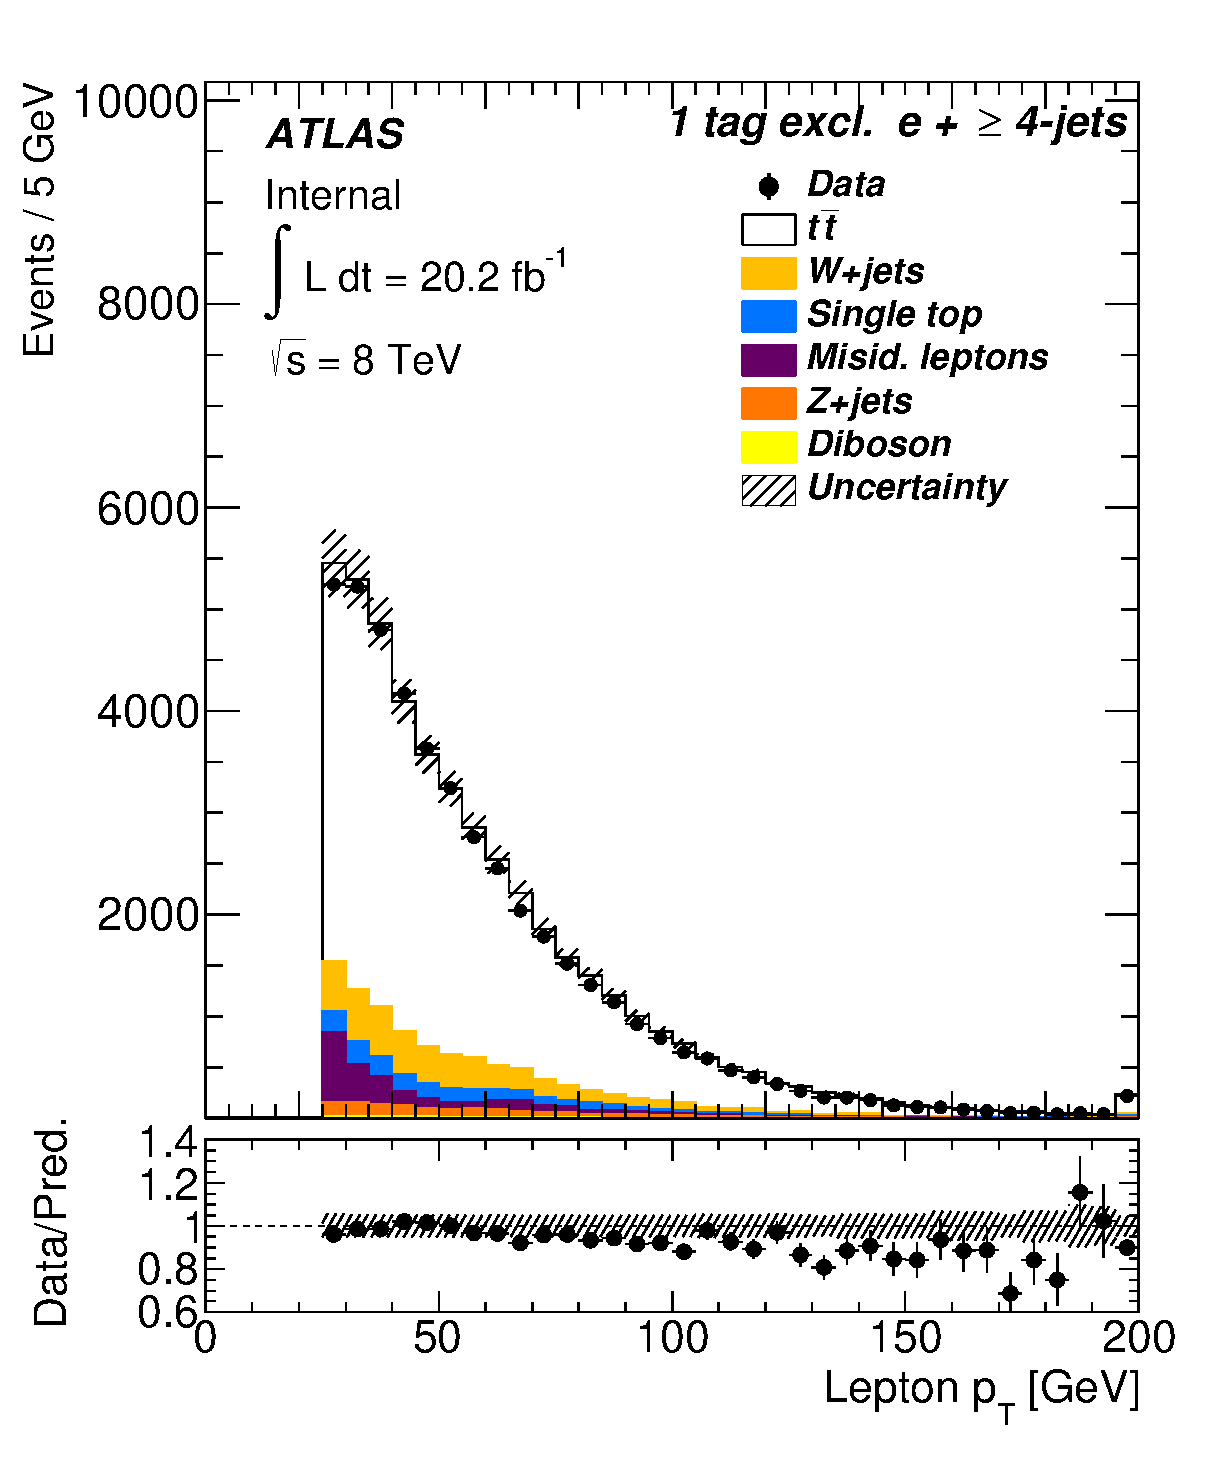
\includegraphics[height=65mm]{chapters/whel/figures/control_Plots2/bTag_1excl/LeptonPt_el}
		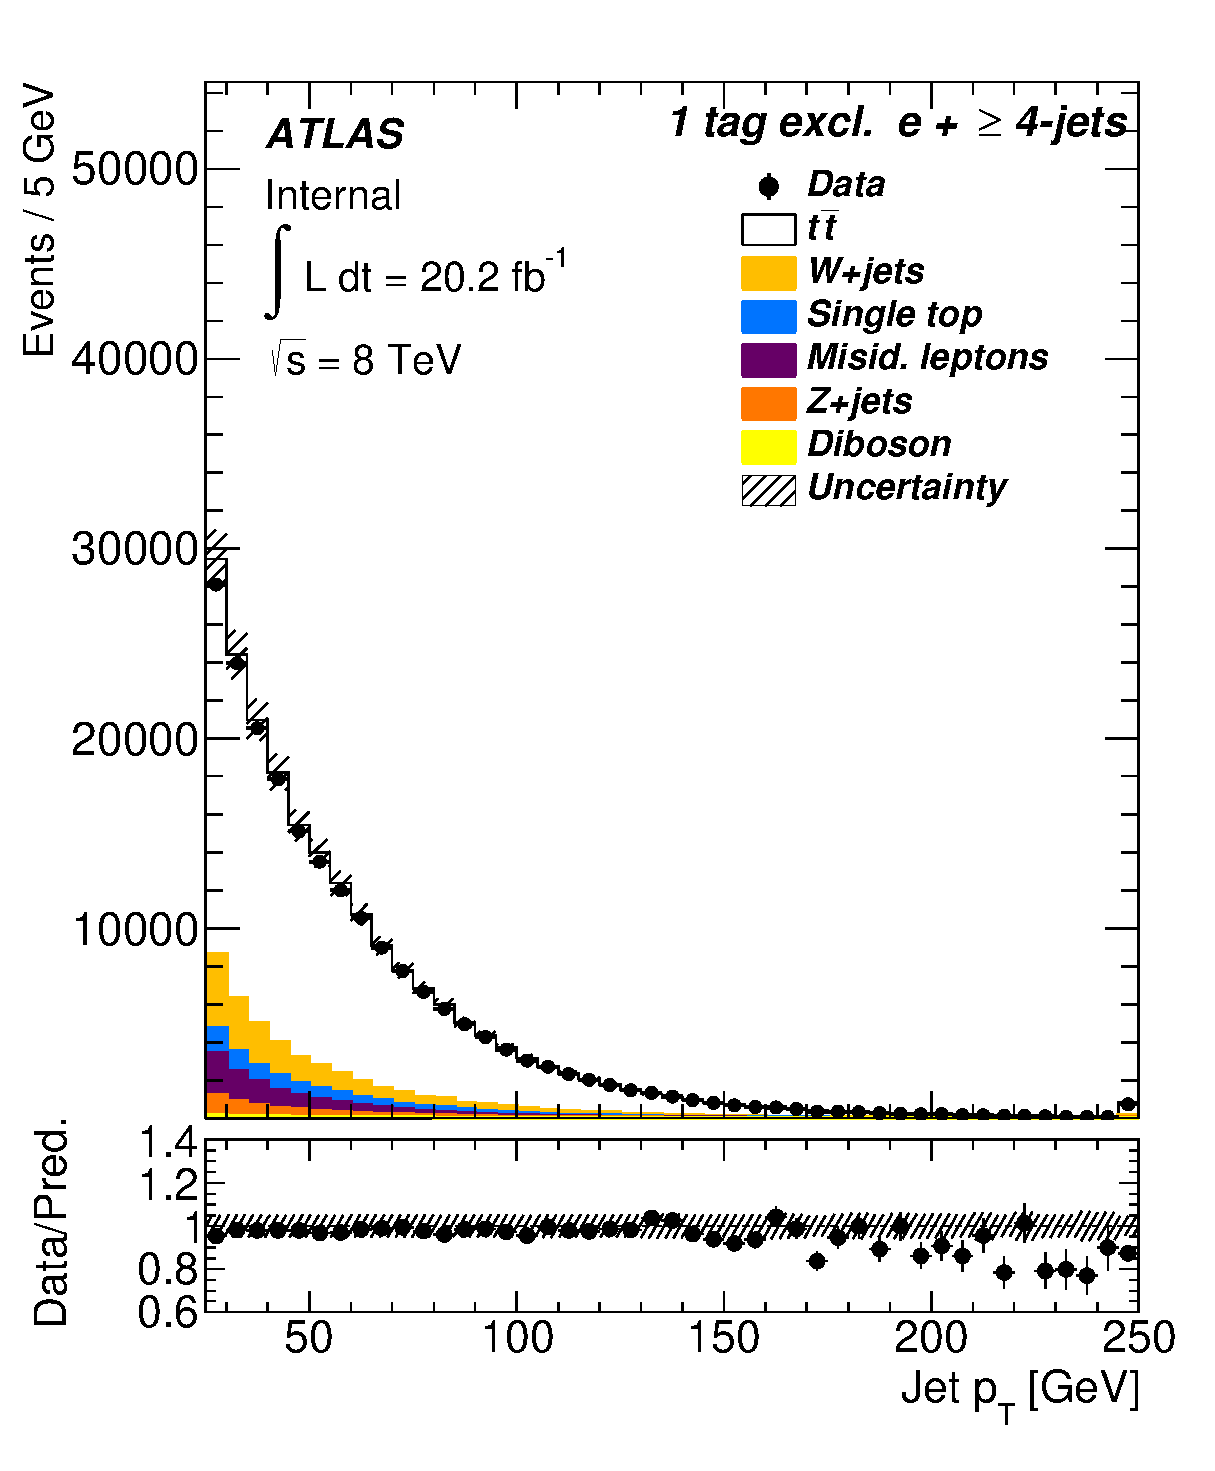
\includegraphics[height=65mm]{chapters/whel/figures/control_Plots2/bTag_1excl/JetPt_el}\\
		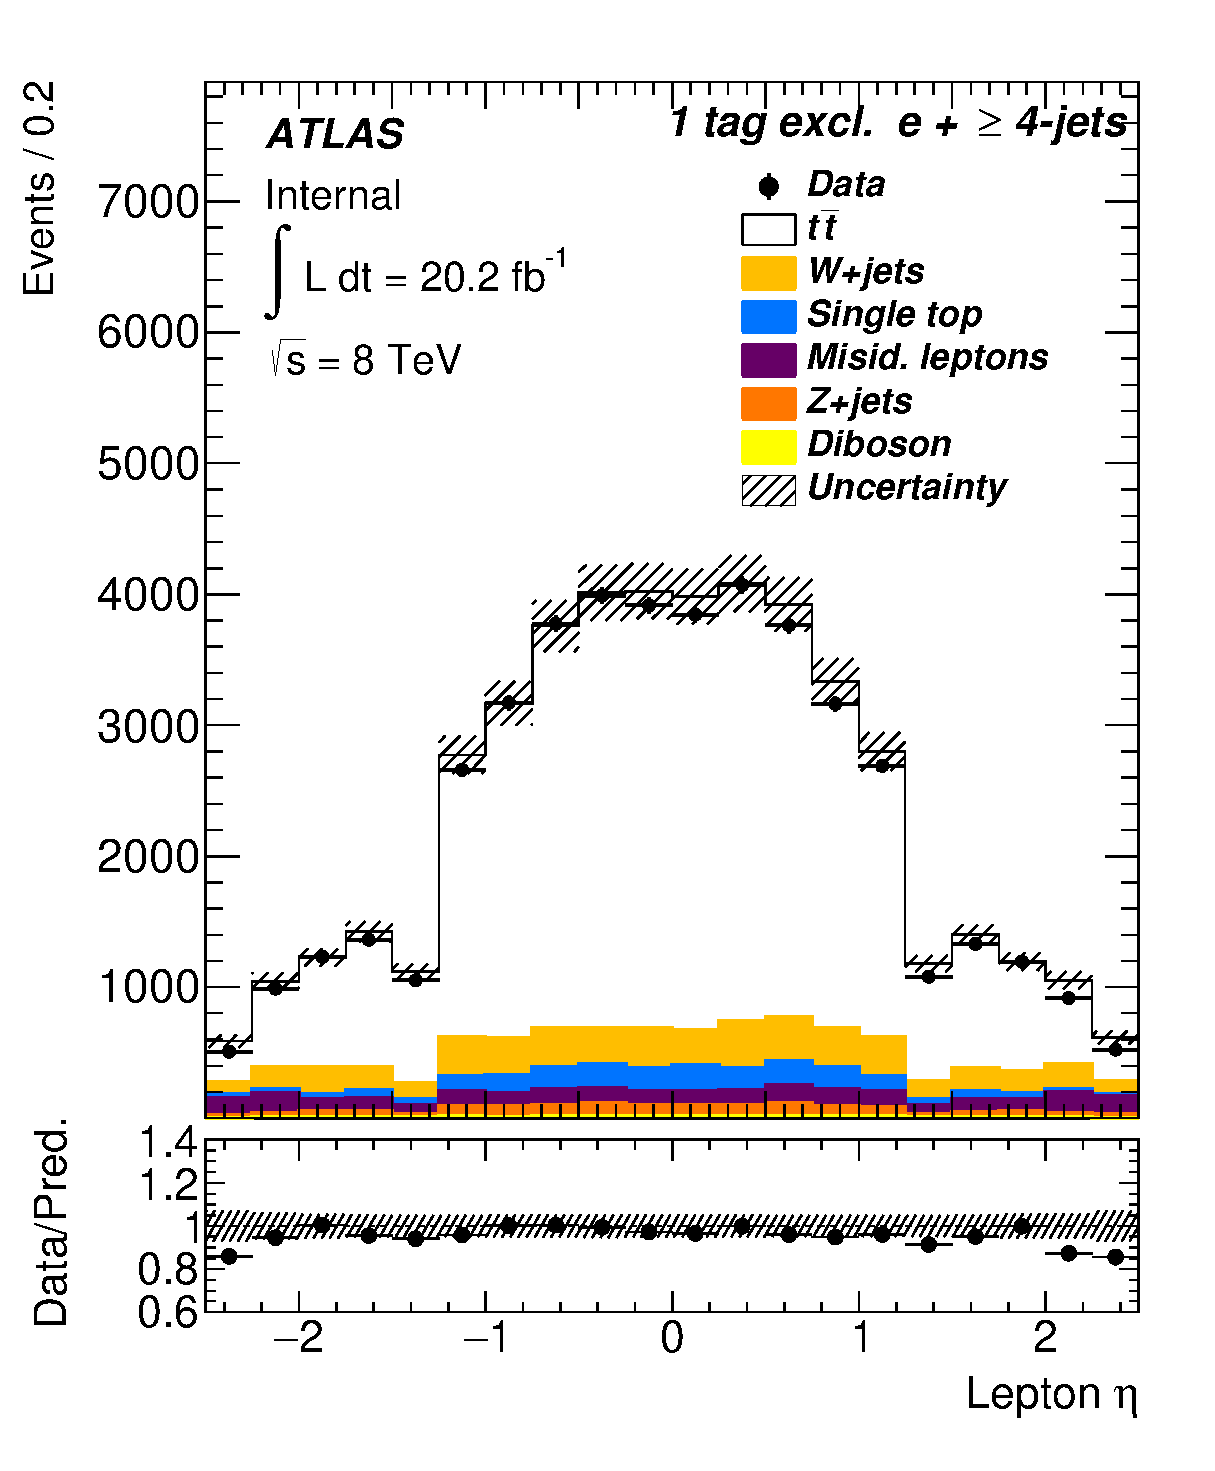
\includegraphics[height=65mm]{chapters/whel/figures/control_Plots2/bTag_1excl/LeptonEta_el}
		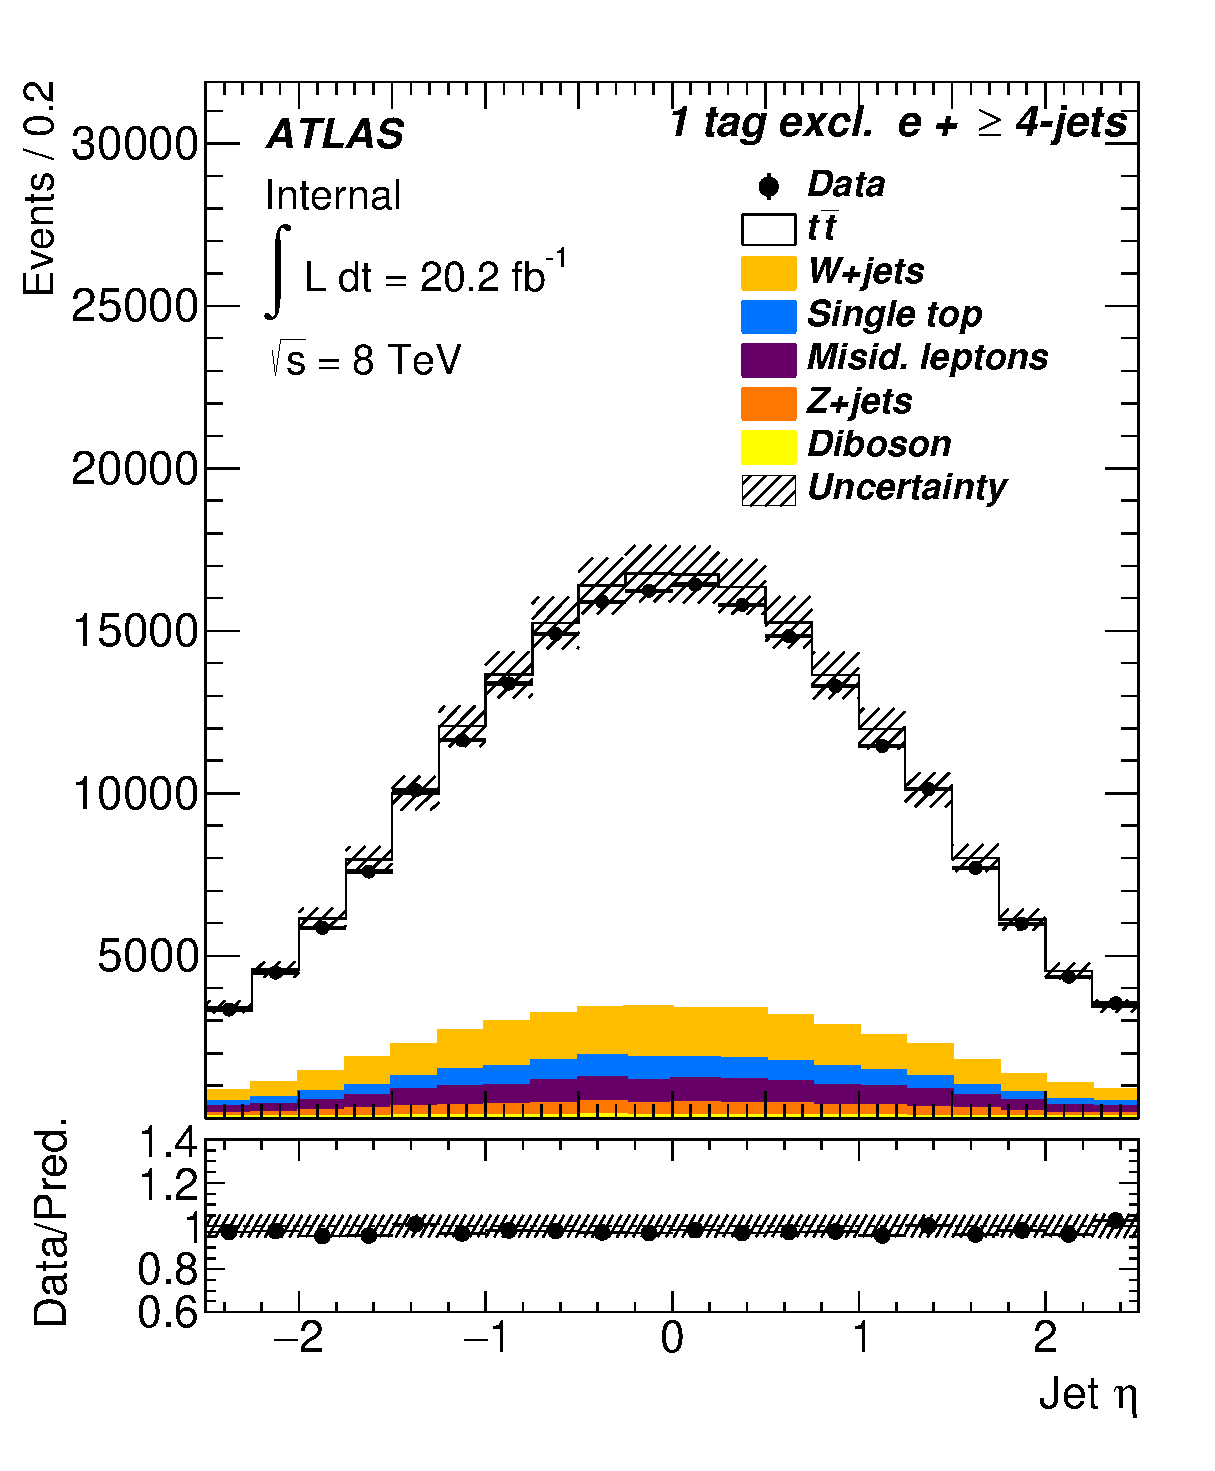
\includegraphics[height=65mm]{chapters/whel/figures/control_Plots2/bTag_1excl/JetEta_el}\\
		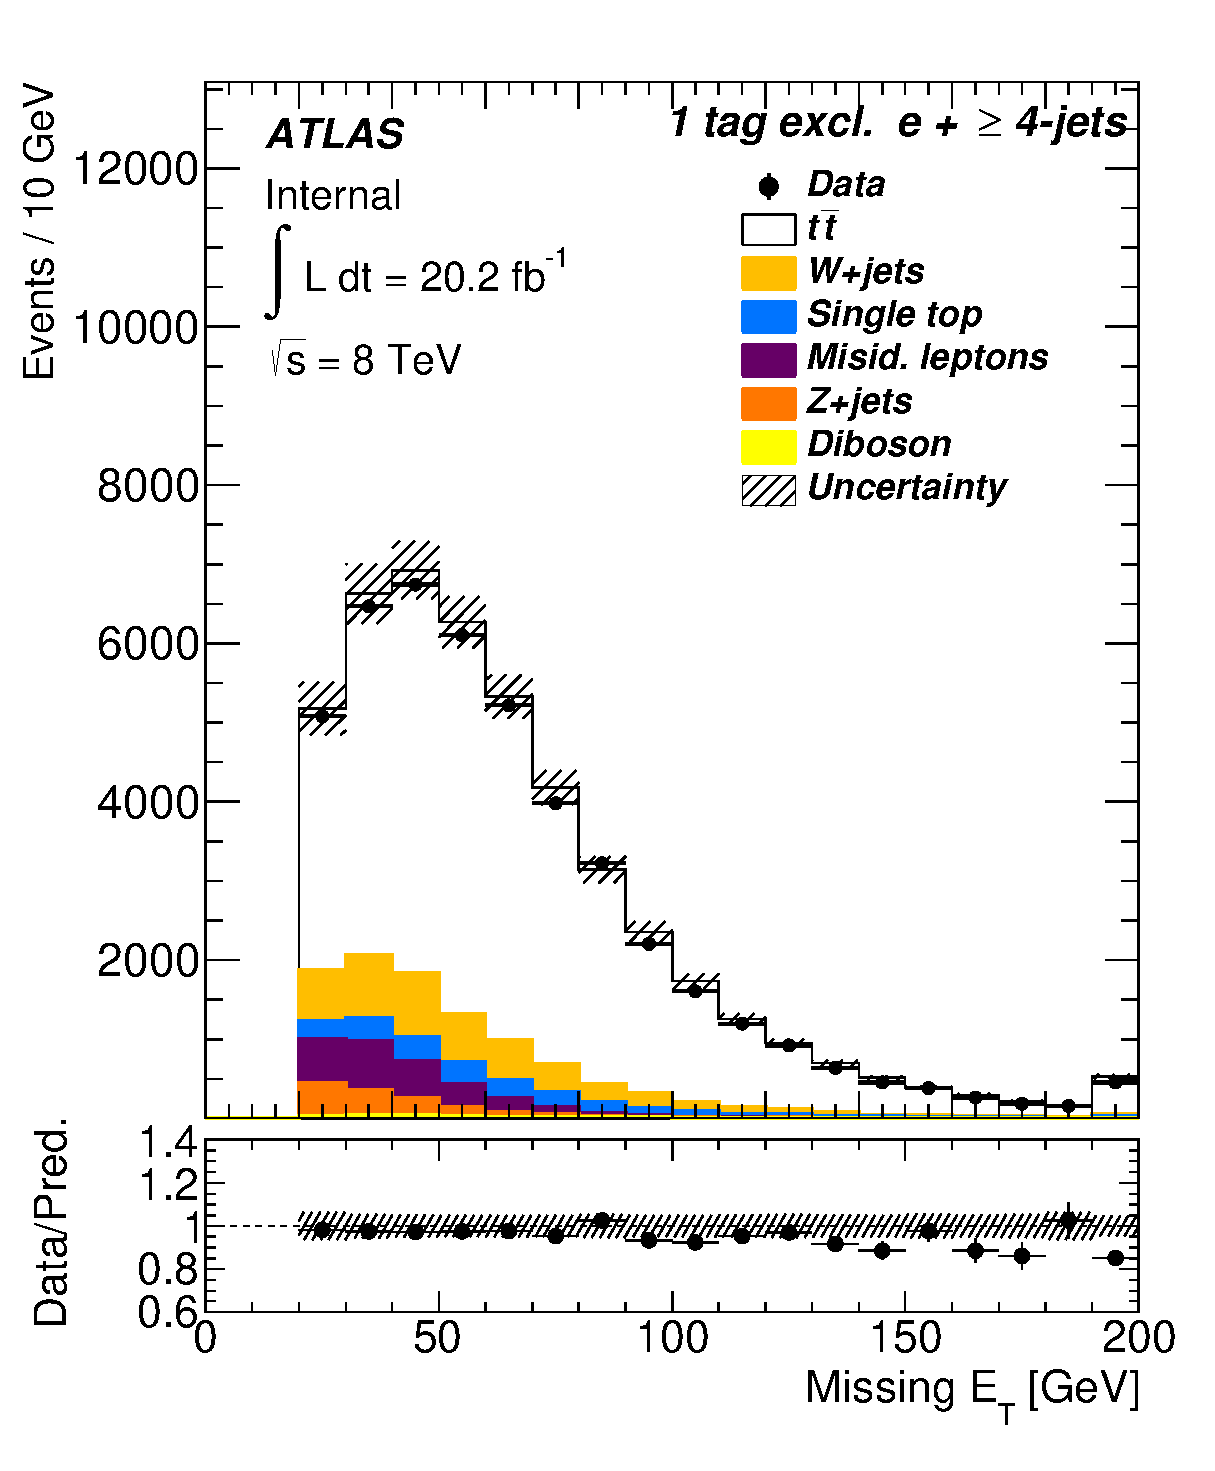
\includegraphics[height=65mm]{chapters/whel/figures/control_Plots2/bTag_1excl/MissingEt_el}
        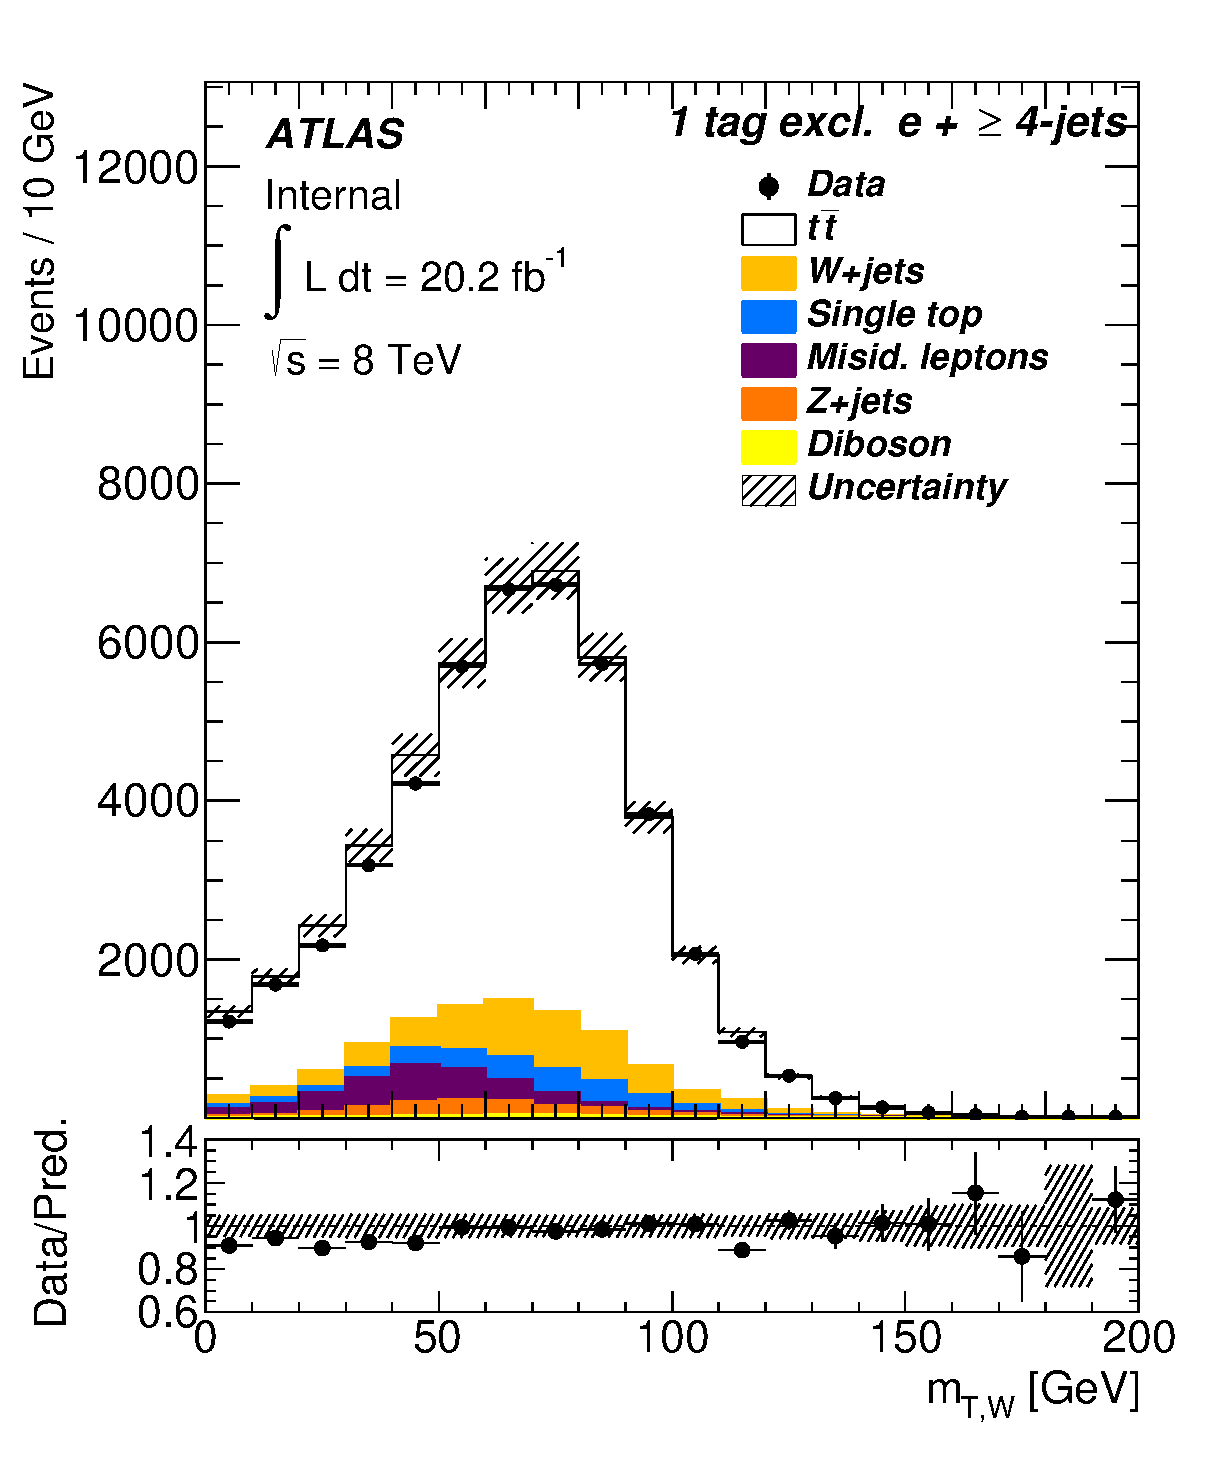
\includegraphics[height=65mm]{chapters/whel/figures/control_Plots2/bTag_1excl/TransverseMass_el}
	\caption{Plots showing data/MC agreement after event selection for reconstructed objects (lepton, jets, neutrino) in the 1 exclusive \bt tag, electron region. The shaded bands represent the Monte Carlo statistical uncertainties.}
	\label{fig:control_plots_el_1excl}
	\end{center}
	\end{figure}
	
\begin{figure}[!hb]
\begin{center}

		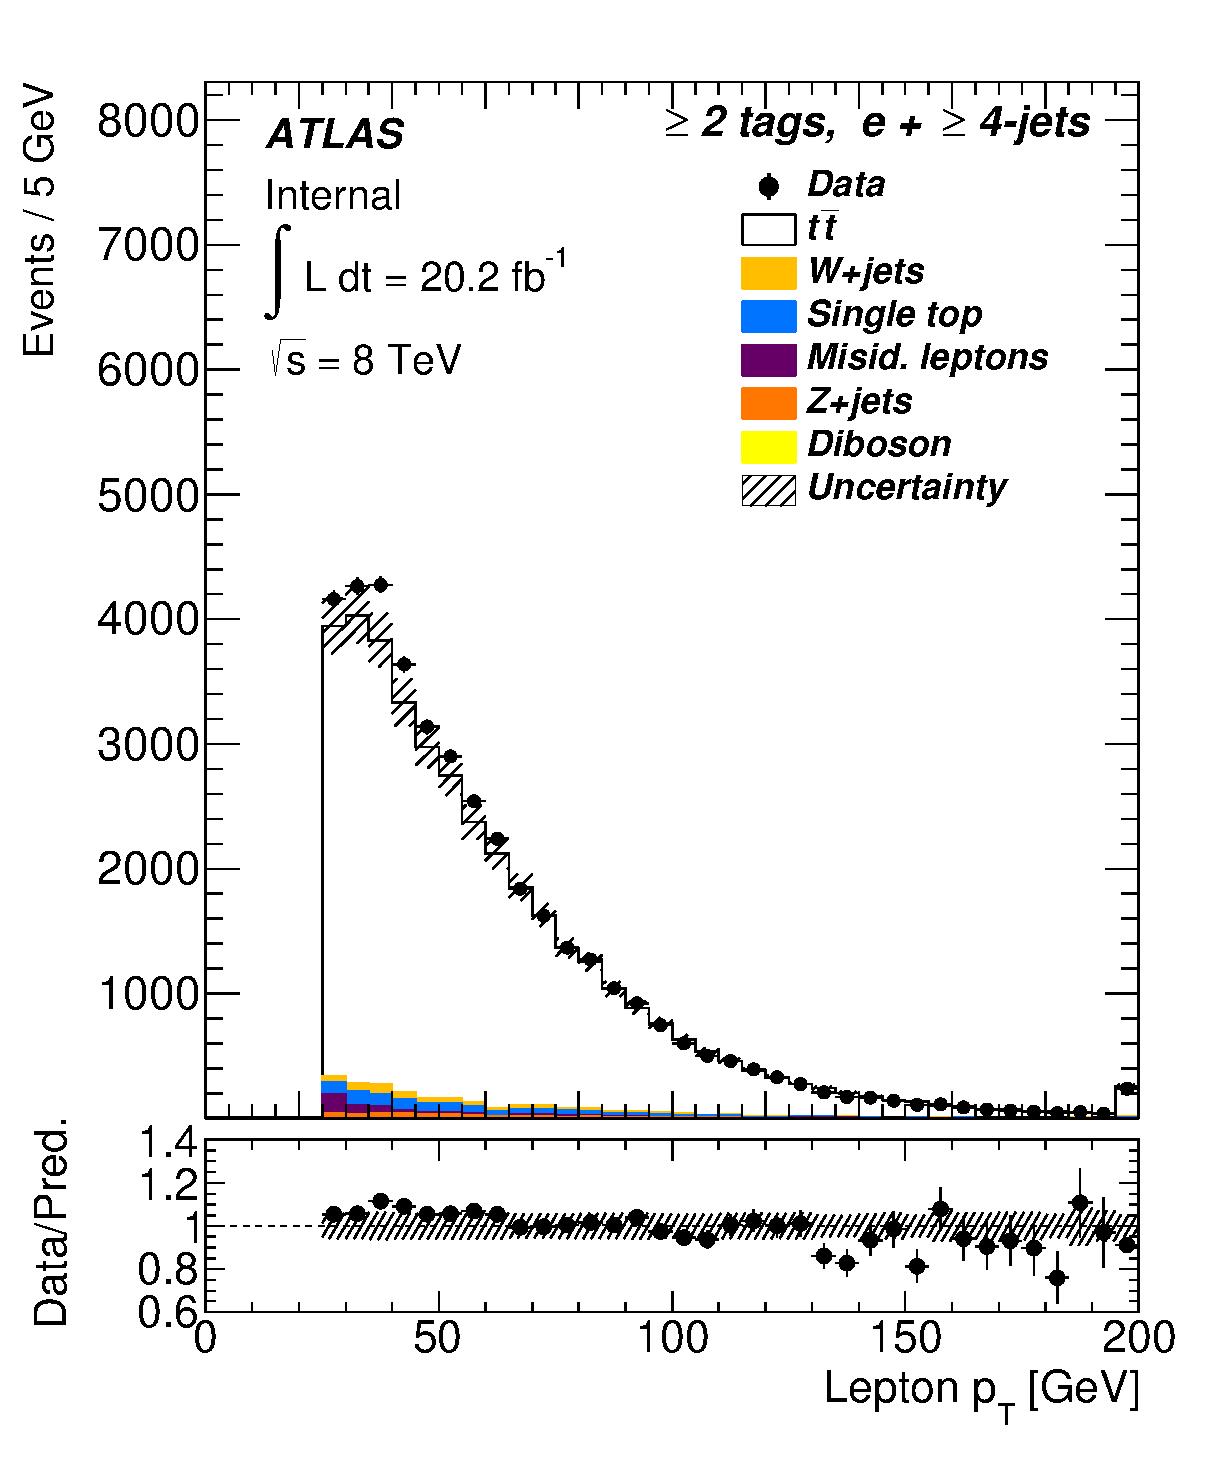
\includegraphics[height=65mm]{chapters/whel/figures/control_Plots2/bTag_2incl/LeptonPt_el}
		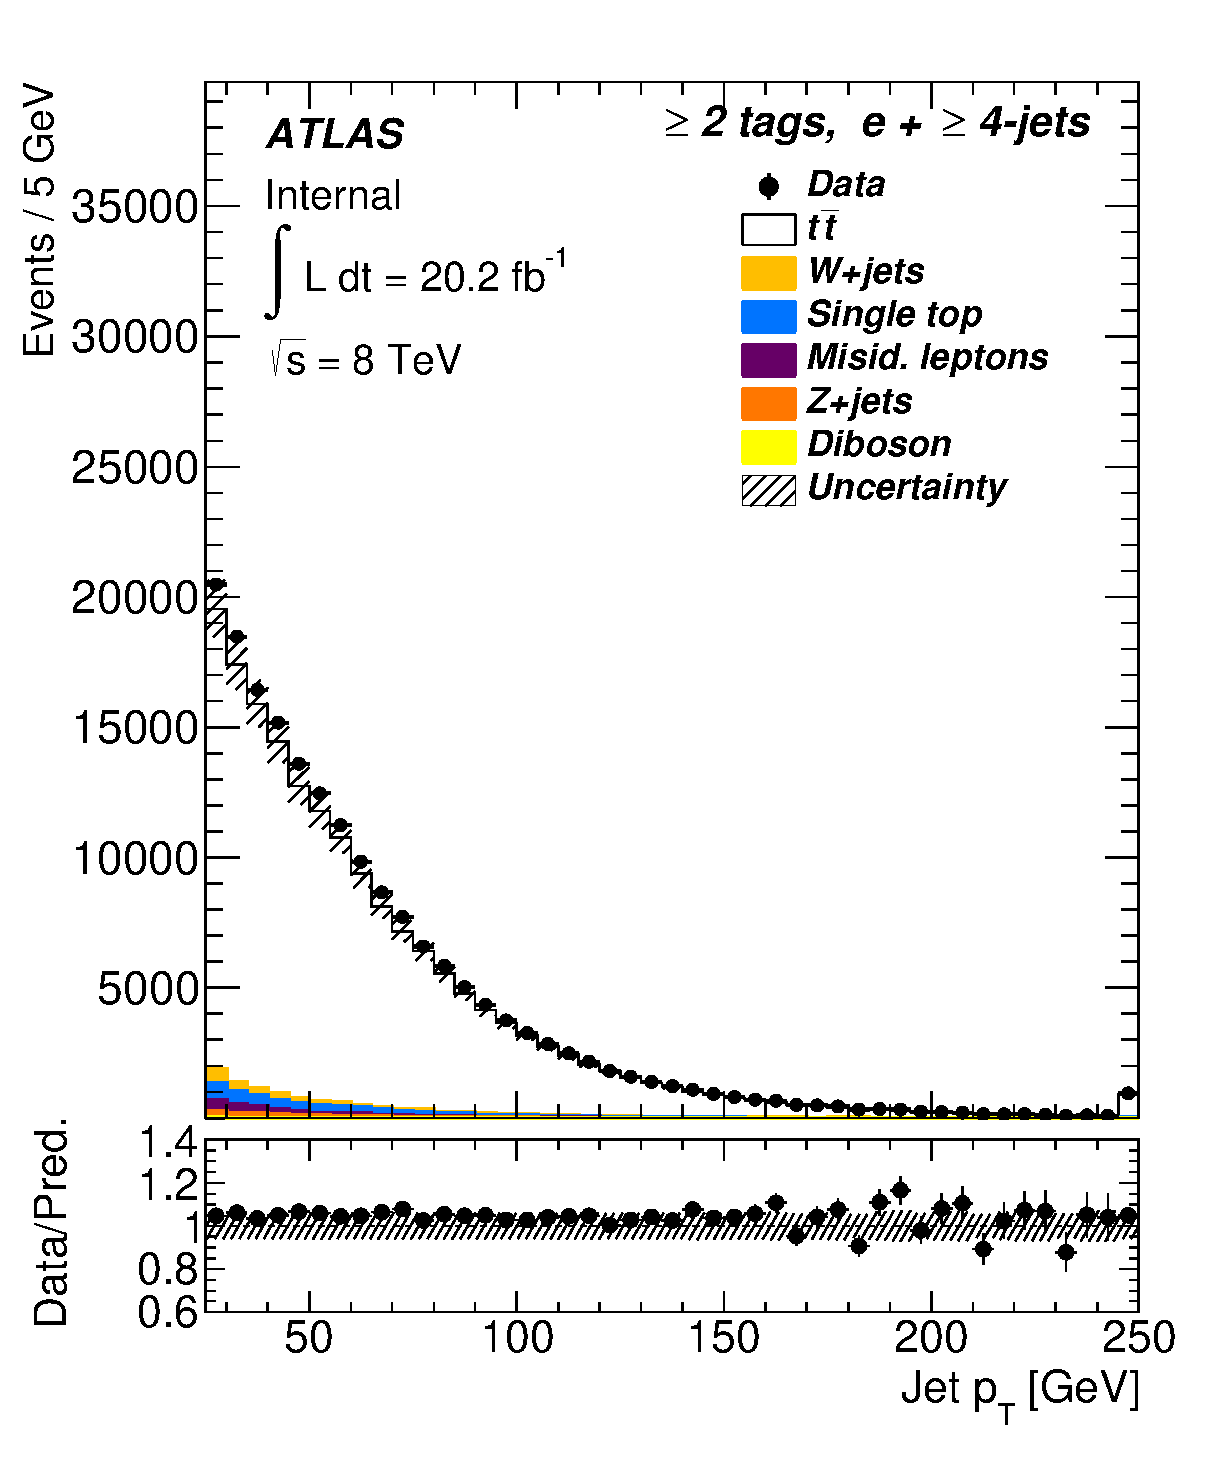
\includegraphics[height=65mm]{chapters/whel/figures/control_Plots2/bTag_2incl/JetPt_el}\\
		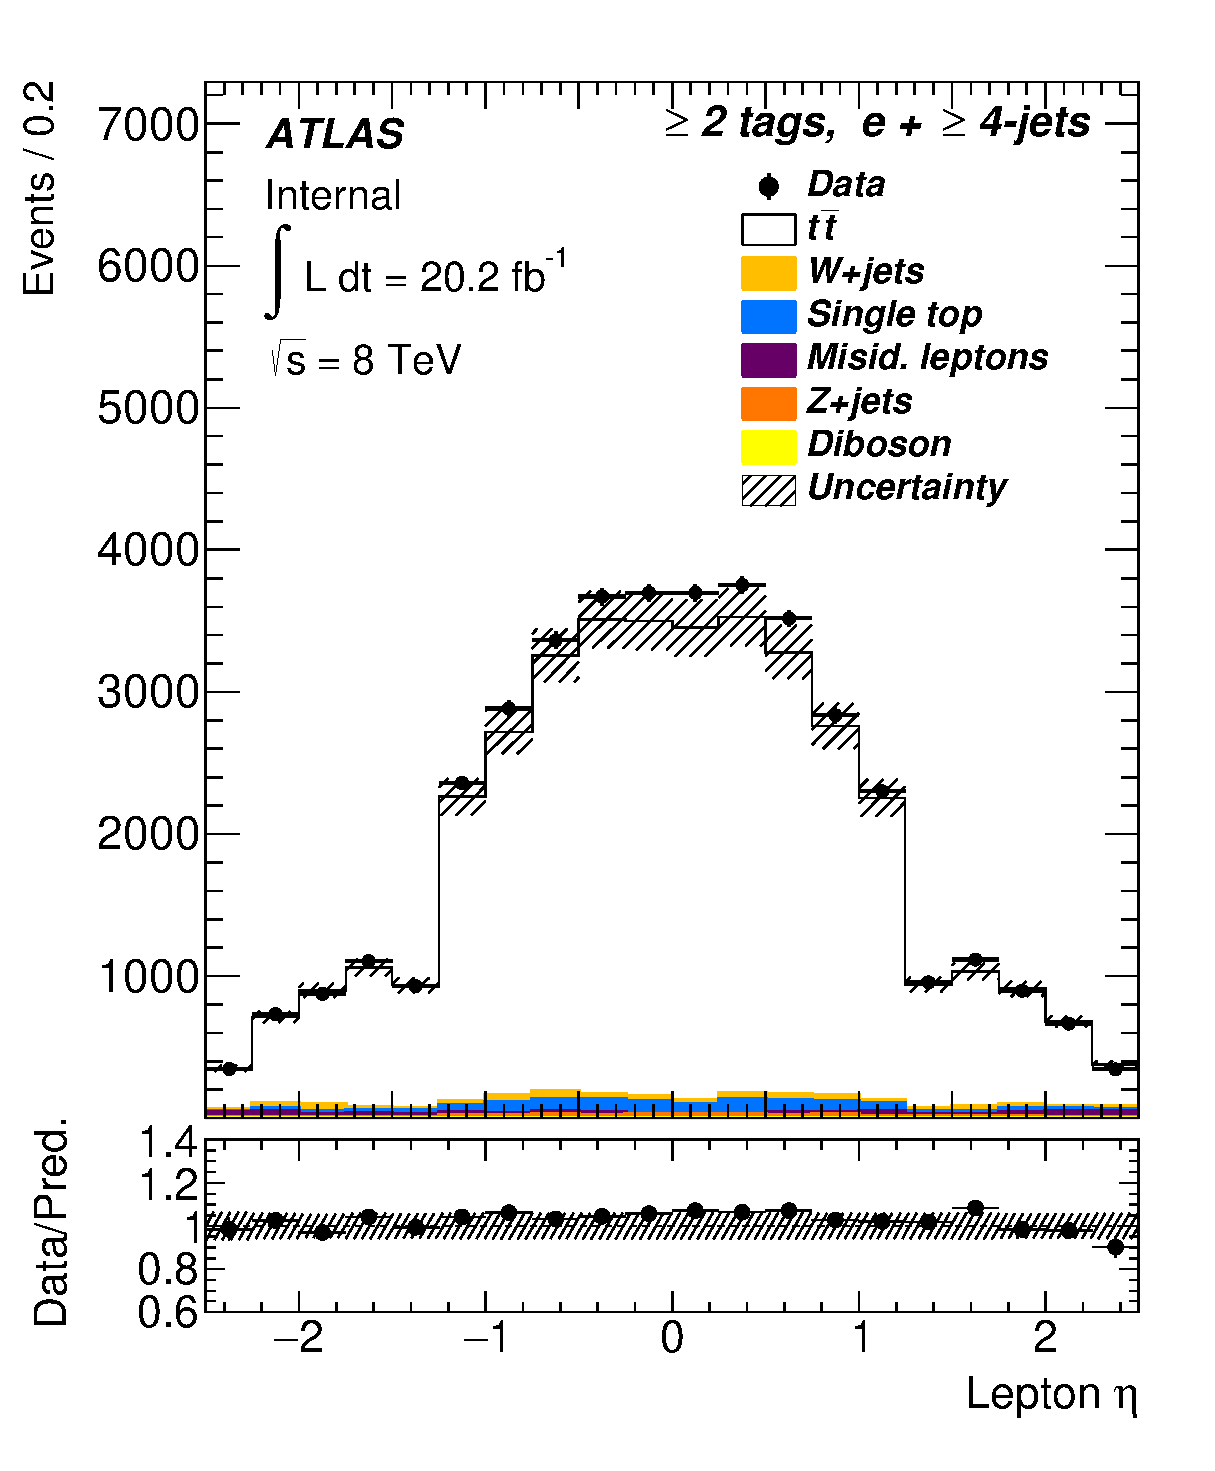
\includegraphics[height=65mm]{chapters/whel/figures/control_Plots2/bTag_2incl/LeptonEta_el}
		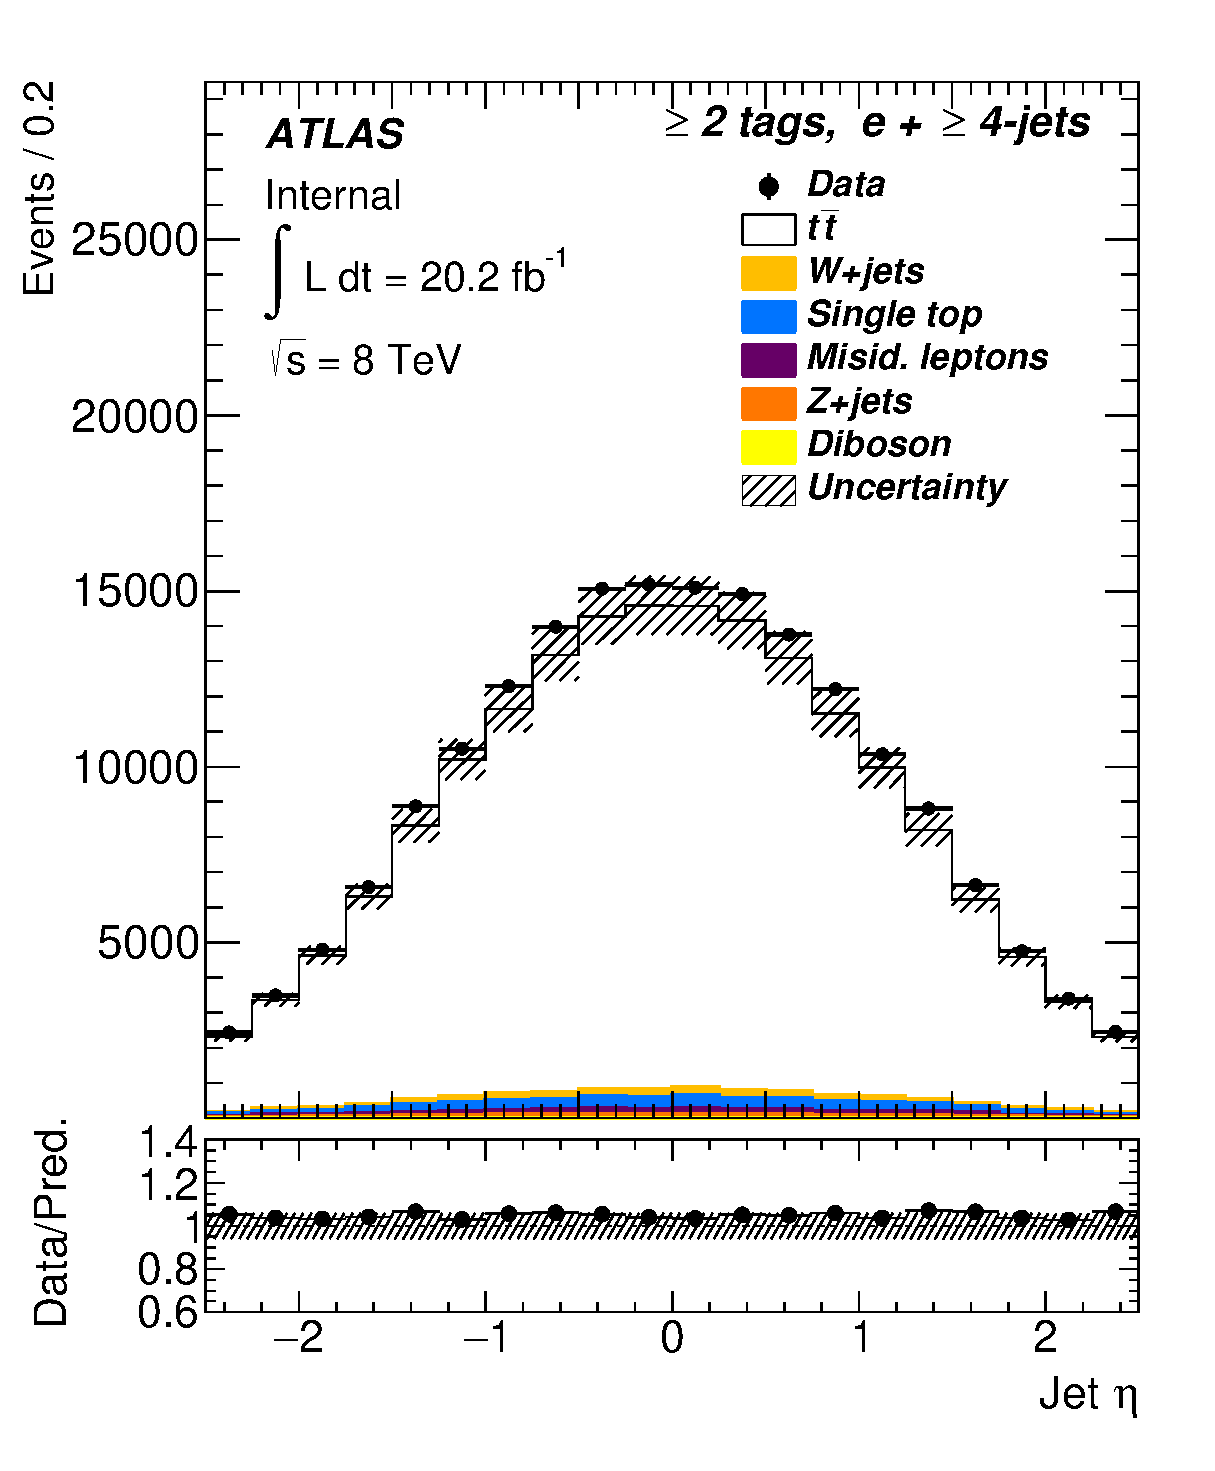
\includegraphics[height=65mm]{chapters/whel/figures/control_Plots2/bTag_2incl/JetEta_el}\\
		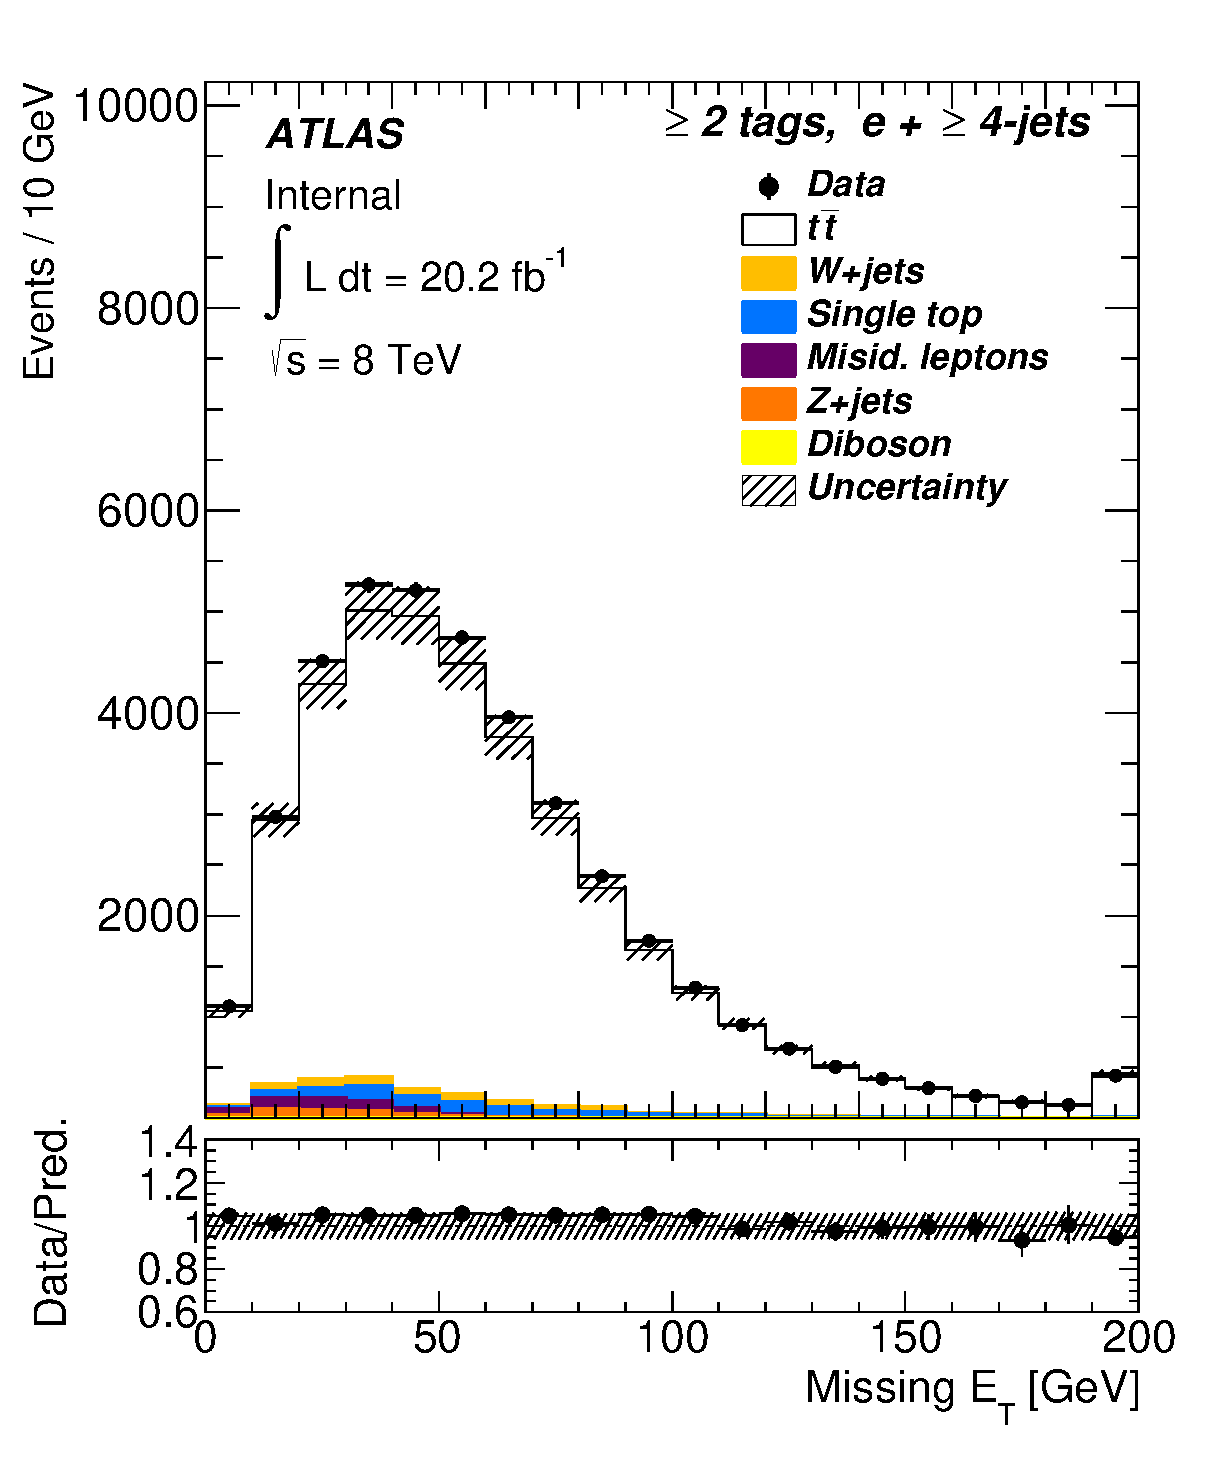
\includegraphics[height=65mm]{chapters/whel/figures/control_Plots2/bTag_2incl/MissingEt_el}
        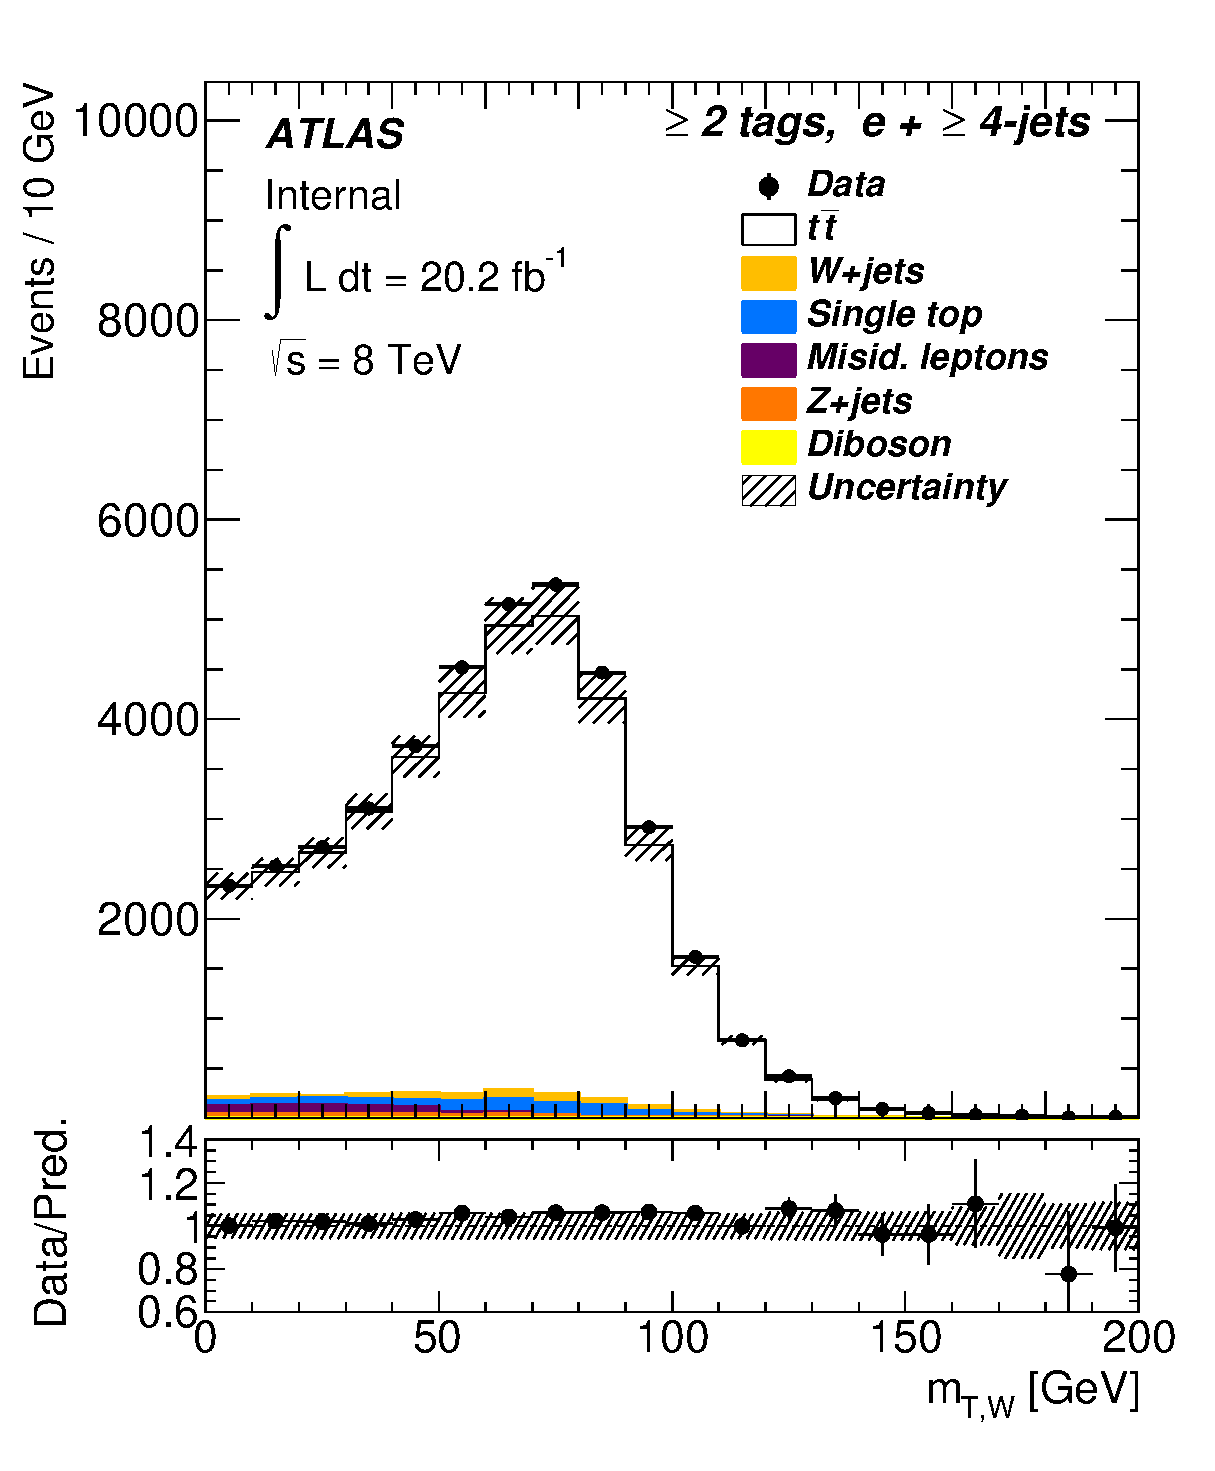
\includegraphics[height=65mm]{chapters/whel/figures/control_Plots2/bTag_2incl/TransverseMass_el}
	\caption{Plots showing data/MC agreement after event selection for reconstructed objects (lepton, jets, neutrino) in the 2 inclusive \bt tag, electron region. The shaded bands represent the Monte Carlo statistical uncertainties.}
	\label{fig:control_plots_el_2incl}
	\end{center}
	\end{figure}
	

\begin{figure}[!hb]
\begin{center}

		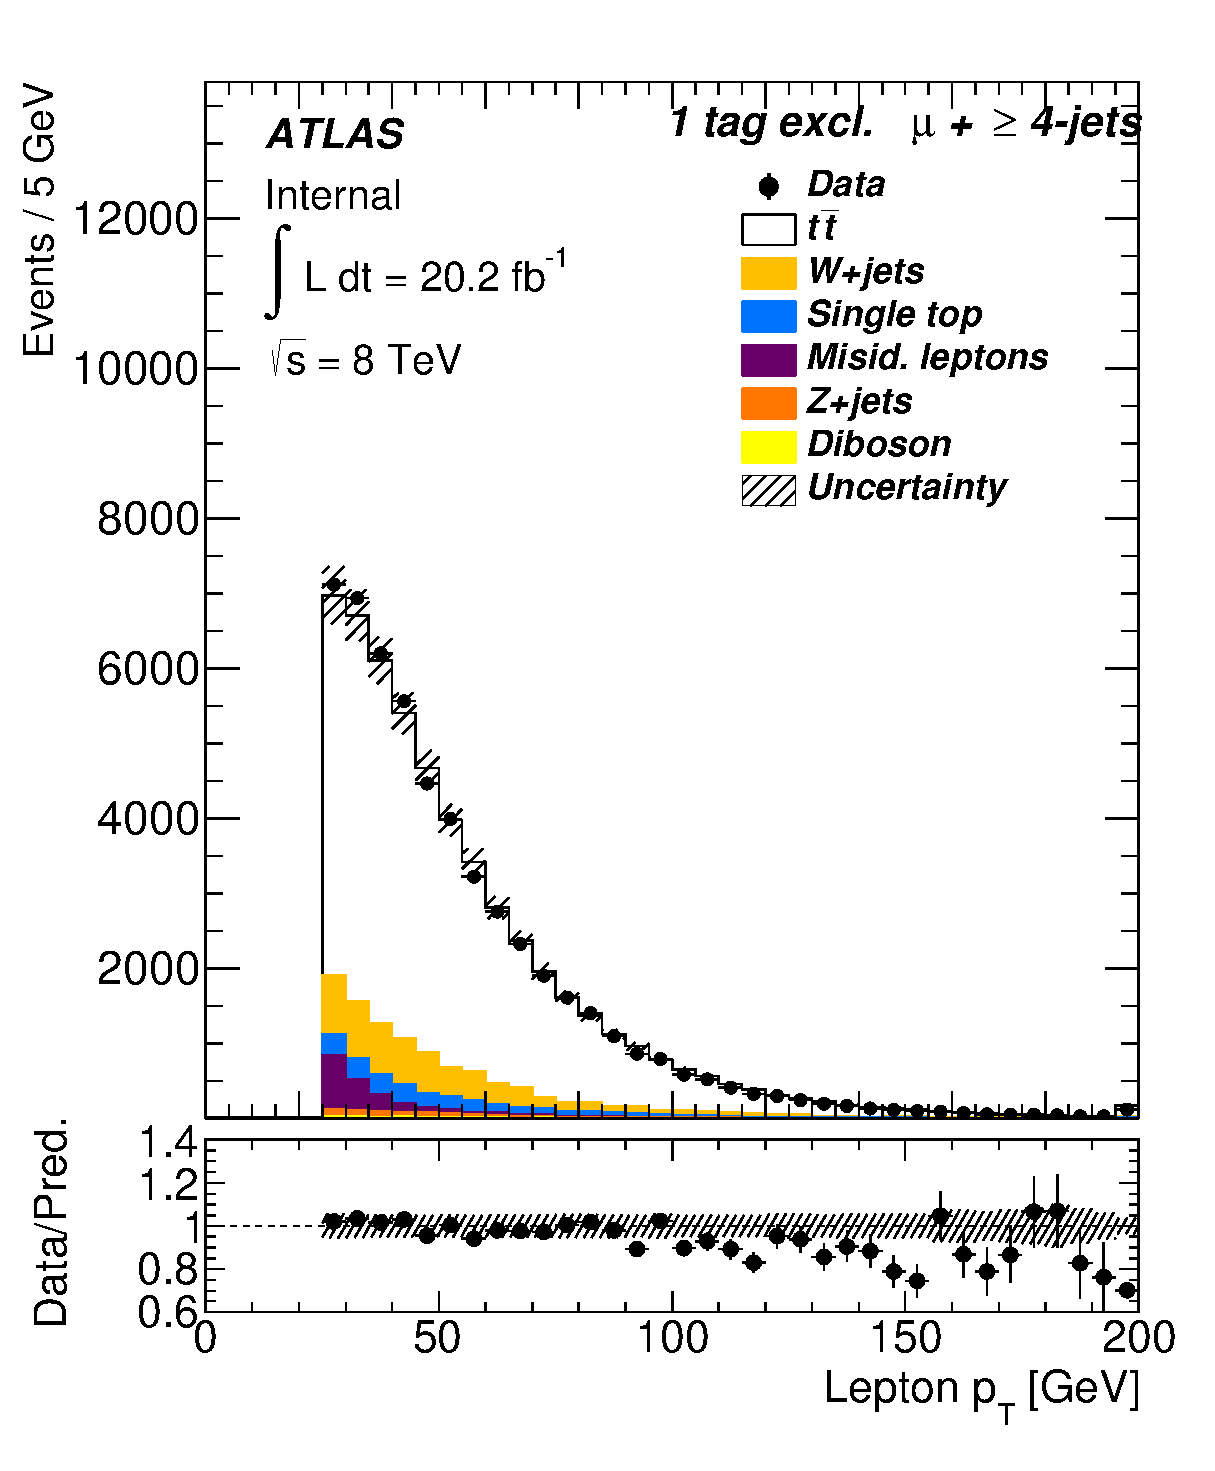
\includegraphics[height=65mm]{chapters/whel/figures/control_Plots2/bTag_1excl/LeptonPt_mu}
		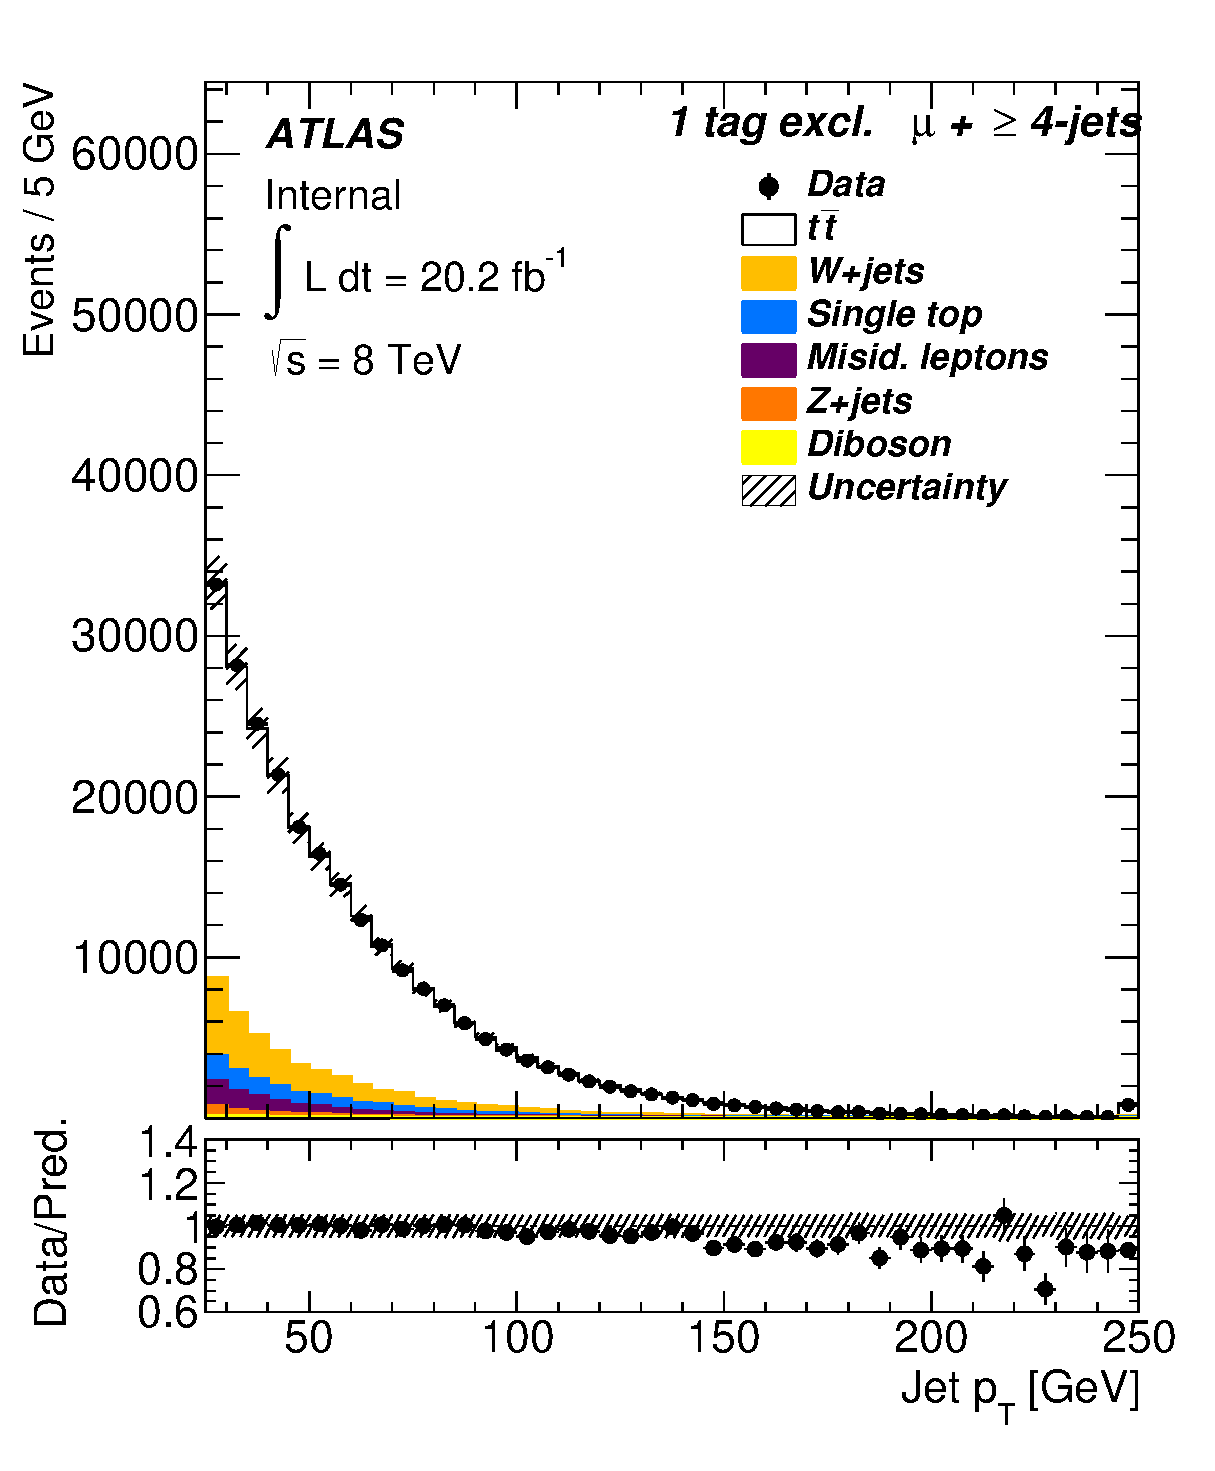
\includegraphics[height=65mm]{chapters/whel/figures/control_Plots2/bTag_1excl/JetPt_mu}\\
		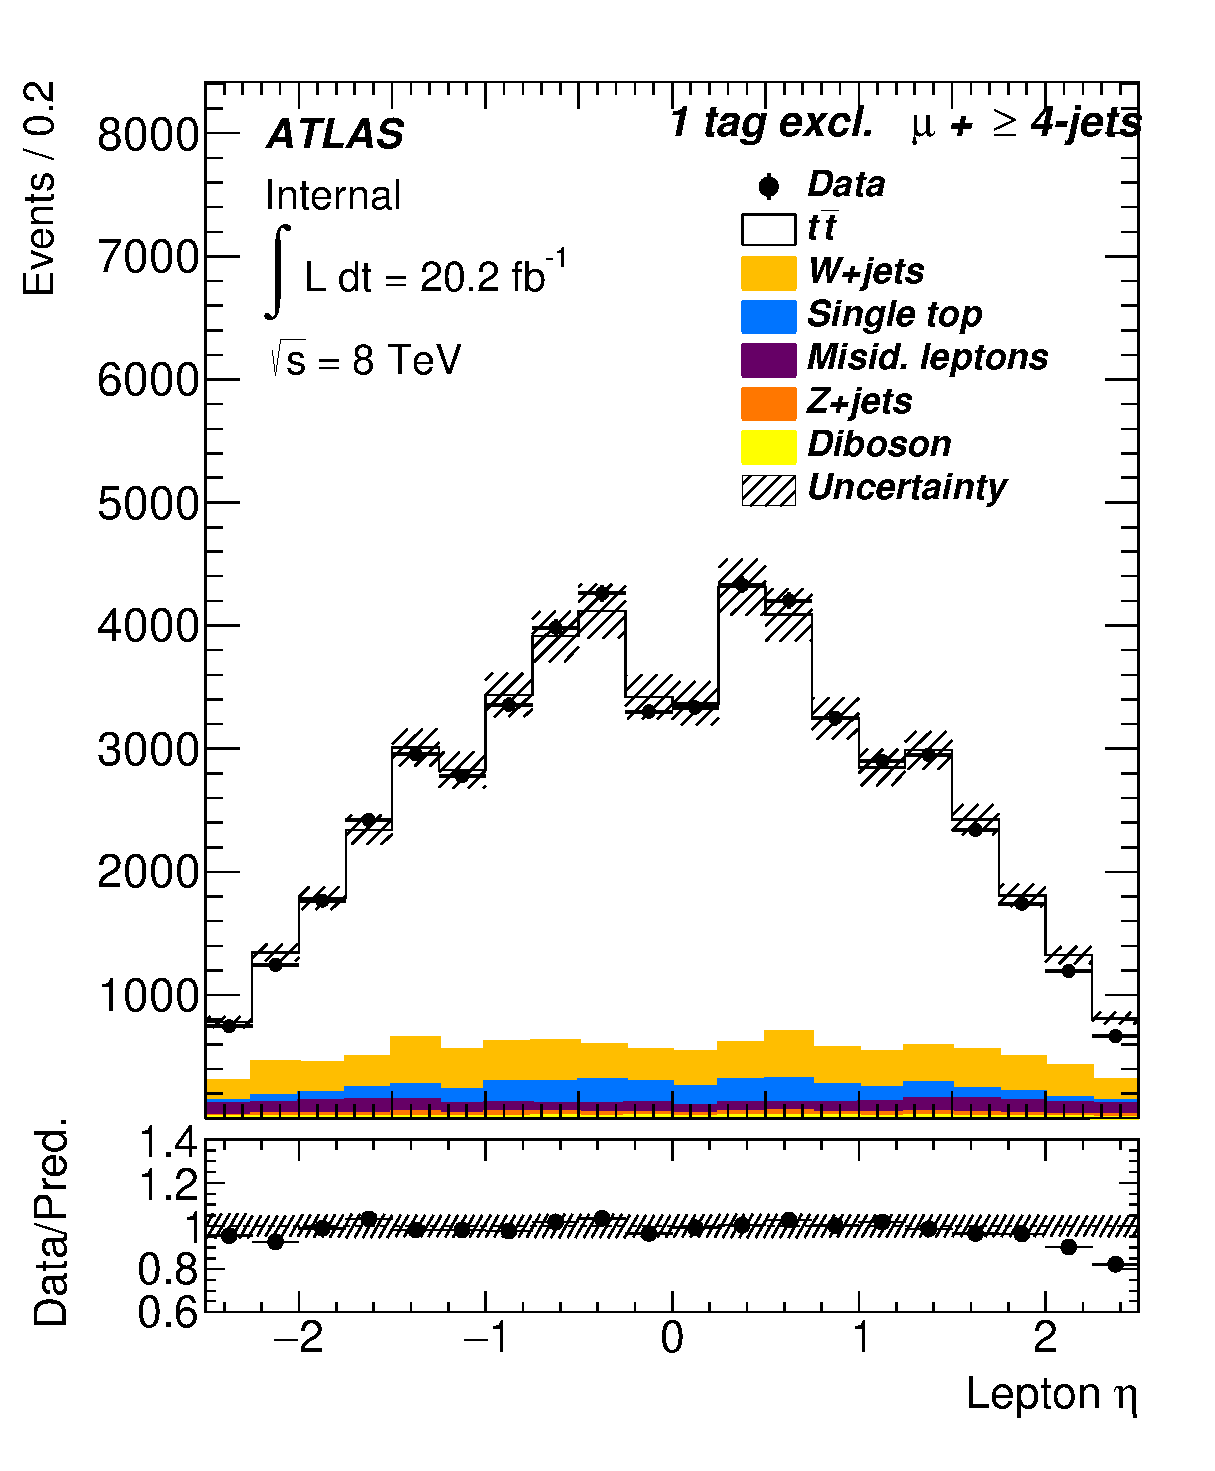
\includegraphics[height=65mm]{chapters/whel/figures/control_Plots2/bTag_1excl/LeptonEta_mu}
		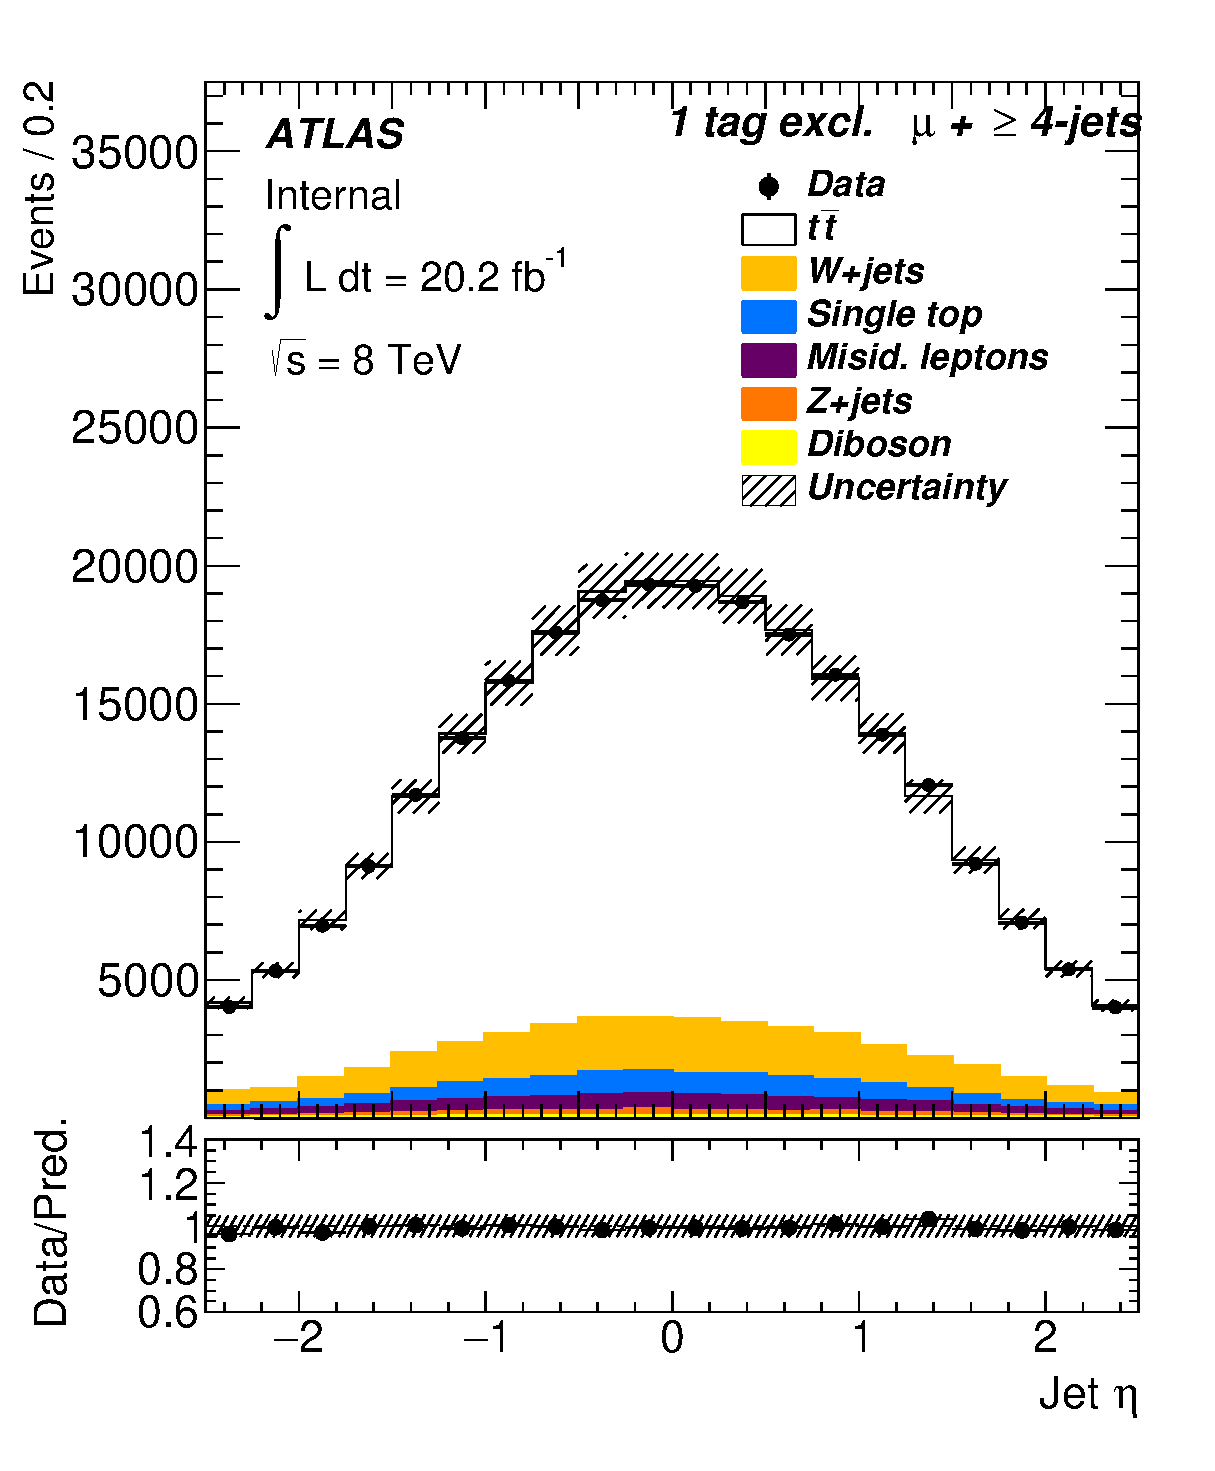
\includegraphics[height=65mm]{chapters/whel/figures/control_Plots2/bTag_1excl/JetEta_mu}\\
		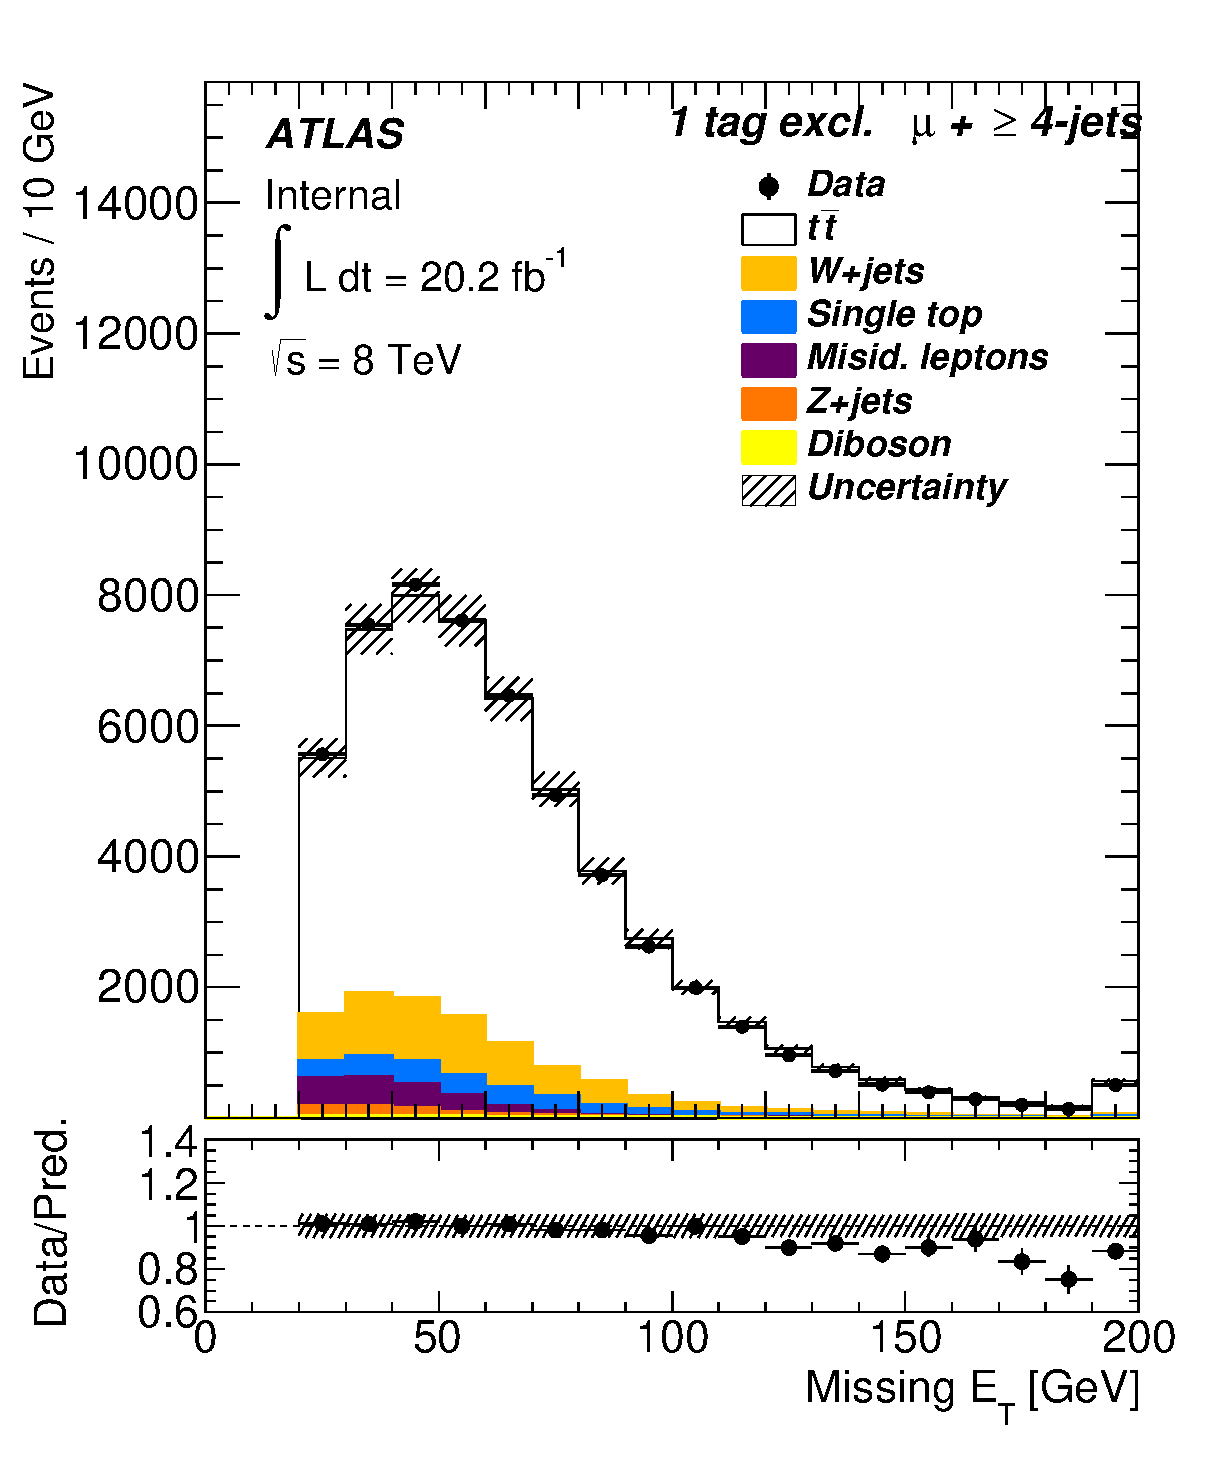
\includegraphics[height=65mm]{chapters/whel/figures/control_Plots2/bTag_1excl/MissingEt_mu}
        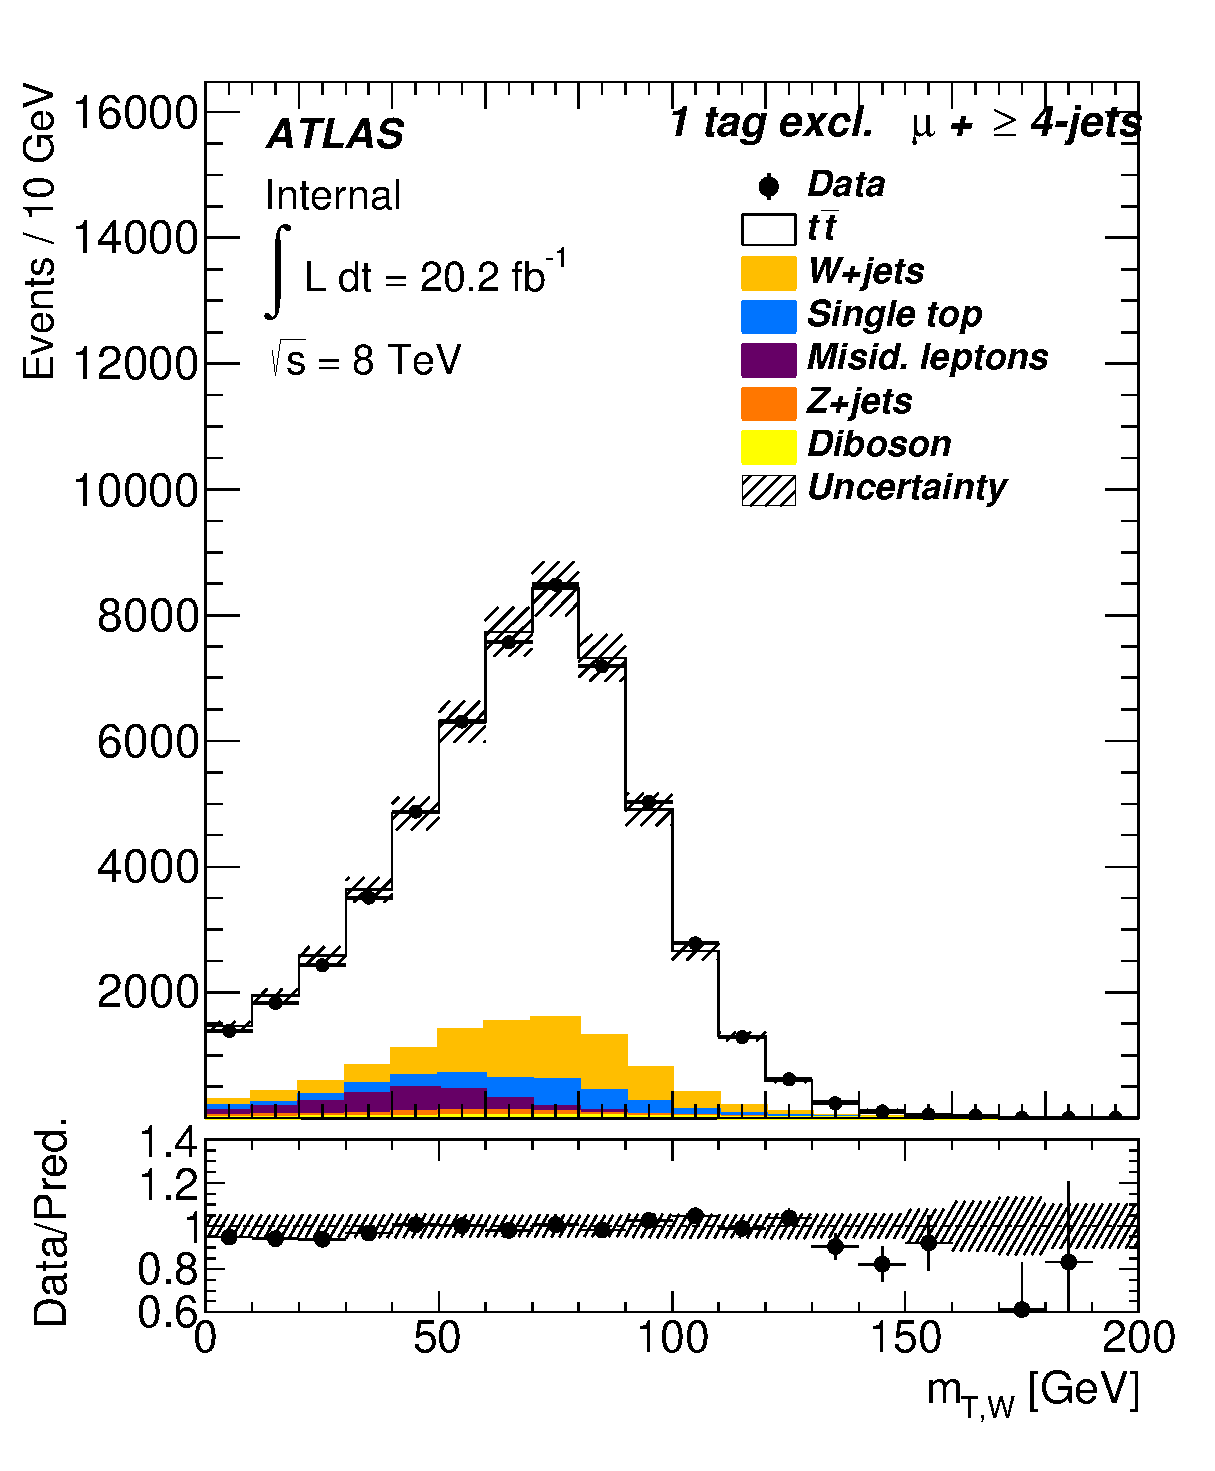
\includegraphics[height=65mm]{chapters/whel/figures/control_Plots2/bTag_1excl/TransverseMass_mu}
	\caption{Plots showing data/MC agreement after event selection for reconstructed objects (lepton, jets, neutrino) in the 1 exclusive \bt tag, muon region. The shaded bands represent the Monte Carlo statistical uncertainties.}
	\label{fig:control_plots_mu_1excl}
	\end{center}
	\end{figure}
	
\begin{figure}[!hb]
\begin{center}

		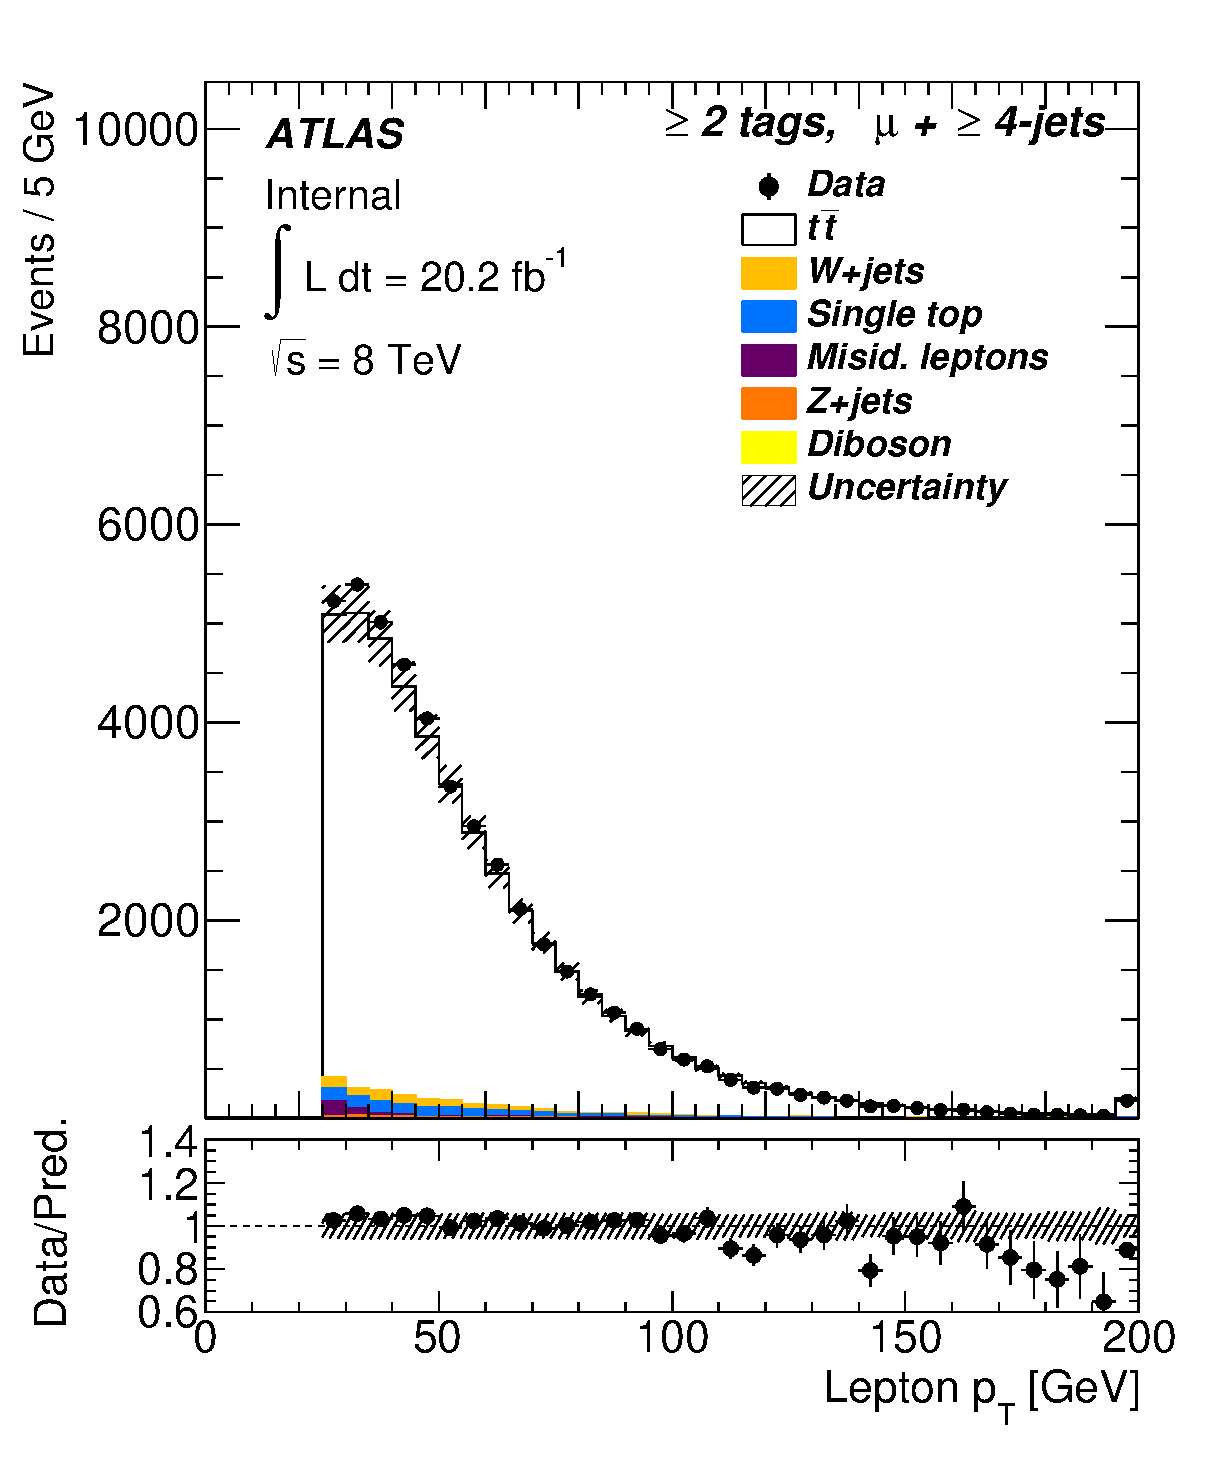
\includegraphics[height=65mm]{chapters/whel/figures/control_Plots2/bTag_2incl/LeptonPt_mu}
		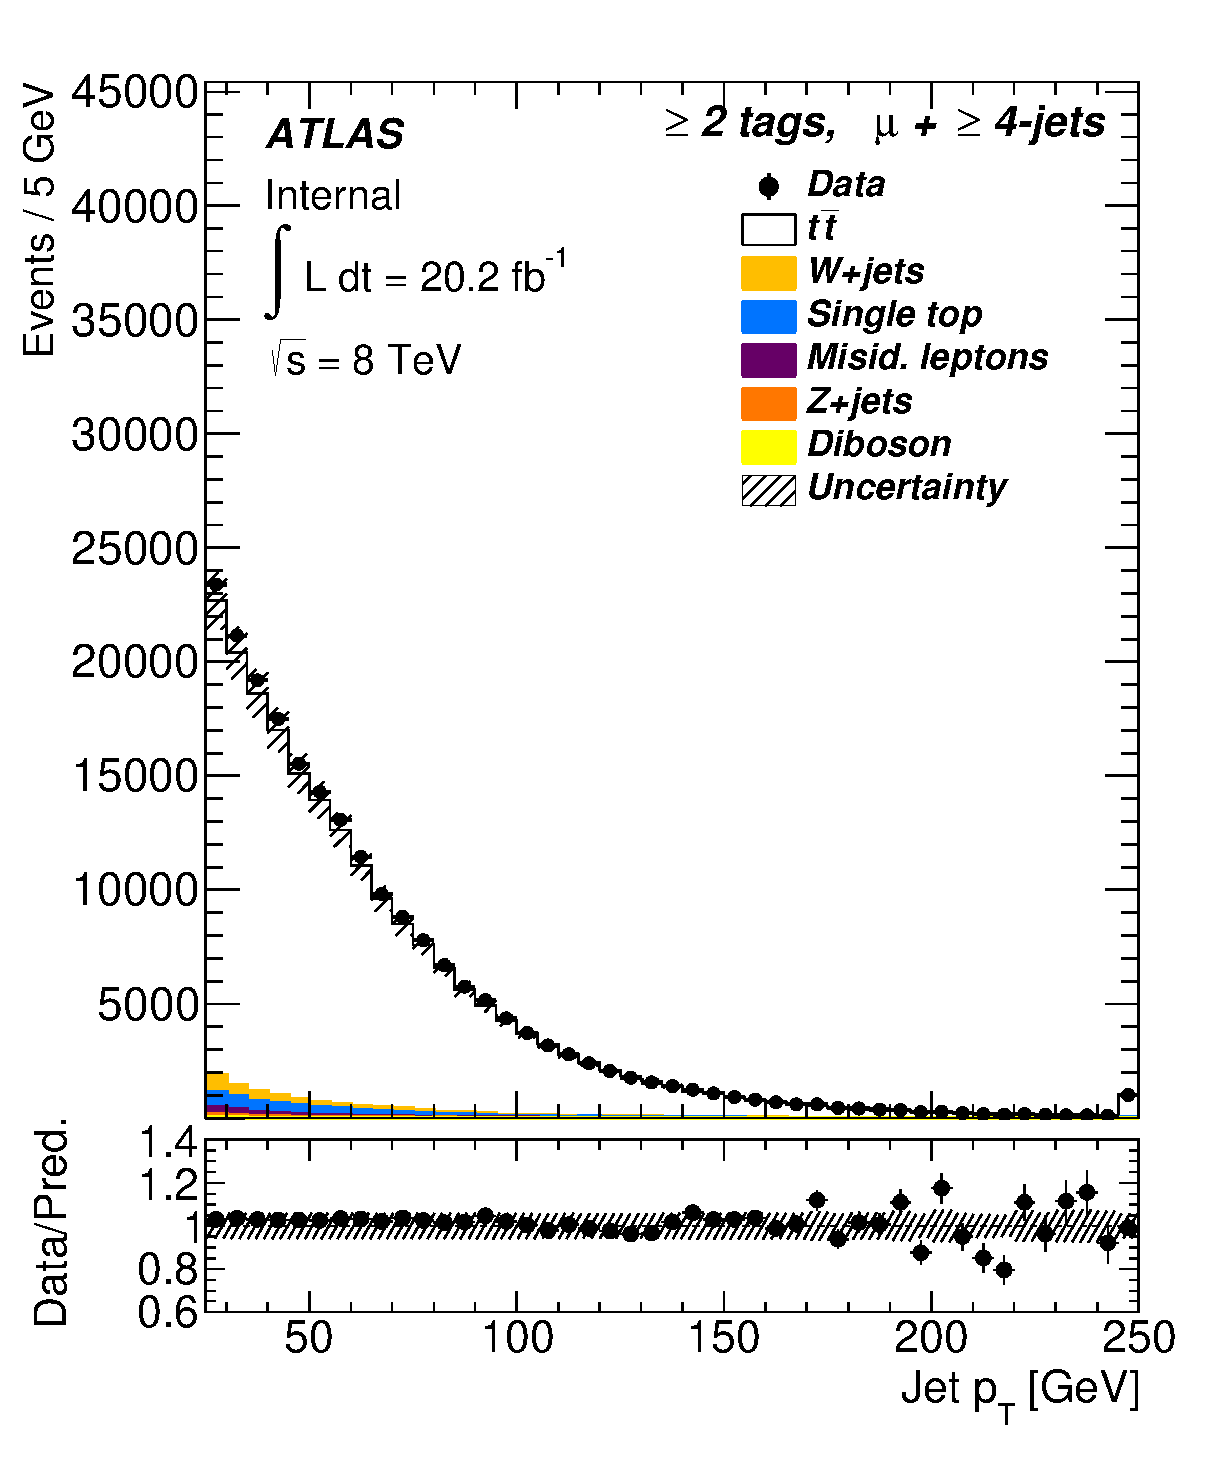
\includegraphics[height=65mm]{chapters/whel/figures/control_Plots2/bTag_2incl/JetPt_mu}\\
		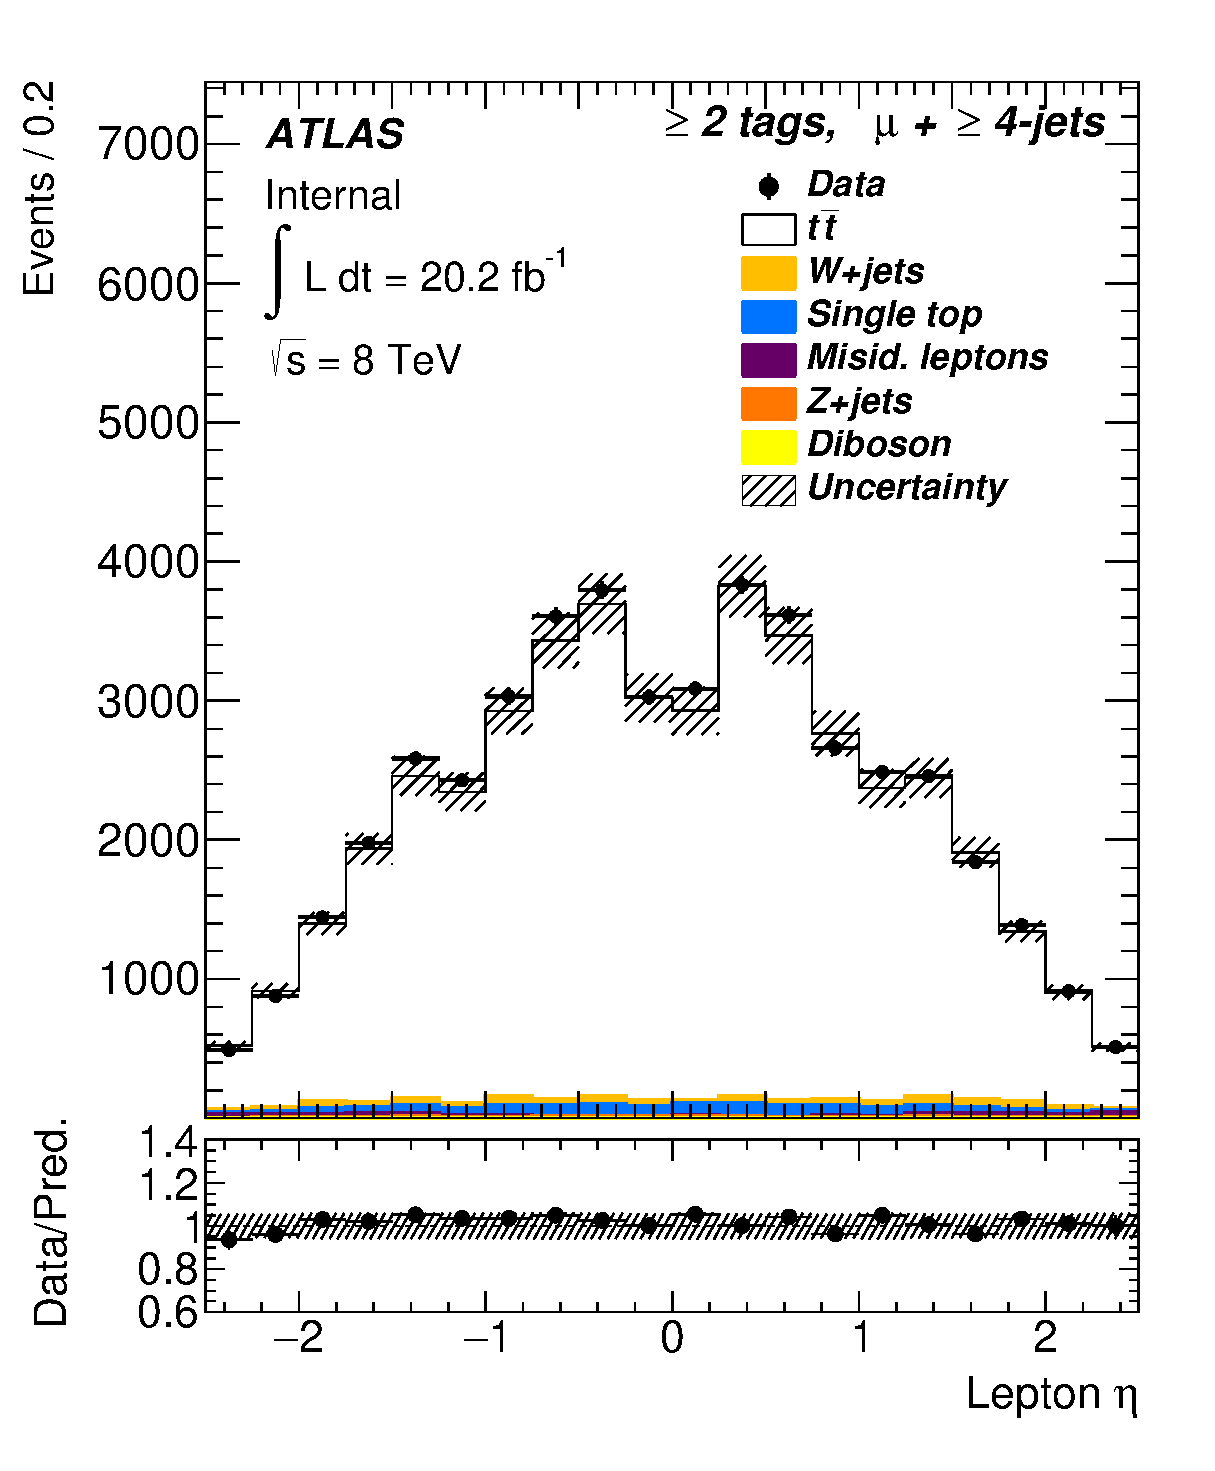
\includegraphics[height=65mm]{chapters/whel/figures/control_Plots2/bTag_2incl/LeptonEta_mu}
		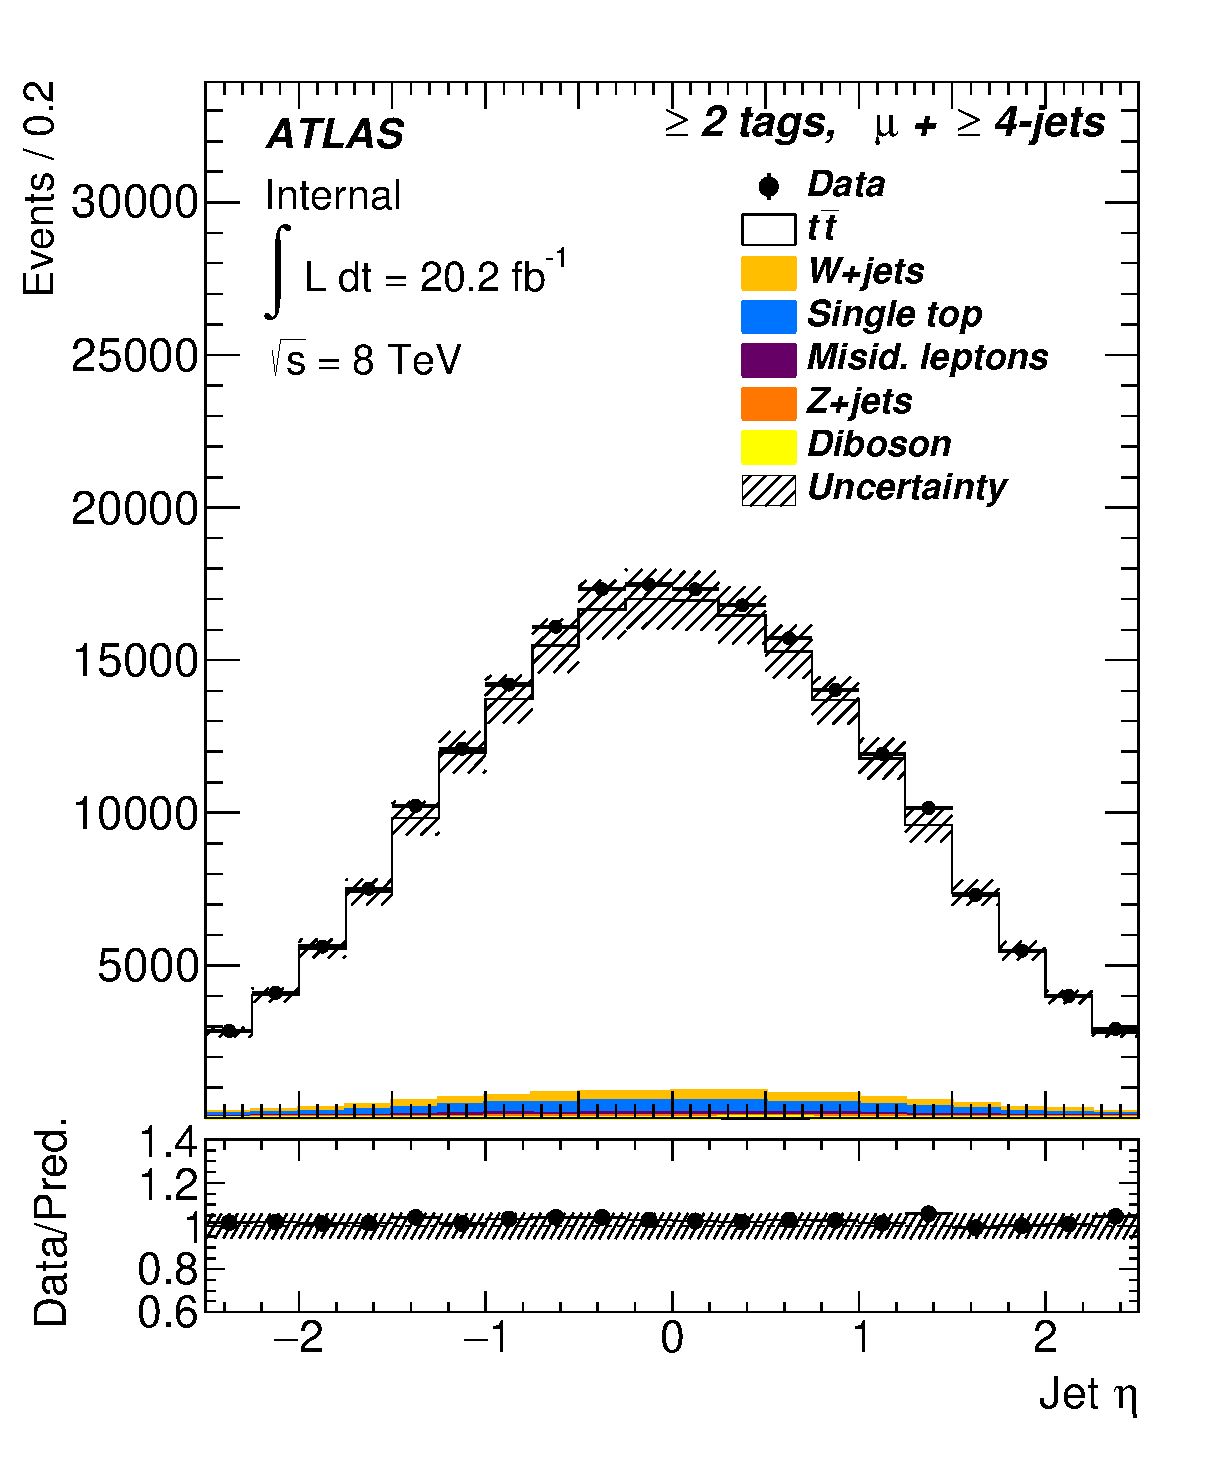
\includegraphics[height=65mm]{chapters/whel/figures/control_Plots2/bTag_2incl/JetEta_mu}\\
		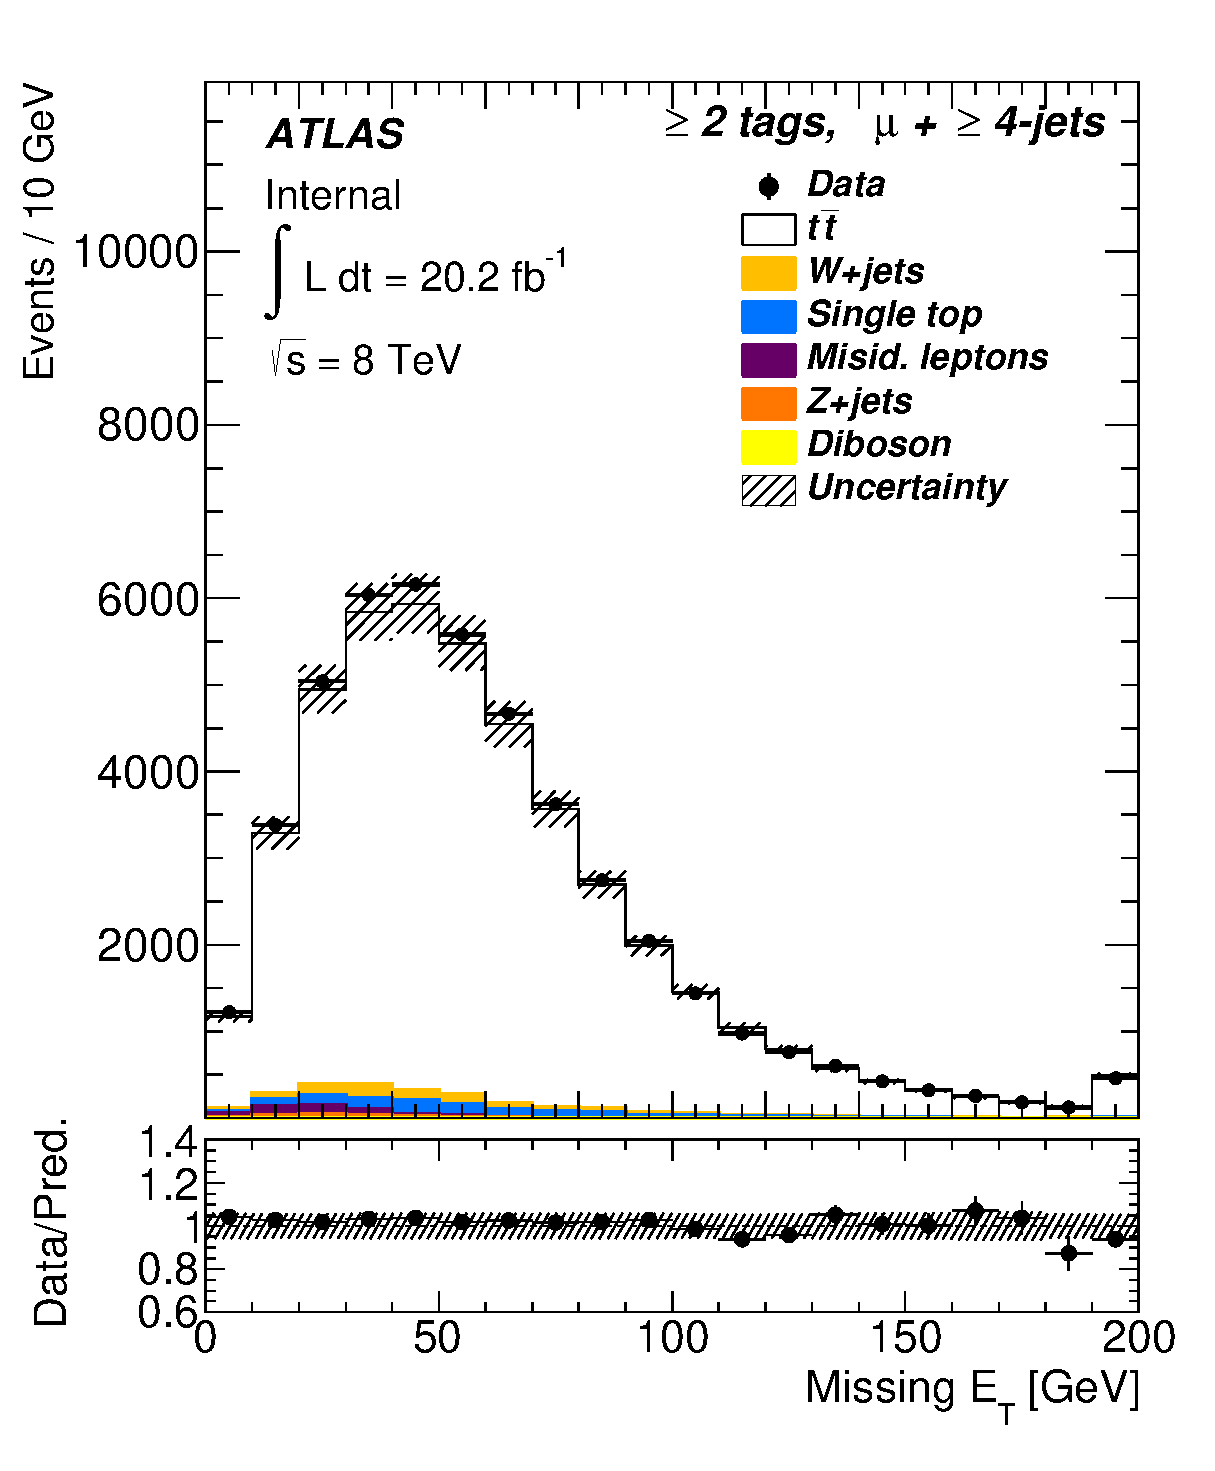
\includegraphics[height=65mm]{chapters/whel/figures/control_Plots2/bTag_2incl/MissingEt_mu}
        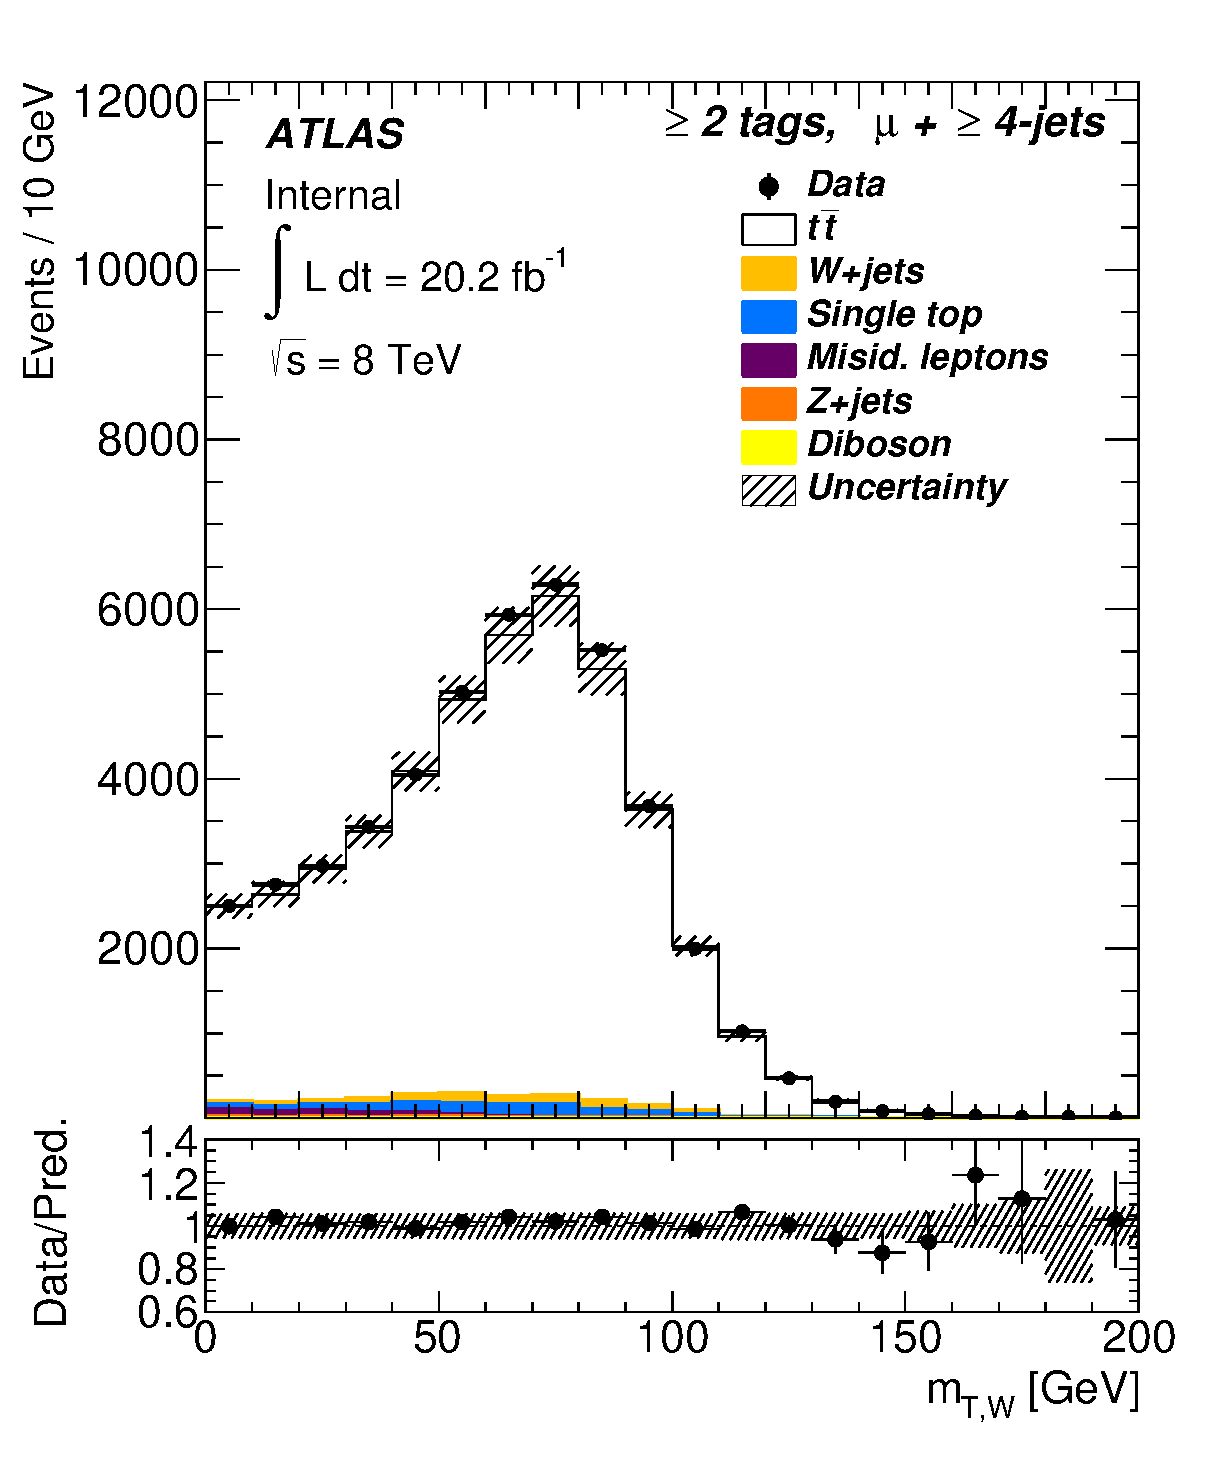
\includegraphics[height=65mm]{chapters/whel/figures/control_Plots2/bTag_2incl/TransverseMass_mu}
	\caption{Plots showing data/MC agreement after event selection for reconstructed objects (lepton, jets, neutrino) in the 2 inclusive \bt tag, muon region. The shaded bands represent the Monte Carlo statistical uncertainties.}
	\label{fig:control_plots_mu_2incl}
	\end{center}
	\end{figure}

\begin{figure}[!hb]
  \begin{center}
    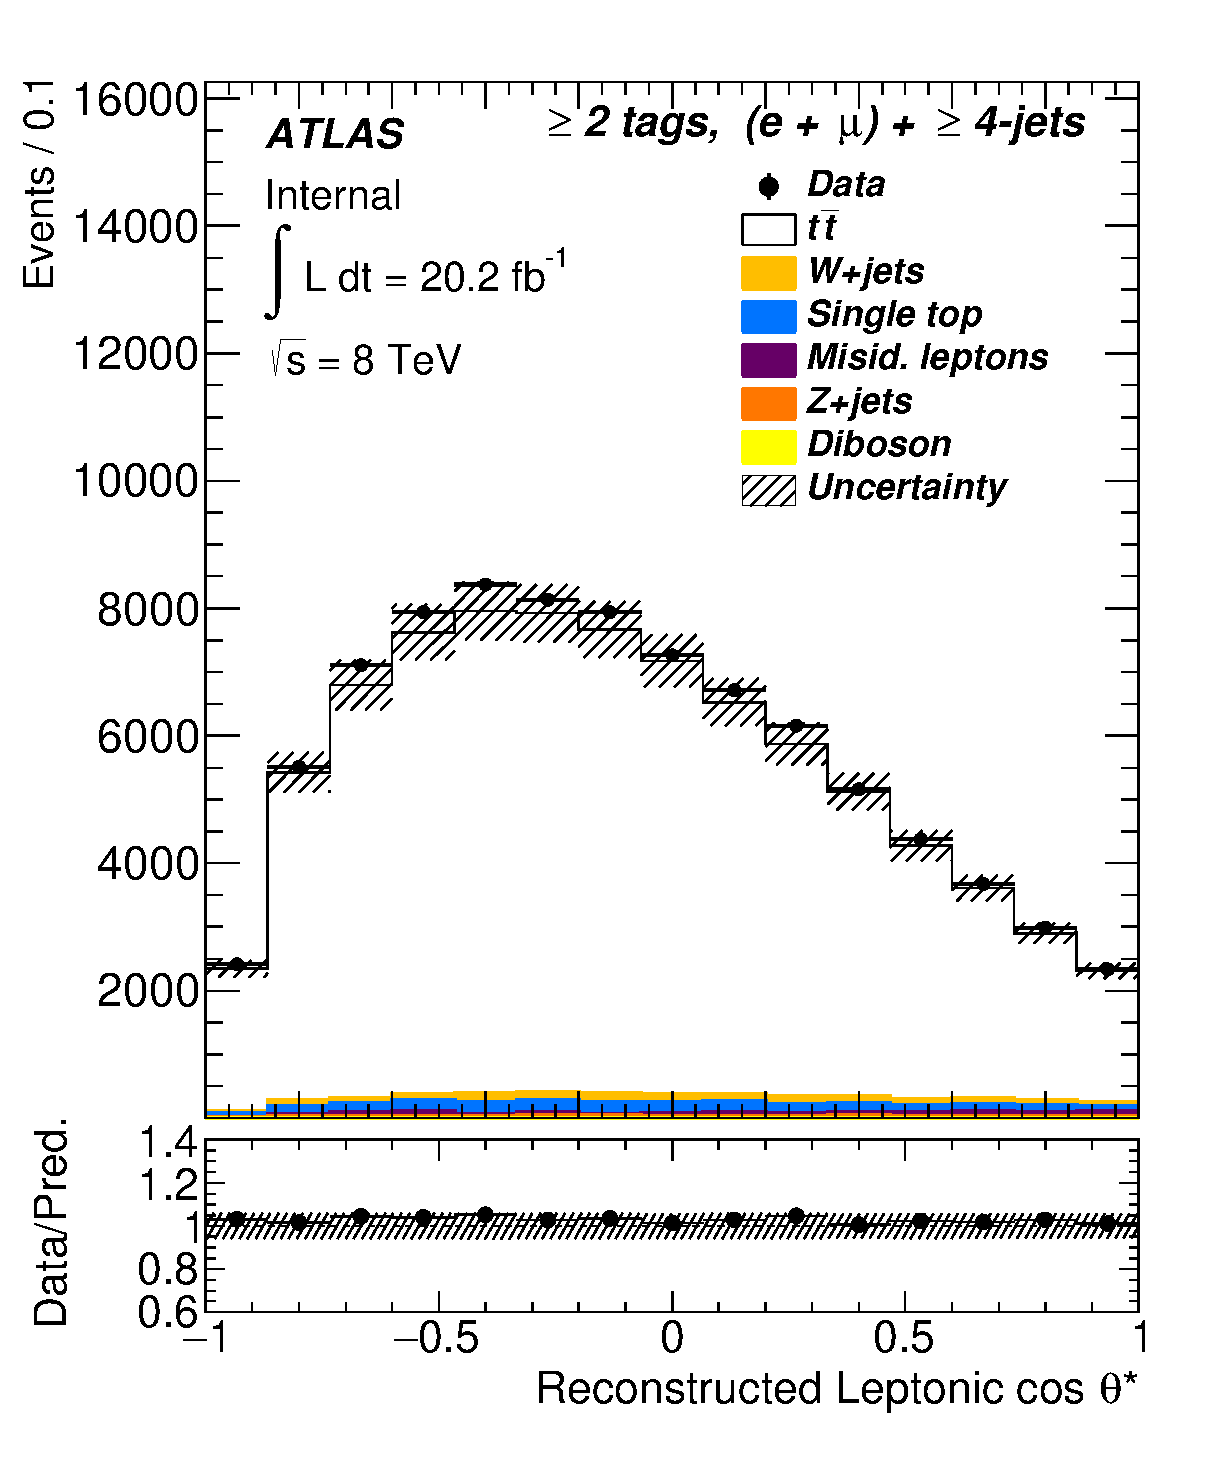
\includegraphics[height=65mm]{chapters/whel/figures/control_Plots2/elmu_2incl_LH48/CosTheta_reco_lep_elmu}
    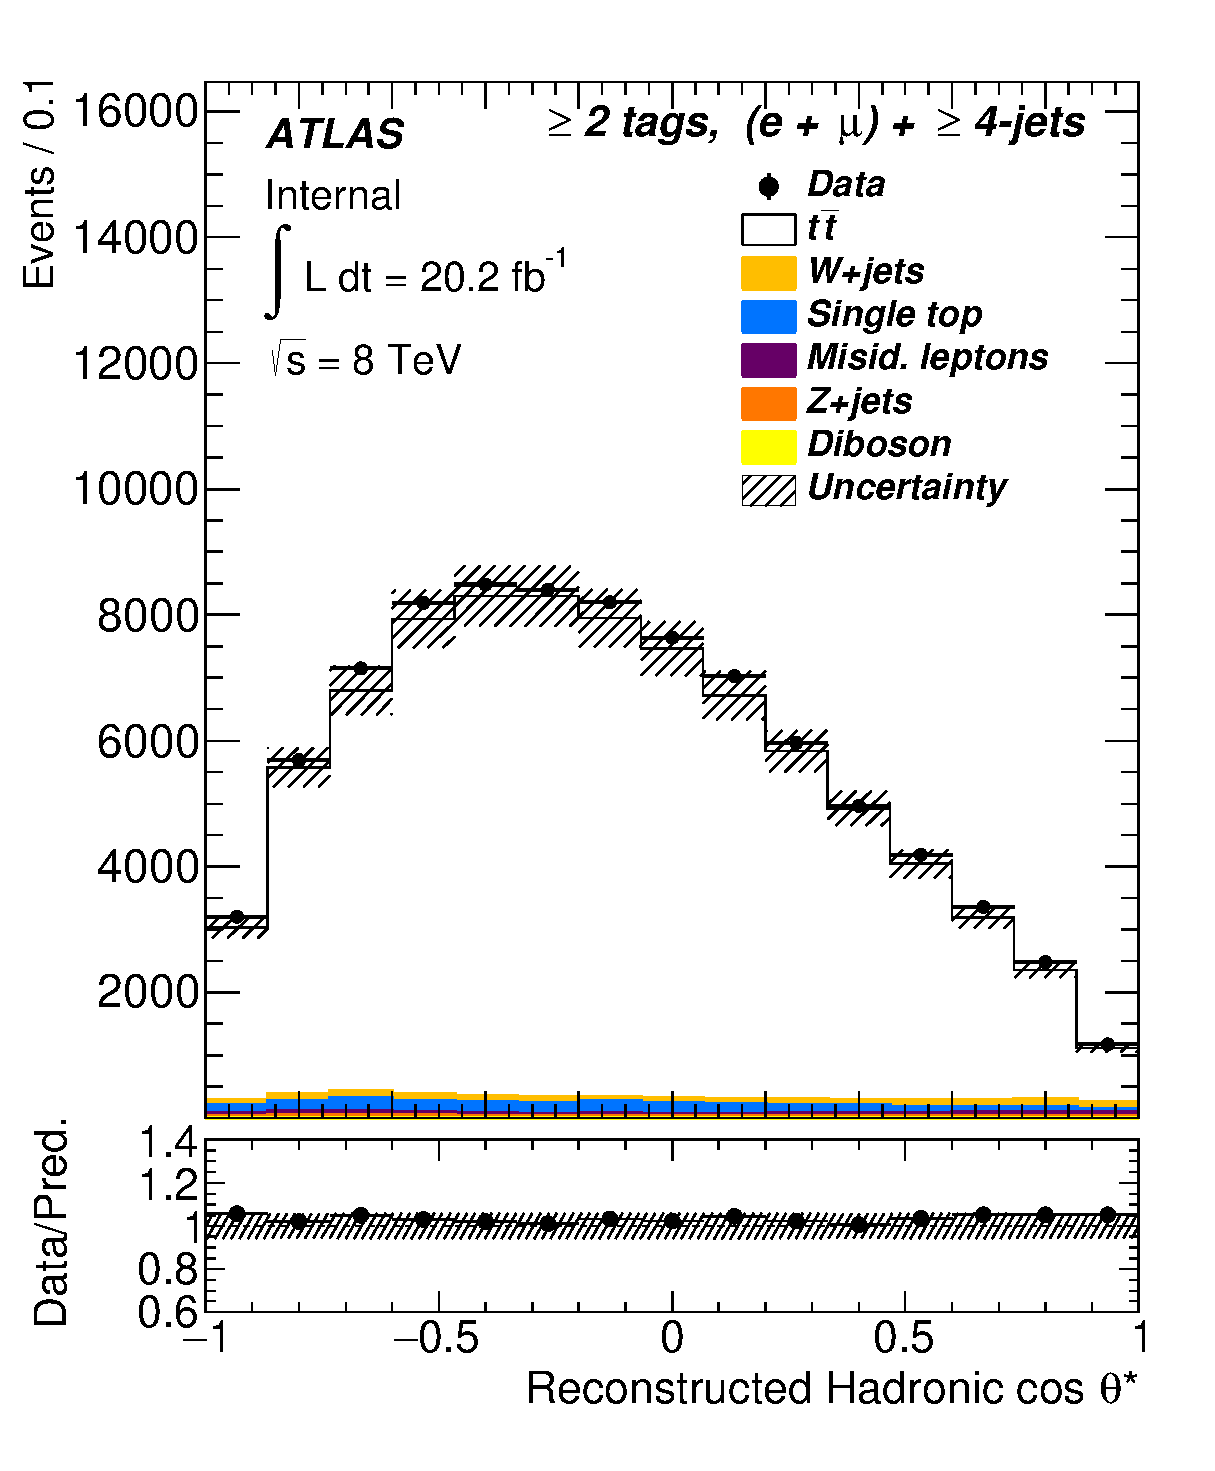
\includegraphics[height=65mm]{chapters/whel/figures/control_Plots2/elmu_2incl_LH48/CosTheta_reco_had_elmu}\\
    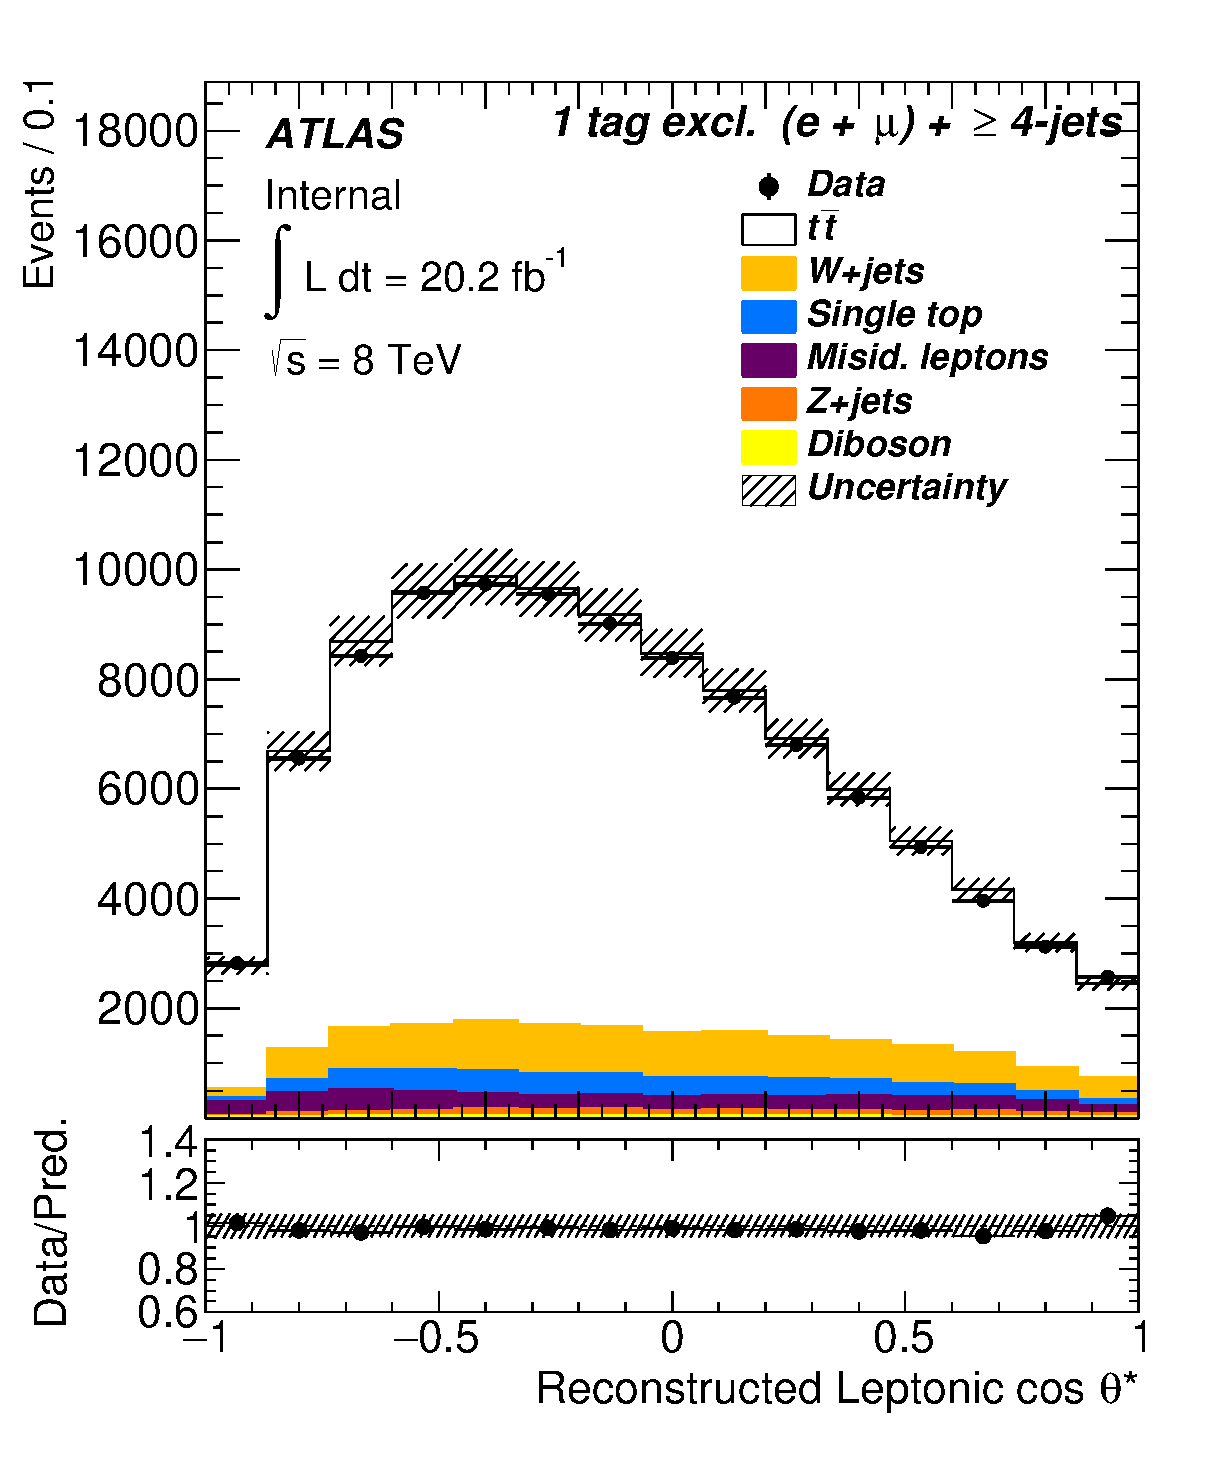
\includegraphics[height=65mm]{chapters/whel/figures/control_Plots2/elmu_1excl_LH48/CosTheta_reco_lep_elmu}
    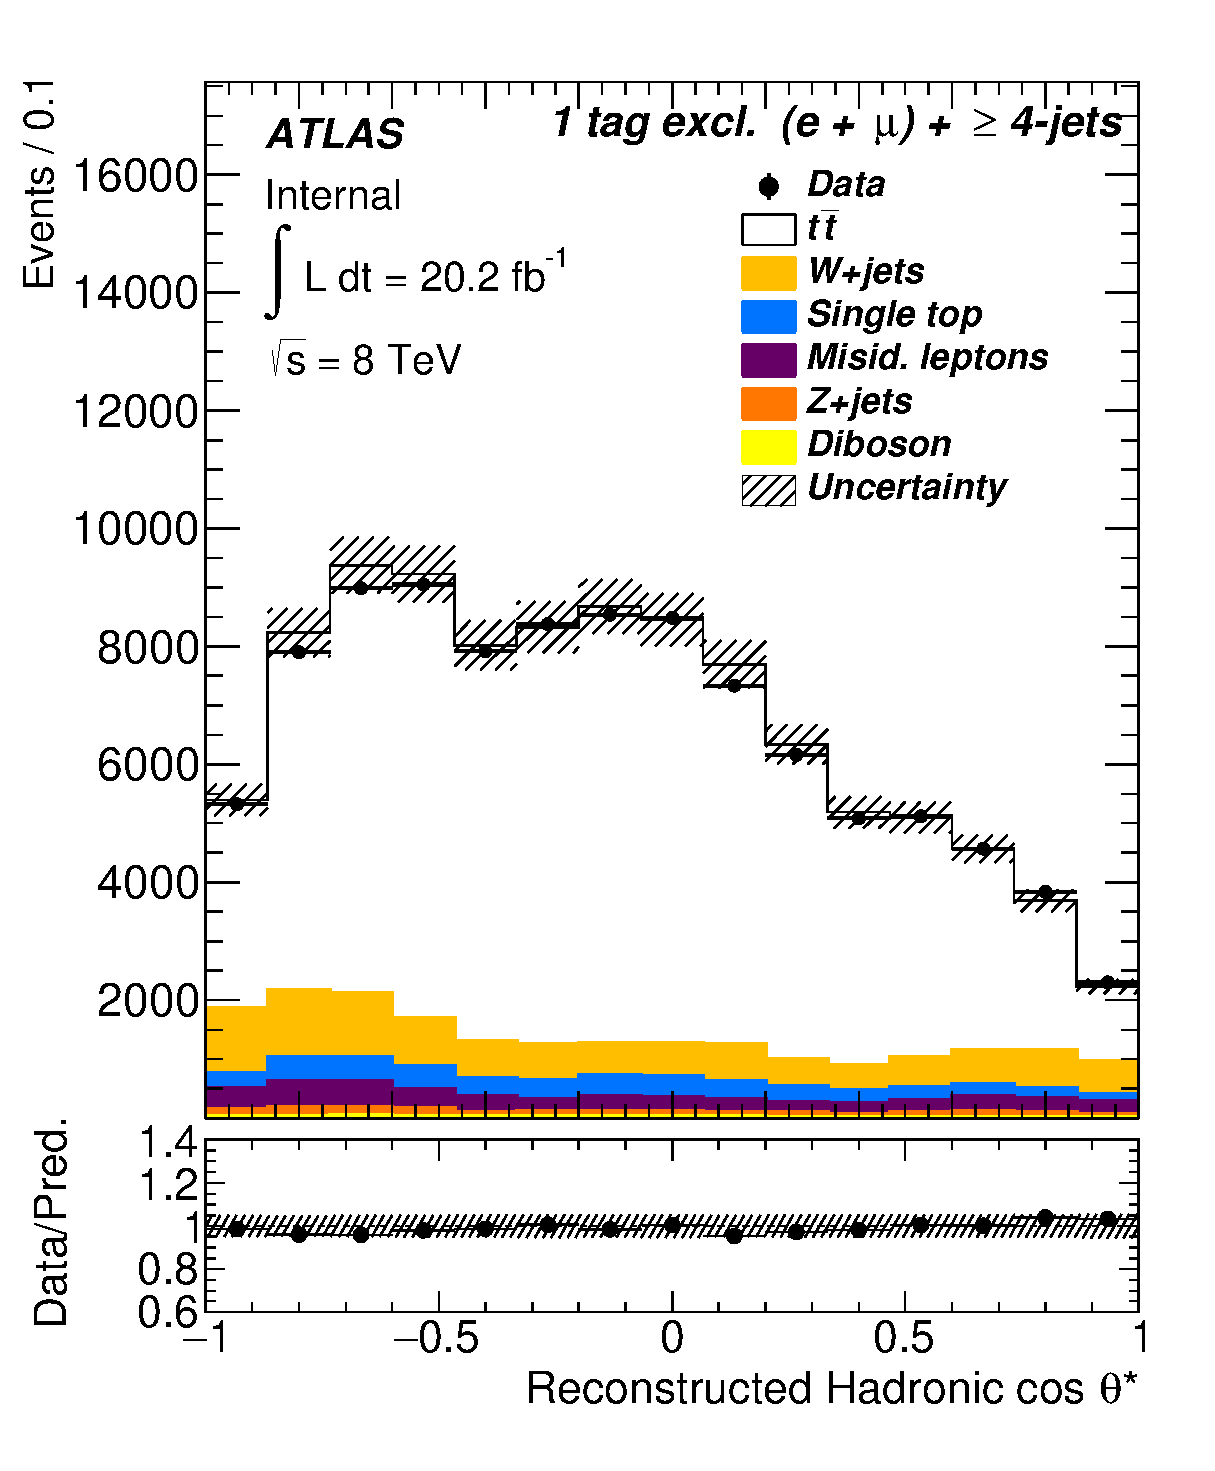
\includegraphics[height=65mm]{chapters/whel/figures/control_Plots2/elmu_1excl_LH48/CosTheta_reco_had_elmu}
    \caption{Plots showing data/MC agreement after event selection and after the likelihood cut for leptonic and hadronic $\cos\theta^*$ in the 2 inclusive \bt tag (top) and 1 exclusive \bt tag (bottom) region. All plots show merged electron+muon data and Monte Carlo. The shaded bands represent the Monte Carlo statistical uncertainties.}
    \label{fig:control_plots_costheta}
  \end{center}
\end{figure}
\clearpage
%-------------------------------------------------------
%-------------- Bkg + Signal Modelling -----------------
%-------------------------------------------------------------------------------
\section{Background and Signal Modeling}
\label{sec:backgroundAndSignalModelling}
%-------------------------------------------------------------------------------
After event selection, the largest remaining background comes from the production of a \w boson in association with
jets ($W$+jets) with multi-jet QCD production contributing to a lesser extent. Small contributions arise from single top quark, $Z$+jets and diboson ($WW,WZ,ZZ$) production. The absolute yield of all considered backgrounds rises in the 1 exclusive \bt tag region while the contributions from single top and $W$+jets backgrounds also increase relatively with respect to the other backgrounds.

Multi-jet events contribute to the selected sample via the mis-identification of a jet or a photon as an electron or the presence of a non-prompt lepton, e.g.~from a semileptonic \bt- or $c$-hadron decay, and the corresponding yield is estimated using a data-driven matrix method ~\cite{ttbar_3pb}.
%The \w+jets background is estimated using simulation. %The heavy flavor component of the \w+jets background is determined from data and the overall yield normalized using a data-driven charge asymmetry method.

%Details on the estimation of the multijet background are given in Sect.~\ref{sec:DataDrivenBackground}.
%Yields from the remaining backgrounds (as well as the \ttbar signal) are determined from Monte Carlo simulations normalised to their appropriate theoretical cross sections.

%In the di-lepton channel backgrounds other than $t\bar{t}$+jets production
%arise mainly from $Z$+jets production and from
%the \w+jets and \ttbar\ production with a single lepton in the final state.
%The latter contain non-prompt leptons that pass lepton isolation
%requirement or misidentified leptons arising from jets. In this analysis
%their yield is estimated using simulation as described in
%Sect.~\ref{sec:DataDrivenBackground}.
%$Z$+jets background is estimated from simulation corrected for the discrepancy
%of the $Z$ \pt\ spectrum between data and simulation. Heavy flavor component of
%$Z$+jets background is also determined from data (see Appendix~\ref{sec:Vjets}).

Small background contributions coming from single top quark, $Z$+jets and diboson production are estimated from simulation and normalized to their theoretical cross sections.

Samples of $W/Z$+jets events at 8 TeV are generated using the {\sc Alpgen v2.14}~\cite{alpgen} leading-order (LO) generator and the {\sc CTEQ6L1} PDF set~\cite{cteq6}. Parton shower and fragmentation are modeled with {\sc Pythia} 6.425~\cite{Sjostrand:2006za} for $W$+jets and $Z$+jets production. To avoid double-counting of partonic configurations generated by both the matrix-element calculation and the parton-shower evolution, a parton-jet matching scheme (``MLM matching")~\cite{mlm} is employed. Since final states with hadronic $Z$ decays of $WZ$ are missing in {\sc Alpgen}+{\sc Herwig} production, {\sc Sherpa} samples generated with massive $b$ and $c$ quarks (i.e. $b$ and $c$ quark masses are set to their PDG values in the matrix element calculation as opposed to being set massless) are used for these decay modes.

The \w+jets samples are generated with up to five additional partons, separately for $W$+light jets, $Wb\bar{b}$+jets, $Wc\bar{c}$+jets, and $Wc$+jets. The overlap between $Wq\bar{q}$ ($q=b,c$) events generated from the matrix element calculation and those generated from parton-shower evolution in the $W$+light jet samples is removed by using the angular separation between the extra heavy quarks: if $\Delta R(q,\bar{q})>0.4$, the matrix-element prediction is used, otherwise the parton-shower prediction is used. The $W$+jets background is normalized using data-driven calibration factors which take into account the charge of the lepton and heavy flavor components of the associated jets. The method and factors were derived in the 8 TeV ATLAS \ttbar charge asymmetry analysis ~\cite{Juste:1647184}.

The $Z$+jets background is generated using the {\sc Alpgen v2.14}~\cite{alpgen} leading-order (LO) generator with up to five additional partons separated by different parton flavors and is normalized to the inclusive NNLO theoretical cross section~\cite{vjetsxs}.

The $WW/WZ/ZZ$+jets samples are generated using {\sc Sherpa} with up to three additional partons in the hard process and are normalized to their NLO theoretical cross sections~\cite{dibosonxs}. Heavy flavor quarks (\bt and $c$) are treated as massive in the matrix element calculation and generation of all diboson samples.

The $t\bar{t}$ sample is generated using {\sc Powheg} NLO generator~\cite{powheg,powbox1,powbox2} with the {\sc CT10} PDF set assuming a top quark mass of $172.5\gev$ and setting the $h_{damp}$ factor (the parameter responsible for high \pt radiation damping in the {\sc POWHEG-BOX} generator) equal to the top quark mass. {\sc Powheg} is interfaced to {\sc Pythia} 6.425~\cite{Sjostrand:2006za} with the {\sc CTEQ61L} set of parton distribution functions and Perugia2011C underlying event tune. The sample is normalized to the theoretical calculation performed at next-to-next-to leading order (NNLO) in QCD including resummation of next-to-next-to-leading logarithmic (NNLL) soft gluon terms with top++2.0~\cite{ref:xs1,ref:xs2,ref:xs3,ref:xs4,ref:xs5,Czakon:2011xx}. At 8 TeV, the \ttbar cross-section is calculated to be $253^{+15}_{-16}$~pb. 

Effects due to PDF variations, choice of $\alpha_S$, and the input top quark mass are taken as systematic uncertainties. The PDF and $\alpha_S$ uncertainties are calculated using the PDF4LHC prescription~\cite{ref:pdf4lhc} with the MSTW2008 68\% CL NNLO~\cite{mstw1,mstw2}, CT10 NNLO~\cite{Lai:2010vv,ct102} and NNPDF2.3 5f FFN~\cite{nnpdf} PDF sets added in quadrature to the scale uncertainty. Unlike multi-leg generators, {\sc Powheg} is expected to describe jet multiplicity properly only for \ttbar accompanied by up to two jets. Nevertheless when interfaced with {\sc Pythia}, {\sc Powheg} provides good description of jet multiplicity in data up to much higher jet multiplicities and reproduces the associated heavy flavor fraction in \ttbar production despite the fact that heavy flavor component originates only from the parton shower~\cite{Aad:2015gra}. %The  {\sc Powheg}+{\sc Pythia} \ttbar sample is re-weighted as a function of top quark \pt to remove discrepancies in the high top quark and \ttbar \pt regions as observed in data~\cite{topdiff_7TEV}. The details of the correction procedure and associated systematic uncertainties are described in Appendix~\ref{app:topmodel}.

%A detailed study comparing the $t\bar{t}$ sample generated using {\sc Powheg} NLO generator~\cite{powheg,powbox1,powbox2}
%with the {\sc CT10} PDF set assuming top quark mass of $172.5\gev$ and $h_{damp}$ factor set to infinity with the default signal sample mentioned above is presented in Appendix \ref{app:hdamp_comparison}.

Samples of single top quark backgrounds corresponding to the $s$-channel, $t$-channel and $Wt$ production mechanisms are generated with {\sc Powheg}~\cite{powheg,powbox1,powbox2} using the {\sc CT10} PDF set~\cite{ct10}.  In the case of the $Wt$-channel, the nominal sample uses a diagram removal approach to handle the interference arising at NLO. All samples are interfaced to {\sc Pythia} 6.425~\cite{Sjostrand:2006za} with the {\sc CTEQ61L} set of parton distribution functions and Perugia2011C underlying event tune. Overlaps between the \ttbar\ and $Wt$ final states are removed~\cite{mcatnlo_2}. The single top quark samples are normalized to the approximate NNLO theoretical cross sections~\cite{stopxs,stopxs_2} using the {\sc MSTW2008} NNLO PDF set.

All event generators using {\sc Herwig} are also interfaced to {\sc Jimmy} v4.31~\cite{jimmy} to simulate the underlying event. All simulated samples utilize {\sc Photos 2.15}~\cite{PhotosPaper} to simulate photon radiation and {\sc Tauola 1.20}~\cite{TauolaPaper} to simulate $\tau$ decays. All simulated samples (including the \ttbar signal) include multiple $pp$ interactions and are processed through a simulation~\cite{Aad:2010ah} of the detector geometry and response using {\sc Geant4}~\cite{Agostinelli:2002hh}. All simulated samples are processed through the same reconstruction software as the data. Simulated events are
corrected so that the object identification efficiencies, energy scales and energy resolutions match those determined in data control samples.

Table~\ref{tab:NBparam} provides a summary of basic parameters of the MC samples used in the analysis. %Full list of MC samples is available in Appendix \ref{app:mcSamples}.

\begin{table}
\small
\centering     % 1 2 3 4 5                                                                                                                                                                                     
\begin{tabular}{|c|c|c|c|c|}
\hline
Sample & Generator & PDF & Shower & Normalization \\
\hline
%\tth    & HELAC-Oneloop  & CT10  & Pythia $8.1$ & NLO\\
\ttbar + jets &  Powheg & CT10 & Pythia $6.425$ & NNLO+NNLL~\cite{ttbarNorm1,Frixione:2007vw,ttbarNorm3}\\
\w + jets & Alpgen & CTEQ$6$L$1$ & Pythia $6.426$ & 8 TeV charge asymmetry CAs~\cite{Juste:1647184}\\
$Z$ + jets & Alpgen & CTEQ$6$L$1$ & Pythia $6.426$ & NLO~\cite{ZjetsNorm} \\
Single top (s-channel, Wt) & Powheg & CT10 & Pythia $6.426$ & aNNLO~\cite{Kidonakis:2011wy, Kidonakis:2010ux,singleTopNorm3}\\
Single top (t-channel) & Powheg & CT10 & Pythia $6.427$ & aNNLO~\cite{Kidonakis:2011wy, Kidonakis:2010ux,singleTopNorm3}\\
Diboson & Sherpa & CT10 & Sherpa  &  NLO~\cite{dibosonNorm} \\
\hline
\end{tabular}
\caption{A summary of basic generator parameters used to simulate various
processes}
\label{tab:NBparam}
\end{table}

%-------------------------------------------------------
%-------------- Event Reconstruction -------------------
%-------------------------------------------------------------------------------
\section{Event Reconstruction}
\label{sec:eventReconstruction}
%-------------------------------------------------------------------------------
%\subsection{Lepton+jets Channel} 
A kinematic fitting technique is used to reconstruct candidate events passing basic selection requirements and identify optimal jet assignments. The following section details the methodology of the kinematic fit as well as extensions that use information beyond object kinematics in order to produce the final jet assignments. A number of different configurations are studied in order to determine the optimal setup to extract the helicity fractions.
\subsection{Kinematic Fitting} 
The events are reconstructed using a kinematic likelihood code package (KLFitter) \cite{klfitter} which makes use of the Bayesian Analysis Toolkit (BAT) \cite{Caldwell:2008fw}. KLFitter takes an input model (e.g., \ttbar decay) and mass constraints (\mt, \mW) on composite objects built from the input leptons, \met, and jets to map the input particles to leading order partons/leptons from the \ttbar decay. Transfer functions are used to float the measured energies of the jets and lepton within detector resolutions. Separate transfer functions are defined for jets/leptons/\met in different $\eta$ ranges, but the measured angles themselves are assumed to be correctly reconstructed. The final two and three-body masses are evaluated with Breit-Wigner PDFs using \mt = 172.5 GeV and \mW = 80.2 GeV. The Breit-Wigner widths are set to $\Gamma_t=1.33$ GeV and $\Gamma_W=2.1$ GeV for the top quark and $W$ boson respectively. The final expression for likelihood, $\mathscr{L}$, is then expressed as 

\begin{eqnarray}
&& \mathscr{L}=BW(m_{q_1q_2q_3}| \mt\Gamma_{t})\cdot BW(m_{q_1q_2}| \mW\Gamma_{W})\cdot BW(m_{q_4\ell\nu}| \mt\Gamma_{t})\cdot BW(m_{\ell\nu} | \mW\Gamma_{W}) \nonumber \\
&& \prod\limits_{i=1}^4 W_{jet}(E_{i}^{meas}|E_{i})\cdot W_{\ell}(E_{\ell}^{meas}|E_{\ell})\cdot W_{miss}(E_{x}^{miss}|p_{x}^{\nu})\cdot W_{miss}(E_{y}^{miss}|p_{y}^{\nu}) .
\label{eq:KLF}
\end{eqnarray}
where $q_i$ ($i=1,2,3,4$) are the labels for the four jets used in the calculation, $W_{i}(E_{x}^{meas}|E_{i})$ are the transfer functions, $E_{x}^{meas}$ is the measured energy of object $x$, $E_{i}$ is the 'true' energy of the reconstructed parton $i$, and the $BW(m_{ij(k)}| m_{Y}\Gamma_{Y})$ are the Breit-Wigner functions used to evaluate the masses of composite reconstructed particles with respect to the mass and width of particle $Y$. 

Section \ref{sec:TF} provides an in-depth discussion about the construction and use of the transfer functions. Permuting the jets in an event through all positions in the model hypothesis yields different values for each permutation according to Eq. \ref{eq:KLF}. To increase the ability of KLFitter to correctly identify the assignments for each jet, additional information (e.g. \bt tagging, differences between types of light jets) can be used to improve the likelihood that a given permutation is correct.  This information can be used to extend the likelihood definition of Eq. \ref{eq:KLF} into an event probability. This extension is fully discussed in Sec. \ref{sec:udSep}.

After the likelihood (and/or event probability) of each permutation is calculated, the results are ordered, and the best permutation (defined as the permutation with the highest event probability) is selected for measuring the angles necessary to extract the helicity fractions. Reconstructed distributions from the leading permutation after a log likelihood cut of $> -48$ (abbreviated as `LH $> -48$' in the following) are shown in Figs \ref{fig:klfitter_control_plots_1}-\ref{fig:klfitter_control_plots_4}. The optimization and choice of the log likelihood cut is discussed in Section~\ref{sec:hadronicOptimization}. Good agreement between data and prediction is observed in all signal regions.

\begin{figure}[!h]
\begin{center}
		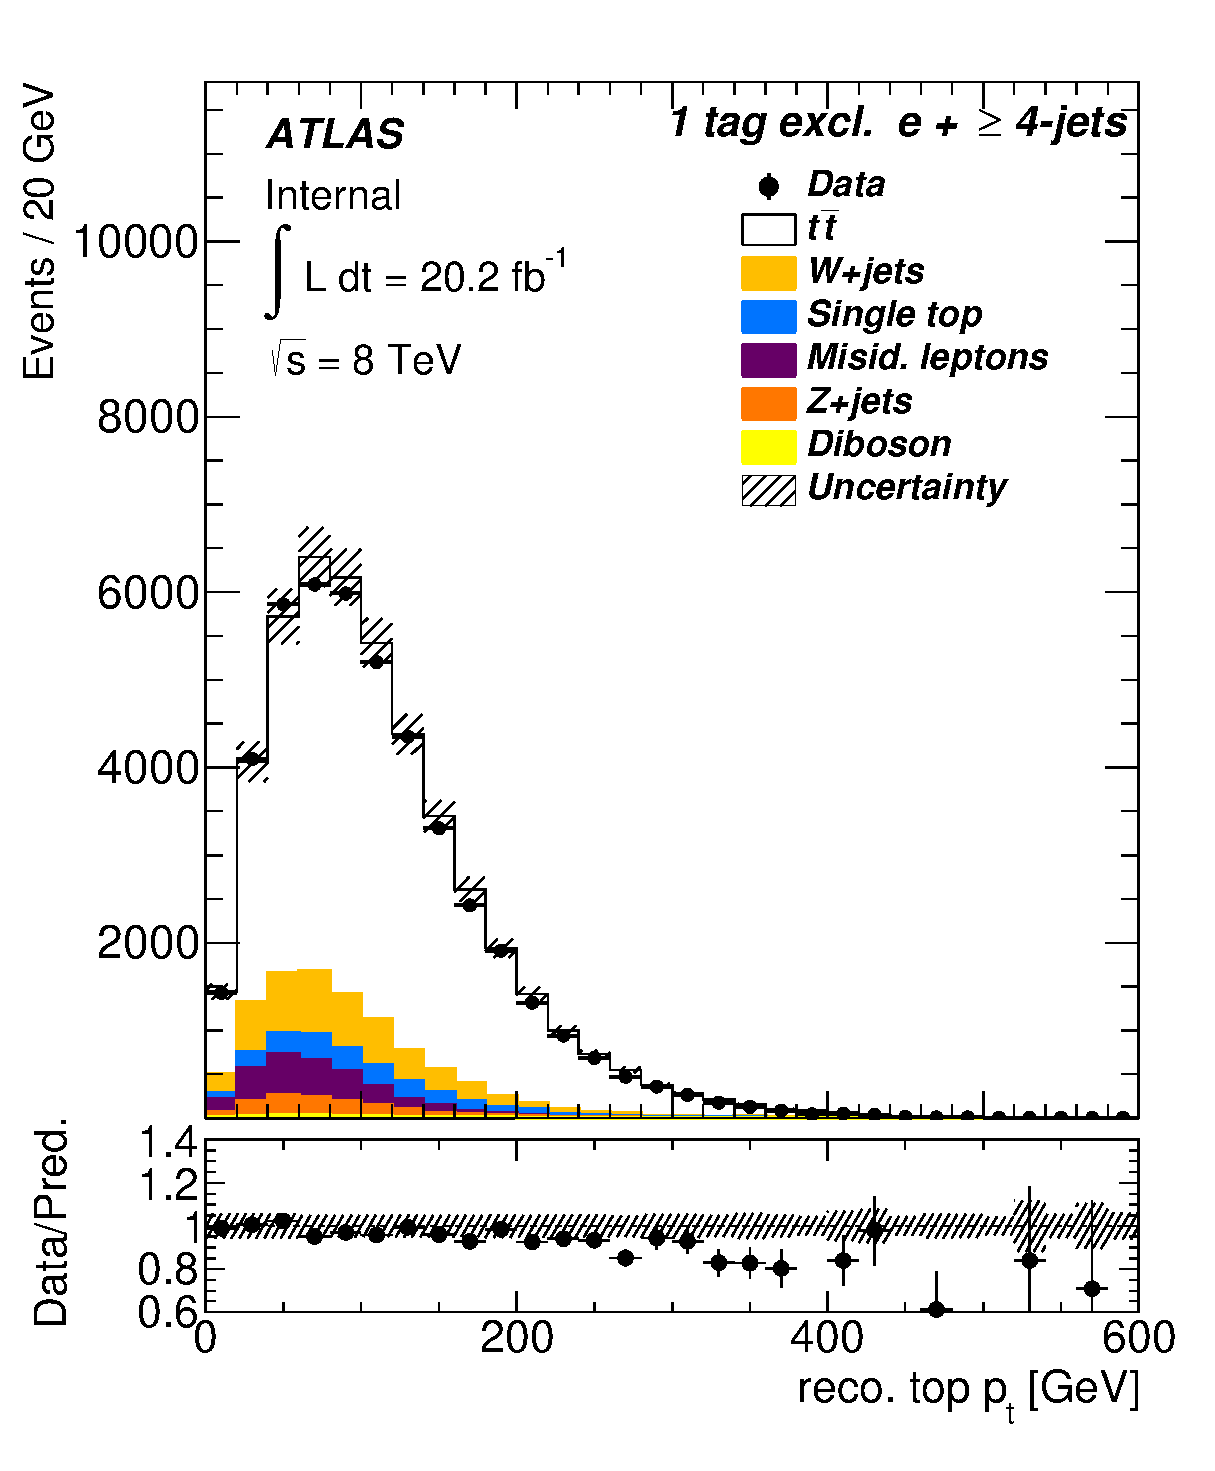
\includegraphics[height=65mm]{chapters/whel/figures/control_Plots2/bTag_1excl/reco_Top_pt_el}
		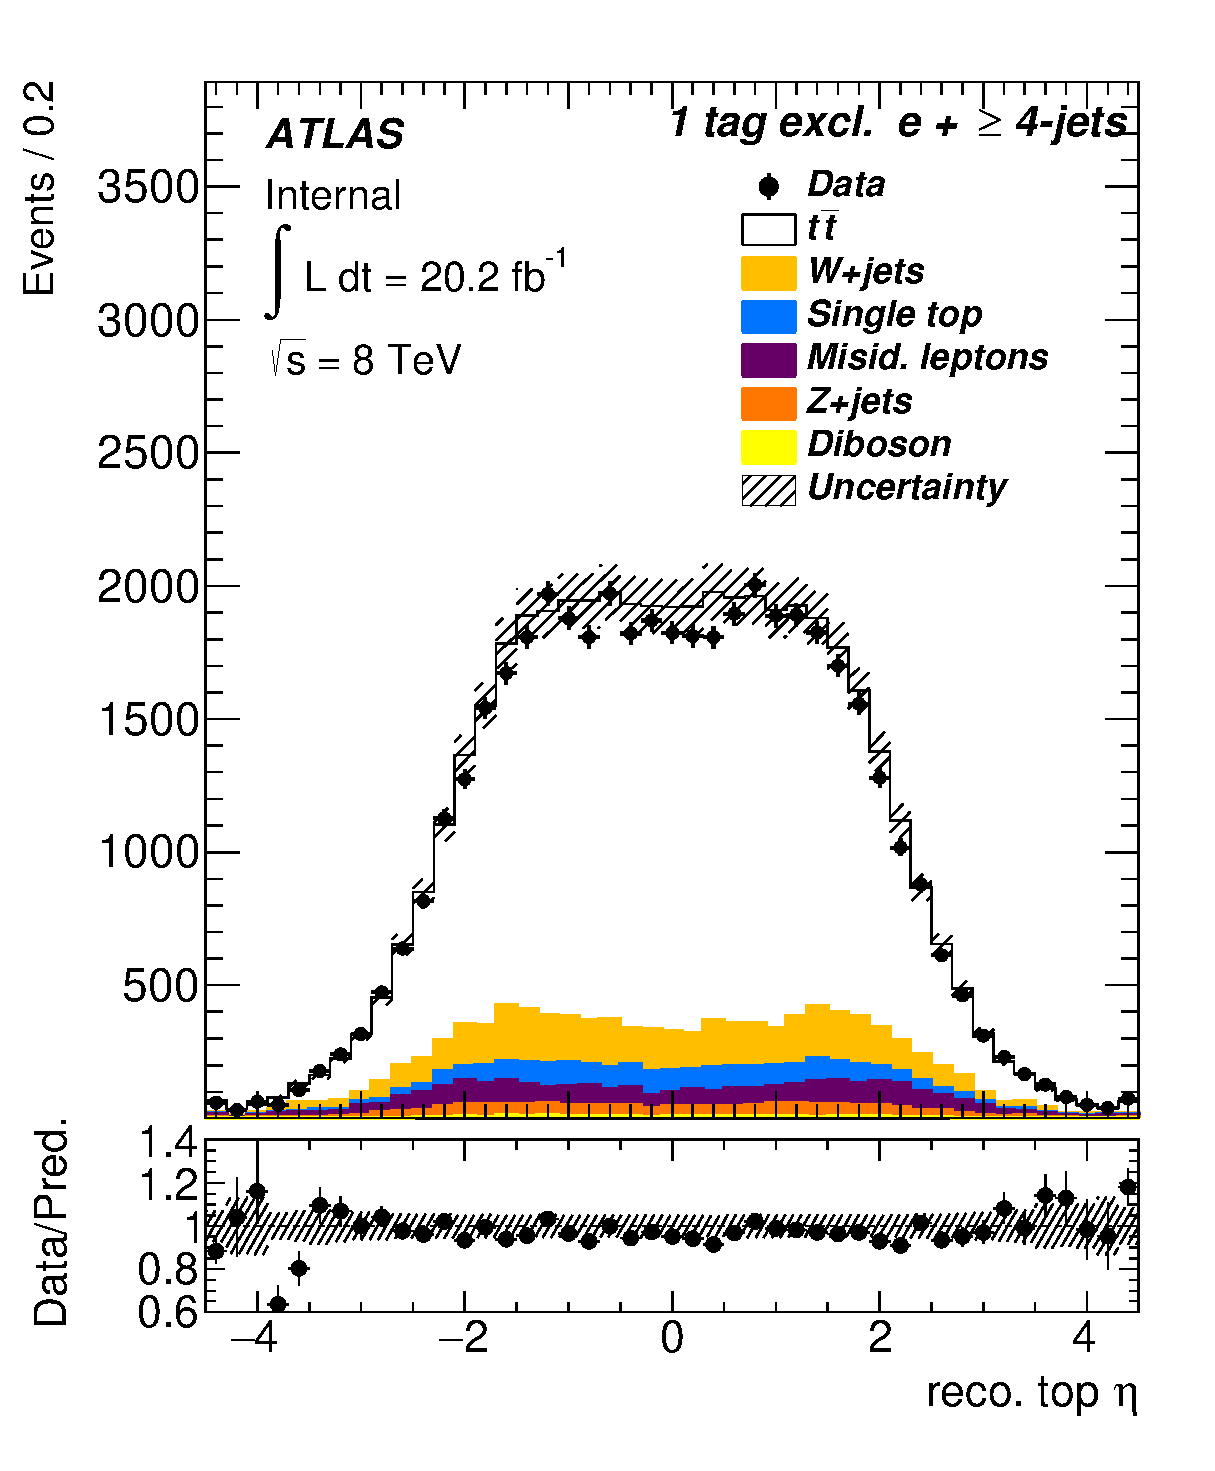
\includegraphics[height=65mm]{chapters/whel/figures/control_Plots2/bTag_1excl/reco_Top_eta_el}\\
		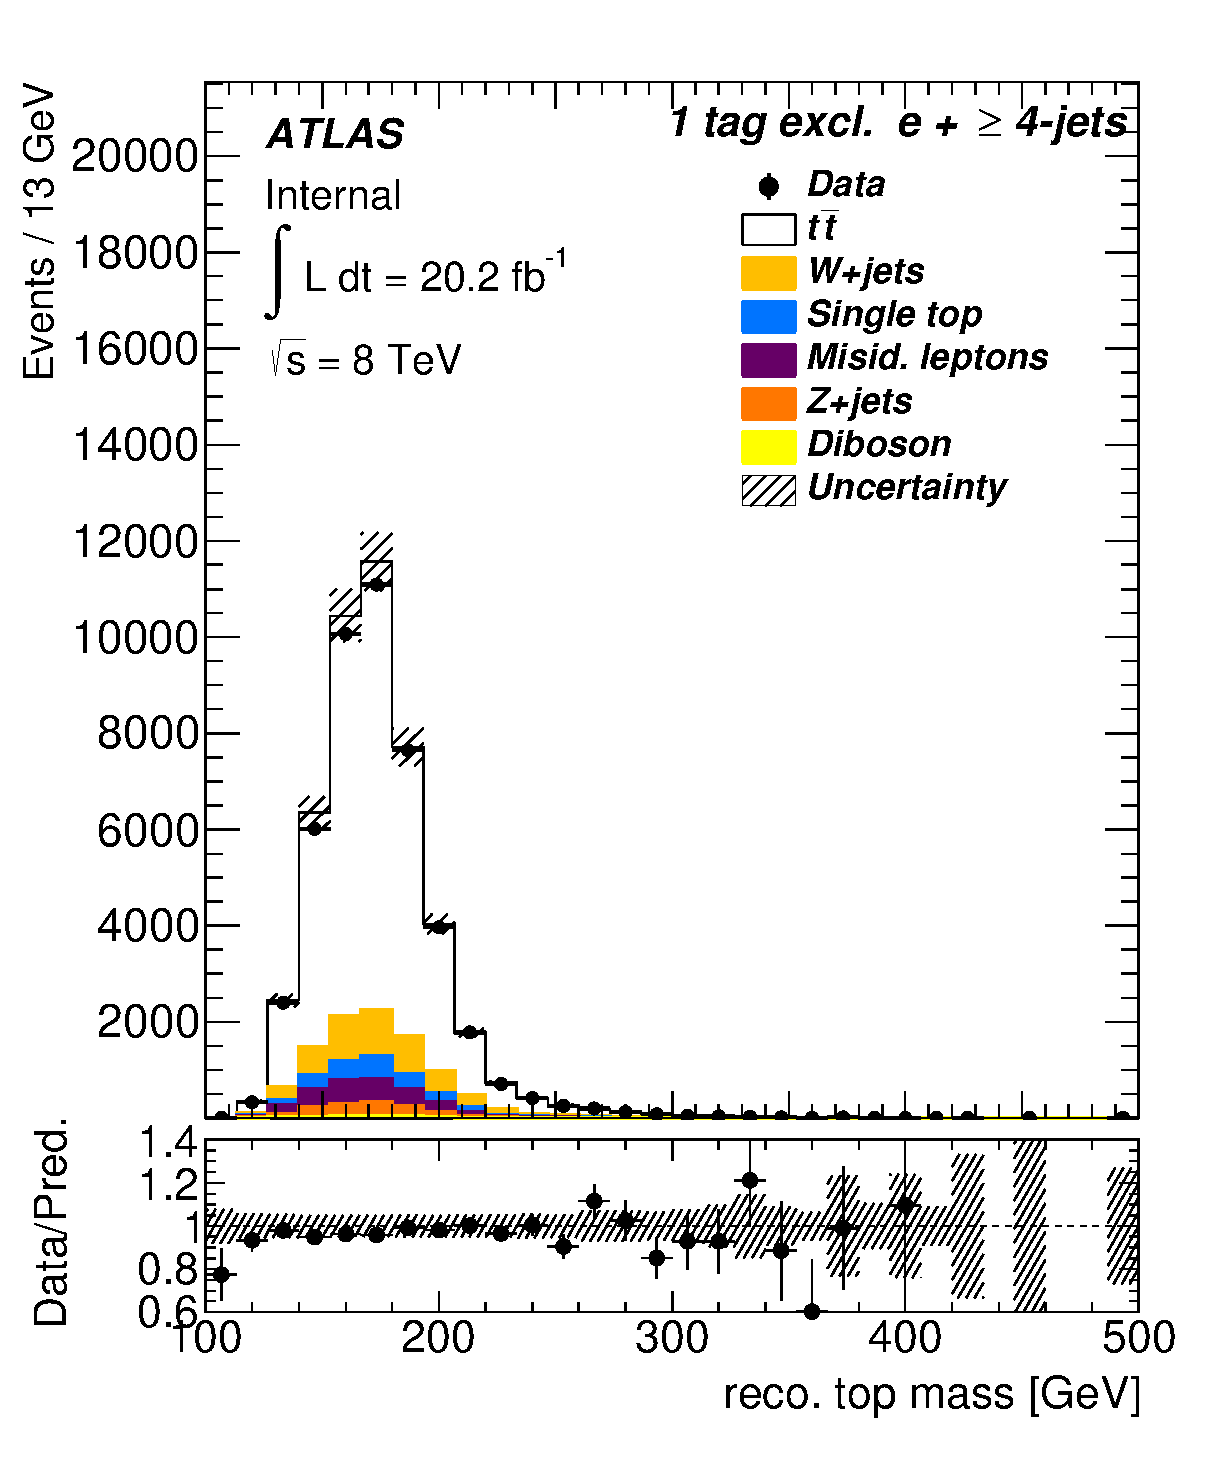
\includegraphics[height=65mm]{chapters/whel/figures/control_Plots2/bTag_1excl/reco_Top_m_el}
		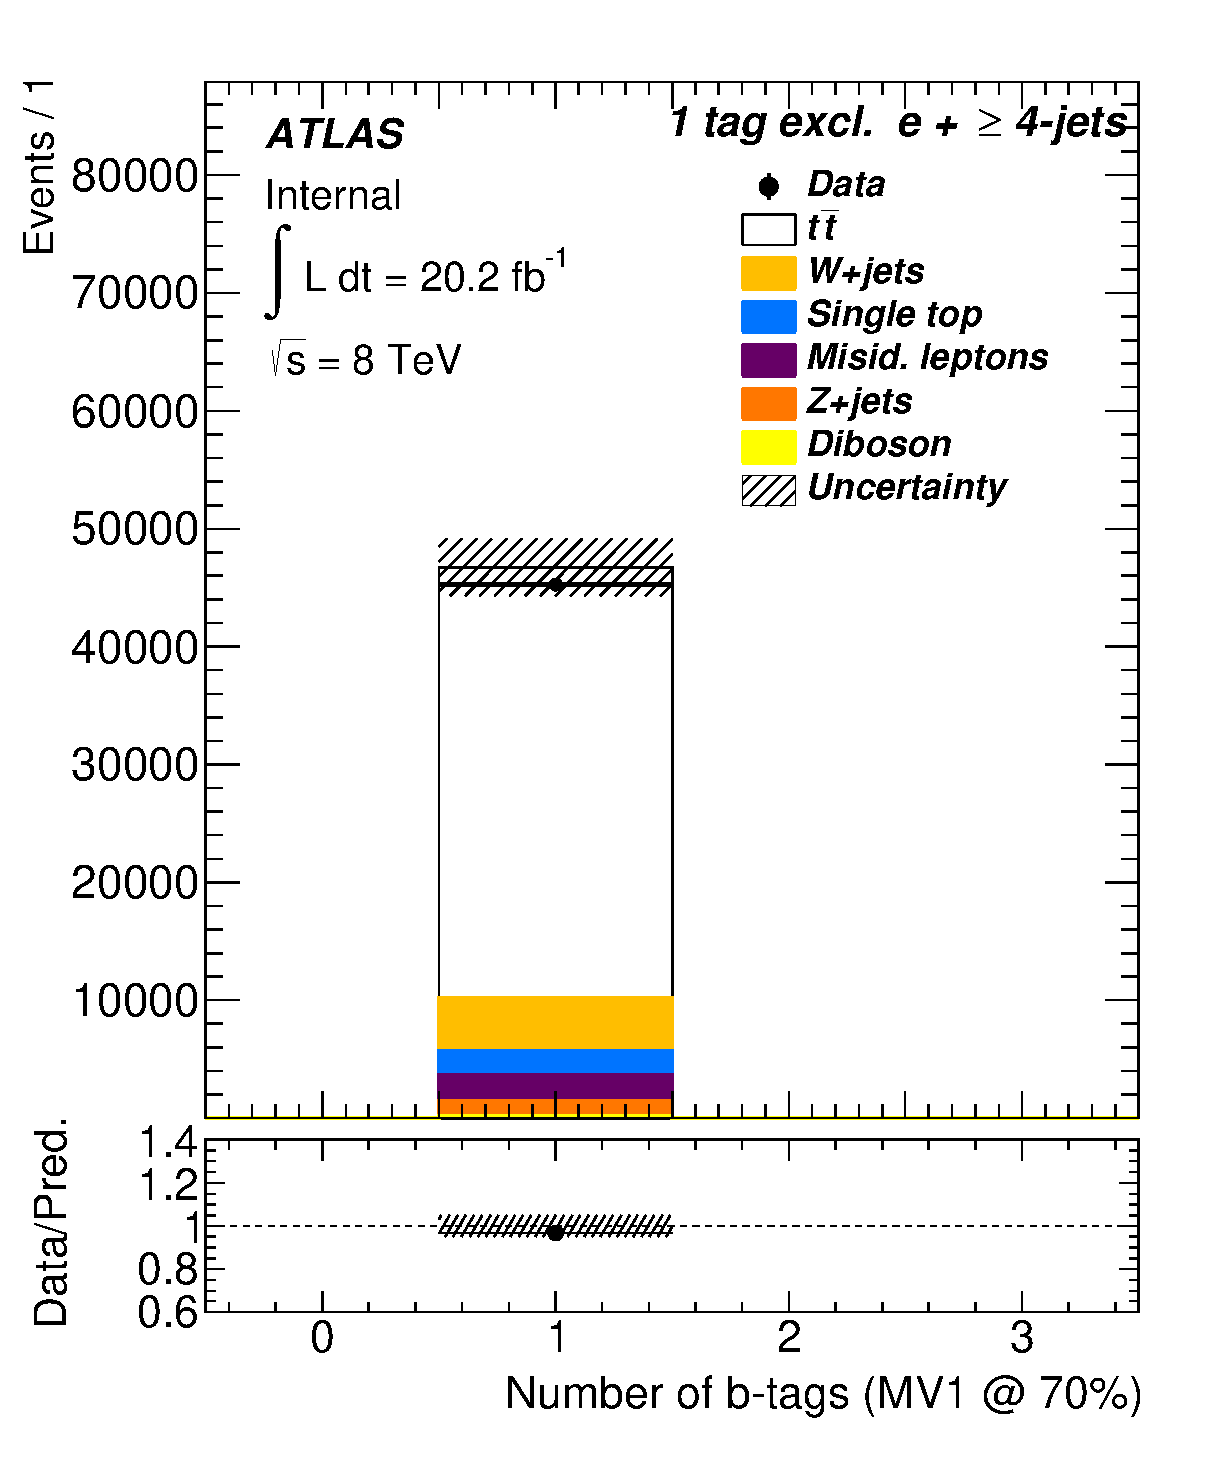
\includegraphics[height=65mm]{chapters/whel/figures/control_Plots2/bTag_1excl/NumberBtags_el}\\
		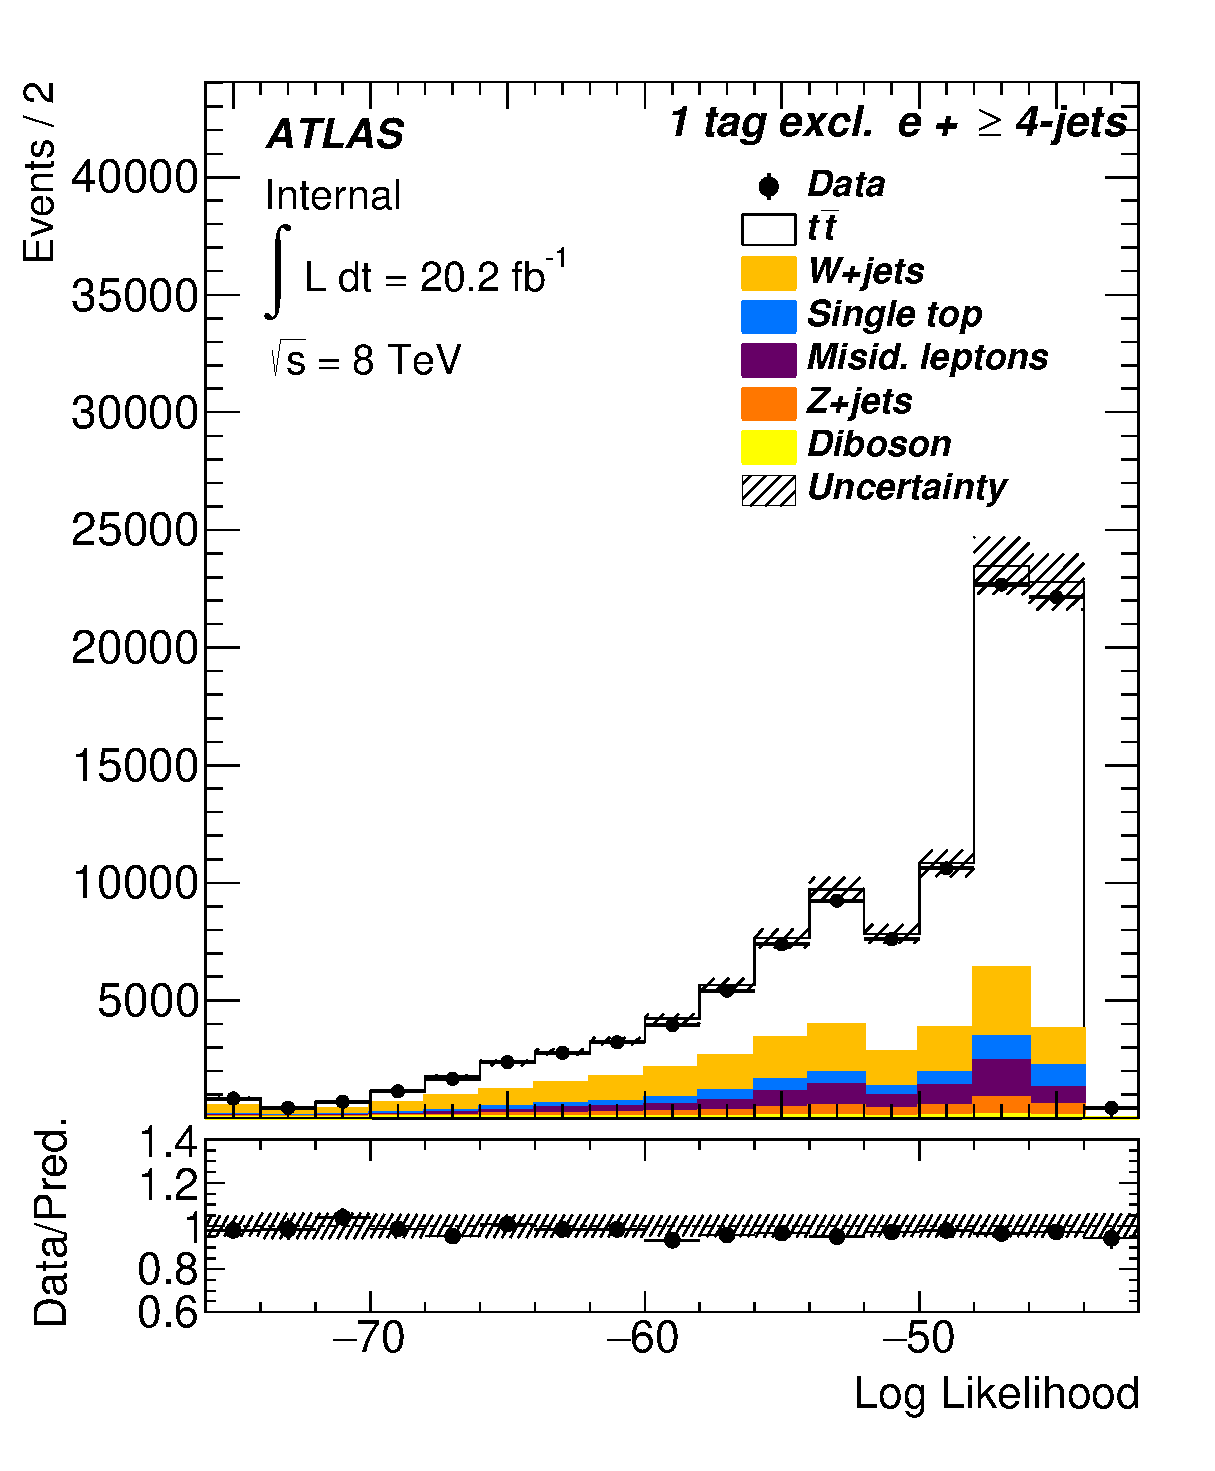
\includegraphics[height=65mm]{chapters/whel/figures/control_Plots2/bTag_1excl_NoLHCut/LogLikelihood_el}
        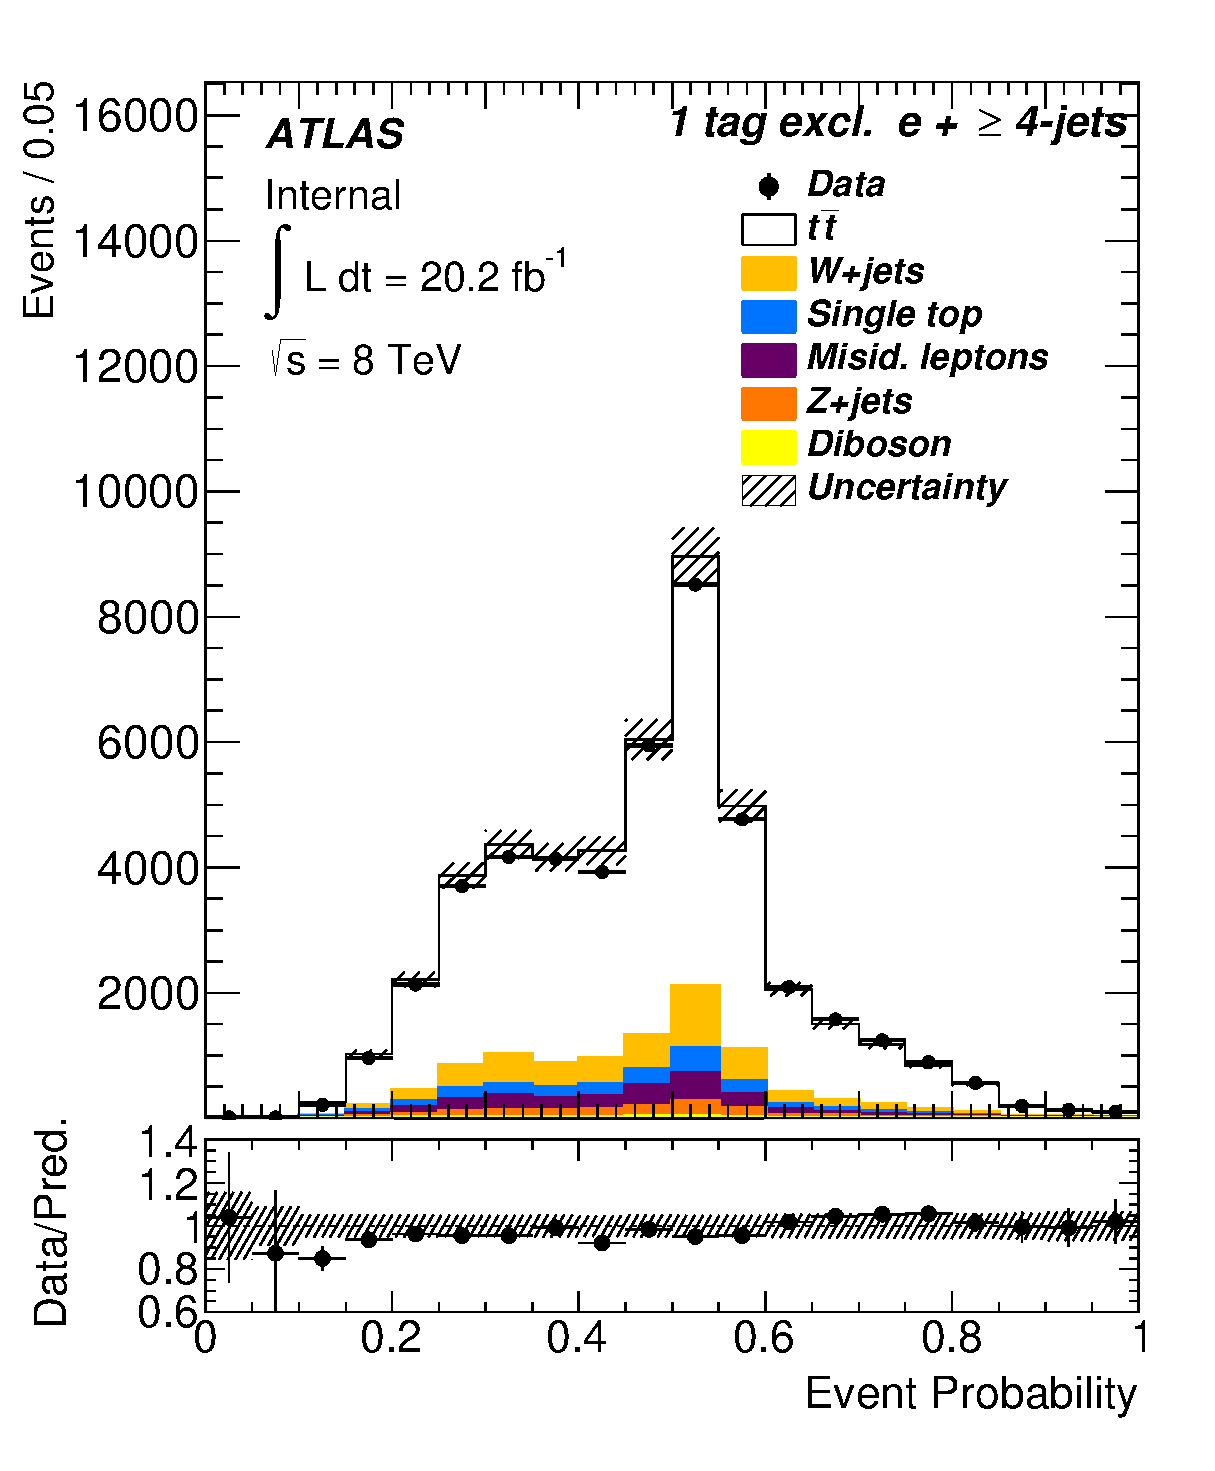
\includegraphics[height=65mm]{chapters/whel/figures/control_Plots2/bTag_1excl/EventProbability_el}
	\caption{Control distributions in the 1 exclusive \bt tag, electron channel for selected top kinematics, the log likelihood, and the event probability distributions of the leading permutation (ranked by event probability). All plots except for the log likelihood are shown after the cut LH $> -48$. The shaded bands represent the Monte Carlo statistical uncertainties.}
	\label{fig:klfitter_control_plots_1}
	\end{center}    
	\end{figure}    
	
\begin{figure}[!h]
\begin{center}
		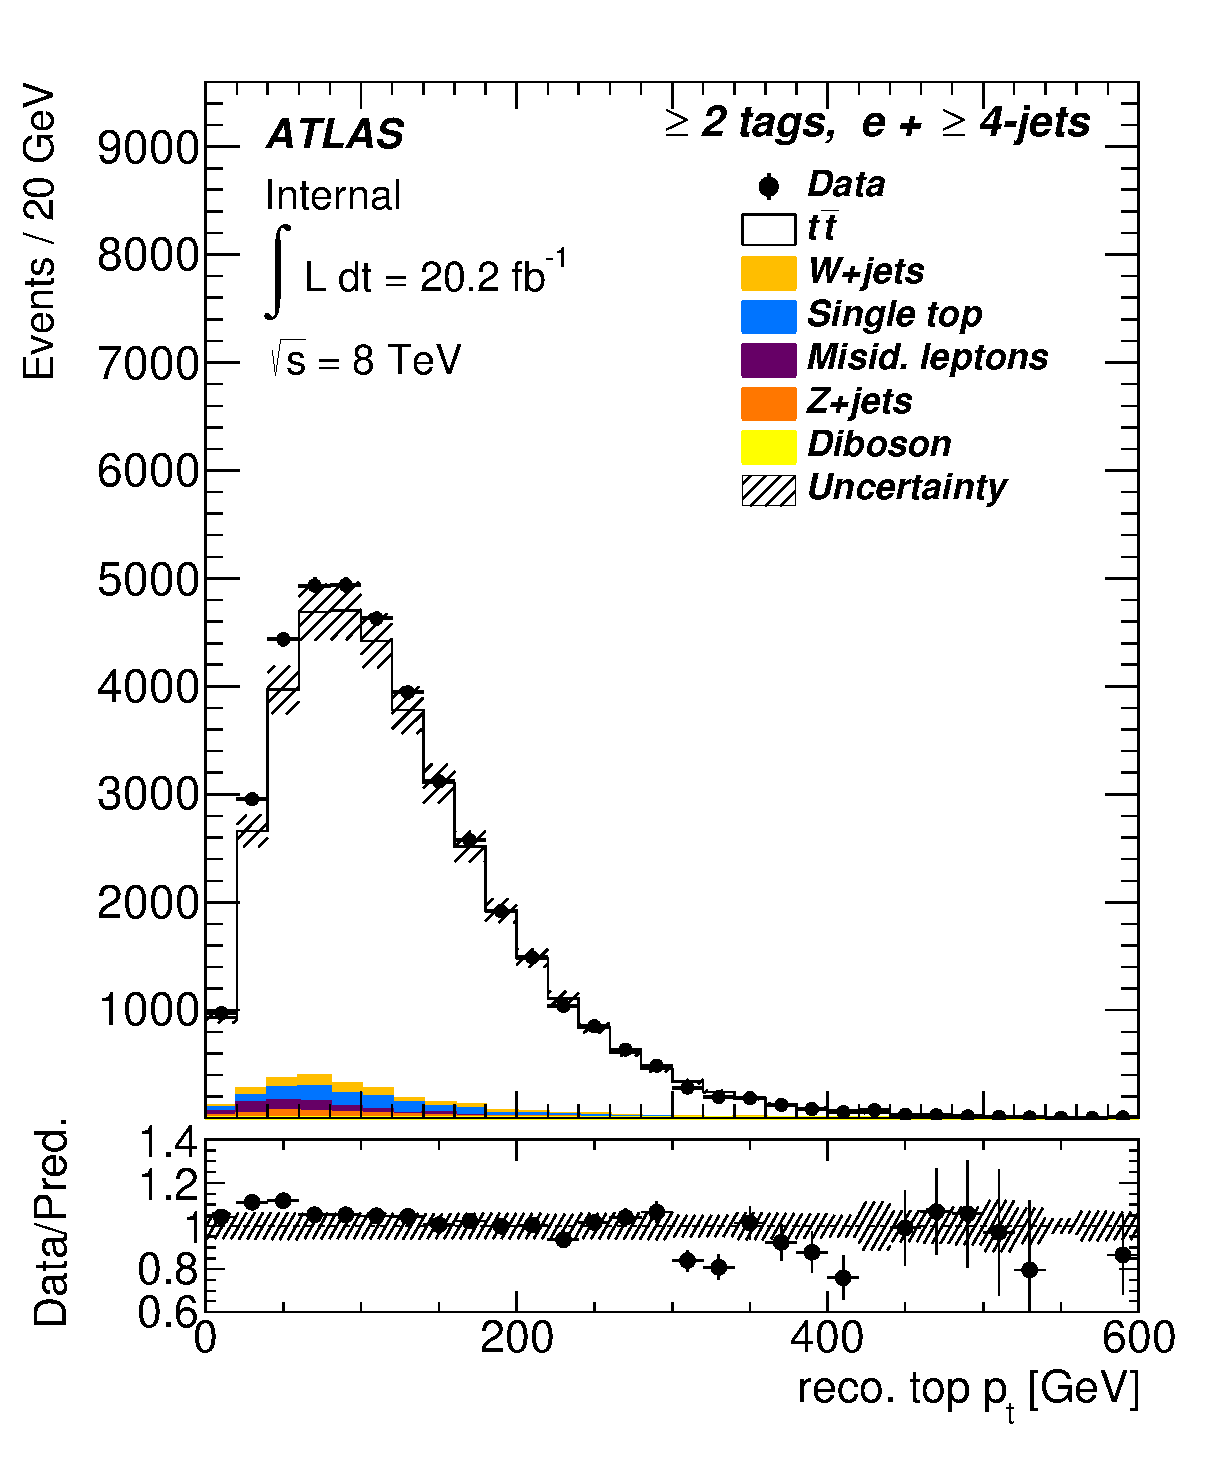
\includegraphics[height=65mm]{chapters/whel/figures/control_Plots2/bTag_2incl/reco_Top_pt_el}
		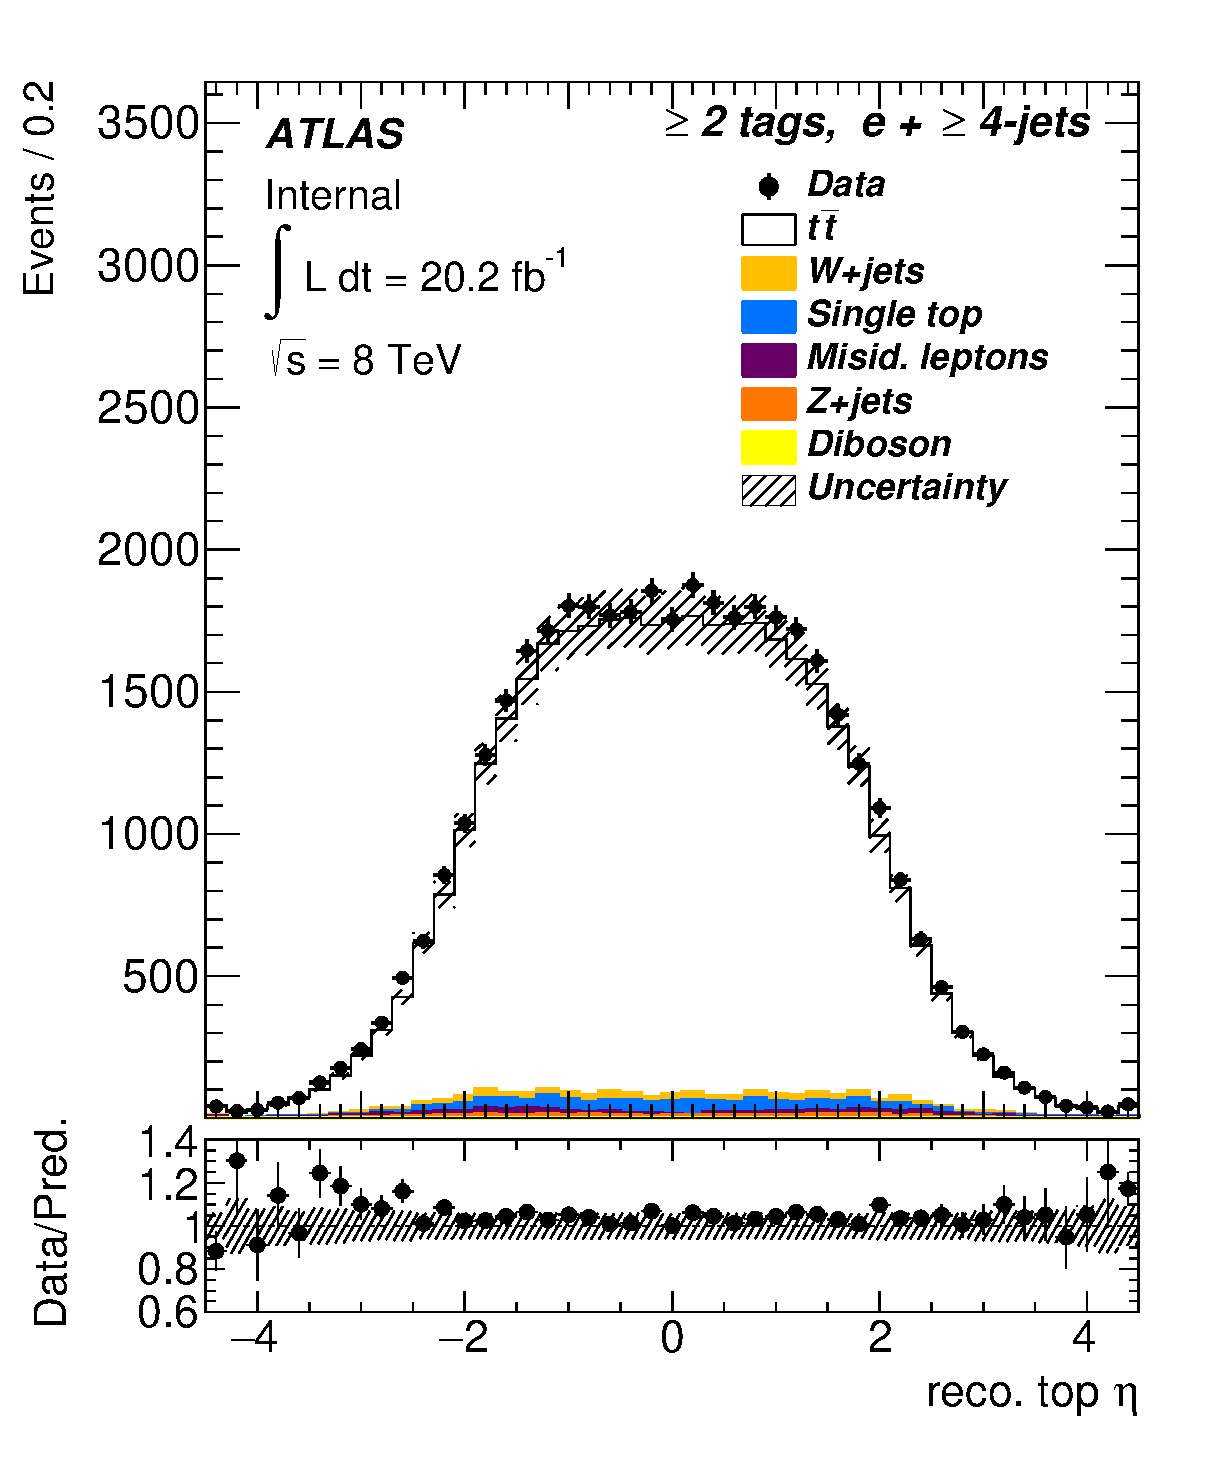
\includegraphics[height=65mm]{chapters/whel/figures/control_Plots2/bTag_2incl/reco_Top_eta_el}\\
		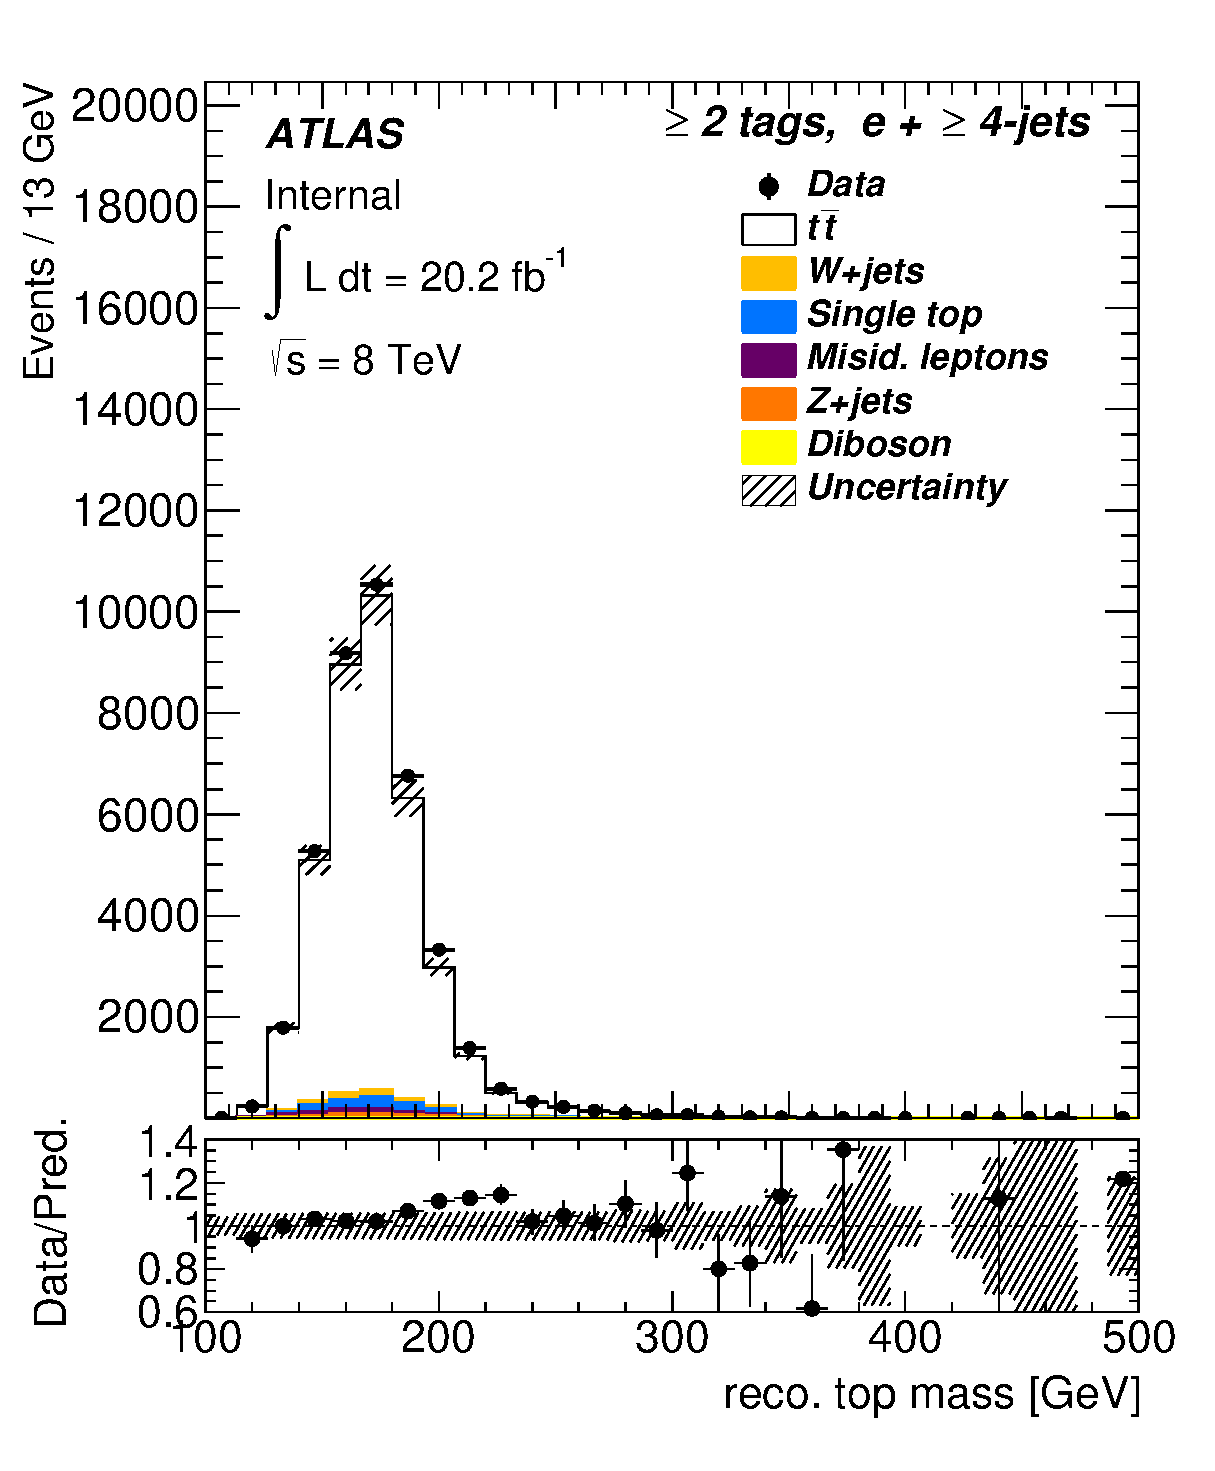
\includegraphics[height=65mm]{chapters/whel/figures/control_Plots2/bTag_2incl/reco_Top_m_el}
		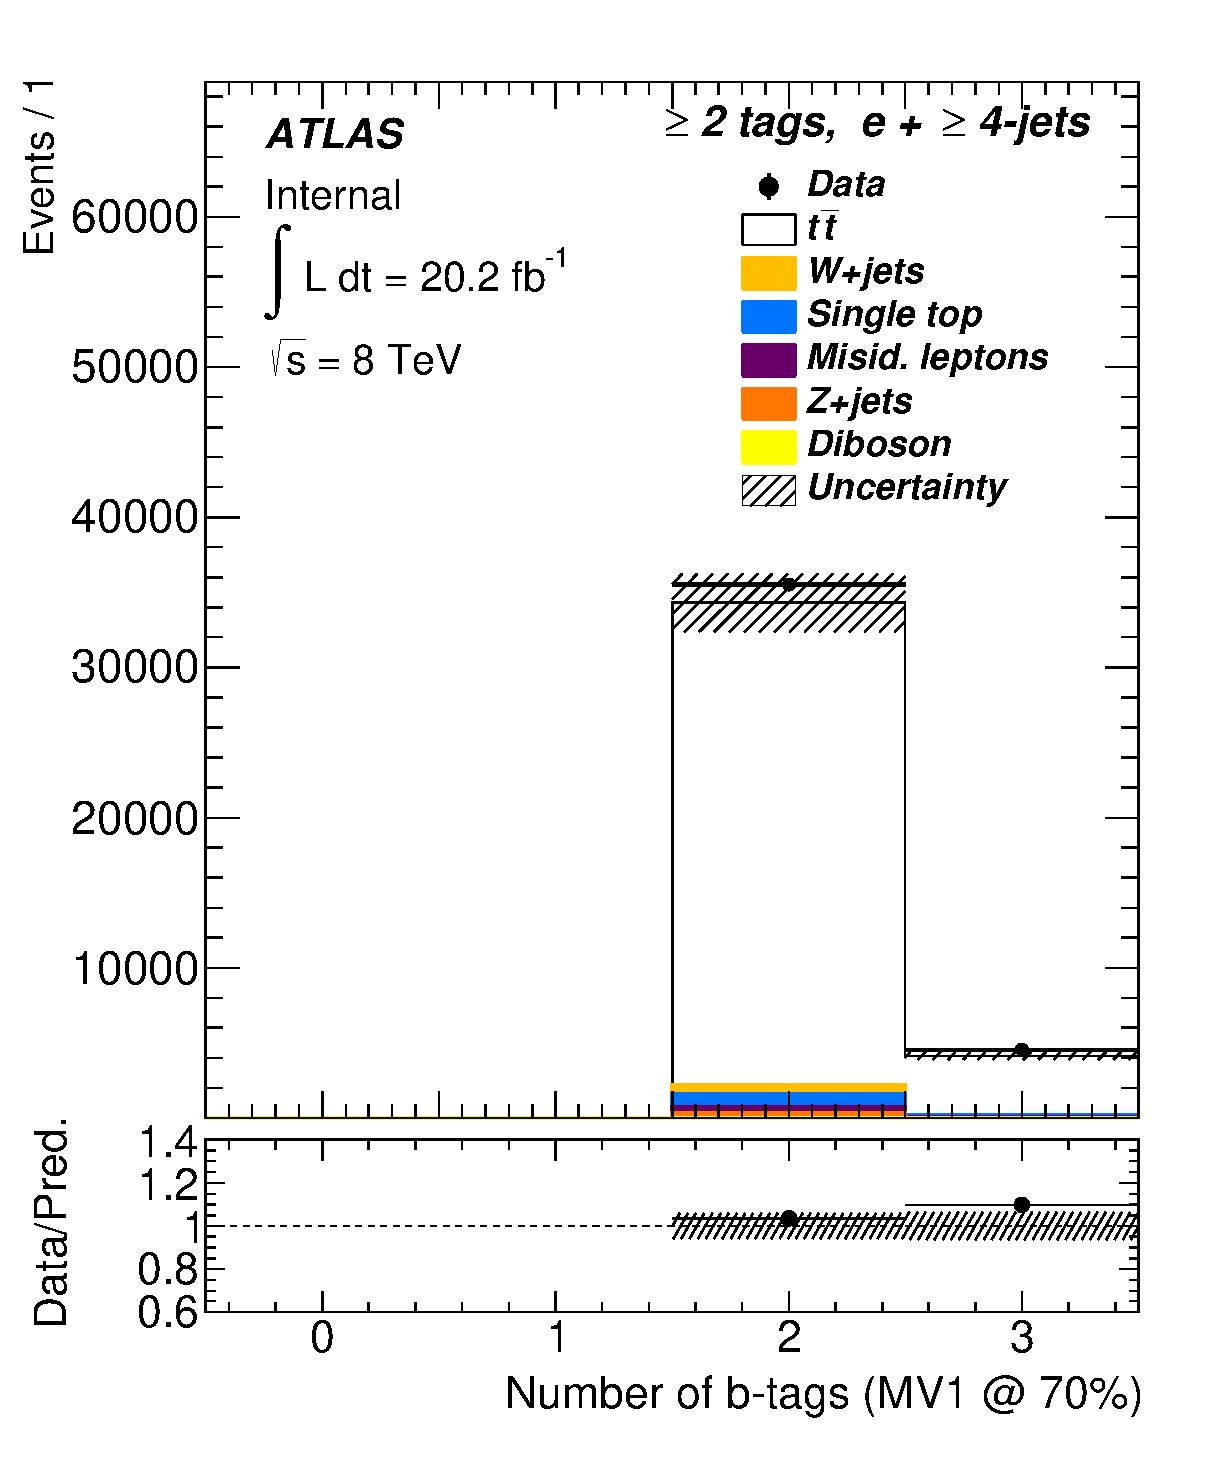
\includegraphics[height=65mm]{chapters/whel/figures/control_Plots2/bTag_2incl/NumberBtags_el}\\
		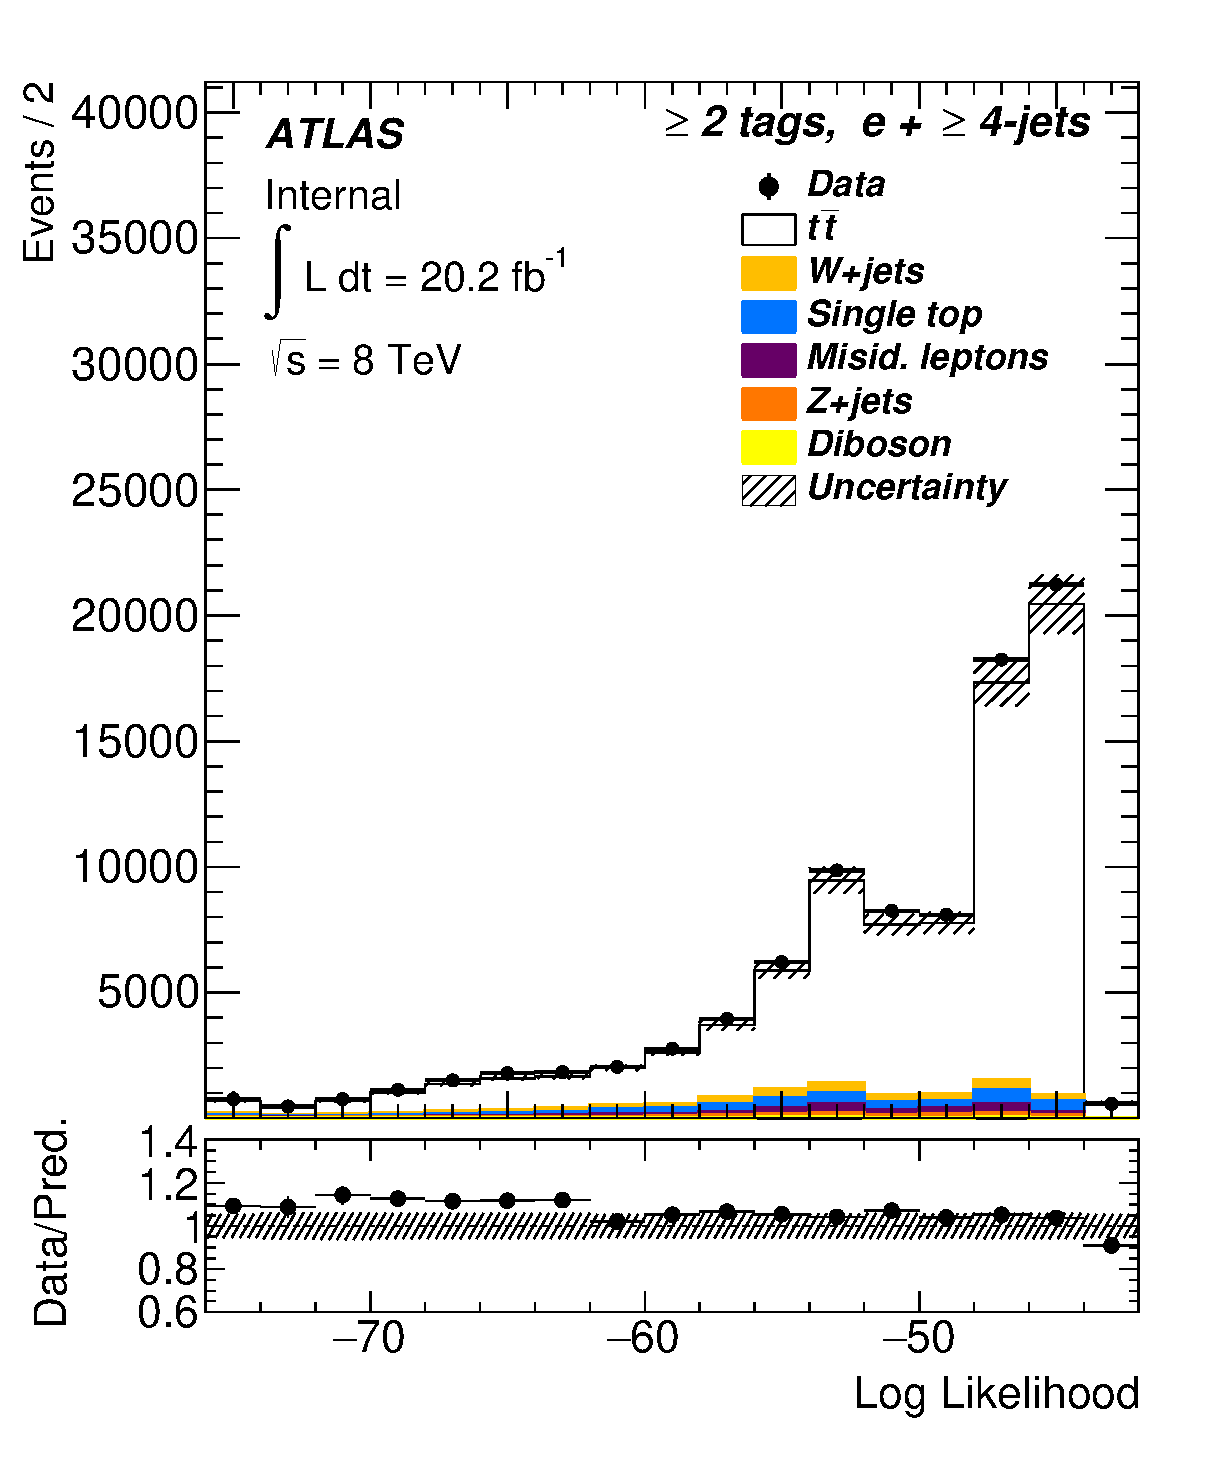
\includegraphics[height=65mm]{chapters/whel/figures/control_Plots2/bTag_2incl_NoLHCut/LogLikelihood_el}
        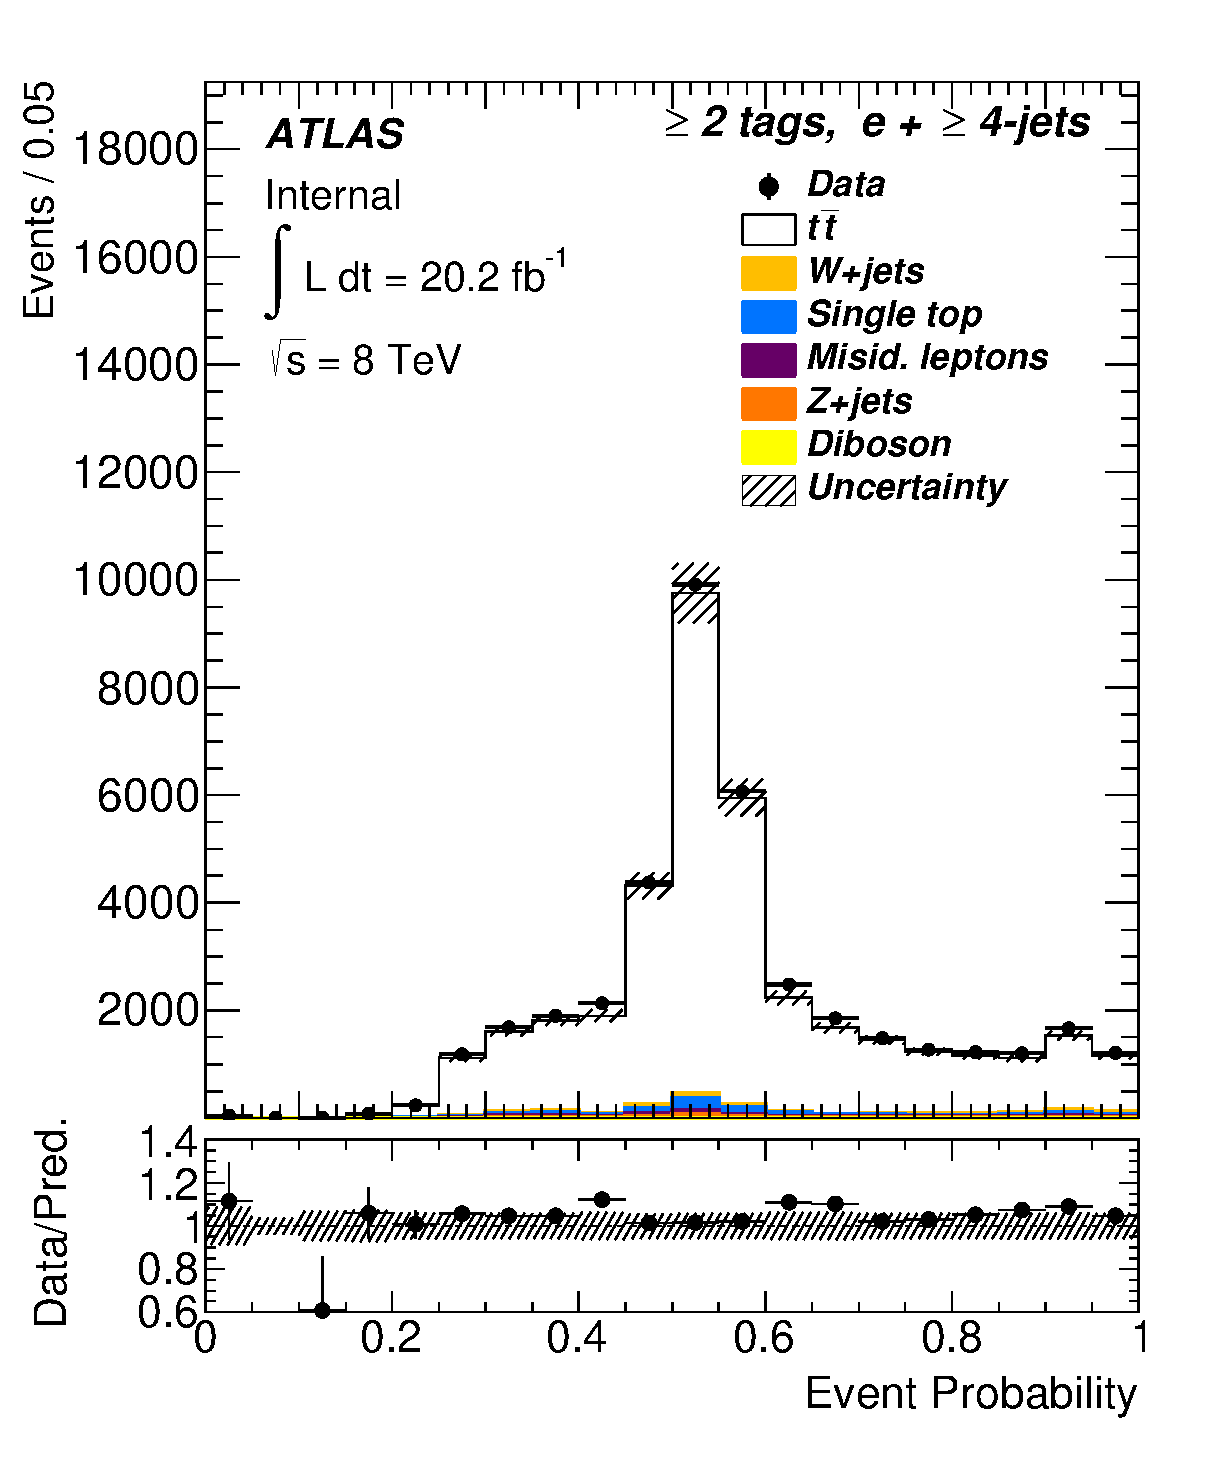
\includegraphics[height=65mm]{chapters/whel/figures/control_Plots2/bTag_2incl/EventProbability_el}
	\caption{Control distributions in the 2 inclusive \bt tag, electron channel for selected top kinematics, the log likelihood, and the event probability distributions of the leading permutation (ranked by event probability). All plots except for the log likelihood are shown after the cut LH $> -48$. The shaded bands represent the Monte Carlo statistical uncertainties.}
	\label{fig:klfitter_control_plots_2}
	\end{center}    
	\end{figure}
	
\begin{figure}[!h]
\begin{center}
		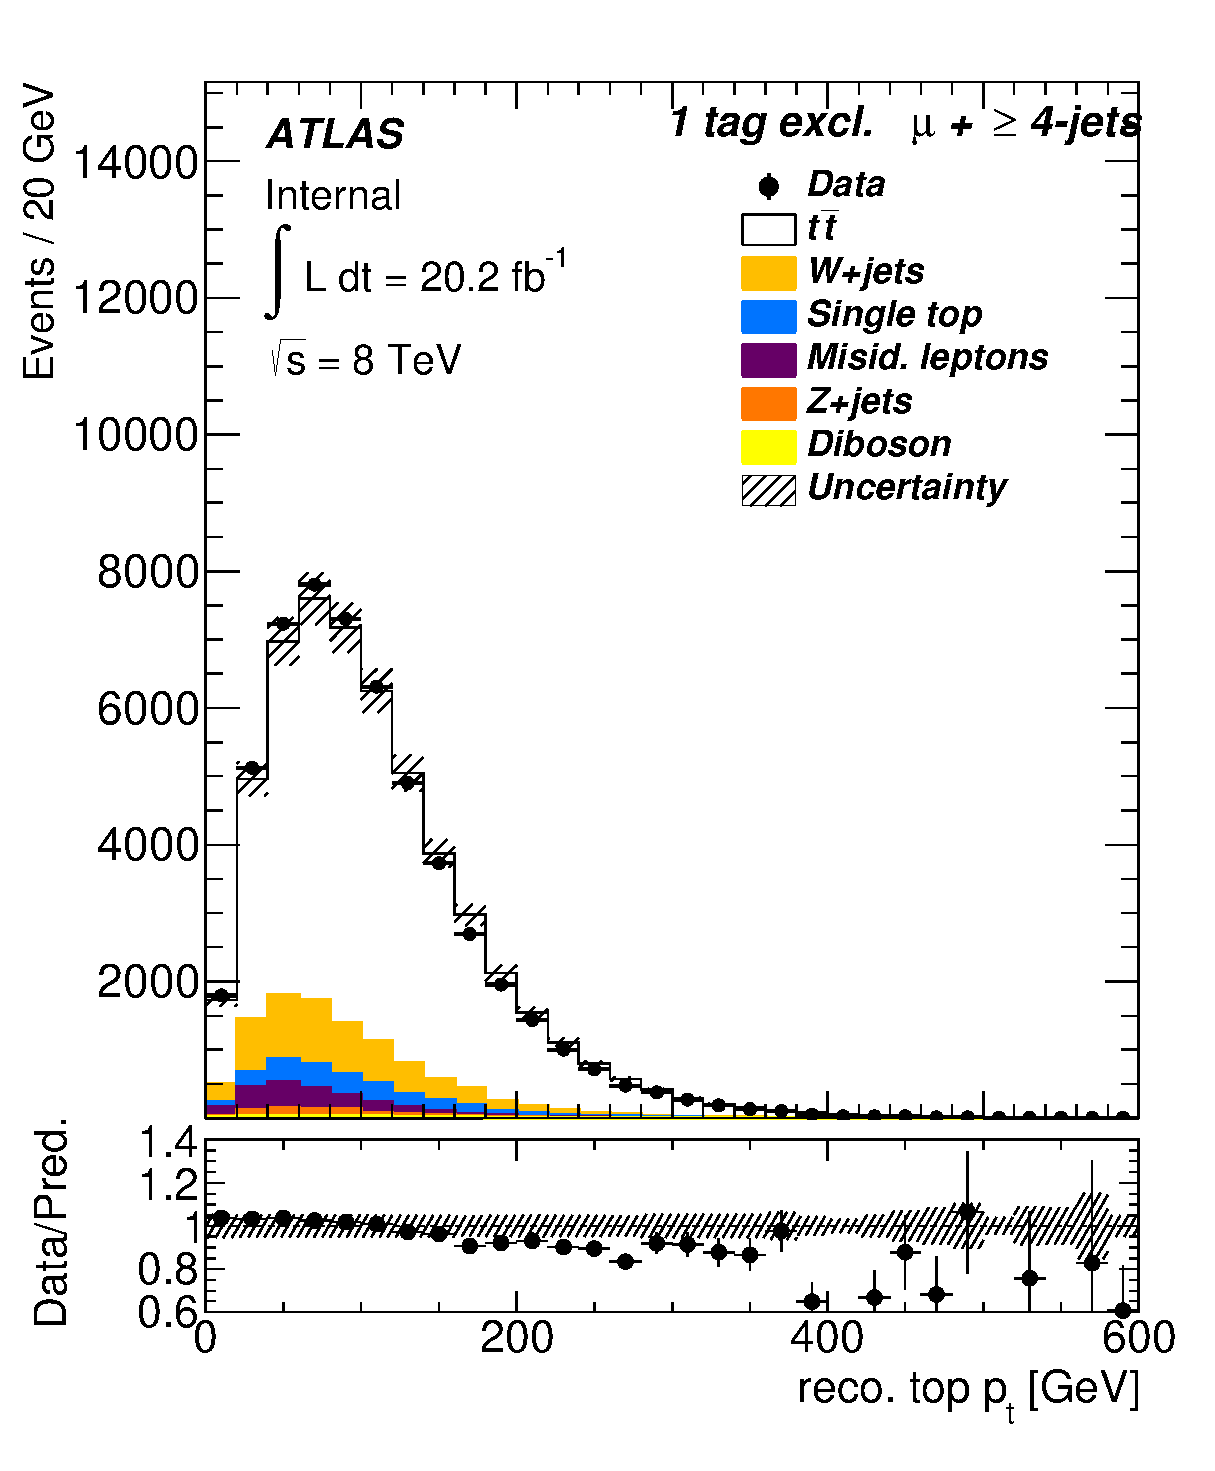
\includegraphics[height=65mm]{chapters/whel/figures/control_Plots2/bTag_1excl/reco_Top_pt_mu}
		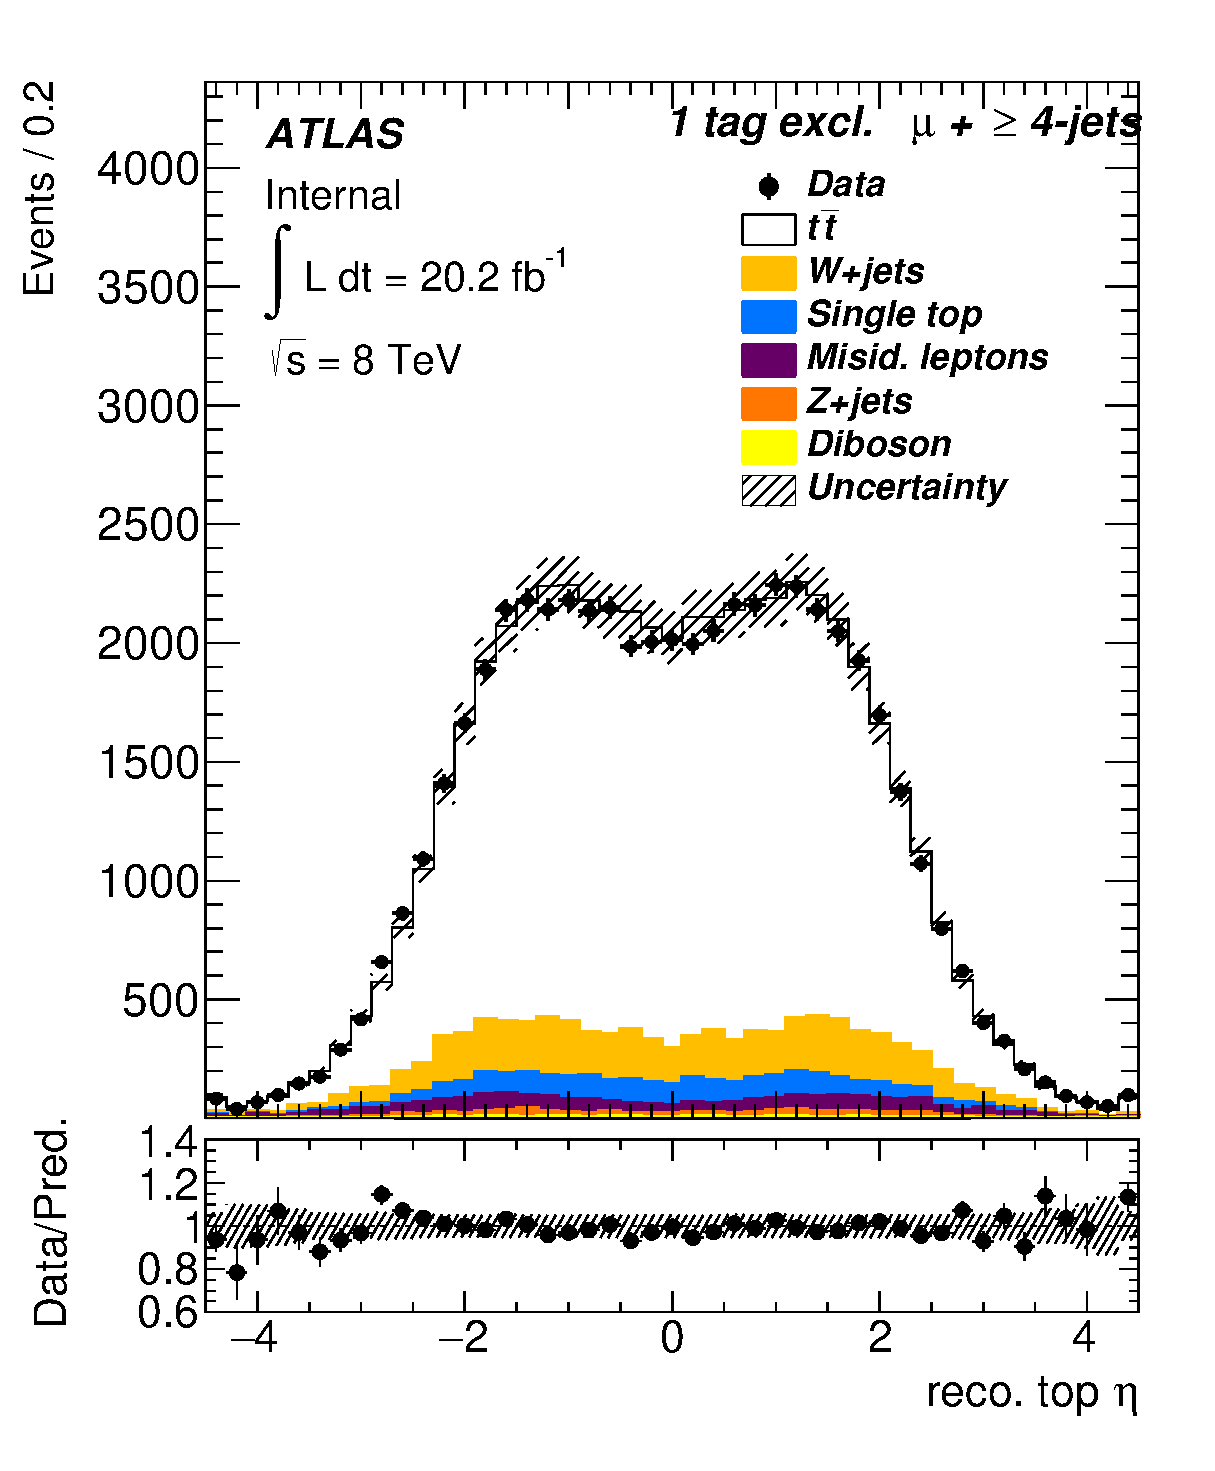
\includegraphics[height=65mm]{chapters/whel/figures/control_Plots2/bTag_1excl/reco_Top_eta_mu}\\
		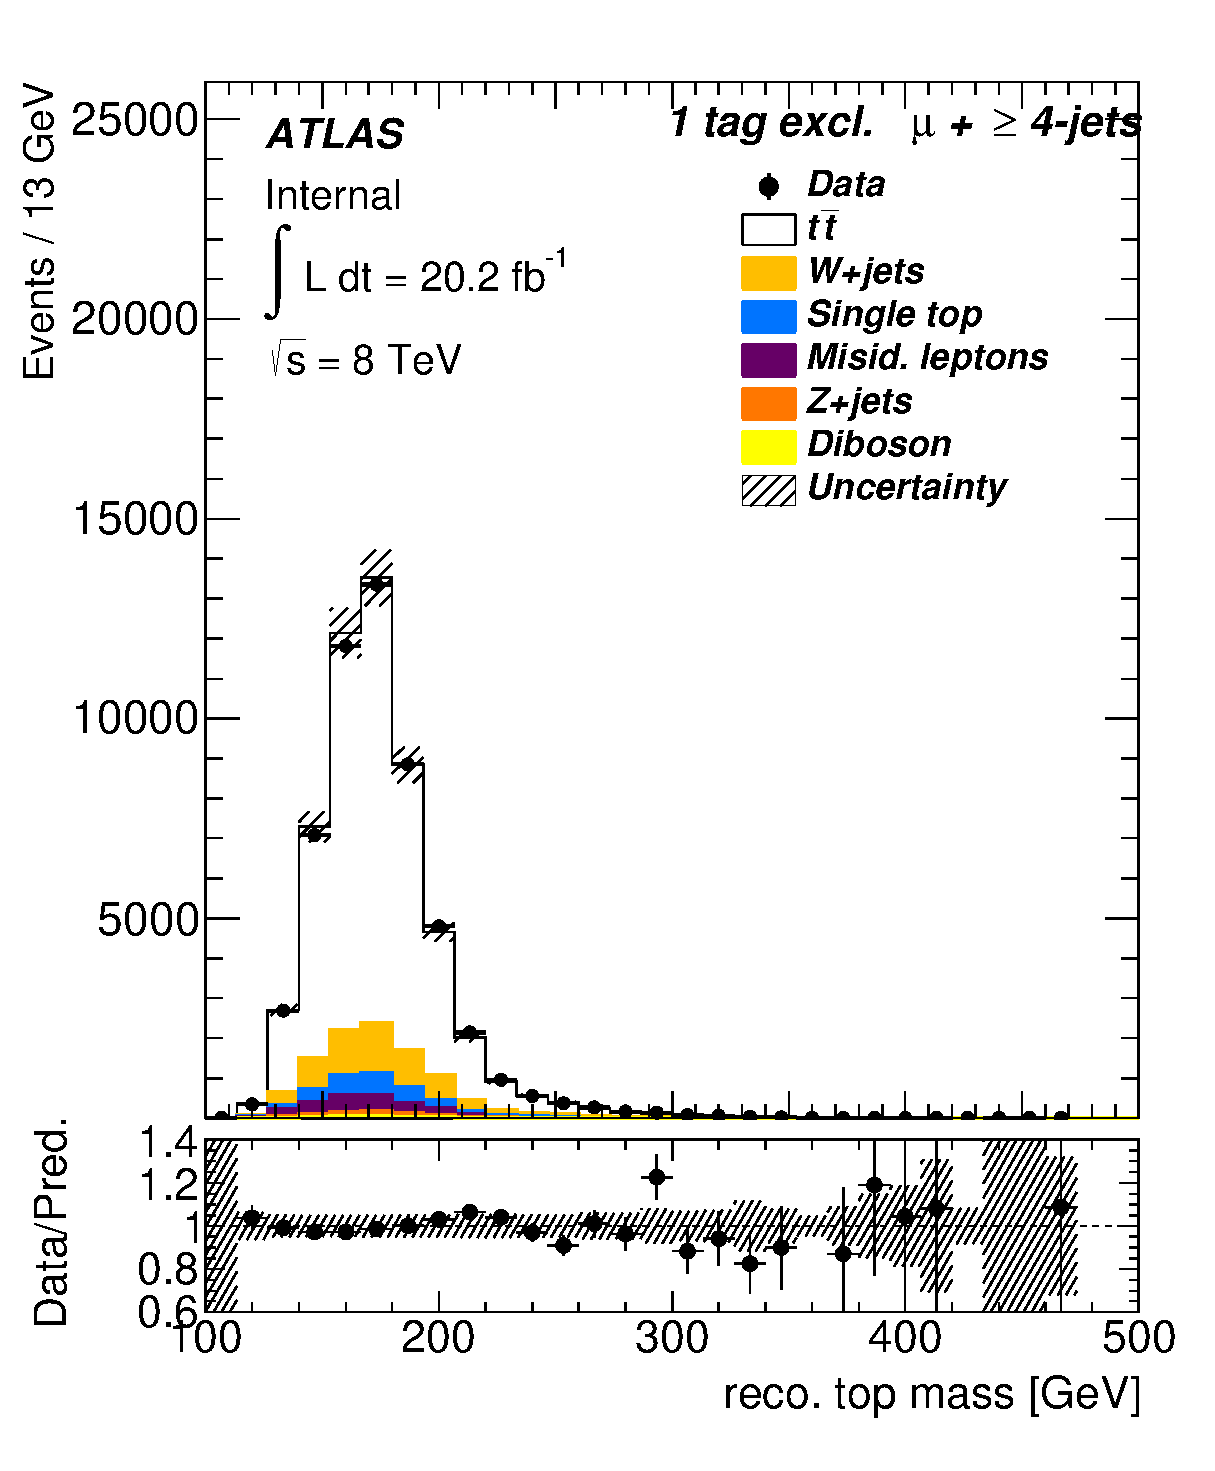
\includegraphics[height=65mm]{chapters/whel/figures/control_Plots2/bTag_1excl/reco_Top_m_mu}
		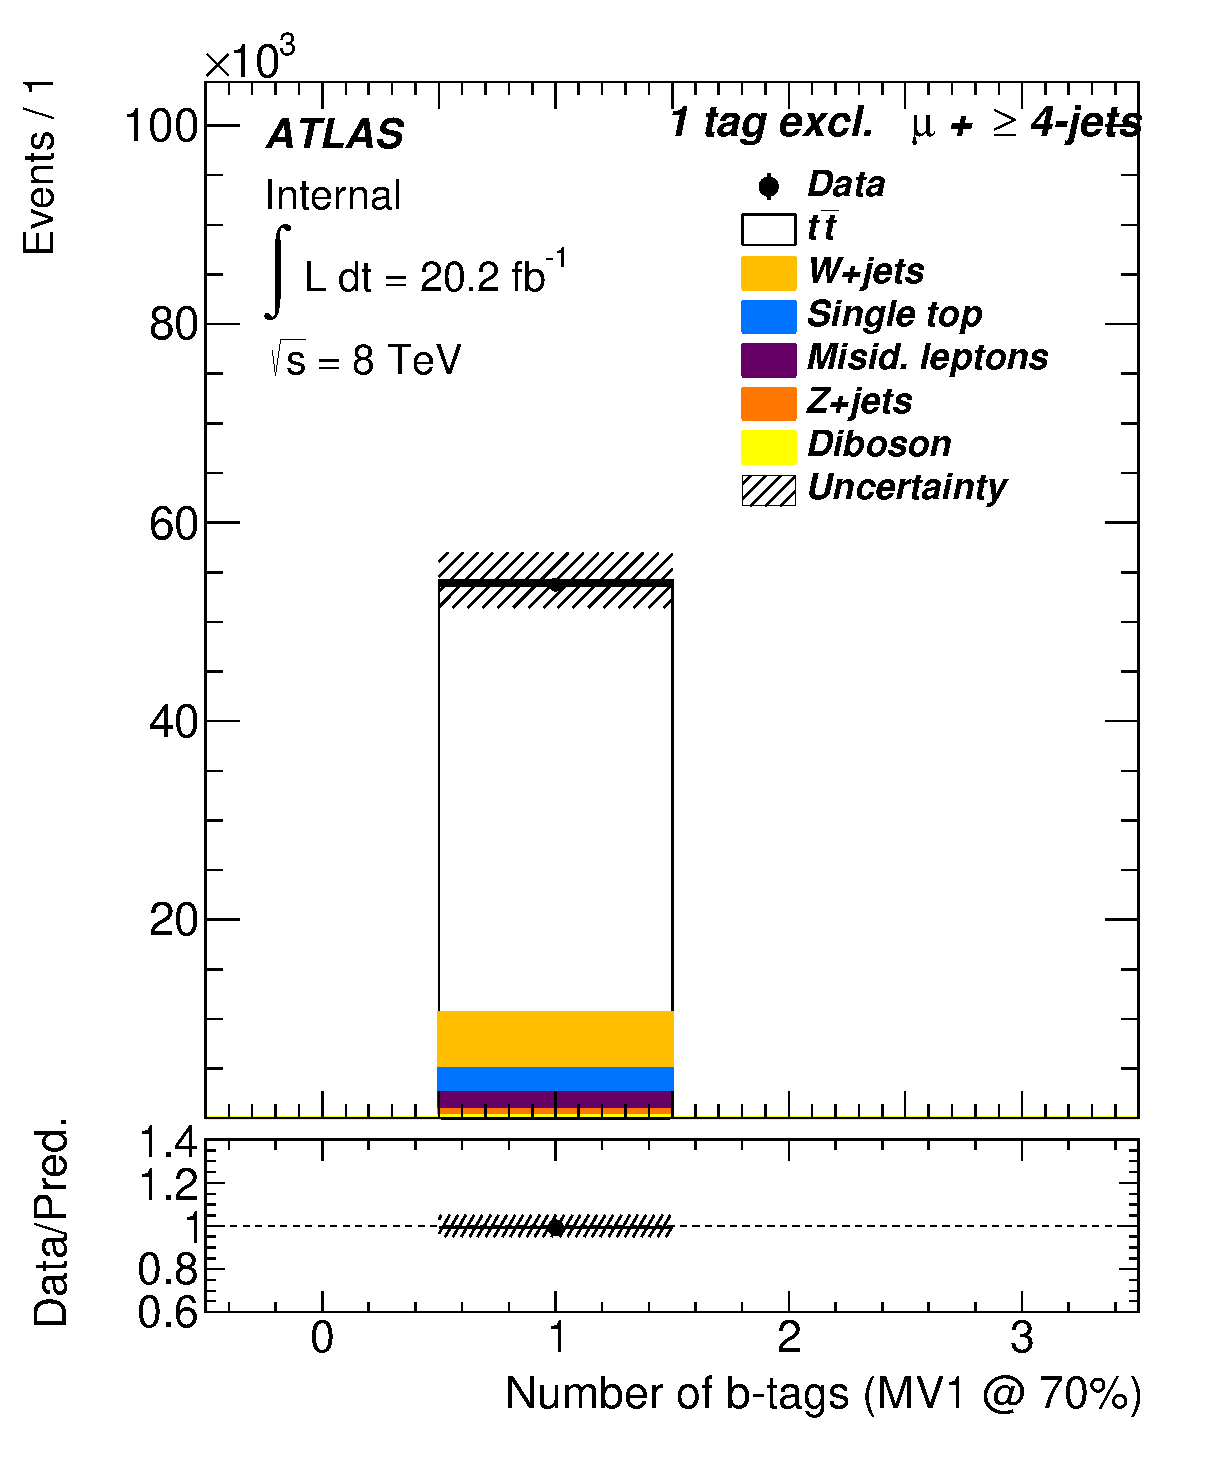
\includegraphics[height=65mm]{chapters/whel/figures/control_Plots2/bTag_1excl/NumberBtags_mu}\\
		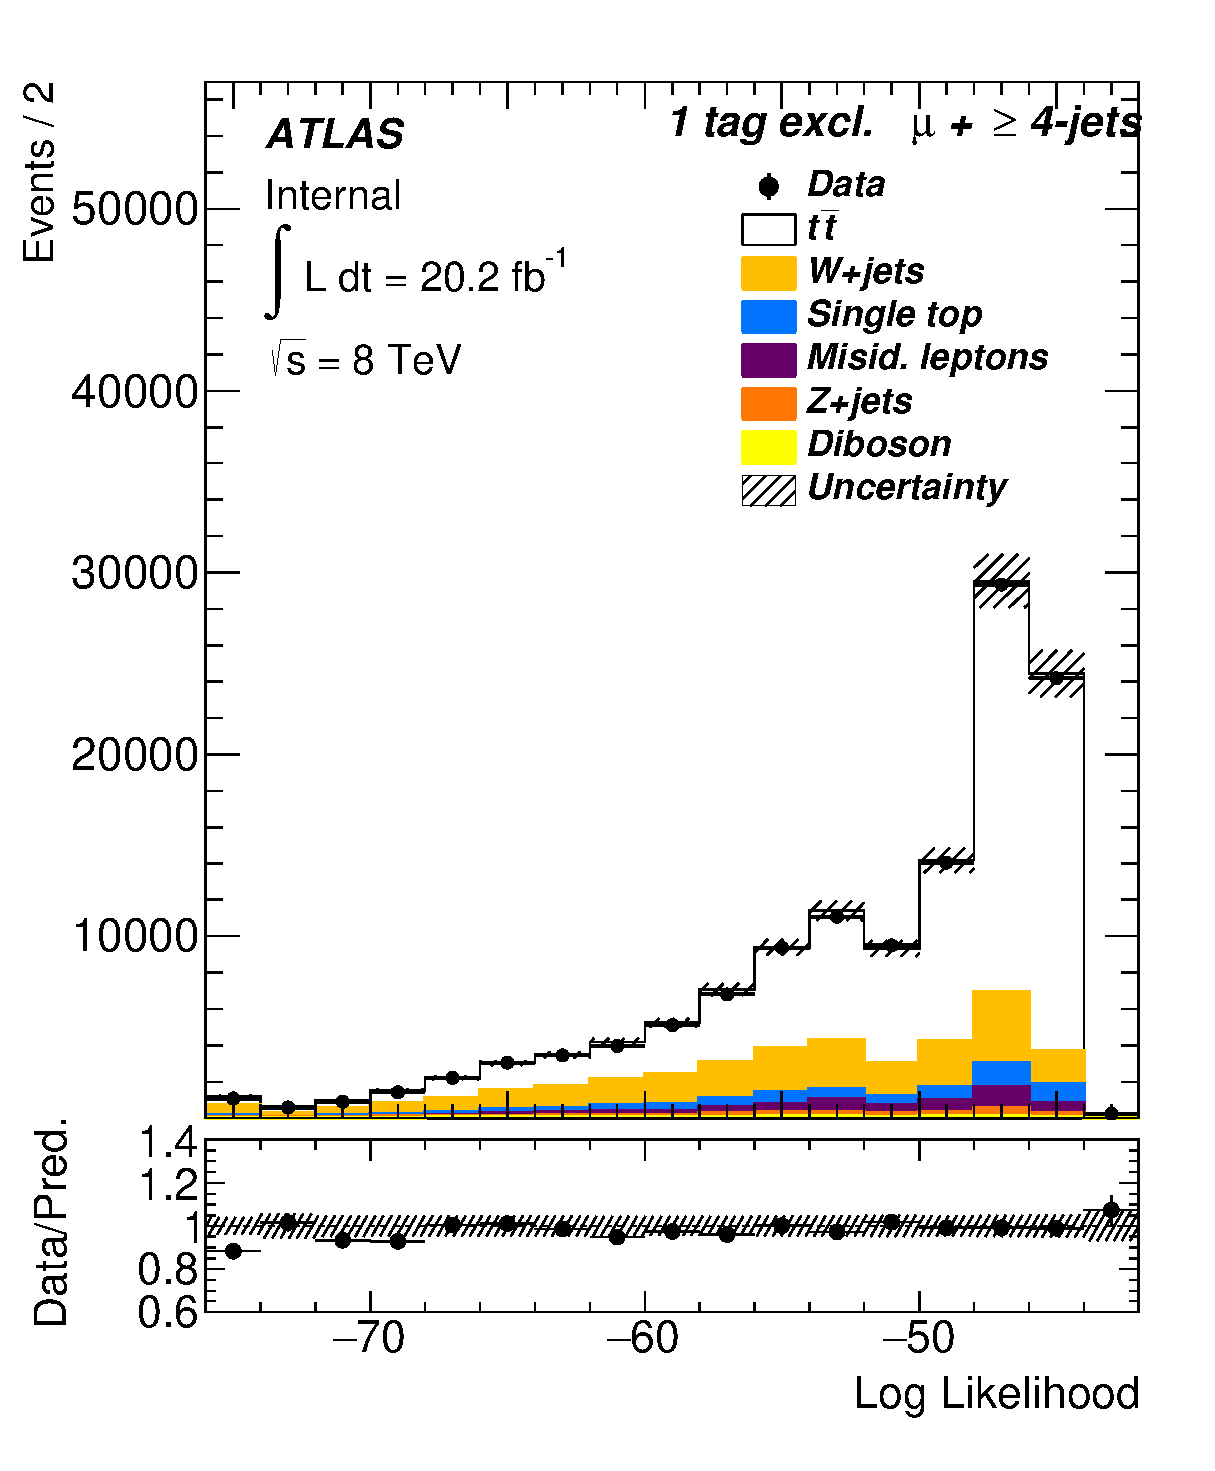
\includegraphics[height=65mm]{chapters/whel/figures/control_Plots2/bTag_1excl_NoLHCut/LogLikelihood_mu}
        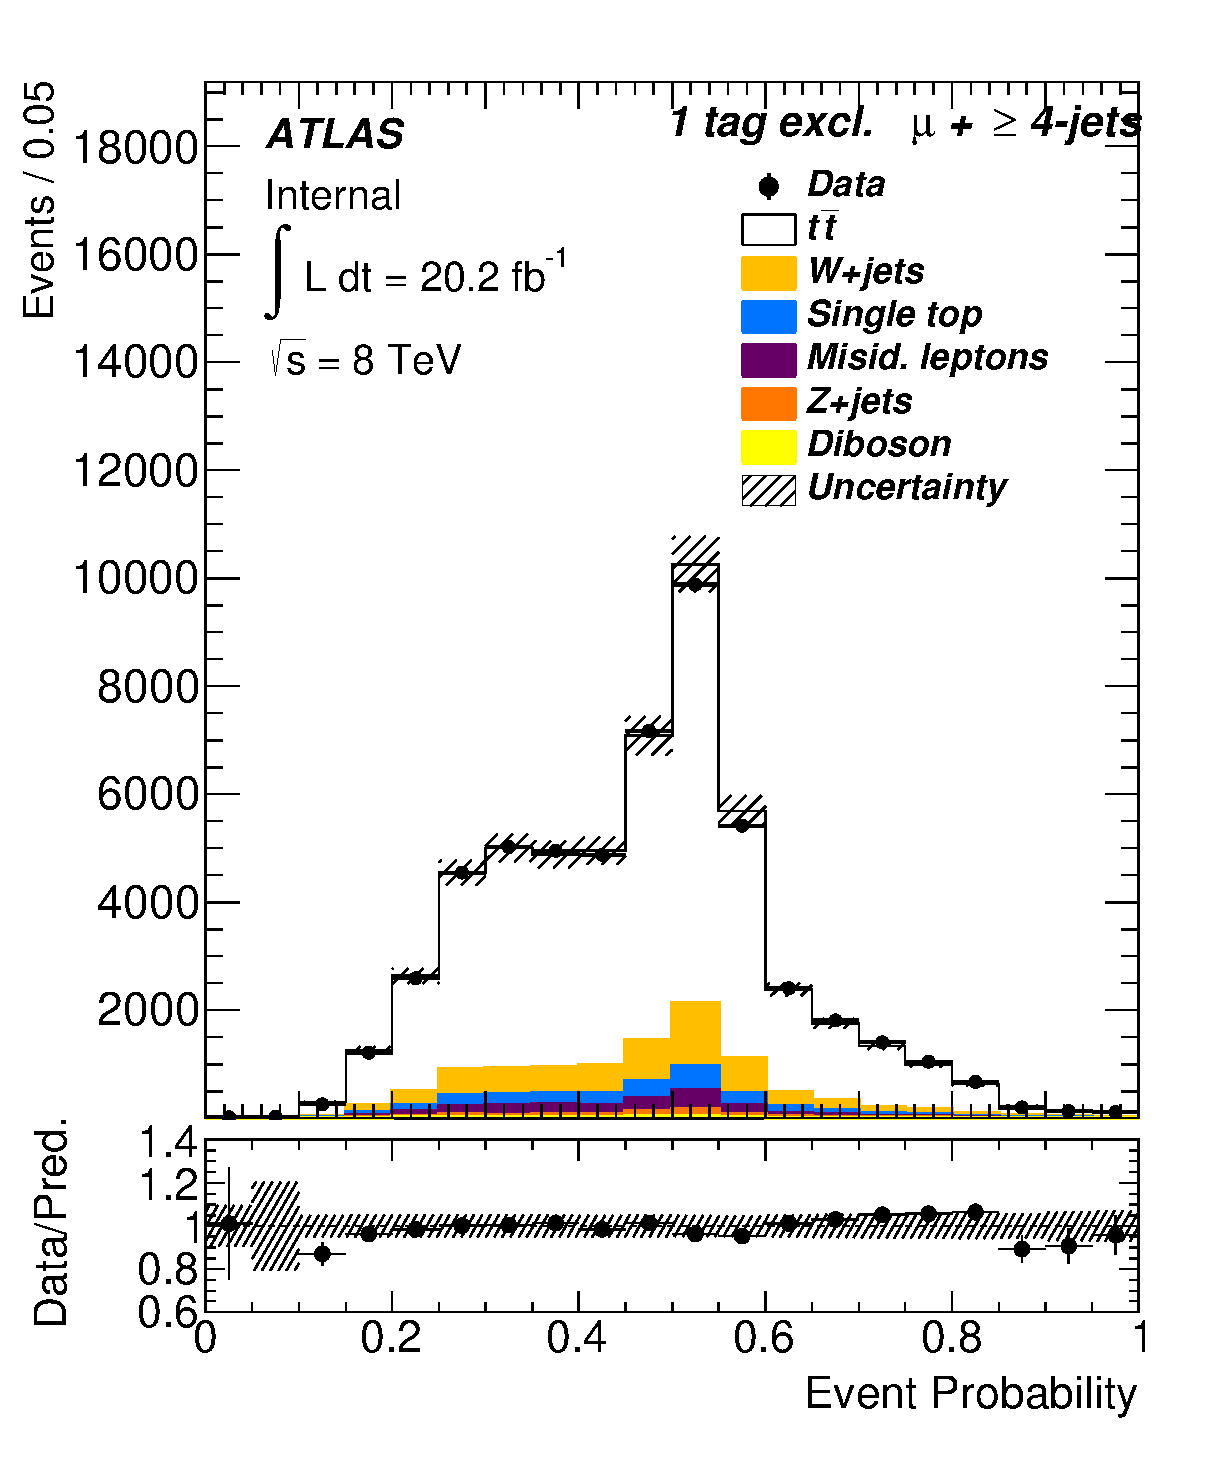
\includegraphics[height=65mm]{chapters/whel/figures/control_Plots2/bTag_1excl/EventProbability_mu}
	\caption{Control distributions in the 1 exclusive \bt tag, muon channel for selected top kinematics, the log likelihood, and the event probability distributions of the leading permutation (ranked by event probability). All plots except for the log likelihood are shown after the cut LH $> -48$. The shaded bands represent the Monte Carlo statistical uncertainties.}
	\label{fig:klfitter_control_plots_3}
	\end{center}    
	\end{figure}    
	
\begin{figure}[!h]
\begin{center}
		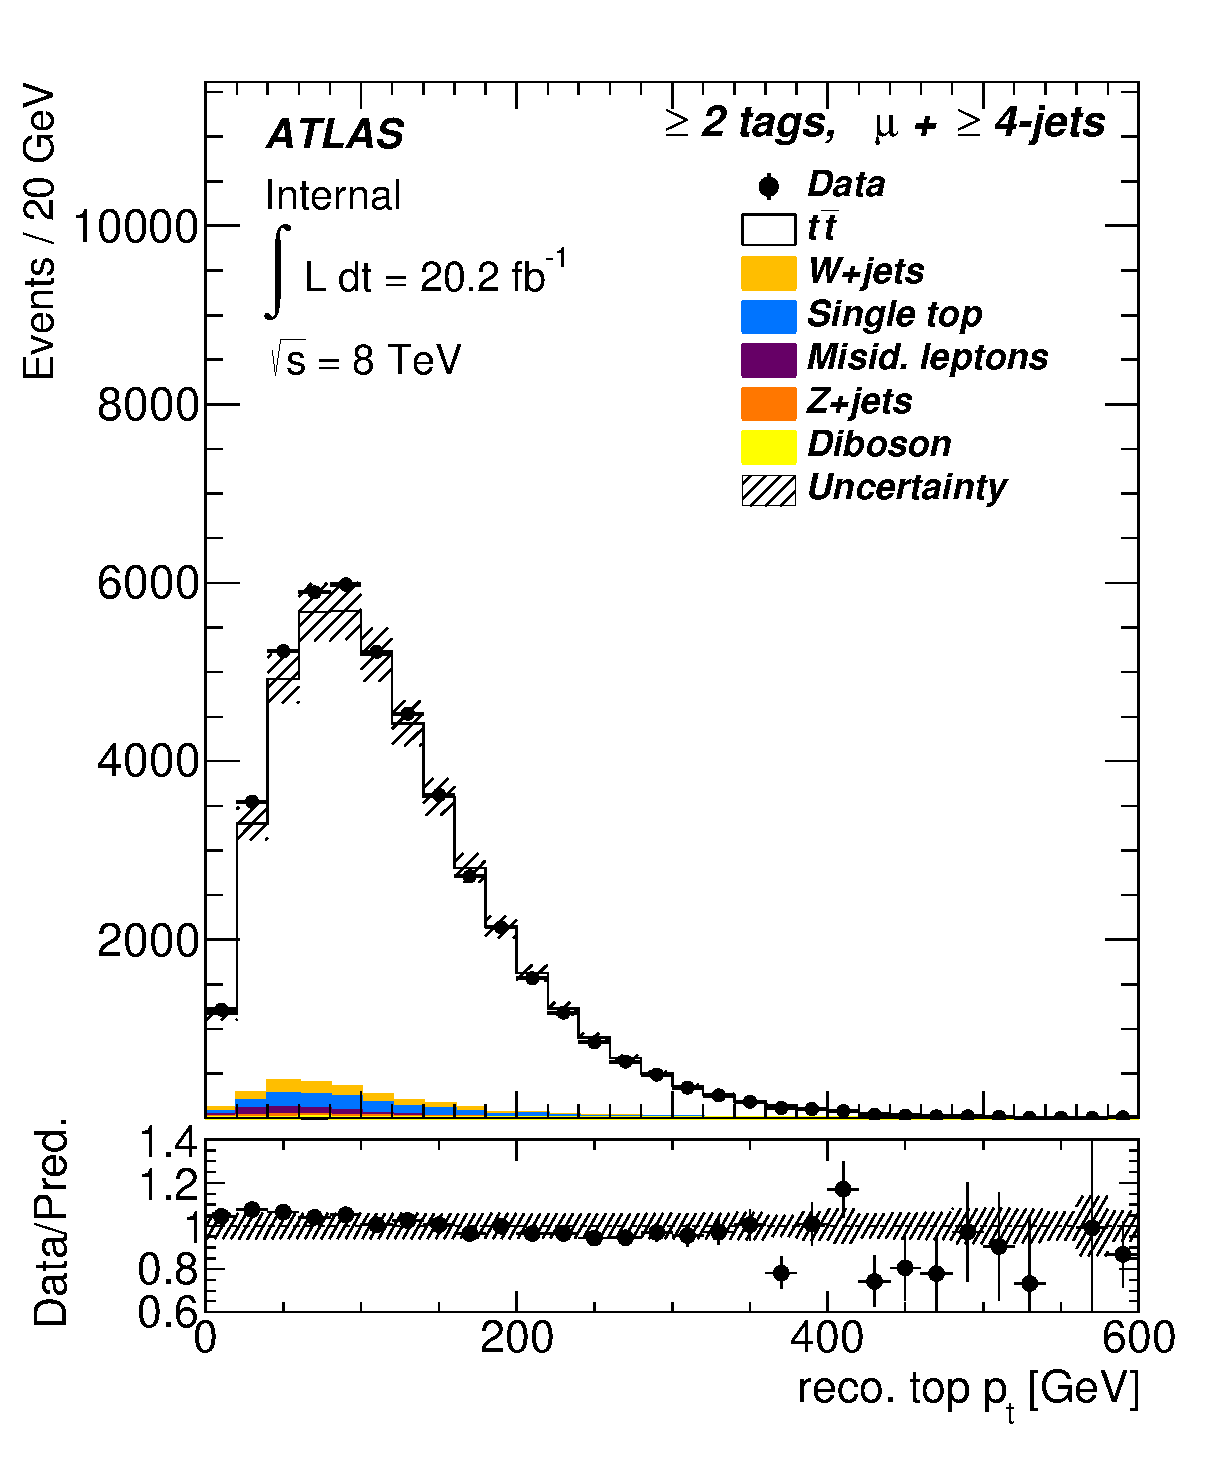
\includegraphics[height=65mm]{chapters/whel/figures/control_Plots2/bTag_2incl/reco_Top_pt_mu}
		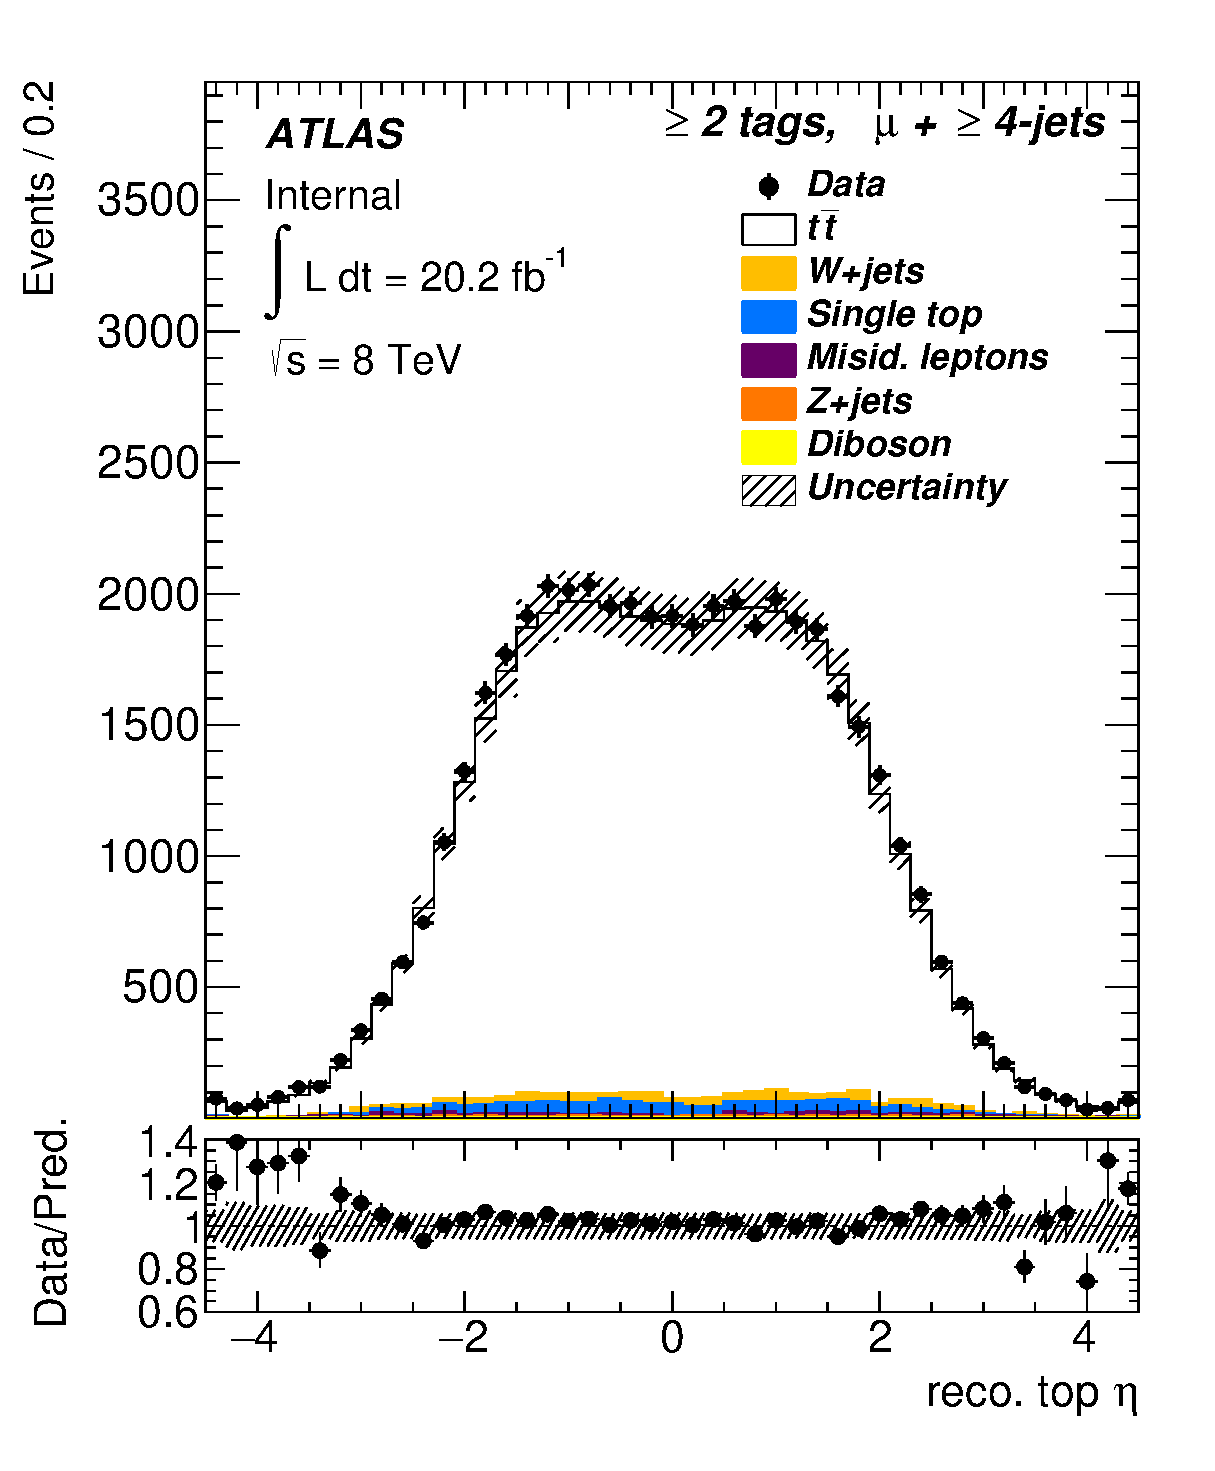
\includegraphics[height=65mm]{chapters/whel/figures/control_Plots2/bTag_2incl/reco_Top_eta_mu}\\
		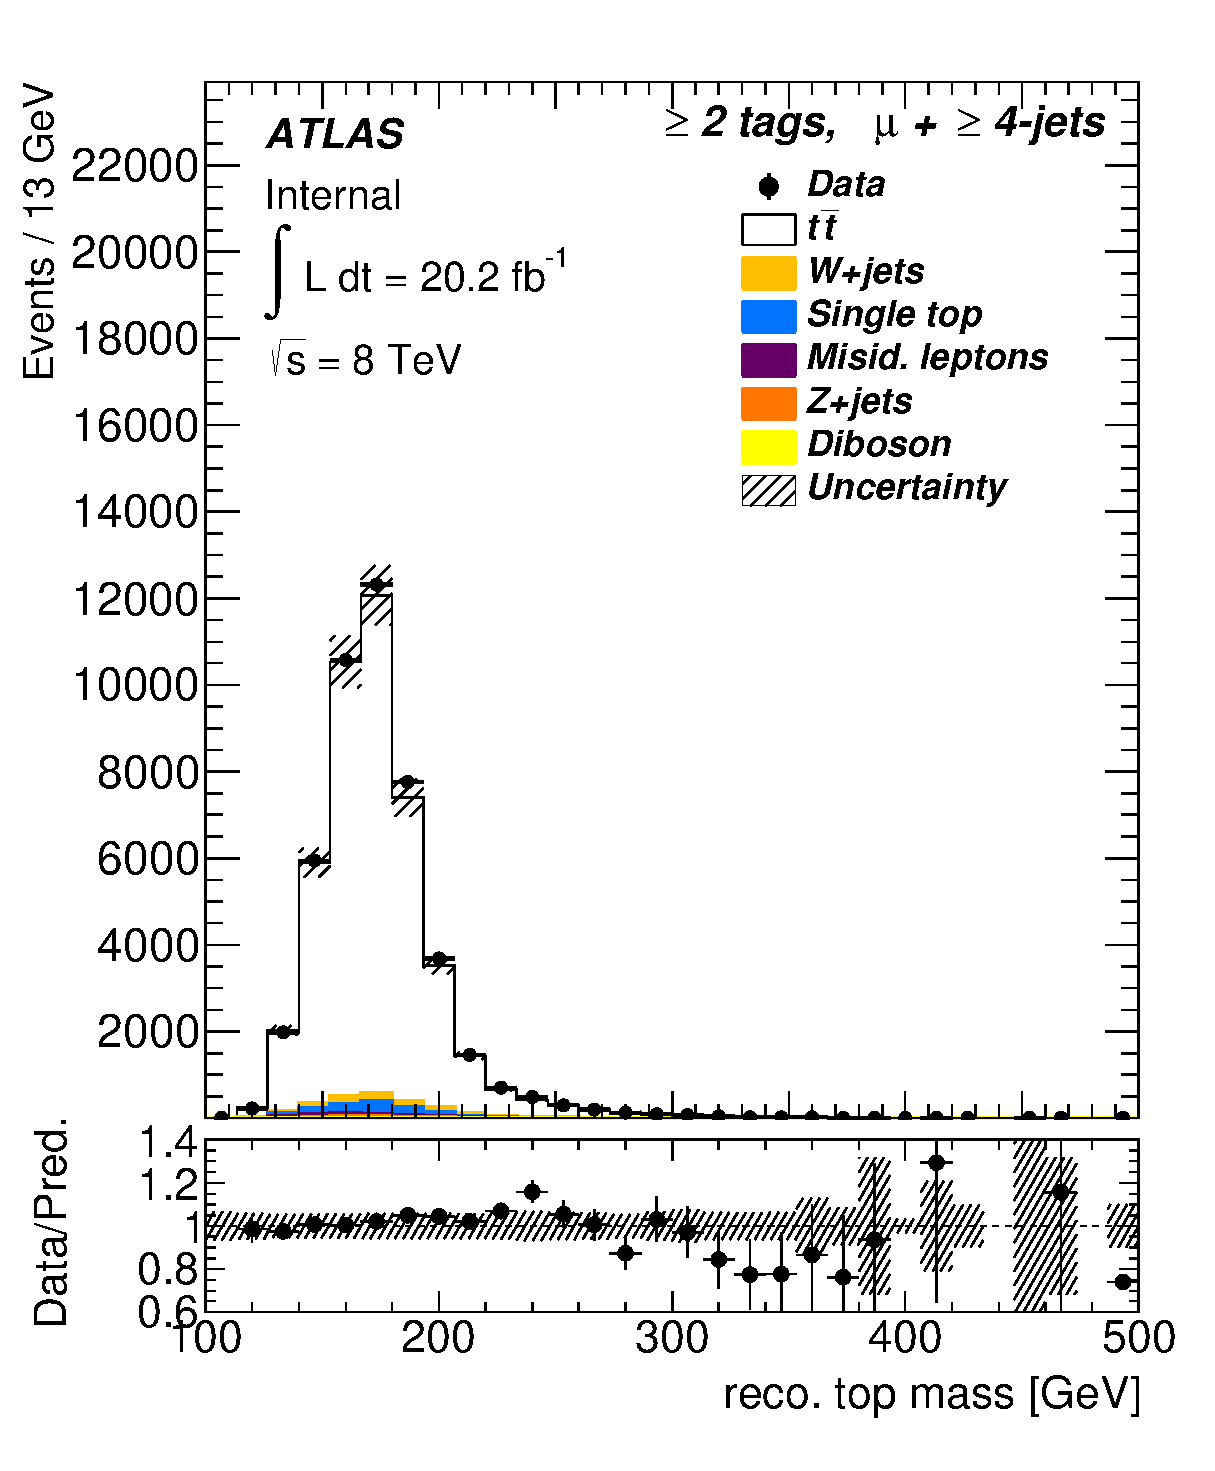
\includegraphics[height=65mm]{chapters/whel/figures/control_Plots2/bTag_2incl/reco_Top_m_mu}
		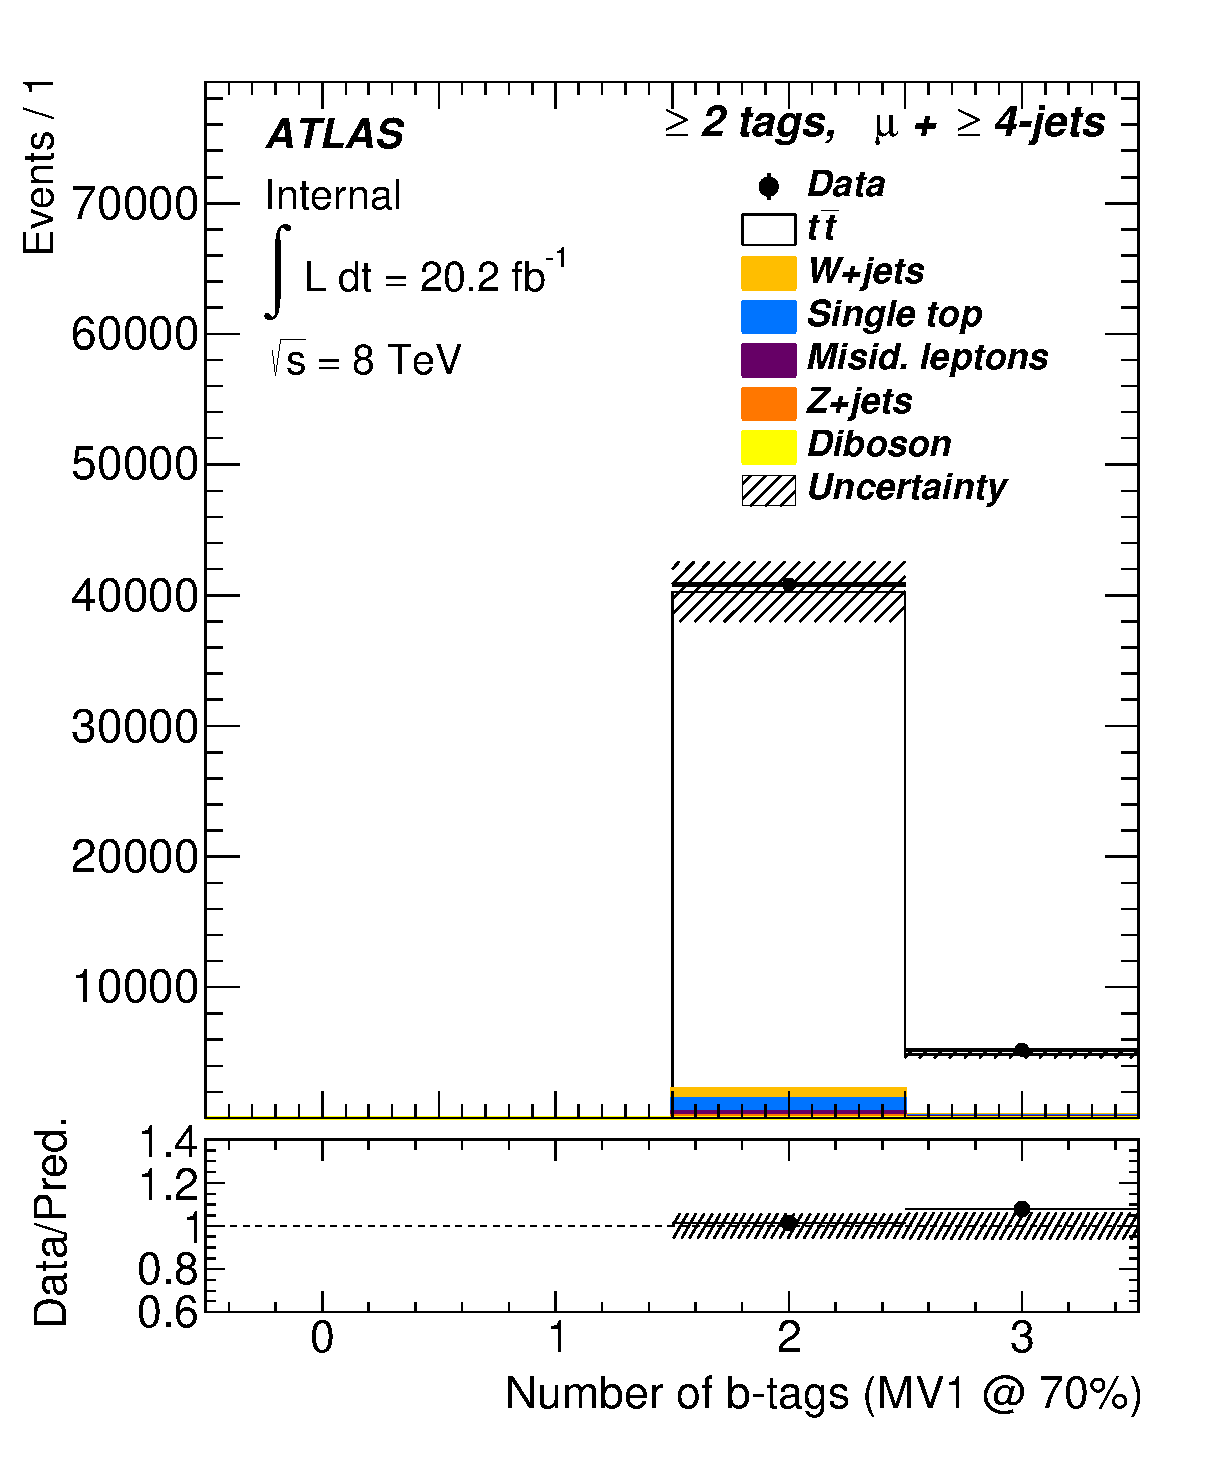
\includegraphics[height=65mm]{chapters/whel/figures/control_Plots2/bTag_2incl/NumberBtags_mu}\\
		\includegraphics[height=65mm]{chapters/whel/figures/control_Plots2/bTag_2incl_NoLHCut/LogLikelihood_mu}
        \includegraphics[height=65mm]{chapters/whel/figures/control_Plots2/bTag_2incl/EventProbability_mu}

	\caption{Control distributions in the 2 inclusive \bt tag, muon channel for selected top kinematics, the log likelihood, and the event probability distributions of the leading permutation (ranked by event probability). All plots except for the log likelihood are shown after the cut LH $> -48$. The shaded bands represent the Monte Carlo statistical uncertainties.}
	\label{fig:klfitter_control_plots_4}
	\end{center}    
	\end{figure}
%\clearpage
\subsection{Transfer Functions}
\label{sec:TF}
The transfer functions (TF) used in the kinematic fitter are derived for electrons, muons, light jets, \bt jets, and \met using the 8 TeV \ttbar MC sample described in Section \ref{sec:backgroundAndSignalModelling}. The difference between reconstructed energy and truth-level energy is fit using a double Gaussian functional form to determine the detector response for jets and electrons. A double Gaussian functional form was chosen in order to allow for the modeling of asymmetric tails in the detector response. The functional form of the transfer functions is given by
\begin{eqnarray}
W(\Delta E)=\frac{1}{\sqrt{2\pi}(p_2+p_3p_5)}\left[ e^{\frac{-(\Delta E-p_1)^2}{2p_2^2}}+p_3\cdot e^{\frac{-(\Delta E-p_4)^2}{2p_5^2}}\right]
\label{eq:TFeq}
\end{eqnarray}
where $\Delta E=\frac{E_{truth}-E_{reco}}{E_{truth}}$, and the parameters $p_i$ depend on the energy of the parton/lepton are parameterized depending on the parton/lepton type. As the best guess at leading order, a linear dependence is assumed. If another dependence is known by a physical motivation, the paramterization is adapted correspondingly. For example, in the case of jets and electrons, $p_2$ represents the calorimeter resolution and is hence parameterized as $\sim 1/\sqrt{E}$. If the linear assumption fails, it can also be replaced by heuristically determined parameterizations. In the case of electrons and jets, the parameterizations are 

\begin{eqnarray}
p_1=a_1+b_1\cdot E_{truth}\label{eq:TFp1}\\
p_2=a_2/\sqrt{E_{truth}}+b_2\label{eq:TFp2}\\
p_3=a_3+b_3\cdot E_{truth}\label{eq:TFp3}\\
p_4=a_4+b_4\cdot E_{truth}\label{eq:TFp4}\\
p_5=a_5+b_5\cdot E_{truth}\label{eq:TFp5}
\end{eqnarray}
The $a_i$'s and $b_i$'s are obtained from a global fit to each particle species and $\eta$ region. For muons, $E_{truth}$ is replaced with $p_{T}^{truth}$, and all $p_i$ are parameterized linearly, i.e. Equation~\ref{eq:TFp2} becomes $p_2=a_2+b_2\cdot E_{truth}$. 

Only reconstructed objects that are bi-uniquely (one and only one matching for both objects) matched to partons from the hard decay are used to derive the transfer functions. An object is considered matched if the $\Delta R$ between the reconstructed and truth object is less than 0.3. The matching efficiencies for jets are (unsurprisingly) dependent on the jets fed into the kinematic fitter, and these efficiencies are discussed further in Sec. \ref{sec:KLopt}.

As the detector response changes in different regions of the detector and for particles with different energy ranges, a number of transfer functions are defined for each particle species and binned in terms of $\eta$ and \pt.  %Fig X displays normalized transfer functions for a variety of particle species and \eta ranges.

\subsection{Hadronic Flavor Separation} 
\label{sec:udSep}
Directly extracting helicity fractions using the hadronic \w decay requires a correct reconstruction and identification of the flavor of the daughter jets. Since the \w and top masses for the hadronically decaying top are invariant under a permutation of the \w-daughter jets, a quantity including information beyond the kinematics is necessary to correctly assign the identities of all four jets in the hard \ttbar decay. This new quantity is called the event probability, and for a given permutation, $i$, is given by
\begin{eqnarray}
p_{i}= \frac{\mathcal{L}_i\prod_j\Delta p_{i,j}}{\sum_i\mathcal{L}_i\prod_j\Delta p_{i,j}}
\label{eq:probExt}
\end{eqnarray}
where the $\Delta p_{i,j}$'s are extensions or weights for each jet, $j$, in permutation $i$ which are convoluted with the likelihood in order to take advantage of information beyond the invariant masses of the candidate \w and top objects, e.g. the \bt tagging (MV1) weight of the jets. A simple extension using  \bt tagging information would be to apply a binary weight of 1(0) depending on whether a jet permuted into the position of a \bt jet has an MV1 weight larger(smaller) than a predefined threshold, e.g.
\begin{eqnarray}
\Delta p_{i,j}= %\left\{ \\FIXME?
\begin{array}{ll}
0 \text{  if jet position is for \bt jet and input jet is not \bt tagged}\\
1 \text{  if position is for \bt jet and input jet is \bt tagged}
%\right\} 
\end{array}
\label{eq:bTag_pij}
\end{eqnarray}


To extract the helicity fractions in the hadronic channel, an extension must be defined that takes advantage of information that can distinguish between the up and down type jets of the \w decay. The \pt of the light jets can be used to separate up-type from down-type jets since the $V-A$ structure of the \Wtb vertex predicts an imbalance in their energies \cite{Jezabek:1994zv,Brandenburg:2002xr}. This difference is the most pronounced in the top rest-frame, but differences between the measured jet \ensuremath{p_{\text{T}}}'s are also observable in the lab-frame and are simpler to use. The jet \pt shapes for different flavor types are shown in Figure \ref{fig:udSeparation_templates}, but the separation power from this effect alone is quite small. 

The MV1 weights of the two light jets are also be used to discriminate between up and down type jets. Compared to jets coming from $u,d,$ and $s$ quarks, jets coming from $c$ quarks have, on average, considerably higher MV1 weights. This discrimination is observable in Figure \ref{fig:udSeparation_templates}. \Wboson bosons decaying via $W\rightarrow c\bar{s}$ (about 50\,\% of all hadronically decaying \Wboson bosons) allow the MV1 information to help identify light jet flavors in a large number of reconstructed events. 

\begin{figure}[!ht]
  %\begin{center}
    \includegraphics[height=50mm]{chapters/whel/figures/pt_template_5jetOPT}
    \includegraphics[height=50mm]{chapters/whel/figures/mv1_template_5jetOPT}
    \caption{Templates of reconstructed \pt and MV1 weight for truth-matched u-type, d-type, and \bt jets. These templates are used as inputs to the u/d separation configuration of KLFitter.}
    \label{fig:udSeparation_templates}
  %\end{center}
\end{figure}

Using both of these variables, an extension for separating up and down type jets (`u/d separation') can be calculated using templates of the reconstructed jet \pt and MV1 distributions. This approach follows the path taken by the 7 TeV ATLAS measurement of spin correlation in semileptonic \ttbar events \cite{7tev_spin_ljets}. The templates were created for up-type ($q=u,c$), down-type ($q=d,s$), and \bt jets ($q=b$) using the 8 TeV \ttbar Monte Carlo signal sample. The reconstructed jets must be bi-uniquely matched ($\Delta R \leq 0.3$) to one of the quarks produced in the \ttbar decay in order to counted in the templates. Using these templates, the product of the probability extensions for all jets in one fit is formally given as 
\begin{eqnarray}
\Delta p_{i, \text{u/d sep}}= 
\text{P}^{\text{ b-type}}(\pt^{\text{ blep}})\cdot 
\text{P}^{\text{ b-type}}(MV1^{\text{ blep}})\cdot 
\text{P}^{\text{ b-type}}(\pt^{\text{ bhad}})\cdot
\text{P}^{\text{ b-type}}(MV1^{\text{ bhad}})\cdot\\
\text{P}^{\text{ u-type}}(\pt^{\text{ u-jet}})\cdot 
\text{P}^{\text{ u-type}}(MV1^{\text{ u-jet}})\cdot 
\text{P}^{\text{ d-type}}(\pt^{\text{ d-jet}})\cdot
\text{P}^{\text{ d-type}}(MV1^{\text{ d-jet}})
\label{eq:ud_pij}
\end{eqnarray}
where $P()$'s represent the probability of a particular jet to have its measured values of \pt and MV1 given the jet assignment (\bt from leptonic top (blep), \bt from hadronic top (bhad), u-jet, d-jet) in the current permutation. The individual jet weights are calculated using the templates in Figure \ref{fig:udSeparation_templates} normalized to unity. Using these weights, the event probability is calculated for each permutation. The permutation with the highest event probability is then chosen as the final permutation for the extraction of the helicity angles for both \w's from the \ttbar decay. Dedicated linearity tests were performed to check whether the use of templates based on the \pt of the jets introduces a bias for left-handed events. %The calibration curves resulting from the lineary tests can be found in Appendix~\ref{app:fitCalibrations}. 
The hadronic linearity tests were found to perform well under closure, and no bias was observed.

\subsection{KLFitter Optimization Study}
\label{sec:KLopt}
The efficiency of the kinematic fitting to correctly identify jet assignments relies on the jets available for permutation. Since each position is unique in the u/d separation configuration (even though swapping the positions of the light jets from \w decay is invariant under the \w mass constraint), supplying KLFitter with $n$ jets requires the likelihood calculation for $n!$ permutations. The optimal jet input configuration should maximize the matching efficiency of the reconstruction while balancing the CPU time required for each event. %Given the factorial increase in computing time, KLFitter itself is limited to accepting no more than 5 jets. 
The matching efficiency is defined as
\begin{eqnarray}
\upepsilon_{\text{match}}=N_{\text{events}}^{\text{match}}/N_{\text{events}}^{\text{total}}
\label{eq:matchEff}
\end{eqnarray}
where $N_{\text{events}}^{\text{match}}$ can be defined in many ways (e.g. correctly matching all four jets, correctly matching only the three jets necessary for the hadronic angle, correctly matching only the \bt jets, etc.). In the following discussion, an event is considered matched for the leptonic angle when both \bt jets be correctly matched while all four jets are required to be correctly matched in in the hadronic case. Using these definitions, the final matching efficiencies are computed for both channels to find the optimal jet input configuration.

Many previous ATLAS \ttbar analyses use the four leading jets in \pt as input to reconstruct the \ttbar system. The simplest extension is increasing the number of input jets to five. In this case, the fitter will iterate through $5!=120$ permutations. Another option is to change the ordering by which jets are chosen to be included in the fit. In the 8 TeV ATLAS measurement of \ttbar charge asymmetry \cite{Juste:1647184}, the two jets (taken from all jets passing object selection in the event) with the highest MV1 weights are selected, and then the remaining jets are re-ordered in \pt and the three highest taken as input. 

For this analysis, three different input configurations were studied: four leading jets in \pt (4-jet simple), five leading jets in \pt (5-jet simple), two leading jets in MV1 + three highest \pt jets remaining (5-jet advanced). The results are presented in Table \ref{tab:matchEff}.

\begin{table}[]
\centering
\begin{tabular}{l|l}
\hline \hline
Configuration  & $\ell$+jets \\ \hline
4-jet simple     &  0.260   \\
5-jet simple     &  0.292   \\
5-jet advanced   &  0.323   \\ \hline \hline
\end{tabular}
\caption{Matching efficiencies for different KLFitter input jet configurations. An event is considered matched if all four truth jets from the hard \ttbar decay are bi-uniquely matched (within a $\Delta R\leq 0.3$) to four reconstructed jets of the leading KLFitter permutation.}
\label{tab:matchEff}
\end{table}

Since the 5-jet advanced configuration was found to have the highest efficiency and the computing time required was reasonable, it was chosen as the final configuration for the extraction of the helicity fractions in both the leptonic and hadronic channels.

\subsection{Optimizing hadronic sensitivity}
\label{sec:hadronicOptimization}
Helicity fractions extracted from the hadronic \w decay are less sensitive than the corresponding fractions extracted from the leptonic \w decay since the daughter down-type jet is, in general, harder to correctly identify than a charged lepton (electron or muon). If the u/d separation procedure detailed in Section \ref{sec:udSep} were 100\% efficient, the pure helicity templates for the hadronic decay (Figure~\ref{fig:Sig_temp_had}) would be expected to follow the theoretical curves for pure helicity states as in the case of the leptonic templates (Figure~\ref{fig:Sig_temp_lep}). Incorrectly assigned jets (and swapping between the two hadronic W daughters) lead to left-handed and right-handed templates that closely resemble one another other. 

Selecting a subset of reconstructed events which contain a relatively higher fraction of correctly matched events should provide a larger separation between hadronic signal templates and lead to a more sensitive result. To this end, four categories of \ttbar reconstruction are defined, and the resulting categories plotted to identify regions with higher proportions of correctly matched events:

\begin{itemize}
\item \textbf{Right}: All 4 jets uniquely truth-matchable, fed into KLFitter, and correctly assigned in the leading permutation
\item \textbf{Wrong}: All 4 jets uniquely truth-matchable, fed into KLFitter, but not correctly assigned in the leading permutation
\item \textbf{Non-reco}: Due to acceptance loss or non-unique matching, not all four jets from the hard \ttbar decay can  be matched to reconstructed objects
\item \textbf{Bkg}: Dileptonic or tauonic \ttbar decays where no true hadronic angle exists
\end{itemize}

In Figure \ref{fig:hadronicOpt_stack}, the \ttbar distributions for the event probability and log likelihood are broken into the above categories and shown for the leading KLFitter permutation in the electron channel. Both plots are normalized to the total \ttbar yield from the 2012 dataset.

\begin{figure}[htbp]
\begin{center}
		\includegraphics[height=50mm]{chapters/whel/figures/lh_stack}
		\includegraphics[height=50mm]{chapters/whel/figures/evProb_stack}
		\caption{Categorized \ttbar distributions for log likelihood and event probability of leading KLFitter permutation. Total yield is normalized to \ttbar yield from 20.3 fb$^{-1}$.}
	\label{fig:hadronicOpt_stack}
\end{center}	
\end{figure}

While there is no region with clear concentration of correctly matched \ttbar in the event probability distribution, correct matched events are concentrated in the log likelihood distribution above values of -55.

To optimize the statistical sensitivity of the hadronic templates, several fits in the two inclusive \bt tag region were performed scanning across a number of cuts on the log likelihood of the best permutation. The template fitting method used to study the effect of the likelihood cuts on the statistical sensitivity is discussed in Section \ref{sec:templateFitting}. The background normalizations in the fit were kept fixed in order to isolate the effect of the likelihood cut on the \ttbar signal. Results of the sensitivity on the extracted fractions and the signal efficiencies as a function of the likelihood cut are shown in Table \ref{tab:hadOpt_table}.

\begin{table}[h!]
\centering
    \begin{tabular}{c | c | c | c | c}
        Channel & LH $>-49$ & LH $>-48$ & LH $>-47$ & LH $>-46$\\
        \hline
         \hfill$\sigma_{F_0}$                    &  0.0168$\pm$0.0002  &  0.0167$\pm$0.0002  &  0.0174$\pm$0.0002  &  0.0193$\pm$0.0002 \\
        \textbf{$e$+jets} \hfill$\sigma_{F_L}$   &  0.0299$\pm$0.0003  &  0.0301$\pm$0.0003  &  0.0299$\pm$0.0003  &  0.0350$\pm$0.0003 \\
         \hfill$\sigma_{F_R}$                    &  0.0293$\pm$0.0003  &  0.0285$\pm$0.0003  &  0.0288$\pm$0.0003  &  0.0324$\pm$0.0003 \\
        \hline
         \hfill$\sigma_{F_0}$                    &  0.0159$\pm$0.0002  &  0.0161$\pm$0.0002  &  0.0170$\pm$0.0002  &  0.0193$\pm$0.0002 \\
        \textbf{$\mu$+jets}\hfill$\sigma_{F_L}$  &  0.0285$\pm$0.0003  &  0.0281$\pm$0.0003  &  0.0297$\pm$0.0003  &  0.0353$\pm$0.0004 \\
         \hfill$\sigma_{F_R}$                    &  0.0273$\pm$0.0003  &  0.0268$\pm$0.0003  &  0.0288$\pm$0.0003  &  0.0337$\pm$0.0004 \\\hline
         \multicolumn{5}{c}{ }\\
         \hline
         LH Cut Efficiency &  0.418 &  0.375  &  0.308  &  0.212 \\
        \hline
      \end{tabular}
      \caption{Top: scan of log likelihood cuts designed to find value that yields optimal statistical sensitivity of hadronic helicity fraction extraction. A log likelihood cut of $>$ -48 was found to have the best sensitivity. Bottom: \ttbar efficiency for each likelihood cut in the scan.}
    \label{tab:hadOpt_table}
    \end{table}

A log likelihood cut of $>-48$ is found to optimize the statistical sensitivity in the hadronic channel. An identical study on the leptonic angle showed no significant gain (or loss) in sensitivity for any cut on likelihood, so the hadronically optimal cut of log likelihood $> -48$ was applied to all events for both angles to simplify combinations between the leptonic and hadronic channels. Plots for both lepton channels and \bt tag regions showing data/prediction comparisons after event reconstruction and the log likelihood cut are shown in Figures \ref{fig:control_plots_el_1excl}-\ref{fig:control_plots_mu_2incl}. The log likelihood plots are shown before the likelihood cut is applied.


%------------------------------------------------------------------------------Gvantsa
%\subsection{Dilepton Channel} 
%Reconstructing the \ttbar kinematics in the dilepton channel is challenging due to the
%two neutrinos in the final state, making the system underconstrained.  Hence, assumptions are mandatory to perform the \ttbar reconstruction in this channel in order to measure the W helicity fractions.  Several methods have been used previously in different measurements at the LHC and Tevatron to reconstruct the \ttbar kinematics in the dilepton channel. In this analysis is used Kinematic method (KIN) [Phys. Rev. D73:112006, 2006.,Phys.Lett., B722:48–54, 2013.]. 
%\subsubsection{Kinematic method} 
%Assuming the process $pp -> \ttbar +X ->W^+bW^-\bbar+X->l^+\bar\nu b l^- \bar{\nu} \bbar+X $, the following kinematic constraints can be set:

%\begin{center} $p_b+p_{W^+}=p_t$, \newline
%$p_{\bbar}+p_{W^-}=p_{\tbar}$,\newline
%$p_{l^+}+p_{\nu}=p_{W^+}$,\newline
%$p_{l^-}+p_{ \bar{\nu} }=p_{W^-}$,\newline
%$p_{\nu_x}+p_{ \bar{\nu}_x }=E_x^{miss}$,\newline
%$p_{\nu_y}+p_{ \bar{\nu}_y }=E_y^{miss}$.\newline
%\end{center}
%Asuumptions: $m_W =80.4$ \gev and $m_{\nu} =0.$ \gev. The above set of equations has one less constraints than the number of measured variables.  In order to solve this underconstrained system,
%certain assumptions have to be made. For instance, by specifying a value for the top quark mass, this set of equations can be solved and the four vectors of $t$ and$\tbar$ will be determined.
%There are two types of ambiguities  which still need to be resolved. First,  the set of equations  is
%equivalent to a polynomial of the 4-th order in one selected variable.  Therefore, there can be up to four real solutions.  Second, even in the simplest case of two leptons and just two jets in the final state, there is a twofold ambiguity to assign the lepton and b-jet to the proper top quark.  Furthermore, one has to address the possibility of having more than two jets in the final state which increases this ambiguity even more.  Finally, one also needs to address the fact that the measured quantities entering the equations are subject to experimental uncertainties.
%------------------------------------------------------------------------------Gvantsa
\clearpage

%-------------------------------------------------------
%-------------- Template Fitting -----------------------
%-------------------------------------------------------------------------------
\section{Template Fitting}
\label{sec:templateFitting}
%-------------------------------------------------------------------------------
In this analysis, the \w boson helicity fractions are measured by fitting the \ttbar and background distributions to the data  using a binned likelihood template fit. A brief discussion of the re-weighting method for producing pure helicity templates is provided followed by a discussion of the mechanics of the likelihood fit. The section concludes with a discussion of the correlations between the leptonic and hadronic measurements, the evaluation of statistical and systematic uncertainty, and closure tests on the fitting method.

\subsection{Template Re-weighting} 
Since there is no next-to-leading order (NLO) simulation \ttbar sample capable of generating pure \w boson helicity states, the three required pure helicity templates are produced by re-weighting the Powheg \ttbar sample at truth level. The pre-selection truth $\cos\theta^{*}$ observed in the Monte Carlo is fit to obtain the input helicity fractions, $F_i^{\text{Powheg}}$. Two sets of weights (one for the hadronic \w and one for the leptonic \w) are generated per event using the truth $\cos\theta^*$ values from \ttbar events after event reconstruction. Weights are calculated separately for the leptonically and hadronically decaying \w's as they have independent truth values of $\cos\theta^*$. The weights, $W_i(\cos\theta^*)$ are produced using Eq. \ref{eq:cosRew}.

\begin{equation}
  W_i(\cos\theta^*) = \frac{w_i(\cos\theta^*)}{w_0(\cos\theta^*)+w_L(\cos\theta^*)+w_R(\cos\theta^*)}
\label{eq:cosRew}
\end{equation}

where $i$ = 0, L, R and the components $w_i(\cos\theta^*)$ are taken from Eq. \ref{eq:Cos} and the have functional form 

\begin{eqnarray}
  w_0(\cos\theta^*) && = \frac{3}{4}(1-cos^2\theta^*)F_0^{\text{Powheg}}\\
  w_L(\cos\theta^*) && = \frac{3}{8}(1-cos\theta^*)^2F_L^{\text{Powheg}}\\
  w_R(\cos\theta^*) && = \frac{3}{8}(1+cos\theta^*)^2F_R^{\text{Powheg}}
\label{eq:cosRew_parts}
\end{eqnarray}

Figures \ref{fig:Sig_temp_lep} and \ref{fig:Sig_temp_had} display the re-weighted signal templates for $e$+jets and $\mu$+jets channels in both \bt tag regions. %Appendix \ref{app:protosStudies} provides a comparison between reweighted NLO Powheg templates and purely generated templates from the LO generator PROTOS. 
The background templates for the leptonic and hadronic channels in both \bt tag regions are shown in Figures \ref{fig:Bkg_temp_lep} and \ref{fig:Bkg_temp_had} and show the shapes for \w+light jets, \w+c jets, \w+bb/cc jets, misidentified leptons, and the template for the remaining background contributions, namely single-top, $Z$+jets and diboson processes. The large fluctuations and spikes in \w+light and \w+c jets background templates in the two inclusive \bt tag region are due to leak of MC statistics. %A comparison study performed using the \texttt{TH1::Smooth()}~\cite{smoothing} method implemented in ROOT, for these templates. The smoothened templates are tested with $\chi^{2}$ and Kolmogorov~\cite{KolmogorovTest} tests, confirming the compatibility in shape between the smoothened and the original templates. 
No significant difference in the fit results was observed when using smoothed background templates in place of unsmoothed templates.

%Further details are presented in Appendix ~\ref{app:smoothing}.

\begin{figure}[!hb]
  \begin{center}
    \includegraphics[height=58mm]{chapters/whel/figures/templatePlots/Leptonic/Signal_Templates_2incl_el_lep}
    \includegraphics[height=58mm]{chapters/whel/figures/templatePlots/Leptonic/Signal_Templates_2incl_mu_lep}\\
    \includegraphics[height=58mm]{chapters/whel/figures/templatePlots/Leptonic/Signal_Templates_1excl_el_lep}
    \includegraphics[height=58mm]{chapters/whel/figures/templatePlots/Leptonic/Signal_Templates_1excl_mu_lep}
    \caption{Reconstructed signal templates for $e$+jets channel (left) and $\mu$+jets channel (right) in the two inclusive \bt tag region (top) and one exclusive \bt tag region (bottom) for the leptonic angle.}
    \label{fig:Sig_temp_lep}
  \end{center}
\end{figure}


\begin{figure}[!hb]
  \begin{center}
    \includegraphics[height=58mm]{chapters/whel/figures/templatePlots/Hadronic/Signal_Templates_2incl_el_had}
    \includegraphics[height=58mm]{chapters/whel/figures/templatePlots/Hadronic/Signal_Templates_2incl_mu_had}\\
    \includegraphics[height=58mm]{chapters/whel/figures/templatePlots/Hadronic/Signal_Templates_1excl_el_had}
    \includegraphics[height=58mm]{chapters/whel/figures/templatePlots/Hadronic/Signal_Templates_1excl_mu_had}
    \caption{Reconstructed signal templates for $e$+jets channel (left) and $\mu$+jets channel (right) in the two inclusive \bt tag region (top) and one exclusive \bt tag region (bottom) for the hadronic angle.}
    \label{fig:Sig_temp_had}
  \end{center}
\end{figure}

\begin{figure}[!hb]
  \begin{center}
    
    \includegraphics[height=58mm]{chapters/whel/figures/templatePlots/Leptonic/Background_Templates_2incl_el_lep}
    \includegraphics[height=58mm]{chapters/whel/figures/templatePlots/Leptonic/Background_Templates_2incl_mu_lep}\\
    \includegraphics[height=58mm]{chapters/whel/figures/templatePlots/Leptonic/Background_Templates_1excl_el_lep}
    \includegraphics[height=58mm]{chapters/whel/figures/templatePlots/Leptonic/Background_Templates_1excl_mu_lep}
    \caption{Background templates for $e$+jets channel (left) and $\mu$+jets channel (right) in the two inclusive \bt tag region (top) and one exclusive \bt tag region (bottom) for the leptonic angle.}
    \label{fig:Bkg_temp_lep}
\end{center}
\end{figure}

\begin{figure}[!hb]
  \begin{center}
    \includegraphics[height=58mm]{chapters/whel/figures/templatePlots/Hadronic/Background_Templates_2incl_el_had}
    \includegraphics[height=58mm]{chapters/whel/figures/templatePlots/Hadronic/Background_Templates_2incl_mu_had}\\
    \includegraphics[height=58mm]{chapters/whel/figures/templatePlots/Hadronic/Background_Templates_1excl_el_had}
    \includegraphics[height=58mm]{chapters/whel/figures/templatePlots/Hadronic/Background_Templates_1excl_mu_had}
    \caption{Background templates for $e$+jets channel (left) and $\mu$+jets channel (right) in  the two inclusive \bt tag region (top) and one exclusive \bt tag region (bottom) for the hadronic angle.}
    \label{fig:Bkg_temp_had}
  \end{center}
\end{figure}

 
\subsection{Likelihood Fit} 

A binned likelihood fit is performed using the signal and background templates mentioned above. The fit procedure is based on the ROOT {\sc Minuit} package \cite{James:310399},\cite{Brun:1997pa}. The normalizations of the backgrounds and the normalizations of each pure \ttbar helicity template are free parameters in the fit. The number of expected events in the fit corresponds to the sum of all template normalizations calculated and is calculated as:
\begin{equation}
n_{\textrm{exp, templ.}}= n_{\textrm{0, templ.}} + n_{\textrm{L, templ.}} +n_{\textrm{R, templ.}}+n_{\textrm{W+light}}+n_{\textrm{W+$c$}}+n_{\textrm{W+$bb/cc$}}+n_{\textrm{QCD}}+n_{\textrm{Rem.Bkg.}},   
\label{eq:nParams}
\end{equation}

to be compared in each bin to the data distribution from the likelihood fit:
\begin{equation}
{\mathscr{L}}=\prod\limits_{i=1}^{N_{\text{bins}}} \textrm{Poisson}(n_{\textrm{data},i}, n_{\textrm{exp},i}) \prod\limits_{j=1}^{N_{\text{bkg}}}\frac{1}{\sqrt{2\pi}\sigma_{\textrm{bkg.j}}}e^{\frac{-(n_{\textrm{bkg.j}}-\hat n_{\textrm{bkg.j}})^2}{2\sigma ^{2}_{\textrm{bkg.j}}}},
\label{eq:LHFit}
\end{equation}
where the background normalization uncertainties are constrained by Gaussian priors, and the $\sigma_{\textrm{bkg.j}}$ are the background normalization uncertainties for a given background. All free parameters in Eq. \ref{eq:nParams}, except for $n_{\text{QCD}}$, are common across all lepton/\bt tagged regions (e.g. the same $n_{\textrm{W+light}}$ parameter is common across all signal regions). The fake lepton normalization, $n_{\textrm{QCD}}$, is floated independently for electrons and muons and in different \bt tag regions. For the W +jets components, the normalization uncertainties are taken from the data-driven calibration factors~\cite{Juste:1647184}: 5\% for W +light jets, 25\% for W +c jets and 7\% for W +cc/bb jets. A relative uncertainty of 30\% is estimated for the matrix method QCD calculation\cite{MatrixMethod} and is used for the fake lepton contribution. An uncertainty of 16\% (17\%) is considered for the remaining background sources in the two inclusive \bt tag region (one exclusive + two inclusive \bt tag region) by adding the uncertainties on the theoretical cross sections of the single top quark, diboson and Z+jets components in quadrature with extra uncertainties accounting for additional jet reconstruction. For single top production, an uncertainty of 17\% is assumed, which takes into account the variation from the initial and final state radiation in t-channel samples and accounts for the single top +jets requirement in the 4 jets signal region. An overall normalization uncertainty of 48\% is applied to Z+jets and diboson contributions which takes into account 5\% uncertainty on the theoretical (N)NLO cross section and uncertainties to account for the extrapolation to high jet multiplicity (24\% per jet). A summary of all the free parameters in the fit and their uncertainties is given in Table \ref{tab:fitParams}. For most backgrounds, the normalizations are taken from simulation. Exceptionally, the normalization for misidentified leptons and $W$+jets events is taken from a data-driven method (see Section \ref{sec:backgroundAndSignalModelling} for details). These background normalizations and uncertainties are shown in Table \ref{tab:event_yield}.

The normalization for each helicity template is allowed to float unconstrained in the fit. Because the analysis is not equally sensitive to all helicity states, extraction of the production-level helicity fractions requires knowledge of the reconstruction efficiency per helicity state. These efficiencies, $\upepsilon_{i}^{\text{sel}}$, are calculated using the nominal \ttbar sample and are shown in Table \ref{tab:eff}. Given that the total \ttbar cross-section cancels in the calculation of the helicity fractions, the quantities $N_i$ are defined to translate the post-fit normalizations, $n_{\textrm{i, templ.}}$, into experimentally-independent quantities using these efficiencies. The relationship is given by
\begin{equation}
n_{\textrm{i, templ.}} = \upepsilon_{i}^{\text{sel}} \cdot N_{i}  \textrm{\quad for i= 0, L, R,}
\end{equation}

where, again, the $n_{\textrm{i, templ.}}$ are the parameters in the likelihood fit. Using $N_i$ allows the final helicity fractions to be expressed the simple ratio

\begin{equation}
F_{\text{i}}= \frac{N_{i}}{N_{0}+N_{L}+N_{R}}  \textrm{ \quad for i= 0, L, R.}
\label{eq:Frac}
\end{equation}

\begin{table}[]
\centering
\begin{tabular}{l|l}
\hline \hline
Fit Parameter & Relative Width of Gaussian Prior\\ \hline
n$_{\text{0}}$ & - \\
n$_{\text{L}}$ & - \\
n$_{\text{R}}$ & - \\
n$_{\text{\w+light}}$ & 0.05 \\
n$_{\text{\w+c}}$ & 0.25 \\
n$_{\text{\w+bb/cc}}$ & 0.07 \\
n$_{\text{QCD}}$ & 0.30 \\
n$_{\text{Rem. Bkg.}}$ & 0.16(0.17) in $\geqslant$ 2 \bt tags (1 \bt + $\geqslant$ 2 \bt tags) \\ \hline\hline
\end{tabular}
\caption{List of all free parameters in the bin-by-bin likelihood fit as well as the relative widths (width/normalization) of the Gaussian priors assumed in the fit with floating backgrounds.% The Rem. Bkg. category contains events passing selection from single top, $Z$+jets, and diboson Monte Carlo simulation. For the single top contribution, 17\% normalization uncertainty considered to cover the variation from the initial and final state radiationin t-channel samples and accounts for the single top +jets requirement in the 4 jets signal region. For $Z$+jets and diboson contributions, 4\% theory uncertainty is considered on the inclusive boson cross-section plus  24\% uncertainty per additional jet added in quadrature. For the \w+jets components, the uncertainties are taken from the data-driven calibration factors.
}
\label{tab:fitParams}
\end{table}

% OLD, REPLACED BY TABLE OF FIT PARAMETERS AND GAUSSIAN PRIORS
%\begin{table}[]
%\centering
%\begin{tabular}{l|l}
%\hline \hline
%Background & Normalization uncertainty \\ \hline
%W+jets & 0.48    \\
%QCD & 0.30     \\
%Rem. bkg. & 0.09(0.06) \\ \hline \hline
%\end{tabular}
%\caption{Background normalization uncertainty used in the fit with floating backgrounds. The background normalizations are allowed to float within these uncertainties in the fit with floating backgrounds. F%or the single top contribution, the theoretical cross section uncertainty is considered. For W+jets, Z+jets and diboson contributions, 4\% theory uncertainty is considered on the inclusive boson cross-secti%on plus  24\% uncertainty per additional jet added in quadrature. The uncertainty in parentheses in Rem. bkg. corresponds to muon channel. Other uncertainties applied in both $e$ and $\mu$ channels}
%\label{tab:bkgNormUnc}
%\end{table}

\subsection{Combining Fit Regions}
The combination of one exclusive and two inclusive \bt tag regions as well as the combination of $e$+jets and $\mu$+jets channels is studied. The channels are combined via a common likelihood fit; the signal templates for each of the respective helicity states are combined in an extended distribution with two/four/eight times the number of bins in the two/four/eight channel combination, while each background contribution is fit as described in the previous section. The selection efficiencies for the combined templates are adjusted accordingly. The summary of the pre-fit and post-fit yields in the combined electron + muon channel in two inclusive \bt tag region for leptonic analyzer and in one exclusive + two inclusive \bt region for the hadronic analyzer are shown in Tables \ref{tab:prepost_yields_lep2incl} and \ref{tab:prepost_yields_had_bTag} respectively.

\begin{table}
\centering 
\begin{tabular}{l|c|c|c|c}
  \hline\hline
  Parameter & Norm. unc. & Pre-fit & Post-fit & $\Delta \%$ \\ \hline\hline
  $t\bar{t}$ 		& - 	&  		& 2.87e+06 $\pm$ 44700	 &  \\ \hline
  W+light 			& 5\% 	& 68 	& 68 $\pm$ 3 	& 0.02 \\
  W+c 	 			& 25\% 	& 105 	& 105 $\pm$ 26 	& 0.3 \\
  W+bb/cc 			& 7\% 	& 1318 	& 1317 $\pm$ 92 & -0.08 \\ \hline
  QCD 2incl. (el) 	& 30\% 	& 447 	& 575 $\pm$ 117 & 28.6 \\
  QCD 2incl. (mu) 	& 30\% 	& 330  	& 285 $\pm$ 93  & -13.6 \\	\hline
  Rem. bkg. 		& 16\% 	& 2633	& 2629 $\pm$ 414 & -0.2 \\ \hline\hline

\end{tabular}
\caption{Pre-fit and post-fit yields comparison in the combined electron + muon channel in two inclusive \bt tag region for the leptonic analyzer.}
\label{tab:prepost_yields_lep2incl}
\end{table}

\begin{table}
\centering 
\begin{tabular}{l|c|c|c|c}
  \hline\hline
  Parameter & Norm. unc. & Pre-fit & Post-fit & $\Delta \%$ \\ \hline\hline
  $t\bar{t}$ 		& - &  & 2.90e+06 $\pm$ 94400	 &  \\ \hline
  W+light 			& 5\% 	& 1430 	& 1424 $\pm$ 71  & -0.4\\
  W+c 	 			& 25\% 	& 2756 	& 2070 $\pm$ 577 & -24.9  \\
  W+bb/cc 			& 7\% 	& 7565 	& 7298 $\pm$ 495 & -3.5 \\ \hline
  QCD 1excl. (el) 	& 30\% 	& 2272 	& 1431 $\pm$ 348 & -37    \\
  QCD 1excl. (mu) 	& 30\% 	& 447 	& 620 $\pm$ 111  & 38.7   \\
  QCD 2incl. (el) 	& 30\% 	& 1746 	& 1379 $\pm$ 340 & -21   \\
  QCD 2incl. (mu) 	& 30\% 	& 323  	& 283 $\pm$ 92   & -12.3 \\	\hline
  Rem. bkg. 		& 17\% 	& 9191 	& 6019 $\pm$ 1290 & -34.5  \\ \hline\hline

\end{tabular}
\caption{Pre-fit and post-fit yields comparison in the combined electron + muon channel in one exclusive + two inclusive \bt tag region for the hadronic analyzer.}
\label{tab:prepost_yields_had_bTag}
\end{table}

\subsection{Correlations Between Leptonic and Hadronic Measurements}
Since there are two simultaneous measurements being performed per event (the angles from leptonically and hadronically decaying \w bosons), the correlation between the two angles needs to be quantified. Even though they are, in principle, uncorrelated as the decays themselves are independent, a non-zero correlation could be introduced through the reconstruction. In the case of non-negligible correlation, it would be incorrect to evaluate the uncertainties in the different channels independently, and the correlation would need to be correctly accounted for. In the case of negligible correlation, the two channels can be treated and evaluated fully independently.

To estimate the correlation, two-dimensional plots (one angle per axis) are produced and the correlation factor (=-1 for perfect anti-correlation, = +1 for perfect correlation, = 0 for 100\% uncorrelated) calculated. The plots are shown in Figure \ref{fig:twoD_correlation}. The correlation factor is evaluated for all events with at least two \bt tags passing the nominal selection as well as for the subset events with log(LH)$>-48$ (discussed in Section \ref{sec:hadronicOptimization} for optimizing hadronic sensitivity).

\begin{figure}[htbp]
  \begin{center}
    \includegraphics[height=50mm]{chapters/whel/figures/twoDimCorrelation/costheta_2D_noLH}
    \includegraphics[height=50mm]{chapters/whel/figures/twoDimCorrelation/costheta_2D_withLH}
    \caption{Two-dimensional distributions of the reconstructed leptonic and hadronic cos $\theta^*$ in all events with two or more \bt tags passing the nominal selection (left) and passing the nominal selection plus the cut LH $>-48$ to optimize the sensitivity of the hadronic analyzer.}
    \label{fig:twoD_correlation}
  \end{center}
\end{figure}

The correlation factor is calculated to be -0.0038 for the nominal selection and -0.0029 when imposing the LH cut. The correlation is considered to be negligible in both cases, and the measurements are considered to be independent for the remainder of this analysis.

\subsection{Evaluation of Systematic and Expected Statistical Uncertainties}
\label{sec:statisticalUnc}
 Ensemble tests are performed for the estimation of systematic and expected statistical uncertainties. Pseudo-data distributions are produced using MC simulation and scaled to the actual data statistics. Ensembles (pseudo-experiments) are obtained by fluctuating each bin of the pseudo-data distribution according to Poisson statistics. For the template fit, 5,000 pseudo-experiments are generated. The mean values of $N_{0}$ , $N_{L}$ and $N_{R}$ are used to calculate the specific W-helicity fractions for each pseudo-data distribution. The differences between the fractions obtained from the nominal distribution and the fractions obtained from each systematic variation are considered. For systematics with up and down variations, the calculated systematic shifts are added in quadrature. For one-sided sources of systematic uncertainty (e.g. jet energy resolution, signal modeling systematics), the single variation is symmetrized and taken as both the up and down variations. All contributions summed in quadrature.
 
 The expected statistical uncertainties are obtained from fits to the pseudo-data distributions, where {\sc Minuit} provides the fitted number of events and the corresponding statistical uncertainties. Since the helicity fractions are obtained from the fitted number of events, the error propagation is considered accordingly. Table \ref{tab:statUnc_fix_LH_comparison} summarizes the statistical uncertainty expectation obtained in each channel from ensemble test fits. The normalization of the background contributions were kept fixed during these tests in order to estimate the absolute statistical uncertainty. %In each \bt tag region (1 excl. and 2incl. \bt tag), the $e$+jets and $\mu$+jets channels are combined. The one exclusive and two inclusive \bt tag regions are also combined for the electron and muon channel separately. The four-channel combination includes both leptons in both \bt tag regions. As expected, all combinations yield better statistical sensitivities than any individual region while the four-channel combination provides the best expected statistical uncertainties for all helicity fractions.
 In each \w boson decay (leptonic and hadronic), the $e$+jets and $\mu$+jets channels are combined. The combined sensitivities are high as expected from the increase in statistics. The eight-channel combination including both leptonic and hadronic sides, provides the lowest expected statistical uncertainty. %The corresponding helicity fractions distributions are presented in Appendix ~\ref{app:expectedStatUnc}.

As seen in table \ref{tab:statUnc_fix_LH_comparison}, the expected statistical sensitivities are worse for the helicity fractions fit from the hadronic side than those fits from the leptonic one. This is a reflection of the imperfect identification of the up and down type jets from the decay of the hadronic \w boson which results in a lower discrimination between the pure, re-weighted templates. The sensitivity of the hadronic extraction is improved by requiring the log likelihood of the leading permutation be greater than -48. This optimization is discussed in Section \ref{sec:hadronicOptimization}.

Five thousand pseudo-experiments are performed to evaluate the sensitivity of the leptonic channel both with and without the likelihood cut derived from the hadronic optimization. The sensitivity of the eight-channel combination measurement is also evaluated when the likelihood cut was applied to both channels and when it was applied to the hadronic channel alone. The results are summarized in same table and show negligible difference. To simplify the combination and of the leptonic and hadronic measurements, the same likelihood cut is imposed for both the leptonic and hadronic measurements. Using identical phase spaces has the additional benefit of allowing the background templates to be treated as correlated quantities in the leptonic+hadronic combination fit.  

\begin{table}[]
\centering
\begin{tabular}{c|c|c|c|c}
\hline \hline
Selection eff.   & $e$+jets (lep) & $\mu$+jets (lep)  & $e$+jets (had) & $\mu$+jets (had) \\ 
\hline \hline
\multicolumn{5}{c}{1 Exclusive \bt tag}\\
\hline
$\upepsilon_{0}$ & 0.014   & 0.017 &   0.014   & 0.016     \\
$\upepsilon_{L}$ & 0.010   & 0.013 &   0.012   & 0.014    \\
$\upepsilon_{R}$ & 0.015   & 0.017 &   0.012   & 0.014    \\ 

\hline
\multicolumn{5}{c}{2 Inclusive \bt tags}\\
\hline
%Selection eff.   & el+jets (lep) & $\mu$+jets (lep)  & el+jets (had) & $\mu$+jets (had) \\ \hline
$\upepsilon_{0}$ &   0.014   &   0.017   &   0.013   & 0.016     \\
$\upepsilon_{L}$ &   0.010   &   0.012   &   0.012   & 0.014    \\
$\upepsilon_{R}$ &   0.016   &   0.018   &   0.012   & 0.014    \\ \hline \hline
\end{tabular}
\caption{Selection efficiencies in the 1 exclusive and 2 inclusive \bt tag regions for both the leptonic and hadronic templates in the $e$+jets and $\mu$+jets channel.} %The efficiencies are lower in the hadronic channel due to the cut on log likelihood and comparable between \bt tag regions as the \ttbar yields are similar.}

\label{tab:eff}
\end{table}

%\begin{table}[]
%\centering
%\caption{Absolute statistical uncertainty expectations of the helicity fractions fitted using the leptonic angle.}
   %%\label{my-label}
   %%\begin{tabular}{|l|l|l|l|l|}
%\begin{tabular}{c|c|c|c|c}
%\hline \hline
%Channel                   &                & 1 \bt tag excl. & 2 \bt tag incl. & Combined \\ \hline \hline
%\multirow{3}{*}{$e$+jets}  & $\sigma_{ \text{F}_{0}}$ & 0.0241         & 0.0157         & 0.0134    \\ 
                          %& $\sigma_{ \text{F}_{L}}$ & 0.0145         & 0.0101        & 0.0085  \\  
                          %& $\sigma_{ \text{F}_{R}}$ & 0.0117         & 0.0072         & 0.0062    \\ \hline
%\multirow{3}{*}{$\mu$+jets} & $\sigma_{ \text{F}_{0}}$ & 0.0212         & 0.0140         & 0.0121    \\ 
                          %& $\sigma_{ \text{F}_{L}}$ & 0.0127         & 0.0089         & 0.0075   \\  
                          %& $\sigma_{ \text{F}_{R}}$ & 0.0103         & 0.0066        & 0.0057  \\ \hline
%\multirow{3}{*}{Combined} & $\sigma_{ \text{F}_{0}}$ & 0.0161         & 0.0105         & 0.0089    \\  
                          %& $\sigma_{ \text{F}_{L}}$ & 0.0097         & 0.0067         & 0.0056   \\ 
                          %& $\sigma_{ \text{F}_{R}}$ & 0.0075         & 0.0048         & 0.0042   \\ \hline \hline
%\hline
%\end{tabular}
%\label{tab:statUnc_lep}
%\end{table}

%\begin{table}[]
%\centering
%\caption{Absolute statistical uncertainty expectations of the helicity fractions fitted using the hadronic angle when the leading log likelihood is required to be $>-48$.}
%\label{my-label}
%%\begin{tabular}{|l|l|l|l|l|}
%\begin{tabular}{c|c|c|c|c}
%\hline
%Channel                   &                & 1 \bt tag excl. & 2 \bt tag incl. & Combined \\ \hline \hline
%\multirow{3}{*}{$e$+jets}  & $\sigma_{ \text{F}_{0}}$ & 0.0311        & 0.0245        & 0.0183    \\ 
                          %& $\sigma_{ \text{F}_{L}}$ & 0.1283        & 0.0407        & 0.0390  \\  
                          %& $\sigma_{ \text{F}_{R}}$ & 0.1179        & 0.0409        & 0.0371    \\ \hline
%\multirow{3}{*}{$\mu$+jets} & $\sigma_{ \text{F}_{0}}$ & 0.0279        & 0.0203        & 0.0160\\ 
                          %& $\sigma_{ \text{F}_{L}}$ & 0.1003        & 0.0360        & 0.0331   \\  
                          %& $\sigma_{ \text{F}_{R}}$ & 0.0906        & 0.0360        & 0.0324 \\ \hline
%\multirow{3}{*}{Combined} & $\sigma_{ \text{F}_{0}}$ & 0.0203        & 0.0155        & 0.0121    \\  
                          %& $\sigma_{ \text{F}_{L}}$ & 0.0785        & 0.0264        & 0.0251   \\ 
                          %& $\sigma_{ \text{F}_{R}}$ & 0.0712        & 0.0260        & 0.0243   \\ \hline \hline 
%\hline
%\end{tabular}
%\label{tab:statUnc_had}
%\end{table}

%%%%%%%%% new table for 110404 sample and only 2incl b tag --- fixed bkg
\begin{table}[]
\centering
   %\label{my-label}
   %\begin{tabular}{|l|l|l|l|l|}
\begin{tabular}{c|c|c|c}
\hline \hline
Cut                       &                                      & 2incl. \bt tag & 1excl+2incl \bt tag \\ \hline \hline
\multicolumn{4}{c}{Leptonic side}\\ \hline
\multirow{3}{*}{no LH cut}  & $\sigma_{ \text{F}_{0}}$           & 0.010 $\pm$ 1.0\%  & 0.009 $\pm$ 1.0\%  \\ 
                          & $\sigma_{ \text{F}_{L}}$             & 0.006 $\pm$ 1.0\% &  0.005 $\pm$ 1.0\% \\  
                          & $\sigma_{ \text{F}_{R}}$             & 0.005 $\pm$ 1.0\% &  0.004 $\pm$ 1.0\% \\ \hline
\multirow{3}{*}{LH \textgreater -48} & $\sigma_{ \text{F}_{0}}$  & 0.012 $\pm$ 1.3\% &  0.010 $\pm$ 1.1\%   \\ 
                          & $\sigma_{ \text{F}_{L}}$             & 0.008 $\pm$ 1.3\% &  0.006 $\pm$ 1.0\%  \\  
                          & $\sigma_{ \text{F}_{R}}$             & 0.006 $\pm$ 1.3\% &  0.004 $\pm$ 1.1\%  \\ \hline \hline
\multicolumn{4}{c}{Hadronic side}\\ \hline
\multirow{3}{*}{LH \textgreater -48} & $\sigma_{ \text{F}_{0}}$  & 0.012 $\pm$ 1.0\% &  0.010 $\pm$ 1.0\%   \\ 
                          & $\sigma_{ \text{F}_{L}}$             & 0.022 $\pm$ 1.1\% &  0.021 $\pm$ 1.0\%   \\  
                          & $\sigma_{ \text{F}_{R}}$             & 0.022 $\pm$ 1.0\% &  0.021 $\pm$ 1.1\%   \\ \hline \hline
\multicolumn{4}{c}{Leptonic + hadronic combination}\\ \hline
\multirow{3}{*}{LH \textgreater -48 in hadronic side} & $\sigma_{ \text{F}_{0}}$ & 0.008 $\pm$ 1.0\% & 0.007 $\pm$ 1.1\% \\ 
                          							  & $\sigma_{ \text{F}_{L}}$ & 0.005 $\pm$ 1.0\% & 0.004 $\pm$ 1.1\% \\  
                          							  & $\sigma_{ \text{F}_{R}}$ & 0.004 $\pm$ 1.0\% & 0.003 $\pm$ 1.0\% \\ \hline
\multirow{2}{*}{LH \textgreater -48 in both sides} 	  & $\sigma_{ \text{F}_{0}}$ & 0.008 $\pm$ 1.0\% & 0.007 $\pm$ 1.0\%  \\ 
                          							  & $\sigma_{ \text{F}_{L}}$ & 0.006 $\pm$ 1.0\% & 0.005 $\pm$ 1.0\%  \\  
                         							  & $\sigma_{ \text{F}_{R}}$ & 0.004 $\pm$ 1.0\% & 0.004 $\pm$ 1.0\%  \\ \hline \hline

\hline
\end{tabular}
\caption{Absolute statistical uncertainty expectations of the helicity fractions fitted using the leptonic side, hadronic side and combined in 2 inclusive \bt tag and the combined 1excl. + 2incl. \bt tag. The requirement of the leading log likelihood to be $>-48$ is applied to the hadronic analyzer and also studied for the leptonic analyzer. The combined leptonic + hadronic sides is also presented for both cut options. The background normalization uncertainties kept fixed in the fit. The relative errors presenting the error in obtaining the Gaussian width  of each helicity fraction distribution.  %The final column presents the size of the combined uncertainty for each row with respect the SM-predicted value for each helicity fraction.
}
\label{tab:statUnc_fix_LH_comparison}
\end{table}

%The background normalization could be treated either as fixed to their Monte Carlo predictions in the fit or be allowed to float within their theoretical uncertainties according to Gaussian prior . In the later scenario, the width of the obtained helicity fraction distributions of fitting five thousand pseudo-experiments presents the expected statistical + background normalization uncertainties. On the other hand, in the former scenario, the width of the helicity distributions presents the absolute expected statistical uncertainty as mentioned before. The results of this comparison are summarised in table \ref{tab:statUnc_floatVSfix}. In general, the test is showing stability against the different background normalization treatments in the fit with respect to the expected statistical (statistical + background normalization) uncertainties for fixed (floating) treatments. Due to the smaller systematic uncertainties, the floating background normalization treatment is chosen as the default method in this analysis.

Table \ref{tab:DataFit_floatVSfix} compares the measured helicity fractions obtained from fit to data when the background normalizations are fixed to their Monte Carlo predictions and when they are allowed to float within their theoretical uncertainties according their associated Gaussian priors. Since the floating background normalization treatment takes the background normalization uncertainties into account, the systematic uncertainties due to background normalization uncertainties are evaluated individually in the fixed background configuration. The up (down) variation of each background is obtained by increasing (decreasing) the corresponding normalization by the upper (lower) normalization uncertainty while keeping fixing the other backgrounds normalizations to their nominal values. The total background normalization uncertainty is the quadrature sum of all components after symmetrization. The helicity fractions obtained using the fixed background configuration are consistent with the results obtained by using the floating background normalization configuration. %The corresponding tables are provided in Appendix \ref{app:bkgNormSyst}.


%In addition, the statistical correlation between \fo, \fl and \fr is provided in Appendix \ref{app:fractionCorrelations}.

\begin{comment}
\begin{table}[]
\centering
   %\label{my-label}
   %\begin{tabular}{|l|l|l|l|l|}
\begin{tabular}{c|c|c|c}
\hline \hline
Background norm. unc. mode   &  & 2incl. \bt tag & 1excl+2incl \bt tag \\ \hline \hline
\multicolumn{4}{c}{Leptonic side}\\ \hline
\multirow{3}{*}{Fixed}  & $\sigma_{ \text{F}_{0}}$       & 0.012 $\pm$ 1.0\% &  0.010 $\pm$ 1.1\%   \\ 
                          & $\sigma_{ \text{F}_{L}}$     & 0.008 $\pm$ 1.0\% &  0.006 $\pm$ 1.0\%   \\  
                          & $\sigma_{ \text{F}_{R}}$     & 0.006 $\pm$ 1.0\% &  0.004 $\pm$ 1.1\%   \\ \hline
\multirow{3}{*}{Floating} & $\sigma_{ \text{F}_{0}}$  	 & 0.012 $\pm$ 1.0\% &  0.010 $\pm$ 1.0\%   \\ 
                          & $\sigma_{ \text{F}_{L}}$     & 0.008 $\pm$ 1.0\% &  0.006 $\pm$ 1.0\%  \\  
                          & $\sigma_{ \text{F}_{R}}$     & 0.006 $\pm$ 1.0\% &  0.005 $\pm$ 1.0\%  \\ \hline \hline
\multicolumn{4}{c}{Hadronic side}\\ \hline
\multirow{3}{*}{Fixed}    & $\sigma_{ \text{F}_{0}}$  	& 0.012 $\pm$ 1.0\% &  0.010 $\pm$ 1.0\%   \\ 
                          & $\sigma_{ \text{F}_{L}}$    & 0.022 $\pm$ 1.1\% &  0.021 $\pm$ 1.0\%   \\  
                          & $\sigma_{ \text{F}_{R}}$    & 0.022 $\pm$ 1.0\% &  0.021 $\pm$ 1.1\%   \\ \hline \hline
\multirow{3}{*}{Floating} & $\sigma_{ \text{F}_{0}}$  	& 0.019 $\pm$ 1.0\%  &  0.010 $\pm$ 1.0\%   \\ 
                          & $\sigma_{ \text{F}_{L}}$  	& 0.023 $\pm$ 1.1\%  &  0.021 $\pm$ 1.0\%   \\  
                          & $\sigma_{ \text{F}_{R}}$    & 0.030 $\pm$ 1.0\%  &  0.022 $\pm$ 1.0\%   \\ \hline \hline                         
\multicolumn{4}{c}{Leptonic + hadronic combination}\\ \hline
\multirow{3}{*}{Fixed} 		& $\sigma_{ \text{F}_{0}}$ & 0.008 $\pm$ 1.0\% & 0.007 $\pm$ 1.0\%  \\ 
                       		& $\sigma_{ \text{F}_{L}}$ & 0.006 $\pm$ 1.0\% & 0.005 $\pm$ 1.0\%  \\  
                       		& $\sigma_{ \text{F}_{R}}$ & 0.004 $\pm$ 1.0\% & 0.004 $\pm$ 1.0\%  \\ \hline \
\multirow{2}{*}{Floating} 	& $\sigma_{ \text{F}_{0}}$ & 0.008 $\pm$ 1.0\% & 0.007 $\pm$ 1.0\%  \\ 
                          	& $\sigma_{ \text{F}_{L}}$ & 0.006 $\pm$ 1.1\% & 0.005 $\pm$ 1.0\%  \\  
                         	& $\sigma_{ \text{F}_{R}}$ & 0.004 $\pm$ 1.0\% & 0.004 $\pm$ 1.0\%  \\ \hline \hline

\hline
\end{tabular}
\caption{Expected statistical (statistical + backgrounds) uncertainty of the helicity fractions fitted using the leptonic side, hadronic side and combined in 2 inclusive \bt tag and the combined 1excl. + 2incl. \bt tag using fixed (floating) background normalization treatment. The requirement of the leading log likelihood to be $>-48$ is applied to both leptonic and hadronic analyzers. The combined leptonic + hadronic sides is also presented for both \bt tag regions. The fit results are compared when the background normalizations are fixed to their Monte Carlo predictions and when they are allowed to float within their theoretical uncertainties according to Gaussian priors. The relative errors presenting the error in obtaining the Gaussian width of each helicity fraction distribution. %The final column presents the size of the combined uncertainty for each row with respect the SM-predicted value for each helicity fraction.
}
\label{tab:statUnc_floatVSfix}
\end{table}
\end{comment}

\begin{table}[]
\centering
   %\label{my-label}
   %\begin{tabular}{|l|l|l|l|l|}
\begin{tabular}{c|c|c|c}
\hline \hline
Background norm. unc.  &  & 2incl. \bt tag & 1excl+2incl \bt tag \\ \hline \hline
\multicolumn{4}{c}{Leptonic side}\\ \hline
\multirow{3}{*}{\makecell{Fixed \\ X $\pm$ Y(stat.)$\pm$ Z(bkg. norm.)}}    & \fo     & 0.707 $\pm$ 0.012 $\pm$ 0.004 & 0.696  $\pm$ 0.010 $\pm$ 0.009   \\ 
                          & \fl     & 0.300 $\pm$ 0.008 $\pm$ 0.001 & 0.305  $\pm$ 0.006 $\pm$ 0.005   \\  
                          & \fr     & -0.007 $\pm$ 0.006 $\pm$ 0.003 & -0.001  $\pm$ 0.005 $\pm$ 0.005   \\ \hline
\multirow{3}{*}{\makecell{Floating \\ X $\pm$ Y(stat.+bkg. norm.)}} & \fo  	& 0.709 $\pm$ 0.012 & 0.686  $\pm$ 0.010   \\ 
                          & \fl     & 0.299 $\pm$ 0.008 & 0.308  $\pm$ 0.006  \\  
                          & \fr     & -0.008 $\pm$ 0.006 & 0.006  $\pm$ 0.005  \\ \hline \hline
\multicolumn{4}{c}{Hadronic side}\\ \hline
\multirow{3}{*}{Fixed}    & \fo  	& 0.670 $\pm$ 0.012 $\pm$ 0.006 & 0.681  $\pm$ 0.010 $\pm$ 0.014   \\ 
                          & \fl     & 0.297 $\pm$ 0.022 $\pm$ 0.006 & 0.301  $\pm$ 0.021 $\pm$ 0.013   \\  
                          & \fr     & 0.032 $\pm$ 0.022 $\pm$ 0.012 & 0.018  $\pm$ 0.020 $\pm$ 0.027   \\ \hline \hline
\multirow{3}{*}{Floating} & \fo  	& 0.673 $\pm$ 0.013 & 0.659  $\pm$ 0.010   \\ 
                          & \fl  	& 0.299 $\pm$ 0.023 & 0.281  $\pm$ 0.021   \\  
                          & \fr     & 0.028 $\pm$ 0.024 & 0.061  $\pm$ 0.022   \\ \hline \hline                         
\multicolumn{4}{c}{Leptonic + hadronic combination}\\ \hline
\multirow{3}{*}{Fixed} 	  & \fo 	& 0.689 $\pm$ 0.008 $\pm$ 0.005 & 0.688 $\pm$ 0.007 $\pm$ 0.012 \\ 
                       	  & \fl 	& 0.310 $\pm$ 0.006 $\pm$ 0.002 & 0.309 $\pm$ 0.005 $\pm$ 0.006 \\  
                       	  & \fr 	& 0.001 $\pm$ 0.004 $\pm$ 0.003 & 0.003 $\pm$ 0.004 $\pm$ 0.006 \\ \hline \
\multirow{2}{*}{Floating} & \fo 	& 0.694 $\pm$ 0.008 & 0.674 $\pm$ 0.007 \\ 
                          & \fl 	& 0.308 $\pm$ 0.006 & 0.315 $\pm$ 0.005 \\  
                          & \fr 	& -0.002 $\pm$ 0.004 & 0.011 $\pm$  0.004 \\ \hline \hline
\end{tabular}
\caption{Measured helicity fractions obtained from fit to data using the leptonic side, hadronic side and combined in 2 inclusive \bt tag and the combined 1excl. + 2incl. \bt tag. The requirement of the leading log likelihood to be $>-48$ is applied to both leptonic and hadronic analyzers. The fit results are compared when the background normalizations are fixed to their Monte Carlo predictions and when they are allowed to float within their theoretical uncertainties according to Gaussian prior. %\textcolor{red}{ToDo: the 0.xxx will be updated with the actual background normalization uncertainties in the next iteration.
 %The observed uncertainties are absolute statistical uncertainty and statistical + background normalization uncertainty in fixed and floating background normalization treatments respectively.
}
\label{tab:DataFit_floatVSfix}
\end{table}

\subsection{Method Validation}
The template fit method is validated by producing pseudo-data using input helicity fractions varied over reasonable value ranges and testing whether the extracted fractions measure the input fractions. The longitudinal \w-helicity fraction is varied between 0.4 and 1.0 by steps of 0.1, while the left-handed and right-handed fractions are both iterated in steps of 0.05 while enforcing the condition that the sum of the three fractions equal unity. The templates are fitted to the ensembles generated for each calibration point. Calibration curves are created using 5000 ensembles per calibration point. The linearity test results for the fully combined region (1 exclusive + 2 inclusive \bt tag, electron + muon, leptonic + hadronic measurements) are shown in Figure \ref{fig:calibrationCurve_lephad}. The measured slopes of one and offsets of zero are indicative of an unbiased extraction. 

\begin{figure}[htbp]
\begin{center}
		\includegraphics[height=50mm]{chapters/whel/figures/cali_curves_June-1-2017/Calicurve_F0_el_mu}
		\includegraphics[height=50mm]{chapters/whel/figures/cali_curves_June-1-2017/Calicurve_FL_el_mu}
		\includegraphics[height=50mm]{chapters/whel/figures/cali_curves_June-1-2017/Calicurve_FR_el_mu}
	\caption{Linearity checks for $F_{\text{0}}$, $F_{\text{L}}$, and $F_{\text{R}}$ in the electron+muon in two inclusive \bt tag region for the leptonic analyzer. 5000 sets of pseudo-data were fit to perform the test. Good closure is seen for all helicity fractions, and no bias is observed.}
	\label{fig:calibrationCurve_lephad}
\end{center}	
\end{figure}

\begin{comment}
The pull is defined as the difference between the fitted value of $N_{nom}$ and the value of $N_{j}$ used to create the pseudo-data which was fitted, divided by the uncertainty on $N_{j}$ of a fit:
\begin{equation}
\textrm{Pull}= \frac{N_{j} - N_{nom}}{\sigma_{N_{j}}}.
\label{eq:pull}
\end{equation}
For each value of $N_{nom}$ the pull distribution is obtained and the mean and RMS values are compared to the expectations of zero and unity respectively. No significant deviations from the expectations are observed. The complete set of pull distributions corresponding to the $\mu$+jets channel and templates of the hadronic angle for both \bt tag regions are presented in Appendix~\ref{app:fitCalibrations}.

\end{comment}

%-------------------------------------------------------
%-------------- Systematic Uncertainty -----------------
%-------------------------------------------------------------------------------
\section{Systematic Uncertainties}
\label{sec:systematics}
%-------------------------------------------------------------------------------
Several sources of systematic uncertainties are considered that could affect the signal and background normalizations and/or the shapes of their $\cos\theta^*$ distributions. Individual sources of systematic uncertainty are considered uncorrelated. Correlations of a single systematic uncertainty are maintained across processes and channels. Table~\ref{tab:SystSummary} presents a summary of the systematic uncertainties considered in this analysis and indicates whether each affects either only normalizations or both shapes and normalizations.
%Details of the systematic uncertainties affecting the signal and/or background normalizations for each background and channel can be found in Appendix~\ref{sec:does not exist}.
When the difference between the nominal $\cos\theta^*$ distribution and a given systematic variation is smaller than the statistical uncertainty on the Monte Carlo yield of the nominal sample, that systematic variation is removed from consideration when calculating the total systematic error. A variation is kept if a) the difference between the total yield of the varied $\cos\theta^*$ distribution and the total nominal yield is larger than the total nominal Monte Carlo statistical uncertainty and/or b) if the difference in yield between the nominal sample and a variation is larger than the nominal MC uncertainty in two or more individual bins. %Further discussion as well as figures comparing variation yields with respect to the nominal Monte Carlo stat uncertainty and illustrating the effect of systematic uncertainties on the shape of the templates can be found in Appendix~\ref{app:systTemplates_rel} and \ref{app:systTemplates_abs} . 
The following sections describe each of the systematic uncertainties considered in the
analysis. Results are shown in Tables \ref{tab:systSummary_f0}, \ref{tab:systSummary_fL}, and \ref{tab:systSummary_fR}.

%%%%%%%%%%%%%%                                                                               
\begin{table}[h!]
\centering
\begin{tabular}{lcc}
\hline\hline
Systematic uncertainty & Type  & Components\\
\hline
Luminosity                  &  N & 1\\\hline\hline
{\bf Physics Objects}                 &   & \\
Electron                  &  SN & 5 \\
Muon                      &  SN & 6 \\\hline
%MET                  &  SN & 2 \\
Jet energy scale            & SN & 26\\
Jet vertex fraction         & SN    & 1\\
Jet energy resolution       & SN & 11\\
Jet reconstruction efficiency      & SN & 1\\ \hline
\bt tagging efficiency      & SN & 6\\
$c$ tagging efficiency      & SN & 4\\
Light jet tagging efficiency    & SN & 12\\ \hline\hline
{\bf Background Model}                 &   & \\
$W$+light/$c$/$bb/cc$ calibration      &  N & 3\\
$W$+jets shape     &  S & 1\\
%$Z$ p$_{T}$ reweighting     &  SN & 1\\\hline
Multi-jet normalization      &  N & 1\\
%Multijet shape              &  S & 2\\
\hline
$Z$+jets normalization      &  N & 1\\
Single top cross section    &  N & 1\\
%Single top model            &  SN & 1\\
Diboson+jets normalization  &  N & 1\\ \hline\hline
{\bf Signal Model}                 &   & \\
$t\bar{t}$ Radiation           & SN & 2 \\
$t\bar{t}$ MC Generator       & SN & 1 \\
$t\bar{t}$ Showering \& Hadronization   & SN & 1 \\
$t\bar{t}$ PDF   & SN & 3 \\
%$t\bar{t}$ cross section    &  N & 1\\
%$t\bar{t}$ modelling: p$_{T}$ reweighting   & SN & 9\\
%$t\bar{t}$ Color Reconnection & SN & 1\\
%$t\bar{t}$ Underlying Event & SN & 1\\
Top mass           & SN & 1 \\ \hline\hline
Template Statistics & SN & 1 \\
\hline\hline
\end{tabular}
\caption{\label{tab:SystSummary} List of systematic uncertainties considered.
``N" represents uncertainties only affecting the normalization for all processes and channels, whereas ``S'' denotes systematic uncertainties that are considered as shape-only in all processes and
channels.  ``SN" means that the uncertainty is affecting both shape and normalization.
Some of the systematic uncertainties are split into several different components for a more
accurate treatment (number indicated under the column labeled as ``Components").
%{\bf TO BE UPDATED}                                                                                                                                                                                           
}
\end{table}
%%%%%%%%%%%%%%                                                                                                                                                                                                 

\subsection{Luminosity}
\label{sec:syst_lumi}
The measured luminosity delivered to the ATLAS experiment during $pp$ collisions at $\sqrt{s}=8\tev$ has an estimated uncertainty of 1.9\%~\cite{lumi_8TeV}. The overall luminosity uncertainty affects the normalizations of all backgrounds and the \ttbar signal. Any impact of the luminosity uncertainty is fully correlated between the three pure helicity fraction normalizations and therefore cancels identically. The effect on all three helicity fractions due to the luminosity uncertainty is found to be $<10^{-6}$.

\subsection{Physics Objects}
\label{sec:syst_objects}
%In this section uncertainties in the reconstruction of leptons, jets,
%and \bt, $c$, and light flavor tagging are considered.

\subsubsection{Lepton Reconstruction, Identification and Trigger}
\label{sec:syst_lepID}
The reconstruction and identification efficiency of electrons and
muons, as well as the efficiency of the triggers used to record the
events, differ between data and simulation.  Scale factors are derived using
tag-and-probe techniques on $Z\to \ell^+\ell^-$ ($\ell=e,\mu$) data
and simulated samples to correct the simulation for these discrepancies.

\subsubsection{Lepton Momentum Scale and Resolution}
The accuracy of lepton momentum scale and resolution in simulation is
checked using reconstructed distributions of the $Z\to \ell^+\ell^-$
and $J/\psi \to \ell^+\ell^-$ masses. In the case of electrons, $E/p$
studies using $W\to e\nu$ events are also used. Small discrepancies
are observed between data and simulation, and corrections for the
lepton energy scale and resolution in the latter are implemented using the tools provided by the combined performance groups.
In the case of muons, momentum scale and resolution
corrections are only applied to the simulation.  Uncertainties on both
the momentum scale and resolutions in the muon spectrometer and the tracking
systems are considered and varied separately.

\subsubsection{Jet Reconstruction Efficiency}
\label{sec:syst_jre}
The jet reconstruction efficiency is overestimated in MC simulations. This effect is taken into account by the evaluation of an additional systematic uncertainty. Reconstructed jets are dropped randomly to match the efficiency in data. Online jets with \pt $<$ 30 \GeV\ are affected, of which 0.2 \% are dropped. The analysis is then repeated with the reduced set of jets, and the difference to the nominal selection is quoted as the uncertainty.
%The jet reconstruction efficiency is found to be about 0.2\% lower
%in the simulation than in data for jets below 30 \gev and it is consistent with
%data for higher jet \pt. To evaluate systematic uncertainty due to this
%small inefficiency 0.2\% of the jets with \pt below 30 \gev
%are removed randomly and all jet-related kinematic variables (including
%the \met) are recomputed. The event selection is repeated
%using the modified selected jet list.

\subsubsection{Jet Vertex Fraction Efficiency}
\label{sec:syst_jvf}
The per-jet efficiency to satisfy the jet vertex fraction requirement is
measured in $Z(\to \ell^+\ell^-)$+1-jet events in data and simulation, 
separately selecting events enriched in hard-scatter jets and events
enriched in jets from other proton interactions in the same bunch
crossing (pileup). The corresponding uncertainty is evaluated
in the analysis by changing the nominal JVF cut value by 0.1 up and down
and repeating the analysis using the modified cut value.

\subsubsection{Jet Energy Scale}
\label{sec:syst_jes}
The jet energy scale (JES) and its uncertainty are derived by combining
information from test-beam data, LHC collision data, and
simulation~\cite{ATLASJetEnergyMeasurement, insitu1, insitu2, insitu3}.  
The jet energy scale uncertainty is split into 26
uncorrelated sources which can have different jet \pt and $\eta$
dependencies and are treated independently in this analysis.
The \texttt{JetUncertainties} tool~\cite{jesuncertaintyprovider} allows computation of
uncertainties corresponding to each of the eigenvectors.

\subsubsection{Jet Energy Resolution}
\label{sec:syst_jer}
The jet energy resolution has been measured separately for data and simulation
using two {\em in-situ} techniques~\cite{Malaescu:2048678}.
The expected fractional \pt resolution for a given jet was measured using the \texttt{JERUncertaintyProvider} tool~\cite{jeruncertaintyprovider}
as a function of its $\pt$ and rapidity. For the majority of the jet \pt spectrum, the width of the balance between jets and well measured photons or 
leptonically reconstructed $Z$ bosons is used to measure the detector resolution. Additionally, the balance between dijet events is used to extend these measurements to 
higher \pt and $\mid\eta\mid$. For very low \pt jets, there is a significant contribution to the jet energy resolution from pile-up particles and electronic 
noise. 

The effect of the total jet energy resolution is parameterized as the sum of of terms relating electronic and pile-up noise, a term arising from the stochastic 
effect of the sampling nature of the calorimeters, and a constant \pt independent term. A correlation matrix as a function of \pt and $\mid\eta\mid$ is built
to account for correlations between the measurements at different $\mid\eta\mid$. An eigenvector reduction is performed which results in a maximum of
 twelve additional nuisance parameters which describe all correlations between the \pt and $\mid\eta\mid$ regions covered by the $in-situ$ studies. In total, 
eleven orthogonal nuisance parameters are used to estimate the total systematic effect of the jet energy resolution.

%A systematic uncertainty is defined as the quadratic difference between the
%jet energy resolutions for data and simulation. To estimate the corresponding
%systematic uncertainty in the analysis, the energy of jets in the simulation is
%smeared by this residual difference, and the changes in the normalization and
%shape of the final discriminant are compared to the default prediction.
%In order to propagate the uncertainty in the $\pt$ resolution, for
%each jet in the simulation, a random number $r$ is drawn from a Gaussian
%distribution with mean 0 and sigma equal to the difference in
%quadrature between the fractional $\pt$ resolution with the tool and
%the nominal one. The jet 4-momentum is then scaled by a factor $1+r$.
%Since jets in the simulation cannot be under-smeared,
%by definition the resulting uncertainty on the normalization and shape of the
%final discriminant is one-sided.
%This uncertainty is then symmetrized.

\subsubsection{Heavy- and Light-Flavor Tagging}
\label{sec:syst_btag}
Uncertainties due to the efficiencies of the heavy flavor identification
of jets by the \bt tagging algorithm are also evaluated evaluated.
These efficiencies are measured from data and depend on the jet flavor.
Efficiencies for \bt and $c$ quarks in the simulation are corrected by 
\pt-dependent factors. The scale factors and their uncertainties
are applied to each jet in the simulation depending on its flavor and \pt. 
In the case of light-flavor jets, the corrections also depend on jet $\eta$.

A total of 6 independent sources of uncertainty affecting the \bt tagging efficiency
and 4 affecting the $c$ tagging efficiency are considered. Each
of these uncertainties correspond to a resulting eigenvector after
diagonalizing the matrix containing the information of total
uncertainty per \pt bin and the bin-to-bin correlations. Twelve uncertainties are 
considered for the efficiency of light jet tagging which depend on jet \pt and $\eta$ regions.
All \bt tagging systematic uncertainties are taken as uncorrelated between \bt jets,
$c$ jets, and light flavor jets. %The uncertainties on the mistag rate have a significant impact on the fitted signal strength since \ttbar + light jet production represents a large background contribution in the signal region with 4 \bt tags.
A per-jet weighting procedure~\cite{IFAEBtagNote} is applied to simulated events to propagate the calibration of \bt tagging
and the related uncertainties.

\subsection{Uncertainties on the Background Estimates}
\label{sec:syst_norm}

\subsubsection{$W$+jets Modeling}
\label{sec:syst_vjetsnorm}
As discussed in Sect.~\ref{sec:backgroundAndSignalModelling}, the $W$+jets contribution is
obtained from Monte Carlo and normalized using data-driven calibration factors which take into account the charge of the lepton
and heavy flavor components of the associated jets. By independently varying each sub-component of the $W$+jets contribution ($W$+light, $W$+$c$, $W$+$bb/cc$) by its appropriate uncertainty (the corresponding calibration factor uncertainty) while the other two components are held fixed to their respective normalizations, the overall shape of the $W$+jets background is varied. The total shape uncertainty is then estimated from the envelope of the sub-component variations.
%An uncertainty of 48\% is assigned to the \w+jets normalization in the four jet multiplicity bin. 
%and an additional 24\% uncertainty is assigned to the extrapolation to events with 5 and $\geq 6$ jets~\cite{wjetsnote}. Additionally the a size of $W$ \pt\ correction is taken as an uncertainty.

\subsubsection{$Z$+jets Modeling}
\label{sec:syst_zjetsnorm}
An overall normalization uncertainty of 48\% is applied to $Z$+jets contribution.
%in both the single lepton and dilepton analyses. 
The overall uncertainty takes into account 5\% uncertainty
on the theoretical NLO cross section and 24\% uncertainty on the extrapolation to
higher jet multiplicities~\cite{wjetsnote}. %Additionally the full size of $Z$ \pt\ correction is taken as an uncertainty.

%\begin{comment}
%The data-driven estimate of $Z$ jets obtained in the $Z$ mass window contains one HF scale factor, one light scale factor and a re-weighting of the $Z$ p$_T$.  Since the contribution of light jets in the 2 \bt tag region is minimal, only a HF scale factor uncertainty is taken into account based on the statistics of the data-driven measurement. An overall normalization uncertainty of 24.5\% is taken into account in all jet multiplicities. In both the single lepton and dilepton analyses. The two uncertainties are taken
%as fully correlated among channels.

%Furthermore, checking the per-jet multiplicity of the re-weighting correction shows that a residual re-weighting is needed in higher jet multiplicities.This residual slope is taken as the systematic in Z $\pt$ in each higher jet bin.This has yet to be evaluated (more information to come).
%\end{comment}

\subsubsection{Multi-jet Modeling}
\label{sec:qcd_norm}
Systematic uncertainties on the multi-jets background estimated via the matrix method
in the single lepton channel are due to limited data statistics, particularly at high jet and \bt tag
multiplicities, as well as from uncertainties on the fake rates, estimated in
different control regions. A combined conservative uncertainty of 30\% due
to all these effects is assigned, which is taken as correlated across jet
and \bt tag multiplicity bins, but uncorrelated between electron and muon channels.

A shape uncertainty is assigned to the fake multi-jets
by varying the fake efficiencies up and down, and taking the new templates as
the shape variations.

\subsubsection{Electroweak backgrounds Modeling}
\label{sec:ew_norm}
Uncertainties of +5\%/-4\% and $\pm 6.8$\% are
assumed for the theoretical cross sections of the single
top production~\cite{stopxs,stopxs_2}.
%in the single lepton and dilepton channels, respectively. 
The former corresponds to the cross-section weighted average
of the theoretical uncertainties on $s$-, $t$- and $Wt$-channel single top production (see Figure\cite{fig:singleTopProduction} for the relevant leading order Feynman diagrams), while the latter corresponds to the theoretical uncertainty on $Wt$-channel production.
%, the only one contributing to the dilepton final state.
Uncertainty on the single top background shape is assessed by comparing
$Wt$-channel MC samples generated using different schemes (diagram removal vs diagram subtraction) to take into account the interference between
$Wt$ and \ttbar diagrams. The change in the fitted helicity fractions due to the change of single top sample 
was found to be negligible ($\mathcal{O}(10^{-5}$) for all fractions and is subsequently dropped from  
the total systematic uncertainty. Additionally, a PROTOS t-channel single top sample with anomalous $Wtb$ couplings was used in place of the nominal t-channel single top sample to assess the impact on the extracted helicity fractions. The observed effect was also observed to be negligible ($\mathcal{O}(10^{-4}$) and dropped from consideration.

Uncertainty on the diboson backgrounds rate includes the uncertainty
on the inclusive diboson NNLO cross section of $\pm 5\%$~\cite{dibosonxs} added
in quadrature to the uncertainty of 24\% due to the extrapolation to the
high jet multiplicity region.


%\subsubsection{Theoretical Cross-section}
%\label{sec:syst_bkgxsect}
%Uncertainties of +5\%/-6\% are assumed for the inclusive $t\bar{t}$
%production cross section evaluated as described in Sect.~\ref{sec:SimulatedSamples}.

%\subsubsection{Top quark \pt\ and \ttbar\ system \pt\ reweighting}
%To achieve an agreement between data and \ttbar\ MC model, a reweighting procedure based on the difference between top quark \pt and \ttbar\ \pt distributions produced in Monte Carlo and measured in data is applied to \ttbar\ MC events. Nine largest uncertainties associated with the experimental measurement of top quark and \ttbar\ \pt\ are applied changing the size of the correction. This represents approximately 95\% of the total experimental uncertainty. A detailed list of uncertainties is given in Appendix~\ref{app:topmodel}. Each source is representated by a separate nuisance parameter in the fit thus making 9 nuisance parameters in total.

%Given that the measurement is performed for the inclusive \ttbar\ sample and the size of the uncertianties applicable to the \ttbar+\ccbar\ component is not known two additional uncertainties are assigned to \ttbar+\ccbar\ events corresponding to the \ttbar\ \pt\ and top quark \pt\ corrections being turned off. Figure~\ref{fig:envelope} shows the effect of the envelope of all data-driven reweighting uncertainties on the top quark and \ttbar\ \pt. The variation applied to \ttbar+\ccbar\ in the analysis corresponds to the red histogram. The effect of the full size \ttbar\ \pt\ variation has large impact on the fit. This variation changes significantly the distribution of \ttbar+\ccbar\ component across jet multiplicity bins.

%%%%%%%%%%%%%%                                                                                             
%\begin{figure}[ht!]
%\begin{center}
%\includegraphics[width=0.47\textwidth]{figures/ttbarpt_env.pdf}   %%%%%%%%% FIX                                  %\includegraphics[width=0.47\textwidth]{figures/toppt_env.pdf}   %%%%%%%%% FIX                                
%\caption{\small {The effect of the envelope of the data-driven uncertainties on top and \ttbar\ \pt\ distributions.}}
%\label{fig:envelope}
%\end{center}
%\end{figure}
%%%%%%%%%%%%%%  

%\subsubsection{Parton shower}
%\fi
%An uncertainty due to the choice of the parton shower and hadronization model
%is derived by comparing events produced by {\sc Powheg} interfaced with {\sc Pythia}
%or {\sc Herwig}. Effects on the shapes are compared, symmetrized and applied to the
%shapes predicted by the default model.

%after correcting both samples to match top quark
%\pt\ and \ttbar\ \pt\ distributions in data. Given that the change of the parton shower
%model leads to two separate effects - a change of the number of jets distribution and
%a change of the heavy flavor content - parton shower uncertainty is represented by three
%parameters, acting on \ttbar+light, \ttbar+\ccbar\ and \ttbar+\bbbar\ contributions which
%are treated as uncorrelated in the fit. These uncertainties have a significant impact
%on the fitted signal strength and they are constrained significantly by the fit as
%clearly {\sc Powheg}+{\sc Pythia} describes data better than {\sc Powheg}+{\sc Herwig}.
%Figure~\ref{fig:MCcompare} shows a comparison of the fractions of different components
%of \ttbb\ background and the shapes of top quark \pt\ distributions between {\sc Madgraph}+{\sc Pythia} default
%and with scale variations and {\sc Powheg}+{\sc Pythia} and {\sc Powheg}+{\sc Herwig}.

%%%%%%%%%%%%%%                                                                                                                                                                                                 
%\begin{figure}[ht!]
%\begin{center}
%\includegraphics[width=0.47\textwidth]{figures/HFtypes.pdf}   %%%%%%%%% FIX                                                                         %                                           
%\includegraphics[width=0.47\textwidth]{figures/Kin_Mad_PP_PH.pdf}       %%%%%%%%% FIX                                                               %                                           
%\caption{\small {Comparison of the fractions of different components of \ttbb\ background and
%the shapes of top quark \pt\ distributions between {\sc Madgraph}+{\sc Pythia} default
%and with scale variations and {\sc Powheg}+{\sc Pythia} and {\sc Powheg}+{\sc Herwig}.}}
%\label{fig:MCcompare}
%\end{center}
%\end{figure}
%%%%%%%%%%%%%%                                                                                                                                                                                                 
\subsection{Signal Modeling}
\label{sec:ttH_PS}
%The following sections describe uncertainties in the shapes of the signal modeling. Results are shown in Tables \ref{tab:systSummary_f0},\ref{tab:systSummary_fL}, and \ref{tab:systSummary_fR}.

\subsubsection{Initial and Final State Radiation}
The uncertainties due to QCD initial- and final-state radiation (ISR/FSR) modeling are estimated with samples generated with
{\sc POWHEG-BOX} interfaced to {\sc Pythia} and use varied values for the factorization scale ($\mu$ is varied from 0.5 to 2), 
the $h_{damp}$ parameter responsible for high \pt radiation damping in the {\sc POWHEG-BOX} generator ($h_{damp}=m_{t}$ for 
$\mu=2$ and $h_{damp}=2m_{t}$ for $\mu=0.5$), and the transverse momentum scale of space-like parton-shower evolution in 
{\sc Pythia}. These variations span the ranges compatible  with the results of measurements of \ttbar production in association with 
jets. The variation with the largest effect on the measured helicity fractions is taken as the total radiation uncertainty and symmetrized.

%The uncertainties due to QCD initial- and final-state radiation modelling are estimated using two {\sc Powheg+Pythia}
%samples with varied parameters producing more and less radiation. The renormalization/factorization scale, $\mu$, is varied from 0.5 to 2, and the $h_{damp}$
%parameter responsible for high \pt radiation damping in {\sc Powheg} is varied between $h_{damp}=m_{t}$ (for $\mu=2$) to $h_{damp}=2m_{t}$ (for $\mu=0.5$).
%The maximum of the variations is taken and symmetrized.

\subsubsection{PDF}
The PDF uncertainty on the \ttbar signal is evaluated using a {\sc aMC$@$NLO} \ttbar sample following the
recommendation of the PDF4LHC~\cite{ref:pdf4lhc}. It takes into account
the differences between three PDF sets - CT10 NLO~\cite{ct10},
MSTW2008 68\% CL NLO~\cite{mstw1,mstw2} and NNPDF 2.3 NLO~\cite{nnpdf}.
The final PDF uncertainty is an envelope of a) intra-PDF uncertainty,
which evaluates the changes due to the variation of different PDF parameters
within a single PDF error set (used for the CT10 and MSTW PDF sets) and b) inter-PDF uncertainty, which evaluates
differences between different PDF sets (used for the NNPDF set). For each PDF set variation, the nominal sample is reweighted using inputs from the variation sets, and the difference between the re-weighted sample and the nominal is considered in the uncertainty envelope. %The uncertainty due to re-weighting a single parameter in the CT10 set is calculated using a symmetric Hessian re-weighting, the MSTW variations are calculated using an asymmetric Hessian re-weifhting procedure, and the NNPDF variations are calculated using the sample standard deviation respectively. 
The half width of the envelope of the three estimates is taken as the total PDF systematic uncertainty. %The corresponding plots are shown in appendix \ref{app:pdfSyst}.

%The uncertainty is evaluated by reweighting the signal MC to the different
%PDF sets and evaluating the change in acceptance as a function of the
%variables that are used in the final fit (either \hthad~ or NN output)
%and applying the PDF4LHC prescription to combine the different variations.intro
%More information, as well as the shape of the systematic on the final
%\tth\ discriminant is shown in Appendix~\ref{app:ttHPDF}.

\subsubsection{Parton Shower and Hadronization}
An uncertainty due to the choice of the parton shower and hadronization model
is calculated by comparing events produced by {\sc Powheg} interfaced with {\sc Pythia}
and {\sc Herwig} ($h_{damp}$ factor set to infinity). Effects on the shapes are compared, symmetrized and applied to the
shapes predicted by the default model.
%For the latter corrections have been introduced to match the Higgs
%branching fractions in {\sc Herwig} to the NLO calculations
%from Ref.~\cite{lhcxs} used to generate {\sc PowHel}+{\sc Pythia} sample.
%Details of the {\sc PowHel}+{\sc Pythia} and {\sc PowHel}+{\sc Herwig}
%comparison can be found in Appendix~\ref{app:tthPS}.

\subsubsection{Matrix Element Generator Uncertainty}
An uncertainty due to the MC generator choice for the hard process is evaluated by comparing events produced by
{\sc POWHEG-BOX} and{\sc MC$@$NLO}, both interfaced to {\sc Herwig} for showering and hadronization.
%The uncertainty due to signal generator choice is evaluated by taking the difference between the \ttbar model in the nominal {\sc Powheg} sample with {\sc aMC$@$NLO}.

\subsubsection{Top mass}
The signal templates are generated with a top quark mass of $m_{top}=172.5$ GeV. The uncertainty due to the usage of this fixed mass is evaluated pseudo-data with different input top masses for the signal processes. The obtained fractions are plotted dependent as a function of top quark mass and a slope is fitted to that curve. The uncertainty is obtained from the slope according to a change of $\pm$ 0.70 GeV taken from the $\sqrt{s}=8\,\tev$ ATLAS measurement of top quark mass of $172.84 \pm 0.70\,\GeV$~\cite{TOPQ-2013-06}). %The corresponding plots are shown in appendix \ref{app:TopMassSyst}.

\subsection{Template statistics}
To account for possible fluctuations in the templates, ensemble tests are performed. In these ensemble tests, the pseudo data distribution is not changed, but the template distributions are fluctuated within their sample statistics. The width of the distributions for the \w boson helicity fractions are taken as a measure of the uncertainty that arises due to this limited template statistics. The result is comparable to the statistical uncertainty and comes mainly from the uncertainties on the signal templates due to the re-weighting method. %The details are summarised in Appendix~\ref{app:Template_statistics}. 

%%%%%%%%%%% F0
\begin{table}[h!]
\centering

\begin{tabular}{lcccc}
\hline\hline
\multicolumn{5}{c}{\fo}\\
\hline
Systematic uncertainty & N$_{syst}$ & Lep 2incl & Had 1excl+2incl & Lep+Had 1excl+2incl \\\hline
\multicolumn{5}{c}{Reconstructed Objects} \\\hline
\multirow{2}{*}{Muon} & \multirow{2}{*}{6(3)} & +0.0024 & +0.0026 & +0.0026\\
                      &                       & -0.0029 & -0.0037 & -0.0026\\\hline
\multirow{2}{*}{Electron} & \multirow{2}{*}{5(3)} & +0.0028 & +0.0025 & +0.0026\\
                      &                       & -0.003 & -0.0021 & -0.003\\\hline
\multirow{2}{*}{JES} & \multirow{2}{*}{26(6)} & +0.0063 & +0.0069 & +0.0077\\
                      &                       & -0.0033 & -0.007 & -0.009\\\hline
\multirow{2}{*}{JER} & \multirow{2}{*}{11(11)} & +0.0062 & +0.0274 & +0.0068\\
                      &                       & -0.0059 & -0.031 & -0.0068\\\hline
\multirow{2}{*}{JVF} & \multirow{2}{*}{1(1)} & +0.0036 & +0.0129 & +0.0025\\
                      &                       & -0.0017 & -0.0092 & -0.0015\\\hline
\multirow{2}{*}{\bt tagging} & \multirow{2}{*}{3(3)} & +0.0017 & +0.0289 & +0.0213\\
                      &                       & -0.0021 & -0.0307 & -0.0211\\\hline

\hline\hline
\multirow{2}{*}{Sum of Reco Objects} & \multirow{2}{*}{-} & +0.0104 & +0.0426 & +0.0241\\
                      &                       & -0.0084 & -0.0454 & -0.0243\\\hline

\hline
\multicolumn{5}{c}{Modeling} \\\hline
\multirow{2}{*}{Radiation} & radLo & 0.0033 & 0.0178 & -0.0079\\
                           & radHi & -0.0025 & -0.0108 & 0.0025\\ \hline
\multirow{2}{*}{Parton Shower} & \multirow{2}{*}{1(1)} & +0.0019 & +0.015 & +0.0072\\
                      &                       & -0.0019 & -0.015 & -0.0072\\\hline
\multirow{2}{*}{ME Generator} & \multirow{2}{*}{1(1)} & +0.0025 & +0.0159 & +0.0019\\
                      &                       & -0.0025 & -0.0159 & -0.0019\\\hline
\multirow{2}{*}{PDF} & \multirow{2}{*}{3(3)} & +0.003 & +0.001 & +0.002\\
                      &                       & -0.003 & -0.001 & -0.002\\\hline
\multirow{2}{*}{Top Mass} & \multirow{2}{*}{3(3)} & +0.002 & +0.003 & +0.001\\
                      &                       & -0.002 & -0.003 & -0.001\\\hline

\hline\hline
\multirow{2}{*}{Sum of Modeling} & \multirow{2}{*}{-} & +0.0058 & +0.0284 & +0.0111\\
                      &                       & -0.0058 & -0.0284 & -0.0111\\\hline

\hline
\multicolumn{5}{c}{Method Uncertainty} \\\hline
\multirow{2}{*}{Template Statistics} & \multirow{2}{*}{3(3)} & +0.009 & +0.008 & +0.005\\
                      &                       & -0.009 & -0.008 & -0.005\\\hline

\hline\hline
\multirow{2}{*}{Total Syst.} & \multirow{2}{*}{-} & +0.0149 & +0.0518 & +0.027\\
                      &                       & -0.0136 & -0.0541 & -0.0271\\\hline
Stat. + Bkg. & - & 0.012 & 0.010 & 0.007 \\\hline

\hline\hline
\end{tabular}

%\hline\hline
%\multirow{2}{*}{Total Syst.} & \multirow{2}{*}{-} & \multirow{2}{*}{$\pm$0.0438} & \multirow{2}{*}{$\pm$0.0484} & +0.0294\\
%                             &                    &                            &   & -0.0267\\\hline

\caption{Summary of systematic and statistical errors in the 1 exclusive + 2 inclusive \bt tag leptonic, hadronic, and combined leptonic and hadronic measurements of \fo. The numbers in parentheses in the N$_{syst}$ column refer to the number of variations with corresponding templates deviating by more than two bins w.r.t. the nominal template. Errors from variations failing this condition are neglected. Systematics are grouped by their plus/minus behavior. Single-sided sources of systematic error are symmetrized. For the radiation uncertainty, the larger of the two variations is taken as the total uncertainty and symmetrized. When the difference between the up and down total systematic uncertainty is less than 0.015, the magnitude of the larger uncertainty is taken as the total symmetrized uncertainty.}
\label{tab:systSummary_f0}
\end{table}

%%%%%%%%%%% FL
\begin{table}[h!]
\centering
\begin{tabular}{lcccc}
\hline\hline
\multicolumn{5}{c}{\fl}\\
\hline
Systematic uncertainty & N$_{syst}$ & Lep 2incl & Had 1excl+2incl & Lep+Had 1excl+2incl \\\hline
\multicolumn{5}{c}{Reconstructed Objects} \\\hline
\multirow{2}{*}{Muon} & \multirow{2}{*}{6(3)} & +0.0013 & +0.0046 & +0.0011\\
                      &                       & -0.0015 & -0.0035 & -0.0008\\\hline
\multirow{2}{*}{Electron} & \multirow{2}{*}{5(3)} & +0.0018 & +0.0028 & +0.0011\\
                      &                       & -0.002 & -0.0038 & -0.0014\\\hline
\multirow{2}{*}{JES} & \multirow{2}{*}{26(6)} & +0.0028 & +0.0119 & +0.0022\\
                      &                       & -0.0025 & -0.0078 & -0.0032\\\hline
\multirow{2}{*}{JER} & \multirow{2}{*}{11(11)} & +0.0048 & +0.0329 & +0.0043\\
                      &                       & -0.0018 & -0.0407 & -0.0019\\\hline
\multirow{2}{*}{JVF} & \multirow{2}{*}{1(1)} & +0.0019 & +0.0012 & +0.0021\\
                      &                       & -0.0013 & -0.0046 & -0.0017\\\hline
\multirow{2}{*}{\bt tagging} & \multirow{2}{*}{3(3)} & +0.0012 & +0.0132 & +0.0082\\
                      &                       & -0.0013 & -0.0143 & -0.0078\\\hline

\hline\hline
\multirow{2}{*}{Sum of Reco Objects} & \multirow{2}{*}{-} & +0.0064 & +0.0378 & +0.0099\\
                      &                       & -0.0044 & -0.0444 & -0.009\\\hline

\hline
\multicolumn{5}{c}{Modeling} \\\hline
\multirow{2}{*}{Radiation} & radLo & -0.0032 & 0.0393 & -0.006\\
                           & radHi & 0.0058 & -0.0115 & 0.0076\\ \hline
\multirow{2}{*}{Parton Shower} & \multirow{2}{*}{1(1)} & +0.0019 & +0.001 & +0.0086\\
                      &                       & -0.0019 & -0.001 & -0.0086\\\hline
\multirow{2}{*}{ME Generator} & \multirow{2}{*}{1(1)} & +0.0032 & +0.0242 & +0.0016\\
                      &                       & -0.0032 & -0.0242 & -0.0016\\\hline
\multirow{2}{*}{PDF} & \multirow{2}{*}{3(3)} & +0.003 & +0.001 & +0.002\\
                      &                       & -0.003 & -0.001 & -0.002\\\hline
\multirow{2}{*}{Top Mass} & \multirow{2}{*}{3(3)} & +0.002 & +0.003 & +0.001\\
                      &                       & -0.002 & -0.003 & -0.001\\\hline

\hline\hline
\multirow{2}{*}{Sum of Modeling} & \multirow{2}{*}{-} & +0.0078 & +0.0463 & +0.0118\\
                      &                       & -0.0078 & -0.0463 & -0.0118\\\hline

\hline
\multicolumn{5}{c}{Method Uncertainty} \\\hline
\multirow{2}{*}{Template Statistics} & \multirow{2}{*}{3(3)} & +0.006 & +0.016 & +0.004\\
                      &                       & -0.006 & -0.016 & -0.004\\\hline

\hline\hline
\multirow{2}{*}{Total Syst.} & \multirow{2}{*}{-} & +0.0135 & +0.0603 & +0.0162\\
                      &                       & -0.0127 & -0.0646 & -0.0157\\\hline
Stat. + Bkg. & - & 0.008 & 0.021 & 0.005 \\\hline

\hline\hline
\end{tabular}

  
\caption{Summary of systematic and statistical errors in the 1 exclusive + 2 inclusive \bt tag leptonic, hadronic, and combined leptonic and hadronic measurements of \fl. The numbers in parentheses in the N$_{syst}$ column refer to the number of variations with corresponding templates deviating by more than two bins w.r.t. the nominal template. Errors from variations failing this condition are neglected. Systematics are grouped by their plus/minus behavior. Single-sided sources of systematic error are symmetrized. For the radiation uncertainty, the larger of the two variations is taken as the total uncertainty and symmetrized. When the difference between the up and down total systematic uncertainty is less than 0.015, the magnitude of the larger uncertainty is taken as the total symmetrized uncertainty.}
\label{tab:systSummary_fL}
\end{table}

%%%%%%%%%%% FR

\begin{table}[h!]
\centering

\begin{tabular}{lcccc}
\hline\hline
\multicolumn{5}{c}{\fr}\\
\hline
Systematic uncertainty & N$_{syst}$ & Lep 2incl & Had 1excl+2incl & Lep+Had 1excl+2incl \\\hline
\multicolumn{5}{c}{Reconstructed Objects} \\\hline
\multirow{2}{*}{Muon} & \multirow{2}{*}{6(3)} & +0.001 & +0.0072 & +0.0015\\
                      &                       & -0.0015 & -0.0072 & -0.0017\\\hline
\multirow{2}{*}{Electron} & \multirow{2}{*}{5(3)} & +0.0011 & +0.0051 & +0.0015\\
                      &                       & -0.0011 & -0.0058 & -0.0017\\\hline
\multirow{2}{*}{JES} & \multirow{2}{*}{26(6)} & +0.0037 & +0.0139 & +0.0073\\
                      &                       & -0.0014 & -0.0054 & -0.0061\\\hline
\multirow{2}{*}{JER} & \multirow{2}{*}{11(11)} & +0.0072 & +0.0573 & +0.0076\\
                      &                       & -0.0067 & -0.0707 & -0.0065\\\hline
\multirow{2}{*}{JVF} & \multirow{2}{*}{1(1)} & +0.0017 & +0.0114 & +0.0003\\
                      &                       & -0.0006 & -0.0045 & -0.0002\\\hline
\multirow{2}{*}{\bt tagging} & \multirow{2}{*}{3(3)} & +0.0011 & +0.0336 & +0.0132\\
                      &                       & -0.0012 & -0.0349 & -0.0132\\\hline

\hline\hline
\multirow{2}{*}{Sum of Reco Objects} & \multirow{2}{*}{-} & +0.0085 & +0.0694 & +0.017\\
                      &                       & -0.0072 & -0.0797 & -0.0161\\\hline

\hline
\multicolumn{5}{c}{Modeling} \\\hline
\multirow{2}{*}{Radiation} & radLo & -0.0001 & -0.0573 & 0.014\\
                           & radHi & -0.0034 & 0.022 & -0.0101\\ \hline
\multirow{2}{*}{Parton Shower} & \multirow{2}{*}{1(1)} & +0.0037 & +0.0144 & +0.0013\\
                      &                       & -0.0037 & -0.0144 & -0.0013\\\hline
\multirow{2}{*}{ME Generator} & \multirow{2}{*}{1(1)} & +0.0057 & +0.0401 & +0.0033\\
                      &                       & -0.0057 & -0.0401 & -0.0033\\\hline
\multirow{2}{*}{PDF} & \multirow{2}{*}{3(3)} & +0.003 & +0.001 & +0.002\\
                      &                       & -0.003 & -0.001 & -0.002\\\hline
\multirow{2}{*}{Top Mass} & \multirow{2}{*}{3(3)} & +0.002 & +0.003 & +0.001\\
                      &                       & -0.002 & -0.003 & -0.001\\\hline

\hline\hline
\multirow{2}{*}{Sum of Modeling} & \multirow{2}{*}{-} & +0.0084 & +0.0715 & +0.0146\\
                      &                       & -0.0084 & -0.0715 & -0.0146\\\hline

\hline
\multicolumn{5}{c}{Method Uncertainty} \\\hline
\multirow{2}{*}{Template Statistics} & \multirow{2}{*}{3(3)} & +0.004 & +0.016 & +0.003\\
                      &                       & -0.004 & -0.016 & -0.003\\\hline

\hline\hline
\multirow{2}{*}{Total Syst.} & \multirow{2}{*}{-} & +0.0149 & +0.0999 & +0.023\\
                      &                       & -0.0142 & -0.1074 & -0.0223\\\hline
Stat. + Bkg. & - & 0.006 & 0.022 & 0.004 \\\hline

\hline\hline
\end{tabular}

\caption{Summary of systematic and statistical errors in the 1 exclusive + 2 inclusive \bt tag leptonic, hadronic, and combined leptonic and hadronic measurements of \fr. The numbers in parentheses in the N$_{syst}$ column refer to the number of variations with corresponding templates deviating by more than two bins w.r.t. the nominal template. Errors from variations failing this condition are neglected. Systematics are grouped by their plus/minus behavior. Single-sided sources of systematic error are symmetrized. For the radiation uncertainty, the larger of the two variations is taken as the total uncertainty and symmetrized. When the difference between the up and down total systematic uncertainty is less than 0.015, the magnitude of the larger uncertainty is taken as the total symmetrized uncertainty.}
\label{tab:systSummary_fR}
\end{table}
\clearpage

%-------------------------------------------------------
%-------------- Results --------------------------------
%-------------------------------------------------------------------------------
\section{Results}
\label{sec:result}
%-------------------------------------------------------------------------------
\subsection{Combination of Helicity Fraction Measurements}
The template fitting method described in Section \ref{sec:templateFitting} was applied to the full 2012 dataset in the eight independent channels (electron/muon, leptonic/hadronic, one exclusive/two inclusive \bt tags) described previously. The combined measurement was obtained by extending the histograms, i.e. joining the histograms from each region together end-to-end and performing the fit over the full range of bins. The total systematic uncertainty was calculated by symmetrizing all up/down variations and summing the contributions in quadrature for the systematics with up/down variations. For modeling systematics except for radiation, the full difference between the two samples was taken and symmetrized, while for radiation, the maximum difference w.r.t the nominal sample was taken and symmetrized. The summary of systematic and statistical errors are presented in tables \ref{tab:systSummary_f0}-\ref{tab:systSummary_fR}. Table~\ref{tab:other_results} presents the \w helicity fractions measured by fitting the templates to the data using different combined regions. 

%Figure \ref{fig:cosThetaFits_lep_and_had} shows the final template fits along with the associated statistical error for the electron+muon combination measurements (leptonic and hadronic separate) in one exclusive + two inclusive \bt tag region , while Figure \ref{fig:cosThetaFits_lephad} shows the results of combining leptonic and hadronic analyzers (eight-channel combination).

Figure \ref{fig:cosThetaFits_lep_2incl_had_bTag} shows the final template fits along with the associated statistical + systematic errors for the electron+muon combination measurement for the leptonic analyzer in two inclusive \bt tag region and for the hadronic analyzer in one exclusive + two inclusive \bt tag regions.% , while Figure \ref{fig:cosThetaFits_lephad} shows the results of combining leptonic and hadronic analyzers in one exclusive + two inclusive \bt tag regions (eight-channel combination).

\begin{figure}[!ht]
\begin{center}

		\includegraphics[height=70mm]{chapters/whel/figures/results/Datafit_StatUnc_el_mu_lep2incl}
		%\includegraphics[height=70mm]{chapters/whel/figures/results/bTag_1excl2incl/Datafit_StatUnc_el_mu_bTag_lep}
		\includegraphics[height=70mm]{chapters/whel/figures/results/bTag_1excl2incl/Datafit_StatUnc_el_mu_bTag_had}
	%\caption{Fit results and statistical errors for the combined electron + muon channel in one exclusive + two inclusive \bt tag region for the leptonic angle (top) and the hadronic angle (bottom). Leptonic and hadronic measurements were fit separately.}
	\caption{Fit results and statistical + systematic errors for the combined electron + muon channel in two inclusive (one exclusive + two inclusive) \bt tag region for the leptonic (hadronic) analyzer at top (bottom).}
	%\label{fig:cosThetaFits_lep_and_had}
	\label{fig:cosThetaFits_lep_2incl_had_bTag}
\end{center}
\end{figure}

%\begin{figure}[!ht]
%\begin{center}
%		\includegraphics[height=70mm]{chapters/whel/figures/results/bTag_1excl2incl/Datafit_StatUnc_el_mu_lephad_bTag}
%	\caption{Fit results and statistical errors for the combined electron + muon channel in one exclusive + two inclusive \bt tag region for the leptonic + hadronic analyzers.}
%	\label{fig:cosThetaFits_lephad}
%\end{center}
%\end{figure}

%Two types of systematic uncertainties dominate: First, \bt-tagging is important in both the event selection and classification as well as in the dedicated up-/down-type separation. The other dominant contribution comes from the initial and final state radiation modeling. It influences jet properties (and hence object identification), modifies the misreconstruction due to combinatorial background and also directly influences the decay product kinematics.
The measured \w boson\ helicity fractions obtained using the leptonic branch of semileptonic \ttbar events with $\geq$2~$b$-tags are: 

%\begin{table}[h!]
\begin{center}
  \begin{tabular}{l}
\hline
%\hline
\multicolumn{1}{c}{Leptonic analyzer ($\geq$2 $b$-tags) }\\%[5pt]
\hline%\\%[1pt]
\fo = 0.709 $\pm$ 0.012 (stat.+bkg) ${}^{+0.015}_{-0.014}$ \syst     \\[5pt]
\fl = 0.299 $\pm$ 0.008 (stat.+bkg) ${}^{+0.013}_{-0.012}$ \syst    \\[5pt]
\fr = -0.008 $\pm$ 0.006 (stat.+bkg) $\pm 0.012$ \syst    \\[5pt]
\hline
%\hline
\end{tabular}
\end{center}
%\caption{Measured \w ~boson helicity fractions for the leptonic analyzer.}
%\label{tab:results_lep}
%\end{table}

By construction, the individual fractions sum up to one. The \fo value is anti-correlated with both \fl and \fr ($\rho_{F_0, F_L}$=~-0.55, $\rho_{F_0, F_R}$=~-0.75), and \fl and \fr are positively correlated ($\rho_{F_L, F_R}$=~+0.16). The quoted values correspond to the total correlation coefficient, considering both statistical and systematic uncertainties. These results are the most accurate \w boson\ helicity fractions measured to date and are consistent with the SM predictions given at NNLO accuracy~\cite{nnlo_theory}.

The most sensitive \w boson\ helicity fractions obtained using the hadronic analyzer are measured using the combination of events with 1~\bt tag and $\geq$~2\bt-tags. The results are given in Table~\ref{tab:other_results}. In the hadronic analyzer, the lower separation between the three \w boson\ helicity fraction signal templates results in smaller degree of correlations but larger systematic uncertainties. Combining the leptonic and hadronic analyzers is found to improve the statistical error and several sources of systematic error, but the the total systematic uncertainty is found to be larger than that estimated in the leptonic, two inclusive \bt tag measurement. The individual leptonic and hadronic measurements do however yield consistent results in agreement with each other.
%This should be a discussion some of the items in the table. For instance, this would be a good place to draw attention to the fact that radiation is probably by far the largest contribution to the systematic uncertainty. Following that, JER is probably the sub-leading. The two of these make up $\sim70-80\%$ of the total uncertainty. Looking at these two sources alone, we can see the improvement gained from the full combination across all regions. As described in Section \ref{sec:templateFitting}, the most sensitive final results are obtained from the eight-channel combination. Additionally, it is clear that some other sources of uncertainty probably don't play a very large role, and this is probably really cool.

%The final results for the leptonic helicity fractions in the combined electron + muon, 1 exclusive + 2 inclusive \bt tag region are \fo$= 0.XXX \pm 0.XXX$ \stat $\pm 0.XXXX$ \syst, \fl$= 0.XXX \pm 0.XXX$ \stat $\pm 0.XXXX$ \syst, \fr$= 0.XXX \pm 0.XXX$ \stat $\pm 0.XXXX$ \syst. The corresponding hadronic measurements in the combined lepton, combined \bt tag region are \fo$= 0.XXX \pm 0.XXX$ \stat $\pm 0.XXXX$ \syst, \fl$= 0.XXX \pm 0.XXX$ \stat $\pm 0.XXXX$ \syst, \fr$= 0.XXX \pm 0.XXX$ \stat $\pm 0.XXXX$ \syst.
%The final combination of the leptonic and hadronic measurements (eight-channel combination) yields results of  \fo$= 0.674 \pm 0.007$ \stat $\pm$0.027 \syst, \fl$= 0.315 \pm 0.005$ \stat $\pm 0.016$ \syst, \fr$= 0.011 \pm 0.004$ \stat $\pm 0.028$ \syst. The final measurement in the leptonic, two inclusive \bt tag region yields results of  \fo$= 0.709 \pm 0.012$ \stat $\pm$0.022 \syst, \fl$= 0.299 \pm 0.008$ \stat $\pm 0.011$ \syst, \fr$= -0.008 \pm 0.006$ \stat $\pm 0.019$ \syst.

In the case of the leptonic analyzer, the dominant systematic uncertainty contributions come from jet energy scale and resolution and the limited statistics in the MC templates. The systematic uncertainties in the hadronic measurement are smaller in the one exclusive plus two inclusive \bt tag region compared to the two inclusive tag region alone. Adding the one exclusive region to the leptonic analyzer is not found to improve sensitivity compared to the two inclusive region measurement. The largest systematic contribution comes from the \bt tagging uncertainty which affects the event selection, the \bt tag classification, and the up- vs. down-type quark separation. Other major contributions come from jet energy resolution, the modeling of \ttbar\ events (initial and final state radiation, parton showering and hadronization, and Monte Carlo generator choice for the matrix elements), all of which directly affect the object kinematics.

\begin{table}[h!]                                                                                                                                
  \centering
  \begin{tabular}{l}
\hline \hline
\multicolumn{1}{c}{Leptonic, 2 Incl., $e+\mu$ Combination}\\
\hline
\fo = 0.709  $\pm$ 0.012 (stat.+bkg) $\pm$ 0.015 \syst     \\
\fl = 0.299  $\pm$ 0.008 (stat.+bkg) $\pm$ 0.014 \syst    \\
\fr = -0.008 $\pm$ 0.006 (stat.+bkg) $\pm$ 0.012 \syst    \\ \hline \hline
\multicolumn{1}{c}{Lep + Had, 2 Incl., $e+\mu$ Combination}\\
\hline
\fo = 0.694  $\pm$ 0.009 (stat.+bkg) $\pm$ 0.029 \syst     \\
\fl = 0.308  $\pm$ 0.006 (stat.+bkg) $\pm$ 0.019 \syst    \\
\fr = -0.002 $\pm$ 0.005 (stat.+bkg) $\pm$ 0.016 \syst    \\ \hline \hline
\multicolumn{1}{c}{Leptonic, 1 Excl. + 2 Incl., $e+\mu$ Combination}\\
\hline
\fo = 0.686 $\pm$ 0.010 (stat.+bkg) $\pm$ 0.043 \syst     \\
\fl = 0.308 $\pm$ 0.006 (stat.+bkg) $\pm$ 0.015 \syst    \\
\fr = 0.006 $\pm$ 0.005 (stat.+bkg) $\pm$ 0.035 \syst    \\ \hline \hline

\multicolumn{1}{c}{Hadronic, 1 Excl. + 2 Incl., $e+\mu$ Combination}\\
\hline
\fo = 0.659 $\pm$ 0.010 (stat.+bkg) $\pm$ 0.054 \syst     \\
\fl = 0.281 $\pm$ 0.021 (stat.+bkg) $\pm$ 0.067 \syst    \\
\fr = 0.061 $\pm$ 0.022 (stat.+bkg) $\pm$ 0.108 \syst   \\ \hline \hline

\multicolumn{1}{c}{Lep + Had, 1 Excl. + 2 Incl., $e+\mu$ Combination}\\
\hline
\fo = 0.674 $\pm$ 0.007 (stat.+bkg) $\pm$ 0.027 \syst     \\
\fl = 0.315 $\pm$ 0.005 (stat.+bkg) $\pm$ 0.016 \syst    \\
\fr = 0.011 $\pm$ 0.004 (stat.+bkg) $\pm$ 0.023 \syst    \\ \hline \hline
\end{tabular}
\caption{Obtained \w helicity fractions in different sorts of combination w.r.t the \bt tag, analyzer and lepton channels.}
\label{tab:other_results}
\end{table}


%The overall error is worse in the total combination is worse than the combination in the two inclusive \bt tag region due to the increased impact of the systematic errors in the one exclusive \bt tag region. The two inclusive combination provides the best overall result and so is quoted as the final result in the hadronic channel. 

%This analysis represents the first measurement of the \w boson polarization fractions using a dedicated up and down type quark separation for the hadronic analyzer. Compared to the leptonic, one exclusive + two inclusive \bt tag region, the addition of the hadronic measurement improves the sensitivity in the measurement of the left-handed fraction. While the fully combined results (leptonic + hadronic, one exclusive + two inclusive \bt tag) have the smallest statisical error, the most precise determination of the \w boson polarization fractions in semileptonic \ttbar\ events are measured using the leptonic, two inclusive \bt tag region. 

% All figures and tables should appear before the summary and conclusion.
% The package placeins provides the macro \FloatBarrier to achieve this.
% \FloatBarrier


\subsection{Constraints on $Wtb$ Vertex}
%The final fitted helicity fractions can be used to constrain anomalous couplings in related to the production of \ttbar. Any deviation of \fo , \fl , \fr (or $A_{+}$ and $A_{-}$ ) from the Standard Model prediction could be caused by new physics contributing to the \Wtb vertex, and so the final fitted helicity fractions can be used to constrain any such anomalous couplings/new interactions associated with the top quark may exist at higher energies. The \Wtb vertex can be parameterized in terms of an effective Lagrangian~\cite{JAASandCia_ProbingWtb} above the electroweak symmetry breaking scale of $v = 246$ GeV. After electroweak symmetry breaking, this effective Lagrangian can be written as
The final fitted helicity fractions can be used to constrain anomalous couplings related to the production of \ttbar. Any deviation of \fo , \fl , \fr from the Standard Model prediction could be caused by new physics contributing to the \Wtb vertex, and so the final fitted helicity fractions can be used to constrain any such anomalous couplings/new interactions associated with the top quark may exist at higher energies. The \Wtb vertex can be parameterized in terms of an effective Lagrangian~\cite{JAASandCia_ProbingWtb} above the electroweak symmetry breaking scale of $v = 246$ GeV. After electroweak symmetry breaking, this effective Lagrangian can be written as

\begin{equation}
\mathscr{L}_{Wtb}= - \frac{g}{\sqrt{2}}\bar{b}\gamma^{\mu}(V_{L}P_{L}+ V_{R}P_{R}) t W_{\mu}^{-} - \frac{g}{\sqrt{2}}\bar{b}\frac{i\sigma^{\mu \nu}q_{\nu}}{M_{W}}(g_{L}P_{L}+ g_{R}P_{R}) t W_{\mu}^{-} + h.c.
\label{eq:lag}
\end{equation}

where $P_{\text{L}}$ ($P_{\text{R}}$) is the left-handed (right-handed) chirality operator and 

\begin{equation}
V_{L}= V_{tb}+C_{\phi q}^{(3,3+3)}\frac{\nu^{2}}{\Lambda^{2}},  V_{R}= \frac{1}2 C_{\phi \phi^{*}}^{(33)}\frac{\nu^{2}}{\Lambda^{2}},  g_{L}= \sqrt{2}C_{dW^{*}}^{(33)}\frac{\nu^{2}}{\Lambda^{2}},  ~g_{R}= \sqrt{2}C_{uW}^{(33)}\frac{\nu^{2}}{\Lambda^{2}},
\end{equation}

The parameter $\Lambda$ is the new physics scale and $C_{\phi q}^{(3,3+3)}$, $C_{\phi\phi^*}^{(33)}$, $C_{dW^{*}}^{(33)}$, and $C_{uW}^{(33)}$ are the effective operator coefficients. The anomalous couplings $V_{\text{R}}$, $g_{\text{L}}$, and $g_{\text{R}}$, generated by dimension-six operators, are absent in the Standard Model at tree level while the coupling $V_{tb}$ receives a correction from the operator $C_{\phi q}^{(3,3+3)}$. The effect of non-vanishing $V_{\text{R}}$, $g_{\text{L}}$, and $g_{\text{R}}$ on the observables $F_{i}$ has been calculated in \cite{anom1,anom2}. As an example, Figure \ref{fig:anom_fl} shows the influence on \fl~\cite{eftfitter}.

\begin{figure}[!ht]
\begin{center}

		\includegraphics[height=62mm]{chapters/whel/figures/anomalousWtb/FL.png}
	\caption{Effect of modified anomalous couplings $V_{\text{R}}$, $g_{\text{L}}$, and $g_{\text{R}}$ on the fraction of longitudinally polarized $W$ bosons as implemented in EFTfitter. For each coupling, the value is varied over [-1, 1] (x-axis) while the others are held fixed to their SM values.}
	\label{fig:anom_fl}
\end{center}
\end{figure}

Limits on anomalous couplings ($V_{\text{R}}$, $g_{\text{L}}$, and $g_{\text{R}}$) are obtained from the measurement of the \w boson helicity fractions in two inclusive \bt tag region of the leptonic analyzer by utilizing the dependence of the fractions on the couplings. The \texttt{EFTfitter} tool \cite{eftfitter} is used to extract limits on the anomalous couplings. For simplicity, all couplings are assumed to be real. The limit setting makes use of the measured helicity fractions \fo\ and \fl\ as well as their total uncertainties. The third fraction, \fr, is considered via the constraint of $\sum F_i = 1$. As the correct correlation between the uncertainties is crucial for the limit setting, the total covariance matrix was derived and provided as input for \texttt{EFTfitter}. 
%As the correct correlation between the uncertainties is crucial for the limit setting, the total covariance matrix was derived (see Appendix \ref{app:covMatrix}) and provided as input for \texttt{EFTfitter}. 

Results showing the 68\% and 95.5\% posterior integrals for $g_{\text{L}}$ and $g_{\text{R}}$ (while fixing $V_L = 1$, $V_R = 0$) can be found in Figure~\ref{fig:anomalousLimits_2d_2ch}, as well as the 68\% and 95.5\% posterior integrals for $g_{\text{R}}$ and $V_{\text{R}}$, while fixing the other parameters to their SM values. %Figure \ref{fig:anomalousLimits_2d_2ch} shows the corresponding plots for the combination of the leptonic analyzer in the 2-$b$-tag incl. channels. 

In Figure \ref{fig:anomalousLimits_1d_2ch}, the one-dimensional limits for each anomalous coupling are shown (for all other couplings fixed to their SM expectation). %Figure \ref{fig:anomalousLimits_1d_2ch} shows the corresponding plots for the combination of the leptonic analyzer in the 2 $b$-tag incl. channels.
The  95.5\% CL intervals for the anomalous couplings are also summarized in Table \ref{tab:1d_limits_2ch}. %for the full combination and in Table \ref{tab:1d_limits_2ch} for the combination of the leptonic analyzer in the 2-$b$-tag incl. channels.

%\begin{table}[h!]                                                                                                                                
%  \centering
%  \begin{tabular}{l | l}
%Coupling & 95\,\% CL limit\\
%\hline
%\hline
%  $V_{\text{R}}$ & $[-0.xxx, 0.xxx]$\\
%  $g_{\text{L}}$ & $[-0.xxx, 0.xxx]$\\
%   $g_{\text{R}}$ & $[-0.xxx, 0.xxx], [0.xxx, 0.xxx]$\\
%\end{tabular}
%\caption{Limits for the anomalous coulings $V_{\text{R}}$, $g_{\text{L}}$, and $g_{\text{R}}$ at 95.5\,\% CL. The limtis were derived using the measured \Wboson\ helicity fractions (combination of all eight channels).}
%\label{tab:1d_limits}
%\end{table}

\begin{table}[h!]                                                                                                                                
  \centering
  \begin{tabular}{l | l}
Coupling & 95.5\% CL limit\\
\hline
\hline
  $V_{\text{R}}$ & $[-0.24, 0.31]$\\
  $g_{\text{L}}$ & $[-0.14, 0.11]$\\
   $g_{\text{R}}$ & $[-0.02, 0.06], [0.74, 0.78]$\\
\end{tabular}
\caption{Limits for the anomalous couplings $V_{\text{R}}$, $g_{\text{L}}$, and $g_{\text{R}}$ at 95.5\,\% CL. The limits were derived using the measured \Wboson\ helicity fractions (combination of the two channels using the leptonic analyzer in the 2-$b$-tag incl. channels).}
\label{tab:1d_limits_2ch}
\end{table}

%%


%\begin{figure}[!hb]
%\begin{center}

%		\includegraphics[width=0.45\textwidth]{figures/anomalousWtb/new_8channel/glgr}
%				\includegraphics[width=0.45\textwidth]{figures/anomalousWtb/new_8channel/vrgr}
%	\caption{\textcolor{red}{To be updated or removed} Left: Allowed regions at 68\%, 95.5\% and 99.7 \% confidence level (CL) for the \Wtb anomalous couplings $g_{\text{L}}$ and $g_{\text{R}}$. The other couplings are fixed to their SM expectation ($V_L = 1$, $V_R = 0$). Right: Corresponding limits on $V_{\text{R}}$ and $g_{\text{R}}$ for the other couplings fixed to their SM expectation. The limits were obtained using the 8-channel combination.}
%	\label{fig:anomalousLimits_2d}
%\end{center}
%\end{figure}

%\begin{figure}[!hb]
%\begin{center}
%		\includegraphics[height=62mm]{figures/anomalousWtb/new_8channel/gL} \\
%		\includegraphics[height=62mm]{figures/anomalousWtb/new_8channel/gR}
%		\includegraphics[height=62mm]{figures/anomalousWtb/new_8channel/VR} \\
%	\caption{\textcolor{red}{To be updated or removed} Limits on $V_R$, $g_{\text{L}}$ and $g_{\text{R}}$ while fixing the other anomalous couplings to their SM values. The limits were obtained using the 8-channel combination.}
%	\label{fig:anomalousLimits_1d}
%\end{center}
%\end{figure}

%%
\begin{figure}[!h]
\begin{center}

		\includegraphics[width=0.45\textwidth]{chapters/whel/figures/anomalousWtb/new_lep2incl/glgr}
				\includegraphics[width=0.45\textwidth]{chapters/whel/figures/anomalousWtb/new_lep2incl/vrgr}
	\caption{Left: Allowed regions at 68\%, 95.5\% and 99.7 \% confidence level (CL) for the \Wtb anomalous couplings $g_{\text{L}}$ and $g_{\text{R}}$. The other couplings are fixed to their SM expectation ($V_L = 1$, $V_R = 0$). Right: Corresponding limits on $V_{\text{R}}$ and $g_{\text{R}}$ for the other couplings fixed to their SM expectation. The limits were obtained using the 2-channel combination (leptonic analyzer, 2 b-jet incl.).}
	\label{fig:anomalousLimits_2d_2ch}
\end{center}
\end{figure}

\begin{figure}[!h]
\begin{center}
		\includegraphics[height=62mm]{chapters/whel/figures/anomalousWtb/new_lep2incl/gL} \\
		\includegraphics[height=62mm]{chapters/whel/figures/anomalousWtb/new_lep2incl/gR}
		\includegraphics[height=62mm]{chapters/whel/figures/anomalousWtb/new_lep2incl/VR} \\
	\caption{Limits on $V_R$, $g_{\text{L}}$ and $g_{\text{R}}$ while fixing the other anomalous couplings to their SM values. The limits were obtained using the 2-channel combination (leptonic analyzer, 2 b-jet incl). The arrows are drawn to explicitly show the value of the calculated global mode for each coupling.}
	\label{fig:anomalousLimits_1d_2ch}
\end{center}
\end{figure}

The results are in good agreement with the SM expectations.

%-------------------------------------------------------
%-------------- Conclusion -----------------------------
%-------------------------------------------------------------------------------
\section{Conclusion}
\label{sec:conclusion}
%-------------------------------------------------------------------------------

A measurement of the polarization of the \w bosons in semileptonic \ttbar decays has been performed using 20.2 fb$^{-1}$ of data collected with the ATLAS detector in 2012.


This analysis represents the first measurement of the \w boson polarization fractions using a dedicated up and down type quark separation for the hadronic analyser.
%\fo$= 0.690 \pm 0.026$, \fl$= 0.305 \pm 0.020$, and \fr$= 0.005 \pm 0.022$
The final measured helicity fractions were obtained in a number of regions combingind different \bt tag regions, lepton flavors, and measurements from both the leptonically and hadronically decaying \w's in the \ttbar decay chain. The most precise fractions, obtained from the fit to the reconstructed $\cos\theta^*$ distributions in the two inclusive \bt tag region of the leptonic analyser, are \fo$= 0.709 \pm 0.012$ (stat.+bkg.) $\pm 0.015$ (syst.), \fl$= 0.299 \pm 0.008$ (stat.+bkg.) $\pm 0.013$ (syst.), \fr$= -0.008 \pm 0.006$ (stat.+nkg.) $\pm 0.012$ (syst).

The results are in agreement with the NNLO predictions of the Standard Model and represent the most sensitive determination to date made using semileptonic \ttbar decays. Limits on anomalous couplings of the \Wtb\ vertex were set and good agreement with the Standard Model was observed. 


 %The fractions obtained in the leptonic, two inclusive \bt tag region are \fo$= 0.709 \pm 0.012$ \stat $\pm 0.022$ \syst, \fl$= 0.299 \pm 0.008$ \stat $\pm 0.011$ \syst, \fr$= -0.008 \pm 0.006$ \stat $\pm 0.019$ \syst. Both sets of results are in agreement with the NNLO QCD predictions, and the leptonic, two inclusive \bt tag results represent the most sensitive determination to date made using semileptonic \ttbar decays. Additionaly, the fully combined results represent the first ever direct determination of the helicity fractions using hadronically decaying \w bosons. Limits on anomalous couplings of the \Wtb\ vertex were set and good agreement with the Standard Model was observed. 



%-------------------------------------------------------
%-------------- Acknowledgements -----------------------
\input{acknowledgements/Acknowledgements}
%-------------------------------------------------------

%===============================================================================

%-------------------------------------------------------------------------------
% If you use biblatex and either biber or bibtex to process the bibliography
% just say \printbibliography here

\clearpage
\printbibliography

% If you want to use the traditional BibTeX you need to use the syntax below.
%\bibliographystyle{bibtex/bst/atlasBibStyleWoTitle}
%\bibliography{INT_8TeV_WHel_ljets,bibtex/bib/ATLAS}

%-------------------------------------------------------------------------------

%-------------------------------------------------------------------------------
% Print the list of contributors to the analysis
% The argument gives the fraction of the text width used for the names
%-------------------------------------------------------------------------------

%\clearpage
%\PrintAtlasContribute{0.30}

%-------------------------------------------------------------------------------
\clearpage
\appendix
%\part*{Auxiliary Material}
%\addcontentsline{toc}{part}{Auxiliary Material}

%-------------- Appendix -----------------------------
\appendix

%\addcontentsline{toc}{part}{Appendices}
%-------------------------------------------------------------------------------
\clearpage
\section{Analysis Packages}
\label{app:packages}
%-------------------------------------------------------------------------------
This appendix contains a list of the physics analysis and object reconstruction packages used in the analysis. Further documenation can be found at https://twiki.cern.ch/twiki/bin/view/AtlasProtected/TopRootCoreRelease.

\tiny

atlasoff/PhysicsAnalysis/D3PDTools/RootCore/tags/RootCore-00-04-26

atlasoff/AsgExternal/Asg\_root/tags/Asg\_root-05-34-24

atlasoff/PhysicsAnalysis/TopPhys/TopPhysUtils/TopAnalysisBase/tags/TopAnalysisBase-12-00-31

atlasoff/DataQuality/GoodRunsLists/tags/GoodRunsLists-00-01-09

atlasoff/PhysicsAnalysis/TopPhys/TopPhysUtils/TopGoodRunsList/tags/TopGoodRunsList-00-00-19

atlasoff/Reconstruction/egamma/egammaEvent/tags/egammaEvent-04-00-03

atlasoff/PhysicsAnalysis/D3PDTools/D3PDReader/tags/D3PDReader-00-00-10

atlasoff/PhysicsAnalysis/AnalysisCommon/PATCore/tags/PATCore-00-00-18

atlasoff/PhysicsAnalysis/ElectronPhotonID/ElectronPhotonSelectorTools/tags/ElectronPhotonSelectorTools-00-00-56

atlasoff/Reconstruction/egamma/egammaAnalysis/egammaAnalysisUtils/tags/egammaAnalysisUtils-00-04-58

atlasoff/PhysicsAnalysis/AnalysisCommon/PileupReweighting/tags/PileupReweighting-00-02-12

atlasoff/Reconstruction/MET/METAnalysisCommon/tags/METAnalysisCommon-00-00-03

atlasoff/PhysicsAnalysis/TopPhys/TopD3PDSelection/tags/TopD3PDSelection-14-00-94

atlasoff/PhysicsAnalysis/MuonID/MuonIDAnalysis/MuonMomentumCorrections/tags/MuonMomentumCorrections-00-09-29

atlasoff/PhysicsAnalysis/TopPhys/TopPhysUtils/TopMuonSFUtils/tags/TopMuonSFUtils-00-00-20

atlasoff/PhysicsAnalysis/MuonID/MuonIDAnalysis/MuonEfficiencyCorrections/tags/MuonEfficiencyCorrections-02-01-20

atlasoff/PhysicsAnalysis/JetTagging/JetTagPerformanceCalibration/CalibrationDataInterface/tags/CalibrationDataInterface-00-04-08

atlasoff/PhysicsAnalysis/TopPhys/TopPhysUtils/WjetsCorrections/tags/WjetsCorrections-00-00-10

atlasoff/Reconstruction/Jet/JetUncertainties/tags/JetUncertainties-00-08-25

atlasoff/Reconstruction/Jet/JetResolution/tags/JetResolution-02-00-03-07

atlasoff/PhysicsAnalysis/TopPhys/TopPhysUtils/JetEffiProvider/tags/JetEffiProvider-00-00-05

atlasoff/Reconstruction/Jet/ApplyJetCalibration/tags/ApplyJetCalibration-00-03-40

atlasoff/PhysicsAnalysis/TopPhys/FakesMacros/tags/FakesMacros-00-01-03

atlasoff/Reconstruction/MET/METSystematics/tags/METSystematics-00-00-04

atlasoff/Reconstruction/MissingETUtility/tags/MissingETUtility-01-03-03

atlasoff/PhysicsAnalysis/TopPhys/TopPhysUtils/TopJetUtils/tags/TopJetUtils-00-00-14

atlasoff/Reconstruction/Jet/JetAnalysisTools/ApplyJetResolutionSmearing/tags/ApplyJetResolutionSmearing-00-01-07

atlasoff/PhysicsAnalysis/ElectronPhotonID/ElectronEfficiencyCorrection/tags/ElectronEfficiencyCorrection-00-00-50

atlasoff/Trigger/TrigAnalysis/TrigMuonEfficiency/tags/TrigMuonEfficiency-00-02-48

atlasoff/PhysicsAnalysis/JetPhys/SemileptonicCorr/tags/SemileptonicCorr-00-00-08

atlasoff/PhysicsAnalysis/TopPhys/TopPhysUtils/TopDataPreparation/tags/TopDataPreparation-00-06-49

atlasoff/Reconstruction/Jet/JetAnalysisTools/JVFUncertaintyTool/tags/JVFUncertaintyTool-00-00-04

atlasoff/PhysicsAnalysis/TileID/TileTripReader/tags/TileTripReader-00-00-19-01

atlasoff/Reconstruction/Jet/JetAnalysisTools/BCHCleaningTool/tags/BCHCleaningTool-00-00-10

atlasoff/PhysicsAnalysis/TauID/TauCorrUncert/tags/TauCorrUncert-00-00-19

atlasoff/Reconstruction/MET/METTrackUtil/tags/METTrackUtil-00-01-05

atlasoff/PhysicsAnalysis/TopPhys/TopD3PDCorrections/tags/TopD3PDCorrections-12-01-79

atlasoff/PhysicsAnalysis/JetTagging/JetTagAlgs/MV1Tagger/tags/MV1Tagger-00-00-02

atlasoff/Trigger/TrigAnalysis/TrigRootAnalysis/tags/TrigRootAnalysis-00-01-05

atlasoff/AsgExternal/Asg\_FastJet/tags/Asg\_FastJet-03-06-14

atlasoff/PhysicsAnalysis/TopPhys/TopPhysUtils/TopFiducial/tags/TopFiducial-00-00-14

atlasoff/PhysicsAnalysis/TopPhys/TopD3PDAnalysis/tags/TopD3PDAnalysis-12-01-06

atlasoff/PhysicsAnalysis/TopPhys/TopD3PDTruthTools/tags/TopD3PDTruthTools-00-03-02-02

atlasoff/PhysicsAnalysis/TopPhys/TopPhysUtils/TopMiniNtuple/tags/TopMiniNtuple-12-01-34

atlasoff/PhysicsAnalysis/TopPhys/AnaExample/tags/AnaExample-00-00-17

atlasoff/AsgExternal/Asg\_BAT/tags/Asg\_BAT-00-00-01

atlasoff/AsgExternal/Asg\_Boost/tags/Asg\_Boost-01-58-00-04

atlasoff/AsgExternal/Asg\_Lhapdf/tags/Asg\_Lhapdf-06-01-05-01

atlasoff/PhysicsAnalysis/TopPhys/BoostedSLUtils/tags/BoostedSLUtils-00-00-07

atlasoff/PhysicsAnalysis/D3PDTools/RootCoreUtils/tags/RootCoreUtils-00-00-24

atlasoff/PhysicsAnalysis/D3PDTools/SampleHandler/tags/SampleHandler-00-00-66

atlasoff/PhysicsAnalysis/D3PDTools/EventLoop/tags/EventLoop-00-00-81

atlasoff/PhysicsAnalysis/D3PDTools/MultiDraw/tags/MultiDraw-00-00-14

atlasoff/PhysicsAnalysis/D3PDTools/EventLoopAlgs/tags/EventLoopAlgs-00-00-27

atlasoff/PhysicsAnalysis/D3PDTools/EventLoopGrid/tags/EventLoopGrid-00-00-19

atlasoff/PhysicsAnalysis/TopPhys/TopPhysUtils/FakesTriggerUtils/tags/FakesTriggerUtils-00-00-01

atlasoff/PhysicsAnalysis/TopPhys/HEPTopTagger/tags/HEPTopTagger-01-00-02

atlasoff/PhysicsAnalysis/TopPhys/KLFitter/tags/KLFitter-00-07-00

atlasoff/PhysicsAnalysis/TopPhys/KLFitter/tags/KLFitter-00-07-00/KLFitterExtras

atlasoff/PhysicsAnalysis/TopPhys/MultiJesInputFiles/tags/MultiJesInputFiles-00-00-01

atlasoff/PhysicsAnalysis/ElectronPhotonID/PhotonEfficiencyCorrection/tags/PhotonEfficiencyCorrection-00-00-05

atlasphys-top/Physics/Top/PhysAnalysis/ttResoSingleLepton/tags/ttResoSingleLepton-00-00-51

atlasoff/PhysicsAnalysis/TopPhys/TopPhysUtils/TopD3PDAnaDoc/tags/TopD3PDAnaDoc-00-00-05

atlasoff/PhysicsAnalysis/TopPhys/TopD3PDBoosted/tags/TopD3PDBoosted-14-00-31

atlasoff/PhysicsAnalysis/TopPhys/TopD3PDScripts/tags/TopD3PDScripts-00-00-43

atlasoff/PhysicsAnalysis/TopPhys/TopPhysUtils/TopSpeedyMiniNtuple/tags/TopSpeedyMiniNtuple-00-00-24

atlasoff/Trigger/TrigAnalysis/TrigAnalysisInterfaces/tags/TrigAnalysisInterfaces-00-02-01

atlasoff/Trigger/TrigAnalysis/TrigBunchCrossingTool/tags/TrigBunchCrossingTool-00-03-17

atlasoff/PhysicsAnalysis/TopPhys/WjetsSFTool/tags/WjetsSFTool-00-00-02

\normalsize

%-------------------------------------------------------------------------------
\clearpage
\section{Monte Carlo Samples}
\label{app:mcSamples}
%-------------------------------------------------------------------------------
This appendix contains a list of all the Monte Carlo samples used in the analysis.
\tiny
\subsection{Ttbar}
%hdamp=mtop
mc12\_8TeV.110404.PowhegPythia\_P2011C\_ttbar\_hdamp172p5\_nonallhad.merge.NTUP\_COMMON.e3151\_s1773\_s1776\_r4485\_r4540\_p1575

\subsection{SingleTop}
mc12\_8TeV.110090.PowhegPythia\_P2011C\_singletop\_tchan\_lept\_top.merge.NTUP\_COMMON.e2575\_s1773\_s1776\_r4485\_r4540\_p1575

mc12\_8TeV.110091.PowhegPythia\_P2011C\_singletop\_tchan\_lept\_antitop.merge.NTUP\_COMMON.e2575\_s1773\_s1776\_r4485\_r4540\_p1575

mc12\_8TeV.110119.PowhegPythia\_P2011C\_st\_schan\_lep.merge.NTUP\_COMMON.e1720\_s1581\_s1586\_r3658\_r3549\_p1575

mc12\_8TeV.110140.PowhegPythia\_P2011C\_st\_Wtchan\_incl\_DR.merge.NTUP\_COMMON.e1743\_s1581\_s1586\_r3925\_r3549\_p1575


\subsection{Diboson}
mc12\_8TeV.177997.Sherpa\_CT10\_llnunu\_WW\_MassiveCB.merge.NTUP\_COMMON.e2098\_s1581\_s1586\_r4485\_r4540\_p1575

mc12\_8TeV.183734.Sherpa\_CT10\_WWtoenuqq\_MassiveCB.merge.NTUP\_COMMON.e2347\_s1581\_s1586\_r4485\_r4540\_p1575

mc12\_8TeV.183736.Sherpa\_CT10\_WWtomunuqq\_MassiveCB.merge.NTUP\_COMMON.e2347\_s1581\_s1586\_r4485\_r4540\_p1575

mc12\_8TeV.183738.Sherpa\_CT10\_WWtotaunuqq\_MassiveCB.merge.NTUP\_COMMON.e2347\_s1581\_s1586\_r4485\_r4540\_p1575

mc12\_8TeV.183586.Sherpa\_CT10\_ZZtoeeqq\_MassiveCB.merge.NTUP\_COMMON.e2370\_s1581\_s1586\_r4485\_r4540\_p1575

mc12\_8TeV.183588.Sherpa\_CT10\_ZZtomumuqq\_MassiveCB.merge.NTUP\_COMMON.e2370\_s1581\_s1586\_r4485\_r4540\_p1575

mc12\_8TeV.183590.Sherpa\_CT10\_ZZtotautauqq\_MassiveCB.merge.NTUP\_COMMON.e2370\_s1581\_s1586\_r4485\_r4540\_p1575

mc12\_8TeV.179975.Sherpa\_CT10\_lnununu\_WZ\_MassiveCB.merge.NTUP\_COMMON.e2203\_s1581\_s1586\_r4485\_r4540\_p1575

mc12\_8TeV.183735.Sherpa\_CT10\_WZtoenuqq\_MassiveCB.merge.NTUP\_COMMON.e2347\_s1581\_s1586\_r4485\_r4540\_p1575

mc12\_8TeV.183737.Sherpa\_CT10\_WZtomunuqq\_MassiveCB.merge.NTUP\_COMMON.e2347\_s1581\_s1586\_r4485\_r4540\_p1575

mc12\_8TeV.183739.Sherpa\_CT10\_WZtotaunuqq\_MassiveCB.merge.NTUP\_COMMON.e2347\_s1581\_s1586\_r4485\_r4540\_p1575

mc12\_8TeV.183585.Sherpa\_CT10\_ZWtoeeqq\_MassiveCB.merge.NTUP\_COMMON.e2370\_s1581\_s1586\_r4485\_r4540\_p1575

mc12\_8TeV.183587.Sherpa\_CT10\_ZWtomumuqq\_MassiveCB.merge.NTUP\_COMMON.e2370\_s1581\_s1586\_r4485\_r4540\_p1575

mc12\_8TeV.183589.Sherpa\_CT10\_ZWtotautauqq\_MassiveCB.merge.NTUP\_COMMON.e2370\_s1581\_s1586\_r4485\_r4540\_p1575

mc12\_8TeV.189608.Sherpa\_CT10\_llll\_ZZ\_MassiveCB.merge.NTUP\_COMMON.e2859\_s1773\_s1776\_r4485\_r4540\_p1575

mc12\_8TeV.185397.Sherpa\_CT10\_lllnu\_WZ\_l10\_MassiveCB.merge.NTUP\_COMMON.e2486\_s1773\_s1776\_r4485\_r4540\_p1575

mc12\_8TeV.179974.Sherpa\_CT10\_lllnu\_WZ\_MassiveCB.merge.NTUP\_COMMON.e2203\_s1581\_s1586\_r4485\_r4540\_p1575

mc12\_8TeV.177999.Sherpa\_CT10\_llnunu\_ZZ\_MassiveCB.merge.NTUP\_COMMON.e2136\_s1581\_s1586\_r4485\_r4540\_p1680


\subsection{W+jets}
    mc12\_8TeV.147025.AlpgenPythia\_Auto\_P2011C\_WenuNp0.merge.NTUP\_COMMON.e1879\_s1581\_s1586\_r3658\_r3549\_p1575

    mc12\_8TeV.147026.AlpgenPythia\_Auto\_P2011C\_WenuNp1.merge.NTUP\_COMMON.e1879\_s1581\_s1586\_r3658\_r3549\_p1575

    mc12\_8TeV.147027.AlpgenPythia\_Auto\_P2011C\_WenuNp2.merge.NTUP\_COMMON.e1879\_s1581\_s1586\_r3658\_r3549\_p1575

    mc12\_8TeV.147028.AlpgenPythia\_Auto\_P2011C\_WenuNp3.merge.NTUP\_COMMON.e1879\_s1581\_s1586\_r3658\_r3549\_p1575

    mc12\_8TeV.147029.AlpgenPythia\_Auto\_P2011C\_WenuNp4.merge.NTUP\_COMMON.e1879\_s1581\_s1586\_r3658\_r3549\_p1575

    mc12\_8TeV.147030.AlpgenPythia\_Auto\_P2011C\_WenuNp5incl.merge.NTUP\_COMMON.e1879\_s1581\_s1586\_r3658\_r3549\_p1575

    mc12\_8TeV.147033.AlpgenPythia\_Auto\_P2011C\_WmunuNp0.merge.NTUP\_COMMON.e1880\_s1581\_s1586\_r3658\_r3549\_p1575

    mc12\_8TeV.147034.AlpgenPythia\_Auto\_P2011C\_WmunuNp1.merge.NTUP\_COMMON.e1880\_s1581\_s1586\_r3658\_r3549\_p1575

    mc12\_8TeV.147035.AlpgenPythia\_Auto\_P2011C\_WmunuNp2.merge.NTUP\_COMMON.e1880\_s1581\_s1586\_r3658\_r3549\_p1575

    mc12\_8TeV.147036.AlpgenPythia\_Auto\_P2011C\_WmunuNp3.merge.NTUP\_COMMON.e1880\_s1581\_s1586\_r3658\_r3549\_p1575

    mc12\_8TeV.147037.AlpgenPythia\_Auto\_P2011C\_WmunuNp4.merge.NTUP\_COMMON.e1880\_s1581\_s1586\_r3658\_r3549\_p1575

    mc12\_8TeV.147038.AlpgenPythia\_Auto\_P2011C\_WmunuNp5incl.merge.NTUP\_COMMON.e1880\_s1581\_s1586\_r3658\_r3549\_p1575

    mc12\_8TeV.147041.AlpgenPythia\_Auto\_P2011C\_WtaunuNp0.merge.NTUP\_COMMON.e1881\_s1581\_s1586\_r3658\_r3549\_p1575

    mc12\_8TeV.147042.AlpgenPythia\_Auto\_P2011C\_WtaunuNp1.merge.NTUP\_COMMON.e1881\_s1581\_s1586\_r3658\_r3549\_p1575

    mc12\_8TeV.147043.AlpgenPythia\_Auto\_P2011C\_WtaunuNp2.merge.NTUP\_COMMON.e1881\_s1581\_s1586\_r3658\_r3549\_p1575

    mc12\_8TeV.147044.AlpgenPythia\_Auto\_P2011C\_WtaunuNp3.merge.NTUP\_COMMON.e1881\_s1581\_s1586\_r3658\_r3549\_p1575

    mc12\_8TeV.147045.AlpgenPythia\_Auto\_P2011C\_WtaunuNp4.merge.NTUP\_COMMON.e1881\_s1581\_s1586\_r3658\_r3549\_p1575

    mc12\_8TeV.147046.AlpgenPythia\_Auto\_P2011C\_WtaunuNp5incl.merge.NTUP\_COMMON.e1881\_s1581\_s1586\_r3658\_r3549\_p1575


\subsection{W+cc}
   mc12\_8TeV.200156.AlpgenPythia\_Auto\_P2011C\_WccNp0.merge.NTUP\_COMMON.e2384\_s1581\_s1586\_r3658\_r3549\_p1575

   mc12\_8TeV.200157.AlpgenPythia\_Auto\_P2011C\_WccNp1.merge.NTUP\_COMMON.e2384\_s1581\_s1586\_r3658\_r3549\_p1575

   mc12\_8TeV.200158.AlpgenPythia\_Auto\_P2011C\_WccNp2.merge.NTUP\_COMMON.e2384\_s1581\_s1586\_r3658\_r3549\_p1575

   mc12\_8TeV.200159.AlpgenPythia\_Auto\_P2011C\_WccNp3incl.merge.NTUP\_COMMON.e2384\_s1581\_s1586\_r3658\_r3549\_p1575


\subsection{W+c Samples}
   mc12\_8TeV.200056.AlpgenPythia\_Auto\_P2011C\_WcNp0.merge.NTUP\_COMMON.e2384\_s1581\_s1586\_r3658\_r3549\_p1575

   mc12\_8TeV.200057.AlpgenPythia\_Auto\_P2011C\_WcNp1.merge.NTUP\_COMMON.e2384\_s1581\_s1586\_r3658\_r3549\_p1575

   mc12\_8TeV.200058.AlpgenPythia\_Auto\_P2011C\_WcNp2.merge.NTUP\_COMMON.e2384\_s1581\_s1586\_r3658\_r3549\_p1575

   mc12\_8TeV.200059.AlpgenPythia\_Auto\_P2011C\_WcNp3.merge.NTUP\_COMMON.e2384\_s1581\_s1586\_r3658\_r3549\_p1575

   mc12\_8TeV.200060.AlpgenPythia\_Auto\_P2011C\_WcNp4incl.merge.NTUP\_COMMON.e2384\_s1581\_s1586\_r3658\_r3549\_p1575

   
\subsection{W+bb Samples}
   mc12\_8TeV.200256.AlpgenPythia\_Auto\_P2011C\_WbbNp0.merge.NTUP\_COMMON.e2384\_s1581\_s1586\_r3658\_r3549\_p1575

   mc12\_8TeV.200257.AlpgenPythia\_Auto\_P2011C\_WbbNp1.merge.NTUP\_COMMON.e2384\_s1581\_s1586\_r3658\_r3549\_p1575

   mc12\_8TeV.200258.AlpgenPythia\_Auto\_P2011C\_WbbNp2.merge.NTUP\_COMMON.e2384\_s1581\_s1586\_r3658\_r3549\_p1575

   mc12\_8TeV.200259.AlpgenPythia\_Auto\_P2011C\_WbbNp3incl.merge.NTUP\_COMMON.e2384\_s1581\_s1586\_r3658\_r3549\_p1575


\subsection{Z+jets}
mc12\_8TeV.147105.AlpgenPythia\_Auto\_P2011C\_ZeeNp0.merge.NTUP\_COMMON.e1879\_s1581\_s1586\_r3658\_r3549\_p1575

mc12\_8TeV.147106.AlpgenPythia\_Auto\_P2011C\_ZeeNp1.merge.NTUP\_COMMON.e1879\_s1581\_s1586\_r3658\_r3549\_p1575

mc12\_8TeV.147107.AlpgenPythia\_Auto\_P2011C\_ZeeNp2.merge.NTUP\_COMMON.e1879\_s1581\_s1586\_r3658\_r3549\_p1575

mc12\_8TeV.147108.AlpgenPythia\_Auto\_P2011C\_ZeeNp3.merge.NTUP\_COMMON.e1879\_s1581\_s1586\_r3658\_r3549\_p1575

mc12\_8TeV.147109.AlpgenPythia\_Auto\_P2011C\_ZeeNp4.merge.NTUP\_COMMON.e1879\_s1581\_s1586\_r3658\_r3549\_p1575

mc12\_8TeV.147110.AlpgenPythia\_Auto\_P2011C\_ZeeNp5incl.merge.NTUP\_COMMON.e1879\_s1581\_s1586\_r3658\_r3549\_p1575

mc12\_8TeV.147113.AlpgenPythia\_Auto\_P2011C\_ZmumuNp0.merge.NTUP\_COMMON.e1880\_s1581\_s1586\_r3658\_r3549\_p1575

mc12\_8TeV.147114.AlpgenPythia\_Auto\_P2011C\_ZmumuNp1.merge.NTUP\_COMMON.e1880\_s1581\_s1586\_r3658\_r3549\_p1575

mc12\_8TeV.147115.AlpgenPythia\_Auto\_P2011C\_ZmumuNp2.merge.NTUP\_COMMON.e1880\_s1581\_s1586\_r3658\_r3549\_p1575

mc12\_8TeV.147116.AlpgenPythia\_Auto\_P2011C\_ZmumuNp3.merge.NTUP\_COMMON.e1880\_s1581\_s1586\_r3658\_r3549\_p1575

mc12\_8TeV.147117.AlpgenPythia\_Auto\_P2011C\_ZmumuNp4.merge.NTUP\_COMMON.e1880\_s1581\_s1586\_r3658\_r3549\_p1575

mc12\_8TeV.147118.AlpgenPythia\_Auto\_P2011C\_ZmumuNp5incl.merge.NTUP\_COMMON.e1880\_s1581\_s1586\_r3658\_r3549\_p1575

mc12\_8TeV.147121.AlpgenPythia\_Auto\_P2011C\_ZtautauNp0.merge.NTUP\_COMMON.e1881\_s1581\_s1586\_r3658\_r3549\_p1575

mc12\_8TeV.147122.AlpgenPythia\_Auto\_P2011C\_ZtautauNp1.merge.NTUP\_COMMON.e1881\_s1581\_s1586\_r3658\_r3549\_p1575

mc12\_8TeV.147123.AlpgenPythia\_Auto\_P2011C\_ZtautauNp2.merge.NTUP\_COMMON.e1881\_s1581\_s1586\_r3658\_r3549\_p1575

mc12\_8TeV.147124.AlpgenPythia\_Auto\_P2011C\_ZtautauNp3.merge.NTUP\_COMMON.e1881\_s1581\_s1586\_r3658\_r3549\_p1575

mc12\_8TeV.147125.AlpgenPythia\_Auto\_P2011C\_ZtautauNp4.merge.NTUP\_COMMON.e1881\_s1581\_s1586\_r3658\_r3549\_p1575

mc12\_8TeV.147126.AlpgenPythia\_Auto\_P2011C\_ZtautauNp5incl.merge.NTUP\_COMMON.e1881\_s1581\_s1586\_r3658\_r3549\_p1575


\subsection{Z+bb Samples}
mc12\_8TeV.200332.AlpgenPythia\_Auto\_P2011C\_ZeebbNp0.merge.NTUP\_COMMON.e2384\_s1581\_s1586\_r3658\_r3549\_p1575

mc12\_8TeV.200333.AlpgenPythia\_Auto\_P2011C\_ZeebbNp1.merge.NTUP\_COMMON.e2384\_s1581\_s1586\_r3658\_r3549\_p1575

mc12\_8TeV.200334.AlpgenPythia\_Auto\_P2011C\_ZeebbNp2.merge.NTUP\_COMMON.e2384\_s1581\_s1586\_r3658\_r3549\_p1575

mc12\_8TeV.200335.AlpgenPythia\_Auto\_P2011C\_ZeebbNp3incl.merge.NTUP\_COMMON.e2384\_s1581\_s1586\_r3658\_r3549\_p1575

mc12\_8TeV.200340.AlpgenPythia\_Auto\_P2011C\_ZmumubbNp0.merge.NTUP\_COMMON.e2385\_s1581\_s1586\_r3658\_r3549\_p1575

mc12\_8TeV.200341.AlpgenPythia\_Auto\_P2011C\_ZmumubbNp1.merge.NTUP\_COMMON.e2385\_s1581\_s1586\_r3658\_r3549\_p1575

mc12\_8TeV.200342.AlpgenPythia\_Auto\_P2011C\_ZmumubbNp2.merge.NTUP\_COMMON.e2385\_s1581\_s1586\_r3658\_r3549\_p1575

mc12\_8TeV.200343.AlpgenPythia\_Auto\_P2011C\_ZmumubbNp3incl.merge.NTUP\_COMMON.e2385\_s1581\_s1586\_r3658\_r3549\_p1575

mc12\_8TeV.200348.AlpgenPythia\_Auto\_P2011C\_ZtautaubbNp0.merge.NTUP\_COMMON.e2386\_s1581\_s1586\_r3658\_r3549\_p1575

mc12\_8TeV.200349.AlpgenPythia\_Auto\_P2011C\_ZtautaubbNp1.merge.NTUP\_COMMON.e2386\_s1581\_s1586\_r3658\_r3549\_p1575

mc12\_8TeV.200350.AlpgenPythia\_Auto\_P2011C\_ZtautaubbNp2.merge.NTUP\_COMMON.e2386\_s1581\_s1586\_r3658\_r3549\_p1575

mc12\_8TeV.200351.AlpgenPythia\_Auto\_P2011C\_ZtautaubbNp3incl.merge.NTUP\_COMMON.e2386\_s1581\_s1586\_r3658\_r3549\_p1575


\subsection{Z+cc Samples}

mc12\_8TeV.200432.AlpgenPythia\_Auto\_P2011C\_ZeeccNp0.merge.NTUP\_COMMON.e2384\_s1581\_s1586\_r3658\_r3549\_p1575

mc12\_8TeV.200433.AlpgenPythia\_Auto\_P2011C\_ZeeccNp1.merge.NTUP\_COMMON.e2384\_s1581\_s1586\_r3658\_r3549\_p1575

mc12\_8TeV.200434.AlpgenPythia\_Auto\_P2011C\_ZeeccNp2.merge.NTUP\_COMMON.e2384\_s1581\_s1586\_r3658\_r3549\_p1575

mc12\_8TeV.200435.AlpgenPythia\_Auto\_P2011C\_ZeeccNp3incl.merge.NTUP\_COMMON.e2384\_s1581\_s1586\_r3658\_r3549\_p1575

mc12\_8TeV.200440.AlpgenPythia\_Auto\_P2011C\_ZmumuccNp0.merge.NTUP\_COMMON.e2385\_s1581\_s1586\_r3658\_r3549\_p1575

mc12\_8TeV.200441.AlpgenPythia\_Auto\_P2011C\_ZmumuccNp1.merge.NTUP\_COMMON.e2385\_s1581\_s1586\_r3658\_r3549\_p1575

mc12\_8TeV.200442.AlpgenPythia\_Auto\_P2011C\_ZmumuccNp2.merge.NTUP\_COMMON.e2385\_s1581\_s1586\_r3658\_r3549\_p1575

mc12\_8TeV.200443.AlpgenPythia\_Auto\_P2011C\_ZmumuccNp3incl.merge.NTUP\_COMMON.e2385\_s1581\_s1586\_r3658\_r3549\_p1575

mc12\_8TeV.200448.AlpgenPythia\_Auto\_P2011C\_ZtautauccNp0.merge.NTUP\_COMMON.e2386\_s1581\_s1586\_r3658\_r3549\_p1575

mc12\_8TeV.200449.AlpgenPythia\_Auto\_P2011C\_ZtautauccNp1.merge.NTUP\_COMMON.e2386\_s1581\_s1586\_r3658\_r3549\_p1575

mc12\_8TeV.200450.AlpgenPythia\_Auto\_P2011C\_ZtautauccNp2.merge.NTUP\_COMMON.e2386\_s1581\_s1586\_r3658\_r3549\_p1575

mc12\_8TeV.200451.AlpgenPythia\_Auto\_P2011C\_ZtautauccNp3incl.merge.NTUP\_COMMON.e2386\_s1581\_s1586\_r3658\_r3549\_p1575    



\subsection{Z+jets Unfiltered with low mass with dileptons in the invariant mass range of 10 GeV < M(ll)< 40 GeV and of 40 GeV < M(ll)< 60 }

mc12\_8TeV.178354.AlpgenPythia\_P2011C\_ZeeNp0Excl\_Mll10to40\_2LeptonFilter5.merge.NTUP\_COMMON.e2373\_s1581\_s1586\_r4485\_r4540\_p1575

mc12\_8TeV.178355.AlpgenPythia\_P2011C\_ZeeNp1Excl\_Mll10to40\_2LeptonFilter5.merge.NTUP\_COMMON.e2371\_s1581\_s1586\_r4485\_r4540\_p1575

mc12\_8TeV.178356.AlpgenPythia\_P2011C\_ZeeNp2Excl\_Mll10to40\_2LeptonFilter5.merge.NTUP\_COMMON.e2371\_s1581\_s1586\_r4485\_r4540\_p1575

mc12\_8TeV.178357.AlpgenPythia\_P2011C\_ZeeNp3Excl\_Mll10to40\_2LeptonFilter5.merge.NTUP\_COMMON.e2371\_s1581\_s1586\_r4485\_r4540\_p1575

mc12\_8TeV.178358.AlpgenPythia\_P2011C\_ZeeNp4Incl\_Mll10to40\_2LeptonFilter5.merge.NTUP\_COMMON.e2371\_s1581\_s1586\_r4485\_r4540\_p1575

mc12\_8TeV.178359.AlpgenPythia\_P2011C\_ZmumuNp0Excl\_Mll10to40\_2LeptonFilter5.merge.NTUP\_COMMON.e2373\_s1581\_s1586\_r4485\_r4540\_p1575

mc12\_8TeV.178360.AlpgenPythia\_P2011C\_ZmumuNp1Excl\_Mll10to40\_2LeptonFilter5.merge.NTUP\_COMMON.e2371\_s1581\_s1586\_r4485\_r4540\_p1575

mc12\_8TeV.178361.AlpgenPythia\_P2011C\_ZmumuNp2Excl\_Mll10to40\_2LeptonFilter5.merge.NTUP\_COMMON.e2371\_s1581\_s1586\_r4485\_r4540\_p1575

mc12\_8TeV.178362.AlpgenPythia\_P2011C\_ZmumuNp3Excl\_Mll10to40\_2LeptonFilter5.merge.NTUP\_COMMON.e2371\_s1581\_s1586\_r4485\_r4540\_p1575

mc12\_8TeV.178363.AlpgenPythia\_P2011C\_ZmumuNp4Incl\_Mll10to40\_2LeptonFilter5.merge.NTUP\_COMMON.e2371\_s1581\_s1586\_r4485\_r4540\_p1575

mc12\_8TeV.178364.AlpgenPythia\_P2011C\_ZtautauNp0Excl\_Mll10to40\_2LeptonFilter5.merge.NTUP\_COMMON.e2373\_s1581\_s1586\_r4485\_r4540\_p1575

mc12\_8TeV.178365.AlpgenPythia\_P2011C\_ZtautauNp1Excl\_Mll10to40\_2LeptonFilter5.merge.NTUP\_COMMON.e2371\_s1581\_s1586\_r4485\_r4540\_p1575

mc12\_8TeV.178366.AlpgenPythia\_P2011C\_ZtautauNp2Excl\_Mll10to40\_2LeptonFilter5.merge.NTUP\_COMMON.e2371\_s1581\_s1586\_r4485\_r4540\_p1575

mc12\_8TeV.178367.AlpgenPythia\_P2011C\_ZtautauNp3Excl\_Mll10to40\_2LeptonFilter5.merge.NTUP\_COMMON.e2371\_s1581\_s1586\_r4485\_r4540\_p1575

mc12\_8TeV.178368.AlpgenPythia\_P2011C\_ZtautauNp4Incl\_Mll10to40\_2LeptonFilter5.merge.NTUP\_COMMON.e2371\_s1581\_s1586\_r4485\_r4540\_p1575

mc12\_8TeV.178369.AlpgenPythia\_P2011C\_ZeeNp0Excl\_Mll40to60\_2LeptonFilter5.merge.NTUP\_COMMON.e2373\_s1581\_s1586\_r4485\_r4540\_p1575

mc12\_8TeV.178370.AlpgenPythia\_P2011C\_ZeeNp1Excl\_Mll40to60\_2LeptonFilter5.merge.NTUP\_COMMON.e2371\_s1581\_s1586\_r4485\_r4540\_p1575

mc12\_8TeV.178371.AlpgenPythia\_P2011C\_ZeeNp2Excl\_Mll40to60\_2LeptonFilter5.merge.NTUP\_COMMON.e2371\_s1581\_s1586\_r4485\_r4540\_p1575

mc12\_8TeV.178372.AlpgenPythia\_P2011C\_ZeeNp3Excl\_Mll40to60\_2LeptonFilter5.merge.NTUP\_COMMON.e2371\_s1581\_s1586\_r4485\_r4540\_p1575

mc12\_8TeV.178373.AlpgenPythia\_P2011C\_ZeeNp4Incl\_Mll40to60\_2LeptonFilter5.merge.NTUP\_COMMON.e2371\_s1581\_s1586\_r4485\_r4540\_p1575

mc12\_8TeV.178374.AlpgenPythia\_P2011C\_ZmumuNp0Excl\_Mll40to60\_2LeptonFilter5.merge.NTUP\_COMMON.e2373\_s1581\_s1586\_r4485\_r4540\_p1575

mc12\_8TeV.178375.AlpgenPythia\_P2011C\_ZmumuNp1Excl\_Mll40to60\_2LeptonFilter5.merge.NTUP\_COMMON.e2371\_s1581\_s1586\_r4485\_r4540\_p1575

mc12\_8TeV.178376.AlpgenPythia\_P2011C\_ZmumuNp2Excl\_Mll40to60\_2LeptonFilter5.merge.NTUP\_COMMON.e2371\_s1581\_s1586\_r4485\_r4540\_p1575

mc12\_8TeV.178377.AlpgenPythia\_P2011C\_ZmumuNp3Excl\_Mll40to60\_2LeptonFilter5.merge.NTUP\_COMMON.e2371\_s1581\_s1586\_r4485\_r4540\_p1575

mc12\_8TeV.178378.AlpgenPythia\_P2011C\_ZmumuNp4Incl\_Mll40to60\_2LeptonFilter5.merge.NTUP\_COMMON.e2371\_s1581\_s1586\_r4485\_r4540\_p1575

mc12\_8TeV.178379.AlpgenPythia\_P2011C\_ZtautauNp0Excl\_Mll40to60\_2LeptonFilter5.merge.NTUP\_COMMON.e2373\_s1581\_s1586\_r4485\_r4540\_p1575

mc12\_8TeV.178380.AlpgenPythia\_P2011C\_ZtautauNp1Excl\_Mll40to60\_2LeptonFilter5.merge.NTUP\_COMMON.e2371\_s1581\_s1586\_r4485\_r4540\_p1575

mc12\_8TeV.178381.AlpgenPythia\_P2011C\_ZtautauNp2Excl\_Mll40to60\_2LeptonFilter5.merge.NTUP\_COMMON.e2371\_s1581\_s1586\_r4485\_r4540\_p1575

mc12\_8TeV.178382.AlpgenPythia\_P2011C\_ZtautauNp3Excl\_Mll40to60\_2LeptonFilter5.merge.NTUP\_COMMON.e2371\_s1581\_s1586\_r4485\_r4540\_p1575

mc12\_8TeV.178383.AlpgenPythia\_P2011C\_ZtautauNp4Incl\_Mll40to60\_2LeptonFilter5.merge.NTUP\_COMMON.e2371\_s1581\_s1586\_r4485\_r4540\_p1575    



\subsection{Z+cc+jets Samples with dileptons in the invariant mass range of 10 GeV < M(ll)< 60 GeV}

mc12\_8TeV.178384.AlpgenPythia\_P2011C\_ZeeccNp0\_Mll10to60\_2LeptonFilter5.merge.NTUP\_COMMON.e2371\_s1581\_s1586\_r4485\_r4540\_p1575

mc12\_8TeV.178385.AlpgenPythia\_P2011C\_ZeeccNp1\_Mll10to60\_2LeptonFilter5.merge.NTUP\_COMMON.e2371\_s1581\_s1586\_r4485\_r4540\_p1575

mc12\_8TeV.178386.AlpgenPythia\_P2011C\_ZeeccNp2\_Mll10to60\_2LeptonFilter5.merge.NTUP\_COMMON.e2371\_s1581\_s1586\_r4485\_r4540\_p1575

mc12\_8TeV.178387.AlpgenPythia\_P2011C\_ZeeccNp3\_Mll10to60\_2LeptonFilter5.merge.NTUP\_COMMON.e2371\_s1581\_s1586\_r4485\_r4540\_p1575

mc12\_8TeV.178388.AlpgenPythia\_P2011C\_ZmumuccNp0\_Mll10to60\_2LeptonFilter5.merge.NTUP\_COMMON.e2371\_s1581\_s1586\_r4485\_r4540\_p1575

mc12\_8TeV.178389.AlpgenPythia\_P2011C\_ZmumuccNp1\_Mll10to60\_2LeptonFilter5.merge.NTUP\_COMMON.e2371\_s1581\_s1586\_r4485\_r4540\_p1575

mc12\_8TeV.178390.AlpgenPythia\_P2011C\_ZmumuccNp2\_Mll10to60\_2LeptonFilter5.merge.NTUP\_COMMON.e2371\_s1581\_s1586\_r4485\_r4540\_p1575

mc12\_8TeV.178391.AlpgenPythia\_P2011C\_ZmumuccNp3\_Mll10to60\_2LeptonFilter5.merge.NTUP\_COMMON.e2371\_s1581\_s1586\_r4485\_r4540\_p1575

mc12\_8TeV.178392.AlpgenPythia\_P2011C\_ZtautauccNp0\_Mll10to60\_2LeptonFilter5.merge.NTUP\_COMMON.e2371\_s1581\_s1586\_r4485\_r4540\_p1575

mc12\_8TeV.178393.AlpgenPythia\_P2011C\_ZtautauccNp1\_Mll10to60\_2LeptonFilter5.merge.NTUP\_COMMON.e2371\_s1581\_s1586\_r4485\_r4540\_p1575

mc12\_8TeV.178394.AlpgenPythia\_P2011C\_ZtautauccNp2\_Mll10to60\_2LeptonFilter5.merge.NTUP\_COMMON.e2371\_s1581\_s1586\_r4485\_r4540\_p1575

mc12\_8TeV.178395.AlpgenPythia\_P2011C\_ZtautauccNp3\_Mll10to60\_2LeptonFilter5.merge.NTUP\_COMMON.e2371\_s1581\_s1586\_r4485\_r4540\_p1575



\subsection{Z+bb Samples with dileptons in the invariant mass range of 10 GeV < M(ll)< 60 GeV}

mc12\_8TeV.178396.AlpgenPythia\_P2011C\_ZeebbNp0\_Mll10to60\_2LeptonFilter5.merge.NTUP\_COMMON.e2371\_s1581\_s1586\_r4485\_r4540\_p1575

mc12\_8TeV.178397.AlpgenPythia\_P2011C\_ZeebbNp1\_Mll10to60\_2LeptonFilter5.merge.NTUP\_COMMON.e2371\_s1581\_s1586\_r4485\_r4540\_p1575

mc12\_8TeV.178398.AlpgenPythia\_P2011C\_ZeebbNp2\_Mll10to60\_2LeptonFilter5.merge.NTUP\_COMMON.e2371\_s1581\_s1586\_r4485\_r4540\_p1575

mc12\_8TeV.178399.AlpgenPythia\_P2011C\_ZeebbNp3\_Mll10to60\_2LeptonFilter5.merge.NTUP\_COMMON.e2371\_s1581\_s1586\_r4485\_r4540\_p1575

mc12\_8TeV.178400.AlpgenPythia\_P2011C\_ZmumubbNp0\_Mll10to60\_2LeptonFilter5.merge.NTUP\_COMMON.e2371\_s1581\_s1586\_r4485\_r4540\_p1575

mc12\_8TeV.178401.AlpgenPythia\_P2011C\_ZmumubbNp1\_Mll10to60\_2LeptonFilter5.merge.NTUP\_COMMON.e2371\_s1581\_s1586\_r4485\_r4540\_p1575

mc12\_8TeV.178402.AlpgenPythia\_P2011C\_ZmumubbNp2\_Mll10to60\_2LeptonFilter5.merge.NTUP\_COMMON.e2371\_s1581\_s1586\_r4485\_r4540\_p1575

mc12\_8TeV.178403.AlpgenPythia\_P2011C\_ZmumubbNp3\_Mll10to60\_2LeptonFilter5.merge.NTUP\_COMMON.e2371\_s1581\_s1586\_r4485\_r4540\_p1575

mc12\_8TeV.178404.AlpgenPythia\_P2011C\_ZtautaubbNp0\_Mll10to60\_2LeptonFilter5.merge.NTUP\_COMMON.e2371\_s1581\_s1586\_r4485\_r4540\_p1575

mc12\_8TeV.178405.AlpgenPythia\_P2011C\_ZtautaubbNp1\_Mll10to60\_2LeptonFilter5.merge.NTUP\_COMMON.e2371\_s1581\_s1586\_r4485\_r4540\_p1575

mc12\_8TeV.178406.AlpgenPythia\_P2011C\_ZtautaubbNp2\_Mll10to60\_2LeptonFilter5.merge.NTUP\_COMMON.e2371\_s1581\_s1586\_r4485\_r4540\_p1575

mc12\_8TeV.178407.AlpgenPythia\_P2011C\_ZtautaubbNp3\_Mll10to60\_2LeptonFilter5.merge.NTUP\_COMMON.e2371\_s1581\_s1586\_r4485\_r4540\_p1575

\normalsize



%%-------------------------------------------------------------------------------
\clearpage
\section{Template Smoothing}
\label{app:smoothing}
%-------------------------------------------------------------------------------
In this appendix ...


%-------------------------------------------------------------------------------
\clearpage
\section{Expected Statistical Uncertainty}
\label{app:expectedStatUnc}
%\appendix
%\part*{Appendix C: Expected Statistical Uncertainty}
%\addcontentsline{toc}{part}{Appendix C: Expected Statistical Uncertainty}
%-------------------------------------------------------------------------------
This appendix contains plots showing the helicity fractions distributions obtained by fitting the templates on using 5000 pseudo-experiments produced from SM prediction. For each fraction, a Gaussian fit is performed, and the measured width is taken as the expected statistical uncertainty for each fraction in each channel. %The fits shown represent the expected errors for the leptonic measurement in the two inclusive \bt tag region in the electron channel, the muon channel, and the combined electron+muon channel.
The fits shown represent the expected errors for the leptonic, hadronic and combined measurement for electron+muon channels in 1excl. + 2 incl \bt tag.

\begin{figure}[htbp]
\begin{center}
		\includegraphics[height=50mm]{figures/appendixExpectedStatUnc/F0_1excl2incl_el_mu_lephad_bTag_lephad.png}
		\includegraphics[height=50mm]{figures/appendixExpectedStatUnc/FL_1excl2incl_el_mu_lephad_bTag_lephad.png}
		\includegraphics[height=50mm]{figures/appendixExpectedStatUnc/FR_1excl2incl_el_mu_lephad_bTag_lephad.png}
	\caption{Helicity fractions distributions obtained by pseudo-experiments: Leptonic + hadronic sides.}
	\label{fig:ExpectedStatUnc_lephad}
\end{center}	
\end{figure}


\begin{figure}[htbp]
\begin{center}
		\includegraphics[height=50mm]{figures/appendixExpectedStatUnc/F0_1excl2incl_el_mu_bTag_lep.png}
		\includegraphics[height=50mm]{figures/appendixExpectedStatUnc/FL_1excl2incl_el_mu_bTag_lep.png}
		\includegraphics[height=50mm]{figures/appendixExpectedStatUnc/FR_1excl2incl_el_mu_bTag_lep.png}
	\caption{Helicity fractions distributions obtained by pseudo-experiments: Leptonic side.}
	\label{fig:ExpectedStatUnc_lep}
\end{center}	
\end{figure}

\begin{figure}[htbp]
\begin{center}
		\includegraphics[height=50mm]{figures/appendixExpectedStatUnc/F0_1excl2incl_el_mu_bTag_had.png}
		\includegraphics[height=50mm]{figures/appendixExpectedStatUnc/FL_1excl2incl_el_mu_bTag_had.png}
		\includegraphics[height=50mm]{figures/appendixExpectedStatUnc/FR_1excl2incl_el_mu_bTag_had.png}
	\caption{Helicity fractions distributions obtained by pseudo-experiments: hadronic side.}
	\label{fig:ExpectedStatUnc_had}
\end{center}	
\end{figure}


%%%%%%%%%%

%-------------------------------------------------------------------------------
\clearpage
\section{Background Normalisation Systematic Uncertainties}
\label{app:bkgNormSyst}
%-------------------------------------------------------------------------------
As discussed in section \ref{sec:statisticalUnc}, the fixed background normalisation treatment requires to evaluate the background normalisation systematic uncertainties. The up(down) variation of each background is obtained by increasing(decreasing) the corresponding normalisation by the upper(lower) normalisation uncertainty and fitted to 5000 pesudo-experiments individually, while keeping the other background normalisations in the nominal values. The total background normalisation uncertainty is the quadrature sum of all components after symmetrising each one of them.

Tables \ref{tab:BkgNormUnc_f0} - \ref{tab:BkgNormUnc_fr} are summarising the uncertainties in measuring the helicity fractions due to the normalisation uncertainty of each background.  

\begin{table}[hb]
\centering
\begin{tabular}{l|c|c}
\hline \hline
\multicolumn{3}{c}{\fo}\\
\hline
 Background   & 2incl \bt tag & 1excl+2incl \bt tag \\ 
\hline \hline
\multicolumn{3}{c}{Leptonic side}\\
\hline
QCD  			 & 0.004 & 0.009  \\
\w+light jets    & 0.000 & 0.000  \\
\w+c jets        & 0.000 & 0.000  \\
\w+bb/cc jets    & 0.000 & 0.000  \\
Rem. backgrounds & 0.000 & 0.000  \\ \hline
Total            & 0.004 & 0.009  \\
\hline \hline
\multicolumn{3}{c}{Hadronic side}\\
\hline
QCD  			 & 0.006 & 0.012  \\
\w+light jets    & 0.000 & 0.001  \\
\w+c jets        & 0.001 & 0.005  \\
\w+bb/cc jets    & 0.002 & 0.005  \\
Rem. backgrounds & 0.000 & 0.000  \\ \hline
Total            & 0.006 & 0.014  \\
\hline \hline
\multicolumn{3}{c}{Leptonic + hadronic combination}\\
\hline
QCD  			 & 0.004 & 0.011  \\
\w+light jets    & 0.000 & 0.003  \\
\w+c jets        & 0.000 & 0.003  \\
\w+bb/cc jets    & 0.001 & 0.002  \\
Rem. backgrounds & 0.000 & 0.000  \\ \hline
Total            & 0.005 & 0.012  \\
\hline \hline

\end{tabular}
\caption{The uncertainty in measuring \fo due to the normalisation uncertainty of each background.} 

\label{tab:BkgNormUnc_f0}
\end{table}
%-----------------------------
\begin{table}[hb]
\centering
\begin{tabular}{l|c|c}
\hline \hline
\multicolumn{3}{c}{\fl}\\
\hline
 Background   & 2incl \bt tag & 1excl+2incl \bt tag \\ 
\hline \hline
\multicolumn{3}{c}{Leptonic side}\\
\hline
QCD  			 & 0.001	&  0.005  \\
\w+light jets    & 0.000	&  0.000  \\
\w+c jets        & 0.000	&  0.001  \\
\w+bb/cc jets    & 0.000	&  0.000  \\
Rem. backgrounds & 0.000	&  0.000  \\ \hline
Total            & 0.001	&  0.005  \\
\hline \hline
\multicolumn{3}{c}{Hadronic side}\\
\hline
QCD  			 & 0.005	&  0.011  \\
\w+light jets    & 0.000	&  0.000  \\
\w+c jets        & 0.000	&  0.004  \\
\w+bb/cc jets    & 0.003	&  0.005  \\
Rem. backgrounds & 0.000	&  0.000  \\ \hline
Total            & 0.006	&  0.013  \\
\hline \hline
\multicolumn{3}{c}{Leptonic + hadronic combination}\\
\hline
QCD  			 & 0.002	&  0.005  \\
\w+light jets    & 0.000	&  0.001  \\
\w+c jets        & 0.000	&  0.001  \\
\w+bb/cc jets    & 0.000	&  0.001  \\
Rem. backgrounds & 0.000	&  0.000  \\ \hline
Total            & 0.002	&  0.006  \\
\hline \hline

\end{tabular}
\caption{The uncertainty in measuring \fl due to the normalisation uncertainty of each background.} 

\label{tab:BkgNormUnc_fl}
\end{table}
%---------------------------------------------
\begin{table}[hb]
\centering
\begin{tabular}{l|c|c}
\hline \hline
\multicolumn{3}{c}{\fr}\\
\hline
 Background   & 2incl \bt tag & 1excl+2incl \bt tag \\ 
\hline \hline
\multicolumn{3}{c}{Leptonic side}\\
\hline
QCD  			 & 0.003 & 0.005  \\
\w+light jets    & 0.000 & 0.000  \\
\w+c jets        & 0.000 & 0.001  \\
\w+bb/cc jets    & 0.000 & 0.000  \\
Rem. backgrounds & 0.000 & 0.000  \\ \hline
Total            & 0.003 & 0.005  \\
\hline \hline
\multicolumn{3}{c}{Hadronic side}\\
\hline
QCD  			 & 0.011 & 0.023  \\
\w+light jets    & 0.000 & 0.001  \\
\w+c jets        & 0.001 & 0.008  \\
\w+bb/cc jets    & 0.005 & 0.009  \\
Rem. backgrounds & 0.000 & 0.000  \\ \hline
Total            & 0.012 & 0.027  \\
\hline \hline
\multicolumn{3}{c}{Leptonic + hadronic combination}\\
\hline
QCD  			 & 0.003 & 0.005  \\
\w+light jets    & 0.000 & 0.002  \\
\w+c jets        & 0.000 & 0.002  \\
\w+bb/cc jets    & 0.001 & 0.001  \\
Rem. backgrounds & 0.000 & 0.000  \\ \hline
Total            & 0.003 & 0.006  \\
\hline \hline

\end{tabular}
\caption{The uncertainty in measuring \fr due to the normalisation uncertainty of each background.} 

\label{tab:BkgNormUnc_fr}
\end{table}

%-------------------------------------------------------------------------------
\clearpage
%\section{Method validation}
\section{Calibration Curves and Pull Distribution}
\label{app:fitCalibrations}
%-------------------------------------------------------------------------------
This appendix contains the full calibration curves and pull distributions for the leptonic and hadronic measurements in the combined electron+muon, 1 exclusive + 2 inclusive \bt tag region. To create the curves, the left-handed, right-handed, and longitudinal templates are added together in user-defined quantities, 5000 sets of pseudo-data are generated using Poisson statistics to vary the nominal sum, and helicity fractions are extracted from the resulting histograms. A linear fit to the results returning a slope of one and an offset of zero is evidence of closure in the fitting procedure. Additionally, proper closure in the extraction of the right-handed fraction over a large range rovides good evidence that the u/d separation reconstruction does not bias the helicity fraction. 


     \begin{figure}[!hb]    
      \begin{center}         
        \includegraphics[height=65mm]{figures/appendixFitCalibrations/lep/Calicurve_F0_el_mu_bTag}\\
        \includegraphics[height=65mm]{figures/appendixFitCalibrations/lep/Calicurve_FL_el_mu_bTag}\\
        \includegraphics[height=65mm]{figures/appendixFitCalibrations/lep/Calicurve_FR_el_mu_bTag}\\
        \caption{Plots showing the leptonic linearity checks for $F_{\text{0}}$, $F_{\text{L}}$, and $F_{\text{R}}$ in the electron+muon, 1 exclusive + 2 inclusive \bt tag region. 5000 sets of pseudo-data were fit to perform the test. Good closure is seen for all helicity fractions, and no bias is observed.}
	\label{fig:calibrationCurves_leptonic}
      \end{center}
     \end{figure}

     \begin{figure}[!hb]    
      \begin{center}         
        \includegraphics[height=65mm]{figures/appendixFitCalibrations/had/Calicurve_F0_el_mu_bTag}\\
        \includegraphics[height=65mm]{figures/appendixFitCalibrations/had/Calicurve_FL_el_mu_bTag}\\
        \includegraphics[height=65mm]{figures/appendixFitCalibrations/had/Calicurve_FR_el_mu_bTag}\\
        \caption{Plots showing the hadronic linearity checks for $F_{\text{0}}$, $F_{\text{L}}$, and $F_{\text{R}}$ in the electron+muon, 1 exclusive + 2 inclusive \bt tag region. 5000 sets of pseudo-data were fit to perform the test. Good closure is seen for all helicity fractions, and no bias is observed.}
	\label{fig:calibrationCurves_hadronic}
      \end{center}
     \end{figure}

     \begin{figure}[!hb]    
      \begin{center}         
        \includegraphics[height=65mm]{figures/cali_curves/Calicurve_F0_el_mu_lephad_bTag.eps}\\
        \includegraphics[height=65mm]{figures/cali_curves/Calicurve_FL_el_mu_lephad_bTag.eps}\\
        \includegraphics[height=65mm]{figures/cali_curves/Calicurve_FR_el_mu_lephad_bTag.eps}\\
        \caption{Plots showing the linearity checks for $F_{\text{0}}$, $F_{\text{L}}$, and $F_{\text{R}}$ in the electron+muon, 1 exclusive + 2 inclusive \bt tag, leptonic+hadronic combined region. 5000 sets of pseudo-data were fit to perform the test. Good closure is seen for all helicity fractions, and no bias is observed.}
  \label{fig:calibrationCurves_hadronic}
      \end{center}
     \end{figure}

\begin{figure}[!hb]    
      \begin{center}         
        \includegraphics[height=65mm]{figures/pull/SummaryPull_F0_lep}\\
        \includegraphics[height=65mm]{figures/pull/SummaryPull_FL_lep}\\
        \includegraphics[height=65mm]{figures/pull/SummaryPull_FR_lep}\\
        \caption{Plots showing the leptonic pull distributions summary for $F_{\text{0}}$, $F_{\text{L}}$, and $F_{\text{R}}$ in the electron+muon, 1 exclusive + 2 inclusive \bt tag region. 5000 sets of pseudo-data were fit to perform the test. Good closure is seen for all helicity fractions, and no bias is observed.}
  \label{fig:pull_leptonic}
  \end{center}
     \end{figure}

  \begin{figure}[!hb]    
      \begin{center}         
        \includegraphics[height=65mm]{figures/pull/SummaryPull_F0_had}\\
        \includegraphics[height=65mm]{figures/pull/SummaryPull_FL_had}\\
        \includegraphics[height=65mm]{figures/pull/SummaryPull_FR_had}\\
        \caption{Plots showing the hadronic pull distributions summary for $F_{\text{0}}$, $F_{\text{L}}$, and $F_{\text{R}}$ in the electron+muon, 1 exclusive + 2 inclusive \bt tag region. 5000 sets of pseudo-data were fit to perform the test. Good closure is seen for all helicity fractions, and no bias is observed.}
  \label{fig:pull_hadronic}
  \end{center}
  \end{figure}




%%-------------------------------------------------------------------------------
\clearpage
\section{Pseudo-Data from Systematic Variations + Comparison to Statistical Uncertainty}
\label{app:systTemplates}
%\appendix
%\part*{Appendix A: Pseudo-Data from Systematic Variations + Comparison to Statistical Uncertainty}
%\addcontentsline{toc}{part}{Appendix A: Templates from Systematic Variations + Comparison to Statistical Uncertainty}
%-------------------------------------------------------------------------------
This appendix contains plots showing the templates created after running selection and reconstruction on systematic variations of the \ttbar signal. Differences between variations and the nominal sample are overlaid with the Monte Carlo statistical uncertainty of the nominal sample (green band in relative difference plots). When the differences between the nominal $\cos\theta^*$ distribution and a given systematic variation is smaller than the statistical uncertainty on the Monte Carlo yield of the nominal sample, that systematic variation is removed from consideration when calculating the total systematic error. A variation is kept if a) the difference between the total yield of the varied $cos\theta^*$ distribution and the total nominal yield is larger than the total nominal Monte Carlo statistical uncertainty and/or b) if the difference in yield between the nominal sample and a variation is larger than the nominal MC uncertainty in two or more bins. The identification of significant systematics was performed via script, but the plots here can be used to check the results by eye. Additionally, the eight channel plots allow for comparisons of the differeing effect of a given systematic in leptonic/hadronic, electron/muon, 1excl/2incl regions.

A list of the kept systematics is as follows:
\begin{itemize}
\item Parton Shower
\item MC Generator
\item Color reconnection
\item Underlying event
\item ISR/FSR \ttbar Radiation
\item Top mass
\item MUON\_TRIGGER, MUON\_ID, MUON\_RECO
\item ELE\_TRIGGER, ELE\_ID
\item jes\_EffectiveNP\_Modelling1, jes\_EffectiveNP\_Statistical1, jes\_EtaIntercalibration\_TotalStat, jes\_FlavourComp, jes\_FlavourResponse, jes\_RhoTopology
\item JER
\item JEff
\item JVF
\item BTAG\_btag (6) , BTAG\_ctag (4), BTAG\_mistag (16)

\end{itemize}

A list of the kept one-sided systematics is as follows (note, this is a subset of the previous list):
\begin{itemize}
\item Parton Shower
\item MC Generator
\item JEff
\item JER
\end{itemize}

\clearpage
\subsection{Modelling Systematics}

\begin{figure}[!hb]
\begin{center}
        \includegraphics[height=60mm]{figures/appendixSystTemplates/lephad_eps/Radiation_systVsStat_Eval}\\
        \includegraphics[height=60mm]{figures/appendixSystTemplates/lephad/PartonShower_systVsStat_Eval}\\
        \includegraphics[height=60mm]{figures/appendixSystTemplates/lephad/MCgenerator_systVsStat_Eval}
\caption{Generated pseudo-data for the electron + muon combination in combined leptonic + hadronic sides for systematic variations and the nominal \ttbar sample. The bottom plot shows the relative difference between the variations and the nominal sample in comparison to the statistical uncertainty of the nominal sample.}   
\label{fig:systematicVar_lephad_modelling_1}
\end{center}
\end{figure}

\begin{figure}[!hb]
\begin{center}
        \includegraphics[height=60mm]{figures/appendixSystTemplates/lephad/ColorReconnection_systVsStat_Eval}\\
        \includegraphics[height=60mm]{figures/appendixSystTemplates/lephad/UnderlyingEvent_systVsStat_Eval}
\caption{Generated pseudo-data for the electron + muon combination in combined leptonic + hadronic sides for systematic variations and the nominal \ttbar sample. The bottom plot shows the relative difference between the variations and the nominal sample in comparison to the statistical uncertainty of the nominal sample.}   
\label{fig:systematicVar_lephad_modelling_2}
\end{center}
\end{figure}

%%%%%%%%%%%%%%%%%%%%%%%%%%%%%%%%%%%%%%%%%%%%%%%%%%%%%%%%%%
\clearpage
\subsection{Detector Systematics}
\subsubsection{Electron Systematics}

\begin{figure}[!hb]
\begin{center}
        \includegraphics[height=60mm]{figures/appendixSystTemplates/lephad_eps/ees_systVsStat_Eval}\\
        \includegraphics[height=60mm]{figures/appendixSystTemplates/lephad_eps/ELE_ID_systVsStat_Eval}\\
        \includegraphics[height=60mm]{figures/appendixSystTemplates/lephad_eps/ELE_RECO_systVsStat_Eval}
        
\caption{Generated pseudo-data for the electron + muon combination in combined leptonic + hadronic sides for systematic variations and the nominal \ttbar sample. The bottom plot shows the relative difference between the variations and the nominal sample in comparison to the statistical uncertainty of the nominal sample.}   
\label{fig:systematicVar_lephad_ELE_1}
\end{center}
\end{figure}

\begin{figure}[!hb]
\begin{center}
        \includegraphics[height=60mm]{figures/appendixSystTemplates/lephad_eps/ELE_TRIGGER_systVsStat_Eval}\\
        \includegraphics[height=60mm]{figures/appendixSystTemplates/lephad_eps/err_systVsStat_Eval}
\caption{Generated pseudo-data for the electron + muon combination in combined leptonic + hadronic sides for systematic variations and the nominal \ttbar sample. The bottom plot shows the relative difference between the variations and the nominal sample in comparison to the statistical uncertainty of the nominal sample.}   
\label{fig:systematicVar_lephad_ELE_2}
\end{center}
\end{figure}


%%%%%%%%%%%%%%%%%%%%%%%%%%%%%%%%%%%%%%%%%%%%%%%%%%%%%%%%%%
\clearpage
\subsubsection{Muon Systematics}

\begin{figure}[!hb]
\begin{center}
        
        \includegraphics[height=60mm]{figures/appendixSystTemplates/lephad_eps/mu_idres_systVsStat_Eval}\\
        \includegraphics[height=60mm]{figures/appendixSystTemplates/lephad_eps/mu_msres_systVsStat_Eval}\\
        \includegraphics[height=60mm]{figures/appendixSystTemplates/lephad_eps/MUON_ID_systVsStat_Eval}
        
\caption{Generated pseudo-data for the electron + muon combination in combined leptonic + hadronic sides for systematic variations and the nominal \ttbar sample. The bottom plot shows the relative difference between the variations and the nominal sample in comparison to the statistical uncertainty of the nominal sample.}   
\label{fig:systematicVar_lephad_MUON}
\end{center}
\end{figure}


\begin{figure}[!hb]
\begin{center}
        
        \includegraphics[height=60mm]{figures/appendixSystTemplates/lephad_eps/MUON_RECO_systVsStat_Eval}\\
        \includegraphics[height=60mm]{figures/appendixSystTemplates/lephad_eps/MUON_TRIGGER_systVsStat_Eval}\\
        \includegraphics[height=60mm]{figures/appendixSystTemplates/lephad_eps/mu_scale_systVsStat_Eval}
        
\caption{Generated pseudo-data for the electron + muon combination in combined leptonic + hadronic sides for systematic variations and the nominal \ttbar sample. The bottom plot shows the relative difference between the variations and the nominal sample in comparison to the statistical uncertainty of the nominal sample.}   
\label{fig:systematicVar_lephad_MUON}
\end{center}
\end{figure}



%%%%%%%%%%%%%%%%%%%%%%%%%%%%%%%%%%%%%%%%%%%%%%%%%%%%%%%%%%
\clearpage
\subsubsection{JER}

\begin{figure}[!hb]
\begin{center}
        \includegraphics[height=60mm]{figures/appendixSystTemplates/lephad_eps/jer_DataMC_Difference_systVsStat_Eval}\\
        \includegraphics[height=60mm]{figures/appendixSystTemplates/lephad_eps/jer_Noise_ForwardRegion_systVsStat_Eval}\\
\caption{Generated pseudo-data for the electron + muon combination in combined leptonic + hadronic sides for systematic variations and the nominal \ttbar sample. The bottom plot shows the relative difference between the variations and the nominal sample in comparison to the statistical uncertainty of the nominal sample.}   
\label{fig:systematicVar_lephad_JER_1_1}
\end{center}
\end{figure}

\begin{figure}[!hb]
\begin{center}
        \includegraphics[height=60mm]{figures/appendixSystTemplates/lephad_eps/jer_NP0_systVsStat_Eval}\\
        \includegraphics[height=60mm]{figures/appendixSystTemplates/lephad_eps/jer_NP1_systVsStat_Eval}\\
        \includegraphics[height=60mm]{figures/appendixSystTemplates/lephad_eps/jer_NP2_systVsStat_Eval}\\
\caption{Generated pseudo-data for the electron + muon combination in combined leptonic + hadronic sides for systematic variations and the nominal \ttbar sample. The bottom plot shows the relative difference between the variations and the nominal sample in comparison to the statistical uncertainty of the nominal sample.}   
\label{fig:systematicVar_lephad_JER_1_2}
\end{center}
\end{figure}

\begin{figure}[!hb]
\begin{center}
        \includegraphics[height=60mm]{figures/appendixSystTemplates/lephad_eps/jer_NP3_systVsStat_Eval}\\
        \includegraphics[height=60mm]{figures/appendixSystTemplates/lephad_eps/jer_NP4_systVsStat_Eval}\\
        \includegraphics[height=60mm]{figures/appendixSystTemplates/lephad_eps/jer_NP5_systVsStat_Eval}\\
\caption{Generated pseudo-data for the electron + muon combination in combined leptonic + hadronic sides for systematic variations and the nominal \ttbar sample. The bottom plot shows the relative difference between the variations and the nominal sample in comparison to the statistical uncertainty of the nominal sample.}   
\label{fig:systematicVar_lephad_JER_1_3}
\end{center}
\end{figure}

\begin{figure}[!hb]
\begin{center}
        \includegraphics[height=60mm]{figures/appendixSystTemplates/lephad_eps/jer_NP6_systVsStat_Eval}\\
        \includegraphics[height=60mm]{figures/appendixSystTemplates/lephad_eps/jer_NP7_systVsStat_Eval}\\
        \includegraphics[height=60mm]{figures/appendixSystTemplates/lephad_eps/jer_NP8_systVsStat_Eval}\\
\caption{Generated pseudo-data for the electron + muon combination in combined leptonic + hadronic sides for systematic variations and the nominal \ttbar sample. The bottom plot shows the relative difference between the variations and the nominal sample in comparison to the statistical uncertainty of the nominal sample.}   
\label{fig:systematicVar_lephad_JER_1_4}
\end{center}
\end{figure}


\subsubsection{JES}

\begin{figure}[!hb]
\begin{center}
        %\includegraphics[height=60mm]{figures/appendixSystTemplates/lephad_eps/jer_systVsStat_Eval}\\
        \includegraphics[height=60mm]{figures/appendixSystTemplates/lephad_eps/jes_FlavourComp_systVsStat_Eval}\\
        \includegraphics[height=60mm]{figures/appendixSystTemplates/lephad_eps/jes_FlavourResponse_systVsStat_Eval}\\
\caption{Generated pseudo-data for the electron + muon combination in combined leptonic + hadronic sides for systematic variations and the nominal \ttbar sample. The bottom plot shows the relative difference between the variations and the nominal sample in comparison to the statistical uncertainty of the nominal sample.}   
\label{fig:systematicVar_lephad_JES_1_1}
\end{center}
\end{figure}

\begin{figure}[!hb]
\begin{center}
        \includegraphics[height=60mm]{figures/appendixSystTemplates/lephad_eps/jes_EffectiveNP_Modelling1_systVsStat_Eval}\\
        \includegraphics[height=60mm]{figures/appendixSystTemplates/lephad_eps/jes_EffectiveNP_Modelling2_systVsStat_Eval}\\
        \includegraphics[height=60mm]{figures/appendixSystTemplates/lephad_eps/jes_EffectiveNP_Modelling3_systVsStat_Eval}
\caption{Generated pseudo-data for the electron + muon combination in combined leptonic + hadronic sides for systematic variations and the nominal \ttbar sample. The bottom plot shows the relative difference between the variations and the nominal sample in comparison to the statistical uncertainty of the nominal sample.}   
\label{fig:systematicVar_lephad_JES_1_2}
\end{center}
\end{figure}
%------------
        
\begin{figure}[!hb]
\begin{center}
        \includegraphics[height=60mm]{figures/appendixSystTemplates/lephad_eps/jes_EffectiveNP_Modelling4_systVsStat_Eval}\\
        \includegraphics[height=60mm]{figures/appendixSystTemplates/lephad_eps/jes_EffectiveNP_Detector1_systVsStat_Eval}\\
        \includegraphics[height=60mm]{figures/appendixSystTemplates/lephad_eps/jes_EffectiveNP_Detector2_systVsStat_Eval}
        
\caption{Generated pseudo-data for the electron + muon combination in combined leptonic + hadronic sides for systematic variations and the nominal \ttbar sample. The bottom plot shows the relative difference between the variations and the nominal sample in comparison to the statistical uncertainty of the nominal sample.}   
\label{fig:systematicVar_lephad_JES_2_1}
\end{center}
\end{figure}

\begin{figure}[!hb]
\begin{center}
        \includegraphics[height=60mm]{figures/appendixSystTemplates/lephad_eps/jes_EffectiveNP_Detector3_systVsStat_Eval}\\
        \includegraphics[height=60mm]{figures/appendixSystTemplates/lephad_eps/jes_EffectiveNP_Mixed1_systVsStat_Eval}\\
        \includegraphics[height=60mm]{figures/appendixSystTemplates/lephad_eps/jes_EffectiveNP_Mixed2_systVsStat_Eval}
\caption{Generated pseudo-data for the electron + muon combination in combined leptonic + hadronic sides for systematic variations and the nominal \ttbar sample. The bottom plot shows the relative difference between the variations and the nominal sample in comparison to the statistical uncertainty of the nominal sample.}   
\label{fig:systematicVar_lephad_JES_2_2}
\end{center}
\end{figure}
        
%------------------
\begin{figure}[!hb]
\begin{center}
        \includegraphics[height=60mm]{figures/appendixSystTemplates/lephad_eps/jes_EffectiveNP_Mixed3_systVsStat_Eval}\\
        \includegraphics[height=60mm]{figures/appendixSystTemplates/lephad_eps/jes_EffectiveNP_Mixed4_systVsStat_Eval}\\
        \includegraphics[height=60mm]{figures/appendixSystTemplates/lephad_eps/jes_EffectiveNP_Statistical1_systVsStat_Eval}\\
\caption{Generated pseudo-data for the electron + muon combination in combined leptonic + hadronic sides for systematic variations and the nominal \ttbar sample. The bottom plot shows the relative difference between the variations and the nominal sample in comparison to the statistical uncertainty of the nominal sample.}   
\label{fig:systematicVar_lephad_JES_3_1}
\end{center}
\end{figure}        
        
\begin{figure}[!hb]
\begin{center}
        \includegraphics[height=60mm]{figures/appendixSystTemplates/lephad_eps/jes_EffectiveNP_Statistical2_systVsStat_Eval}\\
        \includegraphics[height=60mm]{figures/appendixSystTemplates/lephad_eps/jes_EffectiveNP_Statistical3_systVsStat_Eval}\\
        \includegraphics[height=60mm]{figures/appendixSystTemplates/lephad_eps/jes_EffectiveNP_Statistical4_systVsStat_Eval}
\caption{Generated pseudo-data for the electron + muon combination in combined leptonic + hadronic sides for systematic variations and the nominal \ttbar sample. The bottom plot shows the relative difference between the variations and the nominal sample in comparison to the statistical uncertainty of the nominal sample.}   
\label{fig:systematicVar_lephad_JES_3_2}
\end{center}
\end{figure}        
%-------------
\begin{figure}[!hb]
\begin{center}
        \includegraphics[height=60mm]{figures/appendixSystTemplates/lephad_eps/jes_BJESUncert_systVsStat_Eval}\\
        \includegraphics[height=60mm]{figures/appendixSystTemplates/lephad_eps/jes_EtaIntercalibration_Modelling_systVsStat_Eval}\\
        \includegraphics[height=60mm]{figures/appendixSystTemplates/lephad_eps/jes_EtaIntercalibration_TotalStat_systVsStat_Eval}
\caption{Generated pseudo-data for the electron + muon combination in combined leptonic + hadronic sides for systematic variations and the nominal \ttbar sample. The bottom plot shows the relative difference between the variations and the nominal sample in comparison to the statistical uncertainty of the nominal sample.}   
\label{fig:systematicVar_lephad_JES_4_1}
\end{center}
\end{figure}

\begin{figure}[!hb]
\begin{center}
        \includegraphics[height=60mm]{figures/appendixSystTemplates/lephad_eps/jes_MuOffsetTerm_systVsStat_Eval}\\
        \includegraphics[height=60mm]{figures/appendixSystTemplates/lephad_eps/jes_NPVOffsetTerm_systVsStat_Eval}\\
        \includegraphics[height=60mm]{figures/appendixSystTemplates/lephad_eps/jes_PileupPtTerm_systVsStat_Eval}
\caption{Generated pseudo-data for the electron + muon combination in combined leptonic + hadronic sides for systematic variations and the nominal \ttbar sample. The bottom plot shows the relative difference between the variations and the nominal sample in comparison to the statistical uncertainty of the nominal sample.}   
\label{fig:systematicVar_lephad_JES_4_2}
\end{center}
\end{figure}
%------
\begin{figure}[!hb]
\begin{center}
        \includegraphics[height=60mm]{figures/appendixSystTemplates/lephad_eps/jes_PunchThrough_systVsStat_Eval}\\
        \includegraphics[height=60mm]{figures/appendixSystTemplates/lephad_eps/jes_RhoTopology_systVsStat_Eval} \\
        \includegraphics[height=60mm]{figures/appendixSystTemplates/lephad_eps/JVF_systVsStat_Eval}

\caption{Generated pseudo-data for the electron + muon combination in combined leptonic + hadronic sides for systematic variations and the nominal \ttbar sample. The bottom plot shows the relative difference between the variations and the nominal sample in comparison to the statistical uncertainty of the nominal sample.}   
\label{fig:systematicVar_lephad_JES_5}
\end{center}
\end{figure}

%%%%%%%%%%%%%%%%%%%%%%%%%%%%%%%%%%%%%%%%%%%%%%%%%%%%%%%%%%
\clearpage
\subsubsection{\bt tagging Systematics}

\begin{figure}[!hb]
\begin{center}
        \includegraphics[height=60mm]{figures/appendixSystTemplates/lephad_eps/BTAG_bTag0_systVsStat_Eval}\\
        \includegraphics[height=60mm]{figures/appendixSystTemplates/lephad_eps/BTAG_bTag1_systVsStat_Eval}\\
        \includegraphics[height=60mm]{figures/appendixSystTemplates/lephad_eps/BTAG_bTag2_systVsStat_Eval}
  
        \caption{Generated pseudo-data for the electron + muon combination in combined leptonic + hadronic sides for systematic variations and the nominal \ttbar sample. The bottom plot shows the relative difference between the variations and the nominal sample in comparison to the statistical uncertainty of the nominal sample.}   
        \label{fig:systematicVar_lephad_Btag_1_1}
        \end{center}                          
        \end{figure}

\begin{figure}[!hb]
\begin{center}
        \includegraphics[height=60mm]{figures/appendixSystTemplates/lephad_eps/BTAG_bTag3_systVsStat_Eval}\\
        \includegraphics[height=60mm]{figures/appendixSystTemplates/lephad_eps/BTAG_bTag4_systVsStat_Eval}\\
        \includegraphics[height=60mm]{figures/appendixSystTemplates/lephad_eps/BTAG_bTag5_systVsStat_Eval}
  
        \caption{Generated pseudo-data for the electron + muon combination in combined leptonic + hadronic sides for systematic variations and the nominal \ttbar sample. The bottom plot shows the relative difference between the variations and the nominal sample in comparison to the statistical uncertainty of the nominal sample.}   
        \label{fig:systematicVar_lephad_Btag_1_2}
        \end{center}                          
        \end{figure}
%-----------------
\begin{figure}[!hb]
\begin{center}
        \includegraphics[height=60mm]{figures/appendixSystTemplates/lephad_eps/BTAG_cTag0_systVsStat_Eval}\\
        \includegraphics[height=60mm]{figures/appendixSystTemplates/lephad_eps/BTAG_cTag1_systVsStat_Eval}\\
        \includegraphics[height=60mm]{figures/appendixSystTemplates/lephad_eps/BTAG_cTag2_systVsStat_Eval}
  
        \caption{Generated pseudo-data for the electron + muon combination in combined leptonic + hadronic sides for systematic variations and the nominal \ttbar sample. The bottom plot shows the relative difference between the variations and the nominal sample in comparison to the statistical uncertainty of the nominal sample.}   
        \label{fig:systematicVar_lephad_Btag_2_1}
        \end{center}                          
        \end{figure}


\begin{figure}[!hb]
\begin{center}
        \includegraphics[height=60mm]{figures/appendixSystTemplates/lephad_eps/BTAG_cTag3_systVsStat_Eval}\\
        \includegraphics[height=60mm]{figures/appendixSystTemplates/lephad_eps/BTAG_misTag0_systVsStat_Eval}\\
        \includegraphics[height=60mm]{figures/appendixSystTemplates/lephad_eps/BTAG_misTag1_systVsStat_Eval}
  
        \caption{Generated pseudo-data for the electron + muon combination in combined leptonic + hadronic sides for systematic variations and the nominal \ttbar sample. The bottom plot shows the relative difference between the variations and the nominal sample in comparison to the statistical uncertainty of the nominal sample.}   
        \label{fig:systematicVar_lephad_Btag_2_2}
        \end{center}                          
        \end{figure}

%----------------
\begin{figure}[!hb]
\begin{center}
        \includegraphics[height=60mm]{figures/appendixSystTemplates/lephad_eps/BTAG_misTag2_systVsStat_Eval}\\
        \includegraphics[height=60mm]{figures/appendixSystTemplates/lephad_eps/BTAG_misTag3_systVsStat_Eval}\\
        \includegraphics[height=60mm]{figures/appendixSystTemplates/lephad_eps/BTAG_misTag4_systVsStat_Eval}
  
        \caption{Generated pseudo-data for the electron + muon combination in combined leptonic + hadronic sides for systematic variations and the nominal \ttbar sample. The bottom plot shows the relative difference between the variations and the nominal sample in comparison to the statistical uncertainty of the nominal sample.}   
        \label{fig:systematicVar_lephad_Btag_3_1}
        \end{center}                          
        \end{figure}


\begin{figure}[!hb]
\begin{center}
        \includegraphics[height=60mm]{figures/appendixSystTemplates/lephad_eps/BTAG_misTag5_systVsStat_Eval}\\
        \includegraphics[height=60mm]{figures/appendixSystTemplates/lephad_eps/BTAG_misTag6_systVsStat_Eval}\\
        \includegraphics[height=60mm]{figures/appendixSystTemplates/lephad_eps/BTAG_misTag7_systVsStat_Eval}
  
        \caption{Generated pseudo-data for the electron + muon combination in combined leptonic + hadronic sides for systematic variations and the nominal \ttbar sample. The bottom plot shows the relative difference between the variations and the nominal sample in comparison to the statistical uncertainty of the nominal sample.}   
        \label{fig:systematicVar_lephad_Btag_3_2}
        \end{center}                          
        \end{figure}

%-------------
\begin{figure}[!hb]
\begin{center}
        \includegraphics[height=60mm]{figures/appendixSystTemplates/lephad_eps/BTAG_misTag8_systVsStat_Eval}\\
        \includegraphics[height=60mm]{figures/appendixSystTemplates/lephad_eps/BTAG_misTag9_systVsStat_Eval}\\
        \includegraphics[height=60mm]{figures/appendixSystTemplates/lephad_eps/BTAG_misTag10_systVsStat_Eval}\\

        \caption{Generated pseudo-data for the electron + muon combination in combined leptonic + hadronic sides for systematic variations and the nominal \ttbar sample. The bottom plot shows the relative difference between the variations and the nominal sample in comparison to the statistical uncertainty of the nominal sample.}   
        \label{fig:systematicVar_lephad_Btag_4_1}
        \end{center}                          
        \end{figure}

\begin{figure}[!hb]
\begin{center}
        \includegraphics[height=60mm]{figures/appendixSystTemplates/lephad_eps/BTAG_misTag11_systVsStat_Eval}\\

        \caption{Generated pseudo-data for the electron + muon combination in combined leptonic + hadronic sides for systematic variations and the nominal \ttbar sample. The bottom plot shows the relative difference between the variations and the nominal sample in comparison to the statistical uncertainty of the nominal sample.}   
        \label{fig:systematicVar_lephad_Btag_4_2}
        \end{center}                          
        \end{figure}



%%%%%%%%%%%%%%%%%%%%%%%%%%%%%%%%%%%%%%%%%%%%%%%%%%%%%%%%%%

\clearpage
\subsubsection{MET}

\begin{figure}[!hb]
\begin{center}
        
        \includegraphics[height=60mm]{figures/appendixSystTemplates/lephad_eps/met_res_soft_systVsStat_Eval}\\
        \includegraphics[height=60mm]{figures/appendixSystTemplates/lephad_eps/met_sc_soft_systVsStat_Eval}\\
  
\caption{Generated pseudo-data for the electron + muon combination in combined leptonic + hadronic sides for systematic variations and the nominal \ttbar sample. The bottom plot shows the relative difference between the variations and the nominal sample in comparison to the statistical uncertainty of the nominal sample.}   
\label{fig:systematicVar_lephad_MET}
\end{center}                          
\end{figure}

\clearpage
 % F --> replaced by appendixSystTemplates_rel and appendixSystTemplates_abs
%-------------------------------------------------------------------------------
\clearpage
\section{Systematic Pseudo-experiments}
\label{app:systPEs}
%\appendix
%\part*{Appendix B: Systematic Pseudo-experiments}
%\addcontentsline{toc}{part}{Appendix B: Systematic Pseudo-Experiments}
%-------------------------------------------------------------------------------
This appendix contains plots showing the effect of systematic variations on the extracted central values of the pure helicity templates used in the fit. In the case of a one-sided systematic, the variation is shown overlaid with the nominal templates. In the case of an up/down variation, both variations and the nominal templates are overlaid. The uncertainty quoted for a particular variation is the difference between the mean value of the variation and the mean value of the nominal. In the case of a two-sided variation, the larger of the two variations is symmetrized and taken as the full uncertainty.


%-------------------------------------------------------------------------------
%-----------------------------commented out ! ----------------------------------
%-------------------------------------------------------------------------------
\begin{comment}

\begin{figure}[!hb]
\begin{center}
        \includegraphics[height=65mm]{figures/appendixSystPEs/leptonic/Syst_jes_BJESUncert_el_mu_bTag_F0}
        \includegraphics[height=65mm]{figures/appendixSystPEs/leptonic/Syst_jes_EffectiveNP_Detector1_el_mu_bTag_F0}\\
        \includegraphics[height=65mm]{figures/appendixSystPEs/leptonic/Syst_jes_EffectiveNP_Detector2_el_mu_bTag_F0}
        \includegraphics[height=65mm]{figures/appendixSystPEs/leptonic/Syst_jes_EffectiveNP_Detector3_el_mu_bTag_F0}
        %\includegraphics[height=65mm]{figures/appendixSystPEs/leptonic/Syst_jes_EffectiveNP_Mixed1_el_mu_bTag_F0}
        %\includegraphics[height=65mm]{figures/appendixSystPEs/leptonic/Syst_jes_EffectiveNP_Mixed2_el_mu_bTag_F0}
        \caption{Helicity fraction, \fo fitted from the nominal \ttbar sample and systematically varied templates extracted using 5000 pseudo-experiments in the two inclusive \bt tag electron channel using the leptonic angle. }
        \label{fig:systematicVar_lep_f0_el2incl_1}
        \end{center}
        \end{figure}


\begin{figure}[!hb]
\begin{center}
        \includegraphics[height=65mm]{figures/appendixSystPEs/leptonic/Syst_jes_EffectiveNP_Mixed1_el_mu_bTag_F0}
        \includegraphics[height=65mm]{figures/appendixSystPEs/leptonic/Syst_jes_EffectiveNP_Mixed2_el_mu_bTag_F0}\\
        \includegraphics[height=65mm]{figures/appendixSystPEs/leptonic/Syst_jes_EffectiveNP_Mixed3_el_mu_bTag_F0}
        \includegraphics[height=65mm]{figures/appendixSystPEs/leptonic/Syst_jes_EffectiveNP_Mixed4_el_mu_bTag_F0}\\
        \includegraphics[height=65mm]{figures/appendixSystPEs/leptonic/Syst_jes_EffectiveNP_Modelling1_el_mu_bTag_F0}
%        \includegraphics[height=65mm]{figures/appendixSystPEs/leptonic/Syst_jes_EffectiveNP_Modelling2_el_mu_bTag_F0}
  
	\caption{Helicity fraction, \fo fitted from the nominal \ttbar sample and systematically varied templates extracted using 5000 pseudo-experiments in the two inclusive \bt tag electron channel using the leptonic angle. }
	\label{fig:systematicVar_lep_f0_el2incl_2}
	\end{center}
	\end{figure}

\begin{figure}[!hb]
\begin{center}
 
%        \includegraphics[height=65mm]{figures/appendixSystPEs/leptonic/Syst_jes_EffectiveNP_Modelling3_el_mu_bTag_F0}
%        \includegraphics[height=65mm]{figures/appendixSystPEs/leptonic/Syst_jes_EffectiveNP_Modelling4_el_mu_bTag_F0}\\
        \includegraphics[height=65mm]{figures/appendixSystPEs/leptonic/Syst_jes_EffectiveNP_Statistical1_el_mu_bTag_F0}
        \includegraphics[height=65mm]{figures/appendixSystPEs/leptonic/Syst_jes_EffectiveNP_Statistical2_el_mu_bTag_F0}\\
        \includegraphics[height=65mm]{figures/appendixSystPEs/leptonic/Syst_jes_EffectiveNP_Statistical3_el_mu_bTag_F0}
        \includegraphics[height=65mm]{figures/appendixSystPEs/leptonic/Syst_jes_EffectiveNP_Statistical4_el_mu_bTag_F0}
 
	\caption{Helicity fraction, \fo fitted from the nominal \ttbar sample and systematically varied templates extracted using 5000 pseudo-experiments in the two inclusive \bt tag electron channel using the leptonic angle. }
	\label{fig:systematicVar_lep_f0_el2incl_3}
	\end{center}
	\end{figure}

\begin{figure}[!hb]
\begin{center}
 
        \includegraphics[height=65mm]{figures/appendixSystPEs/leptonic/Syst_jes_EtaIntercalibration_Modelling_el_mu_bTag_F0}
        \includegraphics[height=65mm]{figures/appendixSystPEs/leptonic/Syst_jes_EtaIntercalibration_TotalStat_el_mu_bTag_F0}\\
        \includegraphics[height=65mm]{figures/appendixSystPEs/leptonic/Syst_ees_el_mu_bTag_F0}
        \includegraphics[height=65mm]{figures/appendixSystPEs/leptonic/Syst_err_el_mu_bTag_F0}\\
        %\includegraphics[height=65mm]{figures/appendixSystPEs/leptonic/Syst_hdamp_el_mu_bTag_F0}
        \includegraphics[height=65mm]{figures/appendixSystPEs/leptonic/Syst_jer_el_mu_bTag_F0}
 
	\caption{Helicity fraction, \fo fitted from the nominal \ttbar sample and systematically varied templates extracted using 5000 pseudo-experiments in the two inclusive \bt tag electron channel using the leptonic angle. }
	\label{fig:systematicVar_lep_f0_el2incl_5}
	\end{center}
	\end{figure}

\begin{figure}[!hb]
\begin{center}
 
        \includegraphics[height=65mm]{figures/appendixSystPEs/leptonic/Syst_jes_FlavourComp_el_mu_bTag_F0}
        \includegraphics[height=65mm]{figures/appendixSystPEs/leptonic/Syst_jes_FlavourResponse_el_mu_bTag_F0}\\
        \includegraphics[height=65mm]{figures/appendixSystPEs/leptonic/Syst_jes_MuOffsetTerm_el_mu_bTag_F0}
        \includegraphics[height=65mm]{figures/appendixSystPEs/leptonic/Syst_jes_NPVOffsetTerm_el_mu_bTag_F0}
 
	\caption{Helicity fraction, \fo fitted from the nominal \ttbar sample and systematically varied templates extracted using 5000 pseudo-experiments in the two inclusive \bt tag electron channel using the leptonic angle. }
	\label{fig:systematicVar_lep_f0_el2incl_7}
	\end{center}
	\end{figure}

\begin{figure}[!hb]
\begin{center}
 
        \includegraphics[height=65mm]{figures/appendixSystPEs/leptonic/Syst_jes_PileupPtTerm_el_mu_bTag_F0}
        \includegraphics[height=65mm]{figures/appendixSystPEs/leptonic/Syst_jes_PunchThrough_el_mu_bTag_F0}\\
        \includegraphics[height=65mm]{figures/appendixSystPEs/leptonic/Syst_jes_RhoTopology_el_mu_bTag_F0}
        \includegraphics[height=65mm]{figures/appendixSystPEs/leptonic/Syst_jes_SingleParticle_HighPt_el_mu_bTag_F0}\\
        \includegraphics[height=65mm]{figures/appendixSystPEs/leptonic/Syst_met_res_soft_el_mu_bTag_F0}
        \includegraphics[height=65mm]{figures/appendixSystPEs/leptonic/Syst_met_sc_soft_el_mu_bTag_F0}
 
	\caption{Helicity fraction, \fo fitted from the nominal \ttbar sample and systematically varied templates extracted using 5000 pseudo-experiments in the two inclusive \bt tag electron channel using the leptonic angle. }
	\label{fig:systematicVar_lep_f0_el2incl_8}
	\end{center}
	\end{figure}

\begin{figure}[!hb]
\begin{center}
 
        %\includegraphics[height=65mm]{figures/appendixSystPEs/leptonic/Syst_PartonShower_el_mu_bTag_F0}
        %\includegraphics[height=65mm]{figures/appendixSystPEs/leptonic/Syst_Radiation_el_mu_bTag_F0}\\
        %\includegraphics[height=65mm]{figures/appendixSystPEs/leptonic/Syst_UnderlyingEvent_el_mu_bTag_F0}
     
	\caption{Helicity fraction, \fo fitted from the nominal \ttbar sample and systematically varied templates extracted using 5000 pseudo-experiments in the two inclusive \bt tag electron channel using the leptonic angle. }
	\label{fig:systematicVar_lep_f0_el2incl_9}
	\end{center}
	\end{figure}

\begin{figure}[!hb]
\begin{center}
        \includegraphics[height=65mm]{figures/appendixSystPEs/leptonic/Syst_jes_BJESUncert_el_mu_bTag_FL}
        \includegraphics[height=65mm]{figures/appendixSystPEs/leptonic/Syst_jes_EffectiveNP_Detector1_el_mu_bTag_FL}\\
        \includegraphics[height=65mm]{figures/appendixSystPEs/leptonic/Syst_jes_EffectiveNP_Detector2_el_mu_bTag_FL}
        \includegraphics[height=65mm]{figures/appendixSystPEs/leptonic/Syst_jes_EffectiveNP_Detector3_el_mu_bTag_FL}
        %\includegraphics[height=65mm]{figures/appendixSystPEs/leptonic/Syst_jes_EffectiveNP_Mixed1_el_mu_bTag_FL}
        %\includegraphics[height=65mm]{figures/appendixSystPEs/leptonic/Syst_jes_EffectiveNP_Mixed2_el_mu_bTag_FL}
	\caption{Helicity fraction, \fo fitted from the nominal \ttbar sample and systematically varied templates extracted using 5000 pseudo-experiments in the two inclusive \bt tag electron channel using the leptonic angle. }
	\label{fig:systematicVar_lep_fl_el2incl_1}
	\end{center}
	\end{figure}

\begin{figure}[!hb]
\begin{center}
        \includegraphics[height=65mm]{figures/appendixSystPEs/leptonic/Syst_jes_EffectiveNP_Mixed1_el_mu_bTag_FL}
        \includegraphics[height=65mm]{figures/appendixSystPEs/leptonic/Syst_jes_EffectiveNP_Mixed2_el_mu_bTag_FL}\\
        \includegraphics[height=65mm]{figures/appendixSystPEs/leptonic/Syst_jes_EffectiveNP_Mixed3_el_mu_bTag_FL}
        \includegraphics[height=65mm]{figures/appendixSystPEs/leptonic/Syst_jes_EffectiveNP_Mixed4_el_mu_bTag_FL}\\
        \includegraphics[height=65mm]{figures/appendixSystPEs/leptonic/Syst_jes_EffectiveNP_Modelling1_el_mu_bTag_FL}
%        \includegraphics[height=65mm]{figures/appendixSystPEs/leptonic/Syst_jes_EffectiveNP_Modelling2_el_mu_bTag_FL}
  
	\caption{Helicity fraction, \fo fitted from the nominal \ttbar sample and systematically varied templates extracted using 5000 pseudo-experiments in the two inclusive \bt tag electron channel using the leptonic angle. }
	\label{fig:systematicVar_lep_fl_el2incl_2}
	\end{center}
	\end{figure}

\begin{figure}[!hb]
\begin{center}
 
 %       \includegraphics[height=65mm]{figures/appendixSystPEs/leptonic/Syst_jes_EffectiveNP_Modelling3_el_mu_bTag_FL}
  %      \includegraphics[height=65mm]{figures/appendixSystPEs/leptonic/Syst_jes_EffectiveNP_Modelling4_el_mu_bTag_FL}\\
        \includegraphics[height=65mm]{figures/appendixSystPEs/leptonic/Syst_jes_EffectiveNP_Statistical1_el_mu_bTag_FL}
        \includegraphics[height=65mm]{figures/appendixSystPEs/leptonic/Syst_jes_EffectiveNP_Statistical2_el_mu_bTag_FL}\\
        \includegraphics[height=65mm]{figures/appendixSystPEs/leptonic/Syst_jes_EffectiveNP_Statistical3_el_mu_bTag_FL}
        \includegraphics[height=65mm]{figures/appendixSystPEs/leptonic/Syst_jes_EffectiveNP_Statistical4_el_mu_bTag_FL}
 
	\caption{Helicity fraction, \fo fitted from the nominal \ttbar sample and systematically varied templates extracted using 5000 pseudo-experiments in the two inclusive \bt tag electron channel using the leptonic angle. }
	\label{fig:systematicVar_lep_fl_el2incl_3}
	\end{center}
	\end{figure}

\begin{figure}[!hb]
\begin{center}
 
        \includegraphics[height=65mm]{figures/appendixSystPEs/leptonic/Syst_jes_EtaIntercalibration_Modelling_el_mu_bTag_FL}
        \includegraphics[height=65mm]{figures/appendixSystPEs/leptonic/Syst_jes_EtaIntercalibration_TotalStat_el_mu_bTag_FL}\\
        \includegraphics[height=65mm]{figures/appendixSystPEs/leptonic/Syst_ees_el_mu_bTag_FL}
        \includegraphics[height=65mm]{figures/appendixSystPEs/leptonic/Syst_err_el_mu_bTag_FL}\\
        %\includegraphics[height=65mm]{figures/appendixSystPEs/leptonic/Syst_hdamp_el_mu_bTag_FL}
        \includegraphics[height=65mm]{figures/appendixSystPEs/leptonic/Syst_jer_el_mu_bTag_FL}
 
	\caption{Helicity fraction, \fo fitted from the nominal \ttbar sample and systematically varied templates extracted using 5000 pseudo-experiments in the two inclusive \bt tag electron channel using the leptonic angle. }
	\label{fig:systematicVar_lep_fl_el2incl_5}
	\end{center}
	\end{figure}

\begin{figure}[!hb]
\begin{center}
 
        \includegraphics[height=65mm]{figures/appendixSystPEs/leptonic/Syst_jes_FlavourComp_el_mu_bTag_FL}
        \includegraphics[height=65mm]{figures/appendixSystPEs/leptonic/Syst_jes_FlavourResponse_el_mu_bTag_FL}\\
        \includegraphics[height=65mm]{figures/appendixSystPEs/leptonic/Syst_jes_MuOffsetTerm_el_mu_bTag_FL}
        \includegraphics[height=65mm]{figures/appendixSystPEs/leptonic/Syst_jes_NPVOffsetTerm_el_mu_bTag_FL}
 
	\caption{Helicity fraction, \fo fitted from the nominal \ttbar sample and systematically varied templates extracted using 5000 pseudo-experiments in the two inclusive \bt tag electron channel using the leptonic angle. }
	\label{fig:systematicVar_lep_fl_el2incl_7}
	\end{center}
	\end{figure}

\begin{figure}[!hb]
\begin{center}
 
        \includegraphics[height=65mm]{figures/appendixSystPEs/leptonic/Syst_jes_PileupPtTerm_el_mu_bTag_FL}
        \includegraphics[height=65mm]{figures/appendixSystPEs/leptonic/Syst_jes_PunchThrough_el_mu_bTag_FL}\\
        \includegraphics[height=65mm]{figures/appendixSystPEs/leptonic/Syst_jes_RhoTopology_el_mu_bTag_FL}
        \includegraphics[height=65mm]{figures/appendixSystPEs/leptonic/Syst_jes_SingleParticle_HighPt_el_mu_bTag_FL}\\
        \includegraphics[height=65mm]{figures/appendixSystPEs/leptonic/Syst_met_res_soft_el_mu_bTag_FL}
        \includegraphics[height=65mm]{figures/appendixSystPEs/leptonic/Syst_met_sc_soft_el_mu_bTag_FL}
 
	\caption{Helicity fraction, \fo fitted from the nominal \ttbar sample and systematically varied templates extracted using 5000 pseudo-experiments in the two inclusive \bt tag electron channel using the leptonic angle. }
	\label{fig:systematicVar_lep_fl_el2incl_8}
	\end{center}
	\end{figure}

\begin{figure}[!hb]
\begin{center}
 
        %\includegraphics[height=65mm]{figures/appendixSystPEs/leptonic/Syst_PartonShower_el_mu_bTag_FL}
        %\includegraphics[height=65mm]{figures/appendixSystPEs/leptonic/Syst_Radiation_el_mu_bTag_FL}\\
        %\includegraphics[height=65mm]{figures/appendixSystPEs/leptonic/Syst_UnderlyingEvent_el_mu_bTag_FL}
     
	\caption{Helicity fraction, \fo fitted from the nominal \ttbar sample and systematically varied templates extracted using 5000 pseudo-experiments in the two inclusive \bt tag electron channel using the leptonic angle. }
	\label{fig:systematicVar_lep_fl_el2incl_9}
	\end{center}
	\end{figure}


\begin{figure}[!hb]
\begin{center}
        \includegraphics[height=65mm]{figures/appendixSystPEs/leptonic/Syst_jes_BJESUncert_el_mu_bTag_FR}
        \includegraphics[height=65mm]{figures/appendixSystPEs/leptonic/Syst_jes_EffectiveNP_Detector1_el_mu_bTag_FR}\\
        \includegraphics[height=65mm]{figures/appendixSystPEs/leptonic/Syst_jes_EffectiveNP_Detector2_el_mu_bTag_FR}
        \includegraphics[height=65mm]{figures/appendixSystPEs/leptonic/Syst_jes_EffectiveNP_Detector3_el_mu_bTag_FR}
        %\includegraphics[height=65mm]{figures/appendixSystPEs/leptonic/Syst_jes_EffectiveNP_Mixed1_el_mu_bTag_FR}
        %\includegraphics[height=65mm]{figures/appendixSystPEs/leptonic/Syst_jes_EffectiveNP_Mixed2_el_mu_bTag_FR}
	\caption{Helicity fraction, \fo fitted from the nominal \ttbar sample and systematically varied templates extracted using 5000 pseudo-experiments in the two inclusive \bt tag electron channel using the leptonic angle. }
	\label{fig:systematicVar_lep_fr_el2incl_1}
	\end{center}
	\end{figure}

\begin{figure}[!hb]
\begin{center}
        \includegraphics[height=65mm]{figures/appendixSystPEs/leptonic/Syst_jes_EffectiveNP_Mixed1_el_mu_bTag_FR}
        \includegraphics[height=65mm]{figures/appendixSystPEs/leptonic/Syst_jes_EffectiveNP_Mixed2_el_mu_bTag_FR}\\
        \includegraphics[height=65mm]{figures/appendixSystPEs/leptonic/Syst_jes_EffectiveNP_Mixed3_el_mu_bTag_FR}
        \includegraphics[height=65mm]{figures/appendixSystPEs/leptonic/Syst_jes_EffectiveNP_Mixed4_el_mu_bTag_FR}\\
        \includegraphics[height=65mm]{figures/appendixSystPEs/leptonic/Syst_jes_EffectiveNP_Modelling1_el_mu_bTag_FR}
        \includegraphics[height=65mm]{figures/appendixSystPEs/leptonic/Syst_jes_EffectiveNP_Modelling2_el_mu_bTag_FR}
  
	\caption{Helicity fraction, \fo fitted from the nominal \ttbar sample and systematically varied templates extracted using 5000 pseudo-experiments in the two inclusive \bt tag electron channel using the leptonic angle. }
	\label{fig:systematicVar_lep_fr_el2incl_2}
	\end{center}
	\end{figure}
\clearpage
\begin{figure}[!hb]
\begin{center}
 
        \includegraphics[height=65mm]{figures/appendixSystPEs/leptonic/Syst_jes_EffectiveNP_Modelling3_el_mu_bTag_FR}
        \includegraphics[height=65mm]{figures/appendixSystPEs/leptonic/Syst_jes_EffectiveNP_Modelling4_el_mu_bTag_FR}\\
        \includegraphics[height=65mm]{figures/appendixSystPEs/leptonic/Syst_jes_EffectiveNP_Statistical1_el_mu_bTag_FR}
        \includegraphics[height=65mm]{figures/appendixSystPEs/leptonic/Syst_jes_EffectiveNP_Statistical2_el_mu_bTag_FR}\\
        \includegraphics[height=65mm]{figures/appendixSystPEs/leptonic/Syst_jes_EffectiveNP_Statistical3_el_mu_bTag_FR}
        \includegraphics[height=65mm]{figures/appendixSystPEs/leptonic/Syst_jes_EffectiveNP_Statistical4_el_mu_bTag_FR}
 
	\caption{Helicity fraction, \fo fitted from the nominal \ttbar sample and systematically varied templates extracted using 5000 pseudo-experiments in the two inclusive \bt tag electron channel using the leptonic angle. }
	\label{fig:systematicVar_lep_fr_el2incl_3}
	\end{center}
	\end{figure}

\begin{figure}[!hb]
\begin{center}
 
        \includegraphics[height=65mm]{figures/appendixSystPEs/leptonic/Syst_jes_EtaIntercalibration_Modelling_el_mu_bTag_FR}
        \includegraphics[height=65mm]{figures/appendixSystPEs/leptonic/Syst_jes_EtaIntercalibration_TotalStat_el_mu_bTag_FR}\\
        \includegraphics[height=65mm]{figures/appendixSystPEs/leptonic/Syst_ees_el_mu_bTag_FR}
        \includegraphics[height=65mm]{figures/appendixSystPEs/leptonic/Syst_err_el_mu_bTag_FR}\\
        %\includegraphics[height=65mm]{figures/appendixSystPEs/leptonic/Syst_hdamp_el_mu_bTag_FR}
        \includegraphics[height=65mm]{figures/appendixSystPEs/leptonic/Syst_jer_el_mu_bTag_FR}
 
	\caption{Helicity fraction, \fo fitted from the nominal \ttbar sample and systematically varied templates extracted using 5000 pseudo-experiments in the two inclusive \bt tag electron channel using the leptonic angle. }
	\label{fig:systematicVar_lep_fr_el2incl_5}
	\end{center}
	\end{figure}

\begin{figure}[!hb]
\begin{center}
 
        \includegraphics[height=65mm]{figures/appendixSystPEs/leptonic/Syst_jes_FlavourComp_el_mu_bTag_FR}
        \includegraphics[height=65mm]{figures/appendixSystPEs/leptonic/Syst_jes_FlavourResponse_el_mu_bTag_FR}\\
        \includegraphics[height=65mm]{figures/appendixSystPEs/leptonic/Syst_jes_MuOffsetTerm_el_mu_bTag_FR}
        \includegraphics[height=65mm]{figures/appendixSystPEs/leptonic/Syst_jes_NPVOffsetTerm_el_mu_bTag_FR}
 
	\caption{Helicity fraction, \fo fitted from the nominal \ttbar sample and systematically varied templates extracted using 5000 pseudo-experiments in the two inclusive \bt tag electron channel using the leptonic angle. }
	\label{fig:systematicVar_lep_fr_el2incl_7}
	\end{center}
	\end{figure}

\begin{figure}[!hb]
\begin{center}
 
        \includegraphics[height=65mm]{figures/appendixSystPEs/leptonic/Syst_jes_PileupPtTerm_el_mu_bTag_FR}
        \includegraphics[height=65mm]{figures/appendixSystPEs/leptonic/Syst_jes_PunchThrough_el_mu_bTag_FR}\\
        \includegraphics[height=65mm]{figures/appendixSystPEs/leptonic/Syst_jes_RhoTopology_el_mu_bTag_FR}
        \includegraphics[height=65mm]{figures/appendixSystPEs/leptonic/Syst_jes_SingleParticle_HighPt_el_mu_bTag_FR}\\
        \includegraphics[height=65mm]{figures/appendixSystPEs/leptonic/Syst_met_res_soft_el_mu_bTag_FR}
        \includegraphics[height=65mm]{figures/appendixSystPEs/leptonic/Syst_met_sc_soft_el_mu_bTag_FR}
 
	\caption{Helicity fraction, \fo fitted from the nominal \ttbar sample and systematically varied templates extracted using 5000 pseudo-experiments in the two inclusive \bt tag electron channel using the leptonic angle. }
	\label{fig:systematicVar_lep_fr_el2incl_8}
	\end{center}
	\end{figure}

\begin{figure}[!hb]
\begin{center}
        \includegraphics[height=65mm]{figures/appendixSystPEs/leptonic/Syst_jes_BJESUncert_el_mu_bTag_F0}
        \includegraphics[height=65mm]{figures/appendixSystPEs/leptonic/Syst_jes_EffectiveNP_Detector1_el_mu_bTag_F0}\\
        \includegraphics[height=65mm]{figures/appendixSystPEs/leptonic/Syst_jes_EffectiveNP_Detector2_el_mu_bTag_F0}
        \includegraphics[height=65mm]{figures/appendixSystPEs/leptonic/Syst_jes_EffectiveNP_Detector3_el_mu_bTag_F0}
        %\includegraphics[height=65mm]{figures/appendixSystPEs/leptonic/Syst_jes_EffectiveNP_Mixed1_el_mu_bTag_F0}
        %\includegraphics[height=65mm]{figures/appendixSystPEs/leptonic/Syst_jes_EffectiveNP_Mixed2_el_mu_bTag_F0}
	\caption{Helicity fraction, \fo fitted from the nominal \ttbar sample and systematically varied templates extracted using 5000 pseudo-experiments in the two inclusive \bt tag muon channel using the leptonic angle. }
	\label{fig:systematicVar_lep_f0_mu2incl_1}
	\end{center}
	\end{figure}

\begin{figure}[!hb]
\begin{center}
        \includegraphics[height=65mm]{figures/appendixSystPEs/leptonic/Syst_jes_EffectiveNP_Mixed1_el_mu_bTag_F0}
        \includegraphics[height=65mm]{figures/appendixSystPEs/leptonic/Syst_jes_EffectiveNP_Mixed2_el_mu_bTag_F0}\\
        \includegraphics[height=65mm]{figures/appendixSystPEs/leptonic/Syst_jes_EffectiveNP_Mixed3_el_mu_bTag_F0}
        \includegraphics[height=65mm]{figures/appendixSystPEs/leptonic/Syst_jes_EffectiveNP_Mixed4_el_mu_bTag_F0}\\
        \includegraphics[height=65mm]{figures/appendixSystPEs/leptonic/Syst_jes_EffectiveNP_Modelling1_el_mu_bTag_F0}
        \includegraphics[height=65mm]{figures/appendixSystPEs/leptonic/Syst_jes_EffectiveNP_Modelling2_el_mu_bTag_F0}
  
	\caption{Helicity fraction, \fo fitted from the nominal \ttbar sample and systematically varied templates extracted using 5000 pseudo-experiments in the two inclusive \bt tag muon channel using the leptonic angle. }
	\label{fig:systematicVar_lep_f0_mu2incl_2}
	\end{center}
	\end{figure}

\begin{figure}[!hb]
\begin{center}
 
        \includegraphics[height=65mm]{figures/appendixSystPEs/leptonic/Syst_jes_EffectiveNP_Modelling3_el_mu_bTag_F0}
        \includegraphics[height=65mm]{figures/appendixSystPEs/leptonic/Syst_jes_EffectiveNP_Modelling4_el_mu_bTag_F0}\\
        \includegraphics[height=65mm]{figures/appendixSystPEs/leptonic/Syst_jes_EffectiveNP_Statistical1_el_mu_bTag_F0}
        \includegraphics[height=65mm]{figures/appendixSystPEs/leptonic/Syst_jes_EffectiveNP_Statistical2_el_mu_bTag_F0}\\
        \includegraphics[height=65mm]{figures/appendixSystPEs/leptonic/Syst_jes_EffectiveNP_Statistical3_el_mu_bTag_F0}
        \includegraphics[height=65mm]{figures/appendixSystPEs/leptonic/Syst_jes_EffectiveNP_Statistical4_el_mu_bTag_F0}
 
	\caption{Helicity fraction, \fo fitted from the nominal \ttbar sample and systematically varied templates extracted using 5000 pseudo-experiments in the two inclusive \bt tag muon channel using the leptonic angle. }
	\label{fig:systematicVar_lep_f0_mu2incl_3}
	\end{center}
	\end{figure}

\begin{figure}[!hb]
\begin{center}
 
        \includegraphics[height=65mm]{figures/appendixSystPEs/leptonic/Syst_jes_EtaIntercalibration_Modelling_el_mu_bTag_F0}
        \includegraphics[height=65mm]{figures/appendixSystPEs/leptonic/Syst_jes_EtaIntercalibration_TotalStat_el_mu_bTag_F0}\\
        \includegraphics[height=65mm]{figures/appendixSystPEs/leptonic/Syst_ees_el_mu_bTag_F0}
        \includegraphics[height=65mm]{figures/appendixSystPEs/leptonic/Syst_err_el_mu_bTag_F0}\\
        %\includegraphics[height=65mm]{figures/appendixSystPEs/leptonic/Syst_hdamp_el_mu_bTag_F0}
        \includegraphics[height=65mm]{figures/appendixSystPEs/leptonic/Syst_jer_el_mu_bTag_F0}
 
	\caption{Helicity fraction, \fo fitted from the nominal \ttbar sample and systematically varied templates extracted using 5000 pseudo-experiments in the two inclusive \bt tag muon channel using the leptonic angle. }
	\label{fig:systematicVar_lep_f0_mu2incl_5}
	\end{center}
	\end{figure}

\begin{figure}[!hb]
\begin{center}
 
        \includegraphics[height=65mm]{figures/appendixSystPEs/leptonic/Syst_jer_NP1_el_mu_bTag_F0}
        \includegraphics[height=65mm]{figures/appendixSystPEs/leptonic/Syst_jer_NP2_el_mu_bTag_F0}\\
        \includegraphics[height=65mm]{figures/appendixSystPEs/leptonic/Syst_jer_NP3_el_mu_bTag_F0}
        \includegraphics[height=65mm]{figures/appendixSystPEs/leptonic/Syst_jer_NP4_el_mu_bTag_F0}\\
        \includegraphics[height=65mm]{figures/appendixSystPEs/leptonic/Syst_jer_NP5_el_mu_bTag_F0}
        \includegraphics[height=65mm]{figures/appendixSystPEs/leptonic/Syst_jer_NP6_el_mu_bTag_F0}
 
	\caption{Helicity fraction, \fo fitted from the nominal \ttbar sample and systematically varied templates extracted using 5000 pseudo-experiments in the two inclusive \bt tag muon channel using the leptonic angle. }
	\label{fig:systematicVar_lep_f0_mu2incl_6}
	\end{center}
	\end{figure}

\begin{figure}[!hb]
\begin{center}
 
        \includegraphics[height=65mm]{figures/appendixSystPEs/leptonic/Syst_jer_NP7_el_mu_bTag_F0}
        \includegraphics[height=65mm]{figures/appendixSystPEs/leptonic/Syst_jer_NP8_el_mu_bTag_F0}\\
        \includegraphics[height=65mm]{figures/appendixSystPEs/leptonic/Syst_jes_FlavourComp_el_mu_bTag_F0}
        \includegraphics[height=65mm]{figures/appendixSystPEs/leptonic/Syst_jes_FlavourResponse_el_mu_bTag_F0}\\
        \includegraphics[height=65mm]{figures/appendixSystPEs/leptonic/Syst_jes_MuOffsetTerm_el_mu_bTag_F0}
        \includegraphics[height=65mm]{figures/appendixSystPEs/leptonic/Syst_jes_NPVOffsetTerm_el_mu_bTag_F0}
 
	\caption{Helicity fraction, \fo fitted from the nominal \ttbar sample and systematically varied templates extracted using 5000 pseudo-experiments in the two inclusive \bt tag muon channel using the leptonic angle. }
	\label{fig:systematicVar_lep_f0_mu2incl_7}
	\end{center}
	\end{figure}

\begin{figure}[!hb]
\begin{center}
 
        \includegraphics[height=65mm]{figures/appendixSystPEs/leptonic/Syst_jes_PileupPtTerm_el_mu_bTag_F0}
        \includegraphics[height=65mm]{figures/appendixSystPEs/leptonic/Syst_jes_PunchThrough_el_mu_bTag_F0}\\
        \includegraphics[height=65mm]{figures/appendixSystPEs/leptonic/Syst_jes_RhoTopology_el_mu_bTag_F0}
        \includegraphics[height=65mm]{figures/appendixSystPEs/leptonic/Syst_jes_SingleParticle_HighPt_el_mu_bTag_F0}\\
        \includegraphics[height=65mm]{figures/appendixSystPEs/leptonic/Syst_met_res_soft_el_mu_bTag_F0}
        \includegraphics[height=65mm]{figures/appendixSystPEs/leptonic/Syst_met_sc_soft_el_mu_bTag_F0}
 
	\caption{Helicity fraction, \fo fitted from the nominal \ttbar sample and systematically varied templates extracted using 5000 pseudo-experiments in the two inclusive \bt tag muon channel using the leptonic angle. }
	\label{fig:systematicVar_lep_f0_mu2incl_8}
	\end{center}
	\end{figure}

\begin{figure}[!hb]
\begin{center}
 
        %\includegraphics[height=65mm]{figures/appendixSystPEs/leptonic/Syst_PartonShower_el_mu_bTag_F0}
        %\includegraphics[height=65mm]{figures/appendixSystPEs/leptonic/Syst_Radiation_el_mu_bTag_F0}\\
        %\includegraphics[height=65mm]{figures/appendixSystPEs/leptonic/Syst_UnderlyingEvent_el_mu_bTag_F0}
     
	\caption{Helicity fraction, \fo fitted from the nominal \ttbar sample and systematically varied templates extracted using 5000 pseudo-experiments in the two inclusive \bt tag muon channel using the leptonic angle. }
	\label{fig:systematicVar_lep_f0_mu2incl_9}
	\end{center}
	\end{figure}

\begin{figure}[!hb]
\begin{center}
        \includegraphics[height=65mm]{figures/appendixSystPEs/leptonic/Syst_jes_BJESUncert_el_mu_bTag_FL}
        \includegraphics[height=65mm]{figures/appendixSystPEs/leptonic/Syst_jes_EffectiveNP_Detector1_el_mu_bTag_FL}\\
        \includegraphics[height=65mm]{figures/appendixSystPEs/leptonic/Syst_jes_EffectiveNP_Detector2_el_mu_bTag_FL}
        \includegraphics[height=65mm]{figures/appendixSystPEs/leptonic/Syst_jes_EffectiveNP_Detector3_el_mu_bTag_FL}
        %\includegraphics[height=65mm]{figures/appendixSystPEs/leptonic/Syst_jes_EffectiveNP_Mixed1_el_mu_bTag_FL}
        %\includegraphics[height=65mm]{figures/appendixSystPEs/leptonic/Syst_jes_EffectiveNP_Mixed2_el_mu_bTag_FL}
	\caption{Helicity fraction, \fo fitted from the nominal \ttbar sample and systematically varied templates extracted using 5000 pseudo-experiments in the two inclusive \bt tag muon channel using the leptonic angle. }
	\label{fig:systematicVar_lep_fl_mu2incl_1}
	\end{center}
	\end{figure}

\begin{figure}[!hb]
\begin{center}
        \includegraphics[height=65mm]{figures/appendixSystPEs/leptonic/Syst_jes_EffectiveNP_Mixed1_el_mu_bTag_FL}
        \includegraphics[height=65mm]{figures/appendixSystPEs/leptonic/Syst_jes_EffectiveNP_Mixed2_el_mu_bTag_FL}\\
        \includegraphics[height=65mm]{figures/appendixSystPEs/leptonic/Syst_jes_EffectiveNP_Mixed3_el_mu_bTag_FL}
        \includegraphics[height=65mm]{figures/appendixSystPEs/leptonic/Syst_jes_EffectiveNP_Mixed4_el_mu_bTag_FL}\\
        \includegraphics[height=65mm]{figures/appendixSystPEs/leptonic/Syst_jes_EffectiveNP_Modelling1_el_mu_bTag_FL}
        \includegraphics[height=65mm]{figures/appendixSystPEs/leptonic/Syst_jes_EffectiveNP_Modelling2_el_mu_bTag_FL}
  
	\caption{Helicity fraction, \fo fitted from the nominal \ttbar sample and systematically varied templates extracted using 5000 pseudo-experiments in the two inclusive \bt tag muon channel using the leptonic angle. }
	\label{fig:systematicVar_lep_fl_mu2incl_2}
	\end{center}
	\end{figure}

\begin{figure}[!hb]
\begin{center}
 
        \includegraphics[height=65mm]{figures/appendixSystPEs/leptonic/Syst_jes_EffectiveNP_Modelling3_el_mu_bTag_FL}
        \includegraphics[height=65mm]{figures/appendixSystPEs/leptonic/Syst_jes_EffectiveNP_Modelling4_el_mu_bTag_FL}\\
        \includegraphics[height=65mm]{figures/appendixSystPEs/leptonic/Syst_jes_EffectiveNP_Statistical1_el_mu_bTag_FL}
        \includegraphics[height=65mm]{figures/appendixSystPEs/leptonic/Syst_jes_EffectiveNP_Statistical2_el_mu_bTag_FL}\\
        \includegraphics[height=65mm]{figures/appendixSystPEs/leptonic/Syst_jes_EffectiveNP_Statistical3_el_mu_bTag_FL}
        \includegraphics[height=65mm]{figures/appendixSystPEs/leptonic/Syst_jes_EffectiveNP_Statistical4_el_mu_bTag_FL}
 
	\caption{Helicity fraction, \fo fitted from the nominal \ttbar sample and systematically varied templates extracted using 5000 pseudo-experiments in the two inclusive \bt tag muon channel using the leptonic angle. }
	\label{fig:systematicVar_lep_fl_mu2incl_3}
	\end{center}
	\end{figure}

\begin{figure}[!hb]
\begin{center}
 
        \includegraphics[height=65mm]{figures/appendixSystPEs/leptonic/Syst_jes_EtaIntercalibration_Modelling_el_mu_bTag_FL}
        \includegraphics[height=65mm]{figures/appendixSystPEs/leptonic/Syst_jes_EtaIntercalibration_TotalStat_el_mu_bTag_FL}\\
        \includegraphics[height=65mm]{figures/appendixSystPEs/leptonic/Syst_ees_el_mu_bTag_FL}
        \includegraphics[height=65mm]{figures/appendixSystPEs/leptonic/Syst_err_el_mu_bTag_FL}\\
        %\includegraphics[height=65mm]{figures/appendixSystPEs/leptonic/Syst_hdamp_el_mu_bTag_FL}
        \includegraphics[height=65mm]{figures/appendixSystPEs/leptonic/Syst_jer_NP0_el_mu_bTag_FL}
 
	\caption{Helicity fraction, \fo fitted from the nominal \ttbar sample and systematically varied templates extracted using 5000 pseudo-experiments in the two inclusive \bt tag muon channel using the leptonic angle. }
	\label{fig:systematicVar_lep_fl_mu2incl_5}
	\end{center}
	\end{figure}
\clearpage
\begin{figure}[!hb]
\begin{center}
 
        \includegraphics[height=65mm]{figures/appendixSystPEs/leptonic/Syst_jer_NP1_el_mu_bTag_FL}
        \includegraphics[height=65mm]{figures/appendixSystPEs/leptonic/Syst_jer_NP2_el_mu_bTag_FL}\\
        \includegraphics[height=65mm]{figures/appendixSystPEs/leptonic/Syst_jer_NP3_el_mu_bTag_FL}
        \includegraphics[height=65mm]{figures/appendixSystPEs/leptonic/Syst_jer_NP4_el_mu_bTag_FL}\\
        \includegraphics[height=65mm]{figures/appendixSystPEs/leptonic/Syst_jer_NP5_el_mu_bTag_FL}
        \includegraphics[height=65mm]{figures/appendixSystPEs/leptonic/Syst_jer_NP6_el_mu_bTag_FL}
 
	\caption{Helicity fraction, \fo fitted from the nominal \ttbar sample and systematically varied templates extracted using 5000 pseudo-experiments in the two inclusive \bt tag muon channel using the leptonic angle. }
	\label{fig:systematicVar_lep_fl_mu2incl_6}
	\end{center}
	\end{figure}

\begin{figure}[!hb]
\begin{center}
 
        \includegraphics[height=65mm]{figures/appendixSystPEs/leptonic/Syst_jer_NP7_el_mu_bTag_FL}
        \includegraphics[height=65mm]{figures/appendixSystPEs/leptonic/Syst_jer_NP8_el_mu_bTag_FL}\\
        \includegraphics[height=65mm]{figures/appendixSystPEs/leptonic/Syst_jes_FlavourComp_el_mu_bTag_FL}
        \includegraphics[height=65mm]{figures/appendixSystPEs/leptonic/Syst_jes_FlavourResponse_el_mu_bTag_FL}\\
        \includegraphics[height=65mm]{figures/appendixSystPEs/leptonic/Syst_jes_MuOffsetTerm_el_mu_bTag_FL}
        \includegraphics[height=65mm]{figures/appendixSystPEs/leptonic/Syst_jes_NPVOffsetTerm_el_mu_bTag_FL}
 
	\caption{Helicity fraction, \fo fitted from the nominal \ttbar sample and systematically varied templates extracted using 5000 pseudo-experiments in the two inclusive \bt tag muon channel using the leptonic angle. }
	\label{fig:systematicVar_lep_fl_mu2incl_7}
	\end{center}
	\end{figure}

\begin{figure}[!hb]
\begin{center}
 
        \includegraphics[height=65mm]{figures/appendixSystPEs/leptonic/Syst_jes_PileupPtTerm_el_mu_bTag_FL}
        \includegraphics[height=65mm]{figures/appendixSystPEs/leptonic/Syst_jes_PunchThrough_el_mu_bTag_FL}\\
        \includegraphics[height=65mm]{figures/appendixSystPEs/leptonic/Syst_jes_RhoTopology_el_mu_bTag_FL}
        \includegraphics[height=65mm]{figures/appendixSystPEs/leptonic/Syst_jes_SingleParticle_HighPt_el_mu_bTag_FL}\\
        \includegraphics[height=65mm]{figures/appendixSystPEs/leptonic/Syst_met_res_soft_el_mu_bTag_FL}
        \includegraphics[height=65mm]{figures/appendixSystPEs/leptonic/Syst_met_sc_soft_el_mu_bTag_FL}
 
	\caption{Helicity fraction, \fo fitted from the nominal \ttbar sample and systematically varied templates extracted using 5000 pseudo-experiments in the two inclusive \bt tag muon channel using the leptonic angle. }
	\label{fig:systematicVar_lep_fl_mu2incl_8}
	\end{center}
	\end{figure}

\begin{figure}[!hb]
\begin{center}
 
        %\includegraphics[height=65mm]{figures/appendixSystPEs/leptonic/Syst_PartonShower_el_mu_bTag_FL}
        %\includegraphics[height=65mm]{figures/appendixSystPEs/leptonic/Syst_Radiation_el_mu_bTag_FL}\\
        %\includegraphics[height=65mm]{figures/appendixSystPEs/leptonic/Syst_UnderlyingEvent_el_mu_bTag_FL}
     
	\caption{Helicity fraction, \fo fitted from the nominal \ttbar sample and systematically varied templates extracted using 5000 pseudo-experiments in the two inclusive \bt tag muon channel using the leptonic angle. }
	\label{fig:systematicVar_lep_fl_mu2incl_9}
	\end{center}
	\end{figure}


\begin{figure}[!hb]
\begin{center}
        \includegraphics[height=65mm]{figures/appendixSystPEs/leptonic/Syst_jes_BJESUncert_el_mu_bTag_FR}
        \includegraphics[height=65mm]{figures/appendixSystPEs/leptonic/Syst_jes_EffectiveNP_Detector1_el_mu_bTag_FR}\\
        \includegraphics[height=65mm]{figures/appendixSystPEs/leptonic/Syst_jes_EffectiveNP_Detector2_el_mu_bTag_FR}
        \includegraphics[height=65mm]{figures/appendixSystPEs/leptonic/Syst_jes_EffectiveNP_Detector3_el_mu_bTag_FR}
        %\includegraphics[height=65mm]{figures/appendixSystPEs/leptonic/Syst_jes_EffectiveNP_Mixed1_el_mu_bTag_FR}
        %\includegraphics[height=65mm]{figures/appendixSystPEs/leptonic/Syst_jes_EffectiveNP_Mixed2_el_mu_bTag_FR}
	\caption{Helicity fraction, \fo fitted from the nominal \ttbar sample and systematically varied templates extracted using 5000 pseudo-experiments in the two inclusive \bt tag muon channel using the leptonic angle. }
	\label{fig:systematicVar_lep_fr_mu2incl_1}
	\end{center}
	\end{figure}

\begin{figure}[!hb]
\begin{center}
        \includegraphics[height=65mm]{figures/appendixSystPEs/leptonic/Syst_jes_EffectiveNP_Mixed1_el_mu_bTag_FR}
        \includegraphics[height=65mm]{figures/appendixSystPEs/leptonic/Syst_jes_EffectiveNP_Mixed2_el_mu_bTag_FR}\\
        \includegraphics[height=65mm]{figures/appendixSystPEs/leptonic/Syst_jes_EffectiveNP_Mixed3_el_mu_bTag_FR}
        \includegraphics[height=65mm]{figures/appendixSystPEs/leptonic/Syst_jes_EffectiveNP_Mixed4_el_mu_bTag_FR}\\
        \includegraphics[height=65mm]{figures/appendixSystPEs/leptonic/Syst_jes_EffectiveNP_Modelling1_el_mu_bTag_FR}
        \includegraphics[height=65mm]{figures/appendixSystPEs/leptonic/Syst_jes_EffectiveNP_Modelling2_el_mu_bTag_FR}
  
	\caption{Helicity fraction, \fo fitted from the nominal \ttbar sample and systematically varied templates extracted using 5000 pseudo-experiments in the two inclusive \bt tag muon channel using the leptonic angle. }
	\label{fig:systematicVar_lep_fr_mu2incl_2}
	\end{center}
	\end{figure}

\begin{figure}[!hb]
\begin{center}
 
        \includegraphics[height=65mm]{figures/appendixSystPEs/leptonic/Syst_jes_EffectiveNP_Modelling3_el_mu_bTag_FR}
        \includegraphics[height=65mm]{figures/appendixSystPEs/leptonic/Syst_jes_EffectiveNP_Modelling4_el_mu_bTag_FR}\\
        \includegraphics[height=65mm]{figures/appendixSystPEs/leptonic/Syst_jes_EffectiveNP_Statistical1_el_mu_bTag_FR}
        \includegraphics[height=65mm]{figures/appendixSystPEs/leptonic/Syst_jes_EffectiveNP_Statistical2_el_mu_bTag_FR}\\
        \includegraphics[height=65mm]{figures/appendixSystPEs/leptonic/Syst_jes_EffectiveNP_Statistical3_el_mu_bTag_FR}
        \includegraphics[height=65mm]{figures/appendixSystPEs/leptonic/Syst_jes_EffectiveNP_Statistical4_el_mu_bTag_FR}
 
	\caption{Helicity fraction, \fo fitted from the nominal \ttbar sample and systematically varied templates extracted using 5000 pseudo-experiments in the two inclusive \bt tag muon channel using the leptonic angle. }
	\label{fig:systematicVar_lep_fr_mu2incl_3}
	\end{center}
	\end{figure}

\begin{figure}[!hb]
\begin{center}
 
        \includegraphics[height=65mm]{figures/appendixSystPEs/leptonic/Syst_jes_EtaIntercalibration_Modelling_el_mu_bTag_FR}
        \includegraphics[height=65mm]{figures/appendixSystPEs/leptonic/Syst_jes_EtaIntercalibration_TotalStat_el_mu_bTag_FR}\\
        \includegraphics[height=65mm]{figures/appendixSystPEs/leptonic/Syst_ees_el_mu_bTag_FR}
        \includegraphics[height=65mm]{figures/appendixSystPEs/leptonic/Syst_err_el_mu_bTag_FR}\\
        %\includegraphics[height=65mm]{figures/appendixSystPEs/leptonic/Syst_hdamp_el_mu_bTag_FR}
        \includegraphics[height=65mm]{figures/appendixSystPEs/leptonic/Syst_jer_NP0_el_mu_bTag_FR}
 
	\caption{Helicity fraction, \fo fitted from the nominal \ttbar sample and systematically varied templates extracted using 5000 pseudo-experiments in the two inclusive \bt tag muon channel using the leptonic angle. }
	\label{fig:systematicVar_lep_fr_mu2incl_5}
	\end{center}
	\end{figure}

\begin{figure}[!hb]
\begin{center}
 
        \includegraphics[height=65mm]{figures/appendixSystPEs/leptonic/Syst_jer_NP1_el_mu_bTag_FR}
        \includegraphics[height=65mm]{figures/appendixSystPEs/leptonic/Syst_jer_NP2_el_mu_bTag_FR}\\
        \includegraphics[height=65mm]{figures/appendixSystPEs/leptonic/Syst_jer_NP3_el_mu_bTag_FR}
        \includegraphics[height=65mm]{figures/appendixSystPEs/leptonic/Syst_jer_NP4_el_mu_bTag_FR}\\
        \includegraphics[height=65mm]{figures/appendixSystPEs/leptonic/Syst_jer_NP5_el_mu_bTag_FR}
        \includegraphics[height=65mm]{figures/appendixSystPEs/leptonic/Syst_jer_NP6_el_mu_bTag_FR}
 
	\caption{Helicity fraction, \fo fitted from the nominal \ttbar sample and systematically varied templates extracted using 5000 pseudo-experiments in the two inclusive \bt tag muon channel using the leptonic angle. }
	\label{fig:systematicVar_lep_fr_mu2incl_6}
	\end{center}
	\end{figure}

\begin{figure}[!hb]
\begin{center}
 
        \includegraphics[height=65mm]{figures/appendixSystPEs/leptonic/Syst_jer_NP7_el_mu_bTag_FR}
        \includegraphics[height=65mm]{figures/appendixSystPEs/leptonic/Syst_jer_NP8_el_mu_bTag_FR}\\
        \includegraphics[height=65mm]{figures/appendixSystPEs/leptonic/Syst_jes_FlavourComp_el_mu_bTag_FR}
        \includegraphics[height=65mm]{figures/appendixSystPEs/leptonic/Syst_jes_FlavourResponse_el_mu_bTag_FR}\\
        \includegraphics[height=65mm]{figures/appendixSystPEs/leptonic/Syst_jes_MuOffsetTerm_el_mu_bTag_FR}
        \includegraphics[height=65mm]{figures/appendixSystPEs/leptonic/Syst_jes_NPVOffsetTerm_el_mu_bTag_FR}
 
	\caption{Helicity fraction, \fo fitted from the nominal \ttbar sample and systematically varied templates extracted using 5000 pseudo-experiments in the two inclusive \bt tag muon channel using the leptonic angle. }
	\label{fig:systematicVar_lep_fr_mu2incl_7}
	\end{center}
	\end{figure}

\begin{figure}[!hb]
\begin{center}
 
        \includegraphics[height=65mm]{figures/appendixSystPEs/leptonic/Syst_jes_PileupPtTerm_el_mu_bTag_FR}
        \includegraphics[height=65mm]{figures/appendixSystPEs/leptonic/Syst_jes_PunchThrough_el_mu_bTag_FR}\\
        \includegraphics[height=65mm]{figures/appendixSystPEs/leptonic/Syst_jes_RhoTopology_el_mu_bTag_FR}
        \includegraphics[height=65mm]{figures/appendixSystPEs/leptonic/Syst_jes_SingleParticle_HighPt_el_mu_bTag_FR}\\
        \includegraphics[height=65mm]{figures/appendixSystPEs/leptonic/Syst_met_res_soft_el_mu_bTag_FR}
        \includegraphics[height=65mm]{figures/appendixSystPEs/leptonic/Syst_met_sc_soft_el_mu_bTag_FR}
 
	\caption{Helicity fraction, \fo fitted from the nominal \ttbar sample and systematically varied templates extracted using 5000 pseudo-experiments in the two inclusive \bt tag muon channel using the leptonic angle. }
	\label{fig:systematicVar_lep_fr_mu2incl_8}
	\end{center}
	\end{figure}

\begin{figure}[!hb]
\begin{center}
 
        %\includegraphics[height=65mm]{figures/appendixSystPEs/leptonic/Syst_PartonShower_el_mu_bTag_FR}
        %\includegraphics[height=65mm]{figures/appendixSystPEs/leptonic/Syst_Radiation_el_mu_bTag_FR}\\
        %\includegraphics[height=65mm]{figures/appendixSystPEs/leptonic/Syst_UnderlyingEvent_el_mu_bTag_FR}
     
	\caption{Helicity fraction, \fo fitted from the nominal \ttbar sample and systematically varied templates extracted using 5000 pseudo-experiments in the two inclusive \bt tag muon channel using the leptonic angle. }
	\label{fig:systematicVar_lep_fr_mu2incl_9}
	\end{center}
	\end{figure}

%%%%%%%%%%%%%% end leptonic

\begin{figure}[!hb]
\begin{center}
        \includegraphics[height=65mm]{figures/appendixSystPEs/hadronic/Syst_jes_BJESUncert_el_mu_bTag_bTag_F0}
        \includegraphics[height=65mm]{figures/appendixSystPEs/hadronic/Syst_jes_EffectiveNP_Detector1_el_mu_bTag_bTag_F0}\\
        \includegraphics[height=65mm]{figures/appendixSystPEs/hadronic/Syst_jes_EffectiveNP_Detector2_el_mu_bTag_bTag_F0}
        \includegraphics[height=65mm]{figures/appendixSystPEs/hadronic/Syst_jes_EffectiveNP_Detector3_el_mu_bTag_bTag_F0}
        %\includegraphics[height=65mm]{figures/appendixSystPEs/hadronic/Syst_jes_EffectiveNP_Mixed1_el_mu_bTag_bTag_F0}
        %\includegraphics[height=65mm]{figures/appendixSystPEs/hadronic/Syst_jes_EffectiveNP_Mixed2_el_mu_bTag_bTag_F0}
	\caption{Helicity fraction, \fo fitted from the nominal \ttbar sample and systematically varied templates extracted using 5000 pseudo-experiments in the two inclusive \bt tag electron channel using the hadronic angle. }
	\label{fig:systematicVar_had_f0_el2incl_1}
	\end{center}
	\end{figure}

\begin{figure}[!hb]
\begin{center}
        \includegraphics[height=65mm]{figures/appendixSystPEs/hadronic/Syst_jes_EffectiveNP_Mixed1_el_mu_bTag_bTag_F0}
        \includegraphics[height=65mm]{figures/appendixSystPEs/hadronic/Syst_jes_EffectiveNP_Mixed2_el_mu_bTag_bTag_F0}\\
        \includegraphics[height=65mm]{figures/appendixSystPEs/hadronic/Syst_jes_EffectiveNP_Mixed3_el_mu_bTag_bTag_F0}
        \includegraphics[height=65mm]{figures/appendixSystPEs/hadronic/Syst_jes_EffectiveNP_Mixed4_el_mu_bTag_bTag_F0}\\
        \includegraphics[height=65mm]{figures/appendixSystPEs/hadronic/Syst_jes_EffectiveNP_Modelling1_el_mu_bTag_bTag_F0}
        \includegraphics[height=65mm]{figures/appendixSystPEs/hadronic/Syst_jes_EffectiveNP_Modelling2_el_mu_bTag_bTag_F0}
  
	\caption{Helicity fraction, \fo fitted from the nominal \ttbar sample and systematically varied templates extracted using 5000 pseudo-experiments in the two inclusive \bt tag electron channel using the hadronic angle. }
	\label{fig:systematicVar_had_f0_el2incl_2}
	\end{center}
	\end{figure}

\begin{figure}[!hb]
\begin{center}
 
        \includegraphics[height=65mm]{figures/appendixSystPEs/hadronic/Syst_jes_EffectiveNP_Modelling3_el_mu_bTag_bTag_F0}
        \includegraphics[height=65mm]{figures/appendixSystPEs/hadronic/Syst_jes_EffectiveNP_Modelling4_el_mu_bTag_bTag_F0}\\
        \includegraphics[height=65mm]{figures/appendixSystPEs/hadronic/Syst_jes_EffectiveNP_Statistical1_el_mu_bTag_bTag_F0}
        \includegraphics[height=65mm]{figures/appendixSystPEs/hadronic/Syst_jes_EffectiveNP_Statistical2_el_mu_bTag_bTag_F0}\\
        \includegraphics[height=65mm]{figures/appendixSystPEs/hadronic/Syst_jes_EffectiveNP_Statistical3_el_mu_bTag_bTag_F0}
        \includegraphics[height=65mm]{figures/appendixSystPEs/hadronic/Syst_jes_EffectiveNP_Statistical4_el_mu_bTag_bTag_F0}
 
	\caption{Helicity fraction, \fo fitted from the nominal \ttbar sample and systematically varied templates extracted using 5000 pseudo-experiments in the two inclusive \bt tag electron channel using the hadronic angle. }
	\label{fig:systematicVar_had_f0_el2incl_3}
	\end{center}
	\end{figure}

\begin{figure}[!hb]
\begin{center}
 
        \includegraphics[height=65mm]{figures/appendixSystPEs/hadronic/Syst_jes_EtaIntercalibration_Modelling_el_mu_bTag_bTag_F0}
        \includegraphics[height=65mm]{figures/appendixSystPEs/hadronic/Syst_jes_EtaIntercalibration_TotalStat_el_mu_bTag_bTag_F0}\\
        \includegraphics[height=65mm]{figures/appendixSystPEs/hadronic/Syst_ees_el_mu_bTag_bTag_F0}
        \includegraphics[height=65mm]{figures/appendixSystPEs/hadronic/Syst_err_el_mu_bTag_bTag_F0}\\
        \includegraphics[height=65mm]{figures/appendixSystPEs/hadronic/Syst_hdamp_el_mu_bTag_bTag_F0}
        \includegraphics[height=65mm]{figures/appendixSystPEs/hadronic/Syst_jer_el_mu_bTag_bTag_F0}
 
	\caption{Helicity fraction, \fo fitted from the nominal \ttbar sample and systematically varied templates extracted using 5000 pseudo-experiments in the two inclusive \bt tag electron channel using the hadronic angle. }
	\label{fig:systematicVar_had_f0_el2incl_5}
	\end{center}
	\end{figure}

\begin{figure}[!hb]
\begin{center}
 
        \includegraphics[height=65mm]{figures/appendixSystPEs/hadronic/Syst_jes_FlavourComp_el_mu_bTag_bTag_F0}
        \includegraphics[height=65mm]{figures/appendixSystPEs/hadronic/Syst_jes_FlavourResponse_el_mu_bTag_bTag_F0}\\
        \includegraphics[height=65mm]{figures/appendixSystPEs/hadronic/Syst_jes_MuOffsetTerm_el_mu_bTag_bTag_F0}
        \includegraphics[height=65mm]{figures/appendixSystPEs/hadronic/Syst_jes_NPVOffsetTerm_el_mu_bTag_bTag_F0}
 
	\caption{Helicity fraction, \fo fitted from the nominal \ttbar sample and systematically varied templates extracted using 5000 pseudo-experiments in the two inclusive \bt tag electron channel using the hadronic angle. }
	\label{fig:systematicVar_had_f0_el2incl_7}
	\end{center}
	\end{figure}
\clearpage
\begin{figure}[!hb]
\begin{center}
 
        \includegraphics[height=65mm]{figures/appendixSystPEs/hadronic/Syst_jes_PileupPtTerm_el_mu_bTag_bTag_F0}
        \includegraphics[height=65mm]{figures/appendixSystPEs/hadronic/Syst_jes_PunchThrough_el_mu_bTag_bTag_F0}\\
        \includegraphics[height=65mm]{figures/appendixSystPEs/hadronic/Syst_jes_RhoTopology_el_mu_bTag_bTag_F0}
        \includegraphics[height=65mm]{figures/appendixSystPEs/hadronic/Syst_jes_SingleParticle_HighPt_el_mu_bTag_bTag_F0}\\
        \includegraphics[height=65mm]{figures/appendixSystPEs/hadronic/Syst_met_res_soft_el_mu_bTag_bTag_F0}
        \includegraphics[height=65mm]{figures/appendixSystPEs/hadronic/Syst_met_sc_soft_el_mu_bTag_bTag_F0}
 
	\caption{Helicity fraction, \fo fitted from the nominal \ttbar sample and systematically varied templates extracted using 5000 pseudo-experiments in the two inclusive \bt tag electron channel using the hadronic angle. }
	\label{fig:systematicVar_had_f0_el2incl_8}
	\end{center}
	\end{figure}

\begin{figure}[!hb]
\begin{center}
 
        \includegraphics[height=65mm]{figures/appendixSystPEs/hadronic/Syst_PartonShower_el_mu_bTag_bTag_F0}
        \includegraphics[height=65mm]{figures/appendixSystPEs/hadronic/Syst_Radiation_el_mu_bTag_bTag_F0}\\
        \includegraphics[height=65mm]{figures/appendixSystPEs/hadronic/Syst_UnderlyingEvent_el_mu_bTag_bTag_F0}
     
	\caption{Helicity fraction, \fo fitted from the nominal \ttbar sample and systematically varied templates extracted using 5000 pseudo-experiments in the two inclusive \bt tag electron channel using the hadronic angle. }
	\label{fig:systematicVar_had_f0_el2incl_9}
	\end{center}
	\end{figure}

\begin{figure}[!hb]
\begin{center}
        \includegraphics[height=65mm]{figures/appendixSystPEs/hadronic/Syst_jes_BJESUncert_el_mu_bTag_bTag_FL}
        \includegraphics[height=65mm]{figures/appendixSystPEs/hadronic/Syst_jes_EffectiveNP_Detector1_el_mu_bTag_bTag_FL}\\
        \includegraphics[height=65mm]{figures/appendixSystPEs/hadronic/Syst_jes_EffectiveNP_Detector2_el_mu_bTag_bTag_FL}
        \includegraphics[height=65mm]{figures/appendixSystPEs/hadronic/Syst_jes_EffectiveNP_Detector3_el_mu_bTag_bTag_FL}
        %\includegraphics[height=65mm]{figures/appendixSystPEs/hadronic/Syst_jes_EffectiveNP_Mixed1_el_mu_bTag_bTag_FL}
        %\includegraphics[height=65mm]{figures/appendixSystPEs/hadronic/Syst_jes_EffectiveNP_Mixed2_el_mu_bTag_bTag_FL}
	\caption{Helicity fraction, \fo fitted from the nominal \ttbar sample and systematically varied templates extracted using 5000 pseudo-experiments in the two inclusive \bt tag electron channel using the hadronic angle. }
	\label{fig:systematicVar_had_fl_el2incl_1}
	\end{center}
	\end{figure}

\begin{figure}[!hb]
\begin{center}
        \includegraphics[height=65mm]{figures/appendixSystPEs/hadronic/Syst_jes_EffectiveNP_Mixed1_el_mu_bTag_bTag_FL}
        \includegraphics[height=65mm]{figures/appendixSystPEs/hadronic/Syst_jes_EffectiveNP_Mixed2_el_mu_bTag_bTag_FL}\\
        \includegraphics[height=65mm]{figures/appendixSystPEs/hadronic/Syst_jes_EffectiveNP_Mixed3_el_mu_bTag_bTag_FL}
        \includegraphics[height=65mm]{figures/appendixSystPEs/hadronic/Syst_jes_EffectiveNP_Mixed4_el_mu_bTag_bTag_FL}\\
        \includegraphics[height=65mm]{figures/appendixSystPEs/hadronic/Syst_jes_EffectiveNP_Modelling1_el_mu_bTag_bTag_FL}
        \includegraphics[height=65mm]{figures/appendixSystPEs/hadronic/Syst_jes_EffectiveNP_Modelling2_el_mu_bTag_bTag_FL}
  
	\caption{Helicity fraction, \fo fitted from the nominal \ttbar sample and systematically varied templates extracted using 5000 pseudo-experiments in the two inclusive \bt tag electron channel using the hadronic angle. }
	\label{fig:systematicVar_had_fl_el2incl_2}
	\end{center}
	\end{figure}

\begin{figure}[!hb]
\begin{center}
 
        \includegraphics[height=65mm]{figures/appendixSystPEs/hadronic/Syst_jes_EffectiveNP_Modelling3_el_mu_bTag_bTag_FL}
        \includegraphics[height=65mm]{figures/appendixSystPEs/hadronic/Syst_jes_EffectiveNP_Modelling4_el_mu_bTag_bTag_FL}\\
        \includegraphics[height=65mm]{figures/appendixSystPEs/hadronic/Syst_jes_EffectiveNP_Statistical1_el_mu_bTag_bTag_FL}
        \includegraphics[height=65mm]{figures/appendixSystPEs/hadronic/Syst_jes_EffectiveNP_Statistical2_el_mu_bTag_bTag_FL}\\
        \includegraphics[height=65mm]{figures/appendixSystPEs/hadronic/Syst_jes_EffectiveNP_Statistical3_el_mu_bTag_bTag_FL}
        \includegraphics[height=65mm]{figures/appendixSystPEs/hadronic/Syst_jes_EffectiveNP_Statistical4_el_mu_bTag_bTag_FL}
 
	\caption{Helicity fraction, \fo fitted from the nominal \ttbar sample and systematically varied templates extracted using 5000 pseudo-experiments in the two inclusive \bt tag electron channel using the hadronic angle. }
	\label{fig:systematicVar_had_fl_el2incl_3}
	\end{center}
	\end{figure}

\begin{figure}[!hb]
\begin{center}
 
        \includegraphics[height=65mm]{figures/appendixSystPEs/hadronic/Syst_jes_EtaIntercalibration_Modelling_el_mu_bTag_bTag_FL}
        \includegraphics[height=65mm]{figures/appendixSystPEs/hadronic/Syst_jes_EtaIntercalibration_TotalStat_el_mu_bTag_bTag_FL}\\
        \includegraphics[height=65mm]{figures/appendixSystPEs/hadronic/Syst_ees_el_mu_bTag_bTag_FL}
        \includegraphics[height=65mm]{figures/appendixSystPEs/hadronic/Syst_err_el_mu_bTag_bTag_FL}\\
        \includegraphics[height=65mm]{figures/appendixSystPEs/hadronic/Syst_hdamp_el_mu_bTag_bTag_FL}
        \includegraphics[height=65mm]{figures/appendixSystPEs/hadronic/Syst_jer_el_mu_bTag_bTag_FL}
 
	\caption{Helicity fraction, \fo fitted from the nominal \ttbar sample and systematically varied templates extracted using 5000 pseudo-experiments in the two inclusive \bt tag electron channel using the hadronic angle. }
	\label{fig:systematicVar_had_fl_el2incl_5}
	\end{center}
	\end{figure}

\begin{figure}[!hb]
\begin{center}
 
        \includegraphics[height=65mm]{figures/appendixSystPEs/hadronic/Syst_jes_FlavourComp_el_mu_bTag_bTag_FL}
        \includegraphics[height=65mm]{figures/appendixSystPEs/hadronic/Syst_jes_FlavourResponse_el_mu_bTag_bTag_FL}\\
        \includegraphics[height=65mm]{figures/appendixSystPEs/hadronic/Syst_jes_MuOffsetTerm_el_mu_bTag_bTag_FL}
        \includegraphics[height=65mm]{figures/appendixSystPEs/hadronic/Syst_jes_NPVOffsetTerm_el_mu_bTag_bTag_FL}
 
	\caption{Helicity fraction, \fo fitted from the nominal \ttbar sample and systematically varied templates extracted using 5000 pseudo-experiments in the two inclusive \bt tag electron channel using the hadronic angle. }
	\label{fig:systematicVar_had_fl_el2incl_7}
	\end{center}
	\end{figure}

\begin{figure}[!hb]
\begin{center}
 
        \includegraphics[height=65mm]{figures/appendixSystPEs/hadronic/Syst_jes_PileupPtTerm_el_mu_bTag_bTag_FL}
        \includegraphics[height=65mm]{figures/appendixSystPEs/hadronic/Syst_jes_PunchThrough_el_mu_bTag_bTag_FL}\\
        \includegraphics[height=65mm]{figures/appendixSystPEs/hadronic/Syst_jes_RhoTopology_el_mu_bTag_bTag_FL}
        \includegraphics[height=65mm]{figures/appendixSystPEs/hadronic/Syst_jes_SingleParticle_HighPt_el_mu_bTag_bTag_FL}\\
        \includegraphics[height=65mm]{figures/appendixSystPEs/hadronic/Syst_met_res_soft_el_mu_bTag_bTag_FL}
        \includegraphics[height=65mm]{figures/appendixSystPEs/hadronic/Syst_met_sc_soft_el_mu_bTag_bTag_FL}
 
	\caption{Helicity fraction, \fo fitted from the nominal \ttbar sample and systematically varied templates extracted using 5000 pseudo-experiments in the two inclusive \bt tag electron channel using the hadronic angle. }
	\label{fig:systematicVar_had_fl_el2incl_8}
	\end{center}
	\end{figure}

\begin{figure}[!hb]
\begin{center}
 
        \includegraphics[height=65mm]{figures/appendixSystPEs/hadronic/Syst_PartonShower_el_mu_bTag_bTag_FL}
        \includegraphics[height=65mm]{figures/appendixSystPEs/hadronic/Syst_Radiation_el_mu_bTag_bTag_FL}\\
        \includegraphics[height=65mm]{figures/appendixSystPEs/hadronic/Syst_UnderlyingEvent_el_mu_bTag_bTag_FL}
     
	\caption{Helicity fraction, \fo fitted from the nominal \ttbar sample and systematically varied templates extracted using 5000 pseudo-experiments in the two inclusive \bt tag electron channel using the hadronic angle. }
	\label{fig:systematicVar_had_fl_el2incl_9}
	\end{center}
	\end{figure}


\begin{figure}[!hb]
\begin{center}
        \includegraphics[height=65mm]{figures/appendixSystPEs/hadronic/Syst_jes_BJESUncert_el_mu_bTag_bTag_FR}
        \includegraphics[height=65mm]{figures/appendixSystPEs/hadronic/Syst_jes_EffectiveNP_Detector1_el_mu_bTag_bTag_FR}\\
        \includegraphics[height=65mm]{figures/appendixSystPEs/hadronic/Syst_jes_EffectiveNP_Detector2_el_mu_bTag_bTag_FR}
        \includegraphics[height=65mm]{figures/appendixSystPEs/hadronic/Syst_jes_EffectiveNP_Detector3_el_mu_bTag_bTag_FR}
        %\includegraphics[height=65mm]{figures/appendixSystPEs/hadronic/Syst_jes_EffectiveNP_Mixed1_el_mu_bTag_bTag_FR}
        %\includegraphics[height=65mm]{figures/appendixSystPEs/hadronic/Syst_jes_EffectiveNP_Mixed2_el_mu_bTag_bTag_FR}
	\caption{Helicity fraction, \fo fitted from the nominal \ttbar sample and systematically varied templates extracted using 5000 pseudo-experiments in the two inclusive \bt tag electron channel using the hadronic angle. }
	\label{fig:systematicVar_had_fr_el2incl_1}
	\end{center}
	\end{figure}

\begin{figure}[!hb]
\begin{center}
        \includegraphics[height=65mm]{figures/appendixSystPEs/hadronic/Syst_jes_EffectiveNP_Mixed1_el_mu_bTag_bTag_FR}
        \includegraphics[height=65mm]{figures/appendixSystPEs/hadronic/Syst_jes_EffectiveNP_Mixed2_el_mu_bTag_bTag_FR}\\
        \includegraphics[height=65mm]{figures/appendixSystPEs/hadronic/Syst_jes_EffectiveNP_Mixed3_el_mu_bTag_bTag_FR}
        \includegraphics[height=65mm]{figures/appendixSystPEs/hadronic/Syst_jes_EffectiveNP_Mixed4_el_mu_bTag_bTag_FR}\\
        \includegraphics[height=65mm]{figures/appendixSystPEs/hadronic/Syst_jes_EffectiveNP_Modelling1_el_mu_bTag_bTag_FR}
        \includegraphics[height=65mm]{figures/appendixSystPEs/hadronic/Syst_jes_EffectiveNP_Modelling2_el_mu_bTag_bTag_FR}
  
	\caption{Helicity fraction, \fo fitted from the nominal \ttbar sample and systematically varied templates extracted using 5000 pseudo-experiments in the two inclusive \bt tag electron channel using the hadronic angle. }
	\label{fig:systematicVar_had_fr_el2incl_2}
	\end{center}
	\end{figure}
\clearpage
\begin{figure}[!hb]
\begin{center}
 
        \includegraphics[height=65mm]{figures/appendixSystPEs/hadronic/Syst_jes_EffectiveNP_Modelling3_el_mu_bTag_bTag_FR}
        \includegraphics[height=65mm]{figures/appendixSystPEs/hadronic/Syst_jes_EffectiveNP_Modelling4_el_mu_bTag_bTag_FR}\\
        \includegraphics[height=65mm]{figures/appendixSystPEs/hadronic/Syst_jes_EffectiveNP_Statistical1_el_mu_bTag_bTag_FR}
        \includegraphics[height=65mm]{figures/appendixSystPEs/hadronic/Syst_jes_EffectiveNP_Statistical2_el_mu_bTag_bTag_FR}\\
        \includegraphics[height=65mm]{figures/appendixSystPEs/hadronic/Syst_jes_EffectiveNP_Statistical3_el_mu_bTag_bTag_FR}
        \includegraphics[height=65mm]{figures/appendixSystPEs/hadronic/Syst_jes_EffectiveNP_Statistical4_el_mu_bTag_bTag_FR}
 
	\caption{Helicity fraction, \fo fitted from the nominal \ttbar sample and systematically varied templates extracted using 5000 pseudo-experiments in the two inclusive \bt tag electron channel using the hadronic angle. }
	\label{fig:systematicVar_had_fr_el2incl_3}
	\end{center}
	\end{figure}

\begin{figure}[!hb]
\begin{center}
 
        \includegraphics[height=65mm]{figures/appendixSystPEs/hadronic/Syst_jes_EtaIntercalibration_Modelling_el_mu_bTag_bTag_FR}
        \includegraphics[height=65mm]{figures/appendixSystPEs/hadronic/Syst_jes_EtaIntercalibration_TotalStat_el_mu_bTag_bTag_FR}\\
        \includegraphics[height=65mm]{figures/appendixSystPEs/hadronic/Syst_ees_el_mu_bTag_bTag_FR}
        \includegraphics[height=65mm]{figures/appendixSystPEs/hadronic/Syst_err_el_mu_bTag_bTag_FR}\\
        \includegraphics[height=65mm]{figures/appendixSystPEs/hadronic/Syst_hdamp_el_mu_bTag_bTag_FR}
        \includegraphics[height=65mm]{figures/appendixSystPEs/hadronic/Syst_jer_el_mu_bTag_bTag_FR}
 
	\caption{Helicity fraction, \fo fitted from the nominal \ttbar sample and systematically varied templates extracted using 5000 pseudo-experiments in the two inclusive \bt tag electron channel using the hadronic angle. }
	\label{fig:systematicVar_had_fr_el2incl_5}
	\end{center}
	\end{figure}

\begin{figure}[!hb]
\begin{center}
 
        \includegraphics[height=65mm]{figures/appendixSystPEs/hadronic/Syst_jes_FlavourComp_el_mu_bTag_bTag_FR}
        \includegraphics[height=65mm]{figures/appendixSystPEs/hadronic/Syst_jes_FlavourResponse_el_mu_bTag_bTag_FR}\\
        \includegraphics[height=65mm]{figures/appendixSystPEs/hadronic/Syst_jes_MuOffsetTerm_el_mu_bTag_bTag_FR}
        \includegraphics[height=65mm]{figures/appendixSystPEs/hadronic/Syst_jes_NPVOffsetTerm_el_mu_bTag_bTag_FR}
 
	\caption{Helicity fraction, \fo fitted from the nominal \ttbar sample and systematically varied templates extracted using 5000 pseudo-experiments in the two inclusive \bt tag electron channel using the hadronic angle. }
	\label{fig:systematicVar_had_fr_el2incl_7}
	\end{center}
	\end{figure}

\begin{figure}[!hb]
\begin{center}
 
        \includegraphics[height=65mm]{figures/appendixSystPEs/hadronic/Syst_jes_PileupPtTerm_el_mu_bTag_bTag_FR}
        \includegraphics[height=65mm]{figures/appendixSystPEs/hadronic/Syst_jes_PunchThrough_el_mu_bTag_bTag_FR}\\
        \includegraphics[height=65mm]{figures/appendixSystPEs/hadronic/Syst_jes_RhoTopology_el_mu_bTag_bTag_FR}
        \includegraphics[height=65mm]{figures/appendixSystPEs/hadronic/Syst_jes_SingleParticle_HighPt_el_mu_bTag_bTag_FR}\\
        \includegraphics[height=65mm]{figures/appendixSystPEs/hadronic/Syst_met_res_soft_el_mu_bTag_bTag_FR}
        \includegraphics[height=65mm]{figures/appendixSystPEs/hadronic/Syst_met_sc_soft_el_mu_bTag_bTag_FR}
 
	\caption{Helicity fraction, \fo fitted from the nominal \ttbar sample and systematically varied templates extracted using 5000 pseudo-experiments in the two inclusive \bt tag electron channel using the hadronic angle. }
	\label{fig:systematicVar_had_fr_el2incl_8}
	\end{center}
	\end{figure}

\begin{figure}[!hb]
\begin{center}
 
        \includegraphics[height=65mm]{figures/appendixSystPEs/hadronic/Syst_PartonShower_el_mu_bTag_bTag_FR}
        \includegraphics[height=65mm]{figures/appendixSystPEs/hadronic/Syst_Radiation_el_mu_bTag_bTag_FR}\\
        \includegraphics[height=65mm]{figures/appendixSystPEs/hadronic/Syst_UnderlyingEvent_el_mu_bTag_bTag_FR}
     
	\caption{Helicity fraction, \fo fitted from the nominal \ttbar sample and systematically varied templates extracted using 5000 pseudo-experiments in the two inclusive \bt tag electron channel using the hadronic angle. }
	\label{fig:systematicVar_had_fr_el2incl_9}
	\end{center}
	\end{figure}

\begin{figure}[!hb]
\begin{center}
        \includegraphics[height=65mm]{figures/appendixSystPEs/hadronic/Syst_jes_BJESUncert_el_mu_bTag_F0}
        \includegraphics[height=65mm]{figures/appendixSystPEs/hadronic/Syst_jes_EffectiveNP_Detector1_el_mu_bTag_F0}\\
        \includegraphics[height=65mm]{figures/appendixSystPEs/hadronic/Syst_jes_EffectiveNP_Detector2_el_mu_bTag_F0}
        \includegraphics[height=65mm]{figures/appendixSystPEs/hadronic/Syst_jes_EffectiveNP_Detector3_el_mu_bTag_F0}
        %\includegraphics[height=65mm]{figures/appendixSystPEs/hadronic/Syst_jes_EffectiveNP_Mixed1_el_mu_bTag_F0}
        %\includegraphics[height=65mm]{figures/appendixSystPEs/hadronic/Syst_jes_EffectiveNP_Mixed2_el_mu_bTag_F0}
	\caption{Helicity fraction, \fo fitted from the nominal \ttbar sample and systematically varied templates extracted using 5000 pseudo-experiments in the two inclusive \bt tag muon channel using the hadronic angle. }
	\label{fig:systematicVar_had_f0_mu2incl_1}
	\end{center}
	\end{figure}

\begin{figure}[!hb]
\begin{center}
        \includegraphics[height=65mm]{figures/appendixSystPEs/hadronic/Syst_jes_EffectiveNP_Mixed1_el_mu_bTag_F0}
        \includegraphics[height=65mm]{figures/appendixSystPEs/hadronic/Syst_jes_EffectiveNP_Mixed2_el_mu_bTag_F0}\\
        \includegraphics[height=65mm]{figures/appendixSystPEs/hadronic/Syst_jes_EffectiveNP_Mixed3_el_mu_bTag_F0}
        \includegraphics[height=65mm]{figures/appendixSystPEs/hadronic/Syst_jes_EffectiveNP_Mixed4_el_mu_bTag_F0}\\
        \includegraphics[height=65mm]{figures/appendixSystPEs/hadronic/Syst_jes_EffectiveNP_Modelling1_el_mu_bTag_F0}
        \includegraphics[height=65mm]{figures/appendixSystPEs/hadronic/Syst_jes_EffectiveNP_Modelling2_el_mu_bTag_F0}
  
	\caption{Helicity fraction, \fo fitted from the nominal \ttbar sample and systematically varied templates extracted using 5000 pseudo-experiments in the two inclusive \bt tag muon channel using the hadronic angle. }
	\label{fig:systematicVar_had_f0_mu2incl_2}
	\end{center}
	\end{figure}

\begin{figure}[!hb]
\begin{center}
 
        \includegraphics[height=65mm]{figures/appendixSystPEs/hadronic/Syst_jes_EffectiveNP_Modelling3_el_mu_bTag_F0}
        \includegraphics[height=65mm]{figures/appendixSystPEs/hadronic/Syst_jes_EffectiveNP_Modelling4_el_mu_bTag_F0}\\
        \includegraphics[height=65mm]{figures/appendixSystPEs/hadronic/Syst_jes_EffectiveNP_Statistical1_el_mu_bTag_F0}
        \includegraphics[height=65mm]{figures/appendixSystPEs/hadronic/Syst_jes_EffectiveNP_Statistical2_el_mu_bTag_F0}\\
        \includegraphics[height=65mm]{figures/appendixSystPEs/hadronic/Syst_jes_EffectiveNP_Statistical3_el_mu_bTag_F0}
        \includegraphics[height=65mm]{figures/appendixSystPEs/hadronic/Syst_jes_EffectiveNP_Statistical4_el_mu_bTag_F0}
 
	\caption{Helicity fraction, \fo fitted from the nominal \ttbar sample and systematically varied templates extracted using 5000 pseudo-experiments in the two inclusive \bt tag muon channel using the hadronic angle. }
	\label{fig:systematicVar_had_f0_mu2incl_3}
	\end{center}
	\end{figure}

\begin{figure}[!hb]
\begin{center}
 
        \includegraphics[height=65mm]{figures/appendixSystPEs/hadronic/Syst_jes_EtaIntercalibration_Modelling_el_mu_bTag_F0}
        \includegraphics[height=65mm]{figures/appendixSystPEs/hadronic/Syst_jes_EtaIntercalibration_TotalStat_el_mu_bTag_F0}\\
        \includegraphics[height=65mm]{figures/appendixSystPEs/hadronic/Syst_ees_el_mu_bTag_F0}
        \includegraphics[height=65mm]{figures/appendixSystPEs/hadronic/Syst_err_el_mu_bTag_F0}\\
        %\includegraphics[height=65mm]{figures/appendixSystPEs/hadronic/Syst_hdamp_el_mu_bTag_F0}
        \includegraphics[height=65mm]{figures/appendixSystPEs/hadronic/Syst_NP0_el_mu_bTag_F0}
 
	\caption{Helicity fraction, \fo fitted from the nominal \ttbar sample and systematically varied templates extracted using 5000 pseudo-experiments in the two inclusive \bt tag muon channel using the hadronic angle. }
	\label{fig:systematicVar_had_f0_mu2incl_5}
	\end{center}
	\end{figure}


\begin{figure}[!hb]
\begin{center}
 
        \includegraphics[height=65mm]{figures/appendixSystPEs/hadronic/Syst_jes_FlavourComp_el_mu_bTag_F0}
        \includegraphics[height=65mm]{figures/appendixSystPEs/hadronic/Syst_jes_FlavourResponse_el_mu_bTag_F0}\\
        \includegraphics[height=65mm]{figures/appendixSystPEs/hadronic/Syst_jes_MuOffsetTerm_el_mu_bTag_F0}
        \includegraphics[height=65mm]{figures/appendixSystPEs/hadronic/Syst_jes_NPVOffsetTerm_el_mu_bTag_F0}
 
	\caption{Helicity fraction, \fo fitted from the nominal \ttbar sample and systematically varied templates extracted using 5000 pseudo-experiments in the two inclusive \bt tag muon channel using the hadronic angle. }
	\label{fig:systematicVar_had_f0_mu2incl_7}
	\end{center}
	\end{figure}

\begin{figure}[!hb]
\begin{center}
 
        \includegraphics[height=65mm]{figures/appendixSystPEs/hadronic/Syst_jes_PileupPtTerm_el_mu_bTag_F0}
        \includegraphics[height=65mm]{figures/appendixSystPEs/hadronic/Syst_jes_PunchThrough_el_mu_bTag_F0}\\
        \includegraphics[height=65mm]{figures/appendixSystPEs/hadronic/Syst_jes_RhoTopology_el_mu_bTag_F0}
        \includegraphics[height=65mm]{figures/appendixSystPEs/hadronic/Syst_jes_SingleParticle_HighPt_el_mu_bTag_F0}\\
        \includegraphics[height=65mm]{figures/appendixSystPEs/hadronic/Syst_met_res_soft_el_mu_bTag_F0}
        \includegraphics[height=65mm]{figures/appendixSystPEs/hadronic/Syst_met_sc_soft_el_mu_bTag_F0}
 
	\caption{Helicity fraction, \fo fitted from the nominal \ttbar sample and systematically varied templates extracted using 5000 pseudo-experiments in the two inclusive \bt tag muon channel using the hadronic angle. }
	\label{fig:systematicVar_had_f0_mu2incl_8}
	\end{center}
	\end{figure}

\begin{figure}[!hb]
\begin{center}
 
        %\includegraphics[height=65mm]{figures/appendixSystPEs/hadronic/Syst_PartonShower_el_mu_bTag_F0}
        %\includegraphics[height=65mm]{figures/appendixSystPEs/hadronic/Syst_Radiation_el_mu_bTag_F0}\\
        %\includegraphics[height=65mm]{figures/appendixSystPEs/hadronic/Syst_UnderlyingEvent_el_mu_bTag_F0}
     
	\caption{Helicity fraction, \fo fitted from the nominal \ttbar sample and systematically varied templates extracted using 5000 pseudo-experiments in the two inclusive \bt tag muon channel using the hadronic angle. }
	\label{fig:systematicVar_had_f0_mu2incl_9}
	\end{center}
	\end{figure}

\begin{figure}[!hb]
\begin{center}
        \includegraphics[height=65mm]{figures/appendixSystPEs/hadronic/Syst_jes_BJESUncert_el_mu_bTag_FL}
        \includegraphics[height=65mm]{figures/appendixSystPEs/hadronic/Syst_jes_EffectiveNP_Detector1_el_mu_bTag_FL}\\
        \includegraphics[height=65mm]{figures/appendixSystPEs/hadronic/Syst_jes_EffectiveNP_Detector2_el_mu_bTag_FL}
        \includegraphics[height=65mm]{figures/appendixSystPEs/hadronic/Syst_jes_EffectiveNP_Detector3_el_mu_bTag_FL}
        %\includegraphics[height=65mm]{figures/appendixSystPEs/hadronic/Syst_jes_EffectiveNP_Mixed1_el_mu_bTag_FL}
        %\includegraphics[height=65mm]{figures/appendixSystPEs/hadronic/Syst_jes_EffectiveNP_Mixed2_el_mu_bTag_FL}
	\caption{Helicity fraction, \fo fitted from the nominal \ttbar sample and systematically varied templates extracted using 5000 pseudo-experiments in the two inclusive \bt tag muon channel using the hadronic angle. }
	\label{fig:systematicVar_had_fl_mu2incl_1}
	\end{center}
	\end{figure}

\begin{figure}[!hb]
\begin{center}
        \includegraphics[height=65mm]{figures/appendixSystPEs/hadronic/Syst_jes_EffectiveNP_Mixed1_el_mu_bTag_FL}
        \includegraphics[height=65mm]{figures/appendixSystPEs/hadronic/Syst_jes_EffectiveNP_Mixed2_el_mu_bTag_FL}\\
        \includegraphics[height=65mm]{figures/appendixSystPEs/hadronic/Syst_jes_EffectiveNP_Mixed3_el_mu_bTag_FL}
        \includegraphics[height=65mm]{figures/appendixSystPEs/hadronic/Syst_jes_EffectiveNP_Mixed4_el_mu_bTag_FL}\\
        \includegraphics[height=65mm]{figures/appendixSystPEs/hadronic/Syst_jes_EffectiveNP_Modelling1_el_mu_bTag_FL}
        \includegraphics[height=65mm]{figures/appendixSystPEs/hadronic/Syst_jes_EffectiveNP_Modelling2_el_mu_bTag_FL}
  
	\caption{Helicity fraction, \fo fitted from the nominal \ttbar sample and systematically varied templates extracted using 5000 pseudo-experiments in the two inclusive \bt tag muon channel using the hadronic angle. }
	\label{fig:systematicVar_had_fl_mu2incl_2}
	\end{center}
	\end{figure}

\begin{figure}[!hb]
\begin{center}
 
        \includegraphics[height=65mm]{figures/appendixSystPEs/hadronic/Syst_jes_EffectiveNP_Modelling3_el_mu_bTag_FL}
        \includegraphics[height=65mm]{figures/appendixSystPEs/hadronic/Syst_jes_EffectiveNP_Modelling4_el_mu_bTag_FL}\\
        \includegraphics[height=65mm]{figures/appendixSystPEs/hadronic/Syst_jes_EffectiveNP_Statistical1_el_mu_bTag_FL}
        \includegraphics[height=65mm]{figures/appendixSystPEs/hadronic/Syst_jes_EffectiveNP_Statistical2_el_mu_bTag_FL}\\
        \includegraphics[height=65mm]{figures/appendixSystPEs/hadronic/Syst_jes_EffectiveNP_Statistical3_el_mu_bTag_FL}
        \includegraphics[height=65mm]{figures/appendixSystPEs/hadronic/Syst_jes_EffectiveNP_Statistical4_el_mu_bTag_FL}
 
	\caption{Helicity fraction, \fo fitted from the nominal \ttbar sample and systematically varied templates extracted using 5000 pseudo-experiments in the two inclusive \bt tag muon channel using the hadronic angle. }
	\label{fig:systematicVar_had_fl_mu2incl_3}
	\end{center}
	\end{figure}

\begin{figure}[!hb]
\begin{center}
 
        \includegraphics[height=65mm]{figures/appendixSystPEs/hadronic/Syst_jes_EtaIntercalibration_Modelling_el_mu_bTag_FL}
        \includegraphics[height=65mm]{figures/appendixSystPEs/hadronic/Syst_jes_EtaIntercalibration_TotalStat_el_mu_bTag_FL}\\
        \includegraphics[height=65mm]{figures/appendixSystPEs/hadronic/Syst_ees_el_mu_bTag_FL}
        \includegraphics[height=65mm]{figures/appendixSystPEs/hadronic/Syst_err_el_mu_bTag_FL}\\
        %\includegraphics[height=65mm]{figures/appendixSystPEs/hadronic/Syst_hdamp_el_mu_bTag_FL}
        \includegraphics[height=65mm]{figures/appendixSystPEs/hadronic/Syst_jer_el_mu_bTag_FL}
 
	\caption{Helicity fraction, \fo fitted from the nominal \ttbar sample and systematically varied templates extracted using 5000 pseudo-experiments in the two inclusive \bt tag muon channel using the hadronic angle. }
	\label{fig:systematicVar_had_fl_mu2incl_5}
	\end{center}
	\end{figure}
\clearpage

\begin{figure}[!hb]
\begin{center}
 
        \includegraphics[height=65mm]{figures/appendixSystPEs/hadronic/Syst_jes_FlavourComp_el_mu_bTag_FL}
        \includegraphics[height=65mm]{figures/appendixSystPEs/hadronic/Syst_jes_FlavourResponse_el_mu_bTag_FL}\\
        \includegraphics[height=65mm]{figures/appendixSystPEs/hadronic/Syst_jes_MuOffsetTerm_el_mu_bTag_FL}
        \includegraphics[height=65mm]{figures/appendixSystPEs/hadronic/Syst_jes_NPVOffsetTerm_el_mu_bTag_FL}
 
	\caption{Helicity fraction, \fo fitted from the nominal \ttbar sample and systematically varied templates extracted using 5000 pseudo-experiments in the two inclusive \bt tag muon channel using the hadronic angle. }
	\label{fig:systematicVar_had_fl_mu2incl_7}
	\end{center}
	\end{figure}

\begin{figure}[!hb]
\begin{center}
 
        \includegraphics[height=65mm]{figures/appendixSystPEs/hadronic/Syst_jes_PileupPtTerm_el_mu_bTag_FL}
        \includegraphics[height=65mm]{figures/appendixSystPEs/hadronic/Syst_jes_PunchThrough_el_mu_bTag_FL}\\
        \includegraphics[height=65mm]{figures/appendixSystPEs/hadronic/Syst_jes_RhoTopology_el_mu_bTag_FL}
        \includegraphics[height=65mm]{figures/appendixSystPEs/hadronic/Syst_jes_SingleParticle_HighPt_el_mu_bTag_FL}\\
        \includegraphics[height=65mm]{figures/appendixSystPEs/hadronic/Syst_met_res_soft_el_mu_bTag_FL}
        \includegraphics[height=65mm]{figures/appendixSystPEs/hadronic/Syst_met_sc_soft_el_mu_bTag_FL}
 
	\caption{Helicity fraction, \fo fitted from the nominal \ttbar sample and systematically varied templates extracted using 5000 pseudo-experiments in the two inclusive \bt tag muon channel using the hadronic angle. }
	\label{fig:systematicVar_had_fl_mu2incl_8}
	\end{center}
	\end{figure}

\begin{figure}[!hb]
\begin{center}
 
        %\includegraphics[height=65mm]{figures/appendixSystPEs/hadronic/Syst_PartonShower_el_mu_bTag_FL}
        %\includegraphics[height=65mm]{figures/appendixSystPEs/hadronic/Syst_Radiation_el_mu_bTag_FL}\\
        %\includegraphics[height=65mm]{figures/appendixSystPEs/hadronic/Syst_UnderlyingEvent_el_mu_bTag_FL}
     
	\caption{Helicity fraction, \fo fitted from the nominal \ttbar sample and systematically varied templates extracted using 5000 pseudo-experiments in the two inclusive \bt tag muon channel using the hadronic angle. }
	\label{fig:systematicVar_had_fl_mu2incl_9}
	\end{center}
	\end{figure}


\begin{figure}[!hb]
\begin{center}
        \includegraphics[height=65mm]{figures/appendixSystPEs/hadronic/Syst_jes_BJESUncert_el_mu_bTag_FR}
        \includegraphics[height=65mm]{figures/appendixSystPEs/hadronic/Syst_jes_EffectiveNP_Detector1_el_mu_bTag_FR}\\
        \includegraphics[height=65mm]{figures/appendixSystPEs/hadronic/Syst_jes_EffectiveNP_Detector2_el_mu_bTag_FR}
        \includegraphics[height=65mm]{figures/appendixSystPEs/hadronic/Syst_jes_EffectiveNP_Detector3_el_mu_bTag_FR}
        %\includegraphics[height=65mm]{figures/appendixSystPEs/hadronic/Syst_jes_EffectiveNP_Mixed1_el_mu_bTag_FR}
        %\includegraphics[height=65mm]{figures/appendixSystPEs/hadronic/Syst_jes_EffectiveNP_Mixed2_el_mu_bTag_FR}
	\caption{Helicity fraction, \fo fitted from the nominal \ttbar sample and systematically varied templates extracted using 5000 pseudo-experiments in the two inclusive \bt tag muon channel using the hadronic angle. }
	\label{fig:systematicVar_had_fr_mu2incl_1}
	\end{center}
	\end{figure}

\begin{figure}[!hb]
\begin{center}
        \includegraphics[height=65mm]{figures/appendixSystPEs/hadronic/Syst_jes_EffectiveNP_Mixed1_el_mu_bTag_FR}
        \includegraphics[height=65mm]{figures/appendixSystPEs/hadronic/Syst_jes_EffectiveNP_Mixed2_el_mu_bTag_FR}\\
        \includegraphics[height=65mm]{figures/appendixSystPEs/hadronic/Syst_jes_EffectiveNP_Mixed3_el_mu_bTag_FR}
        \includegraphics[height=65mm]{figures/appendixSystPEs/hadronic/Syst_jes_EffectiveNP_Mixed4_el_mu_bTag_FR}\\
        \includegraphics[height=65mm]{figures/appendixSystPEs/hadronic/Syst_jes_EffectiveNP_Modelling1_el_mu_bTag_FR}
        \includegraphics[height=65mm]{figures/appendixSystPEs/hadronic/Syst_jes_EffectiveNP_Modelling2_el_mu_bTag_FR}
  
	\caption{Helicity fraction, \fo fitted from the nominal \ttbar sample and systematically varied templates extracted using 5000 pseudo-experiments in the two inclusive \bt tag muon channel using the hadronic angle. }
	\label{fig:systematicVar_had_fr_mu2incl_2}
	\end{center}
	\end{figure}

\begin{figure}[!hb]
\begin{center}
 
        \includegraphics[height=65mm]{figures/appendixSystPEs/hadronic/Syst_jes_EffectiveNP_Modelling3_el_mu_bTag_FR}
        \includegraphics[height=65mm]{figures/appendixSystPEs/hadronic/Syst_jes_EffectiveNP_Modelling4_el_mu_bTag_FR}\\
        \includegraphics[height=65mm]{figures/appendixSystPEs/hadronic/Syst_jes_EffectiveNP_Statistical1_el_mu_bTag_FR}
        \includegraphics[height=65mm]{figures/appendixSystPEs/hadronic/Syst_jes_EffectiveNP_Statistical2_el_mu_bTag_FR}\\
        \includegraphics[height=65mm]{figures/appendixSystPEs/hadronic/Syst_jes_EffectiveNP_Statistical3_el_mu_bTag_FR}
        \includegraphics[height=65mm]{figures/appendixSystPEs/hadronic/Syst_jes_EffectiveNP_Statistical4_el_mu_bTag_FR}
 
	\caption{Helicity fraction, \fo fitted from the nominal \ttbar sample and systematically varied templates extracted using 5000 pseudo-experiments in the two inclusive \bt tag muon channel using the hadronic angle. }
	\label{fig:systematicVar_had_fr_mu2incl_3}
	\end{center}
	\end{figure}

\begin{figure}[!hb]
\begin{center}
 
        \includegraphics[height=65mm]{figures/appendixSystPEs/hadronic/Syst_jes_EtaIntercalibration_Modelling_el_mu_bTag_FR}
        \includegraphics[height=65mm]{figures/appendixSystPEs/hadronic/Syst_jes_EtaIntercalibration_TotalStat_el_mu_bTag_FR}\\
        \includegraphics[height=65mm]{figures/appendixSystPEs/hadronic/Syst_ees_el_mu_bTag_FR}
        \includegraphics[height=65mm]{figures/appendixSystPEs/hadronic/Syst_err_el_mu_bTag_FR}\\
        %\includegraphics[height=65mm]{figures/appendixSystPEs/hadronic/Syst_hdamp_el_mu_bTag_FR}
        \includegraphics[height=65mm]{figures/appendixSystPEs/hadronic/Syst_jer_el_mu_bTag_FR}
 
	\caption{Helicity fraction, \fo fitted from the nominal \ttbar sample and systematically varied templates extracted using 5000 pseudo-experiments in the two inclusive \bt tag muon channel using the hadronic angle. }
	\label{fig:systematicVar_had_fr_mu2incl_5}
	\end{center}
	\end{figure}


\begin{figure}[!hb]
\begin{center}
 
        \includegraphics[height=65mm]{figures/appendixSystPEs/hadronic/Syst_jes_FlavourComp_el_mu_bTag_FR}
        \includegraphics[height=65mm]{figures/appendixSystPEs/hadronic/Syst_jes_FlavourResponse_el_mu_bTag_FR}\\
        \includegraphics[height=65mm]{figures/appendixSystPEs/hadronic/Syst_jes_MuOffsetTerm_el_mu_bTag_FR}
        \includegraphics[height=65mm]{figures/appendixSystPEs/hadronic/Syst_jes_NPVOffsetTerm_el_mu_bTag_FR}
 
	\caption{Helicity fraction, \fo fitted from the nominal \ttbar sample and systematically varied templates extracted using 5000 pseudo-experiments in the two inclusive \bt tag muon channel using the hadronic angle. }
	\label{fig:systematicVar_had_fr_mu2incl_7}
	\end{center}
	\end{figure}

\begin{figure}[!hb]
\begin{center}
 
        \includegraphics[height=65mm]{figures/appendixSystPEs/hadronic/Syst_jes_PileupPtTerm_el_mu_bTag_FR}
        \includegraphics[height=65mm]{figures/appendixSystPEs/hadronic/Syst_jes_PunchThrough_el_mu_bTag_FR}\\
        \includegraphics[height=65mm]{figures/appendixSystPEs/hadronic/Syst_jes_RhoTopology_el_mu_bTag_FR}
        \includegraphics[height=65mm]{figures/appendixSystPEs/hadronic/Syst_jes_SingleParticle_HighPt_el_mu_bTag_FR}\\
        \includegraphics[height=65mm]{figures/appendixSystPEs/hadronic/Syst_met_res_soft_el_mu_bTag_FR}
        \includegraphics[height=65mm]{figures/appendixSystPEs/hadronic/Syst_met_sc_soft_el_mu_bTag_FR}
 
	\caption{Helicity fraction, \fo fitted from the nominal \ttbar sample and systematically varied templates extracted using 5000 pseudo-experiments in the two inclusive \bt tag muon channel using the hadronic angle. }
	\label{fig:systematicVar_had_fr_mu2incl_8}
	\end{center}
	\end{figure}

\begin{figure}[!hb]
\begin{center}
 
        %\includegraphics[height=65mm]{figures/appendixSystPEs/hadronic/Syst_PartonShower_el_mu_bTag_FR}
        %\includegraphics[height=65mm]{figures/appendixSystPEs/hadronic/Syst_Radiation_el_mu_bTag_FR}\\
        %\includegraphics[height=65mm]{figures/appendixSystPEs/hadronic/Syst_UnderlyingEvent_el_mu_bTag_FR}
     
	\caption{Helicity fraction, \fo fitted from the nominal \ttbar sample and systematically varied templates extracted using 5000 pseudo-experiments in the two inclusive \bt tag muon channel using the hadronic angle. }
	\label{fig:systematicVar_had_fr_mu2incl_9}
	\end{center}
	\end{figure}
\end{comment}


%-------------------------------------------------------------------------------
%-----------------------------Included ! ---------------------------------------
%-------------------------------------------------------------------------------

%----------------------------- Leptonic el_mu channel
\clearpage
\subsection{Modelling Systematics}

\begin{figure}[!hb]
\begin{center}
        \includegraphics[height=65mm]{figures/appendixSystPEs/leptonic2/Syst_Radiation_el_mu_bTag_F0.eps}
        \includegraphics[height=65mm]{figures/appendixSystPEs/leptonic2/Syst_PartonShower_el_mu_bTag_F0.eps}\\
        \includegraphics[height=65mm]{figures/appendixSystPEs/leptonic2/Syst_MCgenerator_el_mu_bTag_F0.eps}
        \includegraphics[height=65mm]{figures/appendixSystPEs/leptonic2/Syst_ColorReconnection_el_mu_bTag_F0.eps}\\
        \includegraphics[height=65mm]{figures/appendixSystPEs/leptonic2/Syst_UnderlyingEvent_el_mu_bTag_F0.eps}
        
\caption{Helicity fraction, \fo fitted from the nominal \ttbar sample and systematically varied templates extracted using 5000 pseudo-experiments in the one exclusive + two inclusive \bt tag combined electron and muon channel in the leptonic side. }
\label{fig:systematicVar_lep_f0_elmu2incl_1}
\end{center}
\end{figure}

\begin{figure}[!hb]
\begin{center}
        \includegraphics[height=65mm]{figures/appendixSystPEs/leptonic2/Syst_Radiation_el_mu_bTag_FL.eps}
        \includegraphics[height=65mm]{figures/appendixSystPEs/leptonic2/Syst_PartonShower_el_mu_bTag_FL.eps}\\
        \includegraphics[height=65mm]{figures/appendixSystPEs/leptonic2/Syst_MCgenerator_el_mu_bTag_FL.eps}
        \includegraphics[height=65mm]{figures/appendixSystPEs/leptonic2/Syst_ColorReconnection_el_mu_bTag_FL.eps}\\
        \includegraphics[height=65mm]{figures/appendixSystPEs/leptonic2/Syst_UnderlyingEvent_el_mu_bTag_FL.eps}
        
\caption{Helicity fraction, \fl fitted from the nominal \ttbar sample and systematically varied templates extracted using 5000 pseudo-experiments in the one exclusive + two inclusive \bt tag combined electron and muon channel in the leptonic side. }
\label{fig:systematicVar_lep_fl_elmu2incl_1}
\end{center}
\end{figure}

\begin{figure}[!hb]
\begin{center}
        \includegraphics[height=65mm]{figures/appendixSystPEs/leptonic2/Syst_Radiation_el_mu_bTag_FR.eps}
        \includegraphics[height=65mm]{figures/appendixSystPEs/leptonic2/Syst_PartonShower_el_mu_bTag_FR.eps}\\
        \includegraphics[height=65mm]{figures/appendixSystPEs/leptonic2/Syst_MCgenerator_el_mu_bTag_FR.eps}
        \includegraphics[height=65mm]{figures/appendixSystPEs/leptonic2/Syst_ColorReconnection_el_mu_bTag_FR.eps}\\
        \includegraphics[height=65mm]{figures/appendixSystPEs/leptonic2/Syst_UnderlyingEvent_el_mu_bTag_FR.eps}
        
\caption{Helicity fraction, \fr fitted from the nominal \ttbar sample and systematically varied templates extracted using 5000 pseudo-experiments in the one exclusive + two inclusive \bt tag combined electron and muon channel in the leptonic side. }
\label{fig:systematicVar_lep_fR_elmu2incl_1}
\end{center}
\end{figure}

%%%%%%%%%%%%%%%%%%%%%%%%%%%%%%%%%%%%%%%%%%%%%%%%%%%%%%%%%%%%%%%%%%%%%%%%%%%%%%%%%%%%%%%%%%
\subsection{Detector Systematics}
\subsubsection{Electron Systematics}
\begin{figure}[!hb]
\begin{center}
        %\includegraphics[height=60mm]{figures/appendixSystPEs/leptonic2/Syst_ees_el_mu_bTag_F0.eps}
        %\includegraphics[height=60mm]{figures/appendixSystPEs/leptonic2/Syst_err_el_mu_bTag_F0.eps}\\
        \includegraphics[height=60mm]{figures/appendixSystPEs/leptonic2/Syst_ELE_ID_el_mu_bTag_F0.eps}
        \includegraphics[height=60mm]{figures/appendixSystPEs/leptonic2/Syst_ELE_RECO_el_mu_bTag_F0.eps}\\
        \includegraphics[height=60mm]{figures/appendixSystPEs/leptonic2/Syst_ELE_TRIGGER_el_mu_bTag_F0.eps}
\caption{Helicity fraction, \fo fitted from the nominal \ttbar sample and systematically varied templates extracted using 5000 pseudo-experiments in the one exclusive + two inclusive \bt tag combined electron and muon channel in the leptonic side. }
\label{fig:systematicVar_lep_f0_elmu2incl_ELE}
\end{center}
\end{figure}

\begin{figure}[!hb]
\begin{center}
        %\includegraphics[height=65mm]{figures/appendixSystPEs/leptonic2/Syst_ees_el_mu_bTag_FL.eps}
        %includegraphics[height=65mm]{figures/appendixSystPEs/leptonic2/Syst_err_el_mu_bTag_FL.eps}\\
        \includegraphics[height=65mm]{figures/appendixSystPEs/leptonic2/Syst_ELE_ID_el_mu_bTag_FL.eps}
        \includegraphics[height=65mm]{figures/appendixSystPEs/leptonic2/Syst_ELE_RECO_el_mu_bTag_FL.eps}\\
        \includegraphics[height=65mm]{figures/appendixSystPEs/leptonic2/Syst_ELE_TRIGGER_el_mu_bTag_FL.eps}
\caption{Helicity fraction, \fl fitted from the nominal \ttbar sample and systematically varied templates extracted using 5000 pseudo-experiments in the one exclusive + two inclusive \bt tag combined electron and muon channel in the leptonic side. }
\label{fig:systematicVar_lep_FL_elmu2incl_ELE}
\end{center}
\end{figure}

\begin{figure}[!hb]
\begin{center}
        %\includegraphics[height=65mm]{figures/appendixSystPEs/leptonic2/Syst_ees_el_mu_bTag_FR.eps}
        %\includegraphics[height=65mm]{figures/appendixSystPEs/leptonic2/Syst_err_el_mu_bTag_FR.eps}\\
        \includegraphics[height=65mm]{figures/appendixSystPEs/leptonic2/Syst_ELE_ID_el_mu_bTag_FR.eps}
        \includegraphics[height=65mm]{figures/appendixSystPEs/leptonic2/Syst_ELE_RECO_el_mu_bTag_FR.eps}\\
        \includegraphics[height=65mm]{figures/appendixSystPEs/leptonic2/Syst_ELE_TRIGGER_el_mu_bTag_FR.eps}
\caption{Helicity fraction, \fr fitted from the nominal \ttbar sample and systematically varied templates extracted using 5000 pseudo-experiments in the one exclusive + two inclusive \bt tag combined electron and muon channel in the leptonic side. }
\label{fig:systematicVar_lep_FR_elmu2incl_ELE}
\end{center}
\end{figure}

\clearpage
\subsubsection{Muon Systematics}
\begin{figure}[!hb]
\begin{center}
        %\includegraphics[height=65mm]{figures/appendixSystPEs/leptonic2/Syst_el_mu_bTag_idres_el_mu_bTag_F0.eps}
        %\includegraphics[height=65mm]{figures/appendixSystPEs/leptonic2/Syst_el_mu_bTag_msres_el_mu_bTag_F0.eps}\\
        %\includegraphics[height=65mm]{figures/appendixSystPEs/leptonic2/Syst_el_mu_bTag_scaledown_el_mu_bTag_F0.eps}
        %\includegraphics[height=65mm]{figures/appendixSystPEs/leptonic2/Syst_el_mu_bTag_scaleup_el_mu_bTag_F0.eps}\\
        \includegraphics[height=65mm]{figures/appendixSystPEs/leptonic2/Syst_MUON_ID_el_mu_bTag_F0.eps}\\
        \includegraphics[height=65mm]{figures/appendixSystPEs/leptonic2/Syst_MUON_RECO_el_mu_bTag_F0.eps}
        \includegraphics[height=65mm]{figures/appendixSystPEs/leptonic2/Syst_MUON_TRIGGER_el_mu_bTag_F0.eps}        
\caption{Helicity fraction, \fo fitted from the nominal \ttbar sample and systematically varied templates extracted using 5000 pseudo-experiments in the one exclusive + two inclusive \bt tag combined electron and muon channel in the leptonic side. }
\label{fig:systematicVar_lep_f0_elmu2incl_MUON}
\end{center}
\end{figure}

\begin{figure}[!hb]
\begin{center}
        %\includegraphics[height=65mm]{figures/appendixSystPEs/leptonic2/Syst_el_mu_bTag_idres_el_mu_bTag_FL.eps}
        %\includegraphics[height=65mm]{figures/appendixSystPEs/leptonic2/Syst_el_mu_bTag_msres_el_mu_bTag_FL.eps}\\
        %\includegraphics[height=65mm]{figures/appendixSystPEs/leptonic2/Syst_el_mu_bTag_scaledown_el_mu_bTag_FL.eps}
        %\includegraphics[height=65mm]{figures/appendixSystPEs/leptonic2/Syst_el_mu_bTag_scaleup_el_mu_bTag_FL.eps}\\
        \includegraphics[height=65mm]{figures/appendixSystPEs/leptonic2/Syst_MUON_ID_el_mu_bTag_FL.eps}\\
        \includegraphics[height=65mm]{figures/appendixSystPEs/leptonic2/Syst_MUON_RECO_el_mu_bTag_FL.eps}
        \includegraphics[height=65mm]{figures/appendixSystPEs/leptonic2/Syst_MUON_TRIGGER_el_mu_bTag_FL.eps}        
\caption{Helicity fraction, \fl fitted from the nominal \ttbar sample and systematically varied templates extracted using 5000 pseudo-experiments in the one exclusive + two inclusive \bt tag combined electron and muon channel in the leptonic side. }
\label{fig:systematicVar_lep_fL_elmu2incl_MUON}
\end{center}
\end{figure}

\begin{figure}[!hb]
\begin{center}
%        \includegraphics[height=65mm]{figures/appendixSystPEs/leptonic2/Syst_el_mu_bTag_idres_el_mu_bTag_FR.eps}
%        \includegraphics[height=65mm]{figures/appendixSystPEs/leptonic2/Syst_el_mu_bTag_msres_el_mu_bTag_FR.eps}\\
        %\includegraphics[height=65mm]{figures/appendixSystPEs/leptonic2/Syst_el_mu_bTag_scaledown_el_mu_bTag_FR.eps}
        %\includegraphics[height=65mm]{figures/appendixSystPEs/leptonic2/Syst_el_mu_bTag_scaleup_el_mu_bTag_FR.eps}\\
        \includegraphics[height=65mm]{figures/appendixSystPEs/leptonic2/Syst_MUON_ID_el_mu_bTag_FR.eps}\\
        \includegraphics[height=65mm]{figures/appendixSystPEs/leptonic2/Syst_MUON_RECO_el_mu_bTag_FR.eps}
        \includegraphics[height=65mm]{figures/appendixSystPEs/leptonic2/Syst_MUON_TRIGGER_el_mu_bTag_FR.eps}        
\caption{Helicity fraction, \fr fitted from the nominal \ttbar sample and systematically varied templates extracted using 5000 pseudo-experiments in the one exclusive + two inclusive \bt tag combined electron and muon channel in the leptonic side. }
\label{fig:systematicVar_lep_fR_elmu2incl_MUON}
\end{center}
\end{figure}

\clearpage
\subsubsection{JER and JES}
\begin{figure}[!hb]
\begin{center}
        \includegraphics[height=65mm]{figures/appendixSystPEs/leptonic2/Syst_jer_el_mu_bTag_F0.eps}
        \includegraphics[height=65mm]{figures/appendixSystPEs/leptonic2/Syst_jes_FlavourComp_el_mu_bTag_F0.eps}\\
        \includegraphics[height=65mm]{figures/appendixSystPEs/leptonic2/Syst_jes_FlavourResponse_el_mu_bTag_F0.eps}
        \includegraphics[height=65mm]{figures/appendixSystPEs/leptonic2/Syst_jes_EffectiveNP_Modelling1_el_mu_bTag_F0.eps}\\
        \includegraphics[height=65mm]{figures/appendixSystPEs/leptonic2/Syst_jes_EffectiveNP_Statistical1_el_mu_bTag_F0.eps}
        \includegraphics[height=65mm]{figures/appendixSystPEs/leptonic2/Syst_jes_EtaIntercalibration_TotalStat_el_mu_bTag_F0.eps}
%        \includegraphics[height=65mm]{figures/appendixSystPEs/leptonic2/Syst_jes_EffectiveNP_Modelling2_el_mu_bTag_F0.eps}
%        \includegraphics[height=65mm]{figures/appendixSystPEs/leptonic2/Syst_jes_EffectiveNP_Modelling3_el_mu_bTag_F0.eps}
\caption{Helicity fraction, \fo fitted from the nominal \ttbar sample and systematically varied templates extracted using 5000 pseudo-experiments in the one exclusive + two inclusive \bt tag combined electron and muon channel in the leptonic side. }
\label{fig:systematicVar_lep_f0_elmu2incl_JERJES_1}
\end{center}
\end{figure}


\begin{figure}[!hb]
\begin{center}
        \includegraphics[height=65mm]{figures/appendixSystPEs/leptonic2/Syst_jer_el_mu_bTag_FL.eps}
        \includegraphics[height=65mm]{figures/appendixSystPEs/leptonic2/Syst_jes_FlavourComp_el_mu_bTag_FL.eps}\\
        \includegraphics[height=65mm]{figures/appendixSystPEs/leptonic2/Syst_jes_FlavourResponse_el_mu_bTag_FL.eps}
        \includegraphics[height=65mm]{figures/appendixSystPEs/leptonic2/Syst_jes_EffectiveNP_Modelling1_el_mu_bTag_FL.eps}\\
        \includegraphics[height=65mm]{figures/appendixSystPEs/leptonic2/Syst_jes_EffectiveNP_Statistical1_el_mu_bTag_FL.eps}
        \includegraphics[height=65mm]{figures/appendixSystPEs/leptonic2/Syst_jes_EtaIntercalibration_TotalStat_el_mu_bTag_FL.eps}

\caption{Helicity fraction, \fl fitted from the nominal \ttbar sample and systematically varied templates extracted using 5000 pseudo-experiments in the one exclusive + two inclusive \bt tag combined electron and muon channel in the leptonic side. }
\label{fig:systematicVar_lep_fL_elmu2incl_JERJES_1}
\end{center}
\end{figure}


\begin{figure}[!hb]
\begin{center}
        \includegraphics[height=65mm]{figures/appendixSystPEs/leptonic2/Syst_jer_el_mu_bTag_FR.eps}
        \includegraphics[height=65mm]{figures/appendixSystPEs/leptonic2/Syst_jes_FlavourComp_el_mu_bTag_FR.eps}\\
        \includegraphics[height=65mm]{figures/appendixSystPEs/leptonic2/Syst_jes_FlavourResponse_el_mu_bTag_FR.eps}
        \includegraphics[height=65mm]{figures/appendixSystPEs/leptonic2/Syst_jes_EffectiveNP_Modelling1_el_mu_bTag_FR.eps}\\
        \includegraphics[height=65mm]{figures/appendixSystPEs/leptonic2/Syst_jes_EffectiveNP_Statistical1_el_mu_bTag_FR.eps}
        \includegraphics[height=65mm]{figures/appendixSystPEs/leptonic2/Syst_jes_EtaIntercalibration_TotalStat_el_mu_bTag_FR.eps}

\caption{Helicity fraction, \fr fitted from the nominal \ttbar sample and systematically varied templates extracted using 5000 pseudo-experiments in the one exclusive + two inclusive \bt tag combined electron and muon channel in the leptonic side. }
\label{fig:systematicVar_lep_fR_elmu2incl_JERJES_1}
\end{center}
\end{figure}


%%%%%%%%%%%%%%%%%%%%%%%%%%%%%%%%%%%%%%%%%%%%%%%%%%%%%%
\clearpage
\subsubsection{\bt tagging Systematics}

\begin{figure}[!hb]
\begin{center}
        \includegraphics[height=65mm]{figures/appendixSystPEs/leptonic2/Syst_BTAG_bTag0_el_mu_bTag_F0.eps}
        \includegraphics[height=65mm]{figures/appendixSystPEs/leptonic2/Syst_BTAG_bTag1_el_mu_bTag_F0.eps}\\
        \includegraphics[height=65mm]{figures/appendixSystPEs/leptonic2/Syst_BTAG_bTag2_el_mu_bTag_F0.eps}
        \includegraphics[height=65mm]{figures/appendixSystPEs/leptonic2/Syst_BTAG_bTag3_el_mu_bTag_F0.eps}\\
        \includegraphics[height=65mm]{figures/appendixSystPEs/leptonic2/Syst_BTAG_bTag4_el_mu_bTag_F0.eps}
        \includegraphics[height=65mm]{figures/appendixSystPEs/leptonic2/Syst_BTAG_bTag5_el_mu_bTag_F0.eps}
        
\caption{Helicity fraction, \fo fitted from the nominal \ttbar sample and systematically varied templates extracted using 5000 pseudo-experiments in the one exclusive + two inclusive \bt tag combined electron and muon channel in the leptonic side. }
\label{fig:systematicVar_lep_f0_elmu2incl_btag1}
\end{center}
\end{figure}

\begin{figure}[!hb]
\begin{center}
        \includegraphics[height=65mm]{figures/appendixSystPEs/leptonic2/Syst_BTAG_bTag0_el_mu_bTag_FL.eps}
        \includegraphics[height=65mm]{figures/appendixSystPEs/leptonic2/Syst_BTAG_bTag1_el_mu_bTag_FL.eps}\\
        \includegraphics[height=65mm]{figures/appendixSystPEs/leptonic2/Syst_BTAG_bTag2_el_mu_bTag_FL.eps}
        \includegraphics[height=65mm]{figures/appendixSystPEs/leptonic2/Syst_BTAG_bTag3_el_mu_bTag_FL.eps}\\
        \includegraphics[height=65mm]{figures/appendixSystPEs/leptonic2/Syst_BTAG_bTag4_el_mu_bTag_FL.eps}
        \includegraphics[height=65mm]{figures/appendixSystPEs/leptonic2/Syst_BTAG_bTag5_el_mu_bTag_FL.eps}
        
\caption{Helicity fraction, \fl fitted from the nominal \ttbar sample and systematically varied templates extracted using 5000 pseudo-experiments in the one exclusive + two inclusive \bt tag combined electron and muon channel in the leptonic side. }
\label{fig:systematicVar_lep_fL_elmu2incl_btag1}
\end{center}
\end{figure}

\begin{figure}[!hb]
\begin{center}
        \includegraphics[height=65mm]{figures/appendixSystPEs/leptonic2/Syst_BTAG_bTag0_el_mu_bTag_FR.eps}
        \includegraphics[height=65mm]{figures/appendixSystPEs/leptonic2/Syst_BTAG_bTag1_el_mu_bTag_FR.eps}\\
        \includegraphics[height=65mm]{figures/appendixSystPEs/leptonic2/Syst_BTAG_bTag2_el_mu_bTag_FR.eps}
        \includegraphics[height=65mm]{figures/appendixSystPEs/leptonic2/Syst_BTAG_bTag3_el_mu_bTag_FR.eps}\\
        \includegraphics[height=65mm]{figures/appendixSystPEs/leptonic2/Syst_BTAG_bTag4_el_mu_bTag_FR.eps}
        \includegraphics[height=65mm]{figures/appendixSystPEs/leptonic2/Syst_BTAG_bTag5_el_mu_bTag_FR.eps}
        
\caption{Helicity fraction, \fr fitted from the nominal \ttbar sample and systematically varied templates extracted using 5000 pseudo-experiments in the one exclusive + two inclusive \bt tag combined electron and muon channel in the leptonic side. }
\label{fig:systematicVar_lep_fR_elmu2incl_btag1}
\end{center}
\end{figure}

\begin{figure}[!hb]
\begin{center}
        \includegraphics[height=65mm]{figures/appendixSystPEs/leptonic2/Syst_BTAG_cTag0_el_mu_bTag_F0.eps}
        \includegraphics[height=65mm]{figures/appendixSystPEs/leptonic2/Syst_BTAG_cTag1_el_mu_bTag_F0.eps}\\
        \includegraphics[height=65mm]{figures/appendixSystPEs/leptonic2/Syst_BTAG_cTag2_el_mu_bTag_F0.eps}
        \includegraphics[height=65mm]{figures/appendixSystPEs/leptonic2/Syst_BTAG_cTag3_el_mu_bTag_F0.eps}
        
\caption{Helicity fraction, \fo fitted from the nominal \ttbar sample and systematically varied templates extracted using 5000 pseudo-experiments in the one exclusive + two inclusive \bt tag combined electron and muon channel in the leptonic side. }
\label{fig:systematicVar_lep_f0_elmu2incl_btag2}
\end{center}
\end{figure}

\begin{figure}[!hb]
\begin{center}
        \includegraphics[height=65mm]{figures/appendixSystPEs/leptonic2/Syst_BTAG_cTag0_el_mu_bTag_FL.eps}
        \includegraphics[height=65mm]{figures/appendixSystPEs/leptonic2/Syst_BTAG_cTag1_el_mu_bTag_FL.eps}\\
        \includegraphics[height=65mm]{figures/appendixSystPEs/leptonic2/Syst_BTAG_cTag2_el_mu_bTag_FL.eps}
        \includegraphics[height=65mm]{figures/appendixSystPEs/leptonic2/Syst_BTAG_cTag3_el_mu_bTag_FL.eps}
        
\caption{Helicity fraction, \fl fitted from the nominal \ttbar sample and systematically varied templates extracted using 5000 pseudo-experiments in the one exclusive + two inclusive \bt tag combined electron and muon channel in the leptonic side. }
\label{fig:systematicVar_lep_fL_elmu2incl_btag2}
\end{center}
\end{figure}

\begin{figure}[!hb]
\begin{center}
        \includegraphics[height=65mm]{figures/appendixSystPEs/leptonic2/Syst_BTAG_cTag0_el_mu_bTag_FR.eps}
        \includegraphics[height=65mm]{figures/appendixSystPEs/leptonic2/Syst_BTAG_cTag1_el_mu_bTag_FR.eps}\\
        \includegraphics[height=65mm]{figures/appendixSystPEs/leptonic2/Syst_BTAG_cTag2_el_mu_bTag_FR.eps}
        \includegraphics[height=65mm]{figures/appendixSystPEs/leptonic2/Syst_BTAG_cTag3_el_mu_bTag_FR.eps}
        
\caption{Helicity fraction, \fr fitted from the nominal \ttbar sample and systematically varied templates extracted using 5000 pseudo-experiments in the one exclusive + two inclusive \bt tag combined electron and muon channel in the leptonic side. }
\label{fig:systematicVar_lep_fR_elmu2incl_btag2}
\end{center}
\end{figure}

\begin{figure}[!hb]
\begin{center}
        \includegraphics[height=65mm]{figures/appendixSystPEs/leptonic2/Syst_BTAG_misTag0_el_mu_bTag_F0.eps}
        \includegraphics[height=65mm]{figures/appendixSystPEs/leptonic2/Syst_BTAG_misTag1_el_mu_bTag_F0.eps}\\
        \includegraphics[height=65mm]{figures/appendixSystPEs/leptonic2/Syst_BTAG_misTag2_el_mu_bTag_F0.eps}
        \includegraphics[height=65mm]{figures/appendixSystPEs/leptonic2/Syst_BTAG_misTag3_el_mu_bTag_F0.eps}\\
        \includegraphics[height=65mm]{figures/appendixSystPEs/leptonic2/Syst_BTAG_misTag4_el_mu_bTag_F0.eps}
        \includegraphics[height=65mm]{figures/appendixSystPEs/leptonic2/Syst_BTAG_misTag5_el_mu_bTag_F0.eps}
        
\caption{Helicity fraction, \fo fitted from the nominal \ttbar sample and systematically varied templates extracted using 5000 pseudo-experiments in the one exclusive + two inclusive \bt tag combined electron and muon channel in the leptonic side. }
\label{fig:systematicVar_lep_f0_elmu2incl_btag3_1}
\end{center}
\end{figure}

\begin{figure}[!hb]
\begin{center}
        \includegraphics[height=65mm]{figures/appendixSystPEs/leptonic2/Syst_BTAG_misTag6_el_mu_bTag_F0.eps}
        \includegraphics[height=65mm]{figures/appendixSystPEs/leptonic2/Syst_BTAG_misTag7_el_mu_bTag_F0.eps}\\
        \includegraphics[height=65mm]{figures/appendixSystPEs/leptonic2/Syst_BTAG_misTag8_el_mu_bTag_F0.eps}
        \includegraphics[height=65mm]{figures/appendixSystPEs/leptonic2/Syst_BTAG_misTag9_el_mu_bTag_F0.eps}\\
        \includegraphics[height=65mm]{figures/appendixSystPEs/leptonic2/Syst_BTAG_misTag10_el_mu_bTag_F0.eps}
        \includegraphics[height=65mm]{figures/appendixSystPEs/leptonic2/Syst_BTAG_misTag11_el_mu_bTag_F0.eps}
        
\caption{Helicity fraction, \fo fitted from the nominal \ttbar sample and systematically varied templates extracted using 5000 pseudo-experiments in the one exclusive + two inclusive \bt tag combined electron and muon channel in the leptonic side. }
\label{fig:systematicVar_lep_f0_elmu2incl_btag3_2}
\end{center}
\end{figure}

\begin{figure}[!hb]
\begin{center}
        \includegraphics[height=65mm]{figures/appendixSystPEs/leptonic2/Syst_BTAG_misTag0_el_mu_bTag_FL.eps}
        \includegraphics[height=65mm]{figures/appendixSystPEs/leptonic2/Syst_BTAG_misTag1_el_mu_bTag_FL.eps}\\
        \includegraphics[height=65mm]{figures/appendixSystPEs/leptonic2/Syst_BTAG_misTag2_el_mu_bTag_FL.eps}
        \includegraphics[height=65mm]{figures/appendixSystPEs/leptonic2/Syst_BTAG_misTag3_el_mu_bTag_FL.eps}\\
        \includegraphics[height=65mm]{figures/appendixSystPEs/leptonic2/Syst_BTAG_misTag4_el_mu_bTag_FL.eps}
        \includegraphics[height=65mm]{figures/appendixSystPEs/leptonic2/Syst_BTAG_misTag5_el_mu_bTag_FL.eps}
        
\caption{Helicity fraction, \fl fitted from the nominal \ttbar sample and systematically varied templates extracted using 5000 pseudo-experiments in the one exclusive + two inclusive \bt tag combined electron and muon channel in the leptonic side. }
\label{fig:systematicVar_lep_fL_elmu2incl_btag3_1}
\end{center}
\end{figure}

\begin{figure}[!hb]
\begin{center}
        \includegraphics[height=65mm]{figures/appendixSystPEs/leptonic2/Syst_BTAG_misTag6_el_mu_bTag_FL.eps}
        \includegraphics[height=65mm]{figures/appendixSystPEs/leptonic2/Syst_BTAG_misTag7_el_mu_bTag_FL.eps}\\
        \includegraphics[height=65mm]{figures/appendixSystPEs/leptonic2/Syst_BTAG_misTag8_el_mu_bTag_FL.eps}
        \includegraphics[height=65mm]{figures/appendixSystPEs/leptonic2/Syst_BTAG_misTag9_el_mu_bTag_FL.eps}\\
        \includegraphics[height=65mm]{figures/appendixSystPEs/leptonic2/Syst_BTAG_misTag10_el_mu_bTag_FL.eps}
        \includegraphics[height=65mm]{figures/appendixSystPEs/leptonic2/Syst_BTAG_misTag11_el_mu_bTag_FL.eps}
        
\caption{Helicity fraction, \fl fitted from the nominal \ttbar sample and systematically varied templates extracted using 5000 pseudo-experiments in the one exclusive + two inclusive \bt tag combined electron and muon channel in the leptonic side. }
\label{fig:systematicVar_lep_fL_elmu2incl_btag3_2}
\end{center}
\end{figure}

\begin{figure}[!hb]
\begin{center}
        \includegraphics[height=65mm]{figures/appendixSystPEs/leptonic2/Syst_BTAG_misTag0_el_mu_bTag_FR.eps}
        \includegraphics[height=65mm]{figures/appendixSystPEs/leptonic2/Syst_BTAG_misTag1_el_mu_bTag_FR.eps}\\
        \includegraphics[height=65mm]{figures/appendixSystPEs/leptonic2/Syst_BTAG_misTag2_el_mu_bTag_FR.eps}
        \includegraphics[height=65mm]{figures/appendixSystPEs/leptonic2/Syst_BTAG_misTag3_el_mu_bTag_FR.eps}\\
        \includegraphics[height=65mm]{figures/appendixSystPEs/leptonic2/Syst_BTAG_misTag4_el_mu_bTag_FR.eps}
        \includegraphics[height=65mm]{figures/appendixSystPEs/leptonic2/Syst_BTAG_misTag5_el_mu_bTag_FR.eps}
        
\caption{Helicity fraction, \fr fitted from the nominal \ttbar sample and systematically varied templates extracted using 5000 pseudo-experiments in the one exclusive + two inclusive \bt tag combined electron and muon channel in the leptonic side. }
\label{fig:systematicVar_lep_fR_elmu2incl_btag3_1}
\end{center}
\end{figure}

\begin{figure}[!hb]
\begin{center}
        \includegraphics[height=65mm]{figures/appendixSystPEs/leptonic2/Syst_BTAG_misTag6_el_mu_bTag_FR.eps}
        \includegraphics[height=65mm]{figures/appendixSystPEs/leptonic2/Syst_BTAG_misTag7_el_mu_bTag_FR.eps}\\
        \includegraphics[height=65mm]{figures/appendixSystPEs/leptonic2/Syst_BTAG_misTag8_el_mu_bTag_FR.eps}
        \includegraphics[height=65mm]{figures/appendixSystPEs/leptonic2/Syst_BTAG_misTag9_el_mu_bTag_FR.eps}\\
        \includegraphics[height=65mm]{figures/appendixSystPEs/leptonic2/Syst_BTAG_misTag10_el_mu_bTag_FR.eps}
        \includegraphics[height=65mm]{figures/appendixSystPEs/leptonic2/Syst_BTAG_misTag11_el_mu_bTag_FR.eps}
        
\caption{Helicity fraction, \fr fitted from the nominal \ttbar sample and systematically varied templates extracted using 5000 pseudo-experiments in the one exclusive + two inclusive \bt tag combined electron and muon channel in the leptonic side. }
\label{fig:systematicVar_lep_fR_elmu2incl_btag3_2}
\end{center}
\end{figure}


%----------------------------- Hadronic el_mu channel

\clearpage
\subsection{Modelling Systematics}

\begin{figure}[!hb]
\begin{center}
        \includegraphics[height=65mm]{figures/appendixSystPEs/hadronic2/Syst_Radiation_el_mu_bTag_F0.eps}
        \includegraphics[height=65mm]{figures/appendixSystPEs/hadronic2/Syst_PartonShower_el_mu_bTag_F0.eps}\\
        \includegraphics[height=65mm]{figures/appendixSystPEs/hadronic2/Syst_MCgenerator_el_mu_bTag_F0.eps}
        \includegraphics[height=65mm]{figures/appendixSystPEs/hadronic2/Syst_ColorReconnection_el_mu_bTag_F0.eps}\\
        \includegraphics[height=65mm]{figures/appendixSystPEs/hadronic2/Syst_UnderlyingEvent_el_mu_bTag_F0.eps}
        
\caption{Helicity fraction, \fo fitted from the nominal \ttbar sample and systematically varied templates extracted using 5000 pseudo-experiments in the one exclusive + two inclusive \bt tag combined electron and muon channel in the hadronic side. }
\label{fig:systematicVar_lep_f0_elmu2incl_1}
\end{center}
\end{figure}

\begin{figure}[!hb]
\begin{center}
        \includegraphics[height=65mm]{figures/appendixSystPEs/hadronic2/Syst_Radiation_el_mu_bTag_FL.eps}
        \includegraphics[height=65mm]{figures/appendixSystPEs/hadronic2/Syst_PartonShower_el_mu_bTag_FL.eps}\\
        \includegraphics[height=65mm]{figures/appendixSystPEs/hadronic2/Syst_MCgenerator_el_mu_bTag_FL.eps}
        \includegraphics[height=65mm]{figures/appendixSystPEs/hadronic2/Syst_ColorReconnection_el_mu_bTag_FL.eps}\\
        \includegraphics[height=65mm]{figures/appendixSystPEs/hadronic2/Syst_UnderlyingEvent_el_mu_bTag_FL.eps}
        
\caption{Helicity fraction, \fl fitted from the nominal \ttbar sample and systematically varied templates extracted using 5000 pseudo-experiments in the one exclusive + two inclusive \bt tag combined electron and muon channel in the hadronic side. }
\label{fig:systematicVar_lep_fl_elmu2incl_1}
\end{center}
\end{figure}

\begin{figure}[!hb]
\begin{center}
        \includegraphics[height=65mm]{figures/appendixSystPEs/hadronic2/Syst_Radiation_el_mu_bTag_FR.eps}
        \includegraphics[height=65mm]{figures/appendixSystPEs/hadronic2/Syst_PartonShower_el_mu_bTag_FR.eps}\\
        \includegraphics[height=65mm]{figures/appendixSystPEs/hadronic2/Syst_MCgenerator_el_mu_bTag_FR.eps}
        \includegraphics[height=65mm]{figures/appendixSystPEs/hadronic2/Syst_ColorReconnection_el_mu_bTag_FR.eps}\\
        \includegraphics[height=65mm]{figures/appendixSystPEs/hadronic2/Syst_UnderlyingEvent_el_mu_bTag_FR.eps}
        
\caption{Helicity fraction, \fr fitted from the nominal \ttbar sample and systematically varied templates extracted using 5000 pseudo-experiments in the one exclusive + two inclusive \bt tag combined electron and muon channel in the hadronic side. }
\label{fig:systematicVar_lep_fR_elmu2incl_1}
\end{center}
\end{figure}

%%%%%%%%%%%%%%%%%%%%%%%%%%%%%%%%%%%%%%%%%%%%%%%%%%%%%%%%%%%%%%%%%%%%%%%%%%%%%%%%%%%%%%%%%%
\subsection{Detector Systematics}
\subsubsection{Electron Systematics}
\begin{figure}[!hb]
\begin{center}
        %\includegraphics[height=60mm]{figures/appendixSystPEs/hadronic2/Syst_ees_el_mu_bTag_F0.eps}
        %\includegraphics[height=60mm]{figures/appendixSystPEs/hadronic2/Syst_err_el_mu_bTag_F0.eps}\\
        \includegraphics[height=60mm]{figures/appendixSystPEs/hadronic2/Syst_ELE_ID_el_mu_bTag_F0.eps}
        \includegraphics[height=60mm]{figures/appendixSystPEs/hadronic2/Syst_ELE_RECO_el_mu_bTag_F0.eps}\\
        \includegraphics[height=60mm]{figures/appendixSystPEs/hadronic2/Syst_ELE_TRIGGER_el_mu_bTag_F0.eps}
\caption{Helicity fraction, \fo fitted from the nominal \ttbar sample and systematically varied templates extracted using 5000 pseudo-experiments in the one exclusive + two inclusive \bt tag combined electron and muon channel in the hadronic side. }
\label{fig:systematicVar_lep_f0_elmu2incl_ELE}
\end{center}
\end{figure}

\begin{figure}[!hb]
\begin{center}
        %\includegraphics[height=65mm]{figures/appendixSystPEs/hadronic2/Syst_ees_el_mu_bTag_FL.eps}
        %includegraphics[height=65mm]{figures/appendixSystPEs/hadronic2/Syst_err_el_mu_bTag_FL.eps}\\
        \includegraphics[height=65mm]{figures/appendixSystPEs/hadronic2/Syst_ELE_ID_el_mu_bTag_FL.eps}
        \includegraphics[height=65mm]{figures/appendixSystPEs/hadronic2/Syst_ELE_RECO_el_mu_bTag_FL.eps}\\
        \includegraphics[height=65mm]{figures/appendixSystPEs/hadronic2/Syst_ELE_TRIGGER_el_mu_bTag_FL.eps}
\caption{Helicity fraction, \fl fitted from the nominal \ttbar sample and systematically varied templates extracted using 5000 pseudo-experiments in the one exclusive + two inclusive \bt tag combined electron and muon channel in the hadronic side. }
\label{fig:systematicVar_lep_FL_elmu2incl_ELE}
\end{center}
\end{figure}

\begin{figure}[!hb]
\begin{center}
        %\includegraphics[height=65mm]{figures/appendixSystPEs/hadronic2/Syst_ees_el_mu_bTag_FR.eps}
        %\includegraphics[height=65mm]{figures/appendixSystPEs/hadronic2/Syst_err_el_mu_bTag_FR.eps}\\
        \includegraphics[height=65mm]{figures/appendixSystPEs/hadronic2/Syst_ELE_ID_el_mu_bTag_FR.eps}
        \includegraphics[height=65mm]{figures/appendixSystPEs/hadronic2/Syst_ELE_RECO_el_mu_bTag_FR.eps}\\
        \includegraphics[height=65mm]{figures/appendixSystPEs/hadronic2/Syst_ELE_TRIGGER_el_mu_bTag_FR.eps}
\caption{Helicity fraction, \fr fitted from the nominal \ttbar sample and systematically varied templates extracted using 5000 pseudo-experiments in the one exclusive + two inclusive \bt tag combined electron and muon channel in the hadronic side. }
\label{fig:systematicVar_lep_FR_elmu2incl_ELE}
\end{center}
\end{figure}

\clearpage
\subsubsection{Muon Systematics}
\begin{figure}[!hb]
\begin{center}
%        \includegraphics[height=65mm]{figures/appendixSystPEs/hadronic2/Syst_el_mu_bTag_idres_el_mu_bTag_F0.eps}
%        \includegraphics[height=65mm]{figures/appendixSystPEs/hadronic2/Syst_el_mu_bTag_msres_el_mu_bTag_F0.eps}\\
        %\includegraphics[height=65mm]{figures/appendixSystPEs/hadronic2/Syst_el_mu_bTag_scaledown_el_mu_bTag_F0.eps}
        %\includegraphics[height=65mm]{figures/appendixSystPEs/hadronic2/Syst_el_mu_bTag_scaleup_el_mu_bTag_F0.eps}\\
        \includegraphics[height=65mm]{figures/appendixSystPEs/hadronic2/Syst_MUON_ID_el_mu_bTag_F0.eps}\\
        \includegraphics[height=65mm]{figures/appendixSystPEs/hadronic2/Syst_MUON_RECO_el_mu_bTag_F0.eps}
        \includegraphics[height=65mm]{figures/appendixSystPEs/hadronic2/Syst_MUON_TRIGGER_el_mu_bTag_F0.eps}        
\caption{Helicity fraction, \fo fitted from the nominal \ttbar sample and systematically varied templates extracted using 5000 pseudo-experiments in the one exclusive + two inclusive \bt tag combined electron and muon channel in the hadronic side. }
\label{fig:systematicVar_lep_f0_elmu2incl_MUON}
\end{center}
\end{figure}

\begin{figure}[!hb]
\begin{center}
%        \includegraphics[height=65mm]{figures/appendixSystPEs/hadronic2/Syst_el_mu_bTag_idres_el_mu_bTag_FL.eps}
%        \includegraphics[height=65mm]{figures/appendixSystPEs/hadronic2/Syst_el_mu_bTag_msres_el_mu_bTag_FL.eps}\\
        %\includegraphics[height=65mm]{figures/appendixSystPEs/hadronic2/Syst_el_mu_bTag_scaledown_el_mu_bTag_FL.eps}
        %\includegraphics[height=65mm]{figures/appendixSystPEs/hadronic2/Syst_el_mu_bTag_scaleup_el_mu_bTag_FL.eps}\\
        \includegraphics[height=65mm]{figures/appendixSystPEs/hadronic2/Syst_MUON_ID_el_mu_bTag_FL.eps}\\
        \includegraphics[height=65mm]{figures/appendixSystPEs/hadronic2/Syst_MUON_RECO_el_mu_bTag_FL.eps}
        \includegraphics[height=65mm]{figures/appendixSystPEs/hadronic2/Syst_MUON_TRIGGER_el_mu_bTag_FL.eps}        
\caption{Helicity fraction, \fl fitted from the nominal \ttbar sample and systematically varied templates extracted using 5000 pseudo-experiments in the one exclusive + two inclusive \bt tag combined electron and muon channel in the hadronic side. }
\label{fig:systematicVar_lep_fL_elmu2incl_MUON}
\end{center}
\end{figure}

\begin{figure}[!hb]
\begin{center}
        %\includegraphics[height=65mm]{figures/appendixSystPEs/hadronic2/Syst_el_mu_bTag_idres_el_mu_bTag_FR.eps}
        %\includegraphics[height=65mm]{figures/appendixSystPEs/hadronic2/Syst_el_mu_bTag_msres_el_mu_bTag_FR.eps}\\
        %\includegraphics[height=65mm]{figures/appendixSystPEs/hadronic2/Syst_el_mu_bTag_scaledown_el_mu_bTag_FR.eps}
        %\includegraphics[height=65mm]{figures/appendixSystPEs/hadronic2/Syst_el_mu_bTag_scaleup_el_mu_bTag_FR.eps}\\
        \includegraphics[height=65mm]{figures/appendixSystPEs/hadronic2/Syst_MUON_ID_el_mu_bTag_FR.eps}\\
        \includegraphics[height=65mm]{figures/appendixSystPEs/hadronic2/Syst_MUON_RECO_el_mu_bTag_FR.eps}
        \includegraphics[height=65mm]{figures/appendixSystPEs/hadronic2/Syst_MUON_TRIGGER_el_mu_bTag_FR.eps}        
\caption{Helicity fraction, \fr fitted from the nominal \ttbar sample and systematically varied templates extracted using 5000 pseudo-experiments in the one exclusive + two inclusive \bt tag combined electron and muon channel in the hadronic side. }
\label{fig:systematicVar_lep_fR_elmu2incl_MUON}
\end{center}
\end{figure}

\clearpage
\subsubsection{JER and JES}
\begin{figure}[!hb]
\begin{center}
        \includegraphics[height=65mm]{figures/appendixSystPEs/hadronic2/Syst_jer_el_mu_bTag_F0.eps}
        \includegraphics[height=65mm]{figures/appendixSystPEs/hadronic2/Syst_jes_FlavourComp_el_mu_bTag_F0.eps}\\
        \includegraphics[height=65mm]{figures/appendixSystPEs/hadronic2/Syst_jes_FlavourResponse_el_mu_bTag_F0.eps}
        \includegraphics[height=65mm]{figures/appendixSystPEs/hadronic2/Syst_jes_EffectiveNP_Modelling1_el_mu_bTag_F0.eps}\\
        \includegraphics[height=65mm]{figures/appendixSystPEs/hadronic2/Syst_jes_EffectiveNP_Statistical1_el_mu_bTag_F0.eps}\\
        \includegraphics[height=65mm]{figures/appendixSystPEs/hadronic2/Syst_jes_EtaIntercalibration_TotalStat_el_mu_bTag_F0.eps}
        %\includegraphics[height=65mm]{figures/appendixSystPEs/hadronic2/Syst_jes_EffectiveNP_Modelling2_el_mu_bTag_F0.eps}
        %\includegraphics[height=65mm]{figures/appendixSystPEs/hadronic2/Syst_jes_EffectiveNP_Modelling3_el_mu_bTag_F0.eps}
\caption{Helicity fraction, \fo fitted from the nominal \ttbar sample and systematically varied templates extracted using 5000 pseudo-experiments in the one exclusive + two inclusive \bt tag combined electron and muon channel in the hadronic side. }
\label{fig:systematicVar_lep_f0_elmu2incl_JERJES_1}
\end{center}
\end{figure}


\begin{figure}[!hb]
\begin{center}
        \includegraphics[height=65mm]{figures/appendixSystPEs/hadronic2/Syst_jer_el_mu_bTag_FL.eps}
        \includegraphics[height=65mm]{figures/appendixSystPEs/hadronic2/Syst_jes_FlavourComp_el_mu_bTag_FL.eps}\\
        \includegraphics[height=65mm]{figures/appendixSystPEs/hadronic2/Syst_jes_FlavourResponse_el_mu_bTag_FL.eps}
        \includegraphics[height=65mm]{figures/appendixSystPEs/hadronic2/Syst_jes_EffectiveNP_Modelling1_el_mu_bTag_FL.eps}\\
         \includegraphics[height=65mm]{figures/appendixSystPEs/hadronic2/Syst_jes_EffectiveNP_Statistical1_el_mu_bTag_FL.eps}
        \includegraphics[height=65mm]{figures/appendixSystPEs/hadronic2/Syst_jes_EtaIntercalibration_TotalStat_el_mu_bTag_FL.eps}
        %\includegraphics[height=65mm]{figures/appendixSystPEs/hadronic2/Syst_jes_EffectiveNP_Modelling2_el_mu_bTag_FL.eps}
        %\includegraphics[height=65mm]{figures/appendixSystPEs/hadronic2/Syst_jes_EffectiveNP_Modelling3_el_mu_bTag_FL.eps}
\caption{Helicity fraction, \fl fitted from the nominal \ttbar sample and systematically varied templates extracted using 5000 pseudo-experiments in the one exclusive + two inclusive \bt tag combined electron and muon channel in the hadronic side. }
\label{fig:systematicVar_lep_fL_elmu2incl_JERJES_1}
\end{center}
\end{figure}


\begin{figure}[!hb]
\begin{center}
        \includegraphics[height=65mm]{figures/appendixSystPEs/hadronic2/Syst_jer_el_mu_bTag_FR.eps}
        \includegraphics[height=65mm]{figures/appendixSystPEs/hadronic2/Syst_jes_FlavourComp_el_mu_bTag_FR.eps}\\
        \includegraphics[height=65mm]{figures/appendixSystPEs/hadronic2/Syst_jes_FlavourResponse_el_mu_bTag_FR.eps}
        \includegraphics[height=65mm]{figures/appendixSystPEs/hadronic2/Syst_jes_EffectiveNP_Modelling1_el_mu_bTag_FR.eps}\\
        \includegraphics[height=65mm]{figures/appendixSystPEs/hadronic2/Syst_jes_EffectiveNP_Statistical1_el_mu_bTag_FR.eps}
        \includegraphics[height=65mm]{figures/appendixSystPEs/hadronic2/Syst_jes_EtaIntercalibration_TotalStat_el_mu_bTag_FR.eps}
 
\caption{Helicity fraction, \fr fitted from the nominal \ttbar sample and systematically varied templates extracted using 5000 pseudo-experiments in the one exclusive + two inclusive \bt tag combined electron and muon channel in the hadronic side. }
\label{fig:systematicVar_lep_fR_elmu2incl_JERJES_1}
\end{center}
\end{figure}


%%%%%%%%%%%%%%%%%%%%%%%%%%%%%%%%%%%%%%%%%%%%%%%%%%%%%%
\clearpage
\subsubsection{\bt tagging Systematics}

\begin{figure}[!hb]
\begin{center}
        \includegraphics[height=65mm]{figures/appendixSystPEs/hadronic2/Syst_BTAG_bTag0_el_mu_bTag_F0.eps}
        \includegraphics[height=65mm]{figures/appendixSystPEs/hadronic2/Syst_BTAG_bTag1_el_mu_bTag_F0.eps}\\
        \includegraphics[height=65mm]{figures/appendixSystPEs/hadronic2/Syst_BTAG_bTag2_el_mu_bTag_F0.eps}
        \includegraphics[height=65mm]{figures/appendixSystPEs/hadronic2/Syst_BTAG_bTag3_el_mu_bTag_F0.eps}\\
        \includegraphics[height=65mm]{figures/appendixSystPEs/hadronic2/Syst_BTAG_bTag4_el_mu_bTag_F0.eps}
        \includegraphics[height=65mm]{figures/appendixSystPEs/hadronic2/Syst_BTAG_bTag5_el_mu_bTag_F0.eps}
        
\caption{Helicity fraction, \fo fitted from the nominal \ttbar sample and systematically varied templates extracted using 5000 pseudo-experiments in the one exclusive + two inclusive \bt tag combined electron and muon channel in the hadronic side. }
\label{fig:systematicVar_lep_f0_elmu2incl_btag1}
\end{center}
\end{figure}

\begin{figure}[!hb]
\begin{center}
        \includegraphics[height=65mm]{figures/appendixSystPEs/hadronic2/Syst_BTAG_bTag0_el_mu_bTag_FL.eps}
        \includegraphics[height=65mm]{figures/appendixSystPEs/hadronic2/Syst_BTAG_bTag1_el_mu_bTag_FL.eps}\\
        \includegraphics[height=65mm]{figures/appendixSystPEs/hadronic2/Syst_BTAG_bTag2_el_mu_bTag_FL.eps}
        \includegraphics[height=65mm]{figures/appendixSystPEs/hadronic2/Syst_BTAG_bTag3_el_mu_bTag_FL.eps}\\
        \includegraphics[height=65mm]{figures/appendixSystPEs/hadronic2/Syst_BTAG_bTag4_el_mu_bTag_FL.eps}
        \includegraphics[height=65mm]{figures/appendixSystPEs/hadronic2/Syst_BTAG_bTag5_el_mu_bTag_FL.eps}
        
\caption{Helicity fraction, \fl fitted from the nominal \ttbar sample and systematically varied templates extracted using 5000 pseudo-experiments in the one exclusive + two inclusive \bt tag combined electron and muon channel in the hadronic side. }
\label{fig:systematicVar_lep_fL_elmu2incl_btag1}
\end{center}
\end{figure}

\begin{figure}[!hb]
\begin{center}
        \includegraphics[height=65mm]{figures/appendixSystPEs/hadronic2/Syst_BTAG_bTag0_el_mu_bTag_FR.eps}
        \includegraphics[height=65mm]{figures/appendixSystPEs/hadronic2/Syst_BTAG_bTag1_el_mu_bTag_FR.eps}\\
        \includegraphics[height=65mm]{figures/appendixSystPEs/hadronic2/Syst_BTAG_bTag2_el_mu_bTag_FR.eps}
        \includegraphics[height=65mm]{figures/appendixSystPEs/hadronic2/Syst_BTAG_bTag3_el_mu_bTag_FR.eps}\\
        \includegraphics[height=65mm]{figures/appendixSystPEs/hadronic2/Syst_BTAG_bTag4_el_mu_bTag_FR.eps}
        \includegraphics[height=65mm]{figures/appendixSystPEs/hadronic2/Syst_BTAG_bTag5_el_mu_bTag_FR.eps}
        
\caption{Helicity fraction, \fr fitted from the nominal \ttbar sample and systematically varied templates extracted using 5000 pseudo-experiments in the one exclusive + two inclusive \bt tag combined electron and muon channel in the hadronic side. }
\label{fig:systematicVar_lep_fR_elmu2incl_btag1}
\end{center}
\end{figure}

\begin{figure}[!hb]
\begin{center}
        \includegraphics[height=65mm]{figures/appendixSystPEs/hadronic2/Syst_BTAG_cTag0_el_mu_bTag_F0.eps}
        \includegraphics[height=65mm]{figures/appendixSystPEs/hadronic2/Syst_BTAG_cTag1_el_mu_bTag_F0.eps}\\
        \includegraphics[height=65mm]{figures/appendixSystPEs/hadronic2/Syst_BTAG_cTag2_el_mu_bTag_F0.eps}
        \includegraphics[height=65mm]{figures/appendixSystPEs/hadronic2/Syst_BTAG_cTag3_el_mu_bTag_F0.eps}
        
\caption{Helicity fraction, \fo fitted from the nominal \ttbar sample and systematically varied templates extracted using 5000 pseudo-experiments in the one exclusive + two inclusive \bt tag combined electron and muon channel in the hadronic side. }
\label{fig:systematicVar_lep_f0_elmu2incl_btag2}
\end{center}
\end{figure}

\begin{figure}[!hb]
\begin{center}
        \includegraphics[height=65mm]{figures/appendixSystPEs/hadronic2/Syst_BTAG_cTag0_el_mu_bTag_FL.eps}
        \includegraphics[height=65mm]{figures/appendixSystPEs/hadronic2/Syst_BTAG_cTag1_el_mu_bTag_FL.eps}\\
        \includegraphics[height=65mm]{figures/appendixSystPEs/hadronic2/Syst_BTAG_cTag2_el_mu_bTag_FL.eps}
        \includegraphics[height=65mm]{figures/appendixSystPEs/hadronic2/Syst_BTAG_cTag3_el_mu_bTag_FL.eps}
        
\caption{Helicity fraction, \fl fitted from the nominal \ttbar sample and systematically varied templates extracted using 5000 pseudo-experiments in the one exclusive + two inclusive \bt tag combined electron and muon channel in the hadronic side. }
\label{fig:systematicVar_lep_fL_elmu2incl_btag2}
\end{center}
\end{figure}

\begin{figure}[!hb]
\begin{center}
        \includegraphics[height=65mm]{figures/appendixSystPEs/hadronic2/Syst_BTAG_cTag0_el_mu_bTag_FR.eps}
        \includegraphics[height=65mm]{figures/appendixSystPEs/hadronic2/Syst_BTAG_cTag1_el_mu_bTag_FR.eps}\\
        \includegraphics[height=65mm]{figures/appendixSystPEs/hadronic2/Syst_BTAG_cTag2_el_mu_bTag_FR.eps}
        \includegraphics[height=65mm]{figures/appendixSystPEs/hadronic2/Syst_BTAG_cTag3_el_mu_bTag_FR.eps}
        
\caption{Helicity fraction, \fr fitted from the nominal \ttbar sample and systematically varied templates extracted using 5000 pseudo-experiments in the one exclusive + two inclusive \bt tag combined electron and muon channel in the hadronic side. }
\label{fig:systematicVar_lep_fR_elmu2incl_btag2}
\end{center}
\end{figure}

\begin{figure}[!hb]
\begin{center}
        \includegraphics[height=65mm]{figures/appendixSystPEs/hadronic2/Syst_BTAG_misTag0_el_mu_bTag_F0.eps}
        \includegraphics[height=65mm]{figures/appendixSystPEs/hadronic2/Syst_BTAG_misTag1_el_mu_bTag_F0.eps}\\
        \includegraphics[height=65mm]{figures/appendixSystPEs/hadronic2/Syst_BTAG_misTag2_el_mu_bTag_F0.eps}
        \includegraphics[height=65mm]{figures/appendixSystPEs/hadronic2/Syst_BTAG_misTag3_el_mu_bTag_F0.eps}\\
        \includegraphics[height=65mm]{figures/appendixSystPEs/hadronic2/Syst_BTAG_misTag4_el_mu_bTag_F0.eps}
        \includegraphics[height=65mm]{figures/appendixSystPEs/hadronic2/Syst_BTAG_misTag5_el_mu_bTag_F0.eps}
        
\caption{Helicity fraction, \fo fitted from the nominal \ttbar sample and systematically varied templates extracted using 5000 pseudo-experiments in the one exclusive + two inclusive \bt tag combined electron and muon channel in the hadronic side. }
\label{fig:systematicVar_lep_f0_elmu2incl_btag3_1}
\end{center}
\end{figure}

\begin{figure}[!hb]
\begin{center}
        \includegraphics[height=65mm]{figures/appendixSystPEs/hadronic2/Syst_BTAG_misTag6_el_mu_bTag_F0.eps}
        \includegraphics[height=65mm]{figures/appendixSystPEs/hadronic2/Syst_BTAG_misTag7_el_mu_bTag_F0.eps}\\
        \includegraphics[height=65mm]{figures/appendixSystPEs/hadronic2/Syst_BTAG_misTag8_el_mu_bTag_F0.eps}
        \includegraphics[height=65mm]{figures/appendixSystPEs/hadronic2/Syst_BTAG_misTag9_el_mu_bTag_F0.eps}\\
        \includegraphics[height=65mm]{figures/appendixSystPEs/hadronic2/Syst_BTAG_misTag10_el_mu_bTag_F0.eps}
        \includegraphics[height=65mm]{figures/appendixSystPEs/hadronic2/Syst_BTAG_misTag11_el_mu_bTag_F0.eps}
        
\caption{Helicity fraction, \fo fitted from the nominal \ttbar sample and systematically varied templates extracted using 5000 pseudo-experiments in the one exclusive + two inclusive \bt tag combined electron and muon channel in the hadronic side. }
\label{fig:systematicVar_lep_f0_elmu2incl_btag3_2}
\end{center}
\end{figure}

\begin{figure}[!hb]
\begin{center}
        \includegraphics[height=65mm]{figures/appendixSystPEs/hadronic2/Syst_BTAG_misTag0_el_mu_bTag_FL.eps}
        \includegraphics[height=65mm]{figures/appendixSystPEs/hadronic2/Syst_BTAG_misTag1_el_mu_bTag_FL.eps}\\
        \includegraphics[height=65mm]{figures/appendixSystPEs/hadronic2/Syst_BTAG_misTag2_el_mu_bTag_FL.eps}
        \includegraphics[height=65mm]{figures/appendixSystPEs/hadronic2/Syst_BTAG_misTag3_el_mu_bTag_FL.eps}\\
        \includegraphics[height=65mm]{figures/appendixSystPEs/hadronic2/Syst_BTAG_misTag4_el_mu_bTag_FL.eps}
        \includegraphics[height=65mm]{figures/appendixSystPEs/hadronic2/Syst_BTAG_misTag5_el_mu_bTag_FL.eps}
        
\caption{Helicity fraction, \fl fitted from the nominal \ttbar sample and systematically varied templates extracted using 5000 pseudo-experiments in the one exclusive + two inclusive \bt tag combined electron and muon channel in the hadronic side. }
\label{fig:systematicVar_lep_fL_elmu2incl_btag3_1}
\end{center}
\end{figure}

\begin{figure}[!hb]
\begin{center}
        \includegraphics[height=65mm]{figures/appendixSystPEs/hadronic2/Syst_BTAG_misTag6_el_mu_bTag_FL.eps}
        \includegraphics[height=65mm]{figures/appendixSystPEs/hadronic2/Syst_BTAG_misTag7_el_mu_bTag_FL.eps}\\
        \includegraphics[height=65mm]{figures/appendixSystPEs/hadronic2/Syst_BTAG_misTag8_el_mu_bTag_FL.eps}
        \includegraphics[height=65mm]{figures/appendixSystPEs/hadronic2/Syst_BTAG_misTag9_el_mu_bTag_FL.eps}\\
        \includegraphics[height=65mm]{figures/appendixSystPEs/hadronic2/Syst_BTAG_misTag10_el_mu_bTag_FL.eps}
        \includegraphics[height=65mm]{figures/appendixSystPEs/hadronic2/Syst_BTAG_misTag11_el_mu_bTag_FL.eps}
        
\caption{Helicity fraction, \fl fitted from the nominal \ttbar sample and systematically varied templates extracted using 5000 pseudo-experiments in the one exclusive + two inclusive \bt tag combined electron and muon channel in the hadronic side. }
\label{fig:systematicVar_lep_fL_elmu2incl_btag3_2}
\end{center}
\end{figure}

\begin{figure}[!hb]
\begin{center}
        \includegraphics[height=65mm]{figures/appendixSystPEs/hadronic2/Syst_BTAG_misTag0_el_mu_bTag_FR.eps}
        \includegraphics[height=65mm]{figures/appendixSystPEs/hadronic2/Syst_BTAG_misTag1_el_mu_bTag_FR.eps}\\
        \includegraphics[height=65mm]{figures/appendixSystPEs/hadronic2/Syst_BTAG_misTag2_el_mu_bTag_FR.eps}
        \includegraphics[height=65mm]{figures/appendixSystPEs/hadronic2/Syst_BTAG_misTag3_el_mu_bTag_FR.eps}\\
        \includegraphics[height=65mm]{figures/appendixSystPEs/hadronic2/Syst_BTAG_misTag4_el_mu_bTag_FR.eps}
        \includegraphics[height=65mm]{figures/appendixSystPEs/hadronic2/Syst_BTAG_misTag5_el_mu_bTag_FR.eps}
        
\caption{Helicity fraction, \fr fitted from the nominal \ttbar sample and systematically varied templates extracted using 5000 pseudo-experiments in the one exclusive + two inclusive \bt tag combined electron and muon channel in the hadronic side. }
\label{fig:systematicVar_lep_fR_elmu2incl_btag3_1}
\end{center}
\end{figure}

\begin{figure}[!hb]
\begin{center}
        \includegraphics[height=65mm]{figures/appendixSystPEs/hadronic2/Syst_BTAG_misTag6_el_mu_bTag_FR.eps}
        \includegraphics[height=65mm]{figures/appendixSystPEs/hadronic2/Syst_BTAG_misTag7_el_mu_bTag_FR.eps}\\
        \includegraphics[height=65mm]{figures/appendixSystPEs/hadronic2/Syst_BTAG_misTag8_el_mu_bTag_FR.eps}
        \includegraphics[height=65mm]{figures/appendixSystPEs/hadronic2/Syst_BTAG_misTag9_el_mu_bTag_FR.eps}\\
        \includegraphics[height=65mm]{figures/appendixSystPEs/hadronic2/Syst_BTAG_misTag10_el_mu_bTag_FR.eps}
        \includegraphics[height=65mm]{figures/appendixSystPEs/hadronic2/Syst_BTAG_misTag11_el_mu_bTag_FR.eps}
        
\caption{Helicity fraction, \fr fitted from the nominal \ttbar sample and systematically varied templates extracted using 5000 pseudo-experiments in the one exclusive + two inclusive \bt tag combined electron and muon channel in the hadronic side. }
\label{fig:systematicVar_lep_fR_elmu2incl_btag3_2}
\end{center}
\end{figure}





%-------------------------------------------------------------------------------
\clearpage
\section{Systematic Tables}
\label{app:systTables}
%\appendix
%\part*{Appendix D: Systematic Tables}
%\addcontentsline{toc}{part}{Appendix D: Systematic Tables}
%-------------------------------------------------------------------------------
This appendix contains tables showing the effect of all significant ystematic variations evaluated after generating 5000 sets of pseudo-data. The results here quoted for the leptonic two inclusive, hadronic one exclusive + two inclusive, and the leptonic+hadronic, one exclusive + two inclusive \bt tag regions. The algorithm discussed in Appendix~\ref{app:systTemplates_rel} and \ref{app:systTemplates_abs} is used to evaluate which systematics are considered significant. The uncertainties are split according detector and modelling systematics, and three tables are provided (one for each helicity fraction).


\begin{table}[h!]
\centering
\caption{Change in mean value of fitted helicity fraction, \fo, in leptonic channel due to systematic variations up and down. The fits are performed using 5000 sets of pseudo-data and correspond to the leptonic two inclusive, hadronic one exclusive + two inclusive, and the leptonic+hadronic, one exclusive + two inclusive \bt tag regions.}

\begin{tabular}{lcccc}
\hline\hline
\multicolumn{5}{c}{\fo}\\\hline
Systematic uncertainty & Up/Down & Leptonic 2incl & Had 2incl & Had 1excl+2incl \\\hline
\multicolumn{5}{c}{Modeling} \\ \hline
\multirow{2}{*}{Radiation}      & radHi   &     0.0105     &     -0.0108     &     0.0025     \\
                          & radLo &     -0.0216     &     0.0178     &     -0.0079         \\ \hline
\multicolumn{5}{c}{Reconstructed Objects} \\ \hline
\multirow{2}{*}{BTAG\_bTagVar\_0}      & up   &     0.0001     &     -0.0012     &     -0.0003      \\
                                       & down &     0.0003     &     0.0001     &     0.0003       \\ \hline
\multirow{2}{*}{BTAG\_bTagVar\_1}      & up   &     0.0008     &     0.0014     &     0.0014      \\
                                       & down &     -0.0006     &     -0.0026     &     -0.0013       \\ \hline
\multirow{2}{*}{BTAG\_bTagVar\_2}      & up   &     -0.0022     &     -0.0069     &     -0.0047      \\
                                       & down &     0.0029     &     0.0059     &     0.0047       \\ \hline
\multirow{2}{*}{BTAG\_bTagVar\_3}      & up   &     0.0042     &     0.0081     &     0.0064      \\
                                       & down &     -0.0036     &     -0.0093     &     -0.0062       \\ \hline
\multirow{2}{*}{BTAG\_bTagVar\_4}      & up   &     0.0008     &     -0.0005     &     0.0001      \\
                                       & down &     0.0003     &     -0.0006     &     0.0001       \\ \hline
\multirow{2}{*}{BTAG\_bTagVar\_5}      & up   &     0.0118     &     0.0246     &     0.0187      \\
                                       & down &     -0.011     &     -0.0262     &     -0.0186       \\ \hline
\multirow{2}{*}{BTAG\_cTagVar\_0}      & up   &     0.0     &     -0.0009     &     -0.0002      \\
                                       & down &     0.0005     &     -0.0003     &     0.0004       \\ \hline
\multirow{2}{*}{BTAG\_cTagVar\_1}      & up   &     0.0016     &     0.004     &     0.0029      \\
                                       & down &     -0.0015     &     -0.0051     &     -0.0026       \\ \hline
\multirow{2}{*}{BTAG\_cTagVar\_2}      & up   &     -0.0004     &     -0.0022     &     -0.001      \\
                                       & down &     0.0006     &     0.0011     &     0.001       \\ \hline
\multirow{2}{*}{BTAG\_cTagVar\_3}      & up   &     0.0029     &     0.0076     &     0.0047      \\
                                       & down &     -0.0023     &     -0.0084     &     -0.0048       \\ \hline
\multirow{2}{*}{BTAG\_misTagVar\_0}      & up   &     0.0003     &     -0.0007     &     -0.0002      \\
                                       & down &     0.0002     &     -0.0003     &     0.0       \\ \hline
\multirow{2}{*}{BTAG\_misTagVar\_1}      & up   &     0.0002     &     -0.0003     &     0.0001      \\
                                       & down &     0.0002     &     -0.0011     &     -0.0       \\ \hline
\multirow{2}{*}{BTAG\_misTagVar\_10}      & up   &     -0.0004     &     -0.0016     &     -0.0005      \\
                                       & down &     0.0003     &     0.0015     &     0.0008       \\ \hline
\multirow{2}{*}{BTAG\_misTagVar\_11}      & up   &     -0.0013     &     -0.0053     &     -0.0026      \\
                                       & down &     0.0014     &     0.0047     &     0.0024       \\ \hline
\multirow{2}{*}{BTAG\_misTagVar\_2}      & up   &     0.0002     &     -0.0009     &     -0.0002      \\
                                       & down &     -0.0     &     -0.0012     &     -0.0002       \\ \hline
\multirow{2}{*}{BTAG\_misTagVar\_3}      & up   &     0.0004     &     -0.0005     &     0.0001      \\
                                       & down &     0.0001     &     -0.0007     &     0.0002       \\ \hline
\multirow{2}{*}{BTAG\_misTagVar\_4}      & up   &     0.0001     &     -0.0008     &     -0.0004      \\
                                       & down &     0.0002     &     -0.0001     &     0.0       \\ \hline

\end{tabular}

\label{tab:systUnc_lep_f0}
\end{table}


\begin{table}[h!]
\centering
\begin{tabular}{lcccc}
\hline\hline
\multicolumn{5}{c}{\fo}\\\hline
Systematic uncertainty & Up/Down & Leptonic 2incl & Had 2incl & Had 1excl+2incl \\\hline

\multirow{2}{*}{BTAG\_misTagVar\_5}      & up   &     -0.0002     &     -0.0007     &     0.0      \\
                                       & down &     0.0002     &     -0.0004     &     0.0001       \\ \hline
\multirow{2}{*}{BTAG\_misTagVar\_6}      & up   &     0.0002     &     0.0003     &     0.0004      \\
                                       & down &     -0.0     &     -0.0008     &     -0.0002       \\ \hline
\multirow{2}{*}{BTAG\_misTagVar\_7}      & up   &     0.0     &     -0.0003     &     -0.0      \\
                                       & down &     0.0002     &     -0.0002     &     0.0003       \\ \hline
\multirow{2}{*}{BTAG\_misTagVar\_8}      & up   &     0.0001     &     0.0001     &     0.0003      \\
                                       & down &     0.0     &     -0.0006     &     -0.0003       \\ \hline
\multirow{2}{*}{BTAG\_misTagVar\_9}      & up   &     0.0003     &     0.001     &     0.0007      \\
                                       & down &     -0.0002     &     -0.0013     &     -0.0006       \\ \hline
\multirow{2}{*}{ELE\_ID}      & up   &     -0.003     &     -0.0023     &     -0.0026      \\
                                       & down &     0.0029     &     0.0021     &     0.0029       \\ \hline
\multirow{2}{*}{ELE\_RECO}      & up   &     -0.0003     &     -0.0007     &     -0.0003      \\
                                       & down &     0.0003     &     -0.0001     &     0.0003       \\ \hline
\multirow{2}{*}{ELE\_TRIGGER}      & up   &     0.0002     &     -0.0008     &     -0.0003      \\
                                       & down &     0.0002     &     0.0004     &     0.0005       \\ \hline
\multirow{2}{*}{MUON\_ID}      & up   &     0.0005     &     0.001     &     0.0007      \\
                                       & down &     -0.0001     &     -0.0014     &     -0.0007       \\ \hline
\multirow{2}{*}{MUON\_RECO}      & up   &     0.0003     &     -0.0002     &     0.0004      \\
                                       & down &     0.0004     &     -0.0009     &     -0.0003       \\ \hline
\multirow{2}{*}{MUON\_TRIGGER}      & up   &     0.0018     &     0.0024     &     0.0025      \\
                                       & down &     -0.0015     &     -0.0034     &     -0.0025       \\ \hline
\multirow{2}{*}{jer\_DataMC\_Difference}  &  & \multirow{2}{*}{0.0015} & \multirow{2}{*}{-0.0096}  & \multirow{2}{*}{-0.0026}  \\  \\ \hline
\multirow{2}{*}{jer\_NP0}      & up   &     0.0048     &     -0.0043     &     0.0002      \\
                                       & down &     0.0015     &     -0.0096     &     -0.0026       \\ \hline
\multirow{2}{*}{jer\_NP1}      & up   &     0.001     &     -0.0101     &     -0.0026      \\
                                       & down &     0.0016     &     -0.0088     &     -0.0021       \\ \hline
\multirow{2}{*}{jer\_NP2}      & up   &     0.0013     &     -0.0069     &     -0.0028      \\
                                       & down &     0.0018     &     -0.0104     &     -0.0025       \\ \hline
\multirow{2}{*}{jer\_NP3}      & up   &     0.002     &     -0.0096     &     -0.0019      \\
                                       & down &     0.002     &     -0.0077     &     -0.0021       \\ \hline
\multirow{2}{*}{jer\_NP4}      & up   &     0.002     &     -0.0098     &     -0.0022      \\
                                       & down &     0.0024     &     -0.0101     &     -0.0015       \\ \hline
\multirow{2}{*}{jer\_NP5}      & up   &     0.0028     &     -0.0117     &     -0.0031      \\
                                       & down &     0.0019     &     -0.0084     &     -0.0018       \\ \hline
\multirow{2}{*}{jer\_NP6}      & up   &     0.002     &     -0.0094     &     -0.0019      \\
                                       & down &     0.0024     &     -0.0088     &     -0.0014       \\ \hline
\multirow{2}{*}{jer\_NP7}      & up   &     0.0006     &     -0.0086     &     -0.0022      \\
                                       & down &     0.0034     &     -0.0091     &     -0.0011       \\ \hline
\multirow{2}{*}{jer\_NP8}      & up   &     0.0015     &     -0.0097     &     -0.0024      \\
                                       & down &     0.0024     &     -0.0092     &     -0.0013       \\ \hline
\multirow{2}{*}{jer\_Noise\_ForwardRegion}  &  & \multirow{2}{*}{0.0011} & \multirow{2}{*}{-0.0104}  & \multirow{2}{*}{-0.0027}  \\  \\ \hline
\end{tabular}

\label{tab:systUnc_lep_f0}
\end{table}

\begin{table}[h!]
\centering
\begin{tabular}{lcccc}
\hline\hline
\multicolumn{5}{c}{\fo}\\\hline
Systematic uncertainty & Up/Down & Leptonic 2incl & Had 2incl & Had 1excl+2incl \\\hline

\multirow{2}{*}{jes\_EtaIntercalibration\_TotalStat}      & up   &     -0.0014     &     0.0013     &     -0.0      \\
                                       & down &     0.001     &     -0.0026     &     -0.0004       \\ \hline
\multirow{2}{*}{jes\_FlavourComp}      & up   &     -0.0093     &     0.0054     &     -0.0035      \\
                                       & down &     0.0101     &     -0.003     &     0.0044       \\ \hline
\multirow{2}{*}{jes\_FlavourResponse}      & up   &     0.0019     &     0.0038     &     0.0031      \\
                                       & down &     -0.0004     &     -0.0056     &     -0.003       \\ \hline
\multirow{2}{*}{jes\_Modelling1}      & up   &     -0.0078     &     -0.0005     &     -0.0053      \\
                                       & down &     0.009     &     0.0016     &     0.0058       \\ \hline
\multirow{2}{*}{jes\_RhoTopology}      & up   &     -0.005     &     0.0014     &     -0.0025      \\
                                       & down &     0.0068     &     -0.0003     &     0.0039       \\ \hline
\multirow{2}{*}{jes\_Statistical1}      & up   &     -0.0027     &     -0.0002     &     -0.0018      \\
                                       & down &     0.0023     &     -0.0003     &     0.0016       \\ \hline
\multirow{2}{*}{jvf}      & up   &     0.0049     &     -0.0129     &     -0.0025      \\
                                       & down &     -0.0051     &     0.0092     &     0.0015       \\ \hline

\hline\hline
\multirow{2}{*}{JER} & \multirow{2}{*}{11(11)} & +0.0069 & +0.0274 & +0.0068\\
                      &                       & -0.0069 & -0.031 & -0.0068\\\hline

\hline\hline
\multirow{2}{*}{Total Syst.} & \multirow{2}{*}{-} & +0.0322 & +0.0518 & +0.027\\
                      &                       & -0.0327 & -0.0541 & -0.0271\\\hline
\end{tabular}

\label{tab:systUnc_lep_f0}
\end{table}


\begin{table}[h!]
\centering
\caption{Change in mean value of fitted helicity fraction, \fl, in leptonic channel due to systematic variations up and down. The fits are performed using 5000 sets of pseudo-data and correspond to the leptonic two inclusive, hadronic one exclusive + two inclusive, and the leptonic+hadronic, one exclusive + two inclusive \bt tag regions.}


\begin{tabular}{lcccc}
\hline\hline
\multicolumn{5}{c}{\fl}\\\hline
Systematic uncertainty & Up/Down & Leptonic 2incl & Had 2incl & Had 1excl+2incl \\\hline
\multicolumn{5}{c}{Modeling} \\ \hline
\multirow{2}{*}{Radiation}      & radHi   &     0.0029     &     -0.0115     &     0.0076     \\
                          & radLo &     0.0028     &     0.0393     &     -0.006         \\ \hline
\multicolumn{5}{c}{Reconstructed Objects} \\ \hline
\multirow{2}{*}{BTAG\_bTagVar\_0}      & up   &     -0.0001     &     -0.0003     &     0.0      \\
                                       & down &     -0.0003     &     0.0007     &     -0.0003       \\ \hline
\multirow{2}{*}{BTAG\_bTagVar\_1}      & up   &     -0.0     &     -0.0019     &     -0.0004      \\
                                       & down &     -0.0002     &     0.0019     &     0.0002       \\ \hline
\multirow{2}{*}{BTAG\_bTagVar\_2}      & up   &     0.0001     &     0.0021     &     0.0015      \\
                                       & down &     -0.0006     &     -0.0023     &     -0.0017       \\ \hline
\multirow{2}{*}{BTAG\_bTagVar\_3}      & up   &     -0.0013     &     -0.0007     &     -0.0027      \\
                                       & down &     0.0009     &     0.0007     &     0.0024       \\ \hline
\multirow{2}{*}{BTAG\_bTagVar\_4}      & up   &     -0.0006     &     0.0     &     -0.0003      \\
                                       & down &     -0.0     &     0.0005     &     0.0       \\ \hline
\multirow{2}{*}{BTAG\_bTagVar\_5}      & up   &     -0.0031     &     -0.0013     &     -0.0072      \\
                                       & down &     0.0026     &     0.0022     &     0.0069       \\ \hline
\multirow{2}{*}{BTAG\_cTagVar\_0}      & up   &     -0.0001     &     0.002     &     0.0001      \\
                                       & down &     -0.0003     &     -0.0021     &     -0.0002       \\ \hline
\multirow{2}{*}{BTAG\_cTagVar\_1}      & up   &     -0.0004     &     0.0014     &     -0.0012      \\
                                       & down &     0.0003     &     -0.0013     &     0.0009       \\ \hline
\multirow{2}{*}{BTAG\_cTagVar\_2}      & up   &     0.0001     &     0.0025     &     0.0003      \\
                                       & down &     -0.0001     &     -0.0012     &     -0.0004       \\ \hline
\multirow{2}{*}{BTAG\_cTagVar\_3}      & up   &     -0.0007     &     0.0078     &     -0.0019      \\
                                       & down &     0.0003     &     -0.0075     &     0.0017       \\ \hline
\multirow{2}{*}{BTAG\_misTagVar\_0}      & up   &     -0.0001     &     -0.0     &     0.0      \\
                                       & down &     -0.0001     &     -0.0004     &     -0.0001       \\ \hline
\multirow{2}{*}{BTAG\_misTagVar\_1}      & up   &     -0.0001     &     0.0005     &     -0.0002      \\
                                       & down &     -0.0002     &     0.0001     &     -0.0       \\ \hline
\multirow{2}{*}{BTAG\_misTagVar\_10}      & up   &     0.0002     &     -0.0033     &     0.0002      \\
                                       & down &     0.0001     &     0.0039     &     -0.0002       \\ \hline
\multirow{2}{*}{BTAG\_misTagVar\_11}      & up   &     -0.0     &     -0.0086     &     0.0006      \\
                                       & down &     -0.0001     &     0.0103     &     -0.0007       \\ \hline
\multirow{2}{*}{BTAG\_misTagVar\_2}      & up   &     -0.0001     &     0.0     &     0.0001      \\
                                       & down &     -0.0     &     0.0001     &     -0.0       \\ \hline
\multirow{2}{*}{BTAG\_misTagVar\_3}      & up   &     -0.0003     &     -0.0004     &     -0.0001      \\
                                       & down &     -0.0     &     0.0001     &     -0.0002       \\ \hline
\multirow{2}{*}{BTAG\_misTagVar\_4}      & up   &     -0.0001     &     0.0004     &     0.0002      \\
                                       & down &     -0.0001     &     -0.0006     &     -0.0002       \\ \hline


\end{tabular}

\label{tab:systUnc_lep_fl}
\end{table}


\begin{table}[h!]
\centering
\begin{tabular}{lcccc}
\hline\hline
\multicolumn{5}{c}{\fl}\\\hline
Systematic uncertainty & Up/Down & Leptonic 2incl & Had 2incl & Had 1excl+2incl \\\hline

\multirow{2}{*}{BTAG\_misTagVar\_5}      & up   &     -0.0001     &     -0.0012     &     -0.0001      \\
                                       & down &     -0.0     &     0.0008     &     -0.0001       \\ \hline
\multirow{2}{*}{BTAG\_misTagVar\_6}      & up   &     -0.0     &     0.0009     &     -0.0001      \\
                                       & down &     -0.0001     &     0.0004     &     -0.0       \\ \hline
\multirow{2}{*}{BTAG\_misTagVar\_7}      & up   &     0.0001     &     0.0002     &     -0.0001      \\
                                       & down &     -0.0     &     0.0004     &     -0.0002       \\ \hline
\multirow{2}{*}{BTAG\_misTagVar\_8}      & up   &     0.0001     &     0.0019     &     -0.0002      \\
                                       & down &     -0.0001     &     -0.0013     &     -0.0       \\ \hline
\multirow{2}{*}{BTAG\_misTagVar\_9}      & up   &     -0.0001     &     0.0002     &     -0.0004      \\
                                       & down &     0.0001     &     0.001     &     0.0002       \\ \hline
\multirow{2}{*}{ELE\_ID}      & up   &     0.0016     &     -0.0028     &     0.0011      \\
                                       & down &     -0.0014     &     0.0034     &     -0.0014       \\ \hline
\multirow{2}{*}{ELE\_RECO}      & up   &     0.0003     &     0.0005     &     0.0002      \\
                                       & down &     -0.0002     &     0.0003     &     -0.0003       \\ \hline
\multirow{2}{*}{ELE\_TRIGGER}      & up   &     -0.0004     &     -0.0002     &     -0.0001      \\
                                       & down &     0.0003     &     0.0015     &     0.0       \\ \hline
\multirow{2}{*}{MUON\_ID}      & up   &     -0.0002     &     0.0014     &     -0.0003      \\
                                       & down &     -0.0001     &     -0.0014     &     0.0002       \\ \hline
\multirow{2}{*}{MUON\_RECO}      & up   &     -0.0002     &     0.0005     &     -0.0002      \\
                                       & down &     -0.0003     &     -0.0006     &     -0.0001       \\ \hline
\multirow{2}{*}{MUON\_TRIGGER}      & up   &     -0.0006     &     0.0044     &     -0.001      \\
                                       & down &     0.0003     &     -0.0031     &     0.0008       \\ \hline
\multirow{2}{*}{jer\_DataMC\_Difference}  &  & \multirow{2}{*}{-0.0018} & \multirow{2}{*}{-0.0114}  & \multirow{2}{*}{0.0007}  \\  \\ \hline
\multirow{2}{*}{jer\_NP0}      & up   &     -0.0067     &     0.0026     &     -0.0038      \\
                                       & down &     -0.0018     &     -0.0114     &     0.0007       \\ \hline
\multirow{2}{*}{jer\_NP1}      & up   &     -0.0015     &     -0.0122     &     0.0005      \\
                                       & down &     -0.0027     &     -0.0099     &     -0.0003       \\ \hline
\multirow{2}{*}{jer\_NP2}      & up   &     -0.0043     &     0.0071     &     -0.0014      \\
                                       & down &     -0.002     &     -0.0125     &     0.0007       \\ \hline
\multirow{2}{*}{jer\_NP3}      & up   &     -0.0025     &     -0.0145     &     0.0      \\
                                       & down &     -0.003     &     -0.0014     &     -0.0004       \\ \hline
\multirow{2}{*}{jer\_NP4}      & up   &     -0.0021     &     -0.0141     &     0.0004      \\
                                       & down &     -0.0035     &     -0.0143     &     -0.001       \\ \hline
\multirow{2}{*}{jer\_NP5}      & up   &     -0.0031     &     -0.0048     &     0.0008      \\
                                       & down &     -0.0026     &     -0.0125     &     -0.0004       \\ \hline
\multirow{2}{*}{jer\_NP6}      & up   &     -0.0021     &     -0.013     &     0.0003      \\
                                       & down &     -0.0028     &     -0.0131     &     -0.0004       \\ \hline
\multirow{2}{*}{jer\_NP7}      & up   &     -0.0021     &     -0.012     &     -0.0002      \\
                                       & down &     -0.003     &     -0.0133     &     -0.0003       \\ \hline
\multirow{2}{*}{jer\_NP8}      & up   &     -0.0018     &     -0.0114     &     0.0006      \\
                                       & down &     -0.0023     &     -0.0156     &     -0.0001       \\ \hline
\multirow{2}{*}{jer\_Noise\_ForwardRegion}  &  & \multirow{2}{*}{-0.0016} & \multirow{2}{*}{-0.0137}  & \multirow{2}{*}{0.0007}  \\  \\ \hline
\end{tabular}

\label{tab:systUnc_lep_fl}
\end{table}

\begin{table}[h!]
\centering
\begin{tabular}{lcccc}
\hline\hline
\multicolumn{5}{c}{\fl}\\\hline
Systematic uncertainty & Up/Down & Leptonic 2incl & Had 2incl & Had 1excl+2incl \\\hline

\multirow{2}{*}{jes\_EtaIntercalibration\_TotalStat}      & up   &     0.0003     &     -0.0022     &     -0.0009      \\
                                       & down &     -0.0007     &     -0.0002     &     0.0001       \\ \hline
\multirow{2}{*}{jes\_FlavourComp}      & up   &     0.0028     &     0.0034     &     -0.0009      \\
                                       & down &     -0.0047     &     0.0029     &     -0.0012       \\ \hline
\multirow{2}{*}{jes\_FlavourResponse}      & up   &     -0.0005     &     -0.0031     &     -0.0014      \\
                                       & down &     -0.001     &     0.0055     &     0.0003       \\ \hline
\multirow{2}{*}{jes\_Modelling1}      & up   &     0.0025     &     0.0103     &     0.0008      \\
                                       & down &     -0.0041     &     -0.0025     &     -0.002       \\ \hline
\multirow{2}{*}{jes\_RhoTopology}      & up   &     0.0013     &     0.0027     &     -0.0005      \\
                                       & down &     -0.0036     &     -0.0014     &     -0.0018       \\ \hline
\multirow{2}{*}{jes\_Statistical1}      & up   &     0.0013     &     0.0015     &     0.0004      \\
                                       & down &     -0.0014     &     -0.0036     &     -0.0011       \\ \hline
\multirow{2}{*}{jvf}      & up   &     -0.0026     &     0.0012     &     0.0021      \\
                                       & down &     0.0025     &     -0.0046     &     -0.0017       \\ \hline

\hline\hline
\multirow{2}{*}{JER} & \multirow{2}{*}{11(11)} & +0.0099 & +0.0329 & +0.0043\\
                      &                       & -0.0084 & -0.0407 & -0.0019\\\hline

\hline\hline
\multirow{2}{*}{Total Syst.} & \multirow{2}{*}{-} & +0.0171 & +0.0625 & +0.0163\\
                      &                       & -0.0173 & -0.0667 & -0.0158\\\hline

\end{tabular}

\label{tab:systUnc_lep_fl}
\end{table}


\begin{table}[h!]
\caption{Change in mean value of fitted helicity fraction, \fr, in leptonic channel due to systematic variations up and down. The fits are performed using 5000 sets of pseudo-data and correspond to the leptonic two inclusive, hadronic one exclusive + two inclusive, and the leptonic+hadronic, one exclusive + two inclusive \bt tag regions.}
\centering


\begin{tabular}{lcccc}
\hline\hline
\multicolumn{5}{c}{\fr}\\\hline
Systematic uncertainty & Up/Down & Leptonic 2incl & Had 2incl & Had 1excl+2incl \\\hline
\multicolumn{5}{c}{Modeling} \\ \hline
\multirow{2}{*}{Radiation}      & radHi   &     -0.0133     &     0.022     &     -0.0101     \\
                          & radLo &     0.0189     &     -0.0573     &     0.014         \\ \hline
\multicolumn{5}{c}{Reconstructed Objects} \\ \hline
\multirow{2}{*}{BTAG\_bTagVar\_0}      & up   &     0.0001     &     0.0018     &     0.0003      \\
                                       & down &     -0.0002     &     -0.001     &     -0.0001       \\ \hline
\multirow{2}{*}{BTAG\_bTagVar\_1}      & up   &     -0.0009     &     0.0003     &     -0.0011      \\
                                       & down &     0.0008     &     0.0011     &     0.0011       \\ \hline
\multirow{2}{*}{BTAG\_bTagVar\_2}      & up   &     0.002     &     0.0048     &     0.0031      \\
                                       & down &     -0.0023     &     -0.0035     &     -0.003       \\ \hline
\multirow{2}{*}{BTAG\_bTagVar\_3}      & up   &     -0.0029     &     -0.0076     &     -0.0038      \\
                                       & down &     0.0027     &     0.0084     &     0.0038       \\ \hline
\multirow{2}{*}{BTAG\_bTagVar\_4}      & up   &     -0.0001     &     0.0003     &     0.0002      \\
                                       & down &     -0.0003     &     0.0001     &     -0.0002       \\ \hline
\multirow{2}{*}{BTAG\_bTagVar\_5}      & up   &     -0.0087     &     -0.0232     &     -0.0115      \\
                                       & down &     0.0084     &     0.0238     &     0.0116       \\ \hline
\multirow{2}{*}{BTAG\_cTagVar\_0}      & up   &     0.0001     &     -0.0013     &     0.0002      \\
                                       & down &     -0.0002     &     0.0024     &     -0.0002       \\ \hline
\multirow{2}{*}{BTAG\_cTagVar\_1}      & up   &     -0.0013     &     -0.0056     &     -0.0017      \\
                                       & down &     0.0012     &     0.0062     &     0.0018       \\ \hline
\multirow{2}{*}{BTAG\_cTagVar\_2}      & up   &     0.0004     &     -0.0001     &     0.0007      \\
                                       & down &     -0.0004     &     0.0003     &     -0.0006       \\ \hline
\multirow{2}{*}{BTAG\_cTagVar\_3}      & up   &     -0.0022     &     -0.0156     &     -0.0029      \\
                                       & down &     0.002     &     0.0162     &     0.0029       \\ \hline
\multirow{2}{*}{BTAG\_misTagVar\_0}      & up   &     -0.0001     &     0.0005     &     0.0001      \\
                                       & down &     -0.0001     &     0.0007     &     0.0001       \\ \hline
\multirow{2}{*}{BTAG\_misTagVar\_1}      & up   &     0.0     &     -0.0     &     -0.0      \\
                                       & down &     0.0     &     0.0009     &     0.0       \\ \hline
\multirow{2}{*}{BTAG\_misTagVar\_10}      & up   &     0.0003     &     0.005     &     0.0004      \\
                                       & down &     -0.0004     &     -0.0053     &     -0.0005       \\ \hline
\multirow{2}{*}{BTAG\_misTagVar\_11}      & up   &     0.0013     &     0.014     &     0.0018      \\
                                       & down &     -0.0013     &     -0.0149     &     -0.0018       \\ \hline
\multirow{2}{*}{BTAG\_misTagVar\_2}      & up   &     -0.0001     &     0.0006     &     0.0001      \\
                                       & down &     0.0001     &     0.0011     &     0.0002       \\ \hline
\multirow{2}{*}{BTAG\_misTagVar\_3}      & up   &     -0.0001     &     0.0008     &     0.0      \\
                                       & down &     -0.0     &     0.0005     &     -0.0       \\ \hline
\multirow{2}{*}{BTAG\_misTagVar\_4}      & up   &     -0.0001     &     0.0005     &     0.0002      \\
                                       & down &     -0.0001     &     0.0007     &     0.0001       \\ \hline


\end{tabular}

\label{tab:systUnc_lep_fr}
\end{table}


\begin{table}[h!]
\centering
\begin{tabular}{lcccc}
\hline\hline
\multicolumn{5}{c}{\fr}\\\hline
Systematic uncertainty & Up/Down & Leptonic 2incl & Had 2incl & Had 1excl+2incl \\\hline
\multirow{2}{*}{BTAG\_misTagVar\_5}      & up   &     0.0001     &     0.0018     &     0.0      \\
                                       & down &     -0.0001     &     -0.0003     &     -0.0       \\ \hline
\multirow{2}{*}{BTAG\_misTagVar\_6}      & up   &     -0.0001     &     -0.0009     &     -0.0002      \\
                                       & down &     0.0     &     0.0003     &     0.0002       \\ \hline
\multirow{2}{*}{BTAG\_misTagVar\_7}      & up   &     -0.0     &     0.0     &     0.0001      \\
                                       & down &     -0.0001     &     0.0001     &     -0.0001       \\ \hline
\multirow{2}{*}{BTAG\_misTagVar\_8}      & up   &     -0.0002     &     -0.0022     &     -0.0002      \\
                                       & down &     0.0     &     0.0018     &     0.0002       \\ \hline
\multirow{2}{*}{BTAG\_misTagVar\_9}      & up   &     -0.0002     &     -0.0011     &     -0.0003      \\
                                       & down &     0.0001     &     0.0004     &     0.0003       \\ \hline
\multirow{2}{*}{ELE\_ID}      & up   &     0.0015     &     0.005     &     0.0014      \\
                                       & down &     -0.0014     &     -0.0054     &     -0.0016       \\ \hline
\multirow{2}{*}{ELE\_RECO}      & up   &     0.0     &     0.0     &     0.0001      \\
                                       & down &     -0.0001     &     -0.0003     &     -0.0001       \\ \hline
\multirow{2}{*}{ELE\_TRIGGER}      & up   &     0.0002     &     0.001     &     0.0004      \\
                                       & down &     -0.0003     &     -0.0019     &     -0.0005       \\ \hline
\multirow{2}{*}{MUON\_ID}      & up   &     -0.0004     &     -0.0024     &     -0.0004      \\
                                       & down &     0.0003     &     0.0026     &     0.0005       \\ \hline
\multirow{2}{*}{MUON\_RECO}      & up   &     -0.0001     &     -0.0005     &     -0.0002      \\
                                       & down &     0.0001     &     0.0016     &     0.0003       \\ \hline
\multirow{2}{*}{MUON\_TRIGGER}      & up   &     -0.0012     &     -0.0068     &     -0.0014      \\
                                       & down &     0.0012     &     0.0066     &     0.0016       \\ \hline
\multirow{2}{*}{jer\_DataMC\_Difference}  &  & \multirow{2}{*}{0.0004} & \multirow{2}{*}{0.021}  & \multirow{2}{*}{0.0017}  \\  \\ \hline
\multirow{2}{*}{jer\_NP0}      & up   &     0.002     &     0.0018     &     0.0035      \\
                                       & down &     0.0004     &     0.021     &     0.0017       \\ \hline
\multirow{2}{*}{jer\_NP1}      & up   &     0.0006     &     0.022     &     0.002      \\
                                       & down &     0.001     &     0.0187     &     0.0024       \\ \hline
\multirow{2}{*}{jer\_NP2}      & up   &     0.003     &     -0.0001     &     0.0041      \\
                                       & down &     0.0001     &     0.0225     &     0.0017       \\ \hline
\multirow{2}{*}{jer\_NP3}      & up   &     0.0005     &     0.0242     &     0.0019      \\
                                       & down &     0.0012     &     0.009     &     0.0025       \\ \hline
\multirow{2}{*}{jer\_NP4}      & up   &     0.0002     &     0.0236     &     0.0018      \\
                                       & down &     0.0011     &     0.0243     &     0.0025       \\ \hline
\multirow{2}{*}{jer\_NP5}      & up   &     0.0003     &     0.0166     &     0.0023      \\
                                       & down &     0.0008     &     0.0208     &     0.0021       \\ \hline
\multirow{2}{*}{jer\_NP6}      & up   &     0.0001     &     0.0222     &     0.0016      \\
                                       & down &     0.0005     &     0.0217     &     0.0018       \\ \hline
\multirow{2}{*}{jer\_NP7}      & up   &     0.0015     &     0.0207     &     0.0024      \\
                                       & down &     -0.0005     &     0.0222     &     0.0013       \\ \hline
\multirow{2}{*}{jer\_NP8}      & up   &     0.0003     &     0.0212     &     0.0018      \\
                                       & down &     0.0     &     0.0248     &     0.0013       \\ \hline
\multirow{2}{*}{jer\_Noise\_ForwardRegion}  &  & \multirow{2}{*}{0.0006} & \multirow{2}{*}{0.024}  & \multirow{2}{*}{0.002}  \\  \\ \hline

\end{tabular}

\label{tab:systUnc_lep_fr}
\end{table}


\begin{table}[h!]
\centering
\begin{tabular}{lcccc}
\hline\hline
\multicolumn{5}{c}{\fr}\\\hline
Systematic uncertainty & Up/Down & Leptonic 2incl & Had 2incl & Had 1excl+2incl \\\hline

\multirow{2}{*}{jes\_EtaIntercalibration\_TotalStat}      & up   &     0.0012     &     0.0006     &     0.0008      \\
                                       & down &     -0.0003     &     0.0027     &     0.0002       \\ \hline
\multirow{2}{*}{jes\_FlavourComp}      & up   &     0.0064     &     -0.0089     &     0.0044      \\
                                       & down &     -0.0053     &     -0.0     &     -0.0033       \\ \hline
\multirow{2}{*}{jes\_FlavourResponse}      & up   &     -0.0013     &     -0.0007     &     -0.0017      \\
                                       & down &     0.0015     &     0.0002     &     0.0027       \\ \hline
\multirow{2}{*}{jes\_Modelling1}      & up   &     0.0053     &     -0.0097     &     0.0045      \\
                                       & down &     -0.0049     &     0.0013     &     -0.0038       \\ \hline
\multirow{2}{*}{jes\_RhoTopology}      & up   &     0.0037     &     -0.0042     &     0.0029      \\
                                       & down &     -0.0032     &     0.0019     &     -0.0021       \\ \hline
\multirow{2}{*}{jes\_Statistical1}      & up   &     0.0015     &     -0.0013     &     0.0014      \\
                                       & down &     -0.0009     &     0.0041     &     -0.0006       \\ \hline
\multirow{2}{*}{jvf}      & up   &     -0.0023     &     0.0114     &     0.0003      \\
                                       & down &     0.0026     &     -0.0045     &     0.0002       \\ \hline

\hline\hline
\multirow{2}{*}{JER} & \multirow{2}{*}{11(11)} & +0.004 & +0.0573 & +0.0076\\
                      &                       & -0.0023 & -0.0707 & -0.0065\\\hline

\hline\hline
\multirow{2}{*}{Total Syst.} & \multirow{2}{*}{-} & +0.0247 & +0.101 & +0.0229\\
                      &                       & -0.0239 & -0.1084 & -0.0223\\\hline
\end{tabular}

\label{tab:systUnc_lep_fr}
\end{table}





%-------------------------------------------------------------------------------
\clearpage
\section{Template Statistics}
\label{app:Template_statistics}
%-------------------------------------------------------------------------------
This appendix contains the Monte Carlo template statistic uncertainty derived for each component individually. In these ensemble tests, the pseudo data distribution is not changed, but the template distributions are fluctuated within their sample statistics. The width of the distributions for the \w boson helicity fractions are taken as a measure of the uncertainty that arises due to limited template statistics. Tables \ref{tab:TemplStat_f0} - \ref{tab:TemplStat_fr} are summarising the template statistic uncertainties for each helicity fractions individually. The total uncertainty is obtained by fluctuating all templates within their sample statistics simultaneously.

\begin{table}[hb]
\centering
\begin{tabular}{l|c|c}
\hline \hline
\multicolumn{3}{c}{\fo}\\
\hline
 Template   & 2incl \bt tag & 1excl+2incl \bt tag \\ 
\hline \hline
\multicolumn{3}{c}{Leptonic side}\\
\hline
Signal (\ttbar)  & 0.009   & 0.007  \\
QCD              & 0.001   & 0.002  \\
\w+jets          & 0.002   & 0.002  \\
Rem. backgrounds & 0.002   & 0.002  \\ \hline
Total            & 0.009   & 0.008  \\
\hline \hline
\multicolumn{3}{c}{Hadronic side}\\
\hline
Signal (\ttbar)  & 0.008   & 0.007  \\
QCD              & 0.001   & 0.001  \\
\w+jets          & 0.002   & 0.002  \\
Rem. backgrounds & 0.002   & 0.002  \\ \hline
Total            & 0.009   & 0.008  \\
\hline \hline
\multicolumn{3}{c}{Leptonic + hadronic combination}\\
\hline
Signal (\ttbar)  &  0.006  & 0.005  \\
QCD              &  0.001  & 0.001  \\
\w+jets          &  0.001  & 0.002  \\
Rem. backgrounds &  0.002  & 0.001  \\ \hline
Total            &  0.006  & 0.005  \\
\hline \hline

\end{tabular}
\caption{The uncertainty in measuring \fo due to limited Monte Carlo template size.} 

\label{tab:TemplStat_f0}
\end{table}
%---------------------------------------

\begin{table}[hb]
\centering
\begin{tabular}{l|c|c}
\hline \hline
\multicolumn{3}{c}{\fl}\\
\hline
 Template   & 2incl \bt tag & 1excl+2incl \bt tag \\ 
\hline \hline
\multicolumn{3}{c}{Leptonic side}\\
\hline
Signal (\ttbar)  &  0.005  & 0.004 \\
QCD              &  0.001  & 0.001 \\
\w+jets          &  0.001  & 0.001 \\
Rem. backgrounds &  0.001  & 0.001 \\ \hline
Total            &  0.006  & 0.005 \\
\hline \hline
\multicolumn{3}{c}{Hadronic side}\\
\hline
Signal (\ttbar)  &  0.015  & 0.015 \\
QCD              &  0.003  & 0.003 \\
\w+jets          &  0.004  & 0.004 \\
Rem. backgrounds &  0.004  & 0.004 \\ \hline
Total            &  0.017  & 0.016 \\
\hline \hline
\multicolumn{3}{c}{Leptonic + hadronic combination}\\
\hline
Signal (\ttbar)  &   0.004 &  0.003\\
QCD              &   0.001 &  0.001\\
\w+jets          &   0.001 &  0.001\\
Rem. backgrounds &   0.001 &  0.001\\ \hline
Total            &   0.004 &  0.004\\
\hline \hline

\end{tabular}
\caption{The uncertainty in measuring \fl due to limited Monte Carlo template size.} 

\label{tab:TemplStat_fl}
\end{table}
%---------------------------------------

\begin{table}[hb]
\centering
\begin{tabular}{l|c|c}
\hline \hline
\multicolumn{3}{c}{\fr}\\
\hline
 Template   & 2incl \bt tag & 1excl+2incl \bt tag \\ 
\hline \hline
\multicolumn{3}{c}{Leptonic side}\\
\hline
Signal (\ttbar)  & 0.004  & 0.003  \\
QCD              & 0.001  & 0.001  \\
\w+jets          & 0.001  & 0.001  \\
Rem. backgrounds & 0.001  & 0.001  \\ \hline
Total            & 0.004  & 0.004  \\
\hline \hline
\multicolumn{3}{c}{Hadronic side}\\
\hline
Signal (\ttbar)  & 0.015  & 0.014  \\
QCD              & 0.003  & 0.003  \\
\w+jets          & 0.004  & 0.005  \\
Rem. backgrounds & 0.005  & 0.004  \\ \hline
Total            & 0.017  & 0.016  \\
\hline \hline
\multicolumn{3}{c}{Leptonic + hadronic combination}\\
\hline
Signal (\ttbar)  & 0.003  & 0.003  \\
QCD              & 0.001  & 0.001  \\
\w+jets          & 0.001  & 0.001  \\
Rem. backgrounds & 0.001  & 0.001  \\ \hline
Total            & 0.004  & 0.003  \\
\hline \hline

\end{tabular}
\caption{The uncertainty in measuring \fr due to limited Monte Carlo template size.} 

\label{tab:TemplStat_fr}
\end{table}
%---------------------------------------

%-------------------------------------------------------------------------------
\clearpage
\section{Systematic Table: Fraction Sum}
\label{app:sumSystTables}
%\appendix
%\part*{Appendix D: Systematic Tables}
%\addcontentsline{toc}{part}{Appendix D: Systematic Tables}
%-------------------------------------------------------------------------------
This appendix contains tables showing the effect of all significant systematic variations evaluated after generating 5000 sets of pseudo-data for the combined one exclusive + two inclusive \bt tag, electron+muon region, leptonic + hadronic measurement as well as the sum across helicity fractions for each varation. Event by event, the sum is identically zero, but fits over the Gaussian mean of the generated pseudo-experiments can differ slightly from this identity. Even so, any deviation should be small, and this behavior is observed. The uncertainties are split into up and down variations where appropriate and categorzied according detector and modelling systematics.

\begin{table}[h!]
\centering
\begin{tabular}{lccccc}
\hline\hline
\multicolumn{6}{c}{Lep+Had 1excl+2incl}\\\hline
Systematic uncertainty & Up/Down & \fo & \fl & \fr & Sum \\\hline
\multicolumn{6}{c}{Modeling} \\ \hline
\multirow{2}{*}{ME Generator}  &  & \multirow{2}{*}{0.0044} & \multirow{2}{*}{0.0055} & \multirow{2}{*}{-0.01} & \multirow{2}{*}{-0.0001}    \\ 
 & & & & & \\\hline
\multirow{2}{*}{Parton Shower}  &  & \multirow{2}{*}{0.0063} & \multirow{2}{*}{0.0071} & \multirow{2}{*}{-0.0134} & \multirow{2}{*}{<0.0001}    \\ 
 & & & & & \\\hline
\multirow{2}{*}{Radiation}      & radHi   &     0.0025     &     0.0076     &     -0.0101   &   <0.0001  \\
                          & radLo &     -0.0079     &     -0.006     &     0.014    &   <0.0001  \\\hline
\multicolumn{6}{c}{Reconstructed Objects} \\ \hline
\multirow{2}{*}{BTAG\_bTagVar\_0}      & up   &     -0.0003     &     <0.0001     &     0.0003  & <0.0001      \\
                                       & down &     0.0003     &     -0.0003     &     -0.0001   &   -0.0001    \\ \hline
\multirow{2}{*}{BTAG\_bTagVar\_1}      & up   &     0.0014     &     -0.0004     &     -0.0011  & -0.0001      \\
                                       & down &     -0.0013     &     0.0002     &     0.0011   &   <0.0001    \\ \hline
\multirow{2}{*}{BTAG\_bTagVar\_2}      & up   &     -0.0047     &     0.0015     &     0.0031  & <0.0001      \\
                                       & down &     0.0047     &     -0.0017     &     -0.003   &   <0.0001    \\ \hline
\multirow{2}{*}{BTAG\_bTagVar\_3}      & up   &     0.0064     &     -0.0027     &     -0.0038  & <0.0001      \\
                                       & down &     -0.0062     &     0.0024     &     0.0038   &   -0.0001    \\ \hline
\multirow{2}{*}{BTAG\_bTagVar\_4}      & up   &     0.0001     &     -0.0003     &     0.0002  & <0.0001      \\
                                       & down &     0.0001     &     <0.0001     &     -0.0002   &   -0.0001    \\ \hline
\multirow{2}{*}{BTAG\_bTagVar\_5}      & up   &     0.0187     &     -0.0072     &     -0.0115  & <0.0001      \\
                                       & down &     -0.0186     &     0.0069     &     0.0116   &   <0.0001    \\ \hline
\multirow{2}{*}{BTAG\_cTagVar\_0}      & up   &     -0.0002     &     0.0001     &     0.0002  & <0.0001      \\
                                       & down &     0.0004     &     -0.0002     &     -0.0002   &   <0.0001    \\ \hline
\multirow{2}{*}{BTAG\_cTagVar\_1}      & up   &     0.0029     &     -0.0012     &     -0.0017  & <0.0001      \\
                                       & down &     -0.0026     &     0.0009     &     0.0018   &   <0.0001    \\ \hline
\multirow{2}{*}{BTAG\_cTagVar\_2}      & up   &     -0.001     &     0.0003     &     0.0007  & <0.0001      \\
                                       & down &     0.001     &     -0.0004     &     -0.0006   &   <0.0001    \\ \hline
\multirow{2}{*}{BTAG\_cTagVar\_3}      & up   &     0.0047     &     -0.0019     &     -0.0029  & -0.0001      \\
                                       & down &     -0.0048     &     0.0017     &     0.0029   &   -0.0002    \\ \hline
\multirow{2}{*}{BTAG\_misTagVar\_0}      & up   &     -0.0002     &     <0.0001     &     0.0001  & -0.0001      \\
                                       & down &     <0.0001     &     -0.0001     &     0.0001   &   <0.0001    \\ \hline
\multirow{2}{*}{BTAG\_misTagVar\_1}      & up   &     0.0001     &     -0.0002     &     <0.0001  & -0.0001      \\
                                       & down &     <0.0001     &     <0.0001     &     <0.0001   &   <0.0001    \\ \hline
\multirow{2}{*}{BTAG\_misTagVar\_10}      & up   &     -0.0005     &     0.0002     &     0.0004  & 0.0001      \\
                                       & down &     0.0008     &     -0.0002     &     -0.0005   &   <0.0001    \\ \hline
\multirow{2}{*}{BTAG\_misTagVar\_11}      & up   &     -0.0026     &     0.0006     &     0.0018  & -0.0001      \\
                                       & down &     0.0024     &     -0.0007     &     -0.0018   &   -0.0002    \\ \hline
\multirow{2}{*}{BTAG\_misTagVar\_2}      & up   &     -0.0002     &     0.0001     &     0.0001  & <0.0001      \\
                                       & down &     -0.0002     &     <0.0001     &     0.0002   &   -0.0001    \\ \hline
\multirow{2}{*}{BTAG\_misTagVar\_3}      & up   &     0.0001     &     -0.0001     &     <0.0001  & <0.0001      \\
                                       & down &     0.0002     &     -0.0002     &     <0.0001   &   <0.0001    \\ \hline
\multirow{2}{*}{BTAG\_misTagVar\_4}      & up   &     -0.0004     &     0.0002     &     0.0002  & <0.0001      \\
                                       & down &     <0.0001     &     -0.0002     &     0.0001   &   -0.0001    \\ \hline
\multirow{2}{*}{BTAG\_misTagVar\_5}      & up   &     <0.0001     &     -0.0001     &     <0.0001  & -0.0001      \\
                                       & down &     0.0001     &     -0.0001     &     <0.0001   &   0.0001    \\ \hline
\multirow{2}{*}{BTAG\_misTagVar\_6}      & up   &     0.0004     &     -0.0001     &     -0.0002  & <0.0001      \\
                                       & down &     -0.0002     &     <0.0001     &     0.0002   &   <0.0001    \\ \hline

\end{tabular}
\end{table}

\begin{table}[h!]
\centering
\begin{tabular}{lccccc}
\hline\hline
\multicolumn{6}{c}{Lep+Had 1excl+2incl}\\\hline
Systematic uncertainty & Up/Down & \fo & \fl & \fr & Sum \\\hline
\multirow{2}{*}{BTAG\_misTagVar\_7}      & up   &     <0.0001     &     -0.0001     &     0.0001  & -0.0001      \\
                                       & down &     0.0003     &     -0.0002     &     -0.0001   &   <0.0001    \\ \hline
\multirow{2}{*}{BTAG\_misTagVar\_8}      & up   &     0.0003     &     -0.0002     &     -0.0002  & -0.0001      \\
                                       & down &     -0.0003     &     <0.0001     &     0.0002   &   -0.0001    \\ \hline
\multirow{2}{*}{BTAG\_misTagVar\_9}      & up   &     0.0007     &     -0.0004     &     -0.0003  & <0.0001      \\
                                       & down &     -0.0006     &     0.0002     &     0.0003   &   -0.0001    \\ \hline
\multirow{2}{*}{ELE\_ID}      & up   &     -0.0026     &     0.0011     &     0.0014  & -0.0001      \\
                                       & down &     0.0029     &     -0.0014     &     -0.0016   &   -0.0001    \\ \hline
\multirow{2}{*}{ELE\_RECO}      & up   &     -0.0003     &     0.0002     &     0.0001  & -0.0001      \\
                                       & down &     0.0003     &     -0.0003     &     -0.0001   &   <0.0001    \\ \hline
\multirow{2}{*}{ELE\_TRIGGER}      & up   &     -0.0003     &     -0.0001     &     0.0004  & <0.0001      \\
                                       & down &     0.0005     &     <0.0001     &     -0.0005   &   <0.0001    \\ \hline
\multirow{2}{*}{MUON\_ID}      & up   &     0.0007     &     -0.0003     &     -0.0004  & <0.0001      \\
                                       & down &     -0.0007     &     0.0002     &     0.0005   &   <0.0001    \\ \hline
\multirow{2}{*}{MUON\_RECO}      & up   &     0.0004     &     -0.0002     &     -0.0002  & <0.0001      \\
                                       & down &     -0.0003     &     -0.0001     &     0.0003   &   -0.0001    \\ \hline
\multirow{2}{*}{MUON\_TRIGGER}      & up   &     0.0025     &     -0.001     &     -0.0014  & <0.0001      \\
                                       & down &     -0.0025     &     0.0008     &     0.0016   &   -0.0001    \\ \hline
\multirow{2}{*}{jer\_NP0}      & up   &     0.0002     &     -0.0038     &     0.0035  & -0.0001      \\
                                       & down &     -0.0026     &     0.0007     &     0.0017   &   -0.0001    \\ \hline
\multirow{2}{*}{jer\_NP1}      & up   &     -0.0026     &     0.0005     &     0.002  & -0.0001      \\
                                       & down &     -0.0021     &     -0.0003     &     0.0024   &   <0.0001    \\ \hline
\multirow{2}{*}{jer\_NP2}      & up   &     -0.0028     &     -0.0014     &     0.0041  & -0.0001      \\
                                       & down &     -0.0025     &     0.0007     &     0.0017   &   -0.0001    \\ \hline
\multirow{2}{*}{jer\_NP3}      & up   &     -0.0019     &     <0.0001     &     0.0019  & <0.0001      \\
                                       & down &     -0.0021     &     -0.0004     &     0.0025   &   -0.0001    \\ \hline
\multirow{2}{*}{jer\_NP4}      & up   &     -0.0022     &     0.0004     &     0.0018  & <0.0001      \\
                                       & down &     -0.0015     &     -0.001     &     0.0025   &   <0.0001    \\ \hline
\multirow{2}{*}{jer\_NP5}      & up   &     -0.0031     &     0.0008     &     0.0023  & <0.0001      \\
                                       & down &     -0.0018     &     -0.0004     &     0.0021   &   -0.0001    \\ \hline
\multirow{2}{*}{jer\_NP6}      & up   &     -0.0019     &     0.0003     &     0.0016  & <0.0001      \\
                                       & down &     -0.0014     &     -0.0004     &     0.0018   &   <0.0001    \\ \hline
\multirow{2}{*}{jer\_NP7}      & up   &     -0.0022     &     -0.0002     &     0.0024  & <0.0001      \\
                                       & down &     -0.0011     &     -0.0003     &     0.0013   &   -0.0001    \\ \hline
\multirow{2}{*}{jer\_NP8}      & up   &     -0.0024     &     0.0006     &     0.0018  & <0.0001      \\
                                       & down &     -0.0013     &     -0.0001     &     0.0013   &   -0.0001    \\ \hline
\multirow{2}{*}{jes\_EtaIntercalibration\_TotalStat}      & up   &     <0.0001     &     -0.0009     &     0.0008  & -0.0001      \\
                                       & down &     -0.0004     &     0.0001     &     0.0002   &   -0.0001    \\ \hline
\multirow{2}{*}{jes\_FlavourComp}      & up   &     -0.0035     &     -0.0009     &     0.0044  & <0.0001      \\
                                       & down &     0.0044     &     -0.0012     &     -0.0033   &   -0.0001    \\ \hline
\multirow{2}{*}{jes\_FlavourResponse}      & up   &     0.0031     &     -0.0014     &     -0.0017  & <0.0001      \\
                                       & down &     -0.003     &     0.0003     &     0.0027   &   -0.0001    \\ \hline
\multirow{2}{*}{jes\_Modelling1}      & up   &     -0.0053     &     0.0008     &     0.0045  & <0.0001      \\
                                       & down &     0.0058     &     -0.002     &     -0.0038   &   <0.0001    \\ \hline
\end{tabular}
\end{table}

\begin{table}[h!]
\centering
\begin{tabular}{lccccc}
\hline\hline
\multicolumn{6}{c}{Lep+Had 1excl+2incl}\\\hline
Systematic uncertainty & Up/Down & \fo & \fl & \fr & Sum \\\hline
\multirow{2}{*}{jes\_RhoTopology}      & up   &     -0.0025     &     -0.0005     &     0.0029  & -0.0001      \\
                                       & down &     0.0039     &     -0.0018     &     -0.0021   &   -0.0001    \\ \hline
\multirow{2}{*}{jes\_Statistical1}      & up   &     -0.0018     &     0.0004     &     0.0014  & <0.0001      \\
                                       & down &     0.0016     &     -0.0011     &     -0.0006   &   -0.0001    \\ \hline
\multirow{2}{*}{jvf}      & up   &     -0.0025     &     0.0021     &     0.0003  & -0.0001      \\
                                       & down &     0.0015     &     -0.0017     &     0.0002   &   <0.0001    \\ \hline

\end{tabular}
\end{table}

%-------------------------------------------------------------------------------
\clearpage
\section{Systematics: Covariance Matrix}
\label{app:covMatrix}
%\appendix
%\part*{Appendix D: Systematic Tables}
%\addcontentsline{toc}{part}{Appendix D: Systematic Tables}
%-------------------------------------------------------------------------------
The covariance matrix for each systematic uncertainty component, $k$, can be expressed as

\begin{equation}
 C_{syst, k} = \left( \begin{array}{ccc}
    \sigma^2_{\fo} &     c\fo\fl    &     c\fo\fr    \\
         c\fo\fl   & \sigma^2_{\fl} &     c\fl\fr    \\
         c\fo\fr   &     c\fl\fr    & \sigma^2_{\fr}
\end{array} \right) 
\end{equation}

where $\sigma_{F_i}$ is the uncertainy on each helicity fraction, $F_i$, for a given systematic component. Since each systematic is assumed to be correlated across the different helicity fractions, the off-diagonal terms can be written as

\begin{equation}
cF_iF_j = \sigma_{F_i}\sigma_{F_j}
\end{equation}

The signs of the components $\sigma_{F_i}$ contain information about whether the up/down variation has a positive/negative effect on a given fraction. For every systematic there should be at least one positive uncertainty and at least one negative uncertainty, such that the overall normalisation \fo + \fl + \fr = 1 is respected.

Once all component matrices are calculated, e.g. by using the numbers available in App. \ref{app:sumSystTables}, the full covariance matrix, $C$ can be constructed as the sum of the statistical covariance matrix ($C_{stat}$) and the direct sum total of all systematic matrices (assuming each systematic uncertainty component is uncorrelated from all others). The final covariance matrix, $C$, is expressed mathematically as

\begin{equation}
C = C_{stat} + \sum_k C_{syst, k}
\end{equation}

For the fully combined measurement (electron + muon, lepton + hadron, 1 exclusive \bt tag + 2 inclusive \bt tag), the summed systematic matrix is given by

\begin{equation}
 C_{\text{syst}} = \left( \begin{array}{ccc}
    0.00166  &  -0.00050  &  -0.00114  \\
   -0.00050  &   0.00034  &   0.00021   \\
   -0.00114  &   0.00021  &   0.00098
\end{array} \right) 
\end{equation}

The information for the statistical covariance matrix, $C_{stat}$, is obtained directly from the fit, and the final covariance matrix, $C_{\text{stat + syst}}$ is given by

\begin{equation}
 C_{\text{stat + syst}} = \left( \begin{array}{ccc}
    0.00175  &  -0.00053  &  -0.00117  \\
   -0.00053  &   0.00035  &   0.00022   \\
   -0.00117  &   0.00022  &   0.00098
\end{array} \right) 
\end{equation}

The total covariance matrix is used as input to the EFT fit used to place limits on anomalous $Wtb$ couplings, but the fitter takes the correlation coefficients between the fractions as the input. In order to translate the covariance matrix, $C$, into the correlation matrix, $S$, we define first the diagional matrix $D$ where

\begin{equation}
D = \text{sqrt(}\text{diag(}C))
\end{equation}

i.e. $D$ is the square root of the diagonal matrix obtained from $C$. From there, $S$ is obtained via

\begin{equation}
S = D^{-1} C D^{-1}
\end{equation}

The correlation coefficients, $\rho$ can then be read from the off-diagonal elements of $S$. Performing this procedure, we obtain

\begin{equation}
   \begin{array}{cc}
   \rho(\fo,\fl) = & -0.68 \\
   \rho(\fo,\fr) = & -0.89 \\
   \rho(\fl,\fr) = &  0.37 \\
\end{array} 
\end{equation}

The sensitivity of anomalous \Wtb limits derived using the 8-channel combination can be compared with the limits derived from any other region given the central values obtained from the template fit and the correlation coefficients obtained from the above procedure. The leptonic, two inclusive \bt tag region correlation coefficients are calculated to be

\begin{equation}
   \begin{array}{cc}
   \rho(\fo,\fl) = & -0.55 \\
   \rho(\fo,\fr) = & -0.75 \\
   \rho(\fl,\fr) = &  0.16 \\
\end{array} 
\end{equation}

Additionally, the correlation coefficients obtained in the hadronic, one exclusive + two inclusive \bt tag region region are 

\begin{equation}
   \begin{array}{cc}
   \rho(\fo,\fl) = &  0.56 \\
   \rho(\fo,\fr) = & -0.91 \\
   \rho(\fl,\fr) = & -0.92 \\
\end{array} 
\end{equation}



%--new
%-------------------------------------------------------------------------------
\clearpage
\section{PDF systematic uncertainty}
\label{app:pdfSyst}
%-------------------------------------------------------------------------------
This appendix contains the PDF systematic uncertainty plots for different helicity fractions in different channels.

\begin{figure}[!hb]    
      \begin{center}         
        \includegraphics[height=65mm]{figures/pdfUnc/F0_lephad}\\
        \includegraphics[height=65mm]{figures/pdfUnc/FL_lephad}\\
        \includegraphics[height=65mm]{figures/pdfUnc/FR_lephad}\\
        \caption{Plots showing the helicity fractions w.r.t different PDF sets obtained in the leptonic + hadronic, electron+muon, 1 exclusive + 2 inclusive \bt tag region. 5000 sets of pseudo-data were fit to perform the test.}
  \label{fig:pdf_lephad}
      \end{center}
     \end{figure}

     \begin{figure}[!hb]    
      \begin{center}         
        \includegraphics[height=65mm]{figures/pdfUnc/F0_lep}\\
        \includegraphics[height=65mm]{figures/pdfUnc/FL_lep}\\
        \includegraphics[height=65mm]{figures/pdfUnc/FR_lep}\\
        \caption{Plots showing the helicity fractions w.r.t different PDF sets obtained in the leptonic electron+muon, 1 exclusive + 2 inclusive \bt tag region. 5000 sets of pseudo-data were fit to perform the test.}
  \label{fig:pdf_lep}
      \end{center}
     \end{figure}


     \begin{figure}[!hb]    
      \begin{center}         
        \includegraphics[height=65mm]{figures/pdfUnc/F0_had}\\
        \includegraphics[height=65mm]{figures/pdfUnc/FL_had}\\
        \includegraphics[height=65mm]{figures/pdfUnc/FR_had}\\
        \caption{Plots showing the helicity fractions w.r.t different PDF sets obtained in the hadronic electron+muon, 1 exclusive + 2 inclusive \bt tag region. 5000 sets of pseudo-data were fit to perform the test.}
  \label{fig:pdf_had}
      \end{center}
     \end{figure}
%-------------------------------------------------------------------------------
\clearpage
\section{Top mass systematic uncertainty}
\label{app:TopMassSyst}
%-------------------------------------------------------------------------------
This appendix contains the Top mass systematic uncertainty plots for different helicity fractions in different channels.

\begin{figure}[!hb]    
      \begin{center}         
        \includegraphics[height=65mm]{figures/massUnc/mass_F0_lep_2incl_ATLAS.eps}\\
        \includegraphics[height=65mm]{figures/massUnc/mass_FL_lep_2incl_ATLAS.eps}\\
        \includegraphics[height=65mm]{figures/massUnc/mass_FR_lep_2incl_ATLAS.eps}\\
        \caption{Plots showing the helicity fractions w.r.t different top mass points obtained in the leptonic, electron+muon, 2 inclusive \bt tag region. 5000 sets of pseudo-data were fit to perform the test.}
  \label{fig:topMass_lephad}
      \end{center}
     \end{figure}


     \begin{figure}[!hb]    
      \begin{center}         
        \includegraphics[height=65mm]{figures/massUnc/mass_F0_had_bTag_ATLAS.eps}\\
        \includegraphics[height=65mm]{figures/massUnc/mass_FL_had_bTag_ATLAS.eps}\\
        \includegraphics[height=65mm]{figures/massUnc/mass_FR_had_bTag_ATLAS.eps}\\
        \caption{Plots showing the helicity fractions w.r.t different top mass points obtained in the hadronic electron+muon, 1 exclusive + 2 inclusive \bt tag region. 5000 sets of pseudo-data were fit to perform the test.}
	\label{fig:topMass_lep}
      \end{center}
     \end{figure}


     \begin{figure}[!hb]    
      \begin{center}         
        \includegraphics[height=65mm]{figures/massUnc/mass_F0_lephad_bTag_ATLAS.eps}\\
        \includegraphics[height=65mm]{figures/massUnc/mass_FL_lephad_bTag_ATLAS.eps}\\
        \includegraphics[height=65mm]{figures/massUnc/mass_FR_lephad_bTag_ATLAS.eps}\\
        \caption{Plots showing the helicity fractions w.r.t different top mass points obtained in the leptonic+hadronic electron+muon, 1 exclusive + 2 inclusive \bt tag region. 5000 sets of pseudo-data were fit to perform the test.}
	\label{fig:topMass_had}
      \end{center}
     \end{figure}
%-----
%%-------------------------------------------------------------------------------
\clearpage
\clearpage
\section{Previous Results}
\label{app:previousResults}
%-------------------------------------------------------------------------------
This appendix contains the final systematic uncertainty tables, results tables, and plots from the previous version (0.1) of the internal note. These results were obtained using the two inclusive \bt tag region.

%%%%%%%%%%% F0
\begin{table}%[h!]                                                                                                                                
  \centering
  \begin{tabular}{lcccc}
    \hline\hline
    \multicolumn{5}{c}{\fo}\\\hline
    Systematic uncertainty & N$_{syst}$ & Leptonic & Hadronic & Combined\\\hline
    \multicolumn{5}{c}{Detector} \\\hline
    Muon & 6(3) & 0.0005 & 0.0007 & 0.0006 \\\hline
    Electron & 5(3) & 0.0008 & 0.0008 & 0.0005 \\\hline
    JES & 26(4) & 0.0077 & 0.0151 & 0.0045 \\\hline
    JER & 1(1) & 0.0155 & 0.0329 & 0.023 \\\hline
    \bt tagging & 3(3) & 0.0028 & 0.0066 & 0.0042 \\\hline
    MET & 2(0) & <0.003 & <0.002 & <0.002 \\\hline
    
    \hline\hline
    Sum & & 0.0176 & 0.0368 & 0.0238 \\\hline
    
    \hline
    \multicolumn{5}{c}{Modeling} \\\hline
    Radiation & 1(1) & 0.0174 & 0.0497 & 0.0328 \\\hline
    Parton Shower & 1(1) & 0.0002 & 0.0105 & 0.0045 \\\hline
    Color Reconnection & 1(1) & 0.0099 & 0.0093 & 0.0006 \\\hline
    Underlying Event & 1(1) & 0.0006 & 0.0065 & 0.0039 \\\hline
    MC Generator & 1(1) & 0.0014 & 0.0301 & 0.0149 \\\hline
    
    \hline \hline
    Sum & & 0.0201 & 0.0601 & 0.0365 \\\hline

    \hline\hline
    Total Syst &  & 0.0267  & 0.0705 & 0.0436 \\\hline
    Stat+bkg. & & 0.014 & 0.014 & 0.010 \\\hline
    
    \hline \hline
    Total &  & 0.030	& 0.072 & 0.045 \\\hline\hline
  \end{tabular}
\caption{Summary of systematic and statistical errors in the two inclusive \bt tag region for the leptonic and hadronic measurements of \fo. The numbers in parentheses in the N$_{syst}$ column refer to the number of variations with corresponding templates deviating by more than two bins w.r.t. the nominal template. Errors from variations failing this condition are neglected.}
\label{tab:systSummary_f0_old}
\end{table}

%%%%%%%%%%% FL
\begin{table}%[h!]                                                                                                                                
  \centering
  \begin{tabular}{lcccc}
    \hline\hline
    \multicolumn{5}{c}{\fl}\\\hline
    Systematic uncertainty & N$_{syst}$ & Leptonic & Hadronic & Combined\\\hline
    \multicolumn{5}{c}{Detector} \\\hline
    Muon & 6(3) & 0.0006 & 0.0015 & 0.0004 \\\hline
    Electron & 5(3) & 0.0012 & 0.0008 & 0.0008 \\\hline
    JES & 26(4) & 0.0039 & 0.0098 & 0.0034 \\\hline
    JER & 1(1) & 0.0137 & 0.0349 & 0.017 \\\hline
    \bt tagging & 3(3) & 0.0018 & 0.0201 & 0.0023 \\\hline
    MET & 2(0) & <0.003 & <0.002 & <0.002 \\\hline
    
    \hline \hline
    Sum & & 0.0144 & 0.0415 & 0.0175 \\\hline
    
    \hline\hline
    \multicolumn{5}{c}{Modeling} \\\hline
    Radiation & 1(1) & 0.0071 & 0.0447 & 0.0173 \\\hline
    Parton Shower & 1(1) & 0.0026 & 0.0033 & 0.0053 \\\hline
    Color Reconnection & 1(1) & 0.0072 & 0.0093 & 0.0017 \\\hline
    Underlying Event & 1(1) & 0.0004 & 0.0053 & 0.0021 \\\hline
    MC Generator & 1(1) & 0.0036 & 0.0235 & 0.0042 \\\hline

    \hline\hline
    Sum & & 0.0111 & 0.0517 & 0.0187 \\\hline    
    
    \hline\hline
    Total Syst &  & 0.0182  & 0.0663 & 0.0257 \\\hline
    Stat+bkg. & & 0.009 & 0.024 & 0.007 \\\hline
    
    \hline\hline
    Total &  & 0.020 & 0.070	& 0.027 \\\hline\hline
  \end{tabular}
\caption{Summary of systematic and statistical errors in the two inclusive \bt tag region for the leptonic and hadronic measurements of \fl. The numbers in parentheses in the N$_{syst}$ column refer to the number of variations with corresponding templates deviating by more than two bins w.r.t. the nominal template. Errors from variations failing this condition are neglected.}
\label{tab:systSummary_fL_old}
\end{table}

%%%%%%%%%%% FR
\begin{table}%[h!]                                                                                                                                
  \centering
  \begin{tabular}{lcccc}
    \hline\hline
    \multicolumn{5}{c}{\fr}\\\hline
    Systematic uncertainty & N$_{syst}$ & Leptonic & Hadronic & Combined\\\hline
    \multicolumn{5}{c}{Detector} \\\hline
    Muon & 6(3) & 0.0004 & 0.0025 & 0.0003 \\\hline
    Electron & 5(3) & 0.0005 & 0.0007 & 0.0008 \\\hline
    JES & 26(4) & 0.0041 & 0.017 & 0.0015 \\\hline
    JER & 1(1) & 0.0017 & 0.0687 & 0.006 \\\hline
    \bt tagging & 3(3) & 0.0016 & 0.0258 & 0.0024 \\\hline
    MET & 2(0) & <0.003 & <0.002 & <0.002 \\\hline
    
    \hline\hline
    Sum & & 0.0047 & 0.0754 & 0.0067 \\\hline
    
    \hline
    \multicolumn{5}{c}{Modeling} \\\hline
    Radiation & 1(1) & 0.0144 & 0.1718 & 0.0174 \\\hline
    Parton Shower & 1(1) & 0.003 & 0.0075 & 0.0008 \\\hline
    Color Reconnection & 1(1) & 0.0028 & 0.018 & 0.0011 \\\hline
    Underlying Event & 1(1) & 0.0004 & 0.0109 & 0.0017 \\\hline
    MC Generator & 1(1) & 0.0051 & 0.0542 & 0.0108 \\\hline
    
    \hline\hline
    Sum & & 0.0155 & 0.1806 & 0.0206 \\\hline
    
    \hline\hline
    Total Syst &  & 0.0162  & 0.1957 & 0.0217 \\\hline
    Stat+bkg. & & 0.006 & 0.028 & 0.005 \\\hline
    
    \hline \hline
    Total &  & 0.017	& 0.198 &	0.022 \\\hline\hline
  \end{tabular}
\caption{Summary of systematic and statistical errors in the two inclusive \bt tag region for the leptonic and hadronic measurements of \fr. The numbers in parentheses in the N$_{syst}$ column refer to the number of variations with corresponding templates deviating by more than two bins w.r.t. the nominal template. Errors from variations failing this condition are neglected.}
\label{tab:systSummary_fR_old}
\end{table}

\begin{table}%[h!]                                                                                                                                
  \centering
  \begin{tabular}{l}
\hline \hline
\multicolumn{1}{c}{Leptonic side (e + $\mu$)}\\
\hline
\fo = 0.712 ± 0.014(stat.+bkg) ±	0.0267 \syst     \\
\fl = 0.29 ± 0.009(stat.+bkg) ± 0.0182 \syst    \\
\fr = -0.0016 ± 0.006(stat.+bkg) ± 0.0162 \syst    \\ \hline \hline
\multicolumn{1}{c}{Hadronic side (e + $\mu$)}\\
\hline
\fo = 0.663 ± 0.0140(stat.+bkg) ±	0.0705 \syst     \\
\fl = 0.287 ± 0.024(stat.+bkg) ± 0.0663  \syst    \\
\fr = 0.05 ± 0.028(stat.+bkg) ± 0.1957 \syst    \\ \hline \hline
\multicolumn{1}{c}{Combined}\\
\hline
\fo = 0.693 ± 0.0100(stat.+bkg) ± 0.0436 \syst     \\
\fl = 0.306 ± 0.007(stat.+bkg) ± 0.0257 \syst    \\
\fr = 0.0009 ± 0.005(stat.+bkg) ± 0.0217 \syst    \\ \hline \hline
\end{tabular}
\caption{Obtained \w helicity fractions in two inclusive \bt tag region for the leptonic, hadronic and four-channel combination measurements.}
\label{tab:results_old}
\end{table}

\begin{figure}[!hb]
\begin{center}

		\includegraphics[height=70mm]{figures/results/Datafit_StatUnc_el_mu_lep_lhCut_float.png}\\
		\includegraphics[height=70mm]{figures/results/Datafit_StatUnc_el_mu_had_float_2.png}
	\caption{Fit results and statistical errors for the combined electron + muon channel in 2 inclusive \bt tag region for the leptonic angle (top) and the hadronic angle (bottom). Leptonic and hadronic measurements were fit separately.}
	\label{fig:cosThetaFits_elmu_2incl}
\end{center}
\end{figure}


\begin{figure}[!hb]
\begin{center}

		\includegraphics[height=70mm]{figures/results/Datafit_StatUnc_el_mu_lephad.png}\\
	\caption{Fit results and statistical errors for the combined electron + muon channel in 2 inclusive \bt tag region for the combined leptonic + hadronic \w boson decaying sides (four-channel combination).}
	\label{fig:cosThetaFits_elmu_lephad_2incl}
\end{center}
\end{figure}

%%% MOVE to appendix:
\begin{figure}[!hb]
\begin{center}

		\includegraphics[height=70mm]{figures/results/Datafit_StatUnc_el_2incl_lep}
		\includegraphics[height=70mm]{figures/results/Datafit_StatUnc_mu_2incl_lep}\\
		\includegraphics[height=70mm]{figures/results/Datafit_StatUnc_el_2incl_had}
		\includegraphics[height=70mm]{figures/results/Datafit_StatUnc_mu_2incl_had}
	\caption{Fit results and statistical errors for the $e$+jets channel (top left) and $\mu$+jets channel (top right) in 2 inclusive \bt tag region for the leptonic angle. The bottom left plot shows the fit results for the hadronic $e$+jets region, and the bottom right shows the results for the hadronic $\mu$+jets channel.}
	\label{fig:cosThetaFits_2incl}
\end{center}
\end{figure}


%-------------------------------------------------------------------------------
\clearpage
\section{2-D Helicity Fraction Correlations}
\label{app:fractionCorrelations}
%-------------------------------------------------------------------------------
This appendix contains the results of a study focusing on the 2-D correlations between extracted helicity fractions. In the leptonic channel (Figure~\ref{fig:leptonic2Dcorrelation}), \fo is strongly anti-correlated with both \fl and \fr, and \fl and \fr are positively correlated. In the hadronic channel (Figure~\ref{fig:hadronic2Dcorrelation}), the lower separation between the templates w.r.t. the leptonic channel can be seen in the anti-correlations between \fo and both \fl and \fr. Both pairings are still anti-correlated but to a much smaller degree than in the leptonic channel. Additionally, the low separation between the left-handed and right-handed templates leads to a strong anti-correlation between \fl and \fr. The sensitivity of the combined leptonic+hadronic measurement (Figure~\ref{fig:lephad2Dcorrelation}) is driven by the leptonic sensitivity, and this can be seen from the identical correlation/anti-correlation patterns between helicity fractions in the leptonic and leptonic+hadronic measurements. The effect of adding the hadronic channel is to lessen the degree of correlation/anti-correlation in each pairing of the combination.

\begin{figure}[!hb]
\begin{center}
        \includegraphics[height=60mm]{figures/appendixFractionCorrelations/lep_fl_vs_f0}\\
        \includegraphics[height=60mm]{figures/appendixFractionCorrelations/lep_fr_vs_f0}\\
        \includegraphics[height=60mm]{figures/appendixFractionCorrelations/lep_fr_vs_fl}
        
\caption{Two dimensional scatter plots of the fitted helicity fractions obtained from 5000 sets of pseudo-data generated for the leptonic measurement in the electron + muon, one exclusive + two inclusive \bt tag region. The correlation factor is calculated for each pair and displayed in the bottom of each plot. The top plot shows the correlation between \fo and \fl, the middle plot shows the correlation between \fo and \fr, and the bottom plot shows the correlation between \fl and \fr.}
\label{fig:leptonic2Dcorrelation}
\end{center}
\end{figure}

\begin{figure}[!hb]
\begin{center}
        \includegraphics[height=60mm]{figures/appendixFractionCorrelations/had_fl_vs_f0}\\
        \includegraphics[height=60mm]{figures/appendixFractionCorrelations/had_fr_vs_f0}\\
        \includegraphics[height=60mm]{figures/appendixFractionCorrelations/had_fr_vs_fl}
        
\caption{Two dimensional scatter plots of the fitted helicity fractions obtained from 5000 sets of pseudo-data generated for thee hadronic measurement in the electron + muon, one exclusive + two inclusive \bt tag region. The correlation factor is calculated for each pair and displayed in the bottom of each plot. The top plot shows the correlation between \fo and \fl, the middle plot shows the correlation between \fo and \fr, and the bottom plot shows the correlation between \fl and \fr.}
\label{fig:hadronic2Dcorrelation}
\end{center}
\end{figure}

\begin{figure}[!hb]
\begin{center}
        \includegraphics[height=60mm]{figures/appendixFractionCorrelations/lephad_fl_vs_f0}\\
        \includegraphics[height=60mm]{figures/appendixFractionCorrelations/lephad_fr_vs_f0}\\
        \includegraphics[height=60mm]{figures/appendixFractionCorrelations/lephad_fr_vs_fl}
        
\caption{Two dimensional scatter plots of the fitted helicity fractions obtained from 5000 sets of pseudo-data generated for thee leptonic+hadronic measurement in the electron + muon, one exclusive + two inclusive \bt tag region. The correlation factor is calculated for each pair and displayed in the bottom of each plot. The top plot shows the correlation between \fo and \fl, the middle plot shows the correlation between \fo and \fr, and the bottom plot shows the correlation between \fl and \fr.}
\label{fig:lephad2Dcorrelation}
\end{center}
\end{figure}

%-------------------------------------------------------------------------------
\clearpage
\section{Minuit Output}
\label{app:minuitOutput}
%-------------------------------------------------------------------------------
This appendix contains the TMinuit results from the likelihood fit to data in the eight-channel combination region.

alpha\_0 = N0\\
alpha\_1 = NL\\
alpha\_2 = NR\\
alpha\_3 = WLight\_4incl\\
alpha\_4 = Wc\_4incl\\
alpha\_5 = Wbbcc\_4incl\\
alpha\_6 = QCD\_4incl\_1excl\_el\\
alpha\_7 = QCD\_4incl\_1excl\_mu\\
alpha\_8 = QCD\_4incl\_2incl\_el\\
alpha\_9 = QCD\_4incl\_2incl\_mu\\
alpha\_10 = RemBkg\_4incl\\


 \begin{table}[!ht]
 %\scriptsize
 \centering
 \begin{tabular}{c c c c c c}

    NO. & NAME    &     VALUE   &   STEP SIZE  &  LIMITS \\ \hline
     1 & alpha\_0   &  1.58371e+06      & 1.00000e-03  &  no limits \\ 
     2 & alpha\_1   &  7.58413e+05      & 1.00000e-03  &   no limits\\
     3 & alpha\_2   &  -9.06167e+03     & 1.00000e-03  &   no limits\\
     4 & alpha\_3   &  2.97651e+03      & 1.00000e-03  &  no limits \\ 
     5 & alpha\_4   &  1.45996e+03      & 1.00000e-03  &  no limits \\ 
     6 & alpha\_5   &  1.41026e+04      & 1.00000e-03  &  no limits \\ 
     7 & alpha\_6   &  3.30072e+03      & 1.00000e-03  &  no limits \\ 
     8 & alpha\_7   &  3.45745e+03      & 1.00000e-03  &  no limits \\ 
     9 & alpha\_8   &  9.58823e+02      & 1.00000e-03  &  no limits \\ 
    10 & alpha\_9   &  4.16282e+02      & 1.00000e-03  &  no limits \\ 
    11 & alpha\_10  &  1.69053e+04     & 1.00000e-03  &  no limits \\ \hline
    
    
    \end{tabular}
    \caption{PARAMETER DEFINITIONS}
    \end{table}
  
\begin{table}[!ht]
%\scriptsize
\centering
\begin{tabular}{c c c c c c}

  NO. &  NAME    &  VALUE      &      CURRENT GUESS ERROR     &     STEP SIZE    &  FIRST DERIVATIVE \\  \hline
   1 & alpha\_0 &     1.58371e+06 &  1.00000e-03 &     1.00000e-03  &   -5.45743e-02 \\
   2 & alpha\_1 &     7.58413e+05 &  1.00000e-03 &     1.00000e-03  &   -4.24938e-02 \\
   3 & alpha\_2 &    -9.06167e+03 &  1.00000e-03 &     1.00000e-03  & -5.45710e-02 \\
   4 & alpha\_3 &     2.97651e+03 &  1.00000e-03 &     1.00000e-03  &   -3.80099e-01 \\
   5 & alpha\_4 &     1.45996e+03 &  1.00000e-03 &     1.00000e-03  &   -3.99087e-01 \\
   6 & alpha\_5 &     1.41026e+04 &  1.00000e-03 &     1.00000e-03  &   -4.10324e-01 \\
   7 & alpha\_6 &     3.30072e+03 &  1.00000e-03 &     1.00000e-03  &   -3.70956e-01 \\
   8 & alpha\_7 &     3.45745e+03 &  1.00000e-03 &     1.00000e-03  &   -3.94682e-01 \\
   9 & alpha\_8 &     9.58823e+02 &  1.00000e-03 &     1.00000e-03  &   -5.22603e-01 \\
  10 & alpha\_9 &     4.16282e+02 &  1.00000e-03 &    1.00000e-03   &   -5.11731e-01 \\
  11 & alpha\_10 &    1.69053e+04  & 1.00000e-03 &   1.00000e-03    & -4.21242e-01 \\ \hline

 \end{tabular}
  \caption{FIRST CALL TO USER FUNCTION AT NEW START POINT, WITH IFLAG=4.\\
 START MIGRAD MINIMIZATION.  STRATEGY  1.  CONVERGENCE WHEN EDM .LT. 1.00e-05\\
 FCN=14129.7 FROM MIGRAD    STATUS=INITIATE       44 CALLS          45 TOTAL\\
                     EDM= unknown      STRATEGY= 1      NO ERROR MATRIX       \\}
\end{table}

 
  \begin{table}[!ht]
  %\scriptsize
  \centering
  \begin{tabular}{c c c c c c}
                                                \\
  NO. &  NAME    &  VALUE        &    ERROR      &    STEP SIZE   &   FIRST DERIVATIVE \\  \hline
   1 &  alpha\_0  &   1.94480e+06 &  1.95822e+04 &  7.20112e+01 &  -6.23069e-08 \\
   2 &  alpha\_1  &   9.09959e+05 &  1.58091e+04 &  7.89821e+01 &  -9.15636e-08 \\
   3 &  alpha\_2  &   3.18388e+04 &  1.15804e+04 &  6.69227e+01 &  -4.20827e-08 \\
   4 &  alpha\_3  &   2.83707e+03 &  1.42554e+02 &  2.60039e+00 &  -2.56456e-06 \\
   5 &  alpha\_4  &   4.25485e+03 &  1.03014e+03 &  7.88877e+00 &  -3.71615e-07 \\
   6 &  alpha\_5  &   1.49325e+04 &  9.37605e+02 &  8.48074e+00 &  -4.24240e-07 \\
   7 &  alpha\_6  &   2.37641e+03 &  5.34195e+02 &  5.23037e+00 &   1.05268e-06 \\
   8 &  alpha\_7  &   2.53292e+03 &  5.48250e+02 &  5.59218e+00 &  -7.79876e-07 \\
   9 &  alpha\_8  &   1.43784e+03 &  2.00360e+02 &  3.29801e+00 &  -3.46208e-06 \\
  10 &  alpha\_9  &  5.88769e+02 &  1.74124e+02 &  2.95133e+00 &  -2.93497e-08 \\
  11 &  alpha\_10  & 1.30325e+04  & 1.94231e+03  & 1.03980e+01  & -3.32085e-07 \\ \hline
 \end{tabular}
 \caption{MIGRAD MINIMIZATION HAS CONVERGED.\\
 FCN=1534.32 FROM MIGRAD    STATUS=CONVERGED     561 CALLS         562 TOTAL\\
 EDM=5.88431e-07    STRATEGY= 1      ERROR MATRIX ACCURATE\\}
\end{table}

 
 \begin{sidewaystable}[!ht]
 \scriptsize
 \centering
 \begin{tabular}{c c c c c c c c c c c}
  3.835e+08 & \\
 -2.230e+08 &  2.499e+08 & \\
 -1.533e+08 &  9.268e+07 &  1.341e+08 & \\
  5.628e+02 &  2.445e+03 &  1.276e+04 &  2.032e+04 & \\
  3.489e+05 &  2.185e+06 & -3.189e+05 & -6.412e+03 &  1.061e+06 & \\
  6.366e+05 & -8.835e+05 & -1.104e+06 & -3.536e+03 & -2.676e+05 &  8.791e+05 & \\
  2.902e+06 & -1.279e+06 & -6.470e+04 & -2.574e+03 & -1.844e+05 & -7.223e+04 &  2.854e+05 & \\
  2.258e+06 & -1.939e+06 & -1.899e+05 & -3.808e+03 & -2.471e+05 & -1.335e+05 &  2.009e+05 &  3.006e+05 & \\
  7.341e+05 & -7.995e+05 & -7.428e+05 &  2.144e+02 &  1.951e+04 &  1.976e+03 &  1.619e+04 &  1.605e+04 &  4.014e+04 & \\
  3.289e+05 & -5.550e+05 & -5.967e+05 &  6.090e+01 &  1.406e+04 & -7.234e+03 &  6.649e+03 &  9.601e+03 &  7.845e+03 &  3.032e+04 & \\
 -1.195e+07 & -4.008e+06 & -3.270e+06 & -5.984e+03 & -5.989e+05 & -2.526e+05 & -4.668e+05 & -2.017e+05 & -2.509e+04 &  2.376e+04 &  3.773e+06 \\ 
 
 \end{tabular}
 \caption{EXTERNAL ERROR MATRIX.    NDIM=  51    NPAR= 15    ERR DEF=1\\ ELEMENTS ABOVE DIAGONAL ARE NOT PRINTED.}
 \end{sidewaystable}

  %\begin{sidewaystable}[!ht]
  %\scriptsize
  %\centering
  %\begin{tabular}{c c c c c c c c c c c c c c c c c}
%      
      %PARAMETER & \multicolumn{16}{c}{CORRELATION COEFFICIENTS}  \\ \hline
       %NO. & GLOBAL  &    1   &   2   &   3   &   4    &  5    &  6    &  7   &   8   &   9   &  10   &  11   &  12   &  13  &   14   &  15\\ 
        %1 &  0.97180 &   1.000  & -0.751  & -0.736  &  0.028  &  0.010  &  0.049 &   0.035  &  0.035 &   0.052 &  0.008 &   0.251 &   0.031 &  0.114 &   0.118 & -0.044\\ 
        %2 &  0.94404 &  -0.751  &  1.000  &  0.487  &  0.026  & -0.030  & -0.186 &  -0.242  &  0.154 &  -0.310 & -0.132 &  -0.121 &  -0.311 & -0.018 &  -0.167 & -0.101\\ 
        %3 &  0.93673 &  -0.736  &  0.487  &  1.000  & -0.032  & -0.124  & -0.242 &  -0.155  &  0.184 &  -0.306 & -0.112 &  -0.087 &  -0.308 & -0.009 &  -0.141 & -0.064\\ 
        %4 &  0.86090 &   0.028  &  0.026  & -0.032  &  1.000  &  0.012  &  0.756 &  -0.095  & -0.143 &  -0.063 & -0.188 &  -0.192 &  -0.025 & -0.025 &  -0.234 & -0.042\\ 
        %5 &  0.90050 &   0.010  & -0.030  & -0.124  &  0.012  &  1.000  &  0.077 &  -0.232  & -0.187 &   0.388 & -0.017 &   0.036 &   0.113 &  0.023 &   0.032 &  0.043\\ 
        %6 &  0.88542 &   0.049  & -0.186  & -0.242  &  0.756  &  0.077  &  1.000 &   0.085  & -0.333 &   0.208 & -0.058 &  -0.246 &   0.256 & -0.086 &  -0.147 &  0.085\\ 
        %7 &  0.94729 &   0.035  & -0.242  & -0.155  & -0.095  & -0.232  &  0.085 &   1.000  & -0.266 &   0.700 & -0.127 &   0.048 &   0.329 &  0.060 &  -0.088 &  0.120\\ 
        %8 &  0.80521 &   0.035  &  0.154  &  0.184  & -0.143  & -0.187  & -0.333 &  -0.266  &  1.000 &  -0.377 & -0.110 &   0.614 &  -0.422 & -0.341 &  -0.158 & -0.310\\ 
        %9 &  0.96886 &   0.052  & -0.310  & -0.306  & -0.063  &  0.388  &  0.208 &   0.700  & -0.377 &   1.000 & -0.050 &   0.052 &   0.470 &  0.043 &   0.003 & -0.090\\ 
       %10 &  0.77628 &   0.008  & -0.132  & -0.112  & -0.188  & -0.017  & -0.058 &  -0.127  & -0.110 &  -0.050 &  1.000 &   0.029 &   0.271 &  0.139 &  -0.353 &  0.074\\ 
       %11 &  0.89538 &   0.251  & -0.121  & -0.087  & -0.192  &  0.036  & -0.246 &   0.048  &  0.614 &   0.052 &  0.029 &   1.000 &  -0.213 & -0.419 &  -0.403 & -0.195\\ 
       %12 &  0.76124 &   0.031  & -0.311  & -0.308  & -0.025  &  0.113  &  0.256 &   0.329  & -0.422 &   0.470 &  0.271 &  -0.213 &   1.000 & -0.186 &   0.135 &  0.151\\ 
       %13 &  0.81256 &   0.114  & -0.018  & -0.009  & -0.025  &  0.023  & -0.086 &   0.060  & -0.341 &   0.043 &  0.139 &  -0.419 &  -0.186 &  1.000 &  -0.082 & -0.102\\ 
       %14 &  0.83584 &   0.118  & -0.167  & -0.141  & -0.234  &  0.032  & -0.147 &  -0.088  & -0.158 &   0.003 & -0.353 &  -0.403 &   0.135 & -0.082 &   1.000 & -0.015\\ 
       %15 &  0.79762 &  -0.044  & -0.101  & -0.064  & -0.042  &  0.043  &  0.085 &   0.120  & -0.310 &  -0.090 &  0.074 &  -0.195 &   0.151 & -0.102 &  -0.015 &  1.000\\  \hline
%
 %\end{tabular}
 %\caption{CORRELATION COEFFICIENTS}
%\end{sidewaystable}

\begin{figure}[!ht]
\begin{center}

    \includegraphics[height=140mm]{figures/appendixMinuit/correlation1_new.png}

  \caption{MIGRAD CORRELATION COEFFICIENTS.}

  \label{correlationMatrix}
\end{center}
\end{figure}

  
\begin{sidewaystable}[!ht]
%\scriptsize
\centering
\begin{tabular}{c c c c c c}
  
  NO.  & NAME    &  VALUE        &    ERROR    &   INTERNAL STEP SIZE  &     INTERNAL VALUE   \\ \hline
   1 &  alpha\_0   &   1.94480e+06  & 1.95974e+04  &  1.44022e+01  & 1.94480e+06 \\ 
   2 &  alpha\_1   &   9.09959e+05  & 1.58178e+04  &  1.57964e+01  & 9.09959e+05 \\ 
   3 &  alpha\_2   &   3.18388e+04  & 1.15868e+04  &  1.33845e+01  & 3.18388e+04 \\ 
   4 &  alpha\_3   &   2.83707e+03  & 1.42555e+02  &  5.20078e-01  & 2.83707e+03 \\ 
   5 &  alpha\_4   &   4.25485e+03  & 1.03063e+03  &  1.57775e+00  & 4.25485e+03 \\ 
   6 &  alpha\_5   &   1.49325e+04  & 9.37844e+02  &  1.69615e+00  & 1.49325e+04 \\ 
   7 &  alpha\_6   &   2.37641e+03  & 5.34515e+02  &  1.04607e+00  & 2.37641e+03 \\ 
   8 &  alpha\_7   &   2.53292e+03  & 5.48530e+02  &  1.11844e+00  & 2.53292e+03 \\ 
   9 &  alpha\_8   &   1.43784e+03  & 2.00384e+02  &  6.59602e-01  & 1.43784e+03 \\ 
  10 &  alpha\_9  &    5.88769e+02 &  1.74138e+02 &   1.18053e-01 &  5.88769e+02 \\ 
  11 &  alpha\_10  &    1.30325e+04 &  1.94364e+03 &   2.07959e+00 &  1.30325e+04 \\ \hline

 \end{tabular}
 \caption{\\ COVARIANCE MATRIX CALCULATED SUCCESSFULLY\\
 FCN=1534.32 FROM HESSE     STATUS=OK            100 CALLS         662 TOTAL\\
                     EDM=5.88707e-07    STRATEGY= 1      ERROR MATRIX ACCURATE \\}
\end{sidewaystable}
 
 \begin{sidewaystable}[!ht]
 \scriptsize
 \centering
 \begin{tabular}{c c c c c c c c c c c}
   3.841e+08 & \\
 -2.233e+08 &  2.502e+08 & \\
 -1.536e+08 &  9.287e+07 &  1.343e+08 & \\
  5.326e+02 &  2.475e+03 &  1.278e+04 &  2.032e+04 & \\
  3.486e+05 &  2.190e+06 & -3.183e+05 & -6.412e+03 &  1.062e+06 & \\
  6.382e+05 & -8.842e+05 & -1.105e+06 & -3.535e+03 & -2.677e+05 &  8.796e+05 & \\
  2.910e+06 & -1.282e+06 & -6.581e+04 & -2.575e+03 & -1.846e+05 & -7.228e+04 &  2.857e+05 & \\
  2.265e+06 & -1.943e+06 & -1.912e+05 & -3.810e+03 & -2.474e+05 & -1.336e+05 &  2.012e+05 &  3.009e+05 & \\
  7.361e+05 & -8.008e+05 & -7.438e+05 &  2.141e+02 &  1.951e+04 &  1.973e+03 &  1.621e+04 &  1.607e+04 &  4.015e+04 & \\
  3.299e+05 & -5.559e+05 & -5.974e+05 &  6.067e+01 &  1.406e+04 & -7.242e+03 &  6.658e+03 &  9.612e+03 &  7.851e+03 &  3.032e+04 & \\
 -1.197e+07 & -4.007e+06 & -3.271e+06 & -5.983e+03 & -5.996e+05 & -2.527e+05 & -4.677e+05 & -2.021e+05 & -2.516e+04 &  2.377e+04 &  3.778e+06 \\

 \end{tabular}
 \caption{EXTERNAL ERROR MATRIX. NDIM=  51    NPAR= 15    ERR DEF=1\\ ELEMENTS ABOVE DIAGONAL ARE NOT PRINTED.}
 \end{sidewaystable}
 

 %\begin{sidewaystable}[!ht]
 %\scriptsize
 %\centering
  %\begin{tabular}{c c c c c c c c c c c c c c c c c}
%      
      %PARAMETER & \multicolumn{16}{c}{CORRELATION COEFFICIENTS}  \\ \hline
       %NO. & GLOBAL   &   1   &   2   &   3    &  4  &    5     & 6    &  7   &   8   &   9  &   10  &   11  &   12    & 13  &   14   &  15\\ 
        %1 &  0.00010 &  1.000 & -0.000 & -0.000 &  0.000 &  -0.000  & -0.000 &  -0.000 & -0.000 &  -0.000 &  -0.000 &  0.000 &  -0.000 &   0.000 &  -0.000 &  -0.000\\ 
        %2 &  0.00008 & -0.000 &  1.000 & -0.000 &  0.000 &  -0.000  & -0.000 &  -0.000 & -0.000 &  -0.000 &  -0.000 & -0.000 &  -0.000 &   0.000 &  -0.000 &  -0.000\\ 
        %3 &  0.00011 & -0.000 & -0.000 &  1.000 &  0.000 &  -0.000  & -0.000 &  -0.000 & -0.000 &  -0.000 &  -0.000 &  0.000 &  -0.000 &   0.000 &  -0.000 &  -0.000\\ 
        %4 &  0.62528 &  0.000 &  0.000 &  0.000 &  1.000 &   0.000  &  0.621 &   0.000 &  0.021 &  -0.000 &   0.002 & -0.000 &   0.002 &   0.000 &   0.001 &  -0.000\\ 
        %5 &  0.50334 & -0.000 & -0.000 & -0.000 &  0.000 &   1.000  &  0.000 &  -0.082 & -0.000 &   0.211 &  -0.000 &  0.001 &   0.000 &   0.001 &   0.000 &   0.004\\ 
        %6 &  0.62798 & -0.000 & -0.000 & -0.000 &  0.621 &   0.000  &  1.000 &   0.000 & -0.072 &   0.000 &  -0.007 & -0.000 &  -0.026 &   0.000 &  -0.005 &   0.000\\ 
        %7 &  0.85993 & -0.000 & -0.000 & -0.000 &  0.000 &  -0.082  &  0.000 &   1.000 & -0.000 &   0.788 &  -0.000 &  0.002 &   0.000 &   0.003 &   0.000 &   0.022\\ 
        %8 &  0.11296 & -0.000 & -0.000 & -0.000 &  0.021 &  -0.000  & -0.072 &  -0.000 &  1.000 &  -0.000 &  -0.000 &  0.000 &  -0.018 &  -0.000 &  -0.000 &   0.000\\ 
        %9 &  0.87440 & -0.000 & -0.000 & -0.000 & -0.000 &   0.211  &  0.000 &   0.788 & -0.000 &   1.000 &  -0.000 & -0.005 &   0.000 &   0.004 &   0.000 &  -0.240\\ 
       %10 &  0.01096 & -0.000 & -0.000 & -0.000 &  0.002 &  -0.000  & -0.007 &  -0.000 & -0.000 &  -0.000 &   1.000 & -0.000 &   0.000 &   0.000 &  -0.000 &  -0.000\\ 
       %11 &  0.01416 &  0.000 & -0.000 &  0.000 & -0.000 &   0.001  & -0.000 &   0.002 &  0.000 &  -0.005 &  -0.000 &  1.000 &   0.000 &  -0.000 &  -0.000 &  -0.000\\ 
       %12 &  0.04196 & -0.000 & -0.000 & -0.000 &  0.002 &   0.000  & -0.026 &   0.000 & -0.018 &   0.000 &   0.000 &  0.000 &   1.000 &   0.000 &  -0.003 &   0.000\\ 
       %13 &  0.00422 &  0.000 &  0.000 &  0.000 &  0.000 &   0.001  &  0.000 &   0.003 & -0.000 &   0.004 &   0.000 & -0.000 &   0.000 &   1.000 &   0.000 &   0.001\\ 
       %14 &  0.00841 & -0.000 & -0.000 & -0.000 &  0.001 &   0.000  & -0.005 &   0.000 & -0.000 &   0.000 &  -0.000 & -0.000 &  -0.003 &   0.000 &   1.000 &  -0.000\\ 
       %15 &  0.47224 & -0.000 & -0.000 & -0.000 & -0.000 &   0.004  &  0.000 &   0.022 &  0.000 &  -0.240 &  -0.000 & -0.000 &   0.000 &   0.001 &  -0.000 &   1.000\\ \hline
%
 %\end{tabular}
 %\caption{CORRELATION COEFFICIENTS}
 %\end{sidewaystable}

 \begin{figure}[!ht]
\begin{center}

    \includegraphics[height=140mm]{figures/appendixMinuit/correlation2_new.png}

  \caption{HESSE CORRELATION COEFFICIENTS.}

  \label{correlationMatrix}
\end{center}
\end{figure}


%-------------------------------------------------------------------------------
\clearpage
\section{PROTOS Studies}
\label{app:protosStudies}
%-------------------------------------------------------------------------------
This appendix contains a summary of the study done by Andrea Knue in 2013 comparing reweighted Powheg+Pythia with pure states generated by PROTOS. The slides presented at the Top Properties meeting can be found at https://indico.cern.ch/event/308142/contributions/710186/attachments/588190/809526/Talk\_ProtosRew\_TopProp\_20032014.pdf . The following plots come directly from the presentation.

The nominal \ttbar sample used in this analysis is generated from NLO Powheg+Pythia. While the NLO kinematics do a decent job describing the data, Powheg has the drawback of being unable to generate pure helicity states. The LO generator PROTOS can be configured to directly generate pure helicity states, but PROTOS was not used as the nominal sample for this analysis because the leading order kinematics don't correctly reproduce the distributions observed in data. In order to have decently reproduced kinematics, the approach taken is to reweight the Standard Model mixture produced in Powheg+Pythia into pure helicity states. As a closure test of the reweighting procedure, a comparison was done at truth and reco level of the reweighted templates (produced from NLO Powheg+Pythia) with pure templates generated directly using the LO generator PROTOS. The first comparison is done at truth-level before selection, and the results can be seen in Figures \ref{fig:powhegVprotos_el_truth} and \ref{fig:powhegVprotos_mu_truth}.

\begin{figure}[htbp]
\begin{center}
		\includegraphics[height=60mm]{figures/appendixPROTOS/f0_protosVpowheg_el_truth}
		\includegraphics[height=60mm]{figures/appendixPROTOS/fL_protosVpowheg_el_truth}
		\includegraphics[height=60mm]{figures/appendixPROTOS/fR_protosVpowheg_el_truth}
	\caption{A comparison of the truth level, electron channel $\cos\theta^*$ distributions generated directly by PROTOS and produced via reweighting the Powheg+Pythia sample. Good agreement is seen between PROTOS and reweighted Powheg+Pythia.}
	\label{fig:powhegVprotos_el_truth}
\end{center}	
\end{figure}

\begin{figure}[htbp]
\begin{center}
		\includegraphics[height=60mm]{figures/appendixPROTOS/f0_protosVpowheg_mu_truth}
		\includegraphics[height=60mm]{figures/appendixPROTOS/fL_protosVpowheg_mu_truth}
		\includegraphics[height=60mm]{figures/appendixPROTOS/fR_protosVpowheg_mu_truth}
	\caption{A comparison of the truth level, muon channel $\cos\theta^*$ distributions generated directly by PROTOS and produced via reweighting the Powheg+Pythia sample. Good agreement is seen between PROTOS and reweighted Powheg+Pythia.}
	\label{fig:powhegVprotos_mu_truth}
\end{center}	
\end{figure}


Next, the templates are compared after event selection and reconstruction since the acceptance and isolation effects can have a large effect on the reconstruction efficiencies of different helicity states. This is because, for example, left-handed (right-handed) \w bosons emit charged leptons in the opposite (same) direction as their own momentum resulting in softer (harder) observed \pt spectrums. The reco-level templates are compared in Figures \ref{fig:powhegVprotos_el_reco} and \ref{fig:powhegVprotos_mu_reco}.

\begin{figure}[htbp]
\begin{center}
		\includegraphics[height=60mm]{figures/appendixPROTOS/f0_protosVpowheg_el_reco}
		\includegraphics[height=60mm]{figures/appendixPROTOS/fL_protosVpowheg_el_reco}
		\includegraphics[height=60mm]{figures/appendixPROTOS/fR_protosVpowheg_el_reco}
	\caption{A comparison of the reco level, electron channel $\cos\theta^*$ distributions generated directly by PROTOS and produced via reweighting the Powheg+Pythia sample. Good agreement is seen between PROTOS and reweighted Powheg+Pythia except at the high end of \fr.}
	\label{fig:powhegVprotos_el_reco}
\end{center}	
\end{figure}

\begin{figure}[htbp]
\begin{center}
		\includegraphics[height=60mm]{figures/appendixPROTOS/f0_protosVpowheg_mu_reco}
		\includegraphics[height=60mm]{figures/appendixPROTOS/fL_protosVpowheg_mu_reco}
		\includegraphics[height=60mm]{figures/appendixPROTOS/fR_protosVpowheg_mu_reco}
	\caption{A comparison of the reco level, muon channel $\cos\theta^*$ distributions generated directly by PROTOS and produced via reweighting the Powheg+Pythia sample. Good agreement is seen between PROTOS and reweighted Powheg+Pythia except at the high end of \fr.}
	\label{fig:powhegVprotos_mu_reco}
\end{center}	
\end{figure}

A clear deviation is observed in \fr near $\cos\theta^*\sim1$. Looking at the object kinematics (Figures \ref{fig:powhegVprotos_el_kin}, \ref{fig:powhegVprotos_lep_kin}), a large deviation occurs for lepton \pt > 150 GeV. Kinematic mismodelling would likely manifest itself in the high \pt tails, and mismodelling at high \pt has a proportionally larger effect in the last bin of $\cos\theta^*$. Reconstruction level comparisons after requiring that the lepton \pt be less than 150 GeV can be found in Figures \ref{fig:powhegVprotos_el_reco_pt150} and \ref{fig:powhegVprotos_el_reco_pt150}.

\begin{figure}[htbp]
\begin{center}
		\includegraphics[height=60mm]{figures/appendixPROTOS/leptonEt_el_reco}
		\includegraphics[height=60mm]{figures/appendixPROTOS/nJets_el_reco}
		\includegraphics[height=60mm]{figures/appendixPROTOS/nbTags_el_reco}
	\caption{A comparison of some reco level, electron channel kinematic distributions generated by PROTOS and Powheg+Pythia sample. A deviation is observed in the high end tail of the lepton \pt.}
	\label{fig:powhegVprotos_el_kin}
\end{center}	
\end{figure}

\begin{figure}[htbp]
\begin{center}
                \includegraphics[height=60mm]{figures/appendixPROTOS/leptonEt_lep_reco}
		\includegraphics[height=60mm]{figures/appendixPROTOS/nJets_lep_reco}
		\includegraphics[height=60mm]{figures/appendixPROTOS/nbTags_lep_reco}
	        \caption{A comparison of some reco level, electron+muon channel kinematic distributions generated by PROTOS and Powheg+Pythia sample. A deviation is observed in the high end tail of the lepton \pt.}
        	\label{fig:powhegVprotos_lep_kin}
\end{center}	
\end{figure}


\begin{figure}[htbp]
\begin{center}
		\includegraphics[height=60mm]{figures/appendixPROTOS/f0_protosVpowheg_el_reco_pt150}
		\includegraphics[height=60mm]{figures/appendixPROTOS/fL_protosVpowheg_el_reco_pt150}
		\includegraphics[height=60mm]{figures/appendixPROTOS/fR_protosVpowheg_el_reco_pt150}
	\caption{A comparison of the reco level, electron channel $\cos\theta^*$ distributions (after requring lepton \pt < 150 GeV) generated directly by PROTOS and produced via reweighting the Powheg+Pythia sample. Good agreement is seen between PROTOS and reweighted Powheg+Pythia.}
	\label{fig:powhegVprotos_el_reco_pt150}
\end{center}	
\end{figure}

\begin{figure}[htbp]
\begin{center}
		\includegraphics[height=60mm]{figures/appendixPROTOS/f0_protosVpowheg_mu_reco_pt150}
		\includegraphics[height=60mm]{figures/appendixPROTOS/fL_protosVpowheg_mu_reco_pt150}
		\includegraphics[height=60mm]{figures/appendixPROTOS/fR_protosVpowheg_mu_reco_pt150}
	\caption{A comparison of the reco level, muon channel $\cos\theta^*$ distributions (after requring lepton \pt < 150 GeV) generated directly by PROTOS and produced via reweighting the Powheg+Pythia sample. Good agreement is seen between PROTOS and reweighted Powheg+Pythia.}
	\label{fig:powhegVprotos_mu_reco_pt150}
\end{center}	
\end{figure}

After the cut on lepton \pt (i.e. excluding the poorly modeled LO high \pt region), the PROTOS and Powheg samples agree within uncertainty. From this, we conclude that reweighting the NLO Powheg sample gives reasonable results compared to the purely generated helicity states available in LO PROTOS.

%-------------------------------------------------------------------------------
\clearpage
\section{\ttbar Sample With $h_{damp}=m_{top}$ Vs. $h_{damp}=\infty$ Comparison Study}
\label{app:hdamp_comparison}
%-------------------------------------------------------------------------------
This appendix contains a comparison study between the nominal \ttbar sample used in this analysis (with $h_{damp}$ factor set to top quark mass) and the alternative sample with $h_{damp}=\infty$ and re-weighted based on the ratio of measured differential cross sections at 7 TeV in data and MC as a function of top quark \pt and \ttbar \pt to remove discrepancies in the high top quark and \ttbar \pt regions as observed in data~\cite{topdiff_7TEV}.

\subsection{Truth fractions}
The truth helicity fractions obtained by fitting the analytical SM distribution of $\cos\theta^{*}$ to its MC distribution in full phase space. The extracted values are fully compatible as shown in table ~\ref{tab:truthFrac}.

\begin{table}[!hb]
\centering
\begin{tabular}{l|c|c|c}
\hline \hline
Sample  & $F_{0}$ & $F_{L}$ & $F_{R}$ \\ \hline\hline
$h_{damp}=\infty$ + rew. & 0.6959 & 0.3028 & 0.0013 \\
$h_{damp}=m_{top}$ 		 & 0.6956 & 0.3030 & 0.0014 \\ \hline\hline
\end{tabular}
\caption{Truth helicity fractions obtained from the MC sample's full phase space.}
\label{tab:truthFrac}
\end{table}

\subsection{Expected fractions and bias}

Table \ref{tab:rw_expectedStat_Frac_Comparison} compares the fitted helicity fractions obtained via 5000 pseudo-experiments using the nominal \ttbar sample with $h_{damp}=m_{top}$ and the alternative top quark and \ttbar \pt re-weighted sample with $h_{damp}=\infty$ in the combined electron + muon channel in one exclusive + two inclusive \bt tag region for the leptonic + hadronic channel. The shift in the central values of the expected fractions (bias) compared to the statistical + background normalization uncertainty using the nominal \ttbar sample as a reference. 

\begin{table}[!hb]
\centering
\begin{tabular}{l|c|c|c}
\hline \hline
	Sample  & $F_{0}$ & $F_{L}$ & $F_{R}$ \\ \hline\hline
	$h_{damp}=\infty$ + rew. & 0.6957 & 0.3030 & 0.0013 \\
	$h_{damp}=m_{top}$ 		 & 0.6953 & 0.3031 & 0.0015 \\ \hline
			  & $\Delta F_{0}$ & $\Delta F_{L}$ & $\Delta F_{R}$ \\ \hline
	Diff. & 0.0004 & 0.0001 & 0.0002 \\ \hline\hline
		  	  & $\sigma F_{0}$ & $\sigma F_{L}$ & $\sigma F_{R}$ \\ \hline
	Stat. + bkg. unc.	 & 0.007±1\% & 0.005±1\% & 0.004±1\% \\ \hline\hline

\end{tabular}
\caption{Expected helicity fractions and statistical + background normalization uncertainty of the helicity fractions comparison between the nominal \ttbar sample with $h_{damp}=m_{top}$ and the alternative top quark and \ttbar \pt re-weighted sample with $h_{damp}=\infty$ fitted using the combined electron + muon channel in one exclusive + two inclusive \bt tag region for the leptonic + hadronic channel.}
\label{tab:rw_expectedStat_Frac_Comparison}
\end{table}

\subsection{Data/prediction comparison}
Tables \ref{fig:rw_control_plots_1} - \ref{fig:rw_control_plots_4} compare the nominal \ttbar sample with $h_{damp}=m_{top}$ Data/prediction agreement with and the alternative top quark and \ttbar \pt re-weighted sample with $h_{damp}=\infty$ corresponding plots. The Data/prediction agreement is slightly better in the re-weighted sample. However the not re-weighted sample with $h_{damp}=m_{top}$ had been chosen as the nominal \ttbar sample in this analysis, avoiding the data driven corrections that might affect the measurement.

\begin{table}[!hb]
\centering
\begin{tabular}{c c}
	$h_{damp}=m_{top}$ & $h_{damp}=\infty$ \\
	\includegraphics[height=65mm]{figures/control_Plots2/bTag_1excl/LeptonPt_el} 	& 	\includegraphics[height=65mm]{figures/control_Plots2/bTag_1excl_rwSample/LeptonPt_el}\\
	\includegraphics[height=65mm]{figures/control_Plots2/bTag_1excl/JetPt_el} 		&	\includegraphics[height=65mm]{figures/control_Plots2/bTag_1excl_rwSample/JetPt_el}\\
	\includegraphics[height=65mm]{figures/control_Plots2/bTag_1excl/reco_Top_pt_el}	&	\includegraphics[height=65mm]{figures/control_Plots2/bTag_1excl_rwSample/reco_Top_pt_el}\\

\end{tabular}
\caption{These control plots comparing data/prediction agreement between the nominal \ttbar sample with $h_{damp}=m_{top}$ (left column) and the alternative top quark and \ttbar \pt re-weighted sample with $h_{damp}=\infty$ (right column), in the 1 exclusive \bt tag, electron channel for selected event kinematics. All plots are shown after the cut LH $> -48$.}
\label{fig:rw_control_plots_1}
\end{table}


\begin{table}[!hb]
\centering
\begin{tabular}{c c}
	$h_{damp}=m_{top}$ & $h_{damp}=\infty$ \\
	\includegraphics[height=65mm]{figures/control_Plots2/bTag_2incl/LeptonPt_el} 	& 	\includegraphics[height=65mm]{figures/control_Plots2/bTag_2incl_rwSample/LeptonPt_el}\\
	\includegraphics[height=65mm]{figures/control_Plots2/bTag_2incl/JetPt_el} 		&	\includegraphics[height=65mm]{figures/control_Plots2/bTag_2incl_rwSample/JetPt_el}\\
	\includegraphics[height=65mm]{figures/control_Plots2/bTag_2incl/reco_Top_pt_el}	&	\includegraphics[height=65mm]{figures/control_Plots2/bTag_2incl_rwSample/reco_Top_pt_el}\\

\end{tabular}
\caption{These control plots comparing data/prediction agreement between the nominal \ttbar sample with $h_{damp}=m_{top}$ (left column) and the alternative top quark and \ttbar \pt re-weighted sample with $h_{damp}=\infty$ (right column), in the 2 inclusive \bt tag, electron channel for selected event kinematics. All plots are shown after the cut LH $> -48$.}
\label{fig:rw_control_plots_2}
\end{table}

\begin{table}[!hb]
\centering
\begin{tabular}{c c}
	$h_{damp}=m_{top}$ & $h_{damp}=\infty$ \\
	\includegraphics[height=65mm]{figures/control_Plots2/bTag_1excl/LeptonPt_mu} 	& 	\includegraphics[height=65mm]{figures/control_Plots2/bTag_1excl_rwSample/LeptonPt_mu}\\
	\includegraphics[height=65mm]{figures/control_Plots2/bTag_1excl/JetPt_mu} 		&	\includegraphics[height=65mm]{figures/control_Plots2/bTag_1excl_rwSample/JetPt_mu}\\
	\includegraphics[height=65mm]{figures/control_Plots2/bTag_1excl/reco_Top_pt_mu}	&	\includegraphics[height=65mm]{figures/control_Plots2/bTag_1excl_rwSample/reco_Top_pt_mu}\\

\end{tabular}
\caption{These control plots comparing data/prediction agreement between the nominal \ttbar sample with $h_{damp}=m_{top}$ (left column) and the alternative top quark and \ttbar \pt re-weighted sample with $h_{damp}=\infty$ (right column), in the 1 exclusive \bt tag, muon channel for selected event kinematics. All plots are shown after the cut LH $> -48$.}
\label{fig:rw_control_plots_3}
\end{table}

\begin{table}[!hb]
\centering
\begin{tabular}{c c}
	$h_{damp}=m_{top}$ & $h_{damp}=\infty$ \\
	\includegraphics[height=65mm]{figures/control_Plots2/bTag_2incl/LeptonPt_mu} 	& 	\includegraphics[height=65mm]{figures/control_Plots2/bTag_2incl_rwSample/LeptonPt_mu}\\
	\includegraphics[height=65mm]{figures/control_Plots2/bTag_2incl/JetPt_mu} 		&	\includegraphics[height=65mm]{figures/control_Plots2/bTag_2incl_rwSample/JetPt_mu}\\
	\includegraphics[height=65mm]{figures/control_Plots2/bTag_2incl/reco_Top_pt_mu}	&	\includegraphics[height=65mm]{figures/control_Plots2/bTag_2incl_rwSample/reco_Top_pt_mu}\\

\end{tabular}
\caption{These control plots comparing data/prediction agreement between the nominal \ttbar sample with $h_{damp}=m_{top}$ (left column) and the alternative top quark and \ttbar \pt re-weighted sample with $h_{damp}=\infty$ (right column), in the 2 inclusive \bt tag, muon channel for selected event kinematics. All plots are shown after the cut LH $> -48$.}
\label{fig:rw_control_plots_4}
\end{table}





%-------------------------------------------------------------------------------
\clearpage
\section{Pileup Correlation}
\label{app:pileupCorrelation}
%\appendix
%\part*{Appendix D: Systematic Tables}
%\addcontentsline{toc}{part}{Appendix D: Systematic Tables}
%-------------------------------------------------------------------------------

This appendix details the studied correlation between the average number of interactions per bunch crossing, $\mu$, and the reconstructed values of $\cos\theta^*$. In order to evaluate the correlation, $\cos\theta^*$ plots are produced for the leptonic/hadronic angles for high ($\geq$ 20) and low (< 20) values of $\mu$. These plots are shown in Figures~\ref{fig:pileupCorrEl} and~\ref{fig:pileupCorrMu}. The correlation factors for the low and high $\mu$ distributions are given in Table~\ref{tab:pileupCorr}. Given that the observed correlations are shown to be negligible ($\mathcal{O}$(0.01) or smaller), the systematic uncertainty due to the effect of event pileup is neglected as recommended by the ATLAS Top working group. 

\begin{figure}[htbp]
\begin{center}
		\includegraphics[height=60mm]{figures/appendixPileupCorr/costheta_lep_el_2incl}
		\includegraphics[height=60mm]{figures/appendixPileupCorr/costheta_had_el_2incl}\\
		\includegraphics[height=60mm]{figures/appendixPileupCorr/costheta_lep_el_1excl}
		\includegraphics[height=60mm]{figures/appendixPileupCorr/costheta_had_el_1excl}
	\caption{The reconstructed leptonic (left) and hadronic (right) $\cos\theta^*$ electron channel split by high ($\mu\geq 20$) and low ($\mu < 20$) average number of interactions per bunch crossing. The top row shows the distributions in the two inclusive \bt tag region and the bottom row shows the results for the one exclusive region.}
	\label{fig:pileupCorrEl}
\end{center}	
\end{figure}

\begin{figure}[htbp]
\begin{center}
		\includegraphics[height=60mm]{figures/appendixPileupCorr/costheta_lep_mu_2incl}
		\includegraphics[height=60mm]{figures/appendixPileupCorr/costheta_had_mu_2incl}\\
		\includegraphics[height=60mm]{figures/appendixPileupCorr/costheta_lep_mu_1excl}
		\includegraphics[height=60mm]{figures/appendixPileupCorr/costheta_had_mu_1excl}
	\caption{The reconstructed leptonic (left) and hadronic (right) $\cos\theta^*$ muon channel split by high ($\mu\geq 20$) and low ($\mu < 20$) average number of interactions per bunch crossing. The top row shows the distributions in the two inclusive \bt tag region and the bottom row shows the results for the one exclusive region.}
	\label{fig:pileupCorrMu}
\end{center}	
\end{figure}

\begin{table}[h!]
\centering
\caption{The calculated correlation factors split by lepton flavor (electron/muon) and \bt tag (one exclusive, two inclusive) for the low and high $\mu$ regions. In all regions, the observed correlations are shown to be $\mathcal{O}$(0.01) or smaller.}
\begin{tabular}{l|cc}
\hline\hline
\multicolumn{3}{c}{e+jets}\\\hline\hline
                            & $\mu < 20$ & $\mu \geq 20$\\\hline
Leptonic, $\geq 2$ \bt tags &   -0.018   &     <0.001    \\\hline
Leptonic, $= 1 2$ \bt tag   &   -0.008   &     -0.006    \\\hline\hline
Hadronic, $\geq 2$ \bt tags &    0.007   &     0.013    \\\hline
Hadronic, $= 1 2$ \bt tag   &   <0.001   &     0.001    \\\hline\hline
\multicolumn{3}{c}{$\mu$+jets}\\\hline\hline
                            & $\mu < 20$ & $\mu \geq 20$\\\hline
Leptonic, $\geq 2$ \bt tags &   -0.007   &    -0.006    \\\hline
Leptonic, $= 1 2$ \bt tag   &   -0.006   &    -0.008    \\\hline\hline
Hadronic, $\geq 2$ \bt tags &    0.003   &     0.002    \\\hline
Hadronic, $= 1 2$ \bt tag   &   <0.001   &     0.002    \\\hline\hline
\end{tabular}
\label{tab:pileupCorr}
\end{table}

%-------------------------------------------------------------------------------
\clearpage
\section{Acceptance Studies}
\label{app:acceptanceStudies}
%-------------------------------------------------------------------------------
This appendix contains a summary of studies done to understand the acceptance effects on the $\cos\theta^*$ distrubtion after event selection and reconstruction. For events in the leptonic channel with $\cos\theta^*$ ~ -1 (where lepton and b-jet are in parallel), some events fail event selection due to the \pt and isolation requirements of lepton and b-jet. This affects the leptonic side more than the hadronic side since the lepton-jet isolation requirement is not applied between jets. This behavior is visible in the plots. For events with $\cos\theta^*$ ~ +1, the neutrino (up-type quark) and b-jet are parallel and the neutrino (up-type quark) is emitted backward w.r.t the mother \w (unlike the preferred neutrino (up-type quark) emission direction due to V-A structure of W boson). In these cases, the MET cut in the one exclusive region rejects events and causes a relative depletion of events. This can be seen by comparing the corresponding leptonic plots (one exclusive vs two inclusive), but this effect is negligible on the hadronic side since any MET cut should be relatively uncorrelated with the selection of light jets.


\begin{figure}[htbp]
\begin{center}
		\includegraphics[height=60mm]{figures/acceptance/acceptance_el_1excl_had}
		\includegraphics[height=60mm]{figures/acceptance/acceptance_mu_1excl_had}\\
		\includegraphics[height=60mm]{figures/acceptance/acceptance_el_2incl_had}
		\includegraphics[height=60mm]{figures/acceptance/acceptance_mu_2incl_had}
	\caption{A comparison of the acceptance affacts on the $\cos\theta^*$ distribution in the hadronic channel split by lepton flavor (electron/muon) and \bt tag region (one exclusive, two inclusive).}
	\label{fig:powhegVprotos_el_truth}
\end{center}	
\end{figure}

\begin{figure}[htbp]
\begin{center}
		\includegraphics[height=60mm]{figures/acceptance/acceptance_el_1excl_lep}
		\includegraphics[height=60mm]{figures/acceptance/acceptance_mu_1excl_lep}\\
		\includegraphics[height=60mm]{figures/acceptance/acceptance_el_2incl_lep}
		\includegraphics[height=60mm]{figures/acceptance/acceptance_mu_2incl_lep}
	\caption{A comparison of the acceptance affacts on the $\cos\theta^*$ distribution in the leptonic channel split by lepton flavor (electron/muon) and \bt tag region (one exclusive, two inclusive).}
	\label{fig:powhegVprotos_mu_truth}
\end{center}	
\end{figure}


3%-------------------------------------------------------------------------------
\clearpage
\section{Sensitivity Region Comparison}
\label{app:systTables}
%\appendix
%\part*{Appendix D: Systematic Tables}
%\addcontentsline{toc}{part}{Appendix D: Systematic Tables}
%-------------------------------------------------------------------------------
This appendix contains a table comparing the total statistical and systematic error in the leptonic 2incl \bt tag, lepton+hadron 2incl \bt tag, and lepton+hadron 1excl+2incl regions for all three helicity fractions. The total error is calculated by combining the two in quadrature, and the most recent results from CMS are also shown for comparison. The 8-channel combination provides the best results for \fo and \fl. Using the same signal region as CMS, the ATLAS results are less sensitive, and expanding to the 8-channel combination helps for \fo and \fl while slightly worsening the result for \fr. Lastly, the total up/down breakdown for the three above-mentioned regions are presented.


\begin{table}[h!]
\centering
\caption{Total statistical and systematic error in the leptonic 2incl \bt tag, lepton+hadron 2incl \bt tag, and lepton+hadron 1excl+2incl regions for all three helicity fractions.}


\begin{tabular}{l|ccc}
\hline\hline
%\multicolumn{4}{c}{\fo}\\\hline
Region              &              \fo               &                \fl             &              \fr               \\\hline
Lep 2incl           & 0.012 \stat $\pm$ 0.015 \syst  &  0.008 \stat $\pm$ 0.013\syst  &  0.006 \stat $\pm$ 0.012\syst  \\\hline
Lep+Had 2incl       & 0.008 \stat $\pm$ 0.029 \syst  &  0.006 \stat $\pm$ 0.019\syst  &  0.004 \stat $\pm$ 0.016\syst  \\\hline
Lep+Had 1excl+2incl & 0.007 \stat $\pm$ 0.027 \syst  &  0.005 \stat $\pm$ 0.016\syst  &  0.004 \stat $\pm$ 0.023\syst  \\\hline
\hline

\end{tabular}

\label{tab:systUnc_regionComb}
\end{table}


\begin{table}[h!]
\centering
\caption{Combined statistical and systematic error in the leptonic 2incl \bt tag, lepton+hadron 2incl \bt tag, and lepton+hadron 1excl+2incl regions for all three helicity fractions.}


\begin{tabular}{l|ccc}
\hline\hline
%\multicolumn{4}{c}{\fo}\\\hline
Region              &     \fo      &     \fl      &     \fr     \\\hline
Lep 2incl           &     0.019    &     0.015    &     0.014   \\\hline
Lep+Had 2incl       &     0.031    &     0.020    &     0.017   \\\hline
Lep+Had 1excl+2incl &     0.028    &     0.017    &     0.023   \\\hline
\hline
CMS (Lep 2incl)     &     0.026    &     0.016    &     0.015   \\\hline
\end{tabular}

\label{tab:systUnc_regionCombTot}
\end{table}


\begin{table}[h!]
\centering
\begin{tabular}{lcccc}
\hline\hline
\multicolumn{5}{c}{\fo}\\\hline
Systematic uncertainty & Up/Down & Leptonic 2incl & Lep+Had 2incl & Lep+Had 1excl+2incl \\\hline
\multicolumn{5}{c}{Modeling} \\ \hline
\multirow{2}{*}{Radiation}      & radHi   &     -0.0025     &     -0.0179     &     0.0025     \\
                          & radLo &     0.0033     &     0.0203     &     -0.0079         \\ \hline
\multicolumn{5}{c}{Reconstructed Objects} \\ \hline
\multirow{2}{*}{BTAG\_bTagVar\_0}      & up   &     -0.0001     &     -0.0005     &     -0.0003      \\
                                       & down &     0.0     &     -0.0001     &     0.0003       \\ \hline
\multirow{2}{*}{BTAG\_bTagVar\_1}      & up   &     -0.001     &     -0.0013     &     0.0014      \\
                                       & down &     0.0008     &     0.001     &     -0.0013       \\ \hline
\multirow{2}{*}{BTAG\_bTagVar\_2}      & up   &     0.0001     &     -0.0001     &     -0.0047      \\
                                       & down &     -0.0004     &     -0.0002     &     0.0047       \\ \hline
\multirow{2}{*}{BTAG\_bTagVar\_3}      & up   &     0.0005     &     0.0006     &     0.0064      \\
                                       & down &     -0.0011     &     -0.0011     &     -0.0062       \\ \hline
\multirow{2}{*}{BTAG\_bTagVar\_4}      & up   &     0.0005     &     0.0006     &     0.0001      \\
                                       & down &     -0.0008     &     -0.0007     &     0.0001       \\ \hline
\multirow{2}{*}{BTAG\_bTagVar\_5}      & up   &     -0.0001     &     -0.0004     &     0.0187      \\
                                       & down &     0.0004     &     -0.0     &     -0.0186       \\ \hline
\multirow{2}{*}{BTAG\_cTagVar\_0}      & up   &     -0.0005     &     0.0     &     -0.0002      \\
                                       & down &     -0.0003     &     0.0001     &     0.0004       \\ \hline
\multirow{2}{*}{BTAG\_cTagVar\_1}      & up   &     0.0005     &     0.0006     &     0.0029      \\
                                       & down &     -0.0004     &     -0.001     &     -0.0026       \\ \hline
\multirow{2}{*}{BTAG\_cTagVar\_2}      & up   &     0.0001     &     -0.0006     &     -0.001      \\
                                       & down &     0.0001     &     0.0003     &     0.001       \\ \hline
\multirow{2}{*}{BTAG\_cTagVar\_3}      & up   &     0.0006     &     0.0012     &     0.0047      \\
                                       & down &     -0.0006     &     -0.0013     &     -0.0048       \\ \hline
\multirow{2}{*}{BTAG\_misTagVar\_0}      & up   &     -0.0002     &     -0.0002     &     -0.0002      \\
                                       & down &     -0.0003     &     -0.0002     &     0.0       \\ \hline
\multirow{2}{*}{BTAG\_misTagVar\_1}      & up   &     -0.0003     &     -0.0002     &     0.0001      \\
                                       & down &     -0.0     &     -0.0003     &     -0.0       \\ \hline
\multirow{2}{*}{BTAG\_misTagVar\_10}      & up   &     -0.0002     &     -0.0002     &     -0.0005      \\
                                       & down &     0.0001     &     0.0001     &     0.0008       \\ \hline
\multirow{2}{*}{BTAG\_misTagVar\_11}      & up   &     -0.0005     &     -0.0009     &     -0.0026      \\
                                       & down &     0.0008     &     0.0009     &     0.0024       \\ \hline
\multirow{2}{*}{BTAG\_misTagVar\_2}      & up   &     0.0002     &     -0.0004     &     -0.0002      \\
                                       & down &     0.0001     &     -0.0004     &     -0.0002       \\ \hline
\multirow{2}{*}{BTAG\_misTagVar\_3}      & up   &     -0.0     &     -0.0003     &     0.0001      \\
                                       & down &     -0.0003     &     -0.0003     &     0.0002       \\ \hline
\multirow{2}{*}{BTAG\_misTagVar\_4}      & up   &     -0.0001     &     -0.0002     &     -0.0004      \\
                                       & down &     -0.0001     &     -0.0001     &     0.0       \\ \hline
\multirow{2}{*}{BTAG\_misTagVar\_5}      & up   &     -0.0     &     -0.0002     &     0.0      \\
                                       & down &     -0.0001     &     -0.0001     &     0.0001       \\ \hline
\multirow{2}{*}{BTAG\_misTagVar\_6}      & up   &     -0.0001     &     0.0001     &     0.0004      \\
                                       & down &     -0.0002     &     -0.0003     &     -0.0002       \\ \hline


\end{tabular}
\end{table}


\begin{table}[h!]
\centering
\begin{tabular}{lcccc}
\hline\hline
\multicolumn{5}{c}{\fo}\\\hline
Systematic uncertainty & Up/Down & Leptonic 2incl & Lep+Had 2incl & Lep+Had 1excl+2incl \\\hline

\multirow{2}{*}{BTAG\_misTagVar\_7}      & up   &     -0.0     &     -0.0001     &     -0.0      \\
                                       & down &     -0.0003     &     -0.0     &     0.0003       \\ \hline
\multirow{2}{*}{BTAG\_misTagVar\_8}      & up   &     0.0001     &     0.0     &     0.0003      \\
                                       & down &     -0.0002     &     0.0     &     -0.0003       \\ \hline
\multirow{2}{*}{BTAG\_misTagVar\_9}      & up   &     0.0     &     0.0003     &     0.0007      \\
                                       & down &     0.0001     &     -0.0002     &     -0.0006       \\ \hline
\multirow{2}{*}{ELE\_ID}      & up   &     -0.0028     &     -0.0034     &     -0.0026      \\
                                       & down &     0.003     &     0.0034     &     0.0029       \\ \hline
\multirow{2}{*}{ELE\_RECO}      & up   &     -0.0003     &     -0.0003     &     -0.0003      \\
                                       & down &     0.0002     &     0.0004     &     0.0003       \\ \hline
\multirow{2}{*}{ELE\_TRIGGER}      & up   &     -0.0003     &     -0.0007     &     -0.0003      \\
                                       & down &     0.0     &     0.0005     &     0.0005       \\ \hline
\multirow{2}{*}{MUON\_ID}      & up   &     0.0006     &     0.0012     &     0.0007      \\
                                       & down &     -0.0009     &     -0.0012     &     -0.0007       \\ \hline
\multirow{2}{*}{MUON\_RECO}      & up   &     0.0     &     0.0004     &     0.0004      \\
                                       & down &     -0.0003     &     -0.0007     &     -0.0003       \\ \hline
\multirow{2}{*}{MUON\_TRIGGER}      & up   &     0.0024     &     0.0032     &     0.0025      \\
                                       & down &     -0.0028     &     -0.0034     &     -0.0025       \\ \hline
\multirow{2}{*}{jer\_DataMC\_Difference}  &  & \multirow{2}{*}{-0.0021} & \multirow{2}{*}{-0.0042}  & \multirow{2}{*}{-0.0026}  \\  \\ \hline
\multirow{2}{*}{jer\_NP0}      & up   &     0.0013     &     0.0006     &     0.0002      \\
                                       & down &     -0.0021     &     -0.0042     &     -0.0026       \\ \hline
\multirow{2}{*}{jer\_NP1}      & up   &     -0.0021     &     -0.0047     &     -0.0026      \\
                                       & down &     -0.0019     &     -0.003     &     -0.0021       \\ \hline
\multirow{2}{*}{jer\_NP2}      & up   &     -0.0013     &     -0.0024     &     -0.0028      \\
                                       & down &     -0.0018     &     -0.0044     &     -0.0025       \\ \hline
\multirow{2}{*}{jer\_NP3}      & up   &     -0.0025     &     -0.0043     &     -0.0019      \\
                                       & down &     -0.0004     &     -0.002     &     -0.0021       \\ \hline
\multirow{2}{*}{jer\_NP4}      & up   &     -0.0013     &     -0.004     &     -0.0022      \\
                                       & down &     -0.0024     &     -0.0036     &     -0.0015       \\ \hline
\multirow{2}{*}{jer\_NP5}      & up   &     -0.002     &     -0.005     &     -0.0031      \\
                                       & down &     -0.0018     &     -0.0029     &     -0.0018       \\ \hline
\multirow{2}{*}{jer\_NP6}      & up   &     -0.0025     &     -0.0038     &     -0.0019      \\
                                       & down &     -0.0006     &     -0.0029     &     -0.0014       \\ \hline
\multirow{2}{*}{jer\_NP7}      & up   &     -0.0028     &     -0.0042     &     -0.0022      \\
                                       & down &     -0.0013     &     -0.003     &     -0.0011       \\ \hline
\multirow{2}{*}{jer\_NP8}      & up   &     -0.0021     &     -0.0042     &     -0.0024      \\
                                       & down &     -0.0018     &     -0.0033     &     -0.0013       \\ \hline
\multirow{2}{*}{jer\_Noise\_ForwardRegion}  &  & \multirow{2}{*}{-0.002} & \multirow{2}{*}{-0.0045}  & \multirow{2}{*}{-0.0027}  \\  \\ \hline
\multirow{2}{*}{jes\_EtaIntercalibration\_TotalStat}      & up   &     -0.0007     &     0.0011     &     -0.0      \\
                                       & down &     -0.0007     &     -0.0018     &     -0.0004       \\ \hline

\end{tabular}
\end{table}


\begin{table}[h!]
\centering
\begin{tabular}{lcccc}
\hline\hline
\multicolumn{5}{c}{\fo}\\\hline
Systematic uncertainty & Up/Down & Leptonic 2incl & Lep+Had 2incl & Lep+Had 1excl+2incl \\\hline

\multirow{2}{*}{jes\_FlavourComp}      & up   &     -0.0042     &     0.0018     &     -0.0035      \\
                                       & down &     0.0018     &     -0.0026     &     0.0044       \\ \hline
\multirow{2}{*}{jes\_FlavourResponse}      & up   &     -0.0024     &     -0.0006     &     0.0031      \\
                                       & down &     -0.0005     &     -0.0007     &     -0.003       \\ \hline
\multirow{2}{*}{jes\_Modelling1}      & up   &     -0.003     &     -0.0004     &     -0.0053      \\
                                       & down &     0.0014     &     -0.0009     &     0.0058       \\ \hline
\multirow{2}{*}{jes\_RhoTopology}      & up   &     -0.0021     &     0.0008     &     -0.0025      \\
                                       & down &     0.0022     &     -0.0007     &     0.0039       \\ \hline
\multirow{2}{*}{jes\_Statistical1}      & up   &     -0.0015     &     -0.0001     &     -0.0018      \\
                                       & down &     0.0006     &     0.0002     &     0.0016       \\ \hline
\multirow{2}{*}{jvf}      & up   &     -0.0036     &     -0.0069     &     -0.0025      \\
                                       & down &     -0.0017     &     0.0045     &     0.0015       \\ \hline

\hline\hline
\multirow{2}{*}{JER} & \multirow{2}{*}{11(11)} & +0.0062 & +0.0118 & +0.0068\\
                      &                       & -0.0059 & -0.0118 & -0.0068\\\hline

\hline\hline
\multirow{2}{*}{Total Syst.} & \multirow{2}{*}{-} & +0.0149 & +0.0294 & +0.0278\\
                      &                       & -0.0136 & -0.0291 & -0.0279\\\hline


\end{tabular}
\end{table}

\begin{table}[h!]
\centering


\begin{tabular}{lcccc}
\hline\hline
\multicolumn{5}{c}{\fl}\\\hline
Systematic uncertainty & Up/Down & Leptonic 2incl & Lep+Had 2incl & Lep+Had 1excl+2incl \\\hline
\multicolumn{5}{c}{Modeling} \\ \hline
\multirow{2}{*}{Radiation}      & radHi   &     0.0058     &     0.0148     &     0.0076     \\
                          & radLo &     -0.0032     &     -0.0136     &     -0.006         \\ \hline
\multicolumn{5}{c}{Reconstructed Objects} \\ \hline
\multirow{2}{*}{BTAG\_bTagVar\_0}      & up   &     0.0001     &     0.0003     &     0.0      \\
                                       & down &     -0.0002     &     -0.0001     &     -0.0003       \\ \hline
\multirow{2}{*}{BTAG\_bTagVar\_1}      & up   &     0.0007     &     0.0009     &     -0.0004      \\
                                       & down &     -0.0007     &     -0.0009     &     0.0002       \\ \hline
\multirow{2}{*}{BTAG\_bTagVar\_2}      & up   &     -0.0003     &     -0.0001     &     0.0015      \\
                                       & down &     0.0004     &     0.0002     &     -0.0017       \\ \hline
\multirow{2}{*}{BTAG\_bTagVar\_3}      & up   &     -0.0006     &     -0.0005     &     -0.0027      \\
                                       & down &     0.0007     &     0.0007     &     0.0024       \\ \hline
\multirow{2}{*}{BTAG\_bTagVar\_4}      & up   &     -0.0006     &     -0.0005     &     -0.0003      \\
                                       & down &     0.0006     &     0.0006     &     0.0       \\ \hline
\multirow{2}{*}{BTAG\_bTagVar\_5}      & up   &     -0.0002     &     0.0     &     -0.0072      \\
                                       & down &     -0.0002     &     0.0001     &     0.0069       \\ \hline
\multirow{2}{*}{BTAG\_cTagVar\_0}      & up   &     0.0003     &     0.0001     &     0.0001      \\
                                       & down &     -0.0     &     -0.0002     &     -0.0002       \\ \hline
\multirow{2}{*}{BTAG\_cTagVar\_1}      & up   &     -0.0002     &     -0.0002     &     -0.0012      \\
                                       & down &     0.0     &     0.0002     &     0.0009       \\ \hline
\multirow{2}{*}{BTAG\_cTagVar\_2}      & up   &     0.0     &     0.0002     &     0.0003      \\
                                       & down &     -0.0     &     -0.0003     &     -0.0004       \\ \hline
\multirow{2}{*}{BTAG\_cTagVar\_3}      & up   &     -0.0001     &     -0.0006     &     -0.0019      \\
                                       & down &     0.0001     &     0.0005     &     0.0017       \\ \hline
\multirow{2}{*}{BTAG\_misTagVar\_0}      & up   &     0.0001     &     0.0     &     0.0      \\
                                       & down &     0.0     &     -0.0001     &     -0.0001       \\ \hline
\multirow{2}{*}{BTAG\_misTagVar\_1}      & up   &     0.0001     &     0.0001     &     -0.0002      \\
                                       & down &     -0.0001     &     0.0001     &     -0.0       \\ \hline
\multirow{2}{*}{BTAG\_misTagVar\_10}      & up   &     0.0001     &     -0.0     &     0.0002      \\
                                       & down &     0.0001     &     -0.0001     &     -0.0002       \\ \hline
\multirow{2}{*}{BTAG\_misTagVar\_11}      & up   &     -0.0001     &     0.0002     &     0.0006      \\
                                       & down &     -0.0002     &     -0.0002     &     -0.0007       \\ \hline
\multirow{2}{*}{BTAG\_misTagVar\_2}      & up   &     -0.0     &     0.0002     &     0.0001      \\
                                       & down &     -0.0001     &     0.0002     &     -0.0       \\ \hline
\multirow{2}{*}{BTAG\_misTagVar\_3}      & up   &     0.0     &     0.0     &     -0.0001      \\
                                       & down &     0.0002     &     0.0     &     -0.0002       \\ \hline
\multirow{2}{*}{BTAG\_misTagVar\_4}      & up   &     0.0     &     0.0002     &     0.0002      \\
                                       & down &     -0.0     &     -0.0     &     -0.0002       \\ \hline
\multirow{2}{*}{BTAG\_misTagVar\_5}      & up   &     -0.0001     &     0.0     &     -0.0001      \\
                                       & down &     0.0     &     0.0001     &     -0.0001       \\ \hline
\multirow{2}{*}{BTAG\_misTagVar\_6}      & up   &     0.0001     &     -0.0     &     -0.0001      \\
                                       & down &     0.0002     &     0.0001     &     -0.0       \\ \hline


\end{tabular}
\end{table}


\begin{table}[h!]
\centering
\begin{tabular}{lcccc}
\hline\hline
\multicolumn{5}{c}{\fl}\\\hline
Systematic uncertainty & Up/Down & Leptonic 2incl & Lep+Had 2incl & Lep+Had 1excl+2incl \\\hline


\multirow{2}{*}{BTAG\_misTagVar\_7}      & up   &     -0.0     &     -0.0     &     -0.0001      \\
                                       & down &     0.0001     &     -0.0001     &     -0.0002       \\ \hline
\multirow{2}{*}{BTAG\_misTagVar\_8}      & up   &     -0.0001     &     -0.0     &     -0.0002      \\
                                       & down &     0.0001     &     -0.0001     &     -0.0       \\ \hline
\multirow{2}{*}{BTAG\_misTagVar\_9}      & up   &     0.0001     &     -0.0002     &     -0.0004      \\
                                       & down &     -0.0001     &     0.0001     &     0.0002       \\ \hline
\multirow{2}{*}{ELE\_ID}      & up   &     0.0018     &     0.002     &     0.0011      \\
                                       & down &     -0.002     &     -0.002     &     -0.0014       \\ \hline
\multirow{2}{*}{ELE\_RECO}      & up   &     0.0002     &     0.0002     &     0.0002      \\
                                       & down &     -0.0003     &     -0.0005     &     -0.0003       \\ \hline
\multirow{2}{*}{ELE\_TRIGGER}      & up   &     0.0     &     0.0001     &     -0.0001      \\
                                       & down &     0.0002     &     -0.0002     &     0.0       \\ \hline
\multirow{2}{*}{MUON\_ID}      & up   &     -0.0002     &     -0.0007     &     -0.0003      \\
                                       & down &     0.0003     &     0.0005     &     0.0002       \\ \hline
\multirow{2}{*}{MUON\_RECO}      & up   &     -0.0001     &     -0.0002     &     -0.0002      \\
                                       & down &     0.0     &     0.0003     &     -0.0001       \\ \hline
\multirow{2}{*}{MUON\_TRIGGER}      & up   &     -0.0012     &     -0.0017     &     -0.001      \\
                                       & down &     0.0015     &     0.0017     &     0.0008       \\ \hline
\multirow{2}{*}{jer\_DataMC\_Difference}  &  & \multirow{2}{*}{0.0002} & \multirow{2}{*}{0.0018}  & \multirow{2}{*}{0.0007}  \\  \\ \hline
\multirow{2}{*}{jer\_NP0}      & up   &     -0.0044     &     -0.0037     &     -0.0038      \\
                                       & down &     0.0002     &     0.0018     &     0.0007       \\ \hline
\multirow{2}{*}{jer\_NP1}      & up   &     0.0002     &     0.0019     &     0.0005      \\
                                       & down &     -0.0003     &     0.0006     &     -0.0003       \\ \hline
\multirow{2}{*}{jer\_NP2}      & up   &     -0.0016     &     -0.0006     &     -0.0014      \\
                                       & down &     0.0     &     0.0018     &     0.0007       \\ \hline
\multirow{2}{*}{jer\_NP3}      & up   &     0.0001     &     0.0013     &     0.0      \\
                                       & down &     -0.0012     &     -0.0001     &     -0.0004       \\ \hline
\multirow{2}{*}{jer\_NP4}      & up   &     -0.0001     &     0.0017     &     0.0004      \\
                                       & down &     -0.0006     &     0.0003     &     -0.001       \\ \hline
\multirow{2}{*}{jer\_NP5}      & up   &     -0.0004     &     0.0014     &     0.0008      \\
                                       & down &     -0.0003     &     0.0004     &     -0.0004       \\ \hline
\multirow{2}{*}{jer\_NP6}      & up   &     0.0004     &     0.0013     &     0.0003      \\
                                       & down &     -0.0009     &     0.0006     &     -0.0004       \\ \hline
\multirow{2}{*}{jer\_NP7}      & up   &     -0.0     &     0.001     &     -0.0002      \\
                                       & down &     -0.0005     &     0.0006     &     -0.0003       \\ \hline
\multirow{2}{*}{jer\_NP8}      & up   &     0.0002     &     0.0018     &     0.0006      \\
                                       & down &     -0.0001     &     0.0009     &     -0.0001       \\ \hline
\multirow{2}{*}{jer\_Noise\_ForwardRegion}  &  & \multirow{2}{*}{0.0003} & \multirow{2}{*}{0.0018}  & \multirow{2}{*}{0.0007}  \\  \\ \hline
\multirow{2}{*}{jes\_EtaIntercalibration\_TotalStat}      & up   &     0.0001     &     -0.0012     &     -0.0009      \\
                                       & down &     0.0002     &     0.0008     &     0.0001       \\ \hline


\end{tabular}
\end{table}


\begin{table}[h!]
\centering
\begin{tabular}{lcccc}
\hline\hline
\multicolumn{5}{c}{\fl}\\\hline
Systematic uncertainty & Up/Down & Leptonic 2incl & Lep+Had 2incl & Lep+Had 1excl+2incl \\\hline

\multirow{2}{*}{jes\_FlavourComp}      & up   &     0.0017     &     -0.0022     &     -0.0009      \\
                                       & down &     -0.0013     &     0.0016     &     -0.0012       \\ \hline
\multirow{2}{*}{jes\_FlavourResponse}      & up   &     0.0013     &     0.0002     &     -0.0014      \\
                                       & down &     -0.0002     &     -0.0003     &     0.0003       \\ \hline
\multirow{2}{*}{jes\_Modelling1}      & up   &     0.0013     &     -0.0006     &     0.0008      \\
                                       & down &     -0.0008     &     0.0008     &     -0.002       \\ \hline
\multirow{2}{*}{jes\_RhoTopology}      & up   &     0.0009     &     -0.001     &     -0.0005      \\
                                       & down &     -0.0018     &     0.0002     &     -0.0018       \\ \hline
\multirow{2}{*}{jes\_Statistical1}      & up   &     0.0008     &     -0.0003     &     0.0004      \\
                                       & down &     -0.0008     &     -0.0005     &     -0.0011       \\ \hline
\multirow{2}{*}{jvf}      & up   &     0.0019     &     0.0038     &     0.0021      \\
                                       & down &     0.0013     &     -0.0026     &     -0.0017       \\ \hline

\hline\hline
\multirow{2}{*}{JER} & \multirow{2}{*}{11(11)} & +0.0048 & +0.0055 & +0.0043\\
                      &                       & -0.0018 & -0.0038 & -0.0019\\\hline

\hline\hline
\multirow{2}{*}{Total Syst.} & \multirow{2}{*}{-} & +0.0129 & +0.019 & +0.0239\\
                      &                       & -0.012 & -0.0183 & -0.0236\\\hline

\end{tabular}
\end{table}


\begin{table}[h!]
\centering
\begin{tabular}{lcccc}
\hline\hline
\multicolumn{5}{c}{\fr}\\\hline
Systematic uncertainty & Up/Down & Leptonic 2incl & Lep+Had 2incl & Lep+Had 1excl+2incl \\\hline
\multicolumn{5}{c}{Modeling} \\ \hline
\multirow{2}{*}{Radiation}      & radHi   &     -0.0034     &     0.0031     &     -0.0101     \\
                          & radLo &     -0.0001     &     -0.0068     &     0.014         \\ \hline
\multicolumn{5}{c}{Reconstructed Objects} \\ \hline
\multirow{2}{*}{BTAG\_bTagVar\_0}      & up   &     0.0     &     0.0001     &     0.0003      \\
                                       & down &     0.0001     &     0.0     &     -0.0001       \\ \hline
\multirow{2}{*}{BTAG\_bTagVar\_1}      & up   &     0.0002     &     0.0003     &     -0.0011      \\
                                       & down &     -0.0     &     -0.0002     &     0.0011       \\ \hline
\multirow{2}{*}{BTAG\_bTagVar\_2}      & up   &     0.0003     &     0.0002     &     0.0031      \\
                                       & down &     0.0001     &     -0.0002     &     -0.003       \\ \hline
\multirow{2}{*}{BTAG\_bTagVar\_3}      & up   &     -0.0     &     -0.0002     &     -0.0038      \\
                                       & down &     0.0004     &     0.0002     &     0.0038       \\ \hline
\multirow{2}{*}{BTAG\_bTagVar\_4}      & up   &     0.0001     &     -0.0001     &     0.0002      \\
                                       & down &     0.0001     &     0.0     &     -0.0002       \\ \hline
\multirow{2}{*}{BTAG\_bTagVar\_5}      & up   &     0.0003     &     0.0002     &     -0.0115      \\
                                       & down &     -0.0002     &     -0.0002     &     0.0116       \\ \hline
\multirow{2}{*}{BTAG\_cTagVar\_0}      & up   &     0.0003     &     -0.0001     &     0.0002      \\
                                       & down &     0.0002     &     -0.0001     &     -0.0002       \\ \hline
\multirow{2}{*}{BTAG\_cTagVar\_1}      & up   &     -0.0003     &     -0.0005     &     -0.0017      \\
                                       & down &     0.0004     &     0.0006     &     0.0018       \\ \hline
\multirow{2}{*}{BTAG\_cTagVar\_2}      & up   &     0.0001     &     0.0002     &     0.0007      \\
                                       & down &     0.0001     &     -0.0002     &     -0.0006       \\ \hline
\multirow{2}{*}{BTAG\_cTagVar\_3}      & up   &     -0.0005     &     -0.0009     &     -0.0029      \\
                                       & down &     0.0007     &     0.0008     &     0.0029       \\ \hline
\multirow{2}{*}{BTAG\_misTagVar\_0}      & up   &     0.0002     &     -0.0     &     0.0001      \\
                                       & down &     0.0001     &     0.0001     &     0.0001       \\ \hline
\multirow{2}{*}{BTAG\_misTagVar\_1}      & up   &     0.0002     &     0.0     &     -0.0      \\
                                       & down &     0.0002     &     0.0001     &     0.0       \\ \hline
\multirow{2}{*}{BTAG\_misTagVar\_10}      & up   &     0.0002     &     0.0001     &     0.0004      \\
                                       & down &     -0.0     &     -0.0003     &     -0.0005       \\ \hline
\multirow{2}{*}{BTAG\_misTagVar\_11}      & up   &     0.0006     &     0.0007     &     0.0018      \\
                                       & down &     -0.0006     &     -0.0008     &     -0.0018       \\ \hline
\multirow{2}{*}{BTAG\_misTagVar\_2}      & up   &     0.0     &     0.0001     &     0.0001      \\
                                       & down &     0.0001     &     0.0     &     0.0002       \\ \hline
\multirow{2}{*}{BTAG\_misTagVar\_3}      & up   &     0.0001     &     0.0001     &     0.0      \\
                                       & down &     0.0003     &     -0.0     &     -0.0       \\ \hline
\multirow{2}{*}{BTAG\_misTagVar\_4}      & up   &     0.0001     &     -0.0     &     0.0002      \\
                                       & down &     0.0001     &     0.0001     &     0.0001       \\ \hline
\multirow{2}{*}{BTAG\_misTagVar\_5}      & up   &     0.0001     &     -0.0     &     0.0      \\
                                       & down &     0.0001     &     0.0001     &     -0.0       \\ \hline
\multirow{2}{*}{BTAG\_misTagVar\_6}      & up   &     0.0001     &     -0.0001     &     -0.0002      \\
                                       & down &     0.0002     &     0.0001     &     0.0002       \\ \hline


\end{tabular}
\end{table}


\begin{table}[h!]
\centering
\begin{tabular}{lcccc}
\hline\hline
\multicolumn{5}{c}{\fr}\\\hline
Systematic uncertainty & Up/Down & Leptonic 2incl & Lep+Had 2incl & Lep+Had 1excl+2incl \\\hline

\multirow{2}{*}{BTAG\_misTagVar\_7}      & up   &     0.0001     &     -0.0     &     0.0001      \\
                                       & down &     0.0001     &     -0.0     &     -0.0001       \\ \hline
\multirow{2}{*}{BTAG\_misTagVar\_8}      & up   &     -0.0     &     -0.0     &     -0.0002      \\
                                       & down &     0.0002     &     -0.0     &     0.0002       \\ \hline
\multirow{2}{*}{BTAG\_misTagVar\_9}      & up   &     -0.0001     &     -0.0003     &     -0.0003      \\
                                       & down &     0.0001     &     0.0     &     0.0003       \\ \hline
\multirow{2}{*}{ELE\_ID}      & up   &     0.001     &     0.0014     &     0.0014      \\
                                       & down &     -0.0011     &     -0.0016     &     -0.0016       \\ \hline
\multirow{2}{*}{ELE\_RECO}      & up   &     0.0001     &     -0.0     &     0.0001      \\
                                       & down &     -0.0     &     -0.0001     &     -0.0001       \\ \hline
\multirow{2}{*}{ELE\_TRIGGER}      & up   &     0.0003     &     0.0004     &     0.0004      \\
                                       & down &     -0.0002     &     -0.0004     &     -0.0005       \\ \hline
\multirow{2}{*}{MUON\_ID}      & up   &     -0.0002     &     -0.0006     &     -0.0004      \\
                                       & down &     0.0005     &     0.0006     &     0.0005       \\ \hline
\multirow{2}{*}{MUON\_RECO}      & up   &     -0.0     &     -0.0002     &     -0.0002      \\
                                       & down &     0.0002     &     0.0003     &     0.0003       \\ \hline
\multirow{2}{*}{MUON\_TRIGGER}      & up   &     -0.001     &     -0.0017     &     -0.0014      \\
                                       & down &     0.0013     &     0.0016     &     0.0016       \\ \hline
\multirow{2}{*}{jer\_DataMC\_Difference}  &  & \multirow{2}{*}{0.0019} & \multirow{2}{*}{0.0023}  & \multirow{2}{*}{0.0017}  \\  \\ \hline
\multirow{2}{*}{jer\_NP0}      & up   &     0.0031     &     0.0029     &     0.0035      \\
                                       & down &     0.0019     &     0.0023     &     0.0017       \\ \hline
\multirow{2}{*}{jer\_NP1}      & up   &     0.0019     &     0.0027     &     0.002      \\
                                       & down &     0.002     &     0.0024     &     0.0024       \\ \hline
\multirow{2}{*}{jer\_NP2}      & up   &     0.003     &     0.0029     &     0.0041      \\
                                       & down &     0.0017     &     0.0026     &     0.0017       \\ \hline
\multirow{2}{*}{jer\_NP3}      & up   &     0.0025     &     0.0028     &     0.0019      \\
                                       & down &     0.0015     &     0.002     &     0.0025       \\ \hline
\multirow{2}{*}{jer\_NP4}      & up   &     0.0014     &     0.0022     &     0.0018      \\
                                       & down &     0.0031     &     0.0032     &     0.0025       \\ \hline
\multirow{2}{*}{jer\_NP5}      & up   &     0.0026     &     0.0034     &     0.0023      \\
                                       & down &     0.0023     &     0.0024     &     0.0021       \\ \hline
\multirow{2}{*}{jer\_NP6}      & up   &     0.0021     &     0.0023     &     0.0016      \\
                                       & down &     0.0016     &     0.0023     &     0.0018       \\ \hline
\multirow{2}{*}{jer\_NP7}      & up   &     0.0028     &     0.0031     &     0.0024      \\
                                       & down &     0.0017     &     0.0022     &     0.0013       \\ \hline
\multirow{2}{*}{jer\_NP8}      & up   &     0.0019     &     0.0023     &     0.0018      \\
                                       & down &     0.002     &     0.0024     &     0.0013       \\ \hline
\multirow{2}{*}{jer\_Noise\_ForwardRegion}  &  & \multirow{2}{*}{0.0019} & \multirow{2}{*}{0.0026}  & \multirow{2}{*}{0.002}  \\  \\ \hline
\multirow{2}{*}{jes\_EtaIntercalibration\_TotalStat}      & up   &     0.0006     &     -0.0     &     0.0008      \\
                                       & down &     0.0006     &     0.0009     &     0.0002       \\ \hline

\end{tabular}
\end{table}


\begin{table}[h!]
\centering
\begin{tabular}{lcccc}
\hline\hline
\multicolumn{5}{c}{\fr}\\\hline
Systematic uncertainty & Up/Down & Leptonic 2incl & Lep+Had 2incl & Lep+Had 1excl+2incl \\\hline


\multirow{2}{*}{jes\_FlavourComp}      & up   &     0.0026     &     0.0002     &     0.0044      \\
                                       & down &     -0.0003     &     0.001     &     -0.0033       \\ \hline
\multirow{2}{*}{jes\_FlavourResponse}      & up   &     0.0011     &     0.0003     &     -0.0017      \\
                                       & down &     0.0008     &     0.0008     &     0.0027       \\ \hline
\multirow{2}{*}{jes\_Modelling1}      & up   &     0.0018     &     0.0008     &     0.0045      \\
                                       & down &     -0.0007     &     0.0001     &     -0.0038       \\ \hline
\multirow{2}{*}{jes\_RhoTopology}      & up   &     0.0012     &     0.0001     &     0.0029      \\
                                       & down &     -0.0005     &     0.0004     &     -0.0021       \\ \hline
\multirow{2}{*}{jes\_Statistical1}      & up   &     0.0007     &     0.0002     &     0.0014      \\
                                       & down &     0.0     &     0.0002     &     -0.0006       \\ \hline
\multirow{2}{*}{jvf}      & up   &     0.0017     &     0.003     &     0.0003      \\
                                       & down &     0.0006     &     -0.0021     &     0.0002       \\ \hline

\hline\hline
\multirow{2}{*}{JER} & \multirow{2}{*}{11(11)} & +0.0072 & +0.0083 & +0.0076\\
                      &                       & -0.0067 & -0.0081 & -0.0065\\\hline

\hline\hline
\multirow{2}{*}{Total Syst.} & \multirow{2}{*}{-} & +0.0125 & +0.016 & +0.0282\\
                      &                       & -0.0116 & -0.0159 & -0.0276\\\hline

\end{tabular}
\end{table}


%-------------------------------------------------------------------------------
\clearpage
\section{Pseudo-Data from Systematic Variations + Comparison to Statistical Uncertainty [REL]}
\label{app:systTemplates_rel}
%\appendix
%\part*{Appendix A: Pseudo-Data from Systematic Variations + Comparison to Statistical Uncertainty}
%\addcontentsline{toc}{part}{Appendix A: Templates from Systematic Variations + Comparison to Statistical Uncertainty}
%-------------------------------------------------------------------------------
This appendix contains plots showing the templates created after running selection and reconstruction on systematic variations of the \ttbar signal. Differences between variations and the nominal sample are overlaid with the Monte Carlo statistical uncertainty of the nominal sample (green band in relative difference plots). When the differences between the nominal $\cos\theta^*$ distribution and a given systematic variation is smaller than the statistical uncertainty on the Monte Carlo yield of the nominal sample, that systematic variation is removed from consideration when calculating the total systematic error. A variation is kept if a) the difference between the total yield of the varied $cos\theta^*$ distribution and the total nominal yield is larger than the total nominal Monte Carlo statistical uncertainty and/or b) if the difference in yield between the nominal sample and a variation is larger than the nominal MC uncertainty in two or more bins. The identification of significant systematics was performed via script, but the plots here can be used to check the results by eye. Additionally, the eight channel plots allow for comparisons of the differeing effect of a given systematic in leptonic/hadronic, electron/muon, 1excl/2incl regions. Here, the relative difference is shown with error bars.

A list of the kept systematics is as follows:
\begin{itemize}
\item Parton Shower
\item MC Generator
\item Color reconnection
\item Underlying event
\item ISR/FSR \ttbar Radiation
\item Top mass
\item MUON\_TRIGGER, MUON\_ID, MUON\_RECO
\item ELE\_TRIGGER, ELE\_ID
\item jes\_EffectiveNP\_Modelling1, jes\_EffectiveNP\_Statistical1, jes\_EtaIntercalibration\_TotalStat, jes\_FlavourComp, jes\_FlavourResponse, jes\_RhoTopology
\item JER
\item JEff
\item JVF
\item BTAG\_btag (6) , BTAG\_ctag (4), BTAG\_mistag (16)

\end{itemize}

A list of the kept one-sided systematics is as follows (note, this is a subset of the previous list):
\begin{itemize}
\item Parton Shower
\item MC Generator
\item JEff
\item JER
\end{itemize}

\subsection{Modelling Systematics}

\begin{figure}[!hb]
\begin{center}
        \includegraphics[height=60mm]{figures/appendixSystPEs_rel/Radiation_systVsStat_Eval}\\
        \includegraphics[height=60mm]{figures/appendixSystPEs_rel/PartonShower_systVsStat_Eval}\\
        \includegraphics[height=60mm]{figures/appendixSystPEs_rel/MCgenerator_systVsStat_Eval}
\caption{Generated pseudo-data for the electron + muon combination in combined leptonic + hadronic sides for systematic variations and the nominal \ttbar sample. The bottom plot shows the relative difference between the variations and the nominal sample in comparison to the statistical uncertainty of the nominal sample.}   
\label{fig:systematicVar_lephad_modelling_1}
\end{center}
\end{figure}

\begin{figure}[!hb]
\begin{center}
        \includegraphics[height=60mm]{figures/appendixSystPEs_rel/ColorReconnection_systVsStat_Eval}\\
        \includegraphics[height=60mm]{figures/appendixSystPEs_rel/UnderlyingEvent_systVsStat_Eval}
\caption{Generated pseudo-data for the electron + muon combination in combined leptonic + hadronic sides for systematic variations and the nominal \ttbar sample. The bottom plot shows the relative difference between the variations and the nominal sample in comparison to the statistical uncertainty of the nominal sample.}   
\label{fig:systematicVar_lephad_modelling_2}
\end{center}
\end{figure}

%%%%%%%%%%%%%%%%%%%%%%%%%%%%%%%%%%%%%%%%%%%%%%%%%%%%%%%%%%
\clearpage
\subsection{Detector Systematics}
\subsubsection{Electron Systematics}

\begin{figure}[!hb]
\begin{center}
        \includegraphics[height=60mm]{figures/appendixSystPEs_rel/ees_systVsStat_Eval}\\
        \includegraphics[height=60mm]{figures/appendixSystPEs_rel/ELE_ID_systVsStat_Eval}\\
        \includegraphics[height=60mm]{figures/appendixSystPEs_rel/ELE_RECO_systVsStat_Eval}
        
\caption{Generated pseudo-data for the electron + muon combination in combined leptonic + hadronic sides for systematic variations and the nominal \ttbar sample. The bottom plot shows the relative difference between the variations and the nominal sample in comparison to the statistical uncertainty of the nominal sample.}   
\label{fig:systematicVar_lephad_ELE_1}
\end{center}
\end{figure}

\begin{figure}[!hb]
\begin{center}
        \includegraphics[height=60mm]{figures/appendixSystPEs_rel/ELE_TRIGGER_systVsStat_Eval}\\
        \includegraphics[height=60mm]{figures/appendixSystPEs_rel/err_systVsStat_Eval}
\caption{Generated pseudo-data for the electron + muon combination in combined leptonic + hadronic sides for systematic variations and the nominal \ttbar sample. The bottom plot shows the relative difference between the variations and the nominal sample in comparison to the statistical uncertainty of the nominal sample.}   
\label{fig:systematicVar_lephad_ELE_2}
\end{center}
\end{figure}


%%%%%%%%%%%%%%%%%%%%%%%%%%%%%%%%%%%%%%%%%%%%%%%%%%%%%%%%%%
\clearpage
\subsubsection{Muon Systematics}

\begin{figure}[!hb]
\begin{center}
        
        \includegraphics[height=60mm]{figures/appendixSystPEs_rel/mu_idres_systVsStat_Eval}\\
        \includegraphics[height=60mm]{figures/appendixSystPEs_rel/mu_msres_systVsStat_Eval}\\
        \includegraphics[height=60mm]{figures/appendixSystPEs_rel/MUON_ID_systVsStat_Eval}
        
\caption{Generated pseudo-data for the electron + muon combination in combined leptonic + hadronic sides for systematic variations and the nominal \ttbar sample. The bottom plot shows the relative difference between the variations and the nominal sample in comparison to the statistical uncertainty of the nominal sample.}   
\label{fig:systematicVar_lephad_MUON}
\end{center}
\end{figure}


\begin{figure}[!hb]
\begin{center}
        
        \includegraphics[height=60mm]{figures/appendixSystPEs_rel/MUON_RECO_systVsStat_Eval}\\
        \includegraphics[height=60mm]{figures/appendixSystPEs_rel/MUON_TRIGGER_systVsStat_Eval}\\
        \includegraphics[height=60mm]{figures/appendixSystPEs_rel/mu_scale_systVsStat_Eval}
        
\caption{Generated pseudo-data for the electron + muon combination in combined leptonic + hadronic sides for systematic variations and the nominal \ttbar sample. The bottom plot shows the relative difference between the variations and the nominal sample in comparison to the statistical uncertainty of the nominal sample.}   
\label{fig:systematicVar_lephad_MUON}
\end{center}
\end{figure}



%%%%%%%%%%%%%%%%%%%%%%%%%%%%%%%%%%%%%%%%%%%%%%%%%%%%%%%%%%
\clearpage
\subsubsection{JER}

\begin{figure}[!hb]
\begin{center}
        \includegraphics[height=60mm]{figures/appendixSystPEs_rel/jer_DataMC_Difference_systVsStat_Eval}\\
        \includegraphics[height=60mm]{figures/appendixSystPEs_rel/jer_Noise_ForwardRegion_systVsStat_Eval}\\
\caption{Generated pseudo-data for the electron + muon combination in combined leptonic + hadronic sides for systematic variations and the nominal \ttbar sample. The bottom plot shows the relative difference between the variations and the nominal sample in comparison to the statistical uncertainty of the nominal sample.}   
\label{fig:systematicVar_lephad_JER_1_1}
\end{center}
\end{figure}

\begin{figure}[!hb]
\begin{center}
        \includegraphics[height=60mm]{figures/appendixSystPEs_rel/jer_NP0_systVsStat_Eval}\\
        \includegraphics[height=60mm]{figures/appendixSystPEs_rel/jer_NP1_systVsStat_Eval}\\
        \includegraphics[height=60mm]{figures/appendixSystPEs_rel/jer_NP2_systVsStat_Eval}\\
\caption{Generated pseudo-data for the electron + muon combination in combined leptonic + hadronic sides for systematic variations and the nominal \ttbar sample. The bottom plot shows the relative difference between the variations and the nominal sample in comparison to the statistical uncertainty of the nominal sample.}   
\label{fig:systematicVar_lephad_JER_1_2}
\end{center}
\end{figure}

\begin{figure}[!hb]
\begin{center}
        \includegraphics[height=60mm]{figures/appendixSystPEs_rel/jer_NP3_systVsStat_Eval}\\
        \includegraphics[height=60mm]{figures/appendixSystPEs_rel/jer_NP4_systVsStat_Eval}\\
        \includegraphics[height=60mm]{figures/appendixSystPEs_rel/jer_NP5_systVsStat_Eval}\\
\caption{Generated pseudo-data for the electron + muon combination in combined leptonic + hadronic sides for systematic variations and the nominal \ttbar sample. The bottom plot shows the relative difference between the variations and the nominal sample in comparison to the statistical uncertainty of the nominal sample.}   
\label{fig:systematicVar_lephad_JER_1_3}
\end{center}
\end{figure}

\begin{figure}[!hb]
\begin{center}
        \includegraphics[height=60mm]{figures/appendixSystPEs_rel/jer_NP6_systVsStat_Eval}\\
        \includegraphics[height=60mm]{figures/appendixSystPEs_rel/jer_NP7_systVsStat_Eval}\\
        \includegraphics[height=60mm]{figures/appendixSystPEs_rel/jer_NP8_systVsStat_Eval}\\
\caption{Generated pseudo-data for the electron + muon combination in combined leptonic + hadronic sides for systematic variations and the nominal \ttbar sample. The bottom plot shows the relative difference between the variations and the nominal sample in comparison to the statistical uncertainty of the nominal sample.}   
\label{fig:systematicVar_lephad_JER_1_4}
\end{center}
\end{figure}


\subsubsection{JES}

\begin{figure}[!hb]
\begin{center}
        %\includegraphics[height=60mm]{figures/appendixSystPEs_rel/jer_systVsStat_Eval}\\
        \includegraphics[height=60mm]{figures/appendixSystPEs_rel/jes_FlavourComp_systVsStat_Eval}\\
        \includegraphics[height=60mm]{figures/appendixSystPEs_rel/jes_FlavourResponse_systVsStat_Eval}\\
\caption{Generated pseudo-data for the electron + muon combination in combined leptonic + hadronic sides for systematic variations and the nominal \ttbar sample. The bottom plot shows the relative difference between the variations and the nominal sample in comparison to the statistical uncertainty of the nominal sample.}   
\label{fig:systematicVar_lephad_JES_1_1}
\end{center}
\end{figure}

\begin{figure}[!hb]
\begin{center}
        \includegraphics[height=60mm]{figures/appendixSystPEs_rel/jes_EffectiveNP_Modelling1_systVsStat_Eval}\\
        \includegraphics[height=60mm]{figures/appendixSystPEs_rel/jes_EffectiveNP_Modelling2_systVsStat_Eval}\\
        \includegraphics[height=60mm]{figures/appendixSystPEs_rel/jes_EffectiveNP_Modelling3_systVsStat_Eval}
\caption{Generated pseudo-data for the electron + muon combination in combined leptonic + hadronic sides for systematic variations and the nominal \ttbar sample. The bottom plot shows the relative difference between the variations and the nominal sample in comparison to the statistical uncertainty of the nominal sample.}   
\label{fig:systematicVar_lephad_JES_1_2}
\end{center}
\end{figure}
%------------
        
\begin{figure}[!hb]
\begin{center}
        \includegraphics[height=60mm]{figures/appendixSystPEs_rel/jes_EffectiveNP_Modelling4_systVsStat_Eval}\\
        \includegraphics[height=60mm]{figures/appendixSystPEs_rel/jes_EffectiveNP_Detector1_systVsStat_Eval}\\
        \includegraphics[height=60mm]{figures/appendixSystPEs_rel/jes_EffectiveNP_Detector2_systVsStat_Eval}
        
\caption{Generated pseudo-data for the electron + muon combination in combined leptonic + hadronic sides for systematic variations and the nominal \ttbar sample. The bottom plot shows the relative difference between the variations and the nominal sample in comparison to the statistical uncertainty of the nominal sample.}   
\label{fig:systematicVar_lephad_JES_2_1}
\end{center}
\end{figure}

\begin{figure}[!hb]
\begin{center}
        \includegraphics[height=60mm]{figures/appendixSystPEs_rel/jes_EffectiveNP_Detector3_systVsStat_Eval}\\
        \includegraphics[height=60mm]{figures/appendixSystPEs_rel/jes_EffectiveNP_Mixed1_systVsStat_Eval}\\
        \includegraphics[height=60mm]{figures/appendixSystPEs_rel/jes_EffectiveNP_Mixed2_systVsStat_Eval}
\caption{Generated pseudo-data for the electron + muon combination in combined leptonic + hadronic sides for systematic variations and the nominal \ttbar sample. The bottom plot shows the relative difference between the variations and the nominal sample in comparison to the statistical uncertainty of the nominal sample.}   
\label{fig:systematicVar_lephad_JES_2_2}
\end{center}
\end{figure}
        
%------------------
\begin{figure}[!hb]
\begin{center}
        \includegraphics[height=60mm]{figures/appendixSystPEs_rel/jes_EffectiveNP_Mixed3_systVsStat_Eval}\\
        \includegraphics[height=60mm]{figures/appendixSystPEs_rel/jes_EffectiveNP_Mixed4_systVsStat_Eval}\\
        \includegraphics[height=60mm]{figures/appendixSystPEs_rel/jes_EffectiveNP_Statistical1_systVsStat_Eval}\\
\caption{Generated pseudo-data for the electron + muon combination in combined leptonic + hadronic sides for systematic variations and the nominal \ttbar sample. The bottom plot shows the relative difference between the variations and the nominal sample in comparison to the statistical uncertainty of the nominal sample.}   
\label{fig:systematicVar_lephad_JES_3_1}
\end{center}
\end{figure}        
        
\begin{figure}[!hb]
\begin{center}
        \includegraphics[height=60mm]{figures/appendixSystPEs_rel/jes_EffectiveNP_Statistical2_systVsStat_Eval}\\
        \includegraphics[height=60mm]{figures/appendixSystPEs_rel/jes_EffectiveNP_Statistical3_systVsStat_Eval}\\
        \includegraphics[height=60mm]{figures/appendixSystPEs_rel/jes_EffectiveNP_Statistical4_systVsStat_Eval}
\caption{Generated pseudo-data for the electron + muon combination in combined leptonic + hadronic sides for systematic variations and the nominal \ttbar sample. The bottom plot shows the relative difference between the variations and the nominal sample in comparison to the statistical uncertainty of the nominal sample.}   
\label{fig:systematicVar_lephad_JES_3_2}
\end{center}
\end{figure}        
%-------------
\begin{figure}[!hb]
\begin{center}
        \includegraphics[height=60mm]{figures/appendixSystPEs_rel/jes_BJESUncert_systVsStat_Eval}\\
        \includegraphics[height=60mm]{figures/appendixSystPEs_rel/jes_EtaIntercalibration_Modelling_systVsStat_Eval}\\
        \includegraphics[height=60mm]{figures/appendixSystPEs_rel/jes_EtaIntercalibration_TotalStat_systVsStat_Eval}
\caption{Generated pseudo-data for the electron + muon combination in combined leptonic + hadronic sides for systematic variations and the nominal \ttbar sample. The bottom plot shows the relative difference between the variations and the nominal sample in comparison to the statistical uncertainty of the nominal sample.}   
\label{fig:systematicVar_lephad_JES_4_1}
\end{center}
\end{figure}

\begin{figure}[!hb]
\begin{center}
        \includegraphics[height=60mm]{figures/appendixSystPEs_rel/jes_MuOffsetTerm_systVsStat_Eval}\\
        \includegraphics[height=60mm]{figures/appendixSystPEs_rel/jes_NPVOffsetTerm_systVsStat_Eval}\\
        \includegraphics[height=60mm]{figures/appendixSystPEs_rel/jes_PileupPtTerm_systVsStat_Eval}
\caption{Generated pseudo-data for the electron + muon combination in combined leptonic + hadronic sides for systematic variations and the nominal \ttbar sample. The bottom plot shows the relative difference between the variations and the nominal sample in comparison to the statistical uncertainty of the nominal sample.}   
\label{fig:systematicVar_lephad_JES_4_2}
\end{center}
\end{figure}
%------
\begin{figure}[!hb]
\begin{center}
        \includegraphics[height=60mm]{figures/appendixSystPEs_rel/jes_PunchThrough_systVsStat_Eval}\\
        \includegraphics[height=60mm]{figures/appendixSystPEs_rel/jes_RhoTopology_systVsStat_Eval} \\
        \includegraphics[height=60mm]{figures/appendixSystPEs_rel/JVF_systVsStat_Eval}

\caption{Generated pseudo-data for the electron + muon combination in combined leptonic + hadronic sides for systematic variations and the nominal \ttbar sample. The bottom plot shows the relative difference between the variations and the nominal sample in comparison to the statistical uncertainty of the nominal sample.}   
\label{fig:systematicVar_lephad_JES_5}
\end{center}
\end{figure}

%%%%%%%%%%%%%%%%%%%%%%%%%%%%%%%%%%%%%%%%%%%%%%%%%%%%%%%%%%
\clearpage
\subsubsection{\bt tagging Systematics}

\begin{figure}[!hb]
\begin{center}
        \includegraphics[height=60mm]{figures/appendixSystPEs_rel/BTAG_bTag0_systVsStat_Eval}\\
        \includegraphics[height=60mm]{figures/appendixSystPEs_rel/BTAG_bTag1_systVsStat_Eval}\\
        \includegraphics[height=60mm]{figures/appendixSystPEs_rel/BTAG_bTag2_systVsStat_Eval}
  
        \caption{Generated pseudo-data for the electron + muon combination in combined leptonic + hadronic sides for systematic variations and the nominal \ttbar sample. The bottom plot shows the relative difference between the variations and the nominal sample in comparison to the statistical uncertainty of the nominal sample.}   
        \label{fig:systematicVar_lephad_Btag_1_1}
        \end{center}                          
        \end{figure}

\begin{figure}[!hb]
\begin{center}
        \includegraphics[height=60mm]{figures/appendixSystPEs_rel/BTAG_bTag3_systVsStat_Eval}\\
        \includegraphics[height=60mm]{figures/appendixSystPEs_rel/BTAG_bTag4_systVsStat_Eval}\\
        \includegraphics[height=60mm]{figures/appendixSystPEs_rel/BTAG_bTag5_systVsStat_Eval}
  
        \caption{Generated pseudo-data for the electron + muon combination in combined leptonic + hadronic sides for systematic variations and the nominal \ttbar sample. The bottom plot shows the relative difference between the variations and the nominal sample in comparison to the statistical uncertainty of the nominal sample.}   
        \label{fig:systematicVar_lephad_Btag_1_2}
        \end{center}                          
        \end{figure}
%-----------------
\begin{figure}[!hb]
\begin{center}
        \includegraphics[height=60mm]{figures/appendixSystPEs_rel/BTAG_cTag0_systVsStat_Eval}\\
        \includegraphics[height=60mm]{figures/appendixSystPEs_rel/BTAG_cTag1_systVsStat_Eval}\\
        \includegraphics[height=60mm]{figures/appendixSystPEs_rel/BTAG_cTag2_systVsStat_Eval}
  
        \caption{Generated pseudo-data for the electron + muon combination in combined leptonic + hadronic sides for systematic variations and the nominal \ttbar sample. The bottom plot shows the relative difference between the variations and the nominal sample in comparison to the statistical uncertainty of the nominal sample.}   
        \label{fig:systematicVar_lephad_Btag_2_1}
        \end{center}                          
        \end{figure}


\begin{figure}[!hb]
\begin{center}
        \includegraphics[height=60mm]{figures/appendixSystPEs_rel/BTAG_cTag3_systVsStat_Eval}\\
        \includegraphics[height=60mm]{figures/appendixSystPEs_rel/BTAG_misTag0_systVsStat_Eval}\\
        \includegraphics[height=60mm]{figures/appendixSystPEs_rel/BTAG_misTag1_systVsStat_Eval}
  
        \caption{Generated pseudo-data for the electron + muon combination in combined leptonic + hadronic sides for systematic variations and the nominal \ttbar sample. The bottom plot shows the relative difference between the variations and the nominal sample in comparison to the statistical uncertainty of the nominal sample.}   
        \label{fig:systematicVar_lephad_Btag_2_2}
        \end{center}                          
        \end{figure}

%----------------
\begin{figure}[!hb]
\begin{center}
        \includegraphics[height=60mm]{figures/appendixSystPEs_rel/BTAG_misTag2_systVsStat_Eval}\\
        \includegraphics[height=60mm]{figures/appendixSystPEs_rel/BTAG_misTag3_systVsStat_Eval}\\
        \includegraphics[height=60mm]{figures/appendixSystPEs_rel/BTAG_misTag4_systVsStat_Eval}
  
        \caption{Generated pseudo-data for the electron + muon combination in combined leptonic + hadronic sides for systematic variations and the nominal \ttbar sample. The bottom plot shows the relative difference between the variations and the nominal sample in comparison to the statistical uncertainty of the nominal sample.}   
        \label{fig:systematicVar_lephad_Btag_3_1}
        \end{center}                          
        \end{figure}


\begin{figure}[!hb]
\begin{center}
        \includegraphics[height=60mm]{figures/appendixSystPEs_rel/BTAG_misTag5_systVsStat_Eval}\\
        \includegraphics[height=60mm]{figures/appendixSystPEs_rel/BTAG_misTag6_systVsStat_Eval}\\
        \includegraphics[height=60mm]{figures/appendixSystPEs_rel/BTAG_misTag7_systVsStat_Eval}
  
        \caption{Generated pseudo-data for the electron + muon combination in combined leptonic + hadronic sides for systematic variations and the nominal \ttbar sample. The bottom plot shows the relative difference between the variations and the nominal sample in comparison to the statistical uncertainty of the nominal sample.}   
        \label{fig:systematicVar_lephad_Btag_3_2}
        \end{center}                          
        \end{figure}

%-------------
\begin{figure}[!hb]
\begin{center}
        \includegraphics[height=60mm]{figures/appendixSystPEs_rel/BTAG_misTag8_systVsStat_Eval}\\
        \includegraphics[height=60mm]{figures/appendixSystPEs_rel/BTAG_misTag9_systVsStat_Eval}\\
        \includegraphics[height=60mm]{figures/appendixSystPEs_rel/BTAG_misTag10_systVsStat_Eval}\\

        \caption{Generated pseudo-data for the electron + muon combination in combined leptonic + hadronic sides for systematic variations and the nominal \ttbar sample. The bottom plot shows the relative difference between the variations and the nominal sample in comparison to the statistical uncertainty of the nominal sample.}   
        \label{fig:systematicVar_lephad_Btag_4_1}
        \end{center}                          
        \end{figure}

\begin{figure}[!hb]
\begin{center}
        \includegraphics[height=60mm]{figures/appendixSystPEs_rel/BTAG_misTag11_systVsStat_Eval}\\

        \caption{Generated pseudo-data for the electron + muon combination in combined leptonic + hadronic sides for systematic variations and the nominal \ttbar sample. The bottom plot shows the relative difference between the variations and the nominal sample in comparison to the statistical uncertainty of the nominal sample.}   
        \label{fig:systematicVar_lephad_Btag_4_2}
        \end{center}                          
        \end{figure}



%%%%%%%%%%%%%%%%%%%%%%%%%%%%%%%%%%%%%%%%%%%%%%%%%%%%%%%%%%

\clearpage
\subsubsection{MET}

\begin{figure}[!hb]
\begin{center}
        
        \includegraphics[height=60mm]{figures/appendixSystPEs_rel/met_res_soft_systVsStat_Eval}\\
        \includegraphics[height=60mm]{figures/appendixSystPEs_rel/met_sc_soft_systVsStat_Eval}\\
  
\caption{Generated pseudo-data for the electron + muon combination in combined leptonic + hadronic sides for systematic variations and the nominal \ttbar sample. The bottom plot shows the relative difference between the variations and the nominal sample in comparison to the statistical uncertainty of the nominal sample.}   
\label{fig:systematicVar_lephad_MET}
\end{center}                          
\end{figure}

\clearpage
 %U
%-------------------------------------------------------------------------------
\clearpage
\section{Pseudo-Data from Systematic Variations + Comparison to Statistical Uncertainty [ABS]}
\label{app:systTemplates_abs}
%\appendix
%\part*{Appendix A: Pseudo-Data from Systematic Variations + Comparison to Statistical Uncertainty}
%\addcontentsline{toc}{part}{Appendix A: Templates from Systematic Variations + Comparison to Statistical Uncertainty}
%-------------------------------------------------------------------------------
This appendix contains plots showing the templates created after running selection and reconstruction on systematic variations of the \ttbar signal. Differences between variations and the nominal sample are overlaid with the Monte Carlo statistical uncertainty of the nominal sample (green band in relative difference plots). When the differences between the nominal $\cos\theta^*$ distribution and a given systematic variation is smaller than the statistical uncertainty on the Monte Carlo yield of the nominal sample, that systematic variation is removed from consideration when calculating the total systematic error. A variation is kept if a) the difference between the total yield of the varied $cos\theta^*$ distribution and the total nominal yield is larger than the total nominal Monte Carlo statistical uncertainty and/or b) if the difference in yield between the nominal sample and a variation is larger than the nominal MC uncertainty in two or more bins. The identification of significant systematics was performed via script, but the plots here can be used to check the results by eye. Additionally, the eight channel plots allow for comparisons of the differeing effect of a given systematic in leptonic/hadronic, electron/muon, 1excl/2incl regions. Here, the absolute difference is shown with error bars.

A list of the kept systematics is as follows:
\begin{itemize}
\item Parton Shower
\item MC Generator
\item Color reconnection
\item Underlying event
\item ISR/FSR \ttbar Radiation
\item Top mass
\item MUON\_TRIGGER, MUON\_ID, MUON\_RECO
\item ELE\_TRIGGER, ELE\_ID
\item jes\_EffectiveNP\_Modelling1, jes\_EffectiveNP\_Statistical1, jes\_EtaIntercalibration\_TotalStat, jes\_FlavourComp, jes\_FlavourResponse, jes\_RhoTopology
\item JER
\item JEff
\item JVF
\item BTAG\_btag (6) , BTAG\_ctag (4), BTAG\_mistag (16)

\end{itemize}

A list of the kept one-sided systematics is as follows (note, this is a subset of the previous list):
\begin{itemize}
\item Parton Shower
\item MC Generator
\item JEff
\item JER
\end{itemize}

\clearpage
\subsection{Modelling Systematics}

\begin{figure}[!hb]
\begin{center}
        \includegraphics[height=60mm]{figures/appendixSystPEs_abs/Radiation_systVsStat_Eval}\\
        \includegraphics[height=60mm]{figures/appendixSystPEs_abs/PartonShower_systVsStat_Eval}\\
        \includegraphics[height=60mm]{figures/appendixSystPEs_abs/MCgenerator_systVsStat_Eval}
\caption{Generated pseudo-data for the electron + muon combination in combined leptonic + hadronic sides for systematic variations and the nominal \ttbar sample. The bottom plot shows the relative difference between the variations and the nominal sample in comparison to the statistical uncertainty of the nominal sample.}   
\label{fig:systematicVar_lephad_modelling_1}
\end{center}
\end{figure}

\begin{figure}[!hb]
\begin{center}
        \includegraphics[height=60mm]{figures/appendixSystPEs_abs/ColorReconnection_systVsStat_Eval}\\
        \includegraphics[height=60mm]{figures/appendixSystPEs_abs/UnderlyingEvent_systVsStat_Eval}
\caption{Generated pseudo-data for the electron + muon combination in combined leptonic + hadronic sides for systematic variations and the nominal \ttbar sample. The bottom plot shows the relative difference between the variations and the nominal sample in comparison to the statistical uncertainty of the nominal sample.}   
\label{fig:systematicVar_lephad_modelling_2}
\end{center}
\end{figure}

%%%%%%%%%%%%%%%%%%%%%%%%%%%%%%%%%%%%%%%%%%%%%%%%%%%%%%%%%%
\clearpage
\subsection{Detector Systematics}
\subsubsection{Electron Systematics}

\begin{figure}[!hb]
\begin{center}
        \includegraphics[height=60mm]{figures/appendixSystPEs_abs/ees_systVsStat_Eval}\\
        \includegraphics[height=60mm]{figures/appendixSystPEs_abs/ELE_ID_systVsStat_Eval}\\
        \includegraphics[height=60mm]{figures/appendixSystPEs_abs/ELE_RECO_systVsStat_Eval}
        
\caption{Generated pseudo-data for the electron + muon combination in combined leptonic + hadronic sides for systematic variations and the nominal \ttbar sample. The bottom plot shows the relative difference between the variations and the nominal sample in comparison to the statistical uncertainty of the nominal sample.}   
\label{fig:systematicVar_lephad_ELE_1}
\end{center}
\end{figure}

\begin{figure}[!hb]
\begin{center}
        \includegraphics[height=60mm]{figures/appendixSystPEs_abs/ELE_TRIGGER_systVsStat_Eval}\\
        \includegraphics[height=60mm]{figures/appendixSystPEs_abs/err_systVsStat_Eval}
\caption{Generated pseudo-data for the electron + muon combination in combined leptonic + hadronic sides for systematic variations and the nominal \ttbar sample. The bottom plot shows the relative difference between the variations and the nominal sample in comparison to the statistical uncertainty of the nominal sample.}   
\label{fig:systematicVar_lephad_ELE_2}
\end{center}
\end{figure}


%%%%%%%%%%%%%%%%%%%%%%%%%%%%%%%%%%%%%%%%%%%%%%%%%%%%%%%%%%
\clearpage
\subsubsection{Muon Systematics}

\begin{figure}[!hb]
\begin{center}
        
        \includegraphics[height=60mm]{figures/appendixSystPEs_abs/mu_idres_systVsStat_Eval}\\
        \includegraphics[height=60mm]{figures/appendixSystPEs_abs/mu_msres_systVsStat_Eval}\\
        \includegraphics[height=60mm]{figures/appendixSystPEs_abs/MUON_ID_systVsStat_Eval}
        
\caption{Generated pseudo-data for the electron + muon combination in combined leptonic + hadronic sides for systematic variations and the nominal \ttbar sample. The bottom plot shows the relative difference between the variations and the nominal sample in comparison to the statistical uncertainty of the nominal sample.}   
\label{fig:systematicVar_lephad_MUON}
\end{center}
\end{figure}


\begin{figure}[!hb]
\begin{center}
        
        \includegraphics[height=60mm]{figures/appendixSystPEs_abs/MUON_RECO_systVsStat_Eval}\\
        \includegraphics[height=60mm]{figures/appendixSystPEs_abs/MUON_TRIGGER_systVsStat_Eval}\\
        \includegraphics[height=60mm]{figures/appendixSystPEs_abs/mu_scale_systVsStat_Eval}
        
\caption{Generated pseudo-data for the electron + muon combination in combined leptonic + hadronic sides for systematic variations and the nominal \ttbar sample. The bottom plot shows the relative difference between the variations and the nominal sample in comparison to the statistical uncertainty of the nominal sample.}   
\label{fig:systematicVar_lephad_MUON}
\end{center}
\end{figure}



%%%%%%%%%%%%%%%%%%%%%%%%%%%%%%%%%%%%%%%%%%%%%%%%%%%%%%%%%%
\clearpage
\subsubsection{JER}

\begin{figure}[!hb]
\begin{center}
        \includegraphics[height=60mm]{figures/appendixSystPEs_abs/jer_DataMC_Difference_systVsStat_Eval}\\
        \includegraphics[height=60mm]{figures/appendixSystPEs_abs/jer_Noise_ForwardRegion_systVsStat_Eval}\\
\caption{Generated pseudo-data for the electron + muon combination in combined leptonic + hadronic sides for systematic variations and the nominal \ttbar sample. The bottom plot shows the relative difference between the variations and the nominal sample in comparison to the statistical uncertainty of the nominal sample.}   
\label{fig:systematicVar_lephad_JER_1_1}
\end{center}
\end{figure}

\begin{figure}[!hb]
\begin{center}
        \includegraphics[height=60mm]{figures/appendixSystPEs_abs/jer_NP0_systVsStat_Eval}\\
        \includegraphics[height=60mm]{figures/appendixSystPEs_abs/jer_NP1_systVsStat_Eval}\\
        \includegraphics[height=60mm]{figures/appendixSystPEs_abs/jer_NP2_systVsStat_Eval}\\
\caption{Generated pseudo-data for the electron + muon combination in combined leptonic + hadronic sides for systematic variations and the nominal \ttbar sample. The bottom plot shows the relative difference between the variations and the nominal sample in comparison to the statistical uncertainty of the nominal sample.}   
\label{fig:systematicVar_lephad_JER_1_2}
\end{center}
\end{figure}

\begin{figure}[!hb]
\begin{center}
        \includegraphics[height=60mm]{figures/appendixSystPEs_abs/jer_NP3_systVsStat_Eval}\\
        \includegraphics[height=60mm]{figures/appendixSystPEs_abs/jer_NP4_systVsStat_Eval}\\
        \includegraphics[height=60mm]{figures/appendixSystPEs_abs/jer_NP5_systVsStat_Eval}\\
\caption{Generated pseudo-data for the electron + muon combination in combined leptonic + hadronic sides for systematic variations and the nominal \ttbar sample. The bottom plot shows the relative difference between the variations and the nominal sample in comparison to the statistical uncertainty of the nominal sample.}   
\label{fig:systematicVar_lephad_JER_1_3}
\end{center}
\end{figure}

\begin{figure}[!hb]
\begin{center}
        \includegraphics[height=60mm]{figures/appendixSystPEs_abs/jer_NP6_systVsStat_Eval}\\
        \includegraphics[height=60mm]{figures/appendixSystPEs_abs/jer_NP7_systVsStat_Eval}\\
        \includegraphics[height=60mm]{figures/appendixSystPEs_abs/jer_NP8_systVsStat_Eval}\\
\caption{Generated pseudo-data for the electron + muon combination in combined leptonic + hadronic sides for systematic variations and the nominal \ttbar sample. The bottom plot shows the relative difference between the variations and the nominal sample in comparison to the statistical uncertainty of the nominal sample.}   
\label{fig:systematicVar_lephad_JER_1_4}
\end{center}
\end{figure}


\subsubsection{JES}

\begin{figure}[!hb]
\begin{center}
        %\includegraphics[height=60mm]{figures/appendixSystPEs_abs/jer_systVsStat_Eval}\\
        \includegraphics[height=60mm]{figures/appendixSystPEs_abs/jes_FlavourComp_systVsStat_Eval}\\
        \includegraphics[height=60mm]{figures/appendixSystPEs_abs/jes_FlavourResponse_systVsStat_Eval}\\
\caption{Generated pseudo-data for the electron + muon combination in combined leptonic + hadronic sides for systematic variations and the nominal \ttbar sample. The bottom plot shows the relative difference between the variations and the nominal sample in comparison to the statistical uncertainty of the nominal sample.}   
\label{fig:systematicVar_lephad_JES_1_1}
\end{center}
\end{figure}

\begin{figure}[!hb]
\begin{center}
        \includegraphics[height=60mm]{figures/appendixSystPEs_abs/jes_EffectiveNP_Modelling1_systVsStat_Eval}\\
        \includegraphics[height=60mm]{figures/appendixSystPEs_abs/jes_EffectiveNP_Modelling2_systVsStat_Eval}\\
        \includegraphics[height=60mm]{figures/appendixSystPEs_abs/jes_EffectiveNP_Modelling3_systVsStat_Eval}
\caption{Generated pseudo-data for the electron + muon combination in combined leptonic + hadronic sides for systematic variations and the nominal \ttbar sample. The bottom plot shows the relative difference between the variations and the nominal sample in comparison to the statistical uncertainty of the nominal sample.}   
\label{fig:systematicVar_lephad_JES_1_2}
\end{center}
\end{figure}
%------------
        
\begin{figure}[!hb]
\begin{center}
        \includegraphics[height=60mm]{figures/appendixSystPEs_abs/jes_EffectiveNP_Modelling4_systVsStat_Eval}\\
        \includegraphics[height=60mm]{figures/appendixSystPEs_abs/jes_EffectiveNP_Detector1_systVsStat_Eval}\\
        \includegraphics[height=60mm]{figures/appendixSystPEs_abs/jes_EffectiveNP_Detector2_systVsStat_Eval}
        
\caption{Generated pseudo-data for the electron + muon combination in combined leptonic + hadronic sides for systematic variations and the nominal \ttbar sample. The bottom plot shows the relative difference between the variations and the nominal sample in comparison to the statistical uncertainty of the nominal sample.}   
\label{fig:systematicVar_lephad_JES_2_1}
\end{center}
\end{figure}

\begin{figure}[!hb]
\begin{center}
        \includegraphics[height=60mm]{figures/appendixSystPEs_abs/jes_EffectiveNP_Detector3_systVsStat_Eval}\\
        \includegraphics[height=60mm]{figures/appendixSystPEs_abs/jes_EffectiveNP_Mixed1_systVsStat_Eval}\\
        \includegraphics[height=60mm]{figures/appendixSystPEs_abs/jes_EffectiveNP_Mixed2_systVsStat_Eval}
\caption{Generated pseudo-data for the electron + muon combination in combined leptonic + hadronic sides for systematic variations and the nominal \ttbar sample. The bottom plot shows the relative difference between the variations and the nominal sample in comparison to the statistical uncertainty of the nominal sample.}   
\label{fig:systematicVar_lephad_JES_2_2}
\end{center}
\end{figure}
        
%------------------
\begin{figure}[!hb]
\begin{center}
        \includegraphics[height=60mm]{figures/appendixSystPEs_abs/jes_EffectiveNP_Mixed3_systVsStat_Eval}\\
        \includegraphics[height=60mm]{figures/appendixSystPEs_abs/jes_EffectiveNP_Mixed4_systVsStat_Eval}\\
        \includegraphics[height=60mm]{figures/appendixSystPEs_abs/jes_EffectiveNP_Statistical1_systVsStat_Eval}\\
\caption{Generated pseudo-data for the electron + muon combination in combined leptonic + hadronic sides for systematic variations and the nominal \ttbar sample. The bottom plot shows the relative difference between the variations and the nominal sample in comparison to the statistical uncertainty of the nominal sample.}   
\label{fig:systematicVar_lephad_JES_3_1}
\end{center}
\end{figure}        
        
\begin{figure}[!hb]
\begin{center}
        \includegraphics[height=60mm]{figures/appendixSystPEs_abs/jes_EffectiveNP_Statistical2_systVsStat_Eval}\\
        \includegraphics[height=60mm]{figures/appendixSystPEs_abs/jes_EffectiveNP_Statistical3_systVsStat_Eval}\\
        \includegraphics[height=60mm]{figures/appendixSystPEs_abs/jes_EffectiveNP_Statistical4_systVsStat_Eval}
\caption{Generated pseudo-data for the electron + muon combination in combined leptonic + hadronic sides for systematic variations and the nominal \ttbar sample. The bottom plot shows the relative difference between the variations and the nominal sample in comparison to the statistical uncertainty of the nominal sample.}   
\label{fig:systematicVar_lephad_JES_3_2}
\end{center}
\end{figure}        
%-------------
\begin{figure}[!hb]
\begin{center}
        \includegraphics[height=60mm]{figures/appendixSystPEs_abs/jes_BJESUncert_systVsStat_Eval}\\
        \includegraphics[height=60mm]{figures/appendixSystPEs_abs/jes_EtaIntercalibration_Modelling_systVsStat_Eval}\\
        \includegraphics[height=60mm]{figures/appendixSystPEs_abs/jes_EtaIntercalibration_TotalStat_systVsStat_Eval}
\caption{Generated pseudo-data for the electron + muon combination in combined leptonic + hadronic sides for systematic variations and the nominal \ttbar sample. The bottom plot shows the relative difference between the variations and the nominal sample in comparison to the statistical uncertainty of the nominal sample.}   
\label{fig:systematicVar_lephad_JES_4_1}
\end{center}
\end{figure}

\begin{figure}[!hb]
\begin{center}
        \includegraphics[height=60mm]{figures/appendixSystPEs_abs/jes_MuOffsetTerm_systVsStat_Eval}\\
        \includegraphics[height=60mm]{figures/appendixSystPEs_abs/jes_NPVOffsetTerm_systVsStat_Eval}\\
        \includegraphics[height=60mm]{figures/appendixSystPEs_abs/jes_PileupPtTerm_systVsStat_Eval}
\caption{Generated pseudo-data for the electron + muon combination in combined leptonic + hadronic sides for systematic variations and the nominal \ttbar sample. The bottom plot shows the relative difference between the variations and the nominal sample in comparison to the statistical uncertainty of the nominal sample.}   
\label{fig:systematicVar_lephad_JES_4_2}
\end{center}
\end{figure}
%------
\begin{figure}[!hb]
\begin{center}
        \includegraphics[height=60mm]{figures/appendixSystPEs_abs/jes_PunchThrough_systVsStat_Eval}\\
        \includegraphics[height=60mm]{figures/appendixSystPEs_abs/jes_RhoTopology_systVsStat_Eval} \\
        \includegraphics[height=60mm]{figures/appendixSystPEs_abs/JVF_systVsStat_Eval}

\caption{Generated pseudo-data for the electron + muon combination in combined leptonic + hadronic sides for systematic variations and the nominal \ttbar sample. The bottom plot shows the relative difference between the variations and the nominal sample in comparison to the statistical uncertainty of the nominal sample.}   
\label{fig:systematicVar_lephad_JES_5}
\end{center}
\end{figure}

%%%%%%%%%%%%%%%%%%%%%%%%%%%%%%%%%%%%%%%%%%%%%%%%%%%%%%%%%%
\clearpage
\subsubsection{\bt tagging Systematics}

\begin{figure}[!hb]
\begin{center}
        \includegraphics[height=60mm]{figures/appendixSystPEs_abs/BTAG_bTag0_systVsStat_Eval}\\
        \includegraphics[height=60mm]{figures/appendixSystPEs_abs/BTAG_bTag1_systVsStat_Eval}\\
        \includegraphics[height=60mm]{figures/appendixSystPEs_abs/BTAG_bTag2_systVsStat_Eval}
  
        \caption{Generated pseudo-data for the electron + muon combination in combined leptonic + hadronic sides for systematic variations and the nominal \ttbar sample. The bottom plot shows the relative difference between the variations and the nominal sample in comparison to the statistical uncertainty of the nominal sample.}   
        \label{fig:systematicVar_lephad_Btag_1_1}
        \end{center}                          
        \end{figure}

\begin{figure}[!hb]
\begin{center}
        \includegraphics[height=60mm]{figures/appendixSystPEs_abs/BTAG_bTag3_systVsStat_Eval}\\
        \includegraphics[height=60mm]{figures/appendixSystPEs_abs/BTAG_bTag4_systVsStat_Eval}\\
        \includegraphics[height=60mm]{figures/appendixSystPEs_abs/BTAG_bTag5_systVsStat_Eval}
  
        \caption{Generated pseudo-data for the electron + muon combination in combined leptonic + hadronic sides for systematic variations and the nominal \ttbar sample. The bottom plot shows the relative difference between the variations and the nominal sample in comparison to the statistical uncertainty of the nominal sample.}   
        \label{fig:systematicVar_lephad_Btag_1_2}
        \end{center}                          
        \end{figure}
%-----------------
\begin{figure}[!hb]
\begin{center}
        \includegraphics[height=60mm]{figures/appendixSystPEs_abs/BTAG_cTag0_systVsStat_Eval}\\
        \includegraphics[height=60mm]{figures/appendixSystPEs_abs/BTAG_cTag1_systVsStat_Eval}\\
        \includegraphics[height=60mm]{figures/appendixSystPEs_abs/BTAG_cTag2_systVsStat_Eval}
  
        \caption{Generated pseudo-data for the electron + muon combination in combined leptonic + hadronic sides for systematic variations and the nominal \ttbar sample. The bottom plot shows the relative difference between the variations and the nominal sample in comparison to the statistical uncertainty of the nominal sample.}   
        \label{fig:systematicVar_lephad_Btag_2_1}
        \end{center}                          
        \end{figure}


\begin{figure}[!hb]
\begin{center}
        \includegraphics[height=60mm]{figures/appendixSystPEs_abs/BTAG_cTag3_systVsStat_Eval}\\
        \includegraphics[height=60mm]{figures/appendixSystPEs_abs/BTAG_misTag0_systVsStat_Eval}\\
        \includegraphics[height=60mm]{figures/appendixSystPEs_abs/BTAG_misTag1_systVsStat_Eval}
  
        \caption{Generated pseudo-data for the electron + muon combination in combined leptonic + hadronic sides for systematic variations and the nominal \ttbar sample. The bottom plot shows the relative difference between the variations and the nominal sample in comparison to the statistical uncertainty of the nominal sample.}   
        \label{fig:systematicVar_lephad_Btag_2_2}
        \end{center}                          
        \end{figure}

%----------------
\begin{figure}[!hb]
\begin{center}
        \includegraphics[height=60mm]{figures/appendixSystPEs_abs/BTAG_misTag2_systVsStat_Eval}\\
        \includegraphics[height=60mm]{figures/appendixSystPEs_abs/BTAG_misTag3_systVsStat_Eval}\\
        \includegraphics[height=60mm]{figures/appendixSystPEs_abs/BTAG_misTag4_systVsStat_Eval}
  
        \caption{Generated pseudo-data for the electron + muon combination in combined leptonic + hadronic sides for systematic variations and the nominal \ttbar sample. The bottom plot shows the relative difference between the variations and the nominal sample in comparison to the statistical uncertainty of the nominal sample.}   
        \label{fig:systematicVar_lephad_Btag_3_1}
        \end{center}                          
        \end{figure}


\begin{figure}[!hb]
\begin{center}
        \includegraphics[height=60mm]{figures/appendixSystPEs_abs/BTAG_misTag5_systVsStat_Eval}\\
        \includegraphics[height=60mm]{figures/appendixSystPEs_abs/BTAG_misTag6_systVsStat_Eval}\\
        \includegraphics[height=60mm]{figures/appendixSystPEs_abs/BTAG_misTag7_systVsStat_Eval}
  
        \caption{Generated pseudo-data for the electron + muon combination in combined leptonic + hadronic sides for systematic variations and the nominal \ttbar sample. The bottom plot shows the relative difference between the variations and the nominal sample in comparison to the statistical uncertainty of the nominal sample.}   
        \label{fig:systematicVar_lephad_Btag_3_2}
        \end{center}                          
        \end{figure}

%-------------
\begin{figure}[!hb]
\begin{center}
        \includegraphics[height=60mm]{figures/appendixSystPEs_abs/BTAG_misTag8_systVsStat_Eval}\\
        \includegraphics[height=60mm]{figures/appendixSystPEs_abs/BTAG_misTag9_systVsStat_Eval}\\
        \includegraphics[height=60mm]{figures/appendixSystPEs_abs/BTAG_misTag10_systVsStat_Eval}\\

        \caption{Generated pseudo-data for the electron + muon combination in combined leptonic + hadronic sides for systematic variations and the nominal \ttbar sample. The bottom plot shows the relative difference between the variations and the nominal sample in comparison to the statistical uncertainty of the nominal sample.}   
        \label{fig:systematicVar_lephad_Btag_4_1}
        \end{center}                          
        \end{figure}

\begin{figure}[!hb]
\begin{center}
        \includegraphics[height=60mm]{figures/appendixSystPEs_abs/BTAG_misTag11_systVsStat_Eval}\\

        \caption{Generated pseudo-data for the electron + muon combination in combined leptonic + hadronic sides for systematic variations and the nominal \ttbar sample. The bottom plot shows the relative difference between the variations and the nominal sample in comparison to the statistical uncertainty of the nominal sample.}   
        \label{fig:systematicVar_lephad_Btag_4_2}
        \end{center}                          
        \end{figure}



%%%%%%%%%%%%%%%%%%%%%%%%%%%%%%%%%%%%%%%%%%%%%%%%%%%%%%%%%%

\clearpage
\subsubsection{MET}

\begin{figure}[!hb]
\begin{center}
        
        \includegraphics[height=60mm]{figures/appendixSystPEs_abs/met_res_soft_systVsStat_Eval}\\
        \includegraphics[height=60mm]{figures/appendixSystPEs_abs/met_sc_soft_systVsStat_Eval}\\
  
\caption{Generated pseudo-data for the electron + muon combination in combined leptonic + hadronic sides for systematic variations and the nominal \ttbar sample. The bottom plot shows the relative difference between the variations and the nominal sample in comparison to the statistical uncertainty of the nominal sample.}   
\label{fig:systematicVar_lephad_MET}
\end{center}                          
\end{figure}

\clearpage
 %V
%-------------------------------------------------------------------------------
\clearpage
\section{Sensitivity Region Comparison II}
\label{app:systTables_regionComp}
%\appendix
%\part*{Appendix D: Systematic Tables}
%\addcontentsline{toc}{part}{Appendix D: Systematic Tables}
%-------------------------------------------------------------------------------
This appendix contains a table comparing the breakdown in systematic errors between the leptonic 2incl \bt tag and the lepton+hadron 1excl+2incl regions for all three helicity fractions. 

\begin{table}[h!]
\centering
\begin{tabular}{lccc}
\hline\hline
\multicolumn{4}{c}{\fo}\\\hline
Systematic uncertainty & Up/Down & Leptonic 2incl & Lep+Had 1excl+2incl \\\hline
\multicolumn{4}{c}{Modeling} \\ \hline
\multirow{2}{*}{ME Generator}  &  & \multirow{2}{*}{0.0117} & \multirow{2}{*}{0.0044}   \\ \\ \hline
\multirow{2}{*}{Parton Shower}  &  & \multirow{2}{*}{0.0143} & \multirow{2}{*}{0.0063}   \\ \\ \hline
\multirow{2}{*}{Radiation}      & radHi   &     -0.0025     &     0.0025     \\
                          & radLo &     0.0033     &      -0.0079         \\ \hline
\multicolumn{4}{c}{Reconstructed Objects} \\ \hline
\multirow{2}{*}{BTAG\_bTagVar\_0}      & up   &     -0.0001      &     -0.0003      \\
                                       & down &     0.0       &     0.0003       \\ \hline
\multirow{2}{*}{BTAG\_bTagVar\_1}      & up   &     -0.001         &     0.0014      \\
                                       & down &     0.0008        &     -0.0013       \\ \hline
\multirow{2}{*}{BTAG\_bTagVar\_2}      & up   &     0.0001        &     -0.0047      \\
                                       & down &     -0.0004         &     0.0047       \\ \hline
\multirow{2}{*}{BTAG\_bTagVar\_3}      & up   &     0.0005         &     0.0064      \\
                                       & down &     -0.0011         &     -0.0062       \\ \hline
\multirow{2}{*}{BTAG\_bTagVar\_4}      & up   &     0.0005         &     0.0001      \\
                                       & down &     -0.0008         &     0.0001       \\ \hline
\multirow{2}{*}{BTAG\_bTagVar\_5}      & up   &     -0.0001         &     0.0187      \\
                                       & down &     0.0004         &     -0.0186       \\ \hline
\multirow{2}{*}{BTAG\_cTagVar\_0}      & up   &     -0.0005         &     -0.0002      \\
                                       & down &     -0.0003         &     0.0004       \\ \hline
\multirow{2}{*}{BTAG\_cTagVar\_1}      & up   &     0.0005          &     0.0029      \\
                                       & down &     -0.0004         &     -0.0026       \\ \hline
\multirow{2}{*}{BTAG\_cTagVar\_2}      & up   &     0.0001        &     -0.001      \\
                                       & down &     0.0001         &     0.001       \\ \hline
\multirow{2}{*}{BTAG\_cTagVar\_3}      & up   &     0.0006          &     0.0047      \\
                                       & down &     -0.0006          &     -0.0048       \\ \hline
\multirow{2}{*}{BTAG\_misTagVar\_0}      & up   &     -0.0002         &     -0.0002      \\
                                       & down &     -0.0003          &     0.0       \\ \hline
\multirow{2}{*}{BTAG\_misTagVar\_1}      & up   &     -0.0003        &     0.0001      \\
                                       & down &     -0.0        &     -0.0       \\ \hline
\multirow{2}{*}{BTAG\_misTagVar\_10}      & up   &     -0.0002      &     -0.0005      \\
                                       & down &     0.0001          &     0.0008       \\ \hline
\multirow{2}{*}{BTAG\_misTagVar\_11}      & up   &     -0.0005      &     -0.0026      \\
                                       & down &     0.0008         &     0.0024       \\ \hline
\multirow{2}{*}{BTAG\_misTagVar\_2}      & up   &     0.0002       &     -0.0002      \\
                                       & down &     0.0001         &     -0.0002       \\ \hline
\multirow{2}{*}{BTAG\_misTagVar\_3}      & up   &     -0.0        &     0.0001      \\
                                       & down &     -0.0003         &     0.0002       \\ \hline
\multirow{2}{*}{BTAG\_misTagVar\_4}      & up   &     -0.0001       &     -0.0004      \\
                                       & down &     -0.0001       &     0.0       \\ \hline
\multirow{2}{*}{BTAG\_misTagVar\_5}      & up   &     -0.0         &     0.0      \\
                                       & down &     -0.0001       &     0.0001       \\ \hline
\multirow{2}{*}{BTAG\_misTagVar\_6}      & up   &     -0.0001     &     0.0004      \\
                                       & down &     -0.0002       &     -0.0002       \\ \hline
\hline\hline
\end{tabular}
\end{table}


\begin{table}[h!]
\centering
\begin{tabular}{lccc}
\hline\hline
\multicolumn{4}{c}{\fo}\\\hline
Systematic uncertainty & Up/Down & Leptonic 2incl & Lep+Had 1excl+2incl \\\hline
\multirow{2}{*}{BTAG\_misTagVar\_7}      & up   &     -0.0       &     -0.0      \\
                                       & down &     -0.0003        &     0.0003       \\ \hline
\multirow{2}{*}{BTAG\_misTagVar\_8}      & up   &     0.0001       &     0.0003      \\
                                       & down &     -0.0002       &     -0.0003       \\ \hline
\multirow{2}{*}{BTAG\_misTagVar\_9}      & up   &     0.0        &     0.0007      \\
                                       & down &     0.0001      &     -0.0006       \\ \hline
\multirow{2}{*}{ELE\_ID}      & up   &     -0.0028       &     -0.0026      \\
                                       & down &     0.003      &     0.0029       \\ \hline
\multirow{2}{*}{ELE\_RECO}      & up   &     -0.0003         &     -0.0003      \\
                                       & down &     0.0002      &     0.0003       \\ \hline
\multirow{2}{*}{ELE\_TRIGGER}      & up   &     -0.0003         &     -0.0003      \\
                                       & down &     0.0       &     0.0005       \\ \hline
\multirow{2}{*}{JEff}  &  & \multirow{2}{*}{-0.0002}   & \multirow{2}{*}{-0.0}  \\  \\ \hline
\multirow{2}{*}{MUON\_ID}      & up   &     0.0006        &     0.0007      \\
                                       & down &         -0.0009     &     -0.0007       \\ \hline
\multirow{2}{*}{MUON\_RECO}      & up       &     0.0     &     0.0004      \\
                                       & down     &     -0.0003     &     -0.0003       \\ \hline
\multirow{2}{*}{MUON\_TRIGGER}      & up   &     0.0024     &     0.0025      \\
                                       & down &  -0.0028     &     -0.0025       \\ \hline
\multirow{2}{*}{jer\_DataMC\_Difference}  &  & \multirow{2}{*}{-}  & \multirow{2}{*}{-0.0026}  \\  \\ \hline
\multirow{2}{*}{jer\_NP0}      & up   &     0.0013     &     0.0002      \\
                                       & down &       -0.0021     &     -0.0026       \\ \hline
\multirow{2}{*}{jer\_NP1}      & up   &     -     &     -0.0026      \\
                                       & down &        -     &     -0.0021       \\ \hline
\multirow{2}{*}{jer\_NP2}      & up   &     -      &     -0.0028      \\
                                       & down &       -     &     -0.0025       \\ \hline
\multirow{2}{*}{jer\_NP3}      & up   &     -     &     -0.0019      \\
                                       & down &       -     &     -0.0021       \\ \hline
\multirow{2}{*}{jer\_NP4}      & up   &     -    &     -0.0022      \\
                                       & down &  -    &     -0.0015       \\ \hline
\multirow{2}{*}{jer\_NP5}      & up   &     -    &     -0.0031      \\
                                       & down & -   &     -0.0018       \\ \hline
\multirow{2}{*}{jer\_NP6}      & up   &     -   &     -0.0019      \\
                                       & down &  -    &     -0.0014       \\ \hline
\multirow{2}{*}{jer\_NP7}      & up   &     -     &     -0.0022      \\
                                       & down &    -     &     -0.0011       \\ \hline
\multirow{2}{*}{jer\_NP8}      & up   &     -     &     -0.0024      \\
                                       & down &      -    &     -0.0013       \\ \hline
\multirow{2}{*}{jer\_Noise\_ForwardRegion}  &  &  \multirow{2}{*}{-}  & \multirow{2}{*}{-0.0027}  \\  \\ \hline
\multirow{2}{*}{jes\_EtaIntercalibration\_TotalStat}      & up   &       -     &     -0.0      \\
                                       & down &     -        &     -0.0004       \\ \hline
\end{tabular}
\end{table}



\begin{table}[h!]
\centering
\begin{tabular}{lccc}
\hline\hline
\multicolumn{4}{c}{\fo}\\\hline
Systematic uncertainty & Up/Down & Leptonic 2incl  & Lep+Had 1excl+2incl \\\hline
\multirow{2}{*}{jes\_FlavourComp}      & up   &     -0.0042       &     -0.0035      \\
                                       & down &     0.0018         &     0.0044       \\ \hline
\multirow{2}{*}{jes\_FlavourResponse}      & up   &     -0.0024    &     0.0031      \\
                                       & down &     -0.0005        &     -0.003       \\ \hline
\multirow{2}{*}{jes\_Modelling1}      & up   &     -0.003         &     -0.0053      \\
                                       & down &     0.0014       &     0.0058       \\ \hline
\multirow{2}{*}{jes\_RhoTopology}      & up   &     -0.0021      &     -0.0025      \\
                                       & down &     0.0022       &     0.0039       \\ \hline
\multirow{2}{*}{jes\_Statistical1}      & up   &     -     &     -0.0018      \\
                                       & down &     -    &     0.0016       \\ \hline
\multirow{2}{*}{jvf}      & up   &     0.0     &        -0.0025      \\
                                       & down &        -0.0013     &     0.0015       \\ \hline

\end{tabular}
\end{table}



\begin{table}[h!]
\centering
\begin{tabular}{lccc}
\hline\hline
\multicolumn{4}{c}{\fl}\\\hline
Systematic uncertainty & Up/Down & Leptonic 2incl  & Lep+Had 1excl+2incl \\\hline
\multicolumn{4}{c}{Modeling} \\ \hline
\multirow{2}{*}{ME Generator}  &  & \multirow{2}{*}{-0.0034} & \multirow{2}{*}{0.0055}   \\ \\ \hline
\multirow{2}{*}{Parton Shower}  &  & \multirow{2}{*}{-0.0001} & \multirow{2}{*}{0.0071}   \\ \\ \hline
\multirow{2}{*}{Radiation}      & radHi   &     0.0058     &      0.0076     \\
                          & radLo &     -0.0032     &       -0.006         \\ \hline
\multicolumn{4}{c}{Reconstructed Objects} \\ \hline
\multirow{2}{*}{BTAG\_bTagVar\_0}      & up   &     0.0001      &     0.0      \\
                                       & down &     -0.0002     &     -0.0003       \\ \hline
\multirow{2}{*}{BTAG\_bTagVar\_1}      & up   &     0.0007      &     -0.0004      \\
                                       & down &     -0.0007     &     0.0002       \\ \hline
\multirow{2}{*}{BTAG\_bTagVar\_2}      & up   &     -0.0003     &     0.0015      \\
                                       & down &     0.0004      &     -0.0017       \\ \hline
\multirow{2}{*}{BTAG\_bTagVar\_3}      & up   &     -0.0006     &     -0.0027      \\
                                       & down &     0.0007      &     0.0024       \\ \hline
\multirow{2}{*}{BTAG\_bTagVar\_4}      & up   &     -0.0006     &     -0.0003      \\
                                       & down &     0.0006      &     0.0       \\ \hline
\multirow{2}{*}{BTAG\_bTagVar\_5}      & up   &     -0.0002     &     -0.0072      \\
                                       & down &     -0.0002     &     0.0069       \\ \hline
\multirow{2}{*}{BTAG\_cTagVar\_0}      & up   &     0.0003      &     0.0001      \\
                                       & down &     -0.0        &     -0.0002       \\ \hline
\multirow{2}{*}{BTAG\_cTagVar\_1}      & up   &     -0.0002     &     -0.0012      \\
                                       & down &     0.0         &     0.0009       \\ \hline
\multirow{2}{*}{BTAG\_cTagVar\_2}      & up   &     0.0         &     0.0003      \\
                                       & down &     -0.0        &     -0.0004       \\ \hline
\multirow{2}{*}{BTAG\_cTagVar\_3}      & up   &     -0.0001     &     -0.0019      \\
                                       & down &     0.0001      &     0.0017       \\ \hline
\multirow{2}{*}{BTAG\_misTagVar\_0}      & up   &     0.0001    &     0.0      \\
                                       & down &     0.0     &     -0.0001       \\ \hline
\multirow{2}{*}{BTAG\_misTagVar\_1}      & up   &     0.0001    &     -0.0002      \\
                                       & down &     -0.0001     &     -0.0       \\ \hline
\multirow{2}{*}{BTAG\_misTagVar\_10}      & up   &     0.0001   &     0.0002      \\
                                       & down &     0.0001      &     -0.0002       \\ \hline
\multirow{2}{*}{BTAG\_misTagVar\_11}      & up   &     -0.0001  &     0.0006      \\
                                       & down &     -0.0002     &     -0.0007       \\ \hline
\multirow{2}{*}{BTAG\_misTagVar\_2}      & up   &     -0.0      &     0.0001      \\
                                       & down &     -0.0001     &     -0.0       \\ \hline
\multirow{2}{*}{BTAG\_misTagVar\_3}      & up   &     0.0       &     -0.0001      \\
                                       & down &     0.0002      &     -0.0002       \\ \hline
\multirow{2}{*}{BTAG\_misTagVar\_4}      & up   &     0.0       &     0.0002      \\
                                       & down &     -0.0        &     -0.0002       \\ \hline
\multirow{2}{*}{BTAG\_misTagVar\_5}      & up   &     -0.0001   &     -0.0001      \\
                                       & down &     0.0         &     -0.0001       \\ \hline
\multirow{2}{*}{BTAG\_misTagVar\_6}      & up   &     0.0001    &     -0.0001      \\
                                       & down &     0.0002      &     -0.0       \\ \hline
\hline\hline
\end{tabular}
\end{table}


\begin{table}[h!]
\centering
\begin{tabular}{lccc}
\hline\hline
\multicolumn{4}{c}{\fl}\\\hline
Systematic uncertainty & Up/Down & Leptonic 2incl & Lep+Had 1excl+2incl \\\hline
\multirow{2}{*}{BTAG\_misTagVar\_7}      & up   &     -0.0      &     -0.0001      \\
                                       & down &     0.0001      &     -0.0002       \\ \hline
\multirow{2}{*}{BTAG\_misTagVar\_8}      & up   &     -0.0001   &     -0.0002      \\
                                       & down &     0.0001      &     -0.0       \\ \hline
\multirow{2}{*}{BTAG\_misTagVar\_9}      & up   &     0.0001    &     -0.0004      \\
                                       & down &     -0.0001     &     0.0002       \\ \hline
\multirow{2}{*}{ELE\_ID}      & up   &     0.0018     &         0.0011      \\
                                       & down &     -0.002      &     -0.0014       \\ \hline
\multirow{2}{*}{ELE\_RECO}      & up   &     0.0002     &        0.0002      \\
                                       & down &     -0.0003     &     -0.0003       \\ \hline
\multirow{2}{*}{ELE\_TRIGGER}      & up   &     0.0     &        -0.0001      \\
                                       & down &     0.0002      &     0.0       \\ \hline
\multirow{2}{*}{JEff}  &  & \multirow{2}{*}{0.0}   & \multirow{2}{*}{-0.0002}  \\  \\ \hline
\multirow{2}{*}{MUON\_ID}      & up   &     -0.0002     &     -0.0003      \\
                                       & down &        0.0003     &     0.0002       \\ \hline
\multirow{2}{*}{MUON\_RECO}      & up   &        -0.0001     &     -0.0002      \\
                                       & down &      0.0     &     -0.0001       \\ \hline
\multirow{2}{*}{MUON\_TRIGGER}      & up   &         -0.0012     &     -0.001      \\
                                       & down &       0.0015     &     0.0008       \\ \hline
\multirow{2}{*}{jer\_DataMC\_Difference}  &  &  \multirow{2}{*}{-}  & \multirow{2}{*}{0.0007}  \\  \\ \hline
\multirow{2}{*}{jer\_NP0}      & up   &        -0.0044     &     -0.0038      \\
                                       & down &         0.0002     &     0.0007       \\ \hline
\multirow{2}{*}{jer\_NP1}      & up   &     -      &     0.0005      \\
                                       & down &      -    &     -0.0003       \\ \hline
\multirow{2}{*}{jer\_NP2}      & up   &     -    &     -0.0014      \\
                                       & down &    -     &     0.0007       \\ \hline
\multirow{2}{*}{jer\_NP3}      & up   &     -      &     0.0      \\
                                       & down &   -     &     -0.0004       \\ \hline
\multirow{2}{*}{jer\_NP4}      & up   &     -     &     0.0004      \\
                                       & down &       -     &     -0.001       \\ \hline
\multirow{2}{*}{jer\_NP5}      & up   &     -     &     0.0008      \\
                                       & down &    -    &     -0.0004       \\ \hline
\multirow{2}{*}{jer\_NP6}      & up   &    -      &     0.0003      \\
                                       & down &   -    &     -0.0004       \\ \hline
\multirow{2}{*}{jer\_NP7}      & up   &     -     &     -0.0002      \\
                                       & down &        -    &     -0.0003       \\ \hline
\multirow{2}{*}{jer\_NP8}      & up   &     -    &     0.0006      \\
                                       & down &        -     &     -0.0001       \\ \hline
\multirow{2}{*}{jer\_Noise\_ForwardRegion}  &  &  \multirow{2}{*}{-}  & \multirow{2}{*}{0.0007}  \\  \\ \hline
\multirow{2}{*}{jes\_EtaIntercalibration\_TotalStat}      & up   &       -     &     -0.0009      \\
                                       & down &     -     &        0.0001       \\ \hline
\end{tabular}
\end{table}



\begin{table}[h!]
\centering
\begin{tabular}{lccc}
\hline\hline
\multicolumn{4}{c}{\fl}\\\hline
Systematic uncertainty & Up/Down & Leptonic 2incl  & Lep+Had 1excl+2incl \\\hline
\multirow{2}{*}{jes\_FlavourComp}      & up   &     0.0017     &         -0.0009      \\
                                       & down &     -0.0013     &        -0.0012       \\ \hline
\multirow{2}{*}{jes\_FlavourResponse}      & up   &     0.0013     &      -0.0014      \\
                                       & down &     -0.0002     &        0.0003       \\ \hline
\multirow{2}{*}{jes\_Modelling1}      & up   &     0.0013     &          0.0008      \\
                                       & down &     -0.0008     &        -0.002       \\ \hline
\multirow{2}{*}{jes\_RhoTopology}      & up   &     0.0009     &         -0.0005      \\
                                       & down &     -0.0018     &       -0.0018       \\ \hline
\multirow{2}{*}{jes\_Statistical1}      & up   &     -     &       0.0004      \\
                                       & down &     -     &       -0.0011       \\ \hline
\multirow{2}{*}{jvf}      & up   &     -0.0006       &     0.0021      \\
                                       & down &       0.0012     &     -0.0017       \\ \hline

\hline\hline
\end{tabular}
\end{table}


\begin{table}[h!]
\centering
\begin{tabular}{lccc}
\hline\hline
\multicolumn{4}{c}{\fr}\\\hline
Systematic uncertainty & Up/Down & Leptonic 2incl & Lep+Had 1excl+2incl \\\hline
\multicolumn{4}{c}{Modeling} \\ \hline
\multirow{2}{*}{ME Generator}  &  &  \multirow{2}{*}{-0.0083} & \multirow{2}{*}{-0.01}   \\ \\ \hline
\multirow{2}{*}{Parton Shower}  &  & \multirow{2}{*}{-0.014} & \multirow{2}{*}{-0.0134}   \\ \\ \hline
\multirow{2}{*}{Radiation}      & radHi   &         -0.0034     &     -0.0101     \\
                          & radLo     &     -0.0001     &     0.014         \\ \hline
\multicolumn{4}{c}{Reconstructed Objects} \\ \hline
\multirow{2}{*}{BTAG\_bTagVar\_0}      & up   &         0.0     &     0.0003      \\
                                       & down &          0.0001     &     -0.0001       \\ \hline
\multirow{2}{*}{BTAG\_bTagVar\_1}      & up   &         0.0002     &     -0.0011      \\
                                       & down &        -0.0     &     0.0011       \\ \hline
\multirow{2}{*}{BTAG\_bTagVar\_2}      & up   &        0.0003     &     0.0031      \\
                                       & down &         0.0001     &     -0.003       \\ \hline
\multirow{2}{*}{BTAG\_bTagVar\_3}      & up   &      -0.0     &     -0.0038      \\
                                       & down &       0.0004     &     0.0038       \\ \hline
\multirow{2}{*}{BTAG\_bTagVar\_4}      & up   &          0.0001     &     0.0002      \\
                                       & down &         0.0001     &     -0.0002       \\ \hline
\multirow{2}{*}{BTAG\_bTagVar\_5}      & up   &        0.0003     &     -0.0115      \\
                                       & down &        -0.0002     &     0.0116       \\ \hline
\multirow{2}{*}{BTAG\_cTagVar\_0}      & up   &      0.0003     &     0.0002      \\
                                       & down &          0.0002     &     -0.0002       \\ \hline
\multirow{2}{*}{BTAG\_cTagVar\_1}      & up   &        -0.0003     &     -0.0017      \\
                                       & down &          0.0004     &     0.0018       \\ \hline
\multirow{2}{*}{BTAG\_cTagVar\_2}      & up   &          0.0001     &     0.0007      \\
                                       & down &         0.0001     &     -0.0006       \\ \hline
\multirow{2}{*}{BTAG\_cTagVar\_3}      & up   &         -0.0005     &     -0.0029      \\
                                       & down &         0.0007     &     0.0029       \\ \hline
\multirow{2}{*}{BTAG\_misTagVar\_0}      & up   &        0.0002     &     0.0001      \\
                                       & down &          0.0001     &     0.0001       \\ \hline
\multirow{2}{*}{BTAG\_misTagVar\_1}      & up   &        0.0002     &     -0.0      \\
                                       & down &          0.0002     &     0.0       \\ \hline
\multirow{2}{*}{BTAG\_misTagVar\_10}      & up   &       0.0002     &     0.0004      \\
                                       & down &          -0.0     &     -0.0005       \\ \hline
\multirow{2}{*}{BTAG\_misTagVar\_11}      & up   &       0.0006     &     0.0018      \\
                                       & down &         -0.0006     &     -0.0018       \\ \hline
\multirow{2}{*}{BTAG\_misTagVar\_2}      & up   &       0.0     &     0.0001      \\
                                       & down &         0.0001     &     0.0002       \\ \hline
\multirow{2}{*}{BTAG\_misTagVar\_3}      & up   &        0.0001     &     0.0      \\
                                       & down &          0.0003     &     -0.0       \\ \hline
\multirow{2}{*}{BTAG\_misTagVar\_4}      & up   &       0.0001     &     0.0002      \\
                                       & down &         0.0001     &     0.0001       \\ \hline
\multirow{2}{*}{BTAG\_misTagVar\_5}      & up   &        0.0001     &     0.0      \\
                                       & down &        0.0001     &     -0.0       \\ \hline
\multirow{2}{*}{BTAG\_misTagVar\_6}      & up   &        0.0001     &     -0.0002      \\
                                       & down &         0.0002     &     0.0002       \\ \hline
\hline\hline
\end{tabular}
\end{table}


\begin{table}[h!]
\centering
\begin{tabular}{lccc}
\hline\hline
\multicolumn{4}{c}{\fr}\\\hline
Systematic uncertainty & Up/Down & Leptonic 2incl & Lep+Had 1excl+2incl \\\hline
\multirow{2}{*}{BTAG\_misTagVar\_7}      & up   &        0.0001     &     0.0001      \\
                                       & down &          0.0001     &     -0.0001       \\ \hline
\multirow{2}{*}{BTAG\_misTagVar\_8}      & up   &       -0.0     &     -0.0002      \\
                                       & down &         0.0002     &     0.0002       \\ \hline
\multirow{2}{*}{BTAG\_misTagVar\_9}      & up   &        -0.0001     &     -0.0003      \\
                                       & down &         0.0001     &     0.0003       \\ \hline
\multirow{2}{*}{ELE\_ID}      & up   &     0.001        &     0.0014      \\
                                       & down &          -0.0011     &     -0.0016       \\ \hline
\multirow{2}{*}{ELE\_RECO}      & up   &     0.0001      &     0.0001      \\
                                       & down &        -0.0     &     -0.0001       \\ \hline
\multirow{2}{*}{ELE\_TRIGGER}      & up   &       0.0003     &     0.0004      \\
                                       & down &      -0.0002     &     -0.0005       \\ \hline
\multirow{2}{*}{JEff}  &  & \multirow{2}{*}{0.0002}  & \multirow{2}{*}{0.0001}  \\  \\ \hline
\multirow{2}{*}{MUON\_ID}      & up   &     -0.0002      &     -0.0004      \\
                                       & down &          0.0005     &     0.0005       \\ \hline
\multirow{2}{*}{MUON\_RECO}      & up   &     -0.0      &     -0.0002      \\
                                       & down &         0.0002     &     0.0003       \\ \hline
\multirow{2}{*}{MUON\_TRIGGER}      & up   &        -0.001     &     -0.0014      \\
                                       & down &      0.0013     &     0.0016       \\ \hline
\multirow{2}{*}{jer\_DataMC\_Difference}  &  &  \multirow{2}{*}{-}  & \multirow{2}{*}{0.0017}  \\  \\ \hline
\multirow{2}{*}{jer\_NP0}      & up   &          0.0031     &     0.0035      \\
                                       & down &       0.0019     &     0.0017       \\ \hline
\multirow{2}{*}{jer\_NP1}      & up   &     -    &     0.002      \\
                                       & down &      -    &     0.0024       \\ \hline
\multirow{2}{*}{jer\_NP2}      & up   &     -     &     0.0041      \\
                                       & down & -     &     0.0017       \\ \hline
\multirow{2}{*}{jer\_NP3}      & up   &     -     &     0.0019      \\
                                       & down &  -     &     0.0025       \\ \hline
\multirow{2}{*}{jer\_NP4}      & up   &    -     &     0.0018      \\
                                       & down &  -    &     0.0025       \\ \hline
\multirow{2}{*}{jer\_NP5}      & up   &     -     &     0.0023      \\
                                       & down &    -     &     0.0021       \\ \hline
\multirow{2}{*}{jer\_NP6}      & up   &   -   &     0.0016      \\
                                       & down &     -    &     0.0018       \\ \hline
\multirow{2}{*}{jer\_NP7}      & up   &    -   &     0.0024      \\
                                       & down &     -    &     0.0013       \\ \hline
\multirow{2}{*}{jer\_NP8}      & up   &    -    &     0.0018      \\
                                       & down &       -    &     0.0013       \\ \hline
\multirow{2}{*}{jer\_Noise\_ForwardRegion}  &  &  \multirow{2}{*}{-}  & \multirow{2}{*}{0.002}  \\  \\ \hline
\multirow{2}{*}{jes\_EtaIntercalibration\_TotalStat}      & up   &         -    &     0.0008      \\
                                       & down &     -     &         0.0002       \\ \hline
\end{tabular}
\end{table}



\begin{table}[h!]
\centering
\begin{tabular}{lccc}
\hline\hline
\multicolumn{4}{c}{\fr}\\\hline
Systematic uncertainty & Up/Down & Leptonic 2incl  & Lep+Had 1excl+2incl \\\hline
\multirow{2}{*}{jes\_FlavourComp}      & up   &     0.0026     &        0.0044      \\
                                       & down &     -0.0003     &        -0.0033       \\ \hline
\multirow{2}{*}{jes\_FlavourResponse}      & up   &     0.0011        &     -0.0017      \\
                                       & down &     0.0008         &     0.0027       \\ \hline
\multirow{2}{*}{jes\_Modelling1}      & up   &     0.0018          &     0.0045      \\
                                       & down &     -0.0007        &     -0.0038       \\ \hline
\multirow{2}{*}{jes\_RhoTopology}      & up   &     0.0012        &     0.0029      \\
                                       & down &     -0.0005        &     -0.0021       \\ \hline
\multirow{2}{*}{jes\_Statistical1}      & up   &     -      &     0.0014      \\
                                       & down &     -        &     -0.0006       \\ \hline
\multirow{2}{*}{jvf}      & up   &     0.0005         &     0.0003      \\
                                       & down &     0.0002     &     0.0002       \\ \hline

\hline\hline

\end{tabular}
\end{table}

%-------------------------------------------------------------------------------

\end{document}
